\documentclass{article}

\usepackage{physics,amsmath,geometry,amsfonts,wrapfig,graphicx,array,makecell,float,enumitem,bm,esint,booktabs,multirow,mathtools,upgreek,amssymb,nicematrix,pgfplots,xcolor}
\usepackage[amsmath]{ntheorem}
\usepackage[thinlines]{easytable}
\usepackage{fancyhdr}
\pagestyle{fancy}
\fancyhead[L]{\itshape\nouppercase{\leftmark}}
\fancyhead[R]{IB Mathematical Methods}

\usetikzlibrary {arrows.meta}
\usetikzlibrary{decorations.markings}
\pgfplotsset{compat=1.18}


\title{IB Maths Lecture Notes}
\author{Yue Wu}

\geometry{a4paper,hmargin=1.1in,vmargin=1.2in}

\setlength{\parskip}{1em}
\tolerance=1000
\emergencystretch=1em
\hyphenpenalty=1000
\exhyphenpenalty=100
\righthyphenmin=3

\theoremstyle{plain}\theoremheaderfont{\normalfont\itshape}\theorembodyfont{\rmfamily}\theoremseparator{.}\newtheorem*{rem}{Remark}\newtheorem*{ex}{Example}\newtheorem*{proof}{Proof}\newtheorem*{altp}{Alternative proof}

\theoremstyle{plain}\theoremheaderfont{\normalfont\bfseries}\theorembodyfont{\rmfamily}\theoremseparator{.}\newtheorem{thm}{Theorem}[section]\newtheorem{lem}[thm]{Lemma}\newtheorem{prop}[thm]{Proposition}\newtheorem*{cor}{Corollary}\newtheorem{defn}[thm]{Definition}\newtheorem{clm}[thm]{Claim}\newtheorem{clminproof}{Claim}

\theoremstyle{break}\theoremheaderfont{\normalfont\itshape}\theorembodyfont{\rmfamily}\theoremseparator{.\medskip}\newtheorem*{proofskip}{Proof}\newtheorem*{exs}{Examples}\newtheorem*{rems}{Remarks}

\theoremstyle{break}\theoremheaderfont{\normalfont\bfseries}\theorembodyfont{\rmfamily}\theoremseparator{.\medskip}\newtheorem{lemskip}[thm]{Lemma}\newtheorem{defnskip}[thm]{Definition}\newtheorem{propskip}[thm]{Proposition}\newtheorem{thmskip}[thm]{Theorem}

\usepackage[hidelinks]{hyperref}
\usepackage[nameinlink,noabbrev]{cleveref}

\crefname{thm}{Theorem}{Theorems}\crefname{defn}{Definition}{Definitions}\crefname{lem}{Lemma}{Lemmas}\crefname{lemskip}{Lemma}{Lemmas}\crefname{cor}{Corollary}{Corollaries} \crefname{prop}{Proposition}{Propositions}\crefname{clm}{Claim}{Claims}

\setcounter{section}{-1}
\setcounter{tocdepth}{2}
\numberwithin{equation}{section}
\counterwithin{figure}{section}

\newcommand{\qed}{\hfill\ensuremath{\Box}}
\DeclareMathOperator*{\res}{res}
\DeclareMathOperator{\Hom}{Hom}
\newcommand{\bl}{\bm{\lambda}}
\newcommand{\tp}{^\mathrm{T}}
\newcommand{\lt}[1]{\mathcal{L}\qty{ #1 }}

\NiceMatrixOptions{cell-space-limits = 2pt}
\renewcommand{\labelenumi}{(\roman{*})}

\begin{document}
	\setlength{\parindent}{0pt}
	\Huge\textsf{\textbf{Mathematical Methods}}
		
	\Large\textsf{\textbf{University of Cambridge Part IB Natural Sciences Tripos}}

	\noindent\makebox[\linewidth]{\rule{\textwidth}{2pt}}

	\large\textsf{\textbf{Yue Wu}}
	\begin{itemize}[topsep=0pt,leftmargin=15pt]
		\item[] \textit{Yusuf Hamied Department of Chemistry\\
		Lensfield Road,\\
		Cambridge, CB2 1EW}\\

		\textit{yw628@cam.ac.uk}
	\end{itemize}
	\thispagestyle{empty}
    \pagenumbering{roman}
    \setlength{\parindent}{15pt}

	\newpage
	\begin{center}
		\textbf{\Large{Acknowledgements}}
	\end{center}
	\normalsize
	The structure and content of these notes are based on the following notes:
	\begin{itemize}[topsep=0pt]
		\item \textit{Mathematical Methods I \& II} for Natural Sciences Tripos Part IB, Dr. Stephen Cowley;
		\item \textit{Mathematical Methods III} for Natural Sciences Tripos Part IB, Prof. Matthew Wingate.
	\end{itemize}
	These notes also draw heavily on the following materials:
	\begin{itemize}[topsep=0pt]
		\item \textit{Vector Calculus} for Mathematical Tripos Part IA, Prof. David Tong;
		\item \textit{Linear Algebra} for Mathematical Tripos Part IB, Prof. Simon Wadsley;
		\item \textit{Analysis} for Mathematical Tripos Part IA, Prof. Timothy Gowers, notes taken by Dexter Chua;
		\item \textit{Analysis and Topology} for Mathematical Tripos Part IB, Dr. Andras Zsak, notes taken by Zhiyuan Bai;
		\item \textit{Methods} for Mathematical Tripos Part IB, Dr. Anthony Ashton;
		\item \textit{Methods} for Mathematical Tripos Part IB, Prof. David Skinner;
		\item \textit{Complex Methods} for Mathematical Tripos Part IB, Prof. Anthony Scholl;
		\item \textit{Complex Analysis} for Mathematical Tripos Part IB, Prof. Ulrich Sperhake;
		\item \textit{Variational Principles} for Mathematical Tripos Part IB, Prof. Paul Townsend;
		\item \textit{Groups} for Mathematical Tripos Part IA, Prof. Oscar Randal-Williams;
		\item \textit{Representation Theory} for Mathematical Tripos Part IID, Prof. Simon Wadsley.
	\end{itemize}

	These notes are not endorsed by the lecturers, and I have modified them (often
	significantly) after lectures. They are nowhere near accurate representations of what was actually lectured, and in particular, all errors are almost surely mine.

	\vskip 30pt

    \begin{center}
		\textbf{\Large{Preface}}
	\end{center}
	These notes were originally written as a personal source of revision, so they may not always be the most suitable resource if you are studying the material for the very first time. I have not always explained the motivation behind every step in detail, though I have added extra explanations while preparing these notes for publication. You will also find some topics that go beyond the syllabus, included because they are interesting and helpful for gaining a more systematic understanding of mathematics.

	A final remark: these are the first formal lecture notes I have written. At the time of writing, I was still developing both my writing style and my {\LaTeX} (especially TikZ) skills. Although I have revised the notes multiple times to improve them, they remain far from perfect. I apologise if you find any sections difficult to follow, and I appreciate your understanding.
	
	\normalsize
	\newpage
	\tableofcontents
	\newpage
    \pagenumbering{arabic}

	\section{Assumed Knowledge}
	\subsection{Numbers and Sets}
	\begin{defn}
		A \textit{set} is a collection of objects without regard to order. We write \(x\in X\) if \(x\) is an element of \(X\). 
	\end{defn}
	\begin{defn}
		Two sets \(A\) and \(B\) are \textit{equal}, written as \(A = B\), if for all \(x\),
		\[x\in A \iff x \in B\,.\]
	\end{defn}
	\begin{defn}
		\(A\) is a \textit{subset} of \(B\), written as \(A\subseteq B\), if all elements in \(A\) are in \(B\).
	\end{defn}
	\begin{defn}
		Given two sets \(A\) and \(B\), we define the following:
		\begin{itemize}[topsep=0pt]
			\item \textit{Intersection.} \(A\cap B\coloneqq\{x\mid x\in A\text{ and }x\in B\}\).
			\item \textit{Union.} \(A\cup B\coloneqq\{x\mid x\in A\text{ or }x\in B\}\).
			\item \textit{Set difference.} \(A\setminus B\coloneqq\{x\mid x\in A,x\notin B\}\).
			\item \textit{Power set.} \(\mathcal{P}(A)=\{X\mid X\subseteq A\}\).
		\end{itemize}
	\end{defn}
	\begin{defn}
		Given two sets \(A\), \(B\), the \textit{Cartesian product} of \(A\) and \(B\) is \(A \times B=\{(a, b) : a\in A, b\in B\}\), where (a, b) is an \textit{ordered pair} of two items in which
		order matters.
	\end{defn}
	\begin{defn}
		A \textit{binary operation} \(\vdot\) on a set \(X\) is a function \(\vdot\) : \(X\times X\to X\).
	\end{defn}
	\begin{defn}
		A set \(F\) together with two binary operations, say addition and multiplication, is a \textit{field} if elements in \(F\) satisfy the axioms:
		\begin{itemize}[topsep=0pt,parsep=0.5em]
			\item[(F1)] \textit{Closure.} \(\forall a,\, b\in F,\, a+b,\,ab\in F\);
			\item[(F2)] \textit{Associativity.} \(\forall a,\, b,\, c\in F,\, a+(b+c)=(a+b)+c,\,a(bc)=(ab)c\);
			\item[(F3)] \textit{Commutativity.} \(\forall a,\,b\in F,\,a+b=b+a,\,ab=ba\);
			\item[(F4)] \textit{Distributivity.} \(\forall a,\,b,\,c\in F,\, a(b+c)=ab+ac\);
			\item[(F5)] \textit{Additive identity.} \(\exists e\in F\) such that \(\forall a\in F,\,e+a=a\);
			\item[(F6)] \textit{Multiplicative identity.} \(\exists u\in F,\,u\ne e\) such that \(\forall a\in F,\,ua=a\);
			\item[(F7)] \textit{Additive inverse.} \(\forall a\in F,\,\exists b\in F\) such that \(a+b=e\);
			\item[(F8)] \textit{Multiplicative inverse.} \(\forall a\in F,\,a\ne e,\,\exists b\in F\) such that \(ab=u\).
		\end{itemize}
	\end{defn}
	\begin{rem}
		When mentioning \textit{fields} or \textit{number fields} in these lecture notes, it is always fine to think of real numbers \(\mathbb{R}\) or complex numbers \(\mathbb{C}\). It is easy to check that they satisfy the field axioms, with additive identity 0 and multiplicative identity 1.
	\end{rem}
	\subsection{Functions}
	\begin{defn}
		A \textit{function}, or a \textit{mapping}
		\[f:X\rightarrow Y\]
		is a rule to associate a single element \(f(x)\) in set \(Y\) to every element \(x\) in set \(X\). \(X\) is the \textit{domain} and \(Y\) is the \textit{codomain}. If the element \(x_i\in X\) \textit{maps to} \(y_i\in Y\), we write \(x_i\mapsto y_i\).
	\end{defn}
	\begin{defn}
		A function \(f:X\rightarrow Y\) is \textit{injective} if \(f(x_1)=f(x_2)\) implies \(x_1=x_2\). \(f\) maps distinct elements to distinct elements.
	\end{defn}
	\begin{defn}
		A function \(f:X\rightarrow Y\) is \textit{surjective} if for every \(y\in Y\), there is at least one \(x\in X\) such that \(f(x)=y\).
	\end{defn}
	\begin{defn}
		A function is \textit{bijective} if it is both surjective and injective.
	\end{defn}
	\begin{defn}
		The \textit{composition of two functions} is a function obtained by applying one after another. In particular, if \(f : X \to Y\) and \(g : Y \to Z\), then \(g\circ f : X \to Z\) is defined by \(g\circ f(x) = g(f(x))\).
	\end{defn}
	\begin{defn}
		An \textit{inverse} of \(f:X\rightarrow Y\) is a function \(f^{-1}: Y\to X\) such that
		\[f^{-1}(f(x))=x\text{ and }f(f^{-1}(y))=y\quad\forall\,x\in X\,,y\in Y\,.\]
	\end{defn}
	\begin{thm}
		The inverse of \(f\) exists if and only if it is bijective, and the inverse of a function is necessarily unique.	
	\end{thm}
	\begin{defn}
		The set \(A\) is \textit{finite} if there exists a bijection \(f:A\to \{1,2,\dots,n\}\) for some \(n\in \mathbb{N}_0\). The \textit{cardinality} or \textit{size} of \(A\), written as \(\abs{A}\), is \(n\).
	\end{defn}
	\begin{defn}
		A set \(A\) is \textit{countable} if \(A\) is finite or there is a bijection between \(A\) and \(\mathbb{N}\). A set \(A\) is \textit{uncountable} if \(A\) is not countable.
	\end{defn}
	\subsection{Calculus}
	\begin{thm}[The first fundamental theorem of calculus]
		The derivative of the integral of \(f\) is \(f\) if \(f\) is continuous.
		\[\dv{x}\qty(\int_{a}^{x}f(t)\dd{t})=f(x)\,.\]
	\end{thm}
	\begin{thm}[The second fundamental theorem of calculus]
		The integral of the derivative of \(f\) is \(f\) if \(f\) is differentiable and \(f'\) is integrable.
		\[\int_{a}^{b}\dv{f}{x}\dd{x}=f(b)-f(a)\,.\]
	\end{thm}
	\begin{thm}[Taylor's theorem]
		Let \(f(x)\) be a function of a real variable \(x\), which is differentiable at least \(n\) times in the interval \(x_0\le x\le x_0+h\). Then the Taylor series of \(f(x_0+h)\) is given by
		\[f(x_0+h)=f(x_0)+hf'(x_0)+\frac{h^2}{2!}f''(x_0)+\dots+\frac{h^{n-1}}{(n-1)!}f^{(n-1)}(x_0)+R_n\,,\]
		where the remainder after \(n\) terms, \(R_n\), is obtained by integration by parts to be
		\[R_n=\int_{x_0}^{x_0+h}\frac{(x_0+h-x)^{n-1}}{(n-1)!}f^{(n)}(x)\dd{x}\,.\]
	\end{thm}
	\begin{cor}[Taylor's theorem of multiple variables]
		Let \(f(x, y)\) be a function of two variables, then
		\[f(x+\delta x,y+\delta y)=f(x,y)+\delta x\pdv{f}{x}+\delta y\pdv{f}{y}+\frac{1}{2!}\qty((\delta x)^2\pdv[2]{f}{x}+2\delta x\delta y\pdv[2]{f}{x}{y}+(\delta y)^2\pdv[2]{f}{y})+\dots\]
	\end{cor}
	\begin{thm}[Chain rule]
		Suppose \(f\) is a function of \(n\) variables \(x_i\), \(f=f(x_1,x_2,\dots,x_n)\), and \(x_i\) depends on \(m\) variables \(s_j\), then
		\[\pdv{f}{s_j}=\sum_{i=1}^{n}\pdv{f}{x_i}\pdv{x_i}{s_j}\,.\]
	\end{thm}
	\subsection{Vectors}
	For vectors \(\vb{a}=(a_1,a_2,a_3)\), \(\vb{b}=(b_1,b_2,b_3)\) and \(\vb{c}=(c_1,c_2,c_3)\in\mathbb{R}^3\).
	\begin{defn}
		The \textit{scalar product} of \(\vb{a}\) and \(\vb{b}\) is
		\[\vb{a}\vdot\vb{b}=\sum_{i=1}^{3}a_ib_i\,.\]
	\end{defn}
	\begin{defn}
		The \textit{vector (cross) product} of \(\vb{a}\) and \(\vb{b}\) is
		\[\vb{a}\cross\vb{b}=\begin{vmatrix}
			\vu{i} & \vu{j} & \vu{k}\\
			a_1 & a_2 & a_3\\
			b_1 & b_2 & b_3
		\end{vmatrix}\,.\]
	\end{defn}
	\begin{thm}[Scalar triple product]
		\[\vb{a}\vdot(\vb{b}\cross\vb{c})=\begin{vmatrix}
			a_1 & a_2 & a_3\\
			b_1 & b_2 & b_3\\
			c_1 & c_2 & c_3
		\end{vmatrix}\,.\]
	\end{thm}
	\begin{thm}[Vector triple product]
		\[\vb{a}\cross(\vb{b}\cross\vb{c})=(\vb{a}\vdot\vb{c})\vb{b}-(\vb{a}\vdot\vb{b})\vb{c}\,.\]
	\end{thm}
	\subsection{Vector Calculus}
	\subsubsection{Line Integral}
	Consider a curve characterised by a map
	\[f:\mathbb{R}\to\mathbb{R}^n\,.\]
	Suppose the curve is parameterised by \(t\), then the derivative is
	\[\dv{\vb{x}}{t}=\lim_{\delta t\to 0}\frac{\delta\vb{x}}{\delta t}\,.\]
	\begin{thm}
		The arc length is
		\[s=\int_{t_0}^{t}\abs{\dv{\vb{x}}{t'}}\dd{t'}\,.\]
	\end{thm}
	\begin{defn}
		A \textit{scalar field} \(\phi(\vb{x})\) is a map
		\[\phi:\mathbb{R}^n\to\mathbb{R}\,.\]
	\end{defn}
	\begin{defn}
		A \textit{vector field} \(\vb{F}(\vb{x})\) is a map
		\[\vb{F}:\mathbb{R}^n\to\mathbb{R}^n\,.\]
	\end{defn}
	\begin{thm}
		The line integral of a scalar field \(\phi(\vb{x})\) and a vector field \(\vb{F}(\vb{x})\) along a curve \(\gamma\) parameterised by \(t\) in the interval \([t_a,t_b]\) is
		\[\int_\mathcal{\gamma}\phi\dd{s}=\int_{t_a}^{t_b}\phi(\vb{x}(t))\abs{\dv{\vb{x}}{t}}\dd{t}\,,\]
		\[\int_\mathcal{\gamma}\vb{F}(\vb{x})\vdot\dd{\vb{x}}=\int_{t_a}^{t_b}\vb{F}(\vb{x}(t))\vdot\dv{\vb{x}}{t}\dd{t}\,.\]
	\end{thm}
	\subsubsection{Multiple Integral}
	Consider a region \(\Omega\subset\mathbb{R}^n\) and a scalar function \(\phi:\mathbb{R}^n\to\mathbb{R}\).
	\begin{defn}
		The multiple integral of a function \(\phi\) over a region is defined by the limit
		\[\int_\Omega\phi(\vb{x})\dd{\vb{x}}\coloneqq\lim_{\text{all }\delta V_i\to 0}\sum_i\phi(\vb{x}_i)\delta V_i\,,\]
		where \(\{\delta V_i\}\) partitions \(\Omega\).
	\end{defn}
	\begin{thm}
		If a simple region \(\Omega\subset\mathbb{R}^2\) has \(x\) in range \([a,b]\), and the upper and lower boundary of \(\Omega\) are given by \(y_2(x)\) and \(y_1(x)\), then
		\[\iint_\Omega\phi(x,y)\dd{A}=\int_{a}^{b}\int_{y_1(x)}^{y_2(x)}\phi(x,y)\dd{y}\dd{x}\,.\]
	\end{thm}
	\begin{cor}
		This can be generalised to \(n\)-dimensional integration:
		\[\int_\Omega\phi(\vb{x})\dd[n]{\vb{x}}=\int_{a}^{b}\dd{x^1}\int_{x^2_1(x^1)}^{x^2_2(x^1)}\dd{x^2}\dots\int_{x^n_1(x^1,x^2,\dots,x^{n-1})}^{x^n_2(x^1,x^2,\dots,x^{n-1})}\dd{x^n}\phi(x^1,x^2,\dots,x^n)\,.\]
	\end{cor}
	\subsubsection{Surface Integral}
	Consider a surface \(\mathcal{S}\subset\mathbb{R}^3\) parameterised by \(u\) and \(v\).
	\begin{thm}
		The surface vector area element is given by
		\[\dd{\vb{S}}=\vu{n}\dd{S}=\pdv{\vb{x}}{u}\cross\pdv{\vb{x}}{v}\dd{u}\dd{v}\,,\]
		where \(\vu{n}\) is the local unit normal vector to the surface and \(\dd{S}\) is the scalar area element.
	\end{thm}
	\begin{defn}
		The \textit{flux} of a vector field \(\vb{F}(\vb{x})\) over a surface \(\mathcal{S}\) is
		\[\iint_\mathcal{S}\vb{F}(\vb{x})\vdot\dd{\vb{S}}\,.\]
	\end{defn}
	\begin{thm}
		Let a surface \(\mathcal{S}\) be parameterised by \(u\) and \(v\), and let the unit normal vector to the surface be \(\vu{n}(\vb{x})\). The flux of \(\vb{F}\) through \(\mathcal{S}\) is
		\[\iint_\mathcal{S}\vb{F}(\vb{x})\vdot\dd{\vb{S}}=\iint_\mathcal{S}\vb{F}(\vb{x})\vdot\vu{n}\dd{S}=\iint_\mathcal{S}\vb{F}(\vb{x}(u,v))\vdot\qty(\pdv{\vb{x}}{u}\cross\pdv{\vb{x}}{v})\dd{u}\dd{v}\,.\]
	\end{thm}
	\subsection{Fourier Series}
	\begin{lem}
		For \(n,m\in\mathbb{N}_0\),
		\begin{align*}
			\int_{0}^{L}\sin\frac{2\pi nx}{L}\sin\frac{2\pi mx}{L}\dd{x}&=\begin{cases}
				\frac{L}{2} & \text{if }n=m\ne 0\\
				0 & \text{otherwise}
			\end{cases} \\
			\int_{0}^{L}\cos\frac{2\pi nx}{L}\cos\frac{2\pi mx}{L}\dd{x}&=\begin{cases}
				\frac{L}{2} & \text{if }n=m\ne 0\\
				L & \text{if }n=m=0 \\
				0 & \text{otherwise}
			\end{cases} \\
			\int_{0}^{L}\sin\frac{2\pi nx}{L}\cos\frac{2\pi mx}{L}\dd{x}&=0\,.
		\end{align*}
	\end{lem}
	\begin{thm}[Fourier series]
		Let \(f(x)\) be a function with period \(L\), then the
		Fourier series expansion of \(f(x)\) is given by
		\[f(x)=\frac{1}{2}a_0+\sum_{n=1}^{\infty}a_n\cos\frac{2\pi nx}{L}+\sum_{n=1}^{\infty}b_n\sin\frac{2\pi nx}{L}\,,\]
		where
		\[a_n=\frac{2}{L}\int_{x_0}^{x_0+L}f(x)\cos\frac{2\pi nx}{L}\dd{x}\,,\]
		\[b_n=\frac{2}{L}\int_{x_0}^{x_0+L}f(x)\sin\frac{2\pi nx}{L}\dd{x}\,.\]
	\end{thm}
	\newpage
	\section{Vector Calculus}
	In this chapter, we will consider the prototype \(\mathbb{E}^3\) vector space without reference to general vector spaces and linear algebra in an abstract sense --- this will be done in \cref{Chap:Lin_Alg}. We will first quickly review some basic concepts that should be familiar at this stage.
	\subsection{Vectors and Basis}
	\begin{defn}
		A \textit{vector} is a quantity specified by a magnitude and a direction in space.
	\end{defn}
	A 3D Euclidean space \(\mathbb{E}^3\) is a close approximation to our physical space, with the following properties:
	\begin{itemize}[topsep=0pt]
		\item points are the elements of the space;
		\item vectors are translatable, directed line segments;
		\item being \textit{Euclidean} means lengths and angles obey the classical results of geometry.
	\end{itemize}
	\begin{defn}
		Two vectors \(\vb{u}\) and \(\vb{v}\) are \textit{linearly independent} if
		\[\lambda\vb{u}+\mu\vb{v}=\vb{0}\implies\lambda=\mu=0\,.\]
	\end{defn}
	\begin{defn}
		A \textit{basis} is a set of linearly independent non-zero vectors, \(\vb{e}_1\), \(\vb{e}_2\) and \(\vb{e}_3\), such that any vector \(\vb{v}\) can be expressed uniquely as
		\[\vb{v}=v_1\vb{e}_1+v_2\vb{e}_2+v_3\vb{e}_3\,.\]
		The numbers (scalars) \(v_1\), \(v_2\) and \(v_3\) are the \textit{components} of the vector in this basis.
	\end{defn}

	\begin{rem}
		The choice of a basis is not unique. If we choose a different basis, then the components will be different.
	\end{rem}
	
	\begin{defn}
		A set of basis vectors is said to be \textit{orthonormal} if 
		\[\vb{e}_i\vdot\vb{e}_i=1,\, \vb{e}_i\vdot\vb{e}_j=0 \text{ for } i\ne j\,.\]
	\end{defn}
	We can choose the basis of an \(\mathbb{E}^3\) space to be any three linearly independent vectors. But an orthonormal basis will make the calculations much simpler.
	\begin{defn}
		An orthonormal basis is \textit{right-handed} if
		\[\vb{e}_1\cross\vb{e}_2=\vb{e}_3\,,\]
		and therefore
		\[[\vb{e}_1,\vb{e}_2,\vb{e}_3]\coloneqq\vb{e}_1\vdot(\vb{e}_2\cross\vb{e}_3)=1\,.\]
	\end{defn}
	
	\begin{defn}
		Identify \(\vb{e}_1\), \(\vb{e}_2\) and \(\vb{e}_3\) along \(x\), \(y\), \(z\) directions respectively. For a position vector \(\vb{x}\) with
		\[\vb{x}=x\vb{e}_1+y\vb{e}_2+z\vb{e}_3\,,\]
		its \textit{Cartesian coordinate} is given by \((x,y,z)\).
	\end{defn}
	
	\subsection{Suffix Notation}
	\begin{defn}
		An alternative notation for vectors is to write
		\[\vb{v}=(v_1,v_2,v_3)=:\{ v_i\}\quad\text{for}\quad i=1,2,3\,.\]
		Such notation is called the \textit{suffix notation}.
	\end{defn}
	We also denote the \(i^\text{th}\) component of \(\vb{v}\) as \((\vb{v})_i\). \((\vb{v})_i\equiv v_i\).

	Under suffix notation, we express position vectors as
	\[\vb{x}=(x,y,z)=(x_1,x_2,x_3)=\{x_i\}\,.\]

	If two vectors are equal, \(\vb{a}=\vb{b}\), then all components of them should be equal, so we write
	\[a_i=b_i\text{ for }i=1,2,3\,.\]
	This is a vector equation; when we omit the `for \(i = 1,2,3\)', it is understood that the one free suffix \(i\) ranges through 1,2,3 (or 1,2 in 2D) so as to give three component equations. Similarly,
	\[\vb{c}=\lambda\vb{a}+\mu\vb{b} \iff c_i=\lambda a_i+\mu b_i\,.\]
	The symbol for the index is arbitrary. We can use whatever symbol we want, say
	\[c_{\mathdollar}=\lambda a_{\mathdollar}+\mu b_{\mathdollar}\,,\]
	and it is nothing different than using \(i\).

	More complicated expressions can also be expressed using suffix notations. For example, the scalar product is
	\[\vb{a}\vdot\vb{b}=\sum_{i=1}^{3}a_i b_i\,.\]

	However, the expression will soon get complicated when we have complex expressions, especially when we have a lot of summation signs to write. To express \((\vb{a}\vdot\vb{b})(\vb{c}\vdot\vb{d})\), we need to write
	\[\sum_{i=1}^{3}\sum_{j=1}^{3}a_ib_ic_jd_j\,,\]
	which is not any simpler than the usual expression.	To make our life easier, we will introduce summation convention to simplify our expressions.
	
	\subsubsection{Summation Convention}
	\begin{defn}
		The rules of \textit{Einstein's summation convention} are
		\begin{itemize}[topsep=0pt]
			\item if a suffix appears once, it is taken to be a \textit{free suffix} and ranged through;
			\item if a suffix appears twice, it is taken to be a \textit{dummy suffix} and summed over;
			\item if a suffix appears more than twice in one term, something has gone wrong unless there is an explicit sum.
		\end{itemize}
	\end{defn}
	\begin{exs}
		\begin{enumerate}[topsep=0pt]
			\item Scalar product:
			\[\vb{a}\vdot\vb{b}=a_ib_i\]
			\item Transpose of a matrix:
			\[(\mathsf{A}\tp)_{ij}=A_{ji}\]
			\item Trace of a matrix:
			\[\tr(\mathsf{A})=A_{ii}\]
			\item Matrix times a vector:
			\[\vb{y}=\mathsf{A}\vb{x}\quad\iff\quad y_i=A_{ij}x_j\]
			\item Matrix times a matrix:
			\[\mathsf{A}=\mathsf{B}\mathsf{C}\quad\iff\quad A_{ij}=B_{ik}C_{kj}\]
		\end{enumerate}
	\end{exs}
	
	\subsubsection{Kronecker Delta and Levi--Civita Symbol}
	We introduce two extra symbols, motivated by dot product and cross product (which will be clear later), that will make our life even simpler.
	\begin{defn}
		The \textit{Kronecker delta}, \(\delta_{ij}\), is defined as
		\[\delta_{ij}\coloneqq\begin{cases}
			1 & \text{if }i=j\\
			0 & \text{if }i\ne j
		\end{cases}\]
		\[\begin{pmatrix}
			\delta_{11} & \delta_{12} &\delta_{13}\\
			\delta_{21} & \delta_{22} &\delta_{23}\\
			\delta_{31} & \delta_{32} &\delta_{33}
		\end{pmatrix}=\begin{pmatrix}
			1 & 0 & 0\\
			0 & 1 & 0\\
			0 & 0 & 1
		\end{pmatrix}
		=\mathsf{I}\]
	\end{defn}
	The Kronecker delta has the following properties.
	\begin{enumerate}[topsep=0pt]
		\item \(\delta_{ij}\) is symmetric. \(\delta_{ij}=\delta_{ji}\).
		\item \(a_{i}\delta_{ij}=a_{j}\)
		\item \(\delta_{ij}\delta_{jk}=\delta_{ik}\)
		\item \(a_i\delta_{ij}b_j=a_ib_i=\vb{a}\vdot\vb{b}\)
		\item \(\delta_{ii}=3\)
		\item For an orthonormal basis, \(\vb{e}_i\vdot\vb{e}_j=\delta_{ij}\).
	\end{enumerate}

	\begin{defn}
		The \textit{Levi--Civita symbol}, \(\varepsilon_{ijk}\), is defined as
		\[\varepsilon_{ijk}\coloneqq\begin{cases}
			1 & \text{if }i\,j\,k\text{ is an even permutation of }1\,2\,3\\
			-1 & \text{if }i\,j\,k\text{ is an odd permutation of }1\,2\,3\\
			0 & \text{otherwise}\,.
		\end{cases}\]
	\end{defn}
	
	\begin{lem}
		The product of two Levi--Civita symbols is
		\[
			\varepsilon_{ijk}\varepsilon_{lmn}=\begin{vmatrix}
			\delta_{il} & \delta_{im} & \delta_{in}\\
			\delta_{jl} & \delta_{jm} & \delta_{jn}\\
			\delta_{kl} & \delta_{km} & \delta_{kn}
		\end{vmatrix}\,.
		\]
	\end{lem}
	\begin{proof}
		We can observe that the value of both the LHS and the RHS:
		\begin{enumerate}[topsep=0pt]
			\item are 0 when any of \((i,j,k)\) are equal (two rows equal in a determinant), or when any of \((l,m,n)\) are equal (two columns equal in a determinant);
			\item are 1 when \((i,j,k) = (l,m,n) = (1,2,3)\);
			\item change sign when any of \((i,j,k)\) are interchanged (row interchange in a determinant), or when any of \((l,m,n)\) are interchanged (column interchange in a determinant).\qed
		\end{enumerate}
	\end{proof}
	Contracting an increasing number of indices, we get the following handy identities.
	\begin{cor}
		\begin{align*}
			\varepsilon_{ijk}\varepsilon_{imn}&=\delta_{jm}\delta_{kn}-\delta_{jn}\delta_{km}\\
			\varepsilon_{ijk}\varepsilon_{ijn}&=2\delta_{kn}\\
			\varepsilon_{ijk}\varepsilon_{ijk}&=6\,.
		\end{align*}
	\end{cor}

	A vector product can be expressed as
	\[\vb{a}\cross\vb{b}=\varepsilon_{ijk}\vb{e}_ia_jb_k\,,\]
	or equivalently
	\[(\vb{a}\cross\vb{b})_i=\varepsilon_{ijk}a_jb_k\,.\]
	The scalar triple product is
	\[\vb{a}\vdot(\vb{b}\cross\vb{c})=a_i(\vb{b}\cross\vb{c})_i=\varepsilon_{ijk}a_ib_jc_k\]
	and the vector triple product is
	\begin{align*}
		(\vb{a}\cross(\vb{b}\cross\vb{c}))_i&=\varepsilon_{ijk}a_j(\vb{b}\cross\vb{c})_k\\
		&=\varepsilon_{ijk}a_j\varepsilon_{klm}b_lc_m\\
		&=(\delta_{il}\delta_{jm}-\delta_{im}\delta_{jl})a_jb_lc_m\\
		&=a_jb_ic_j-a_jb_jc_i\\
		&=((\vb{a}\vdot\vb{c})\vb{b}-(\vb{a}\vdot\vb{b})\vb{c})_i\,.
	\end{align*}

	\subsubsection{Cauchy--Schwarz Inequality}
	\begin{thm}[Cauchy--Schwarz inequality]
		\[\norm{\vb{x}}^2\norm{\vb{y}}^2-\abs{\vb{x}\vdot\vb{y}}^2\ge0\]
	\end{thm}
	
	\begin{proof}
		\begin{align*}
			\norm{\vb{x}}^2\norm{\vb{y}}^2-\abs{\vb{x}\vdot\vb{y}}^2&=x_ix_iy_jy_j-x_iy_ix_jy_j\\
			&=\frac{1}{2}x_ix_iy_jy_j+\frac{1}{2}x_jx_jy_iy_i-x_iy_ix_jy_j\\
			&=\frac{1}{2}(x_iy_j-x_jy_i)^2\ge0\,.
		\end{align*}
		\qed
	\end{proof}
	\subsection{Vector Calculus in Cartesian Coordinates}
	\subsubsection{Gradient and Directional Derivative}
	For a scalar field \(\psi(\vb{x})\), consider a small change to the position \(\vb{x}\), say to \(\vb{x}+\delta\vb{x}\). This small change in position will generally produce a small change in \(\psi\). Estimating this change in \(\psi\) using the Taylor series to the first order, we get
	\begin{align*}
		\delta\psi\equiv\psi(\vb{x}+\delta\vb{x})-\psi(\vb{x})&=\pdv{\psi}{x}\delta x+\pdv{\psi}{y}\delta y+\pdv{\psi}{z}\delta z+\dots\\
		&=\qty(\pdv{\psi}{x}\vb{e}_x+\pdv{\psi}{y}\vb{e}_y+\pdv{\psi}{z}\vb{e}_z)\vdot(\delta x\vb{e}_x+\delta y\vb{e}_y+\delta z\vb{e}_z)+\dots
	\end{align*}
	The terms in the second bracket are just \(\delta\vb{x}\), so the terms in the first bracket evaluate how the scalar field \(\psi\) changes to the first order in \(\delta\vb{x}\).
	\begin{defn}
		The \textit{gradient} of a scalar field \(\psi\) is
		\[\grad{\psi}\coloneqq\pdv{\psi}{x_i}\vb{e}_i\,.\]
	\end{defn}
	When \(\delta\vb{x}\) is infinitesimal, the higher order terms in the Taylor expansion becomes negligible, so we can write
	\[\dd{\psi}=\grad{\psi}\vdot\dd{\vb{x}}\,.\]
	\begin{defn}
		The \textit{differential operator}, \(\grad\), is defined as
		\[\grad\coloneqq\vb{e}_i\pdv{x_i}\,.\]
	\end{defn}
	\begin{defn}
		The \textit{directional derivative} of \(\psi\) in a direction \(\vu{l}\) is the rate of change of \(\psi\) in the direction of \(\vu{l}\). By doing a Taylor expansion of \(\psi(\vb{x}+s\vu{l})\) for small \(s\), it's easy to see that this is
		\[\left. \dv{s} \psi(\vb{x}+s\vu{l}) \right|_{s=0}=\vu{l}\vdot\grad{\psi}\,.\]
	\end{defn}
	
	\begin{prop}
		A unit normal to the surface \(\phi=\text{const.}\) is given by
		\[\vu{n}=\frac{\grad{\phi}}{\abs{\grad{\phi}}}\,.\]
	\end{prop}
	\begin{proof}
		When the directional derivative is zero, i.e. \(\vu{l}\vdot\grad{\phi}=0\), it follows that if \(\grad\phi\ne \vb{0}\), then \(\phi\) does not change in the direction of \(\vb{l}\); hence \(\vb{l}\) is a tangent to the surface \(\phi=\text{const}\). \(\grad\phi\) is orthogonal to all \(\vu{l}\) tangent to the surface, so it is the normal.\qed
	\end{proof}
	
	\subsubsection{Divergence and Curl}
	Here we introduce two differential operators that are ubiquitous in vector calculus.
	\begin{defn}
		For a vector field
		\[\vb{F}(\vb{x})=F_i(\vb{x})\vb{e}_i\,,\]
		the \textit{divergence} is defined as
		\begin{align*}
			\text{div }\vb{F}\coloneqq\div{\vb{F}}&=\qty(\vb{e}_x\pdv{x}+\vb{e}_y\pdv{y}+\vb{e}_z\pdv{z})\vdot\qty(F_x\vb{e}_x+F_y\vb{e}_y+F_z\vb{e}_z)\\
			&=\pdv{F_i}{x_i}\,,
		\end{align*}
		and the \textit{curl} is defined as
		\begin{align*}
			\text{curl }\vb{F}\coloneqq\curl{\vb{F}}&=\qty(\vb{e}_x\pdv{x}+\vb{e}_y\pdv{y}+\vb{e}_z\pdv{z})\cross\qty(F_x\vb{e}_x+F_y\vb{e}_y+F_z\vb{e}_z)\\
			&=\begin{vmatrix}
				\vb{e}_x & \vb{e}_y & \vb{e}_z\\
				\partial_x & \partial_y & \partial_z\\
				F_x & F_y & F_z
			\end{vmatrix}\\
			&=\varepsilon_{ijk}\vb{e}_i\pdv{F_k}{x_j}\,,
		\end{align*}
		where \(\partial_x\) is the shorthand notation of \(\pdv{x}\).
	\end{defn}
	
	\begin{defn}
		The scalar operator \(\vb{F}\vdot\grad\) is defined as
		\[\vb{F}\vdot\grad\coloneqq F_i\pdv{x_i}\,.\]
		It acts on both scalar and vector fields.
		\[(\vb{F}\vdot\grad)\psi=F_i\pdv{\psi}{x_i}=\vb{F}\vdot(\grad{\psi})\]
		\[((\vb{F}\vdot\grad)\vb{G})_i=F_j\pdv{G_i}{x_j}\]
	\end{defn}
	
	\subsection{Second-order Vector Differential Operators}
	\subsubsection{Curl Grad and Div Curl}
	\begin{thm}\label{curlgrad}
		For any differentiable scalar field \(\psi\) and vector field \(\vb{F}\)
		\[\curl{\grad{\psi}}\equiv\vb{0}\]
		\[\div{\curl{\vb{F}}}\equiv 0\]
	\end{thm}
	
	\begin{proof}
		\begin{align*}
			\curl{\grad{\psi}}&=\varepsilon_{ijk}\vb{e}_i\pdv{x_j} (\pdv{x_k} \psi)\\
			&=\varepsilon_{ikj}\vb{e}_i\pdv{x_k}\pdv{x_j}\psi\\
			&=-\varepsilon_{ijk}\vb{e}_i\pdv{x_j}\pdv{x_k}\psi\\
			&=\vb{0}
		\end{align*}
		\begin{align*}
			\div{\curl{\vb{F}}}&=\pdv{x_i}\varepsilon_{ijk}\pdv{x_j}F_k\\
			&=\pdv{x_j}\varepsilon_{jik}\pdv{x_i}F_k\\
			&=-\pdv{x_i}\varepsilon_{ijk}\pdv{x_j}F_k\\
			&=0
		\end{align*}
		\qed
	\end{proof}
	
	\begin{defn}
		A vector field \(\vb{F}(\vb{x})\) is \textit{irrotational} if \(\curl{\vb{F}}=\vb{0}\). A vector field is \textit{conservative} if there exists a scalar field \(\varphi(\vb{x})\) such that \(\vb{F}=\grad{\varphi}\).
	\end{defn}
	\begin{thm}\label{confield}
		The line integral around any closed curve vanishes if and only if \(\vb{F}\) is conservative.
	\end{thm}
	\begin{proofskip}
		\begin{itemize}
			\item[(\(\Leftarrow\))] Consider a conservative field \(\vb{F}=\grad\varphi\). Consider a curve \(\mathcal{C}\) that interpolates from \(\vb{a}\) to \(\vb{b}\), with parameterisation \(\vb{x}(t)\). We have
			\[\int_\mathcal{C}\vb{F}\vdot\dd{\vb{x}}=\int_\mathcal{C}\grad\varphi\dd{\vb{x}}=\int_{t_a}^{t_b}\pdv{\varphi}{x_i}\dv{x_i}{t}\dd{t}=\int_{t_a}^{t_b}\dv{t}\varphi(\vb{x}(t))\dd{t}\,.\]
			We now have the integral of a total derivative, so
			\[\int_\mathcal{C}\vb{F}\vdot\dd{\vb{x}}=\qty[\varphi(\vb{x}(t))]_{t_a}^{t_b}=\varphi(\vb{b})-\varphi(\vb{a})\,.\]
			This means that the line integral is only dependent on the endpoints of the path. This also implies that the integral around any closed curve is \(0\).
			\item[(\(\Rightarrow\))] We are able to construct a potential \(\varphi\) for any conservative field \(\vb{F}\). Take an arbitrary value of \(\varphi\) at some point (\(\varphi(\vb{0})=0\) for example), then for any other point \(\vb{x}=\vb{y}\), its potential is given by
			\[\varphi(\vb{y})=\int_{\mathcal{C}(\vb{y})} \vb{F}\vdot\dd{\vb{x}}\,,\]
			where \(\mathcal{C}(\vb{y})\) is an arbitrary curve from \(\vb{x}=\vb{0}\) to \(\vb{x}=\vb{y}\). This is well-defined since a vanishing loop integral implies the line integral is only dependent on the endpoints of the curve.

			We have
			\begin{align*}
				\pdv{\varphi(\vb{y})}{x_i}&=\lim_{\epsilon\to 0}\frac{1}{\epsilon}\qty[\int_{\mathcal{C}(\vb{y}+\epsilon\vb{e}_i)}\vb{F}\vdot\dd{\vb{x}}-\int_{\mathcal{C}(\vb{y})}\vb{F}\vdot\dd{\vb{x}}]\\
				&=\lim_{\epsilon\to 0}\frac{1}{\epsilon}\int_{\mathcal{C}(\vb{y}+\epsilon\vb{e}_i)-\mathcal{C}(\vb{y})}\vb{F}\vdot\dd{\vb{x}}\\
				&=\vb{F}(\vb{y})\vdot\vb{e}_i=F_i(\vb{y})\,.
			\end{align*}
			This is our desired result \(\grad\varphi=\vb{F}\).\qed
		\end{itemize}
	\end{proofskip}
	\begin{thm}[Poincar\'{e} lemma]\label{poincare}
		For vector fields defined everywhere on \(\mathbb{R}^3\), conservative is the same as irrotational.
		\[\curl\vb{F}=\vb{0}\iff\vb{F}=\grad\varphi\text{ for some }\varphi\,.\]
	\end{thm}
	\begin{proofskip}
		\begin{itemize}
			\item[(\(\Rightarrow\))] Corollary of Stokes' theorem (\cref{stokesthm}). Will be proved later.
			\item[(\(\Leftarrow\))]
			\[\curl\vb{F}=\curl\grad\varphi=\vb{0}\]
			by \cref{curlgrad}.\qed
		\end{itemize}
	\end{proofskip}

	\begin{defn}
		A vector field \(\vb{F}(\vb{x})\) is \textit{solenoidal} if \(\div{\vb{F}}=0\).
	\end{defn}
	\begin{thm}
		Any solenoidal field defined everywhere in \(\mathbb{R}^3\) is the curl of some vector field.
		\[\div\vb{F}=0\iff\vb{F}=\curl\vb{A}\text{ for some }\vb{A}\,.\]
	\end{thm}
	\begin{proofskip}
		\begin{itemize}
			\item[(\(\Rightarrow\))] We pick some arbitrary point \(\vb{x}_0=(x_0,y_0,z_0)\) and construct the following field
			\[\vb{A}(\vb{x})=\qty(\int_{z_0}^{z}F_y(x,y,z')\dd{z'},\int_{x_0}^{x}F_z(x',y,z_0)\dd{x'}-\int_{z_0}^{z}F_x(x,y,z')\dd{z'},0)\,.\]
			\[\curl\vb{A}=\qty(-\pdv{A_y}{z},\pdv{A_x}{z},\pdv{A_y}{x}-\pdv{A_x}{y})\,.\]
			If follows immediately from the fundamental theorem of calculus that the \(x\) and \(y\) components of \(\curl\vb{A}\) is \(\vb{F}\). Using the condition that \(\div\vb{F}=0\), we have
			\begin{align*}
				(\curl\vb{A})_z&=F_z(x,y,z_0)-\int_{z_0}^{z}\pdv{F_x}{x}(x,y,z')\dd{z'}-\int_{z_0}^{z}\pdv{F_y}{y}(x,y,z')\dd{z'}\\
				&=F_z(x,y,z_0)+\int_{z_0}^{z}\pdv{F_z}{z}(x,y,z')\dd{z'}=F_z(x,y,z)\,.
			\end{align*}
			The existence of \(\vb{A}\) is proved by construction.
			\item[(\(\Leftarrow\))]
			\[\div\vb{F}=\div\curl\vb{A}=0\]
			by \cref{curlgrad}.\qed
		\end{itemize}
	\end{proofskip}

	\subsubsection{Laplacian}
	Consider
	\begin{align*}
		\div{\grad{\psi}}&=\pdv{x_i}(\pdv{x_i}\psi)\\
		&=\pdv[2]{\psi}{x_i}\\
		&=\qty(\pdv[2]{x_1}+\pdv[2]{x_2}+\pdv[2]{x_3})\psi\,.	
	\end{align*}
	
	\begin{defn}
		The \textit{Laplacian operator}, \(\laplacian\), is defined as
		\[\laplacian\coloneqq\div\grad=\pdv[2]{x_i}\,.\]
	\end{defn}
	
	\begin{rem}
		Although defined for scalar fields, the Laplacian can also act on a vector field component-wise. Its action on a vector field can also be defined via the identity
		\[\laplacian{\vb{F}}=\grad(\div\vb{F})-\curl(\curl{\vb{F}})\,.\]
	\end{rem}
	
	\subsection{Integral Theorems}
	\subsubsection{The Divergence Theorem (Gauss' Theorem)}
	\begin{thm}[The divergence theorem (Gauss' theorem)]\label{divthm}
		Let \(\mathcal{S}\) be a piecewise smooth surface enclosing a volume \(\mathcal{V}\) in \(\mathbb{R}^3\), with a normal \(\vu{n}\) that points outwards from \(\mathcal{V}\). Let \(\vb{F}\) be a smooth vector field. Then
		\[\iiint_{\mathcal{V}}\div{\vb{F}}\dd{V}=\oiint_{\mathcal{S}}\vb{F}\vdot\dd{\vb{S}}\,.\]
	\end{thm}
	\begin{proof}
		Consider \(\vb{F}=F_x\vb{e}_x+F_y\vb{e}_y+F_z\vb{e}_z\). We have
		\[\iiint_\mathcal{V}\div\vb{F}\dd{V}=\iiint_\mathcal{V}\pdv{F_x}{x}+\pdv{F_y}{y}+\pdv{F_z}{z}\dd{V}\,.\]
		If the theorem holds for one component of \(\vb{F}\), it must hold for the sum of all three dimensions. Let us consider the \(z\) component only.

		Let us denote the projection of \(\mathcal{V}\) on the \(xy\) plane as \(\mathcal{D}\), and the upper and lower boundary of \(\mathcal{V}\) as \(z_+(x,y)\) and \(z_-(x,y)\). We have
		\begin{align*}
			\iiint_\mathcal{V}\pdv{F_z}{z}\dd{V}&=\iint_\mathcal{D}\int_{z_-(x,y)}^{z_+(x,y)}\pdv{F_z}{z}\dd{z}\dd{A}\\
			&=\iint_\mathcal{D}\qty(F_z(x,y,z_+(x,y))-F_z(x,y,z_-(x,y)))\dd{A}\,.
		\end{align*}
		Suppose that the normal of the upper surface makes an angle \(\theta\) with \(\vb{e}_z\). We have
		\[\delta A=\cos\theta\delta S=\vb{e}_z\vdot\vu{n}\delta S\,.\]
		Similarly, for the lower bound, we have
		\[\delta A=-\vb{e}_z\vdot\vu{n}\delta S\,.\]
		Therefore, we can write
		\begin{align*}
			\iiint_\mathcal{V}\pdv{F_z}{z}\dd{V}&=\iint_\mathcal{D}\qty(F_z(x,y,z_+(x,y))\vb{e}_z\vdot\vu{n}+F_z(x,y,z_-(x,y)))\vb{e}_z\vdot\vu{n}\dd{S}\\
			&=\iint_{\mathcal{S}_+}F_z\vb{e}_z\vdot\vu{n}\dd{S}+\iint_{\mathcal{S}_-}F_z\vb{e}_z\vdot\vu{n}\dd{S}\\
			&=\oiint_\mathcal{S}F_z\vb{e}_z\vdot\vu{n}\dd{S}\,.
		\end{align*}
		Summing over all three dimensions, we have
		\begin{align*}
			\iiint_\mathcal{V}\div\vb{F}\dd{V}&=\iiint_\mathcal{V}\pdv{F_x}{x}+\pdv{F_y}{y}+\pdv{F_z}{z}\dd{V}\\
			&=\oiint_\mathcal{S}F_x\vb{e}_x\vdot\vb{n}+F_y\vb{e}_y\vdot\vb{n}+F_z\vb{e}_z\vdot\vb{n}\dd{S}\\
			&=\oiint_\mathcal{S}\vb{F}\vdot\dd{\vb{S}}\,.
		\end{align*}\qed
	\end{proof}
	
	\begin{cor}
		Generalisation for a scalar field. Let \(\psi\) be a smooth scalar field,
		\[\iiint_{\mathcal{V}}\grad{\psi}\dd{V}=\oiint_{\mathcal{S}}\psi\dd{\vb{S}}\,.\]
	\end{cor}
	\begin{proof}
		Set \(\vb{F}=\psi\vb{a}\), where \(\vb{a}\) is an arbitrary constant vector. Then by the divergence theorem,
		\[\vb{a}\vdot\iiint_\mathcal{V}\grad\psi\dd{V}=\vb{a}\vdot\oiint_\mathcal{S}\psi\dd{\vb{S}}\,.\]
		Since \(\vb{a}\) is arbitrary, the corollary follows.\qed
	\end{proof}
	\begin{altp}
		Choose \(\vb{a}=\vb{e}_i\) to obtain the component form
		\[\iiint_\mathcal{V}\pdv{\psi}{x_i}\dd{V}=\oiint_\mathcal{S}\psi n_i\dd{S}\,.\]
		Then the corollary follows.\qed
	\end{altp}
	\begin{cor}
		Generalisation for a vector field. Let \(\vb{A}\) be a smooth vector field,
		\[\iiint_{\mathcal{V}}\curl{\vb{A}}\dd{V}=\oiint_{\mathcal{S}}\vu{n}\cross\vb{A}\dd{S}\,.\]
	\end{cor}
	\begin{proof}
		Either set \(\vb{F}=\vb{a}\cross\vb{A}\) in the divergence theorem (\cref{divthm}), where \(\vb{a}\) is an arbitrary constant vector, and then proceed as above, or let \(\psi=\varepsilon_{ijk}A_j\) to recover this corollary in component form.\qed
	\end{proof}
	
	\subsubsection{Stokes' Theorem}	
	\begin{thm}[Green's theorem]	
		For smooth functions \(P(x,y)\) and \(Q(x,y)\) in a closed region \(\mathcal{A}\subset\mathbb{R}^2\) bounded by piecewise smooth, non-intersecting closed curve \(\mathcal{C}=\partial\mathcal{A}\),
		\[\iint_{\mathcal{A}}\qty(\pdv{Q}{x}-\pdv{P}{y})\dd{x}\dd{y}=\oint_{\mathcal{C}}(P\dd{x}+Q\dd{y})\,.\]
	\end{thm}
	\begin{rem}
		Green's theorem is equivalent to the 2D version of the Stokes' theorem, which we will see immediately after.
	\end{rem}
	\begin{proof}
		Let \(\vb{F}=(Q,-P)\) be a vector field. We then have
		\[\iint_\mathcal{A}\qty(\pdv{Q}{x}-\pdv{P}{y})\dd{A}=\iint_\mathcal{A}\div\vb{F}\dd{A}\,.\]
		Parameterise curve \(\mathcal{C}\) by \(\vb{x}(s)=(x(s),y(s))\), then the tangent vector is \(\vb{t}(s)=(x'(s),y'(s))\) and the normal vector is \(\vu{n}=(y'(s),-x'(s))\). We then have
		\[\vb{F}\vdot\vu{n}=Q\dv{y}{s}+P\dv{x}{s}\,,\]
		and so the integral around \(\mathcal{C}\) is
		\[\oint_\mathcal{C}\vb{F}\vdot\vu{n}\dd{s}=\oint_\mathcal{C}P\dd{x}+Q\dd{y}\,.\]
		The 2D divergence theorem states that
		\[\iint_\mathcal{A}\div\vb{F}\dd{A}=\oint_\mathcal{C}\vb{F}\vdot\vu{n}\dd{s}\,,\]
		so the Green's theorem follows.\qed
	\end{proof}
	\begin{thm}[Stokes' theorem]\label{stokesthm}
		Let \(\mathcal{C}\) be a piecewise smooth closed curve bounding a smooth open surface \(\mathcal{S}\). Let \(\vb{F}(\vb{x})\) be a smooth vector field. Then
		\[\iint_{\mathcal{S}}\curl{\vb{F}}\vdot\dd{\vb{S}}=\oint_{\mathcal{C}}\vb{F}\vdot\dd{\vb{x}}\,,\]
		where the line integral is taken in the direction of \(\mathcal{C}\) as specified by the right-hand rule.
	\end{thm}

	\begin{proof}
		Parameterise the surface \(\mathcal{S}\) by \(\vb{x}(u,v)\). Denote the associated area in the \((u,v)\) plane as \(\mathcal{A}\). Parameterise the boundary \(\mathcal{C}=\partial\mathcal{S}\) as \(\vb{x}(u(t),v(t))\) so that the corresponding boundary in \((u,v)\) plane \(\partial A\) is \((u(t),v(t))\).

		The key idea is to use Green's theorem in the \((u, v)\) plane for the area \(\mathcal{A}\) and then uplift this to prove Stokes' theorem for the surface \(\mathcal{S}\).

		The line integral around the boundary is
		\[\oint_\mathcal{C}\vb{F}\vdot\dd{\vb{x}}=\oint_\mathcal{C}\vb{F}\vdot\qty(\pdv{\vb{x}}{u}\dd{u}+\pdv{\vb{x}}{v}\dd{v})=\oint_{\partial\mathcal{A}}F_u\dd{u}+F_v\dd{v}\,,\]
		where \(F_i=\vb{F}\vdot\pdv{\vb{x}}{i}\). By Green's theorem,
		\[\oint_{\partial\mathcal{A}}F_u\dd{u}+F_v\dd{v}=\iint_\mathcal{A}\qty(\pdv{F_v}{u}-\pdv{F_u}{v})\dd{A}\,.\]
		The partial derivatives are evaluated to be
		\[\pdv{F_v}{u}=\pdv{u}\qty(\vb{F}\vdot\pdv{\vb{x}}{v})=\pdv{u}\qty(F_i\pdv{x_i}{v})=\qty(\pdv{F_i}{x_j}\pdv{x_j}{u})\pdv{x_i}{v}+F_i\pdv{x_i}{u}{v}\,,\]
		\[\pdv{F_u}{v}=\pdv{v}\qty(\vb{F}\vdot\pdv{\vb{x}}{u})=\pdv{v}\qty(F_i\pdv{x_i}{u})=\qty(\pdv{F_i}{x_j}\pdv{x_j}{v})\pdv{x_i}{u}+F_i\pdv{x_i}{v}{u}\,.\]
		The difference between the two partial derivatives becomes
		\begin{align*}
			\pdv{F_v}{u}-\pdv{F_u}{v}&=\pdv{x_j}{u}\pdv{x_i}{v}\qty(\pdv{F_i}{x_j}-\pdv{F_j}{x_i})\\
			&=(\delta_{jk}\delta_{il}-\delta_{jl}\delta_{ik})\pdv{x_k}{u}\pdv{x_l}{v}\pdv{F_i}{x_j}\\
			&=\varepsilon_{jip}\varepsilon_{pkl}\pdv{x_k}{u}\pdv{x_l}{v}\pdv{F_i}{x_j}\\
			&=(\curl\vb{F})\vdot\qty(\pdv{\vb{x}}{u}\cross\pdv{\vb{x}}{v})\,.
		\end{align*}
		The Stokes' theorem follows.
		\begin{align*}
			\oint_\mathcal{C}\vb{F}\vdot\dd{\vb{x}}&=\iint_\mathcal{A}(\curl\vb{F})\vdot\qty(\pdv{\vb{x}}{u}\cross\pdv{\vb{x}}{v})\dd{u}\dd{v}\\
			&=\iint_\mathcal{S}(\curl\vb{F})\vdot\dd{\vb{S}}\,.
		\end{align*}\qed
	\end{proof}
	\begin{cor}
		An irrotational field defined everywhere on \(\mathbb{R}^3\) is conservative. (Poincar\'{e} Lemma, \cref{poincare}, \(\Rightarrow\).)
	\end{cor}
	\begin{proof}
		It follows from Stokes' theorem that an irrotational vector field, obeying
		\(\curl\vb{F}=\vb{0}\), necessarily has
		\[\oint_\mathcal{C}\vb{F}\vdot\dd{x}=0\]
		around any closed curve \(\mathcal{C}\). By \cref{confield}, it can be written as \(\vb{F}=\grad\varphi\) for some potential.\qed
	\end{proof}
	\subsubsection{Alternative Interpretation of Divergence and Curl}
	The divergence theorem and Stokes' theorem can give us some more intuitive physical view of what the divergence and the curl are.
	\begin{thm}\label{altdivcurl}
		Let a closed surface \(\mathcal{S}\) enclose \(\mathcal{V}\) with volume \(\abs{\mathcal{V}}\),
		\[\div{\vb{u}}=\lim_{\abs{\mathcal{V}}\to 0}\frac{1}{\abs{\mathcal{V}}}\oiint_{\mathcal{S}}\vb{u}\vdot\dd{\vb{S}}\,.\]
	
		Let an open smooth surface \(\mathcal{S}\) of area \(\abs{\mathcal{S}}\) and normal direction \(\vu{n}\) be bounded by a curve \(\mathcal{C}\),
		\[\vu{n}\vdot(\curl{\vb{u}})=\lim_{\abs{\mathcal{S}}\to 0}\frac{1}{\abs{\mathcal{S}}}\oint_{\mathcal{C}}\vb{u}\vdot\dd{\vb{x}}\,.\]
	\end{thm}
	\begin{proof}
		Follows directly from the divergence theorem and Stokes' theorem.\qed
	\end{proof}
	Under such interpretations, the names `divergence' and `curl' should be obvious.

	\subsection{Coordinate Systems}
	From now on, we will move away from our good old Cartesian coordinate system and consider some more general coordinate systems, such as the spherical polar coordinates or the cylindrical coordinates.

	In general, to describe a point in a \(n\)-dimensional space \(\mathbb{R}^n\), we need \(n\) real numbers \(\{q_i\}_{i=1}^{n}\) known as the \textit{coordinates} of the point. So \(\vb{x}=\vb{x}(q_1,\dots,q_n)\). As long as our coordinate system is defined in a good way, changing any one of these coordinates slightly, leaving the others fixed, will result in a small change in \(\vb{x}\). We write
	\[\dd{\vb{x}}=\pdv{\vb{x}}{q_i}\dd{q_i}\eqqcolon \vb{h_i}\dd{q_i}\,.\]
	\begin{rem}
		\(\pdv{\vb{x}}{q_i}\) is the tangent vector to the lines formed when changing \(q_i\) while holding other coordinates constant.
	\end{rem}
	\begin{defn}
		The \textit{metric coefficient} or \textit{scale factor} of coordinate, \(h_i\), is defined by
		\[h_i\coloneqq\abs{\vb{h}_i}=\abs{\pdv{\vb{x}}{q_i}}\,.\]
	\end{defn}
	\begin{defn}
		The \textit{unit vector} of a coordinate, \(\vb{e}_i\), is defined as
		\[\vb{e}_i\coloneqq\frac{1}{h_i}\pdv{\vb{x}}{q_i}\,.\]
	\end{defn}

	\subsubsection{The Jacobian}
	\begin{defn}
		The \textit{Jacobian matrix} \(\mathsf{J}\) of the transformation from coordinates \((x_1,x_2,\dots,x_n)\) to \((q_1,q_2,\dots,q_n)\) is given by
		\[\mathsf{J}\coloneqq\begin{pNiceMatrix}
			\pdv{x_1}{q_1} & \pdv{x_1}{q_2} & \cdots & \pdv{x_1}{q_n}\\
			\pdv{x_2}{q_1} & \pdv{x_2}{q_2} & \cdots & \pdv{x_2}{q_n}\\
			\vdots & \vdots & \ddots & \vdots\\
			\pdv{x_n}{q_1} & \pdv{x_n}{q_2} & \cdots & \pdv{x_n}{q_n}
		\end{pNiceMatrix}\,.\]
	\end{defn}
	\begin{defn}
		The \textit{Jacobian} is the determinant of the Jacobian matrix:
		\[J\coloneqq\pdv{(x_1,x_2,\dots,x_n)}{(q_1,q_2,\dots,q_n)}=\det\mathsf{J}\,.\]
	\end{defn}
	The columns of the Jacobian matrix are the vectors \(\vb{h}_i\), so in three dimensional coordinates.
	\[J=\qty[\vb{h}_1,\vb{h}_2,\vb{h}_3]=\vb{h}_1\vdot(\vb{h}_2\cross\vb{h}_3)\,.\]

	If we change the coordinates by \(\{\dd{q_i}\}\), this will be displacements \(\{\dd{\vb{x}_i}\}=\{\vb{h}_i\dd{q_i}\}\) in the physical space along the three coordinate directions. They span a parallelepiped, which is the change in the physical volume when the coordinates change infinitesimally.
	\begin{prop}
		For a coordinate system, the infinitesimal volume element in \(\mathbb{R}^3\) is given by
		\[\dd{V}=\abs{J}\dd{q_1}\dd{q_2}\dd{q_3}\,,\]
		so in volume integrals,
		\[\iiint \Phi \dd{x}\dd{y}\dd{z}=\iiint \Phi \abs{J}\dd{q_1}\dd{q_2}\dd{q_3}\,.\]
	\end{prop}

	Under such interpretations of the Jacobian, the following two results should be obvious:
	\begin{prop}[Chain rule for Jacobian]
		\[\pdv{(\alpha_1,\dots\alpha_n)}{(\gamma_1,\dots,\gamma_n)}=\pdv{(\alpha_1,\dots\alpha_n)}{(\beta_1,\dots,\beta_n)}\pdv{(\beta_1,\dots\beta_n)}{(\gamma_1,\dots,\gamma_n)}\]
	\end{prop}
	\begin{prop}[Inverse transformation]
		\[\pdv{(\alpha_1,\dots\alpha_n)}{(\beta_1,\dots,\beta_n)}=\qty[\pdv{(\beta_1,\dots\beta_n)}{(\alpha_1,\dots,\alpha_n)}]^{-1}\]
	\end{prop}
	The proofs are also straightforward. They follow from taking the determinant of the normal chain rule and the differentiation of inverse functions.

	We have the following two ugly formulae that are rarely used.
	\begin{prop}
		The surface area element for a surface in \(\mathbb{R}^3\) is given by
		\[\dd{\vb{S}}=\text{sign}(\vu{n}\vdot\vb{e}_1)h_2h_3\dd{q_2}\dd{q_3}\vb{e}_1+\text{sign}(\vu{n}\vdot\vb{e}_2)h_3h_1\dd{q_3}\dd{q_1}\vb{e}_2+\text{sign}(\vu{n}\vdot\vb{e}_3)h_1h_2\dd{q_1}\dd{q_2}\vb{e}_3\,,\]
		\[\dd{S}=\vu{n}\vdot\dd{\vb{S}}=h_2h_3\dd{q_2}\dd{q_3}\abs{\vu{n}\vdot\vb{e}_1}+h_3h_1\dd{q_3}\dd{q_1}\abs{\vu{n}\vdot\vb{e}_2}+h_1h_2\dd{q_1}\dd{q_2}\abs{\vu{n}\vdot\vb{e}_3}\,.\]
	\end{prop}
	This one is much more common.
	\begin{cor}
		If a surface in \(\mathbb{R}^3\) is defined by holding a coordinate constant, so that the surface is parameterised by the other two coordinate \(u\) and \(v\), then
		\[\dd{\vb{S}}=\pdv{\vb{x}}{u}\cross\pdv{\vb{x}}{v}\dd{u}\dd{v}\,.\]
	\end{cor}
	
	
	\subsection{Orthogonal Curvilinear Coordinates}
	It is very common that the three sets of basis vectors for the coordinates are always orthonormal. They are then called \textit{orthogonal curvilinear coordinates}. Both spherical and cylindrical polar coordinates are examples of these.
	
	\subsubsection{Orthogonality}
	For orthogonal curvilinear coordinates, the \(\vb{e}_i\) are required to be mutually orthogonal at all points in space:
	\[\vb{e}_i\vdot\vb{e}_j=\delta_{ij}\,,\]
	and it is conventional to order \(q_i\) so that the coordinate system is right-handed:
	\[\vb{e}_1\cross\vb{e}_2=\vb{e}_3\,.\]
	
	Therefore in an orthogonal curvilinear coordinate system, the expression for the incremental distance is simplified to
	\begin{align*}
		\abs{\dd{\vb{x}}}^2&=\dd{\vb{x}}\vdot\dd{\vb{x}}\\
		&=\sum_{i,j}(h_i\dd{q_i})(h_j\dd{q_j})\delta_{ij}\\
		&=\sum_{i}h_i^2(\dd{q_i})^2\,.
	\end{align*}

	\subsubsection{Relationship between Coordinates}
	Suppose we have non-Cartesian coordinates \(q_i\, (i=1,2,3)\). There will be a functional dependence of \(q_i\) on Cartesian coordinates \(x_i\):
	\[q_i\equiv q_i(x,y,z)\,.\]
	The position vector \(\vb{x}\) is also a function of \(\vb{q}=(q_1, q_2, q_3)\):
	\[x_i\equiv x_i(q_1,q_2,q_3)\,.\]
	Taking cylindrical polar coordinates and spherical polar coordinates as examples, we have:
	\begin{table}[ht!]
		\centering
		\begin{tabular}{ccc}
			\toprule
			 & \begin{tabular}{c} Cylindrical Polar\\ Coordinates\end{tabular} & \begin{tabular}{c} Spherical Polar\\ Coordinates\end{tabular}\\ \midrule
			\(q_1\) & \(\rho=\sqrt{x^2+y^2}\) & \(r=\sqrt{x^2+y^2+z^2}\)\\
			\(q_2\) & \(\phi=\tan[-1](\frac{y}{x})\) & \(\theta=\tan[-1](\frac{\sqrt{x^2+y^2}}{z})\)\\
			\(q_3\) & \(z\) & \(\phi=\tan[-1](\frac{y}{x})\)\\ \bottomrule
		\end{tabular}
	\end{table}
	\begin{table}[ht!]
		\centering
		\begin{tabular}{ccc}
			\toprule
			& \begin{tabular}{c} Cylindrical Polar\\ Coordinates\end{tabular} & \begin{tabular}{c} Spherical Polar\\ Coordinates\end{tabular}\\ \midrule
			\(x\) & \(\rho\cos\phi\) & \(r\sin\theta\cos\phi\)\\
			\(y\) & \(\rho\sin\phi\) & \(r\sin\theta\sin\phi\)\\
			\(z\) & \(z\) & \(r\cos\theta\)\\ \bottomrule
		\end{tabular}
	\end{table}
	\subsubsection{Spherical Polar Coordinates}
	In spherical polar coordinates, \(q_1=r\in[0,\infty),\, q_2=\theta\in[0,\pi],\, q_3=\phi\in[0,2\pi)\), and in terms of Cartesian coordinates,
	\[\vb{x}=(r\sin\theta\cos\phi,r\sin\theta\sin\phi,r\cos\theta)\,.\]
	
	\begin{prop}
		For spherical polar coordinates, we have
		\begin{align*}
			&\pdv{\vb{x}}{q_1}=\pdv{\vb{x}}{r}=(\sin\theta\cos\phi,\sin\theta\sin\phi,\cos\theta)\,;\\
			&\pdv{\vb{x}}{q_2}=\pdv{\vb{x}}{\theta}=(r\cos\theta\cos\phi,r\cos\theta \sin\phi,-r\sin\theta)\,;\\
			&\pdv{\vb{x}}{q_3}=\pdv{\vb{x}}{\phi}=(-r\sin\theta\sin\phi,r\sin\theta\cos\phi,0)\,.
		\end{align*}
		
		\begin{align*}
			&h_1=h_r=\abs{\pdv{\vb{x}}{q_1}}=1\,,\qquad\quad &\vb{e}_1&=\vb{e}_r=(\sin\theta\cos\phi,\, \sin\theta\sin\phi,\, \cos\theta)\,;\\
			&h_2=h_\theta=\abs{\pdv{\vb{x}}{q_2}}=r\,, &\vb{e}_2&=\vb{e}_\theta=(\cos\theta\cos\phi,\, \cos\theta\sin\phi,\, -\sin\theta)\,;\\
			&h_3=h_\phi=\abs{\pdv{\vb{x}}{q_3}}=r\sin\theta\,, &\vb{e}_3&=\vb{e}_\phi=(-\sin\phi,\, \cos\phi,\, 0)\,.
		\end{align*}
		
		\[\dd{\vb{x}}=\sum_j h_j\dd{q_j}\vb{e}_j=\dd{r}\vb{e}_r+r\dd{\theta}\vb{e}_\theta+r\sin\theta\dd{\phi}\vb{e}_\phi\,.\]
	\end{prop}
	\begin{rem}
		Note that the spherical polar coordinates are singular at \(r=0\), \(\theta=0\) and \(\theta=\pi\).
	\end{rem}
	
	\subsubsection{Cylindrical Polar Coordinates}
	In cylindrical polar coordinates, \(q_1=\rho\in[0,\infty), q_2=\phi\in[0,2\pi), q_3=z\in\mathbb{R}\), and in terms of Cartesian coordinates,
	\[\vb{x}=(\rho\cos\phi,\rho\sin\phi,z)\,.\]
	\begin{prop}
		\begin{align*}
			&\pdv{\vb{x}}{q_1}=\pdv{\vb{x}}{\rho}=(\cos\phi,\sin\phi,0)\,;\\
			&\pdv{\vb{x}}{q_2}=\pdv{\vb{x}}{\phi}=(-\rho\sin\phi,\rho\cos\phi,0)\,;\\
			&\pdv{\vb{x}}{q_3}=\pdv{\vb{x}}{z}=(0,0,1)\,.
		\end{align*}
		
		\begin{align*}
			&h_1=h_\rho=\abs{\pdv{\vb{x}}{q_1}}=1\,,\qquad\quad &\vb{e}_1&=\vb{e}_\rho=(\cos\phi,\sin\phi,0)\,;\\
			&h_2=h_\phi=\abs{\pdv{\vb{x}}{q_2}}=\rho\,, &\vb{e}_2&=\vb{e}_\phi=(-\sin\phi,\cos\phi,0)\,;\\
			&h_3=h_z=\abs{\pdv{\vb{x}}{q_3}}=1\,, &\vb{e}_3&=\vb{e}_z=(0,0,1)\,.
		\end{align*}
		
		\[\dd{\vb{x}}=\sum_j h_j\dd{q_j}\vb{e}_j=\dd{\rho}\vb{e}_\rho+\rho\dd{\phi}\vb{e}_\phi+\dd{z}\vb{e}_z\,.\]
	\end{prop}
	\begin{rem}
		Note that cylindrical polar coordinates are singular at \(\rho=0\).
	\end{rem}
	
	\subsubsection{Volume and Surface Elements}
	\begin{prop}
		For orthogonal curvilinear coordinate systems, the volume element is given by
		\[\dd{V}=(h_1\dd{q_1}\vb{e}_1)\vdot(h_2\dd{q_2}\vb{e}_2)\cross(h_3\dd{q_3}\vb{e}_3)=h_1h_2h_3\dd{q_1}\dd{q_2}\dd{q_3}\,.\]
	\end{prop}
	\begin{itemize}
		\item Spherical polar coordinates: \(\dd{V}=r^2\sin\theta\dd{r}\dd{\theta}\dd{\phi}\)
		\item Cylindrical polar coordinates: \(\dd{V}=\rho\dd{\rho}\dd{\phi}\dd{z}\)
	\end{itemize}
	\begin{prop}
		For an orthogonal curvilinear coordinate system, with a surface normal parallel to a basis vector (e.g. \(\dd{\vb{S}}\parallel\vb{e}_3)\),
		\begin{align*}
			\dd{\vb{S}}&=(h_1\dd{q_1}\vb{e}_1)\cross(h_2\dd{q_2}\vb{e}_2)\\
			&=h_1h_2\dd{q_1}\dd{q_2}\vb{e}_3\,.
		\end{align*}
	\end{prop}
	
	\subsubsection{Gradient in Orthogonal Curvilinear Coordinates}
	\begin{thm}
		The gradient in an orthogonal curvilinear coordinate system is given by
		\[\grad{\psi}=\sum_{i}\frac{\vb{e}_i}{h_i}\pdv{\psi}{q_i}=\qty(\frac{1}{h_1}\pdv{\psi}{q_1},\, \frac{1}{h_2}\pdv{\psi}{q_2},\, \frac{1}{h_3}\pdv{\psi}{q_3})\,,\]
		with differential operator
		\[\grad=\sum_{i}\vb{e}_i\frac{1}{h_i}\pdv{q_i}\,.\]
	\end{thm}
	\begin{itemize}
		\item Spherical polar coordinates:
		\[\grad=\vb{e}_r\pdv{r}+\vb{e}_\theta\frac{1}{r}\pdv{\theta}+\vb{e}_\phi\frac{1}{r\sin\theta}\pdv{\phi}\]
		\item Cylindrical polar coordinates:
		\[\grad=\vb{e}_\rho\pdv{\rho}+\vb{e}_\phi\frac{1}{\rho}\pdv{\phi}+\vb{e}_z\pdv{z}\]
	\end{itemize}
	\begin{proof}
		The gradient of a scalar field, \(\grad{\psi}\), is defined to be the vector such that for all \(\dd{\vb{x}}\),
		\[\dd{\psi}=\grad{\psi}\vdot\dd{\vb{x}}\,.\]
		We write
		\[\grad\psi=\sum_i \vb{e}_i\alpha_i\,,\]
		where the coefficients \(\alpha_i\) for the gradient operator in this coordinate system are to be determined. Then
		\[\dd{\psi}=\grad{\psi}\vdot\dd{\vb{x}}=\qty(\sum_{i}\vb{e}_i\alpha_i)\vdot\qty(\sum_{j}h_j\vb{e}_j\dd{q_j})=\sum_i\alpha_i h_i\dd{q_i}\,.\]
		We must also have
		\[\dd{\psi}=\sum_{i}\pdv{\psi}{q_i}\dd{q_i}\,,\]
		so the coefficients \(\alpha_i\) are
		\[\alpha_i=\frac{1}{h_i}\pdv{\psi}{q_i}\,.\]\qed
	\end{proof}
	\begin{cor}
		\[\grad{q_i}=\sum_{j}\vb{e}_j\frac{1}{h_j}\pdv{q_i}{q_j}=\sum_{j}\frac{\vb{e}_j}{h_j}\delta_{ij}=\frac{\vb{e}_i}{h_i}\,,\]
		so
		\[\vb{e}_i=h_i\grad{q_i}\,.\]
	\end{cor}
	\subsubsection{Divergence and Curl in Orthogonal Curvilinear Coordinates}
	\begin{thm}
		The divergence of a vector field \(\vb{F}\) in an orthogonal curvilinear coordinate system is given by
		\[\div\vb{F}=\frac{1}{h_1h_2h_3}\qty(\pdv{q_1}(h_2h_3F_1)+\pdv{q_2}(h_3h_1F_2)+\pdv{q_3}(h_1h_2F_3))\,.\]
	\end{thm}
	\begin{itemize}
		\item Spherical polar coordinates:
		\[\div\vb{F}=\frac{1}{r^2}\pdv{r}(r^2F_r)+\frac{1}{r\sin\theta}\pdv{\theta}(\sin\theta F_\theta)+\frac{1}{r\sin\theta}\pdv{F_\phi}{\phi}\]
		\item Cylindrical polar coordinates:
		\[\div\vb{F}=\frac{1}{\rho}\pdv{\rho}(\rho F_\rho)+\frac{1}{\rho}\pdv{F_\phi}{\phi}+\pdv{F_z}{z}\]
	\end{itemize}
	\begin{proof}
		\begin{align*}
			\div{\vb{F}}&=\div{\qty(\sum_{i}F_i\vb{e}_i)}\\
			&=\div\qty((h_2h_3F_1)\qty(\frac{\vb{e}_1}{h_2h_3}))+\text{cyclic permutations}\\
			&=\frac{\vb{e}_1}{h_2h_3}\vdot\grad{(h_2h_3F_1)}+h_2h_3F_1\div\qty(\frac{\vb{e}_1}{h_2h_3})+\text{cyclic permutations}\\
			&=\frac{\vb{e}_1}{h_2h_3}\vdot\sum_{j}\vb{e}_j\qty(\frac{1}{h_j}\pdv{q_j} (h_2h_3F_1))+h_2h_3F_1\div(\grad q_2\cross\grad q_3)+\text{cyclic permutations}\,,
		\end{align*}
		for which the latter terms vanish.\qed
	\end{proof}
	
	\begin{figure}[ht!]
		\centering
		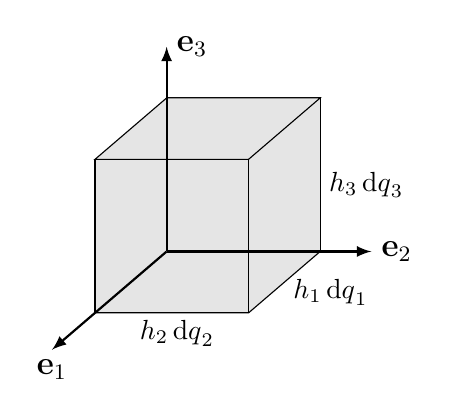
\begin{tikzpicture}[>=latex,scale=1.3]
			\draw[fill = gray!20] (0,0) rectangle (1.5,1.5);
			\draw[fill = gray!20] (-0.7,-0.6) -- (0.8,-0.6) -- (1.5,0) -- (0,0) -- (-0.7,-0.6);
			\draw[fill = gray!20] (-0.7,-0.6) -- (0.8,-0.6) -- (0.8,0.9) -- (-0.7,0.9) -- (-0.7,-0.6);
			\draw[fill = gray!20] (0,1.5) -- (-0.7,0.9) -- (0.8,0.9) -- (1.5,1.5) -- (0,1.5);
			\draw[thick,->] (0,0) -- (-1.12,-0.96)node[below]{\large \(\vb{e}_1\)};
			\draw[thick,->] (0,0) -- (2,0)node[right]{\large \(\vb{e}_2\)};
			\draw[thick,->] (0,0) -- (0,2)node[right]{\large \(\vb{e}_3\)};
			\node at (1.6,-0.4) {\(h_1\dd{q}_1\)};
			\node at (0.1,-0.8) {\(h_2\dd{q}_2\)};
			\node at (1.95,0.65) {\(h_3\dd{q}_3\)};
		\end{tikzpicture}
	\end{figure}

	Here is an easier way to interpret this result based on the alternative definition of divergence from \cref{altdivcurl}. If we take an infinitesimal cuboid \(\mathcal{V}\) of volume \(V\) at point \((q_1,q_2,q_3)\) with sides parallel to the basis vectors \(\vb{e}_1\), \(\vb{e}_2\) and \(\vb{e}_3\).
	\[\div\vb{F}=\lim_{V\to 0}\frac{1}{V}\oiint_\mathcal{S}\vb{F}\vdot\dd{S}\,.\]
	The volume of the cuboid is \(V=h_1h_2h_3\delta q_1\delta q_2\delta q_3\). The area of the surfaces along directions \(\vb{e}_i\) and \(\vb{e}_j\) are given by \(h_ih_j\delta q_i\delta q_j\). Therefore,
	\begin{align*}
		\oiint_\mathcal{S}\vb{F}\vdot\dd{\vb{S}}&\approx[h_1h_2F_3(q_1,q_2,q_3+\delta q_3)-h_1h_2F_3(q_1,q_2,q_3)]\delta q_1\delta q_2+\text{cyclic permutations}\\
		&\approx\pdv{q_3}(h_1h_2F_3)\delta q_1\delta q_2\delta q_3 +\text{cyclic permutations}\,.
	\end{align*}
	Dividing through the volume and taking the limit \(V\to 0\) gives the formula of divergence as claimed.
	\begin{thm}
		The curl of a vector field \(\vb{F}\) in an orthogonal curvilinear coordinate system is given by
		\[\curl\vb{F}=\frac{1}{h_1h_2h_3}\begin{vmatrix}
			h_1\vb{e}_1 & h_2\vb{e}_2 & h_3\vb{e}_3 \\
			\pdv{q_1} & \pdv{q_2} & \pdv{q_3} \\
			h_1F_1 & h_2F_2 & h_3F_3
		\end{vmatrix}\,.\]
	\end{thm}
	\begin{itemize}
		\item Spherical polar coordinates:
		\[\curl\vb{F}=\frac{1}{r^2\sin\theta}\begin{vmatrix}
			\vb{e}_r & r\vb{e}_\theta & r\sin\theta\vb{e}_\phi \\
			\pdv{r} & \pdv{\theta} & \pdv{\phi} \\
			F_r & rF_\theta & r\sin\theta F_\phi
		\end{vmatrix}\]
		\item Cylindrical polar coordinates:
		\[\curl\vb{F}=\frac{1}{\rho}\begin{vmatrix}
			\vb{e}_\rho & \rho\vb{e}_\phi & \vb{e}_z \\
			\pdv{\rho} & \pdv{\phi} & \pdv{z} \\
			F_\rho & \rho F_\phi & F_z
		\end{vmatrix}\]
	\end{itemize}
	\begin{proof}
		\begin{align*}
			\curl{\vb{F}}=\,&\curl\qty(\sum_{i}F_i\vb{e}_i)=\sum_i\curl((h_iF_i)\qty(\frac{\vb{e}_i}{h_i}))\\
			=\,&\sum_{i}\grad(h_iF_i)\cross\frac{\vb{e}_i}{h_i}+\sum_{i}h_iF_i(\curl\grad q_i)\\
			=\,&\sum_{i}\sum_{j}\qty(\frac{1}{h_ih_j}\pdv{(h_iF_i)}{q_j})\vb{e}_j\cross\vb{e}_i\\
			=\,&\frac{\vb{e}_1}{h_2h_3}\qty(\pdv{(h_3F_3)}{q_2}-\pdv{(h_2F_2)}{q_3})+\frac{\vb{e}_2}{h_3h_1}\qty(\pdv{(h_1F_1)}{q_3}-\pdv{(h_3F_3)}{q_1})\\
			&+\frac{\vb{e}_3}{h_1h_2}\qty(\pdv{(h_2F_2)}{q_1}-\pdv{(h_1F_1)}{q_2})\,. & \qed
		\end{align*}
	\end{proof}

	\begin{figure}[ht!]
		\centering
		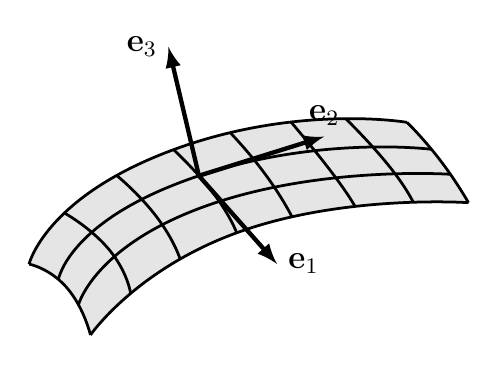
\begin{tikzpicture}[scale=0.6,>=latex]
			\coordinate (A1) at (0,0);
			\coordinate (A2) at (3,2.4);
			\coordinate (A3) at (8,3);
			\coordinate (B1) at (8.7,2.2);
			\coordinate (B2) at (9.3,1.3);
			\coordinate (B3) at (4.5,0.7);
			\coordinate (C1) at (1.3,-1.5);
			\coordinate (C2) at (0.8,-0.5);

			\coordinate (D1) at (0.62,-0.33);
			\coordinate (D2) at (3.45,1.82);
			\coordinate (D3) at (8.51,2.43);

			\coordinate (E1) at (1.05,-0.85);
			\coordinate (E2) at (3.8,1.25);
			\coordinate (E3) at (8.93,1.9);

			\coordinate (F1) at (0.75,1.08);
			\coordinate (F2) at (1.7,0.3);
			\coordinate (F3) at (2.15,-0.62);

			\coordinate (G1) at (1.85,1.88);
			\coordinate (G2) at (2.7,1);
			\coordinate (G3) at (3.2,0.1);

			\coordinate (H1) at (3.05,2.43);
			\coordinate (H2) at (3.9,1.5);
			\coordinate (H3) at (4.4,0.65);

			\coordinate (I1) at (4.25,2.79);
			\coordinate (I2) at (5,1.9);
			\coordinate (I3) at (5.56,1.01);

			\coordinate (J1) at (5.55,3);
			\coordinate (J2) at (6.4,1.95);
			\coordinate (J3) at (6.9,1.22);

			\coordinate (K1) at (6.7,3.08);
			\coordinate (K2) at (7.6,2.1);
			\coordinate (K3) at (8.13,1.31);

			\coordinate (L) at (3.595,1.87);
	
			\draw[white,fill = gray!20, thin] (A1) to [bend left=12] (F1) to [bend left=10] (G1) to [bend left=2] (A2)--(H1)--(I1) to [bend left=2] (J1) to [bend left=5] (K1) to [bend left=5] (A3) to [bend left=5] (D3)--(B1)--(E3)--(B2)--(K3)--(J3)--(I3)--(B3)--(H3)--(G3)--(F3)--(C1)--(E1)--(C2)--(D1) to [bend right=10] (A1);
			\draw[line width=0.35mm] plot [smooth, tension=1.2] coordinates { (A1) (A2) (A3)};
			\draw[line width=0.35mm] plot [smooth, tension=1] coordinates { (B2) (B1) (A3)};
			\draw[line width=0.35mm] plot [smooth, tension=1] coordinates { (C1) (B3) (B2)};
			\draw[line width=0.35mm] plot [smooth, tension=1] coordinates { (A1) (C2) (C1)};
			\draw[line width=0.35mm] plot [smooth, tension=1.2] coordinates { (D1) (D2) (D3)};
			\draw[line width=0.35mm] plot [smooth, tension=1.1] coordinates { (E1) (E2) (E3)};
			\draw[line width=0.35mm] plot [smooth, tension=1] coordinates { (F1) (F2) (F3)};
			\draw[line width=0.35mm] plot [smooth, tension=1] coordinates { (G1) (G2) (G3)};
			\draw[line width=0.35mm] plot [smooth, tension=1] coordinates { (H1) (H2) (H3)};
			\draw[line width=0.35mm] plot [smooth, tension=1] coordinates { (I1) (I2) (I3)};
			\draw[line width=0.35mm] plot [smooth, tension=1] coordinates { (J1) (J2) (J3)};
			\draw[line width=0.35mm] plot [smooth, tension=1] coordinates { (K1) (K2) (K3)};
			\draw[line width=0.55mm,->] (L) -- (5.25,0) node[right]{\large\(\vb{e}_1\)};
			\draw[line width=0.55mm,->] (L) -- (6.25,2.7) node[above]{\large\(\vb{e}_2\)};
			\draw[line width=0.55mm,->] (L) -- (2.95,4.6) node[left]{\large\(\vb{e}_3\)};
		\end{tikzpicture}
	\end{figure}

	Again, there is a more intuitive way to interpret this result based on \cref{altdivcurl}. Take a surface \(\mathcal{S}\) with normal \(\vu{n}=\vb{e}_i\) and area \(A\) at point \((q_1,q_2,q_3)\), bounded by a rectangle with sides along \(\vb{e}_j\) and \(\vb{e}_k\). The component of \(\curl\vb{F}\) along \(\vb{e}_i\) is given by
	\[\vb{e}_i\vdot(\curl\vb{F})=\lim_{A\to 0}\frac{1}{A}\oint_\mathcal{C}\vb{F}\vdot\dd{\vb{x}}\,.\]
	The line integral can be approximated by
	\begin{align*}
		\oint_\mathcal{C}\vb{F}\vdot\dd{\vb{x}}&\approx F_j(q_j,q_k)h_j\delta q_j+F_k(q_j+\delta q_j,q_k)h_k\delta q_k-F_j(q_j,q_k+\delta q_k)h_j\delta q_j-F_k(q_j,q_k)h_k\delta q_k\\
		&\approx \qty[\pdv{q_j}\qty(h_kF_k)-\pdv{q_k}\qty(h_jF_j)]\delta q_j\delta q_k\,.
	\end{align*}
	Dividing by the area \(A=h_j h_k\delta q_j\delta q_k\) and taking the limit \(A\to 0\) gives
	\[\vb{e}_i\vdot(\curl\vb{F})=\frac{1}{h_j h_k}\qty[\pdv{q_j}\qty(h_kF_k)-\pdv{q_k}\qty(h_jF_j)]\,,\]
	which is the components of \(\curl\vb{F}\) as claimed.
	
	\subsubsection{Laplacian in Orthogonal Curvilinear Coordinates}
	\begin{thm}
		The Laplacian operator in an orthogonal curvilinear coordinate system is given by
		\[\laplacian=\frac{1}{h_1h_2h_3}\qty(\pdv{q_1}\qty(\frac{h_2h_3}{h_1}\pdv{q_1})+\pdv{q_2}\qty(\frac{h_3h_1}{h_2}\pdv{q_2})+\pdv{q_3}\qty(\frac{h_1h_2}{h_3}\pdv{q_3}))\,.\]
	\end{thm}
	\begin{itemize}
		\item Spherical polar coordinates:
		\begin{align*}
			\laplacian{\psi}&=\frac{1}{r^2}\pdv{r}(r^2\pdv{\psi}{r})+\frac{1}{r^2\sin\theta}\pdv{\theta}\qty(\sin\theta\pdv{\psi}{\theta})+\frac{1}{r^2\sin^2\theta}\pdv[2]{\psi}{\phi}\\
			&=\frac{1}{r}\pdv[2]{r}(r\psi)+\frac{1}{r^2\sin\theta}\pdv{\theta}\qty(\sin\theta\pdv{\psi}{\theta})+\frac{1}{r^2\sin^2\theta}\pdv[2]{\psi}{\phi}
		\end{align*}
		\item Cylindrical polar coordinates:
		\[\laplacian{\psi}=\frac{1}{\rho}\pdv{\rho} \qty(\rho\pdv{\psi}{\rho})+\frac{1}{\rho^2}\pdv[2]{\psi}{\phi}+\pdv[2]{\psi}{z}\]
	\end{itemize}
	\begin{proof}
		We already have the divergence and gradient, so it is easy to work out.
		\begin{align*}
			\laplacian\psi&=\div\grad{\psi}\\
			&=\frac{1}{h_1h_2h_3}\qty(\pdv{q_1}\qty(\frac{h_2h_3}{h_1}\pdv{\psi}{q_1})+\pdv{q_2}\qty(\frac{h_3h_1}{h_2}\pdv{\psi}{q_2})+\pdv{q_3}\qty(\frac{h_1h_2}{h_3}\pdv{\psi}{q_3}))\,.
		\end{align*}\qed
	\end{proof}
	\newpage

	\section{Green's Functions}
	\subsection{The Dirac Delta Function}
	In the first part of this chapter, we will first try to define a mysterious object called the \textit{Dirac delta function} which, technically, shouldn't even be called a `function'.
	\subsubsection{Definition as Limit of Sequences}
	Consider the function \(\delta_\epsilon(x)\) defined for \(\epsilon>0\) by
	\[\delta_\epsilon(x)\coloneqq\begin{cases}
		0 & x<-\epsilon\\
		\frac{1}{2\epsilon} & -\epsilon\le x\le \epsilon\\
		0 & x>\epsilon\,,
	\end{cases}\]
	then \(\forall\epsilon>0\),
	\[\int_{-\infty}^{\infty}\delta_\epsilon(x)\dd{x}=1\,.\]
	
	For any integrable function \(f(x)\) and constant \(\xi\),
	\[\int_{-\infty}^{\infty}\delta_\epsilon(x-\xi)f(x)\dd{x}=\frac{1}{2\epsilon}\qty(F(\xi+\epsilon)-F(\xi-\epsilon))\,,\]
	where \(F\) is the antiderivative of \(f\). Then in the limit of \(\epsilon\to 0^+\), we can recover
	\begin{align*}
		\lim_{\epsilon\to 0^+}\int_{-\infty}^{\infty}\delta_\epsilon(x-\xi)f(x)\dd{x}&=\lim_{\epsilon\to 0^+}\frac{1}{2\epsilon}\Big(\,\,\quad F(\xi)+\epsilon f(\xi)+\frac{1}{2}\epsilon^2 f'(\xi)+\dots\;&\\
		&\qquad\quad\qquad\,\,\,-F(\xi)+\epsilon f(\xi)-\frac{1}{2}\epsilon^2f'(\xi)+\dots\quad\Big)\\
		&=f(\xi)\,.
	\end{align*}
	
	This inspires us to make the following definition:
	\begin{defn}
		We can view the \textit{Dirac delta function}, \(\delta(x)\), as the limit as \(\epsilon\to 0\) of \(\delta_\epsilon(x)\):
		\[\delta(x)\coloneqq\lim_{\epsilon\to 0^+}\delta_{\epsilon}(x)\,.\]
	\end{defn}
	What are we doing here? When \(\epsilon\) gets smaller, the function \(\delta_\epsilon\) has a higher and higher peak over a narrower and narrower range around \(x=0\). Although it is absolutely clear that neither putting \(\epsilon=0\) directly in the above sequence makes any sense, nor does the \(\epsilon\to 0\) limit really converges to some well-defined function, what we are trying to do here is to create some object that has an infinitely high peak over an infinitely narrow range, and somehow carries a unit weight.
	
	Of course, we can use another sequence of functions to make the same effect. For example, if we alternatively define \(\delta_\epsilon(x)\) as
	\[\delta_\epsilon(x)\coloneqq\frac{\epsilon}{\pi(x^2+\epsilon^2)}\,,\]
	which gives
	\[\int_{-\infty}^{\infty}\delta_\epsilon(x)\dd{x}=1\,.\]
	Now \(\delta_\epsilon\) also has a peak of unit area centred at \(x=0\), which gets sharper as \(\epsilon\to 0_+\). We can identify the Dirac delta function as the \(\epsilon\to 0_+\) limit of this function as well, which also gives
	\begin{align*}
		\int_{-\infty}^{\infty}\delta(x-\xi)f(x)\dd{x}&=\lim_{\epsilon\to 0^+}\int_{-\infty}^{\infty}\delta_\epsilon(x-\xi)f(x)\dd{x}\\
		&=f(\xi)\,.
	\end{align*}
	This sequence of functions even has the nice property that for any \(\epsilon>0\), \(\delta_\epsilon\) is smooth.
	
	This definition of the delta function gives us an expression which turns out to be extremely useful later.
	\begin{prop}\label[prop]{Fourier_one}
		\[\delta(x)=\frac{1}{2\pi}\int_{-\infty}^{\infty}e^{ikx}\dd{k}\,.\]
	\end{prop}
	\begin{proof}
		We note that
		\begin{align*}
			\frac{1}{2\pi}\int_{-\infty}^{\infty}e^{ikx-\epsilon\abs{k}}\dd{k}&=\frac{1}{2\pi}\qty(\int_{-\infty}^{0}e^{ikx+\epsilon k}\dd{k}+\int_{0}^{\infty}e^{ikx-\epsilon k}\dd{k})\\
			&=\frac{\epsilon}{\pi(x^2+\epsilon^2)}\,.
		\end{align*}
		Take \(\epsilon\to 0^+\).\qed
	\end{proof}
	Of course we are doing something weird here. Putting \(x=0\), we get
	\[\delta(0)\stackrel{?}{=}\frac{1}{2\pi}\int_{-\infty}^{\infty}1\dd{x}\,,\]
	which is a complete nonsense. 
	
	\subsubsection{Properties}
	We may identify that the Dirac delta function has an infinitely sharp peak of zero width and has a unit area.
	\[\delta(x)=\begin{cases}
		\infty & x=0\\
		0 & x\ne 0
	\end{cases}\,,\]
	\[\int_{a}^{b}\delta(x)\dd{x}=1 \quad \forall a<0, b>0\,.\]
	This is obviously not what we would normally call a function, but we can get a sense of what it is doing. It provides a surgical strike on the integrand to pick out its value at one particular point:
	\[\int_{-\infty}^{\infty}\delta(x-\xi)f(x)\dd{x}=f(\xi)\,.\]
	This is the continuum analogue of the Kronecker delta.
	
	Despite its absurdity, we can still derive some of its properties.
	\begin{prop}
		\(\delta(x)\) is symmetric.
	\end{prop}
	\begin{proof}
		By the substitution \(k=-l\),
		\[\delta(-x)=\frac{1}{2\pi}\int_{-\infty}^{\infty}e^{-ikx}\dd{k}=-\frac{1}{2\pi}\int_{\infty}^{-\infty}e^{ilx}\dd{l}=\frac{1}{2\pi}\int_{-\infty}^{\infty}e^{ilx}\dd{l}=\delta(x)\,.\]\qed
	\end{proof}
	\begin{prop}
		\(\delta(x)\) is real.
	\end{prop}
	\begin{proof}
		\[\delta^*(x)=\frac{1}{2\pi}\int_{-\infty}^{\infty}e^{-ikx}\dd{k}=\delta(-x)=\delta(x)\,.\]\qed
	\end{proof}

	\subsubsection{Alternative Definition of the Dirac Delta Function}
	We have done a lot of whimsical things above that would certainly drive a mathematician crazy. The major issue of what we have done above is that we have encountered a lot of infinities --- but there is one nice property of Dirac delta that stands out as it involves no infinity. This might help us to define the Dirac delta a bit more sensibly.
	\begin{defn}
		In an alternative (and better) view, \(\delta(x)\) is defined as the \textit{generalised function} (\textit{distribution}) such that for all smooth functions \(f(x)\),
		\[\int_{-\infty}^{\infty}\delta(x-\xi)f(x)\dd{x}=f(\xi)\,.\]
	\end{defn}
	\begin{rem}
		The upshot is that, in this way, \(\delta(x)\) is defined within an integrand as a linear operator, and therefore should always be employed in an integrand. We should never consider taking it out of the integral.
	\end{rem}

	\subsubsection{Derivative of the Delta Function}
	We can be more brave and try to differentiate the Dirac delta. But to do this more legally, we will put it in an integral and see how it does to a well-behaved function. Using integration by parts, we see that
	\[\int_{-\infty}^{\infty}\delta'(x-\xi)f(x)\dd{x}=\qty[\delta(x-\xi)f(x)]^{\infty}_{-\infty}-\int_{-\infty}^{\infty}\delta(x-\xi)f'(x)\dd{x}=-f'(\xi)\,.\]
	\begin{defn}
		The derivative of \(\delta(x)\) is defined as the generalised function such that for all differentiable functions \(f(x)\),
		\[\int_{-\infty}^{\infty}\delta'(x-\xi)f(x)\dd{x}=-f'(\xi)\,.\]
	\end{defn}
	
	Alternatively, the derivative of the delta function may again be defined as the limit of the derivatives of some sequence of functions, \(\delta_\epsilon'\), similar to what we have done at the beginning of this section.
	\subsection{The Heaviside Step Function}
	\begin{defn}
		The \textit{Heaviside step function}, \(H(x)\) is defined for \(x\ne 0\) as
		\[H(x)\coloneqq\begin{cases}
			0 & x<0\\
			1 & x>0\,.
		\end{cases}\]
	\end{defn}
	There are various conventions for the value of the Heaviside step function at \(x=0\). It is not uncommon to choose \(H(0)=\frac{1}{2}\). This is unimportant.
	
	\subsubsection{Properties}
	It is clear to see that this function is discontinuous at \(x=0\):
	\[\lim_{x\to 0^-}H(x)=0\ne1=\lim_{x\to 0^+}H(x)\,.\]
	Therefore, it seems that \(H(x)\) is not differentiable at \(x=0\) --- at least in a normal sense. However, we have just seen that \(\delta(x)\) has a unit area within an infinitely narrow area near \(x=0\). This allows us to make the following identification.
	\begin{prop}
		\[H(x)=\int_{-\infty}^{x}\delta(\xi)\dd{\xi}\,,\]
		and so we may identify
		\[\dv{x} H(x)=\delta(x)\,.\]
	\end{prop}

	\begin{proof}
		\begin{align*}
			\int_{-\infty}^{\infty}H'(x-\xi)f(x)\dd{x}&=\qty[H(x-\xi)f(x)]^{\infty}_{-\infty}-\int_{-\infty}^{\infty}H(x-\xi)f'(x)\dd{x}\\
			&=f(\infty)-\int_{\xi}^{\infty}f'(x)\dd{x}\\
			&=f(\xi)\,.
		\end{align*}\qed
	\end{proof}

	\subsection{Formal Theory of Distributions (Non-examinable)}
	After invented by physicist Dirac, the Dirac delta function quickly becomes ubiquitous in almost all fields in physics, especially in quantum mechanics and quantum field theory. Although we played around with infinities in very dangerous ways when defining this object, it just worked surprisingly well.

	But mathematicians at that time were not satisfied with that. They were trying to find a rigorous mathematical theory to deal with objects like Dirac delta, and it was only achieved until mid-\(20^{\text{th}}\) century when they invented the theory of distributions.

	Of course we are not introducing distribution theory in this course --- this is a very deep subject. Here, we will have a very brief look at some basic principles of it to get a sense of what a distribution really is.
	\subsubsection{Distributions}
	To define a distribution, we must first choose a class of \textit{test functions}, which is the functions that our distribution will act on. For \(\Omega\subseteq\mathbb{R}^n\), the simplest class of test functions are infinitely smooth functions \(\phi\in C^\infty(\Omega)\) that have \textit{compact support}, meaning that there exists a compact set \(K\subset\Omega\) such that \(\phi(\vb{x})=0\) whenever \(x\notin K\). For our purposes, it is fine to just think of such functions to be the ones that take non-zero values only for a finite region in space. Let us denote the space of all test functions \(\mathcal{D}(\Omega)\).
	\begin{defn}
		For a space of test functions \(\mathcal{D}(\Omega)\), a \textit{distribution} \(T\) is defined to be a linear map \(T:\mathcal{D}(\Omega)\to\mathbb{R}\), given by
		\[T:\phi\mapsto T[\phi]\,.\]
	\end{defn}
	\begin{rem}
		\(T\) is not a function on \(\Omega\) itself but rather is a function on the infinite-dimensional space of test functions on \(\Omega\).
	\end{rem}

	The space of distributions with test functions in \(\mathcal{D}(\Omega)\) is denoted \(\mathcal{D}'(\Omega)\). It is an infinite-dimensional vector space because we can add two distributions \(T_1\) and \(T_2\) together, defining the distribution \((T_1+T_2)\) by
	\[(T_1+T_2)[\phi]\coloneqq T_1[\phi]+T_2[\phi]\]
	for all \(\phi\in\mathcal{D}(\Omega)\). We can multiply a distribution by a constant, defining the distribution \((cT)\) by
	\[(cT_1)[\phi]\coloneqq cT_1[\phi]\]
	for all \(\phi\in\mathcal{D}(\Omega)\) and \(c\in\mathbb{R}\). We can also multiply distributions by smooth functions. If \(\psi\in C^\infty(\Omega)\) and \(T\in\mathcal{D}'(\Omega)\) then define the distribution \((\psi T)\) by
	\[(\psi T)[\phi]\coloneqq T[\psi\phi]\,.\]
	\begin{rem}
		In general, there is no way to multiply two distributions together.
	\end{rem}
	The simplest type of distribution is just an ordinary function \(f:\Omega\to\mathbb{R}\) that is locally integrable, meaning that its integral over any compact set converges. To treat \(f\) as a distribution we must say how it acts on any test function \(\phi\in\mathcal{D}(\Omega)\). For example, we can define
	\[f[\phi]\coloneqq(f,\phi)=\int_\Omega f(x)\phi(x)\dd{V}\,,\]
	which is the inner product of \(f\) with \(\phi\). This integral is guaranteed to be well-defined even when \(\Omega\) is non-compact (say, the whole of \(\mathbb{R}^n\)) since \(\phi\) has compact support and \(f\) is locally integrable. By definition, it is easy to check that \(f[\phi]\) is a linear map from \(\mathcal{D}(\Omega)\) to \(R\). In the case where the generalised function is just an ordinary function, the map \(T_f:D(\Omega)\to\mathbb{R}\) just corresponds to the usual inner product between functions.

	The most important example of a generalised function that is not a function is the Dirac delta.
	\begin{defn}
		The \textit{Dirac delta} \(\delta\) is a distribution defined by
		\[\delta[\phi]\coloneqq\phi(\vb{0})\]
		for all \(\phi\in\mathcal{D}(\Omega)\), where \(\vb{0}\) is the origin in \(\mathbb{R}^n\).
	\end{defn}
	\begin{prop}
		\(\delta:\mathcal{D}(\Omega)\to\mathbb{R}\) is a linear map.
	\end{prop}
	\begin{proof}
		\[\delta[c_1\phi_1+c_2\phi_2]=c_1\phi_1(\vb{0})+c_2\phi_2(\vb{0})\,.\]
		The addition on the left is in the vector space of test functions, while the addition on the right is addition in \(\mathbb{R}\).\qed
	\end{proof}
	By analogy with the case where the generalised function is itself a function, it is often convenient to abuse notation and write
	\[T[\phi]=(T,\phi)=\int_\Omega T(\vb{x})\phi(\vb{x})\dd{V}\]
	even for general distributions that are not functions. However, for a general distribution the object \(T(\vb{x})\) is not a function. There is no sense in which \(T:\Omega\to\mathbb{R}\). For example, it is common to write
	\[\delta[\phi]=\int_\Omega\delta(\vb{x})\phi(\vb{x})\dd{V}\]
	for some object \(\delta(\vb{x})\). However, \(\delta(\vb{x})\) cannot possibly be a genuine function. For the integral to be equal to \(\phi(\vb{0})\), the value of \(\delta(\vb{x})\) must vanish whenever \(x\ne 0\). On the other hand, if \(\delta(\vb{0})\) does indeed vanish everywhere except at one point, the integral cannot give the finite answer \(\phi(\vb{0})\) if \(\delta(\vb{x})\) takes any finite value at \(\vb{x}=\vb{0}\). So it is not a genuine function in the sense of being a map from \(\Omega\to\mathbb{R}\). One reason this abusive notation is convenient is that distributions can arise as the limit of a sequence of integrals of usual functions, just as what we have seen before.
	\subsubsection{Differentiation of Distributions}
	In the case that the distribution is just an ordinary function \(f\), we have
	\begin{align*}
		T_{f'}[\phi]&=\int_\Omega f'(x)\phi(x)\dd{x}\\
		&=[f(x)\phi(x)]_\Omega-\int_\Omega f(x)\phi'(x)\dd{x}\\
		&=-T_f[\phi']\,,
	\end{align*}
	where the boundary term vanishes since \(\phi\) has compact support inside \(\Omega\). Let us now define the derivative of a distribution.
	\begin{defn}
		The derivative of a generalised function \(T\) is defined as
		\[T'[\phi]\coloneqq -T[\phi']\]
		for all \(\phi\in\mathcal{D}(\Omega)\).
	\end{defn}
	\begin{rem}
		The idea here is that if we think of our distribution as coming from the limit of a sequence of integrals involving only ordinary functions, this relation will hold for every member of the sequence, and so it will hold for the limiting value of the integrals.
	\end{rem}
	\begin{ex}
		For the delta distribution, we have
		\[\delta'[\phi]=-\delta[\phi']=-\phi'(0)\,.\]
	\end{ex}
	\begin{prop}
		The derivative of the Heaviside step function is the Dirac delta function.
	\end{prop}
	\begin{proof}
		\(H(x)\) defines a generalised function on \(\mathbb{R}\) by
		\[H[\phi]=\int_{-\infty}^{\infty}H(x)\phi(x)\dd{x}=\int_{0}^{\infty}\phi(x)\dd{x}\,,\]
		which converges since \(\phi\) has compact support. \(H(x)\) is not differentiable, or even continuous as a function, but it is perfectly differentiable as a distribution. We have
		\begin{align*}
			H'[\phi]&=-H[\phi']=-\int_{-\infty}^{\infty}H(x)\pdv{\phi}{x}\dd{x}\\
			&=-\int_{0}^{x}\pdv{\phi}{x}\dd{x}\\
			&=\phi(0)-\phi(\infty)=\phi(0)\,,
		\end{align*}
		since \(\phi\) has compact support. Since \(H'[\phi]=\phi(0)=\delta[\phi]\) holds for any test function \(\phi\), we can identify \(H'\) as the distribution \(\delta\).\qed
	\end{proof}
	
	\subsection{Second-order Linear Ordinary Differential Equations}
	One of the most important applications of the Dirac delta is in solving the differential equations. 

	A general second-order linear ODE for \(y(x)\) can be written as
	\[y''+p(x)y'+q(x)y=f(x)\quad \text{or}\quad Ly(x)=f(x)\,,\]
	where \(L\) is the differential operator
	\[L\equiv\dv[2]{x}+p(x)\dv{x}+q(x)\,.\]
	If \(f(x)=0\), then the equation is \textit{homogeneous}, otherwise it is \textit{inhomogeneous}.

	\subsubsection{Homogeneous Second-order ODEs}

	\begin{thm}[The principle of superposition]
		If \(y_1\) and \(y_2\) are solutions to a homogeneous linear differential equation
		\[Ly=0\,,\]
		where \(L\) is a linear differential operator, then they can be superposed to give a third. For any \(\alpha,\beta\in\mathbb{R}\),
		\[y=\alpha y_1+\beta y_2\]
		is also a solution.
	\end{thm}
	
	\begin{cor}
		Suppose \(y_1\) and \(y_2\) are two linearly independent solutions, which means that
		\[\alpha y_1(x)+\beta y_2(x)\equiv 0\implies\alpha=\beta=0\,.\]
		Since the equation is second-order, the general solution will be of the form
		\[y=\alpha y_1+\beta y_2\,.\]
		\(y_1\) and \(y_2\) are commonly referred to as \textit{complementary functions}.
	\end{cor}
	\subsubsection{Inhomogeneous Second-order ODEs}
	\begin{cor}
		If \(y_0(x)\) is any solution of the real inhomogeneous equation
		\[Ly\equiv y''+p(x)y'+q(x)y=f(x)\,,\]
		then the general solution has the form
		\[y(x)=y_0(x)+\alpha y_1(x)+\beta y_2(x)\,,\]
		where \(y_1\) and \(y_2\) are any linearly independent solutions of \(Ly=0\). \(y_0\) is referred to as a \textit{particular solution}.
	\end{cor}
	\subsubsection{The Wronskian}
	If \(y_1\) and \(y_2\) are linearly dependent, then so are \(y_1'\) and \(y_2'\). Hence \(y_1\) and \(y_2\) are linearly dependent only if the equation
	\[\begin{pmatrix}
		y_1 & y_2\\
		y_1' & y_2'
	\end{pmatrix}
	\begin{pmatrix}
		\alpha\\
		\beta
	\end{pmatrix}=\vb{0}\]
	has a non-zero solution for \(\alpha\) and \(\beta\). Conversely, non-zero functions \(y_1\) and \(y_2\) are linearly independent if and only if
	\[\begin{pmatrix}
		y_1 & y_2\\
		y_1' & y_2'
	\end{pmatrix}
	\begin{pmatrix}
		\alpha\\
		\beta
	\end{pmatrix}=\vb{0}\implies\alpha=\beta=0\,.\]
	
	\begin{defn}
		The \textit{Wronskian}, \(W(x)\), of the two solutions is defined to be
		\[W[y_1,y_2]\coloneqq y_1y_2'-y_2y_1'\,.\]
	\end{defn}
	Since \(\mathsf{A}\vb{x}=\vb{0}\) has only the trivial solution iff \(\det(\mathsf{A})\ne 0\), we conclude that \(y_1\) and \(y_2\) are linearly independent iff
	\[\begin{vmatrix}
		y_1 & y_2\\
		y_1' & y_2'
	\end{vmatrix}=y_1y_2'-y_2y_1'=W\ne0\,.\]
	
	\subsubsection{Initial-Value and Boundary-Value Problems}
	Two boundary conditions must be specified to fully determine the solution of a second-order ODE. The general form of a linear boundary condition at a point \(x=a\) is
	\[Ay(a)+By'(a)=E\,,\]
	where \(A, B\) are not both zero. If \(E=0\) the boundary condition is said to be \textit{homogeneous}.

	If two boundary conditions are specified at the same point, then the problem is referred to as an \textit{initial value problem}. If two conditions are specified at different points, then this is a \textit{boundary value problem}.
	
	\subsection{Differential Equations containing Delta Functions}
	Consider the linear second-order ODE
	\[\dv[2]{y}{x}+y=\delta(x)\,.\]
	If \(x\) represent time, then this equation could represent the behaviour of a simple harmonic oscillator in response to an instantaneous force at \(x=0\) with unit impulse.
	
	In regions \(x<0\) and \(x>0\) respectively, the right-hand side vanishes, so the general solution is given by a linear combination of \(\cos x\) and \(\sin x\)
	\[y=\begin{cases}
		\alpha_-\cos x+\beta_-\sin x \quad x<0\\
		\alpha_+\cos x+\beta_+\sin x \quad x>0\,.
	\end{cases}\]
	Since the general solution of a second-order ODE should contain only two arbitrary constants, it should be able to relate \(\alpha_-, \beta_-\) with \(\alpha_+,\beta_+\).
	
	Integrate the differential equation from \(x=-\epsilon\) to \(x=\epsilon\) to obtain
	\[\int_{-\epsilon}^{\epsilon}\pdv[2]{y}{x}\dd{x}+\int_{-\epsilon}^{\epsilon}y(x)\dd{x}=\int_{-\epsilon}^{\epsilon}\delta(x)\dd{x}\,,\]
	\[y'(\epsilon)-y'(-\epsilon)+\int_{-\epsilon}^{\epsilon}y(x)\dd{x}=1\,.\]
	
	Take the limit \(\epsilon\to 0\), assume \(y\) is bounded,
	\[\lim_{\epsilon\to 0}\int_{-\epsilon}^{\epsilon}y(x)\dd{x}=0\,,\]
	\[\implies\qty[\dv{y}{x}]\coloneqq\lim_{\epsilon\to 0}\qty[\dv{y}{x}]^{x=\epsilon}_{x=-\epsilon}=1\,.\]
	Since there is only a finite jump in the derivative of \(y\), \(y\) is continuous. The jump conditions are:
	\[\qty[y]=0,\, \qty[\dv{y}{x}]=1 \text{ at } x=0\,.\]
	
	Applying these conditions, we obtain
	\[\begin{cases}
		\alpha_+-\alpha_-=0\\
		\beta_+-\beta_-=1
	\end{cases}.\]
	Hence the general solution is
	\[y=\begin{cases}
		\alpha\cos x+\beta\sin x & x<0\\
		\alpha\cos x+(\beta+1)\sin x& x>0\,.
	\end{cases}\]
	
	\subsection{Green's Functions}
	\subsubsection{The Green's Function for Two-point Homogeneous Boundary-value Problems}
	Consider an ordinary differential equation
	\[Ly(x)=f(x)\,,\]
	where \(L\) is the general second-order linear differential operator in \(x\):
	\[L=\dv[2]{x}+p(x)\dv{x}+q(x)\]
	with \(p\) and \(q\) being continuous functions, under two homogeneous boundary conditions:
	\[\begin{cases}
		Ay(a)+By'(a)=0\\
		Cy(b)+Dy'(b)=0\,.
	\end{cases}\]

	\begin{defn}
		The \textit{Green's function}, \(G(x;\xi)\), of a differential operator \(L\) for a given set of homogeneous boundary conditions is defined as the response of the system to forcing at a point \(\xi\), such that
		\[\mathcal{L}G(x;\xi)=\delta(x-\xi)\,,\]
		subjected to homogeneous boundary conditions
		\[\begin{cases}
			AG(a;\xi)+BG_x(a;\xi)=0\\
			CG(b;\xi)+DG_x(b;\xi)=0
		\end{cases},\]
		where
		\[\mathcal{L}=\pdv[2]{x}+p(x)\pdv{x}+q(x)\]
		\[G_x(x;\xi)=\pdv{G}{x}(x;\xi)\,.\]
	\end{defn}
	
	\begin{thm}
		The solution to the second-order linear differential equation \(Ly=f\) is
		\[y(x)=\int_{a}^{b}G(x;\xi)f(\xi)\dd{\xi}\,,\]
		where \(G(x;\xi)\) is the Green's function.
	\end{thm}
	\begin{rem}
		We may view Green's function as an inverse differential operator
		\[Ly=f \implies y=L^{-1}f=\int_{a}^{b}\dd{\xi}G(x;\xi)\;f(\xi)\,.\]
	\end{rem}	
	\begin{proof}
		Our proposed solution satisfies both of the boundary conditions
		\[Ay(a)+By'(a)=\int_{a}^{b}(AG(a;\xi)+BG_x(a;\xi))f(\xi)\dd{\xi}=0\]
		\[Cy(b)+Dy'(b)=\int_{a}^{b}(CG(b;\xi)+DG_x(b;\xi))f(\xi)\dd{\xi}=0\]
		and the inhomogeneous equation
		\begin{align*}
			Ly(x)&=\int_{a}^{b}\mathcal{L}G(x;\xi)f(\xi)\dd{\xi}\\
			&=\int_{a}^{b}\delta(x-\xi)f(\xi)\dd{\xi}=f(x)\,.
		\end{align*}\qed
	\end{proof}

	\subsubsection{Properties of the Green's Functions}
	\begin{lem}\label[lem]{propgreen}
		\(G\) is continuous and there is a unit jump in \(\pdv{G}{x}\) at \(x=\xi\).
	\end{lem}
	\begin{proof}
		Integrate both sides of
		\[\mathcal{L}G(x;\xi)=\delta(x-\xi)\]
		from \(\xi-\epsilon\) to \(\xi+\epsilon\) for \(\epsilon>0\) and consider the limit \(\epsilon\to 0\):
		\begin{align*}
			1&=\lim_{\epsilon\to 0}\int_{\xi-\epsilon}^{\xi+\epsilon}\mathcal{L}G\dd{x}\\
			&=\lim_{\epsilon\to 0}\int_{\xi-\epsilon}^{\xi+\epsilon}\qty(\pdv[2]{G}{x}+p\pdv{G}{x}+qG)\dd{x}\\
			&=\lim_{\epsilon\to 0}\int_{\xi-\epsilon}^{\xi+\epsilon}\pdv{x}\qty(\pdv{G}{x}+pG)\dd{x}+\lim_{\epsilon\to 0}\int_{\xi-\epsilon}^{\xi+\epsilon}\qty(-\dv{p}{x}G+qG)\dd{x}\\
			&=\lim_{\epsilon\to 0}\qty[\pdv{G}{x}+pG]_{x=\xi-\epsilon}^{x=\xi+\epsilon}-\lim_{\epsilon\to 0}\int_{\xi-\epsilon}^{\xi+\epsilon}\qty(\dv{p}{x}-q)G\dd{x}\,.
		\end{align*}
		Suppose \(G(x;\xi)\) is bounded near \(x=\xi\), and since \(p\) and \(q\) are continuous, the latter term vanishes to give
		\[\lim_{\epsilon\to 0}\qty[\pdv{G}{x}+pG]_{x=\xi-\epsilon}^{x=\xi+\epsilon}=1\,.\]
		This implies that the jump in the derivative of \(G\) is bounded, so \(G\) must be continuous. We conclude that
		\[\lim_{\epsilon\to 0}\qty[G(x;\xi)]_{x=\xi-\epsilon}^{x=\xi+\epsilon}=0\,,\quad\lim_{\epsilon\to 0}\qty[\pdv{G}{x}]_{x=\xi-\epsilon}^{x=\xi+\epsilon}=1\,.\]\qed
	\end{proof}
 	\subsubsection{Construction of the Green's Function}
	When \(x\ne\xi\), \(G\) satisfies the homogeneous equation, so for both \(x>\xi\) and \(x<\xi\), we can express \(G\) in terms of solutions of the homogeneous equation. Suppose that \(\{y_1,y_2\}\) are a basis of linearly independent solutions to the homogeneous equation \(\mathcal{L}y=0\) on \([a,b]\). We define this basis by requiring
	\[\begin{cases}
		Ay_1(a)+By_1'(a)=0\\
		Cy_2(b)+Dy_2'(b)=0
	\end{cases},\]
	i.e. each of the solutions obeys one of the homogeneous boundary conditions. On \([a,\xi)\), the Green's function obeys \(\mathcal{L}G=0\) and
	\[AG(a;\xi)+B\pdv{G}{x}\qty(a;\xi)=0\,.\]
	Since any homogeneous solution to \(\mathcal{L}y=0\) satisfying \(Ay(a)+By'(a)=0\) must be proportional to \(y_1(x)\), with a proportionality constant independent of \(x\). Thus we can set
	\[G(x;\xi)=\alpha(\xi)y_1(x)\quad \text{for }x\in[a,\xi)\,.\]
	Similarly on \((\xi,b]\) the Green's function must be proportional to \(y_2(x)\) so we get
	\[G(x;\xi)=\beta(\xi)y_2(x)\quad \text{for }x\in(\xi,b]\,.\]

	Now we can determine how these constructions defined at \(x\in[a,b]\setminus\{\xi\}\) can be joined together at \(x=\xi\). From \cref{propgreen}, we must have
	\[\begin{cases}
		\beta(\xi)y_2(\xi)-\alpha(\xi)y_1(\xi)=0\\
		\beta(\xi)y'_2(\xi)-\alpha(\xi)y'_1(\xi)=1\,.
	\end{cases}\]
	Rearranging gives
	\[\begin{pmatrix}
		y_1 & y_2\\
		y_1' & y_2'
	\end{pmatrix}\begin{pmatrix}
		-\alpha\\
		\beta
	\end{pmatrix}=\begin{pmatrix}
		0\\
		1
	\end{pmatrix}\,.\]
	So a solution exists if
	\[W\equiv\begin{vmatrix}
		y_1 & y_2\\
		y_1' & y_2'
	\end{vmatrix}\ne 0\,,\]
	which gives
	\[\alpha(\xi)=\frac{y_2(\xi)}{W(\xi)}\quad \text{and} \quad \beta(\xi)=\frac{y_1(\xi)}{W(\xi)}\,.\]

	\begin{thm}\label{bcgreens}
		For a linear second-order differential operator \(L\) subjected to homogeneous boundary conditions, the Green's function is given by
		\[G(x;\xi)=\left\{\begin{aligned}
			\frac{y_1(x)y_2(\xi)}{W(\xi)} & \quad\text{for }x\in[a,\xi)\\
			\frac{y_1(\xi)y_2(x)}{W(\xi)} & \quad\text{for }x\in[\xi,b]\,,
		\end{aligned}\right.\]
		where \(y_1\) and \(y_2\) satisfy the boundary conditions at \(a\) and \(b\) respectively.
	\end{thm}
	
	\begin{ex}
		Solve
		\[y''(x)+y(x)=f(x),\quad y(0)=y(1)=0\,.\]
		
		The complementary functions satisfying left and right boundary conditions are
		\[y_1=\sin{x},\, y_2=\sin(x-1)\,,\]
		and the Wronskian is
		\[W=y_1y_2'-y_2y_1'=\sin{x}\cos(x-1)-\sin(x-1)\cos{x}=\sin{1}\,.\]
		Thus,
		\[G(x;\xi)=\left\{\begin{aligned}
			\frac{\sin{x}\sin(\xi-1)}{\sin{1}} & \quad 0\le x\le \xi\\
			\frac{\sin{\xi}\sin(x-1)}{\sin{1}} & \quad \xi\le x\le 1\,.
		\end{aligned}\right.\]
		
		The solution is given by
		\begin{align*}
			y(x)&=\int_{0}^{1}G(x;\xi)f(\xi)\dd{\xi}\\
			&=\frac{\sin(x-1)}{\sin{1}}\int_{0}^{x}\sin{\xi} f(\xi)\dd{\xi}+\frac{\sin{x}}{\sin{1}}\int_{x}^{1}\sin(\xi-1)f(\xi)\dd{\xi}\,.
		\end{align*}
	\end{ex}
	
	\subsubsection{The Green's Function for Homogeneous Initial-Value Problems}
	Suppose the boundary conditions are instead
	\[y(a)=y'(a)=0\,.\]
	For \(x\in[a,\xi)\), choose the complementary functions such that \(y_1(a)=0\) and \(y_2'(a)=0\), and the Green's function is given by
	\[G(x;\xi)=\alpha(\xi)y_1(x)+\beta(\xi)y_2(x)\,.\]
	Apply boundary conditions to the Green's function, then we get
	\[\begin{cases}
		\alpha y_1(a)+\beta y_2(a)=0\\
		\alpha y'_1(a)+\beta y'_2(a)=0
	\end{cases}\implies\begin{cases}
		\alpha=0\\
		\beta=0\,.
	\end{cases}\]
	This implies that
	\[G=0\quad\text{for }x\in[a,\xi)\,.\]

	For \(x\in[\xi,\infty)\), we again write the Green's function as
	\[G(x;\xi)=\lambda(\xi)y_1(x)+\mu(\xi)y_2(x)\,.\]
	Apply \cref{propgreen} at \(x=\xi\), we get
	\[\begin{cases}
		\lambda y_1(\xi)+\mu y_2(\xi)=0\\
		\lambda y'_1(\xi)+\mu y'_2(\xi)=1\,,
	\end{cases}\]
	which organises to
	\[\begin{pmatrix}
		y_1(\xi) & y_2(\xi)\\
		y_1'(\xi) & y_2'(\xi)
	\end{pmatrix}\begin{pmatrix}
		\lambda\\
		\mu
	\end{pmatrix}=\begin{pmatrix}
		0\\
		1
	\end{pmatrix}\,,\]
	with solutions
	\[\lambda=-\frac{y_2(\xi)}{W(\xi)}\quad \text{and} \quad \mu=\frac{y_1(\xi)}{W(\xi)}\,.\]
	
	\begin{thm}
		For a linear second-order differential operator \(L\) subjected to homogeneous initial conditions, Green's function is given by
		\[G(x;\xi)=\left\{\begin{aligned}
			& \qquad\qquad\,\,\,\,\;0 && \text{for }a\le x<\xi\\
			&\frac{y_1(\xi)y_2(x)-y_1(x)y_2(\xi)}{W(\xi)} && \text{for }x\ge\xi\,.
		\end{aligned}\right.\]
		where \(y_1\) and \(y_2\) satisfy the boundary conditions \(y(a)=0\) and \(y'(a)=0\) respectively.
	\end{thm}
	
	\subsubsection{Inhomogeneous Boundary Conditions}
	To solve an inhomogeneous equation under inhomogeneous boundary conditions
	\[Ly=f\,,\]
	first solve the homogeneous equation \(Ly=0\) for the inhomogeneous boundary conditions, which gives a solution \(y_{\text{ibc}}\).
	
	Then solve the inhomogeneous equation \(Ly=f\) for the homogeneous boundary conditions (perhaps using Green's functions) to give a solution \(y_{\text{hbc}}\).
	
	By linearity, \(y=y_{\text{ibc}}+y_{\text{hbc}}\) satisfies the inhomogeneous equation with inhomogeneous boundary conditions.

	\newpage

	\section{Fourier Transforms}
	\subsection{Fourier Transforms}
	When we have a periodic function, we express it in terms of a Fourier series. In this chapter, we want to generalise this result to non-periodic functions.
	\begin{defn}
		For a suitably well-behaved function \(f:\mathbb{R}\to\mathbb{C}\), its \textit{Fourier transform} \(\tilde{f}:\mathbb{R}\to\mathbb{C}\) is defined as
		\[\mathcal{F}[f(x)]\equiv\tilde{f}(k)\coloneqq\int_{-\infty}^{\infty}e^{-ikx}f(x)\dd{x}\,.\]
	\end{defn}
	\begin{rem}
		You may encounter a lot of different conventions when defining the Fourier transform. Sometimes there will be a normalising factor \(\frac{1}{\sqrt{2\pi}}\), sometimes the \(-ikx\) will be replaced by \(+ikx\) --- or sometimes even \(\pm 2\pi ikx\). We will stick to the most common convention in the mathematical community defined above.
	\end{rem}
	
	The Fourier transform transforms between complex-valued functions, so the transform of a real function does not necessarily remain real.
	\begin{prop}
		If \(f(x)\) is both real and even, then \(\tilde{f}\) is real.
	\end{prop}
	\begin{proof}
		\begin{align*}
			\tilde{f}^*(k)&=\int_{-\infty}^{\infty}e^{ikx}f^*(x)\dd{x}\\
			&=\int_{-\infty}^{\infty}e^{ikx}f(-x)\dd{x}\\
			&=\int_{-\infty}^{\infty}e^{-iky}f(y)\dd{y}\\
			&=\tilde{f}(k)
		\end{align*}\qed
	\end{proof}
	\begin{prop}
		If \(f(x)\) is both real and odd, then \(\tilde{f}\) is purely imaginary.
	\end{prop}
	\begin{proof}
		Similar to above.\qed
	\end{proof}
	\begin{rem}
		A necessary condition for \(\tilde{f}(k)\) to exist (as a normal function, not as a distribution) for all real values of \(k\) is that \(f(x)\to 0\) as \(x\to\pm\infty\). Otherwise, the Fourier integral does not converge (e.g. for \(k=0\)).
	
		A set of sufficient conditions for \(\tilde{f}(k)\) to exist is that \(f(x)\) have bounded variation, a finite number of discontinuities and be absolutely integrable, i.e.
		\[\int_{-\infty}^{\infty}\abs{f(x)}\dd{x}<\infty\,.\]
	\end{rem}
	
	\subsubsection{Examples of Fourier Transforms}
	\begin{enumerate}[topsep=0pt]
		\item \(e^{-b\abs{x}}\), \(b>0\).
		\begin{align*}
			\mathcal{F}\qty[e^{-b\abs{x}}]&=\int_{-\infty}^{\infty}e^{-ikx-b\abs{x}}\dd{x}\\
			&=\frac{2b}{k^2+b^2}
		\end{align*}
		
		\item \(\cos(ax)e^{-b\abs{x}}\).
		\begin{align*}
			\mathcal{F}\qty[\cos(ax)e^{-b\abs{x}}]&=\frac{1}{2}\int_{-\infty}^{\infty}(e^{iax}+e^{-iax})e^{-ikx-b\abs{x}}\dd{x}\\
			&=b\qty(\frac{1}{(a-k)^2+b^2}+\frac{1}{(a+k)^2+b^2})
		\end{align*}
		
		\item \(\sin(ax)e^{-b\abs{x}}\).
		\begin{align*}
			\mathcal{F}\qty[\sin(ax)e^{-b\abs{x}}]&=\frac{1}{2i}\int_{-\infty}^{\infty}(e^{iax}-e^{-iax})e^{-ikx-b\abs{x}}\dd{x}\\
			&=-ib\qty(\frac{1}{(a-k)^2+b^2}-\frac{1}{(a+k)^2+b^2})
		\end{align*}
		
		\item Gaussian.
		\begin{align*}
			\mathcal{F}\qty[\frac{1}{\sqrt{2\pi}\epsilon}e^{-\frac{x^2}{2\epsilon^2}}]&=\frac{1}{\sqrt{2\pi}\epsilon}\int_{-\infty}^{\infty}\exp(-\frac{x^2}{2\epsilon^2}-ikx)\dd{x}\\
			&=\frac{1}{\sqrt{2\pi}\epsilon}\int_{-\infty}^{\infty}\exp(-\frac{1}{2}\qty(\frac{x}{\epsilon}+i\epsilon k)^2-\frac{1}{2}\epsilon^2k^2)\dd{x}\\
			&=\frac{1}{\sqrt{2\pi}}\exp(-\frac{1}{2}\epsilon^2k^2)\int_{-\infty}^{\infty}\exp(-\frac{1}{2}y^2)\dd{y} &\text{substitution }x=\epsilon y-i\epsilon^2 k\\
			&=\exp(-\frac{1}{2}\epsilon^2k^2)
		\end{align*}
		\begin{rem}
			The Fourier transform of a Gaussian of width \(\epsilon\) is a Gaussian of width \(\epsilon^{-1}\).
		\end{rem}

		\item Dirac delta function.
		\begin{align*}
			\mathcal{F}\qty[\delta(x-a)]&=\int_{-\infty}^{\infty}\delta(x-a)e^{-ikx}\dd{x}\\
			&=e^{-ika}			
		\end{align*}
		Hence the Fourier transform of \(\delta(x)\) is \(1\). Recall that the Dirac delta function can be considered as the limit of a Gaussian as \(\epsilon\to 0^+\).

		\item Constant function.
		\[\mathcal{F}[a]=a\int_{-\infty}^{\infty}e^{-ikx}\dd{x}\,.\]
		This clearly violates our previous claim that in order to have a Fourier transform in the sense of a normal function, we must have \(f(x)\to 0\) as \(x\to\pm\infty\). Therefore, this Fourier transform only exists in the sense of a distribution. Recall the expression of the delta function in \cref{Fourier_one} --- this is exactly what we have here. We can identify
		\[\int_{-\infty}^{\infty}e^{-ikx}=2\pi\delta(k)\,,\]
		so
		\[\mathcal{F}[a]=2\pi a\delta(k)\,.\]
		
		\item Heaviside step function. A direct Fourier transform is problematic:
		\begin{align*}
			\mathcal{F}\qty[H(x-a)]&=\int_{-\infty}^{\infty}H(x-a)e^{-ikx}\dd{x}\\
			&=\int_{a}^{\infty}e^{-ikx}\\
			&=\qty[\frac{e^{-ikx}}{-ik}]_{a}^{\infty}\,,
		\end{align*}
		but the limit \(\lim\limits_{x\to\infty}e^{-ikx}\) does not exist. This is another case that the function is not absolutely integrable, so we need a convergent regularisation of it.
		
		We may first find the Fourier transform of \(H(x-a)e^{-\epsilon(x-a)}\), then take the limit \(\epsilon\to 0^+\). Doing so, we have
		\begin{align*}
			\mathcal{F}[H(x-a)e^{-\epsilon(x-a)}]&=\int_{-\infty}^{\infty}H(x-a)e^{-\epsilon(x-a)-ikx}\dd{x}\\
			&=\qty[\frac{e^{-\epsilon(x-a)-ikx}}{-\epsilon-ik}]_a^\infty\\
			&=\frac{e^{-ika}}{\epsilon+ik}
		\end{align*}
		For any \(k\ne 0\), we are safe to ignore the \(\epsilon\) in the denominator as we take the \(\epsilon\to 0^+\) limit, and therefore we have
		\[\mathcal{F}[H(x-a)]=\lim_{\epsilon\to 0^+}\mathcal{F}[H(x-a)e^{-\epsilon(x-a)}]=\frac{e^{-ika}}{ik}\,.\]
		However, when \(k=0\), we are not allowed to do so. We have to work out the Fourier transform at this point separately. We have
		\[\mathcal{F}[H(x-a)](0)=\int_{a}^{\infty}1\dd{x}=\frac{1}{2}\int_{-\infty}^{\infty}\dd{x}\,.\]
		This integral does not converge, but it is again exactly the expression of delta function we met in \cref{Fourier_one} with \(x=0\), so
		\[\mathcal{F}[H(x-a)](0)=\pi\delta(0)\,.\]
		Combining the above results, we have
		\[\mathcal{F}[H(x-a)]=\frac{e^{-ika}}{ik}+\pi\delta(k)\,,\]
		where we used the property that \(\delta(k)=0\) for \(k\ne 0\).

		If you think the proof above makes no sense, you absolutely are right. This result must be interpreted in the sense of a distribution, and is better proven using something called the Sokhotski--Plemelj identity in distribution theory. We are of course not doing this here.

		\begin{rem}
			\(ik\mathcal{F}[H(x-a)]=\mathcal{F}[\delta(x-a)]\).
		\end{rem}

		\item Top-hat function, \(g(x)\), defined by
		\[g(x)=\begin{cases}
			c & a<x<b\\
			0 & \text{otherwise}\,.
		\end{cases}\]
		\[\tilde{g}(k)=\int_{a}^{b}ce^{-ikx}\dd{x}=\frac{ic}{k}(e^{-ikb}-e^{-ika})\]
		
		For instance, if \(a=-1\), \(b=1\), \(c=1\),
		\[\tilde{g}(k)=\frac{2\sin k}{k}\,.\]
	\end{enumerate}
	
	\subsection{Fourier Inversion Theorem}
	The nice thing about the Fourier transform is that you can transform it back easily.
	\begin{thm}[Fourier inversion theorem]
		The inverse Fourier transform acting on \(\tilde{f}(k)\) that recovers \(f(x)\) is given by
		\[\mathcal{I}[\tilde{f}]\coloneqq\frac{1}{2\pi}\int_{-\infty}^{\infty}e^{ikx}\tilde{f}(k)\dd{k}=f(x)\,.\]
	\end{thm}
	
	\begin{proof}
		\begin{align*}
			\frac{1}{2\pi}\int_{-\infty}^{\infty}e^{ikx}\tilde{f}(k)\dd{k}&=\frac{1}{2\pi}\int_{-\infty}^{\infty}e^{ikx}\qty(\int_{-\infty}^{\infty}e^{-iks}f(s)\dd{s})\dd{k}\\
			&=\int_{-\infty}^{\infty}\qty(\frac{1}{2\pi}\int_{-\infty}^{\infty}e^{ik(x-s)}\dd{k})f(s)\dd{s} & \text{swap integration order}\\
			&=\int_{-\infty}^{\infty}f(s)\delta(x-s)\dd{s}\\
			&=f(x)\,.
		\end{align*}\qed
	\end{proof}
	
	\begin{cor}
		If \(g(k)=\tilde{f}(k)\), then \(\tilde{g}(k)=2\pi f(-k)\).
	\end{cor}
	We can take advantage of this when calculating the Fourier series.
	\begin{ex}
		Find the Fourier transform of \((x^2+b^2)^{-1}\).

		We have worked out
		\[\mathcal{F}\qty[e^{-b\abs{x}}]=\frac{2b}{k^2+b^2}\,.\]
		Applying the observation above, we get
		\[\mathcal{F}\qty[\frac{1}{x^2+b^2}](k)=\frac{\pi}{b}e^{-b\abs{k}}\,.\]
	\end{ex}
	
	\subsection{Properties of Fourier Transforms}
	\begin{prop}\label[prop]{ftdif}
		The Fourier transform has the following properties.
		\begin{enumerate}[topsep=0pt]
			\item \textit{Linearity.} For constants \(\alpha,\beta\in\mathbb{C}\),
			\[\mathcal{F}[\alpha f(x)+\beta g(x)]=\alpha\mathcal{F}[f(x)]+\beta\mathcal{F}[g(x)]\,.\]
			\item \textit{Rescaling.} For real constant \(\alpha\in\mathbb{R}\),
			\[\mathcal{F}[f(\alpha x)]=\frac{1}{\abs{\alpha}}\tilde{f}\qty(\frac{k}{\alpha})\,.\]
			\item \textit{Translation.} For real constant \(\alpha\in\mathbb{R}\),
			\[\mathcal{F}[f(x-\alpha)]=e^{-ik\alpha}\mathcal{F}[f(x)]\]
			\item \textit{Exponential.} For constant \(\alpha\in\mathbb{C}\),
			\[\mathcal{F}[e^{i\alpha x}f(x)](k)=\mathcal{F}[f(x)](k-\alpha)\,.\]
			\item \textit{Duality.} If \(g(x)=\tilde{f}(x)\), then
			\[\tilde{g}(k)=2\pi f(-k)\,.\]
			\item \textit{Complex conjugation and parity inversion.} For \(k\in\mathbb{R}\),
			\[\mathcal{F}[f^*](k)=\mathcal{F}[f](-k)^*\,.\]
			\item \textit{Symmetry.} If \(f(-x)=\pm f(x)\) i.e. \(f\) is even or odd, then
			\[\tilde{f}(-k)=\pm\tilde{f}(k)\,.\]
			\item \textit{Differentiation.}
			\[\mathcal{F}\qty[\dv[n]{f}{x}]=(ik)^n\tilde{f}\,.\]
			\item \textit{Multiplication by \(x\).}
			\[\mathcal{F}[x f(x)]=i\dv{\tilde{f}}{k}\,.\]
		\end{enumerate}
	\end{prop}
	\begin{rem}
		Fourier transforms allow a simple representation of derivatives of \(f(x)\) in Fourier space. This has important consequences for solving differential equations.
	\end{rem}
	\begin{proofskip}
		\begin{enumerate}[parsep=1em]
			\item Trivial by the linearity of multiplication and integration.
			\item Let \(g(x)=f(\alpha x)\),
			\begin{align*}
				\tilde{g}(k)&=\int_{-\infty}^{\infty}e^{-ikx}f(\alpha x)\dd{x}\\
				&=\frac{\text{sgn }\alpha}{\alpha}\int_{-\infty}^{\infty}e^{-i\frac{k}{\alpha}y}f(y)\dd{y}\\
				&=\frac{1}{\abs{\alpha}}\tilde{f}\qty(\frac{k}{\alpha})\,.
			\end{align*}
			\item
			\begin{align*}
				\mathcal{F}[f(x-\alpha)]&=\int_{-\infty}^{\infty}e^{-ikx}f(x-\alpha)\dd{x}\\
				&=\int_{-\infty}^{\infty}e^{-ik(y+\alpha)}f(y)\dd{y}\\
				&=e^{-ik\alpha}\mathcal{F}[f(x)]\,.
			\end{align*}
			\item
			\begin{align*}
				\mathcal{F}[e^{i\alpha x}f(x)](k)&=\int_{-\infty}^{\infty}e^{-i(k-\alpha)x}f(x)\dd{x}\\
				&=\mathcal{F}[f(x)](k-\alpha)\,.
			\end{align*}
			\item
			\begin{align*}
				\tilde{g}(k)&=\int_{-\infty}^{\infty}e^{-ikx}\tilde{f}(x)\dd{x}\\
				&=2\pi f(-k)\,.
			\end{align*}
			\item
			\begin{align*}
				\mathcal{F}[f^*](k)&=\int_{-\infty}^{\infty}e^{-ikx}f^*(x)\dd{x}\\
				&=\qty(\int_{-\infty}^{\infty}e^{ikx}f(x)\dd{x})^*\\
				&=\mathcal{F}[f](-k)^*\,.
			\end{align*}
			\item
			\begin{align*}
				\tilde{f}(-k)&=\int_{-\infty}^{\infty}f(x)e^{ikx}\\
				&=\int_{-\infty}^{\infty}\pm f(-x)e^{ikx}\dd{x}\\
				&=\pm\int_{-\infty}^{\infty}f(y)e^{-iky}\dd{y}\\
				&=\pm\tilde{f}(k)\,.
			\end{align*}
			\item By differentiating the inverse Fourier theorem, we obtain
			\[\dv{x} f(x)=\frac{1}{2\pi}\int_{-\infty}^{\infty}e^{ikx}\qty(ik\tilde{f}(k))\dd{k}=\mathcal{I}\qty[ik\tilde{f}]\,.\]
			Fourier transform this equation, and we obtain
			\[\mathcal{F}\qty[\dv{f}{x}]=\mathcal{F}\qty[\mathcal{I}\qty[ik\tilde{f}]]=ik\tilde{f}\,,\]
			and hence
			\[\mathcal{F}\qty[\dv[n]{f}{x}]=(ik)^n\tilde{f}\,.\]
					
			Alternatively, here is another proof.
			\begin{align*}
				\mathcal{F}\qty[\dv{f}{x}]&=\int_{-\infty}^{\infty}f'(x)e^{-ikx}\dd{x}\\
				&=\qty[f(x)e^{-ikx}]_{-\infty}^{\infty}-\int_{-\infty}^{\infty}-ikf(x)e^{-ikx}\dd{x}\\
				&=ik\tilde{f}(k)\,,
			\end{align*}
			where the former part vanishes because \(f(x)\to 0\) as \(x\to\pm\infty\) for the Fourier transform to converge.		
			\item Differentiate the Fourier transform with respect to \(k\), we obtain
			\[\dv{k} \tilde{f}(k)=\int_{-\infty}^{\infty}e^{-ikx}(-ixf(x))\dd{x}\,.\]
			After multiplying by \(i\), we can deduce that
			\[\mathcal{F}[x f(x)]=i\dv{\tilde{f}}{k}\,.\]
		\end{enumerate}\qed
	\end{proofskip}
	
	\subsection{Fourier Series}
	We claimed that the Fourier transform is the generalisation of Fourier series to non-periodic functions. We will illustrate this connection here.
	\begin{lem}[Fourier series]
		Suppose that \(f:\mathbb{R}\to\mathbb{C}\) is a periodic function with period \(L\), then \(f\) can be represented by a \textit{Fourier series}
		\[f(x)=\sum_{n=-\infty}^{\infty}a_n \exp(\frac{2\pi inx}{L})\,,\]
		where
		\[a_n=\frac{1}{L}\int_{-\frac{1}{2}L}^{\frac{1}{2}L}f(x)\exp(-\frac{2\pi inx}{L})\dd{x}\,.\]
	\end{lem}
	
	As \(L\to\infty\) (\(f(x)\) becomes non-periodic), the increment between successive wavenumbers in its Fourier series, \(\Delta k=\frac{2\pi}{L}\), becomes vanishingly small. Therefore, the spectrum for allowed wavenumbers \(k_n\) becomes a continuum.
	
	Rewrite the formula of the Fourier series as
	\[f(x)=\frac{1}{2\pi}\sum_{n=-\infty}^{\infty}\tilde{f}(k_n)\exp(ixk_n)\Delta k\]
	\[\tilde{f}(k_n)=\int_{-\frac{1}{2}L}^{\frac{1}{2}L}f(x)\exp(-ixk_n)\dd{x}\,,\]
	where
	\[\tilde{f}(k_n)=La_n=\frac{2\pi a_n}{\Delta k}\,.\]
	
	We then see that in the limit \(\Delta k\to0\) and \(L\to\infty\)
	\[f(x)=\frac{1}{2\pi}\int_{-\infty}^{\infty}\tilde{f}(k)\exp(ikx)\dd{k}\]
	\[\tilde{f}(k)=\int_{-\infty}^{\infty}f(x)\exp(-ikx)\dd{x}\,.\]
	
	\subsection{Convolution}
	\subsubsection{Definition of Convolution}
	\begin{defn}
		The \textit{convolution}, \(f*g\), of a function \(f(x)\) with another function \(g(x)\) is defined by
		\[(f*g)(x)\coloneqq\int_{-\infty}^{\infty}f(y)g(x-y)\dd{y}\,.\]
	\end{defn}
	\begin{rem}
		The convolution expresses the amount of overlap of one function \(g\) as it is shifted over another function \(f\).
	\end{rem}
	
	\begin{prop}
		The convolution operator is commutative.
		\[f*g=g*f\]
	\end{prop}
	\begin{proof}
		Let \(z=x-y\).
		\begin{align*}
			f*g(x)&=\int_{-\infty}^{\infty}f(y)g(x-y)\dd{y}\\
			&=-\int_{+\infty}^{-\infty}f(x-z)g(z)\dd{z}\\
			&=\int_{-\infty}^{\infty}g(z)f(x-z)\dd{z}\,.
		\end{align*}\qed
	\end{proof}
	
	\subsubsection{Interpretation}
	\begin{prop}
		If \(x\) and \(y\) are two random variables with probability densities \(f(x)\) and \(g(y)\). Let the distribution of their sum, \(z=x+y\), be \(h(z)\). The probability density function of \(z\) is given by
		\[h=f*g\,.\]
	\end{prop}
	
	\begin{proof}
		For any given value of \(x\), the probability that \(z\) lies in the range
		\[z_0<z<z_0+\delta z\]
		is the probability that \(y\) lies in the range
		\[z_0-x<y<z_0-x+\delta_z\,,\]
		which is \(g(z_0-x)\delta z\). Therefore, the probability that \(z\) lies in the same range for all \(x\) is
		\[h(z_0)\delta z=\int_{-\infty}^{\infty}f(x)g(z_0-x)\delta z\dd{x}\,.\]
		This implies that \(h=f*g\).\qed
	\end{proof}
	
	\begin{rem}
		The effect of measuring, observing or processing scientific data can often be described as a convolution between the data with certain functions. For instance, the gravitational potential of an object
		\[\Phi(\vb{x})=-G\int \frac{\rho(\vb{y})}{\abs{\vb{x}-\vb{y}}}\dd{\vb{y}}\]
		is the convolution of the mass density \(\rho(\vb{x})\) with the potential of a point mass \(-\frac{G}{\abs{\vb{x}}}\).
	\end{rem}
	
	\subsubsection{The Convolution Theorem}
	\begin{thm}[The convolution theorem]\label{conthm}	
		If the functions \(f\) and \(g\) have Fourier transforms \(\mathcal{F}[f]\) and \(\mathcal{F}[g]\) respectively, then
		\[\mathcal{F}[f*g]=\mathcal{F}[f]\mathcal{F}[g]\,.\]
	\end{thm}
	
	\begin{proof}
		\begin{align*}
			\mathcal{F}[f*g]&=\int_{-\infty}^{\infty}e^{-ikx}\qty(\int_{-\infty}^{\infty}f(y)g(x-y)\dd{y})\dd{x}\\
			&=\int_{-\infty}^{\infty}\qty(\int_{-\infty}^{\infty}e^{-ikx}g(x-y)\dd{x}) f(y)\dd{y} & \text{swap integration order}&\\
			&=\int_{-\infty}^{\infty}\qty(\int_{-\infty}^{\infty}e^{-ik(z+y)}g(z)\dd{z}) f(y)\dd{y} & \text{substitution \(z=x-y\)}&\\
			&=\int_{-\infty}^{\infty}f(y)e^{-iky}\qty(\int_{-\infty}^{\infty}e^{-ikz}g(z)\dd{z})\dd{y}\\
			&=\mathcal{F}[f]\mathcal{F}[g]
		\end{align*}\qed
	\end{proof}
	
	\begin{cor}
		Conversely, the Fourier transform of the product \(fg\) is given by the convolution of Fourier transforms of \(f\) and \(g\) divided by \(2\pi\).
		\[\mathcal{F}[fg]=\frac{1}{2\pi}\mathcal{F}[f]*\mathcal{F}[g]\,.\]
	\end{cor}
	
	\begin{proof}
		\begin{align*}
			\mathcal{F}[fg](k)&=\int_{-\infty}^{\infty}e^{-ikx}f(x)g(x)\dd{x}\\
			&=\int_{-\infty}^{\infty}e^{-ikx}\qty(\frac{1}{2\pi}\int_{-\infty}^{\infty}e^{ilx}\tilde{f}(l)\dd{l})g(x)\dd{x}\\
			&=\frac{1}{2\pi}\int_{-\infty}^{\infty}\tilde{f}(l)\qty(\int_{-\infty}^{\infty}e^{-i(k-l)x}g(x)\dd{x})\dd{l} & \text{swap integration order}&\\
			&=\frac{1}{2\pi}\int_{-\infty}^{\infty}\tilde{f}(l)\tilde{g}(k-l)\dd{l}\\
			&=\frac{1}{2\pi}(\tilde{f}*\tilde{g})(k)
		\end{align*}\qed
	\end{proof}
	
	\begin{rems}
		\begin{itemize}[topsep=0pt]
			\item Convolution is an operation best carried out as a multiplication in the Fourier domain.
			\item Convolution can be undone (deconvolution) by a division in the Fourier domain.
		\end{itemize}
	\end{rems}
	
	\begin{ex}
		Suppose a linear `black box' has an output \(G(\omega)\exp(i\omega t)\) for a periodic input \(\exp(i\omega t)\). What is the output \(r(t)\) corresponding to input \(f(t)\)?
	
		Express the input as a Fourier transform:
		\[f(t)=\frac{1}{2\pi}\int_{-\infty}^{\infty}F(\omega)e^{i\omega t}\dd{\omega}\,.\]
		Then, since the `black box' is linear, we can directly superpose the frequency space of the input to produce the output:
		\begin{align*}
			r(t)&=\frac{1}{2\pi}\int_{-\infty}^{\infty}G(\omega)F(\omega)e^{i\omega t}\dd{\omega}\\
			&=\frac{1}{2\pi}\int_{-\infty}^{\infty}\qty(\mathcal{F}[f*g])e^{i\omega t}\dd{\omega}\\
			&=(f*g)(t)\,.
		\end{align*}
	\end{ex}
	
	\subsection{Correlation}
	\begin{defn}
		The \textit{correlation} of two functions, \(h=f\otimes g\), is defined by
		\[h(x)=f(x)\otimes g(x)\coloneqq\int_{-\infty}^{\infty}f(y)^* g(x+y)\dd{y}\,.\]
	\end{defn}
	
	This is a way of quantifying the relationship between two oscillatory functions. If two signals oscillating about an average value of zero are in phase, their correlation will be positive. If they are in opposite phases, the correlation will be negative. If they are completely unrelated, their correlation will be zero.
	
	\begin{lem}\label[lem]{corft}
		The Fourier transform of a correlation is given by
		\begin{align*}
			\mathcal{F}[f(x)\otimes g(x)]=[\tilde{f}(k)]^*\tilde{g}(k)\,.
		\end{align*}
	\end{lem}
	\begin{proof}
		\begin{align*}
			\mathcal{F}[f(x)\otimes g(x)]&=\int_{-\infty}^{\infty}\qty(\int_{-\infty}^{\infty}f(y)^*g(x+y)\dd{y})e^{-ikx}\dd{x}\\
			&=\int_{-\infty}^{\infty}\int_{-\infty}^{\infty}f(y)^*g(z)e^{iky}e^{-ikz}\dd{z}\dd{y} & \text{substitution }z=x+y &\\
			&=\qty[\int_{-\infty}^{\infty}f(y)e^{-iky}\dd{y}]^* \int_{-\infty}^{\infty}g(z)e^{-ikz}\dd{z}\\
			&=[\tilde{f}(k)]^*\tilde{g}(k)\,.
		\end{align*}\qed
	\end{proof}
	\begin{defn}
		The quantity
		\[\Phi(k)=\abs{\tilde{f}(k)}^2\]
		is the \textit{power spectrum} (\textit{power spectral density}) of the function \(f(x)\).
	\end{defn}
	\begin{thm}[Wiener--Khinchin theorem]\label{WKthm}	
		The Fourier transform of the autocorrelation of a function is its power spectrum.
		\[\mathcal{F}[f\otimes f](k)=\abs{\tilde{f}(k)}^2\]
	\end{thm}
	\begin{proof}
		The special case of \cref{corft} when \(g(x)=f(x)\).\qed
	\end{proof}
	\begin{rem}
		The spectrum of a perfectly periodic signal consists of a series of delta functions at the principal frequency and its harmonics (if present). Its autocorrelation does not decay as \(t\to\infty\).
	
		White noise is an ideal random signal with an autocorrelation function proportional to \(\delta(t)\): the signal is perfectly decorrelated and therefore has a flat spectrum (\(\Phi=\) const.).
	\end{rem}
	
	\subsection{Parseval's Theorem}
	\begin{thm}[Parseval's theorem]		
		Fourier transform is a \textit{unitary transform} that preserves the inner product between two functions up to a multiplicative constant.
		\[\int_{-\infty}^{\infty}[f(x)]^*g(x)\dd{x}=\frac{1}{2\pi}\int_{-\infty}^{\infty}[\tilde{f}(k)]^*\tilde{g}(k)\dd{k}\,.\]
	\end{thm}
	
	\begin{proof}
		Apply inverse Fourier transform to \cref{corft} to obtain
		\[\int_{-\infty}^{\infty}[f(y)]^* g(x+y)\dd{y}=\frac{1}{2\pi}\int_{-\infty}^{\infty}[\tilde{f}(k)]^*\tilde{g}(k)e^{ikx}\dd{k}\,.\]
		Set \(x=0\) and relabel \(y\to x\) to obtain Parseval's theorem
		\[\int_{-\infty}^{\infty}[f(x)]^*g(x)\dd{x}=\frac{1}{2\pi}\int_{-\infty}^{\infty}[\tilde{f}(k)]^*\tilde{g}(k)\dd{k}\,.\]\qed
	\end{proof}
	
	\begin{cor}
		The special case is used most frequently when \(g=f\):
		\[\int_{-\infty}^{\infty}\abs{f(x)}^2\dd{x}=\frac{1}{2\pi}\int_{-\infty}^{\infty}\abs{\tilde{f}(k)}^2\dd{k}\,.\]
	\end{cor}
	
	\begin{altp}
		\begin{align*}
			\int_{-\infty}^{\infty}\abs{f(x)}^2\dd{x}&=\int_{-\infty}^{\infty}f(x)f^*(x)\dd{x}\\
			&=\frac{1}{4\pi^2}\int_{-\infty}^{\infty}\qty(\int_{-\infty}^{\infty}e^{ikx}\tilde{f}(k)\dd{k})\qty(\int_{-\infty}^{\infty}e^{-ilx}\tilde{f}^*(l)\dd{l})\dd{x}\\
			&=\frac{1}{2\pi}\int_{-\infty}^{\infty}\int_{-\infty}^{\infty}\qty(\frac{1}{2\pi}\int_{-\infty}^{\infty}e^{i(k-l)x}\dd{x})\tilde{f}^*(l)\tilde{f}(k)\dd{l}\dd{k}\\
			&=\frac{1}{2\pi}\int_{-\infty}^{\infty}\int_{-\infty}^{\infty}\tilde{f}^*(l)\delta(k-l)\dd{l}\tilde{f}(k)\dd{k}\\
			&=\frac{1}{2\pi}\int_{-\infty}^{\infty}\tilde{f}(k)\tilde{f}^*(k)\dd{k}=\frac{1}{2\pi}\int_{-\infty}^{\infty}\abs{\tilde{f}(k)}^2\dd{k}
		\end{align*}\qed
	\end{altp}
	
	\begin{ex}
		\textit{Heisenberg's Principle of Uncertainty.}
		
		Suppose that
		\[\psi(x)=\frac{1}{(2\pi\Delta_x^2)^\frac{1}{4}}\exp(-\frac{x^2}{4\Delta_x^2})\]
		is a real wave function. Then
		\[\abs{\psi^2(x)}=\frac{1}{\sqrt{2\pi\Delta_x^2}}\exp(-\frac{x^2}{2\Delta_x^2})\]
		is the probability density of finding the particle at position \(x\), and \(\Delta_x\) is the root mean square deviation in position.
		
		There is a unit probability of finding the particle since \(\abs{\psi^2}\) is a Gaussian of width \(\Delta_x\) and
		\[\int_{-\infty}^{\infty}\abs{\psi^2(x)}\dd{x}=\frac{1}{\sqrt{2\pi\Delta_x^2}}\int_{-\infty}^{\infty}\exp(-\frac{x^2}{2\Delta_x^2})\dd{x}=1\,.\]
		The Fourier transform of the wave function gives
		\begin{align*}
			\tilde{\psi}(k)&=\qty(8\pi\Delta_x^2)^{\frac{1}{4}}\exp(-\Delta_x^2 k^2)\\
			&=\qty(\frac{2\pi}{\Delta_k^2})^\frac{1}{4}\exp(-\frac{k^2}{4\Delta_k^2})\,,
		\end{align*}
		where \(\Delta_k=\frac{1}{2\Delta_x}\). \(\tilde{\psi}^2\) is another Gaussian with root mean square deviation in wavenumber of \(\Delta_k\). In agreement with Parseval's theorem, it has an area of \(2\pi\).
		
		Therefore, in the case of a Gaussian wave packet, \(\Delta_k\Delta_x=\frac{1}{2}\). More generally, for any wavefunction \(\psi(x)\),
		\[\Delta_k\Delta_x\ge\frac{1}{2}\,.\]
		
		In quantum mechanics, the momentum of a particle is given by \(p=\hbar k\). Therefore, if we interpret \(\Delta x=\Delta_x\) and \(\Delta p=\hbar\Delta_k\) to be the uncertainty in the particle's position and momentum, we can obtain Heisenberg's Uncertainty Principle
		\[\Delta p\Delta x\ge\frac{1}{2}\hbar\,.\]
	\end{ex}
	
	\subsection{Solution of Ordinary Differential Equations using Fourier Transforms}
	Suppose \(\psi(x)\) satisfies
	\[\dv[2]{\psi}{x}-a^2\psi=-f(x)\,,\]
	where \(a\) is a constant and \(f\) is a known function. Suppose also that \(\psi\) satisfies the boundary conditions \(\abs{\psi}\to 0\) as \(\abs{x}\to\pm\infty\) (required for the Fourier transform to converge).
	
	If we multiply the LHS by \(\exp(-ikx)\) and integrate over \(x\), then we obtain
	\begin{align*}
		\int_{-\infty}^{\infty}e^{-ikx}\qty(\dv[2]{\psi}{x}-a^2\psi)\dd{x}&=\mathcal{F}\qty[\dv[2]{\psi}{x}]-a^2\mathcal{F}[\psi]\\
		&=-k^2\mathcal{F}[\psi]-a^2\mathcal{F}[\psi]\,.
	\end{align*}
	
	The same action on the RHS yields \(-\mathcal{F}[f]\). Hence, by taking the Fourier transform of the whole equation we have
	\[-k^2\mathcal{F}[\psi]-a^2\mathcal{F}[\psi]=-\mathcal{F}[f]\,,\]
	and rearrangement gives
	\[\mathcal{F}[\psi]=\frac{\mathcal{F}[f]}{k^2+a^2}\,.\]
	
	Taking the inverse Fourier transform, we obtain the solution
	\[\psi=\frac{1}{2\pi}\int_{-\infty}^{\infty}e^{ikx}\frac{\mathcal{F}[f]}{k^2+a^2}\dd{k}\,.\]

	We will explore this technique in much greater detail in \cref{Chap:Transform_methods}.
	
	\newpage
	
	\section{Linear Algebra}\label{Chap:Lin_Alg}
	\subsection{Vector Spaces}
	\begin{defn}
		A \textit{vector space} over a field \(\mathbb{F}\) is a non-empty set \(V\) together with
		\begin{itemize}[topsep=-5pt]
			\item a binary operation, \textit{vector addition} \(V\cross V\to V\), \((\vb{u},\vb{v})\mapsto \vb{u}+\vb{v}\),
			\item a binary function, \textit{scalar multiplication} \(\mathbb{F}\cross V\to V\), \((\lambda,\vb{v})\mapsto \lambda\vb{v}\),
		\end{itemize}
		that satisfy the eight axioms listed below. The elements of \(V\) are called \textit{vectors}, and the elements of \(\mathbb{F}\) are called \textit{scalars}.

		The eight axioms satisfied for every \(\vb{u},\vb{v},\vb{w}\in V\) and \(\lambda,\mu\in\mathbb{F}\) are		
		\begin{enumerate}[topsep=0pt]
			\item[(V1)] the vector addition is \textit{associative} 
			\[(\vb{u}+\vb{v})+\vb{w}=\vb{u}+(\vb{v}+\vb{w})\,;\]
			\item[(V2)] the vector addition is \textit{commutative}
			\[\vb{u}+\vb{v}=\vb{v}+\vb{u}\,;\]
			\item[(V3)] there exists a \textit{null vector}, or \textit{zero vector}, \(\vb{0}\in V\) such that,
			\[\vb{v}+\vb{0}=\vb{v}\,;\]
			\item[(V4)] for every \(\vb{v}\in V\) there exists a \textit{negative vector}, or \textit{inverse vector}, \(-\vb{v}\in V\) such that
			\[\vb{v}+(-\vb{v})=0\,;\]
			\item[(V5)] the scalar multiplication is \textit{compatible with field multiplication}
			\[\lambda(\mu\vb{v})=(\lambda\mu)\vb{v}\,;\]
			\item[(V6)] for the multiplicative identity \(1\in\mathbb{F}\),
			\[1\vb{v}=\vb{v}\,;\]
			\item[(V7)] the scalar multiplication is \textit{distributive} with respect to vector addition
			\[\lambda(\vb{u}+\vb{v})=\lambda\vb{u}+\lambda\vb{v}\,;\]
			\item[(V8)] the scalar multiplication is \textit{distributive} with respect to field addition 
			\[(\lambda+\mu)\vb{u}=\lambda\vb{u}+\mu\vb{u}\,.\]
		\end{enumerate}
	\end{defn}

	\begin{rems}
		\begin{itemize}[topsep=0pt]
			\item The field \(\mathbb{F}\) is commonly \(\mathbb{R}\) or \(\mathbb{C}\) --- this will always be the case in our course.
			\item The zero vector \(\vb{0}\) is unique.
			\item The additive inverse of a vector \(\vb{v}\) is unique.
			\item The existence of a negative vector allows us to define the subtraction of vectors
			\[\vb{u}-\vb{v}\equiv\vb{u}+(-\vb{v})\,.\]
			\item Multiplication between vectors is not defined in general.
		\end{itemize}
	\end{rems}
	
	\begin{ex}
		The basic example of a vector space is \(\mathbb{F}^n\). An element of \(\mathbb{F}^n\) is an ordered list of \(n\) scalars, \((x_1,\dots,x_n)\), where \(x_i\in \mathbb{F}\), called an \(n\)-tuple. Vector addition and scalar multiplication are defined component-wise:
		\begin{align*}
			(x_1,\dots,x_n)+(y_1,\dots,y_n)&=(x_1+y_1,\dots,x_n+y_n)\\
			\alpha(x_1,\dots,x_n)&=(\alpha x_1,\dots,\alpha x_n)
		\end{align*}
		Nothing else is defined (no distance, dot product \textit{etc.}).
	\end{ex}
	
	\subsubsection{Span and Linear Independence}
	\begin{defn}
		Let \(S=\{\vb{u}_1,\vb{u}_2,\dots,\vb{u}_m\}\) be a subset of vectors in \(V\). A \textit{linear combination} of \(S\) is any vector of the form
		\[a_1\vb{u}_1+a_2\vb{u}_2+\dots+a_m\vb{u}_m\equiv a_i\vb{u}_i\,,\]
		where \(a_1,a_2,\dots,a_m\in\mathbb{F}\).
	\end{defn}
	\begin{defn}
		The \textit{span} of \(S\) is the set of all vectors that are linear combinations of \(S\), written as
		\[\mathrm{span}(S)\equiv\langle S\rangle\,.\]
	\end{defn}
	\begin{defn}
		A set of \(m\) non-zero vectors \(\{\vb{u}_1,\vb{u}_2,\dots,\vb{u}_m\}\) is \textit{linearly independent} if
		\[a_i\vb{u}_i=0\implies a_i=0\,.\]
		
		Otherwise, the vectors are \textit{linearly dependent}. There exists scalars \(a_i\), at least one of which is non-zero, such that
		\[a_i\vb{u}_i=0\,.\]
	\end{defn}
	
	\subsubsection{Basis and Dimension}
	\begin{defn}
		\(S=\{\vb{e}_1,\vb{e}_2,\dots,\vb{e}_n\}\) is a \textit{basis} of the vector space \(V\) if it is linearly independent and spans \(V\).
	\end{defn}
	
	\begin{lem}
		The set of vectors \(S=\{\vb{e}_1,\vb{e}_2,\dots,\vb{e}_n\}\) form a basis of \(V\) if and only if for all vectors \(\vb{v}\in V\), there exists a unique set of scalars \(v_i\in\mathbb{F}\) such that
		\[\vb{v}=v_i\vb{e}_i\,.\]
		The \(v_i\) are said to be the \textit{components} of \(\vb{v}\) with respect to the basis \(\{\vb{e}_1,\dots,\vb{e}_n\}\).
	\end{lem}
	\begin{proof}
		(\(\Rightarrow\)): Since \(\{\vb{e}_i\}\) span \(V\), there exists \(\{v_i\}\) such that
		\[\vb{v}=v_i\vb{e}_i\]
		for all \(\vb{v}\in V\). Suppose also
		\[\vb{v}=w_i\vb{e}_i\,,\]
		then the difference
		\[\sum(w_i-v_i)\vb{e}_i=\vb{0}\,.\]
		Since \(\{\vb{e}_i\}\) are linearly independent, \(w_i=v_i\,\forall\,i\). The expression is therefore unique.

		(\(\Leftarrow\)): By assumption, \(\{\vb{e}_i\}\) span \(V\). Suppose that
		\[v_i\vb{e}_i=\vb{0}\,,\]
		and since \(\vb{0}=\sum_i 0\cdot\vb{e}_i\), by the uniqueness of \(\vb{0}\), \(v_i=0\) for all \(i\). \(\{\vb{e}_i\}\) is a basis.\qed
	\end{proof}
	\begin{lem}[Steinitz Exchange Lemma]\label[lem]{stlem}
		Let \(V\) be a finite-dimensional vector space. Take \(\vb{u}_1,\dots,\vb{u}_m\) to be linearly independent, \(\vb{v}_1,\dots,\vb{v}_n\) to span \(V\), then
		\begin{enumerate}[topsep=0pt]
			\item \(m\le n\)
			\item reordering the \(\vb{v}_i\) if needed, \(\{\vb{u}_1,\dots,\vb{u}_m,\vb{v}_{m+1},\dots,\vb{v}_n\}\) spans \(V\).
		\end{enumerate}
	\end{lem}

	\begin{thm}
		If \(V\) is a finite-dimensional vector space over \(\mathbb{F}\), then any two bases of \(V\) have the same cardinality, which is called the \textit{dimension} of \(V\), denoted as
		\[\dim_\mathbb{F} V\,.\]
	\end{thm}
	\begin{proof}
		Suppose that \(\{\vb{u}_1,\dots,\vb{u}_n\}\) and \(\{\vb{v}_1,\dots,\vb{v}_m\}\) are both bases of \(V\). Since \(\{\vb{u}_i\}\) are linearly independent and \(\{\vb{v}_i\}\) span \(V\), \(n\le m\) by \cref{stlem}. Similarly \(m\le n\). Therefore, the bases of \(V\) have the same cardinality.\qed
	\end{proof}
	\textit{Remarks.} For a set of vectors, \(\{\vb{u}_1,\dots,\vb{u}_m\}\), in an \(n\)-dimensional vector space:
	\begin{itemize}[topsep=0pt]
		\item If \(m<n\) then there exists a vector that cannot be expressed as a linear combination of \(\vb{u}_i\).
		\item If \(m>n\) then there exists some vector that, when expressed as a linear combination of \(\vb{u}_i\), has a non-unique scalar coefficient, whether or not the \(\vb{u}_i\) span \(V\).
		\item Vector spaces can have infinite dimensions, e.g. the function defined on \(0\le x<2\pi\) with a Fourier series
		\[f(x)=\sum_{n=-\infty}^{\infty}f_n e^{inx}\\,.\]
		Here \(f(x)\) is the vector and \(f_n\) are its components with respect to its basis of functions \(\{e^{inx}\}\).
	\end{itemize}
	
	\begin{exs}
		\begin{enumerate}[topsep=0pt,itemsep=0pt,parsep=1em]
			\item \textit{3D Euclidean space \(\mathbb{E}^3\).} In this case the scalars are real and \(V\) is three dimensional.
			\item \textit{The complex numbers.} We can view this in two different ways.
			
			Suppose we are considering a complex linear vector space (linear vector space over \(\mathbb{C}\)). Then every complex number \(z\) can be written uniquely as
			\[z=\alpha\cdot 1\text{ where }\alpha\in\mathbb{C}\,.\]
			and moreover,
			\[\alpha\cdot 1=0\implies \alpha=0\text{ for }\alpha\in\mathbb{C}\,.\]
			We conclude that the single vector \(\{1\}\) constitutes a basis for \(\mathbb{C}\).
			
			We might alternatively consider the complex numbers as a linear vector space over \(\mathbb{R}\), so the scalars are real. Then the pair of vectors \(\{1,i\}\) constitute a basis since every complex number \(z\) can be written uniquely as
			\[z=\alpha\cdot 1+\beta\cdot i\text{ where }\alpha,\beta\in\mathbb{R}\,,\]
			and 
			\[\alpha\cdot 1+\beta\cdot i=0\implies\alpha=\beta=0\text{ if }\alpha,\beta\in\mathbb{R}\,.\]
			
			Thus we have
			\[\dim_{\mathbb{C}}\mathbb{C}=1\text{ and }\dim_{\mathbb{R}}\mathbb{C}=2\,.\]
		\end{enumerate}
	\end{exs}
	
	\begin{rems}
		\begin{itemize}[topsep=0pt]
			\item \(\mathbb{R}^3\) is not the same as the physical space because the physical space has a rule for the distance between two points. We can add more algebraic structures to \(\mathbb{R}^3\) to make them the same.
			\item \(\mathbb{R}^2\) is not the same as \(\mathbb{C}\) because \(\mathbb{C}\) has a rule for multiplication.
		\end{itemize}
	\end{rems}
	\subsection{Vector Subspace and Direct Sum (Non-examinable)}
	We can find smaller vector spaces in larger ones. For example, if you pick two linearly independent vectors in \(\mathbb{R}^3\), then they span a \(\mathbb{R}^2\) space within the \(\mathbb{R}^3\) space. This is an example of a \textit{subspace}.
	\begin{defn}
		Suppose \(V\) is a vector space over \(\mathbb{F}\). A subset \(U\subseteq V\) is a \textit{subspace} over \(\mathbb{F}\) if
		\begin{enumerate}[topsep=0pt]
			\item for all \(\vb{u}_1,\vb{u}_2\in U\), \(\vb{u}_1+\vb{u}_2\in U\).
			\item for all \(\lambda\in\mathbb{F}\) and \(\vb{u}\in U\), \(\lambda u\in U\).
			\item \(\vb{0}\in U\).
		\end{enumerate}
	\end{defn}
	\begin{rem}
		We say \(U\) is a \textit{proper subspace} of \(V\) to exclude the cases \(U=\{\vb{0}\}\) and \(U=V\).
	\end{rem}
	On the other hand, we can also create larger vector spaces from smaller ones. For example, if we have a 2D subspace and a linearly independent 1D subspace of a 3D vector space, we can `combine' them to span the whole 3D space.
	\begin{defn}
		Suppose that \(V\) is a vector space over \(\mathbb{F}\) and \(U, W\) are subspaces of \(V\). The \textit{sum} of \(U\) and \(W\) is defined to be the set
		\[U+W\coloneqq\{\vb{u}+\vb{w} \mid \vb{u}\in U, \vb{w}\in W\}.\]
	\end{defn}
	\begin{defn}
		We say that \(V\) is the \textit{(internal) direct sum} of \(U\) and \(W\), written as \(V=U\oplus W\), if
		\[V=U+W\;\text{and}\; U \cap W=0.\]
	\end{defn}
	\begin{rem}
		Equivalently, \(V=U\oplus W\) if every element \(\vb{v}\in V\) can be written uniquely as \(\vb{u}+\vb{w}\) with \(\vb{u}\in U\) and \(\vb{w}\in W\).
	\end{rem}

	We can extend this idea to stick together any two vector spaces to form a larger one.
	\begin{defn}
		Given any two vector spaces \(U\) and \(W\) over \(\mathbb{F}\), the \textit{(external) direct sum}, \(U \oplus W\) of \(U\) and \(W\) is defined to be the set of pairs
		\[\{(u, w) \mid \vb{u}\in U, w \in \vb{W}\}\]
		with addition given by
		\[(\vb{u}_1, \vb{w}_1) + (\vb{u}_2, \vb{w}_2) = (\vb{u}_1 + \vb{u}_2, \vb{w}_1 + \vb{w}_2)\]
		and scalar multiplication given by
		\[\lambda(\vb{u}, \vb{w}) = (\lambda\vb{u},\lambda\vb{w})\,.\]
	\end{defn}

	More generally, we can make the following definitions.

	\begin{defn}
		If \(U_1, U_2,\dots, U_n\) are subspaces of \(V\), then \(V\) is the \textit{(internal) direct sum} of \(U_1,\dots,\) \(U_n\), denoted as
		\[V=U_1\oplus\dots\oplus U_n =\bigoplus_{i=1}^{n}U_i\,,\]
		if every element \(\vb{v}\) in \(V\) can be written uniquely as
		\[\vb{v}=\sum_{i=1}^{n}\vb{u}_i\]
		with \(\vb{u}_i\in U_i\).
	\end{defn}
	\begin{defn}
		If \(U_1,\dots,U_n\) are vector spaces over \(\vb{F}\), their \textit{(external) direct sum} is the vector space
		\[\bigoplus_{i=1}^{n}U_i\coloneqq\{(\vb{u}_1,\dots,\vb{u}_n)\mid \vb{u}_i\in U_i\}\]
		with coordinate-wise operations.
	\end{defn}

	\subsection{Matrices}
	Next, we will investigate functions between vector spaces. Since we investigate them on vector spaces with nice properties of linearity, we want our functions to preserve such linearity. Therefore, we are particularly interested in the \textit{linear maps}.
	\subsubsection{Linear Maps}
	\begin{defn}
		Suppose that \(U\) and \(V\) are vector spaces over a field \(\mathbb{F}\). A function
		\(\mathcal{A}: U\to V\) is a \textit{linear map} if
		\begin{enumerate}[topsep=0pt]
			\item \(\mathcal{A}(\vb{u}_1+\vb{u}_2)=\mathcal{A}(\vb{u}_1)+\mathcal{A}(\vb{u}_2)\) for all \(\vb{u}_1,\vb{u}_2\in U\);
			\item \(\mathcal{A}(\lambda\vb{u})=\lambda\mathcal{A}(\vb{u})\) for all \(\vb{u}\in U\) and \(\lambda\in\mathbb{F}\).
		\end{enumerate}
		We say \(U\) is the \textit{domain} of \(\mathcal{A}\) and \(V\) is the \textit{codomain} of \(\mathcal{A}\). We denote the vector space of linear maps from \(U\) to \(V\) as \(\mathcal{L}(U,V)\).
	\end{defn}

	\begin{defn}
		For a linear map \(\mathcal{A}:U\to V\),
		\begin{itemize}[topsep=0pt]
			\item The \textit{image} of \(\mathcal{A}\),
			\[\Im\mathcal{A}\coloneqq\{\mathcal{A}(\vb{u})\mid \vb{u}\in U\}\,.\]
			\item The \textit{kernel} of \(\mathcal{A}\),
			\[\ker\mathcal{A}\coloneqq\{\vb{u}\in U\mid \mathcal{A}(\vb{u})=\vb{0}\}\,.\]
		\end{itemize}
	\end{defn}
	
	\begin{rem}
		A linear map, or linear operator, has an existence without reference to any basis.
	\end{rem}

	\begin{prop}\label[prop]{kersub}
		For a linear map \(\mathcal{A}:U\to V\), \(\ker\mathcal{A}\) is a subspace of \(U\) and \(\Im\mathcal{A}\) is a subspace of \(V\).
	\end{prop}
	\begin{proof}
		First of all, \(\vb{0}\) is in both \(\ker\mathcal{A}\) and \(\Im\mathcal{A}\). For all \(\lambda,\mu\in\mathbb{F}\) and \(\vb{u}_1,\vb{u}_2\in\ker\mathcal{A}\),
		\[\mathcal{A}(\lambda\vb{u}_1+\mu\vb{u}_2)=\lambda\mathcal{A}(\vb{u}_1)+\mu\mathcal{A}(\vb{u}_2)=\vb{0}+\vb{0}=\vb{0}\,,\]
		so \(\ker\mathcal{A}\) is a subspace of \(U\). Similarly, for \(\vb{u}_1,\vb{u}_2\in U\)
		\[\lambda\mathcal{A}(\vb{u}_1)+\mu\mathcal{A}(\vb{u}_2)=\mathcal{A}(\lambda\vb{u}_1+\mu\vb{u}_2)\in \Im\mathcal{A}\,.\]\qed
	\end{proof}
	\begin{defn}
		Suppose that \(\mathcal{A}:U\to V\) is a linear map between finite dimensional vector spaces.
		\begin{itemize}[topsep=0pt]
			\item The number \(n(\mathcal{A})\coloneqq \dim\ker\mathcal{A}\) is called the \textit{nullity} of \(\mathcal{A}\).
			\item The number \(r(\mathcal{A})\coloneqq \dim\Im\mathcal{A}\) is called the \textit{rank} of \(\mathcal{A}\).
		\end{itemize}
	\end{defn}
	\subsubsection{Matrix Representations of Linear Operators}
	\begin{prop}
		Suppose that \(U\) and \(V\) are vector spaces over \(\mathbb{F}\) and let \(S\) be a basis for \(U\): \(S\coloneqq\{\vb{e}_1,\dots\vb{e}_n\}\). Every function \(f:S\to V\) extends uniquely to a linear map \(\mathcal{A}:U\to V\). 
	\end{prop}
	\begin{proof}
		First we prove uniqueness: suppose that \(f:S\to V\), and \(\mathcal{A}\) and \(\mathcal{B}\) are two linear maps \(U\to V\) extending \(f\). Let \(\vb{u}\in U\) so that \(\vb{u}=\sum_i u_i\vb{e}_i\) for some \(u_i\in\mathbb{F}\). Then
		\begin{align*}
			\mathcal{A}(\vb{u})&=\mathcal{A}\qty(\sum_{i=1}^{n} u_i\vb{e}_i)\\
			&=\sum_{i=1}^{n}u_i\mathcal{A}(\vb{e}_i)\,.
		\end{align*}
		Similarly,
		\[\mathcal{B}(\vb{u})=\sum_{i=1}^{n}u_i\mathcal{B}(\vb{e}_i)\,.\]
		Since \(\mathcal{A}(\vb{e}_i)=f(\vb{e}_i)=\mathcal{B}(\vb{e}_i)\) for each \(i\), we see that \(\mathcal{A}(\vb{u})=\mathcal{B}(\vb{u})\) for all \(\vb{u}\in U\) and so \(\mathcal{A}\equiv\mathcal{B}\).

		That argument also shows us how to construct a linear map \(\mathcal{A}\) that extends \(f\). Every \(\vb{u}\in U\) can be written uniquely as \(\vb{u}=\sum_i u_i\vb{e}_i\) with \(u_i\in\mathbb{F}\). Thus we can define \(\mathcal{A}(\vb{u})=\sum_i \vb{u}_if(\vb{e}_i)\) without ambiguity. It remains
		to show that \(\mathcal{A}\) is linear. We compute for \(\vb{u}=\sum_i u_i\vb{e}_i\) and \(\vb{v}=\sum_i v_i\vb{e}_i\),
		\begin{align*}
			\mathcal{A}(\lambda\vb{u}+\mu\vb{v})&=\mathcal{A}\qty(\sum_{i=1}^{n}(\lambda\vb{u}_i+\mu\vb{v}_i)\vb{e}_i)\\
			&=\sum_{i=1}^{n}(\lambda u_i+\mu v_i)f(\vb{e}_i)\\
			&=\lambda\sum_{i=1}^{n}u_if(\vb{e}_i)+\mu\sum_{i=1}^{n}v_if(\vb{e}_i)\\
			&=\lambda\mathcal{A}(\vb{u})+\mu\mathcal{A}(\vb{v})\,.
		\end{align*}\qed
	\end{proof}
	\begin{rem}
		To define a linear map, it suffices to specify its values on a basis.
	\end{rem}

	\begin{cor}
		If \(U\) and \(V\) are finite dimensional vector spaces over \(\mathbb{F}\) with ordered bases \((\vb{e}_1,\dots,\vb{e}_m)\) and \((\vb{f}_1,\dots,\vb{f}_n)\) respectively then there is a bijection
		\[\mathrm{Mat}_{n\times m}(\mathbb{F})\leftrightarrow \mathcal{L}(U,V)\]
		that sends a \(n\times m\) matrix \(\mathsf{A}\) to the unique linear map \(\mathcal{A}\) such that \(\mathcal{A}(\vb{e}_i) = \sum_j A_{ji}\vb{f}_j\).		
	\end{cor}
	\begin{rem}
		The \(i\)-th column of the matrix \(\mathsf{A}\) tells where the \(i\)-th basis vector of \(U\) goes as a linear combination of the basis vectors of \(V\).
	\end{rem}
	\begin{cor}
		The sum of two linear operators is defined by
		\[(\mathcal{A}+\mathcal{B})\vb{x}=\mathcal{A}\vb{x}+\mathcal{B}\vb{x}=\vb{e}_i(A_{ij}+B_{ij})\vb{x}_j\,.\]

		The product, or composition, of two linear operators has the action
		\[\mathcal{AB}\vb{x}=\mathcal{A}(\mathcal{B}\vb{x})=\mathcal{A}(\vb{e}_kB_{kj}x_j)=(\mathcal{A}\vb{e}_k)B_{kj}x_j=\vb{e}_iA_{ik}B_{kj}x_j\,.\]

		The components therefore satisfy the rules of matrix addition and multiplication:
		\[(\mathsf{A}+\mathsf{B})_{ij}=A_{ij}+B_{ij}\quad(\mathsf{AB})_{ij}=A_{ik}B_{kj}\,.\]
	\end{cor}
	Note that \(\mathcal{AB}\ne\mathcal{BA}\) in general, and matrix multiplication is not commutative.
	
	\begin{rem}
		A matrix is the components of the linear operator with respect to a given basis.
	\end{rem}

	We will focus on linear maps that transform within the same vector space.
	\begin{defn}
		Let \(V\) be a finite dimensional vector space over \(\mathbb{F}\). An \textit{endomorphism} of \(V\) is a linear map \(\mathcal{A}:V\to V\).
	\end{defn}
	\begin{rem}
		The endomorphisms of \(V\) form a vector space, which is usually denoted by \(\mathrm{End}(V)\).
	\end{rem}

	\subsubsection{Transformation Matrices}
	Let \(\{\vb{e}_i\}_{i=1}^n\) and \(\{\vb{e}'_i\}_{i=1}^n\) be two sets of basis vectors for an \(n\)-dimensional vector space \(V\) over \(\mathbb{F}\). Since \(\{\vb{e}_i\}_{i=1}^n\) is a basis of \(V\), each basis vector \(\vb{e}'_i\) can be written in the \(\{\vb{e}_i\}\) basis as
	\[\vb{e}'_j=\vb{e}_iA_{ij}\]
	for some numbers \(A_{ij}\). \(A_{ij}\) is the \(i^{\text{th}}\) component of the vector \(\vb{e}'_j\) in the basis \(\{\vb{e}_i\}_{i=1}^n\).

	\begin{prop}
		The numbers \(A_{ij}\) can be represented by a \(n\times n\) transformation matrix \(\mathsf{A}\)
		\[\mathsf{A}=\begin{pmatrix}
			A_{11} & A_{12} & \cdots & A_{1n}\\
			A_{21} & A_{22} & \cdots & A_{2n}\\
			\vdots & \vdots & \ddots & \vdots\\
			A_{n1} & A_{n2} & \cdots & A_{nn}
		\end{pmatrix}\,,\]
		where the \(j^{\text{th}}\) column of \(\mathsf{A}\) consists of the components of \(\vb{e}'_j\) in the \(\{\vb{e}_i\}_{i=1}^n\) basis.
	\end{prop}
	
	Similarly, the individual basis vectors of the basis \(\{\vb{e}_i\}_{i=1}^n\) can be written as
	\[\vb{e}_i=\vb{e}'_kB_{ki}\,,\]
	for some numbers \(B_{ki}\). Here \(B_{ki}\) is the \(k^{\text{th}}\) component of the vector \(\vb{e}_i\) in the basis \(\{\vb{e}'_i\}_{i=1}^n\). Again the \(B_{ki}\) can be viewed as the entries of a matrix \(\mathsf{B}\)
	\[\mathsf{B}=\begin{pmatrix}
		B_{11} & B_{12} & \cdots & B_{1n}\\
		B_{21} & B_{22} & \cdots & B_{2n}\\
		\vdots & \vdots & \ddots & \vdots\\
		B_{n1} & B_{n2} & \cdots & B_{nn}
	\end{pmatrix}\,.\]
	
	From the above two transformations of basis, we have that
	\[\vb{e}'_j=(\vb{e}'_kB_{ki})A_{ij}=\vb{e}'_k(B_{ki}A_{ij})\,.\]
	Since
	\[\vb{e}'_j=\vb{e}'_k\delta_{kj}\,,\]
	it follows that
	\[B_{ki}A_{ij}=\delta_{kj}\,.\]
	Hence in matrix notation, \(\mathsf{BA}=\mathsf{I}\), where \(\mathsf{I}\) is the identity matrix. Conversely, we can also prove that \(\mathsf{AB}=\mathsf{I}\).
	\begin{prop}
		For the transformation matrices between two sets of bases, \(\mathsf{A}\) and \(\mathsf{B}\),
		\[\mathsf{B}=\mathsf{A}^{-1}\,,\]
		and
		\[\det\mathsf{A}\ne 0\text{ and }\det\mathsf{B}\ne 0\,.\]
	\end{prop}
	\begin{rem}
		A transformation matrix uniquely determines an endomorphism.
	\end{rem}

	\subsubsection{Transformation Law for Vector Components}
	\begin{prop}
		Let \(\mathsf{v}\) and \(\mathsf{v}'\) be the column matrices of the components of a vector in the two bases \(\{\vb{e}_i\}\) and \(\{\vb{e}_i'\}\) respectively, and let \(\mathsf{A}\) be the transformation matrix of the endomorphism between the two bases. We have
		\[\mathsf{v}=\mathsf{Av'}\,,\]
		\[\mathsf{v}'=\mathsf{A}^{-1}\mathsf{v}\,.\]
	\end{prop}
	\begin{proof}
		For a vector \(\vb{v}\), in the \(\{\vb{e}_i\}_{i=1}^n\) basis we have
		\[\vb{v}=v_i\vb{e}_i\,.\]
		
		Similarly, in the \(\{\vb{e}'_i\}_{i=1}^n\) basis we can write
		\begin{align*}
			\vb{v}&=v'_j\vb{e}'_j\\
			&=v'_j\vb{e}_iA_{ij}\\
			&=\vb{e}_i(A_{ij}v'_j)\,,
		\end{align*}
		so it follows that
		\[v_i=A_{ij}v'_j\,,\]
		which relates the components of \(\vb{v}\) in the basis \(\{\vb{e}_i\}_{i=1}^n\) to those in the basis \(\{\vb{e}'_i\}_{i=1}^n\) as claimed. The second equation follows as \(\mathsf{A}\) is invertible.\qed
	\end{proof}
	
	\begin{rem}
		In matrix notation, the transformation between bases is expressed as
		\[\mathsf{e'=eA}\,.\]
		We can see that the components of \(\vb{v}\) transform inversely to the way that the basis vectors transform, so that the vector \(\vb{v}\) is unchanged:
		\begin{align*}
			\vb{v}&=v'_j\vb{e}_j\\
			&=((\mathsf{A}^{-1})_{jk}v_k)(\vb{e}_iA_{ij})\\
			&=\vb{e}_i(v_k(A_{ij}(\mathsf{A}^{-1})_{jk}))\\
			&=\vb{e}_i(v_k\delta_{ik})\\
			&=v_i\vb{e}_i\,.
		\end{align*}
	\end{rem}
	\subsubsection{Transformation of Matrices Representing Linear Maps}
	\begin{prop}
		Let \(\mathsf{M}\) and \(\mathsf{M}'\) be the matrices representing an endomorphism \(\mathcal{M}\in\mathrm{End}(\mathbb{F}^n)\) in two bases \(\{\vb{e}_i\}\) and \(\{\vb{e}_i'\}\) where the transformation matrix between the two bases is \(\mathsf{A}\). Then,
		we have
		\[\mathsf{M}'=\mathsf{A}^{-1}\mathsf{MA}\,.\]
	\end{prop}
	\begin{proof}
		Let \(\vb{v}\mapsto\mathcal{M}(\vb{v})=\vb{u}\). In terms of matrices, this can be expressed as
		\[\mathsf{u}=\mathsf{Mv}\,,\]
		where \(\mathsf{u,v}\) are the component column matrices of \(\vb{u}\) and \(\vb{v}\) with respect to the basis \(\{\vb{e}_i\}\). Let \(\mathsf{u}'\) and \(\mathsf{v}'\) be the component column matrices of \(\vb{u}\) and \(\vb{v}\) in an alternative basis \(\{\vb{e}_i'\}\). Then it follows that
		\begin{align*}
			\mathsf{Au}'&=\mathsf{MAv}'\\
			\implies\mathsf{u}'&=(\mathsf{A}^{-1}\mathsf{MA})\mathsf{v}'\,.
		\end{align*}
		Therefore, in the new basis \(\{\vb{e}_i'\}\), the matrix representing the linear map \(\mathcal{M}\) becomes
		\[\mathsf{M}'=\mathsf{A}^{-1}\mathsf{MA}\]
		as claimed.\qed
	\end{proof}
	
	\subsection{Some Definitions of Special Matrices}
	We define the following special real matrices:
	
	\begin{defn}
		A square matrix is \textit{symmetric} if it is equal to its transpose:
		\[\mathsf{A}^{\mathrm{T}}=\mathsf{A}\quad\text{or}\quad A_{ij}=A_{ji}\,.\]
	\end{defn}
	\begin{defn}
		A square matrix is \textit{anti-symmetric} if it is equal to the negative of its transpose:
		\[\mathsf{A}^{\mathrm{T}}=-\mathsf{A}\quad\text{or}\quad A_{ij}=-A_{ji}\,.\]
	\end{defn}
	\begin{defn}
		A square matrix is \textit{orthogonal} if its transpose is equal to its inverse:
		\[\mathsf{A}^{\mathrm{T}}=\mathsf{A}^{-1}\quad\text{or}\quad \mathsf{AA}^{\mathrm{T}}=\mathsf{A}^{\mathrm{T}}\mathsf{A}=\mathsf{I}\,.\]
	\end{defn}

	These ideas can be generalised to a complex vector space.
	
	\begin{defn}
		The \textit{Hermitian conjugate} of a matrix is the complex conjugate of its transpose:
		\[\mathsf{A}^\dagger\coloneqq(\mathsf{A}^{\mathrm{T}})^*=(\mathsf{A}^*)^{\mathrm{T}}\quad\text{or}\quad(\mathsf{A}^\dagger)_{ij}\coloneqq A^*_{ji}\,.\]
	\end{defn}
	\begin{propskip}
		\begin{enumerate}[topsep=0pt]
			\item The Hermitian conjugate of a Hermitian conjugate:
			\[\mathsf{A}^{\dagger\dagger}=\mathsf{A}\,.\]
			\item The Hermitian conjugate of a product:
			\[(\mathsf{AB})^\dagger=\mathsf{B^\dagger A^\dagger}\,.\]
		\end{enumerate}
	\end{propskip}
	\begin{proofskip}
		\begin{enumerate}[topsep=0pt]
			\item
			\[\mathsf{A}^{\dagger\dagger}=(\mathsf{A}^{*\mathrm{T}})^{\mathrm{T}*}=\mathsf{A}\,.\]
			\item
			\begin{align*}
				(\mathsf{AB})^\dagger&=((\mathsf{AB})\tp)^*\\
				&=(\mathsf{B\tp A\tp})^*\\
				&=(\mathsf{B}\tp)^*(\mathsf{A}\tp)^*=\mathsf{B^\dagger A^\dagger}\,.
			\end{align*}\qed
		\end{enumerate}
	\end{proofskip}

	\begin{defn}
		A \(n\times n\) matrix is \textit{positive definite} if for all column matrices \(\mathsf{v}\) of length \(n\),
		\[\mathsf{v^\dagger Av}\ge 0\,\text{, with equality iff }\mathsf{v}=\mathsf{0}\,.\]
	\end{defn}
	\begin{rem}
		If equality to zero were possible for non-zero \(\mathsf{v}\), then \(\mathsf{A}\) is said to be \textit{positive semi-definite} rather than positive definite.
	\end{rem}
	\begin{defn}
		A square matrix is \textit{Hermitian} if it is equal to its Hermitian conjugate:
		\[\mathsf{A}^\dagger=\mathsf{A}\quad\text{or}\quad A_{ji}^*=A_{ij}\,.\]
	\end{defn}
	\begin{defn}
		A square matrix is \textit{anti-Hermitian} if it is equal to the negative of its Hermitian conjugate:
		\[\mathsf{A}^\dagger=-\mathsf{A}\quad\text{or}\quad A_{ji}^*=-A_{ij}\,.\]
	\end{defn}
	\begin{defn}
		A square matrix is \textit{unitary} if its Hermitian conjugate is equal to its inverse:
		\[\mathsf{A}^\dagger=\mathsf{A}^{-1}\quad\text{or}\quad \mathsf{AA}^\dagger=\mathsf{A}^\dagger\mathsf{A}=\mathsf{I}\,.\]
	\end{defn}
	\begin{defn}
		A square matrix is \textit{normal} if it commutes with its Hermitian conjugate:
		\[\mathsf{AA}^\dagger=\mathsf{A}^\dagger\mathsf{A}\,.\]
	\end{defn}
	
	\subsection{Scalar Product}
	\subsubsection{Definition of a Scalar Product}
	The prototype vector space \(\mathbb{E}^3\) has the additional property that any two vectors \(\vb{u}\) and \(\vb{v}\) can be combined to form a scalar \(\vb{u}\vdot\vb{v}\). This is generalised to an \(n\)-dimensional vector space over \(\mathbb{C}\). From now on, let \(\mathbb{F}\) be \(\mathbb{C}\) or \(\mathbb{R}\).

	\begin{defn}
		An \textit{inner product space} is a vector space over \(\mathbb{C}\) equipped with an \textit{inner product}. An \textit{inner product} is a map \(\vdot:V\times V\to\mathbb{C}\) with the properties.
		\begin{enumerate}[topsep=0pt]
			\item \textit{Sesquilinear.} For \(a,b\in\mathbb{C}\), \(\vb{x},\vb{y},\vb{z}\in V\),
			\[(a\vb{x}+b\vb{y})\vdot\vb{z}=a^*(\vb{x}\vdot\vb{z})+b^*(\vb{y}\vdot\vb{z})\,,\]
			\[\vb{x}\vdot(a\vb{y}+b\vb{z})=a(\vb{x}\vdot\vb{y})+b(\vb{x}\vdot\vb{z})\,.\]
			\item \textit{Hermitian.}
			\[\vb{x}\vdot\vb{y}=(\vb{y}\vdot\vb{x})^*\,.\]
			\item \textit{Positive definite.} For all \(\vb{x}\in V\setminus\{\vb{0}\}\), \(\vb{x}\vdot\vb{x}>0\), and \(\vb{0}\vdot\vb{0}=0\).
		\end{enumerate} 
	\end{defn}
	\begin{rem}
		A scalar product has existence without reference to any basis.
	\end{rem}
	\begin{defn}
		The \textit{(Euclidean) norm} of a vector \(\vb{v}\in V\) is defined as
		\[\norm{\vb{v}}=(\vb{v}\vdot\vb{v})^\frac{1}{2}\,.\]
	\end{defn}
	\begin{rem}
		A norm in general is a function \(V\to\mathbb{R}_{\ge 0}\) satisfying several properties, and the Euclidean norm is a specific example of a norm. A norm can induce a notion of distance (\textit{metric}) in the vector space, which makes a normed vector space also a \textit{metric space}.
	\end{rem}
	\begin{defn}
		Two vectors are \textit{orthogonal} if \(\vb{u}\vdot\vb{v}=0\).
		
		Two orthogonal vectors are \textit{orthonormal} if \(\norm{\vb{u}}=\norm{\vb{v}}=1\).
	\end{defn}

	\begin{lem}\label[lem]{ortholi}
		Orthogonal vectors are linearly independent.
	\end{lem}
	\begin{proof}
		For two orthogonal vectors \(\vb{u}\) and \(\vb{v}\), suppose that there exists \(\alpha\) and \(\beta\) such that
		\[\alpha\vb{u}+\beta\vb{v}=0\,.\]
		By pre-multiplying \(\vb{u}\), we have
		\[\alpha(\vb{u}\vdot\vb{u})+\beta(\vb{u}\vdot\vb{v})=\alpha\norm{\vb{u}}^2+0=0\,.\]
		Since \(\mathsf{u}\) is non-zero, \(\alpha=0\), and similarly \(\beta=0\), so they are linearly independent.\qed
	\end{proof}
	
	\textit{Alternative notations.}
	\[\braket{\vb{u}}{\vb{v}}\equiv\vb{u}\vdot\vb{v}\,,\;\norm{\vb{v}}\equiv\abs{\vb{v}}=(\vb{v}\vdot\vb{v})^{\frac{1}{2}}\,.\]
	\subsubsection{Some Inequalities}
	\begin{thm}[Cauchy--Schwarz inequality]
		\[\abs{\braket{\vb{u}}{\vb{v}}}\le\norm{\vb{u}}\norm{\vb{v}}\,,\]
		with equality only when \(\vb{u}\) is a scalar multiple of \(\vb{v}\)\,.
	\end{thm}

	\begin{proof} Write \(\braket{\vb{u}}{\vb{v}}=\abs{\braket{\vb{u}}{\vb{v}}}e^{i\alpha}\), and for \(\lambda\in\mathbb{C}\), consider
		\begin{align*}
			\norm{\vb{u}+\lambda\vb{v}}^2&=\braket{\vb{u}+\lambda\vb{v}}{\vb{u}+\lambda\vb{v}}\\
			&=\braket{\vb{u}}{\vb{u}}+\lambda\braket{\vb{u}}{\vb{v}}+\lambda^*\braket{\vb{v}}{\vb{u}}+\abs{\lambda}^2\braket{\vb{v}}{\vb{v}}\\
			&=\braket{\vb{u}}{\vb{u}}+(\lambda e^{i\alpha}+\lambda^* e^{-i\alpha})\abs{\braket{\vb{u}}{\vb{v}}}+\abs{\lambda}^2\braket{\vb{v}}{\vb{v}}\,.
		\end{align*}
		
		First, suppose that \(\vb{v}=\vb{0}\). The RHS of the equation simplifies to an expression linear in \(\lambda\). If \(\braket{\vb{u}}{\vb{v}}\ne 0\) we then have a contradiction since for a certain choice of \(\lambda\) this expression can be negative. Hence we conclude that
		\[\braket{\vb{u}}{\vb{v}}=0 \text{ if }\vb{v}=\vb{0}\,,\]
		which satisfies the Cauchy--Schwarz inequality as an equality.
		
		Next suppose \(\vb{v}\ne\vb{0}\) and choose \(\lambda=re^{-i\alpha}\) so that
		\[0\le\norm{\vb{u}+\lambda\vb{v}}^2=\norm{\vb{u}}^2+2r\abs{\braket{\vb{u}}{\vb{v}}}+r^2\norm{\vb{v}}^2\,.\]
		The RHS is a quadratic in \(r\) that has a minimum when \(r\norm{\vb{v}}^2=-\abs{\braket{\vb{u}}{\vb{v}}}\). Cauchy--Schwarz inequality follows by substituting this value of \(r\), with equality if \(\vb{u}=-\lambda\vb{v}\).\qed
	\end{proof}

	\begin{thm}[The triangle inequality]
		\[\norm{\vb{u}+\vb{v}}\le\norm{\vb{u}}+\norm{\vb{v}}\,.\]
	\end{thm}

	\begin{proof}
		\begin{align*}
			\norm{\vb{u}+\vb{v}}^2&=\braket{\vb{u}}{\vb{u}}+\braket{\vb{u}}{\vb{v}}+\braket{\vb{u}}{\vb{v}}^*+\braket{\vb{v}}{\vb{v}}\\
			&=\norm{\vb{u}}^2+2\Re{\braket{\vb{u}}{\vb{v}}}+\norm{\vb{v}}^2\\
			&\le\norm{\vb{u}}^2+2\abs{\braket{\vb{u}}{\vb{v}}}+\norm{\vb{v}}^2\\
			&\le\norm{\vb{u}}^2+2\norm{\vb{u}}\norm{\vb{v}}+\norm{\vb{v}}^2\\
			&=(\norm{\vb{u}}+\norm{\vb{v}})^2\,.
		\end{align*}\qed
	\end{proof}
	\subsubsection{The Scalar Product in Terms of Components}
	Suppose that we have a scalar product defined on a vector space with a given basis \(\{\vb{e}_i\}_{i=1}^n\).  The scalar product is determined for all pairs of vectors by its value for all pairs of basis vectors. Define the complex number \(G_{ij}\) by
	\[G_{ij}=\vb{e}_i\vdot\vb{e}_j\,(i,j=1,\dots,n)\,.\]
	Then, for any two vectors
	\[\vb{v}=v_i\vb{e}_i\text{ and }\vb{w}=w_j\vb{e}_j\,,\]
	we have that
	\begin{align*}
		\vb{v}\vdot\vb{w}&=(v_i\vb{e}_i)\vdot(w_j\vb{e}_j)\\
		&=v_i^*w_j\vb{e}_i\vdot\vb{e}_j\\
		&=v_i^*G_{ij}w_j\,.
	\end{align*}
	
	\begin{defn}
		In matrix notation, the scalar product is written as
		\[\vb{v}\vdot\vb{w}=\mathsf{v^\dagger Gw}\,,\]
		where \(\mathsf{G}\) is the matrix with entries \(G_{ij}\), called the \textit{metric}.
	\end{defn}
	\subsubsection{Properties of the Metric}
	\begin{prop}
		A metric is Hermitian.
	\end{prop}
	\begin{proof}
		The elements of the Hermitian conjugate of the metric \(\mathsf{G}\) are the complex numbers
		\begin{align*}
			(\mathsf{G}^\dagger)_{ij}&=(G_{ji})^*\\
			&=(\vb{e}_j\vdot\vb{e}_i)^*\\
			&=\vb{e}_i\vdot\vb{e}_j\\
			&=G_{ij}\,.
		\end{align*}
		Hence \(\mathsf{G}\) is Hermitian. \(\mathsf{G^\dagger=G}\).\qed
	\end{proof}
	\begin{rem}
		The property that \(\mathsf{G}\) is Hermitian is consistent with the requirement that \(\abs{\vb{v}}^2=\vb{v}\vdot\vb{v}\) is real.
		\begin{align*}
			(\vb{v}\vdot\vb{v})^*&=((\vb{v}\vdot\vb{v})^*)^{\mathrm{T}}\\
			&=(\vb{v}\vdot\vb{v})^\dagger\\
			&=(\mathsf{v^\dagger Gv})^\dagger\\
			&=\mathsf{v^\dagger G^\dagger v}\\
			&=\mathsf{v^\dagger Gv}\\
			&=\vb{v}\vdot\vb{v}\,.
		\end{align*}
	\end{rem}
	\begin{prop}
		A metric is positive definite.
	\end{prop}
	\begin{proof}
		For any \(\vb{v}\), we have
		\[\abs{\vb{v}}^2\ge 0\text{ with equality iff }\vb{v}=0\,.\]
		Hence, for any \(\vb{v}\),
		\[\mathsf{v^\dagger Gv}\ge\mathsf{0}\text{ with equality iff }\mathsf{v=0}\,.\]
		Therefore, \(\mathsf{G}\) is positive definite by definition.\qed
	\end{proof}
	\subsubsection{The Gram--Schmidt Process}
	For a \(\mathbb{F}^n\) space, a set of mutually orthogonal vectors can be generated using the following process.
	\begin{prop}[The Gram--Schmidt process]
		Let \(\mathbb{F}^n\) be a vector space equipped with an inner product. Given a set of linearly independent vectors \(\{\vb{w}_1,\dots,\vb{w}_n\}\), a set of mutually orthogonal vectors \(\{\vb{v}_1,\dots,\vb{v}_n\}\) as
		\begin{align*}
			\vb{v}_1 &=\vb{w}_1\,,\\
			\vb{v}_2 &=\vb{w}_2-\mathcal{P}_{\vb{v}_1}(\vb{w}_2)\,,\\
			\vb{v}_3 &=\vb{w}_3-\mathcal{P}_{\vb{v}_1}(\vb{w}_3)-\mathcal{P}_{\vb{v}_2}(\vb{w}_3)\,,\\
			&\vdots\\
			\vb{v}_n&=\vb{w}_n-\sum_{i=1}^{n-1}\mathcal{P}_{\vb{v}_i}(\vb{w}_n)\,,
		\end{align*}
		where \(\mathcal{P}\) is the operator that projects \(\vb{w}\) orthogonally on \(\vb{v}\):
		\[\mathcal{P}_{\vb{v}}(\vb{w})=\frac{\vb{v}\vdot\vb{w}}{\vb{v}\vdot\vb{v}}\vb{v}\,.\]
	\end{prop}
	\begin{proof}
		First, we have that
		\begin{align*}
			\vb{v}_1\vdot\vb{v}_2&=\vb{v}_1\vdot\qty(\vb{w}_2-\frac{\vb{v}_1\vdot\vb{w}_2}{\vb{v}_1\vdot\vb{v}_1}\vb{v}_1)\\
			&=0\,.
		\end{align*}
		Assume that \(\{\vb{v}_1,\dots\vb{v}_{k-1}\}\) are mutually orthogonal, then for \(1\le i\le k-1\),
		\begin{align*}
			\vb{v}_i\vdot\vb{v}_k&=\vb{v}_i\vdot\qty(\vb{w}_k-\sum_{j=1}^{k-1}\mathcal{P}_{\vb{v}_j}(\vb{w}_k))\\
			&=\vb{v}_i\vdot\vb{w}_k-\sum_{j=1}^{k-1}\frac{\vb{v}_j\vdot\vb{w}_k}{\vb{v}_j\vdot\vb{v}_j}\vb{v}_i\vdot\vb{v}_j\\
			&=\vb{v}_i\vdot\vb{w}_k-\frac{\vb{v}_i\vdot\vb{w}_k}{\vb{v}_i\vdot\vb{v}_i}\vb{v}_i\vdot\vb{v}_i\\
			&=0\,.
		\end{align*}
		The proposition is therefore proved by induction.\qed
	\end{proof}
	\subsection{Eigenvalues, Eigenvectors and Diagonalisation}
	\begin{thm}[The fundamental theorem of algebra]
		Let \(p(z)\) be a polynomial of degree \(m\ge 1\)
		\[p(z)=\sum_{j=0}^{m}c_j z^j\,,\]
		with \(c_j\in\mathbb{C}\) and \(c_m\ne 0\). Then \(p(z)\) can be factorised as
		\[p(z)=c_m\prod_{j=1}^{m}(z-\omega_j)\,,\]
		where \(\omega_j\in\mathbb{C}\). \(p(z)\) is guaranteed to have \(m\) roots in \(\mathbb{C}\). The number of times an \(\omega\) is repeated in the factorisation is called its \textit{multiplicity}.	
	\end{thm}
	\begin{defn}
		Let \(\mathcal{A}\in\mathrm{End}(\mathbb{F}^n)\) be an endomorphism, where \(\mathbb{F}\) is \(\mathbb{R}\) or \(\mathbb{C}\). Then a non-zero vector \(\vb{x}\in\mathbb{F}^n\) that satisfies the \textit{eigenvalue equation}
		\[\mathcal{A}\vb{x}=\lambda\vb{x}\,,\]
		where \(\lambda\in\mathbb{F}\), is said to be an \textit{eigenvector} of the endomorphism \(\mathcal{A}\) with \textit{eigenvalue} \(\lambda\).
	\end{defn}
	
	\begin{defn}
		For a \(n\times n\) square matrix \(\mathsf{M}\), its \textit{characteristic polynomial} is
		\[p(\lambda)\coloneqq\det(\mathsf{M}-\lambda\mathsf{I})\,,\]
		which is a polynomial of order \(n\). The \textit{characteristic equation} of \(\mathsf{M}\) is
		\[p(\lambda)=0\,.\]
	\end{defn}
	\begin{prop}
		The eigenvalues of a square matrix \(\mathsf{M}\) are given by the roots of its characteristic polynomial. A \(n\times n\) matrix has \(n\) eigenvalues.
	\end{prop}
	\begin{proof}
		Rewrite the eigenvalue equation as
		\[(\mathsf{M}-\lambda\mathsf{I})\mathsf{x}=0\,.\]
		Since \(\mathsf{x}\) is non-zero, a non-trivial linear combination of the columns of the matrix \((\mathsf{M}-\lambda\mathsf{I})\) is zero, so the columns of the matrix are linearly dependent. Therefore,
		\[\det(\mathsf{M}-\lambda\mathsf{I})=0\,.\]
		Since an \(n^{\text{th}}\) order polynomial has exactly \(n\) complex roots (might be repeated) by the fundamental theorem of algebra, there are always \(n\) eigenvalues.\qed
	\end{proof}
	If the eigenvalues are not all distinct, then the repeated eigenvalues are said to be \textit{degenerate}. If an eigenvalue occurs \(m\) times, there may be any number between \(1\) and \(m\) of linearly independent eigenvectors corresponding to it.
	\begin{defn}
		The multiplicity of an eigenvalue as a root of the characteristic polynomial is called the \textit{algebraic multiplicity} of \(\lambda\), which is denoted by \(a_\lambda\). If the characteristic polynomial has degree n, then
		\[\sum_\lambda a_\lambda=n\,.\]
	\end{defn}
	\begin{defn}
		The maximum number, \(m_\lambda\), of linearly independent eigenvectors corresponding to \(\lambda\) is called the \textit{geometric multiplicity} of \(\lambda\).
	\end{defn}
	Any linear combination of these eigenvectors with the same eigenvalue is also an eigenvector with this eigenvalue, and the space spanned by these vectors is called an \textit{eigenspace}.
	\begin{prop}
		The set of all eigenvectors corresponding to an eigenvalue, together with \(\vb{0}\), is a vector subspace of \(\mathbb{F}^n\) called the \textit{eigenspace} of \(\lambda\), denoted as \(E_\lambda\).
	\end{prop}
	\begin{proof}
		The set of all eigenvectors corresponding to an eigenvalue \(\lambda_i\) with \(\vb{0}\) are the kernel of the linear map \((\mathsf{M}-\lambda_i\mathsf{I})\), so is a vector subspace of \(\mathbb{F}^n\) by \cref{kersub}.\qed
	\end{proof}
	\begin{cor}
		\(m_\lambda =\dim_\mathbb{F} E_\lambda\).
	\end{cor}
	\begin{defn}
		The difference \(\Delta_\lambda=a_\lambda -m_\lambda\) is called the \textit{defect} of \(\lambda\).
	\end{defn}
	\begin{rem}
		We shall see below that if the eigenvectors of a map form a basis of \(\mathbb{F}^n\) (i.e. if there is no eigenvalue with strictly positive defect), then it is possible to analyse the behaviour of that map and associated matrices in terms of these eigenvectors.
	\end{rem}	
	\begin{lem}
		If the \(n\) eigenvalues of a square \(n\times n\) matrix are all distinct, then there are \(n\) linearly independent eigenvectors, each of which is determined uniquely up to an arbitrary multiplicative constant.
	\end{lem}
	\subsubsection{Similarity Transformation}
	\begin{defn}
		Two \(n\times n\) matrices \(\mathsf{A}\) and \(\mathsf{B}\) are \textit{similar}, or \textit{conjugate}, if there exists a invertible matrix \(\mathsf{P}\) such that
		\[\mathsf{B}=\mathsf{P}^{-1}\mathsf{AP}\,.\]
		A map from \(\mathsf{A}\) to \(\mathsf{P}^{-1}\mathsf{AP}\) is a \textit{similarity transformation}.
	\end{defn}
	\begin{rem}
		The matrices representing the same linear map \(\mathcal{A}\) with respect to different bases are similar.
	\end{rem}
	\begin{prop}
		Similar matrices have the same determinant and trace.
	\end{prop}
	\begin{proof}
		\begin{align*}
			\det(\mathsf{P}^{-1}\mathsf{AP})&=\det\mathsf{P}^{-1}\det\mathsf{A}\det\mathsf{P}\\
			&=\det\mathsf{A}\det(\mathsf{P}^{-1}\mathsf{P})\\
			&=\det A\,.
		\end{align*}
		\begin{align*}
			\Tr(\mathsf{P}^{-1}\mathsf{AP})&=P_{ij}^{-1}A_{jk}P_{ki}\\
			&=A_{jk}P_{ki}P_{ij}^{-1}\\
			&=A_{jk}\delta_{kj}\\
			&=\Tr(\mathsf{A})\,.
		\end{align*}\qed
	\end{proof}
	\begin{rem}
		The determinants and traces of matrices representing a map \(\mathsf{A}\) with respect to different bases are the same. We can therefore talk of the determinant and trace of a map directly.
	\end{rem}
	\begin{prop}
		Two similar matrices have the same characteristic polynomial, and hence the same eigenvalues.
	\end{prop}
	\begin{proof}
		Suppose that \(\mathsf{B}=\mathsf{P}^{-1}\mathsf{AP}\), then
		\begin{align*}
			p_B(\lambda)&=\det(\mathsf{B}-\lambda\mathsf{I})\\
			&=\det(\mathsf{P}^{-1}\mathsf{AP}-\lambda\mathsf{P}^{-1}\mathsf{IP})\\
			&=\det(\mathsf{P}^{-1}\mathsf{(A-\mathrm{\lambda}I)P})\\
			&=\det(\mathsf{P}^{-1})\det(\mathsf{A}-\lambda\mathsf{I})\det\mathsf{P}\\
			&=p_A(\lambda)\,.
		\end{align*}\qed
	\end{proof}

	\subsubsection{Diagonalisation}
	\begin{thm}
		If a \(n\times n\) matrix \(\mathsf{M}\) has \(n\) linearly independent eigenvectors \(\vb{x}^i\) with corresponding eigenvalues \(\lambda_i\), then \(\mathsf{M}\) can be diagonalised by a similarity transformation
		\[\mathsf{X}^{-1}\mathsf{MX}=\mathsf{\Lambda}\,,\]
		where \(\mathsf{X}\) is a square matrix whose columns are the eigenvectors \(\vb{x}^i\) and \(\mathsf{\Lambda}\) is the diagonal matrix with diagonal entries \(\Lambda_{ii}=\lambda_i\).
	\end{thm}
	\begin{proof}
		We have
		\[\mathsf{Mx}^i=\lambda_i\mathsf{x}^i\,,\quad(\text{no summation convention})\]
		or in index notation for the \(j^{\text{th}}\) component,
		\[\sum_{k=1}^{n}M_{jk}x_k^i=\lambda_i x^i_j\,.\]
		
		Let \(\mathsf{X}\) be the \(n\times n\) matrix whose columns are the eigenvectors of \(\mathsf{M}\), then
		\[(\mathsf{X})_{ij}=X_{ij}=x^j_i\,,\]
		\[\mathsf{X}=\begin{pmatrix}
			x_1^1 & x_1^2 & \cdots & x_1^n\\
			x_2^1 & x_2^2 & \cdots & x_2^n\\
			\vdots & \vdots & \ddots & \vdots\\
			x_n^1 & x_n^2 & \cdots & x_n^n
		\end{pmatrix}\,.\]
		The eigenvalue equation can be rewritten as
		\[\sum_{k=1}^{n}M_{jk}X_{ki}=\lambda_i X_{ji}=\sum_{k=1}^{n}X_{jk}\delta_{ki}\lambda_i\,,\]
		or, in matrix notation, as
		\[\mathsf{MX=X\Lambda}\,,\]
		where \(\mathsf{\Lambda}\) is the diagonal matrix
		\[\mathsf{\Lambda}=\begin{pmatrix}
			\lambda_1 & 0 & \cdots & 0\\
			0 & \lambda_2 & \cdots & 0\\
			\vdots & \vdots & \ddots & \vdots\\
			0 & 0 & \cdots & \lambda_n
		\end{pmatrix}\,.\]
		The theorem follows if \(\mathsf{X}\) is invertible, which is equivalent to the requirement that the columns of \(\mathsf{X}\) are linearly independent, i.e. \(\mathsf{M}\) has \(n\) linearly independent eigenvectors.\qed
	\end{proof}
	\begin{rem}
		If any eigenvalue of the matrix has a non-zero defect, then it is not diagonalisable. 
	\end{rem}
	\subsubsection{Eigenvalues and Eigenvectors of a Hermitian Matrix}
	Let \(\mathsf{H}\) be a Hermitian matrix, and consider two eigenvectors \(\mathsf{x}\) and \(\mathsf{y}\) corresponding eigenvalues \(\lambda\) and \(\mu\):
	\[\mathsf{Hx}=\lambda\mathsf{x}\,,\]
	\[\mathsf{Hy}=\mu\mathsf{y}\,.\]
	Since \(\mathsf{H}\) is Hermitian,
	\[\mathsf{y^\dagger H}=\mu^*\mathsf{y}^\dagger\,.\]
	We can therefore construct two expressions for \(\mathsf{y^\dagger Hx}\):
	\[\mathsf{y^\dagger Hx}=\lambda\mathsf{y^\dagger x}=\mu^*\mathsf{y^\dagger x}\,,\]
	and hence
	\[(\lambda-\mu^*)\mathsf{y^\dagger x}=0\,.\]
	
	\begin{thm}
		The eigenvalues of a Hermitian matrix are real.
	\end{thm}
	\begin{proof}
		Suppose that \(\mathsf{x}\) and \(\mathsf{y}\) are the same eigenvector. Then \(\lambda=\mu\), so
		\[(\lambda-\lambda^*)\mathsf{x^\dagger x}=0\,.\]
		Since \(\mathsf{x\ne 0}\), \(\mathsf{x^\dagger x}=x_i^*x_i=\abs{\vb{x}}^2\ne 0\), and so \(\lambda=\lambda^*\), i.e. the eigenvalues are real.\qed
	\end{proof}
	\begin{thm}
		The eigenvectors of a Hermitian matrix are orthogonal.
	\end{thm}
	\begin{proof} Since the eigenvalues of a Hermitian matrix are real,
		\[(\lambda-\mu)\mathsf{y^\dagger x}=0\,.\]
		If \(\mathsf{y}\) and \(\mathsf{x}\) are different eigenvectors, we can deduce that \(\mathsf{y^\dagger x}=0\) provided \(\mu\ne\lambda\). Therefore, the eigenvectors with different eigenvalues are orthogonal.
		
		When there is a repeated eigenvalue, the proof of orthogonality is more difficult and we will not do it here. The basic idea of the proof is to use the Gram--Schmidt procedure to extend the set of eigenvectors of non-degenerate eigenvalues to a complete set of orthonormal basis of \(\mathbb{C}^n\) and use it to attempt to diagonalise \(\mathsf{H}\). We can iteratively diagonalise the undiagonalised part until the matrix is fully diagonalised.\qed
	\end{proof}
	If we want to diagonalise a Hermitian matrix with a repeated eigenvalue, we can directly use the Gram--Schmidt procedure to generate an arbitrary orthogonal basis in the eigenspace.
	\begin{cor}
		A \(n\times n\) Hermitian matrix has \(n\) orthonormal eigenvectors.
	\end{cor}
	\begin{proof}
		For any \(\mu\in\mathbb{C}\), if \(\mathsf{Hx}=\lambda\mathsf{x}\), then \(\mathsf{H}(\mu\mathsf{x})=\lambda(\mu\mathsf{x})\). This allows us to normalise the eigenvectors so that
		\[\mathsf{x^\dagger x}=1\,.\]
		
		Therefore, for Hermitian matrices, it is always possible to find \(n\) orthonormal eigenvectors that are linearly independent.\qed
	\end{proof}
	\begin{cor}
		The eigenvectors of a Hermitian matrix are linearly independent.
	\end{cor}
	\begin{proof}
		By \cref{ortholi}, orthogonal vectors are linearly independent. Therefore, a \(n\times n\) Hermitian matrix has \(n\) orthonormal eigenvectors that are linearly independent.\qed
	\end{proof}
	\begin{cor}
		It can be proved similarly that the eigenvalues of anti-Hermitian and unitary matrices are imaginary and of unit modulus, respectively.
	\end{cor}
	\begin{cor}
		The eigenvectors of normal matrices corresponding to distinct eigenvalues are orthogonal. Moreover, if a repeated eigenvalue \(\lambda\) occurs \(m\) times, then there are \(m\) corresponding linearly independent eigenvectors.
	\end{cor}
	
	Therefore, even if the eigenvalues of a Hermitian matrix are degenerate, it is possible to find \(n\) mutually orthogonal eigenvectors, which form a basis for the vector space.
	
	\subsubsection{Diagonalisation of Hermitian Matrices}	
	\begin{thm}
		Every Hermitian matrix, \(\mathsf{H}\), is diagonalisable by a transformation
		\[\mathsf{X^\dagger HX=\Lambda}\,,\]
		where \(\mathsf{X}\) is a unitary matrix.
	\end{thm}
	\begin{proof}
		As shown above, a \(n\times n\) Hermitian matrix \(\mathsf{H}\) has \(n\) linearly independent eigenvectors, so it must be diagonalisable to the matrix \(\mathsf{\Lambda}\) by the transformation \(\mathsf{X}^{-1}\mathsf{HX}\), where the columns of \(\mathsf{X}\) are the eigenvectors of \(\mathsf{H}\):
		\[\mathsf{X}=\begin{pmatrix}
			x_1^1 & x_1^2 & \cdots & x_1^n\\
			x_2^1 & x_2^2 & \cdots & x_2^n\\
			\vdots & \vdots & \ddots & \vdots\\
			x_n^1 & x_n^2 & \cdots & x_n^n
		\end{pmatrix}\,.\]
		
		If the \(\mathsf{x}^i\) are the orthonormal eigenvectors of \(\mathsf{H}\) then \(\mathsf{X}\) is a unitary matrix since:
		\[(\mathsf{X^\dagger X})_{ij}=(\mathsf{X}^\dagger)_{ik}(\mathsf{X})_{kj}=(x^i_k)^*(x^j_k)=\mathsf{x}^{i\dagger}\mathsf{x}^j=\delta_{ij}\,,\]
		or, in matrix notation
		\[\mathsf{X^\dagger X=I}\,.\]
		Hence \(\mathsf{X}\) is a unitary matrix.\qed
	\end{proof}
		
	\begin{cor}
		If we restrict ourselves to real matrices, we conclude that for every real symmetric matrix, \(\mathsf{S}\), is diagonalisable by a transformation \(\mathsf{R}\tp\mathsf{SR}\), where \(\mathsf{R}\) is an orthogonal matrix.
	\end{cor}
	
	\begin{cor}
		As noted above, normal matrices always have \(n\) linearly independent eigenvectors, and hence can always be diagonalised. So, in addition to Hermitian matrices, anti-Hermitian matrices and unitary matrices can always be diagonalised. 		
	\end{cor}
	
	\subsection{Application of Diagonalisation}
	\subsubsection{Transformation Law for Metrics}
	For an arbitrary vector \(\vb{v}\), its components in the two bases transform according to \(\mathsf{v=Av'}\), where \(\mathsf{v}\) and \(\mathsf{v}'\) are column matrices containing the components. Taking the Hermitian conjugate of this expression, we have that
	\[\mathsf{v^\dagger=v'^\dagger A^\dagger}\,.\]
	Hence for arbitrary vectors \(\vb{v}\) and \(\vb{w}\)
	\begin{align*}
		\vb{v}\vdot\vb{w}&=\mathsf{v^\dagger Gw}\\
		&=\mathsf{v'^\dagger A^\dagger GAw'}\,.
	\end{align*}
	We also have that in terms of the new basis,
	\[\vb{v}\vdot\vb{w}=\mathsf{v'^\dagger G' w'}\,,\]
	where \(\mathsf{G'}\) is the metric in the new \(\{\vb{e}_i'\}_{i=1}^n\) basis. Since \(\vb{v}\) and \(\vb{w}\) are arbitrary we conclude that the metric in the new basis is given by
	\[\mathsf{G'=A^\dagger GA}\,.\]
	
	\textit{Alternative derivation.}
	\begin{align*}
		(\mathsf{G}')_{ij}\equiv G'_{ij}&=\vb{e}'_i\vdot\vb{e}'_j\\
		&=(\vb{e}_kA_{ki})\vdot(\vb{e}_lA_{lj})\\
		&=A^*_{ki}(\vb{e}_k\vdot\vb{e}_l)A_{lj}\\
		&=A_{ik}^\dagger G_{kl}A_{lj}\\
		&=(\mathsf{A^\dagger GA})_{ij}\,.
	\end{align*}
	
	\begin{rem}
		\(\mathsf{G}'\) is also Hermitian since
		\[(\mathsf{G}')^\dagger=(\mathsf{A^\dagger GA})^\dagger =\mathsf{A^\dagger G^\dagger A}=\mathsf{A^\dagger GA}=\mathsf{G}'\,.\]
	\end{rem}
	
	\subsubsection{Diagonalisation of the Metric}
	If we identify \(\mathsf{A}\) with \(\mathsf{X}\), the matrix with columns consisting of the orthonormal eigenvectors of \(\mathsf{G}\), then
	\[\mathsf{G'=X^\dagger GX=\Lambda}=\begin{pmatrix}
		\lambda_1 & 0 & \cdots & 0\\
		0 & \lambda_2 & \cdots & 0\\
		\vdots & \vdots & \ddots & \vdots\\
		0 & 0 & \cdots & \lambda_n
	\end{pmatrix}\,,\]
	where the \(\lambda_i\) are the real eigenvalues of the Hermitian matrix \(\mathsf{G}\).
	
	\begin{prop}
		The eigenvalues of a metric are strictly positive.
	\end{prop}
	\begin{proof}		
		Writing \(\Lambda_{ij}=\lambda_i\delta_{ij}\), from the positive definiteness of a metric, we have that
		\[0\le\mathsf{v'^\dagger G' v'}=\sum_{i,j=1}^{n} {v'}_i^*\lambda_i\delta_{ij}v'_j=\sum_{i=1}^{n}\lambda_i\abs{v'_i}^2\,,\]
		with equality only if \(\vb{v}'=0\). This can only be true for all vectors \(\vb{v}'\) if
		\[\lambda_i>0\text{ for }i=1,\dots,n\,,\]
		i.e. the diagonal entries \(\lambda_i\) are strictly positive.\qed
	\end{proof}
	\subsubsection{Orthonormal Bases}
	For a diagonalised metric, the new basis vectors \(\{\vb{e}'_i\}_{i=1}^n\) are the eigenvectors of \(\mathsf{G}\) since
	\[\vb{e}'_j=\vb{e}_i X_{ij}=\vb{e}_i x^j_i\quad (j=1,\dots,n)\,.\]
	Hence the new basis vectors are orthogonal. Further,
	\[\vb{e}'_i\vdot\vb{e}'_j=G'_{ij}=\Lambda_{ij}=\lambda_{ij}\,.\]
	Hence, because the \(\lambda_i\) are strictly positive, we can normalise the basis
	\[\vb{e}_i''=\frac{1}{\sqrt{\lambda}_i}\vb{e}_i'\]
	so that
	\[\vb{e}_i''\vdot\vb{e}_j''=\delta_{ij}\,.\]
	The \(\{\vb{e}_i''\}_{i=1}^n\) are thus an orthonormal basis. We therefore conclude that any vector space with a scalar product has an orthonormal basis.
	\begin{thm}
		Let column matrices \(\mathsf{v}\) and \(\mathsf{w}\) contain the components of two vectors \(\vb{v}\) and \(\vb{w}\), in an orthonormal basis \(\{\vb{e}_i\}_{i=1}^n\). Then
		\[\vb{v}\vdot\vb{w}=\mathsf{v^\dagger Iw}=\mathsf{v^\dagger w}\,.\]
	\end{thm}
	\begin{cor}
		If the two vectors \(\vb{v}\) and \(\vb{w}\) are orthogonal, i.e. \(\vb{v}\vdot\vb{w}=0\), then the components in an orthonormal basis are such that
		\[\mathsf{v^\dagger w}=0\,.\]
	\end{cor}
	
	\subsubsection{Transformation between Orthonormal Bases}
	Given an orthonormal basis \(\{\vb{e}_i\}_{i=1}^n\), a question is what change of basis maintains orthonormality. Suppose that \(\{\vb{e}'_i\}_{i=1}^n\) is a new orthonormal basis, and suppose that in terms of the original orthonormal basis (with summation convention)
	\[\vb{e}'_i=\vb{e}_k U_{ki}\,,\]
	where \(\mathsf{U}\) is the transformation matrix. Then the metric of the new basis is given by
	\[\mathsf{G'=U^\dagger IU=U^\dagger U}\,.\]
	For the new basis to be orthonormal we require that the new metric be the identity matrix:
	\[\mathsf{U^\dagger U=I}\,.\]
	Since \(\det\mathsf{U}\ne 0\), the inverse \(\mathsf{U}^{-1}\) exists and hence \(\mathsf{U}\) must be unitary:
	\[\mathsf{U^\dagger =U}^{-1}\,.\]
	
	\begin{cor}
		An analogous result applies to vector spaces over \(\mathbb{R}\). Then because the transformation matrix \(\mathsf{U=R}\) is real,
		\[\mathsf{U^\dagger=R}^{\mathrm{T}}\,,\]
		and so \(\mathsf{R}\) must be orthogonal:
		\[\mathsf{R}\tp=\mathsf{R}^{-1}\,.\]
	\end{cor}
	\subsubsection{Uses of Diagonalisation}
	Because diagonal matrices can be multiplied easily component-wise along the diagonal, certain operations on diagonalisable matrices are more easily carried out using the representations:
	\[\mathsf{X}^{-1}\mathsf{MX=\Lambda}\text{ and }\mathsf{M=X\Lambda X}^{-1}\,.\]
	
	\begin{prop}
		For a diagonalisable matrix \(\mathsf{M}\),
		\begin{enumerate}[topsep=0pt]
			\item \(\mathsf{M}^n=\mathsf{X\Lambda}^n\mathsf{X}^{-1}\).
			\item \(\det\mathsf{M}=\prod_{i}\lambda_i\).
			\item \(\tr\mathsf{M}=\sum_{i}\lambda_i\).
			\item \(\tr(\mathsf{M}^n)=\sum_{i}\lambda_i^n\).
		\end{enumerate}
	\end{prop}
	\begin{proofskip}
		\begin{enumerate}[topsep=0pt]
			\item \begin{align*}
				\mathsf{M}^n&=(\mathsf{X\Lambda X}^{-1})\dots(\mathsf{X\Lambda X}^{-1})\\
				&=\mathsf{X\Lambda}^n\mathsf{X}^{-1}\,.
			\end{align*}
			\item \begin{align*}
				\det \mathsf{M}&=\det(\mathsf{X\Lambda X}^{-1})\\
				&=\det\mathsf{X}\det\mathsf{\Lambda}\det\mathsf{X}^{-1}\\
				&=\det\mathsf{\Lambda}=\prod_{i}\lambda_i\,.
			\end{align*}
			\item \begin{align*}
				\tr\mathsf{M}&=\tr(\mathsf{X\Lambda X}^{-1})\\
				&=\tr(\mathsf{\Lambda X}^{-1}\mathsf{X})\\
				&=\tr\mathsf{\Lambda}=\sum_{i}\lambda_i\,.
			\end{align*}
			\item \begin{align*}
				\tr(\mathsf{M}^n)&=\tr(\mathsf{X\Lambda}^n\mathsf{X}^{-1})\\
				&=\tr(\mathsf{\Lambda}^n\mathsf{X}^{-1}\mathsf{X})\\
				&=\tr(\mathsf{\Lambda}^n)=\sum_{i}\lambda_i^n\,.
			\end{align*}
		\end{enumerate}\qed
	\end{proofskip}
	
	\begin{rem}
		The results (ii) and (iii) are in fact true for all matrices, whether or not they are diagonalisable.
	\end{rem}
	\subsubsection{Cayley--Hamilton Theorem (Non-examinable)}
	\begin{thm}[Cayley--Hamilton theorem]
		Every endomorphism satisfies its own characteristic equation. If \(\mathcal{A}\) has a characteristic polynomial \(p(\lambda)\), then
		\[p(\mathcal{A})=0\,.\]
	\end{thm}
	A proof is beyond the scope of this course.
	
	We can take advantage of the Cayley--Hamilton theorem to calculate the inverse of a matrix. Suppose a \(n\times n\) square matrix \(\mathsf{A}\) has a characteristic polynomial
	\[p(\lambda)=\sum_{i=0}^{n}c_i\lambda^i\,.\]
	Then by Cayley--Hamilton theorem,
	\[\sum_{i=0}^{n}c_i\mathsf{A}^i=\mathsf{0}\,.\]
	By acting a \(\mathsf{A}^{-1}\) on both sides, we have
	\[\sum_{i=0}^{n-1}c_{i+1}\mathsf{A}^i+c_0\mathsf{A}^{-1}=\mathsf{0}\]
	\[\implies\mathsf{A}^{-1}=-\frac{1}{c_0}\sum_{i=0}^{n-1}c_{i+1}\mathsf{A}^i\,.\]
	These powers of \(\mathsf{A}\) are generally much easier to calculate, especially when \(\mathsf{A}\) is diagonalisable.
	\subsection{Jordan Normal Form (Non-examinable)}
	We will quote a few interesting results in this section, but will prove none of them.
	\subsubsection{Minimal Polynomial}
	The Cayley--Hamilton theorem states that
	\[p(\mathsf{A})=\prod_{i=1}^{n}(\mathsf{A}-\lambda_i\mathsf{I})=0\,,\]
	but this polynomial is not necessarily the `minimal' one to make \(\mathsf{A}\) vanish.
	\begin{defn}
		The \textit{minimal polynomial} of an endomorphism \(\mathcal{A}\in\mathrm{End}(V)\) is the non-zero monic (leading coefficient is 1) polynomial \(m_A(t)\) of the least degree with coefficients in \(\mathbb{F}\) such that \(m_A(\mathcal{A})=0\).
	\end{defn}
	\begin{lem}
		Let \(f(x)\) be a non-zero polynomial with coefficient in \(\mathbb{F}\). \(f(\mathcal{A})=0\) if and only if \(m_A\) is a factor of \(f\).
	\end{lem}
	\begin{rem}
		In particular, the minimal polynomial is a factor of the characteristic polynomial.
	\end{rem}
	\begin{lem}
		For an endomorphism \(\mathcal{A}\in\mathbb{F}^n\) and \(\lambda\in\mathbb{F}\), the following are equivalent.
		\begin{enumerate}[topsep=0pt]
			\item \(\lambda\) is an eigenvalue of \(\mathcal{A}\);
			\item \(\lambda\) is a root of the characteristic polynomial \(p_A\);
			\item \(\lambda\) is a root of the minimal polynomial \(m_A\). 
		\end{enumerate}
	\end{lem}
	Let us extend our definition on the multiplicity of an eigenvalue.
	\begin{defn}
		Let \(\mathcal{A}\in\mathrm{End}(\mathbb{F}^n)\) be an endomorphism with an eigenvalue \(\lambda\).
		\begin{enumerate}[topsep=0pt]
			\item The \textit{algebraic multiplicity} of \(\lambda\) is
			\[a_\lambda\coloneqq\text{the multiplicity of }\lambda\text{ as a root of }p_A\,.\]
			\item The \textit{geometric multiplicity} of \(\lambda\) is
			\[g_\lambda\coloneqq\dim E_A(\lambda)\,.\]
			\item Another useful number is
			\[c_\lambda\coloneqq\text{the multiplicity of }\lambda\text{ as a root of }m_A\,.\]
		\end{enumerate}
	\end{defn}
	\begin{lem}
		Let \(\mathcal{A}\in\mathrm{End}(\mathbb{F}^n)\) be an endomorphism and \(\lambda\) be an eigenvalue of \(\mathsf{A}\).
		\begin{enumerate}[topsep=0pt]
			\item \(1\le g_\lambda\le a_\lambda\);
			\item \(1\le c_\lambda\le a_\lambda\).
		\end{enumerate}
	\end{lem}
	\begin{lem}
		For a square matrix over \(\mathbb{C}\), the following are equivalent
		\begin{enumerate}[topsep=0pt]
			\item \(\mathsf{A}\) is diagonalisable;
			\item \(a_\lambda= g_\lambda\) for all eigenvalues of \(\mathsf{A}\), i.e. \(\Delta_\lambda=0\) for all \(\lambda\);
			\item \(c_\lambda=1\) for all eigenvalues of \(\mathsf{A}\).
		\end{enumerate}
	\end{lem}

	Now, we are ready to introduce the Jordan normal form of a matrix.
	\begin{defn}
		A matrix \(\mathsf{A}\in\mathrm{M}_{n\times n}(\mathbb{C})\) is in \textit{Jordan normal form} (\textit{Jordan canonical form}) if it is a block diagonal matrix
		\[\mathsf{A}=\begin{pmatrix}
			\mathsf{J}_{n_1}(\lambda_1) & 0 & \cdots & 0\\
			0 & \mathsf{J}_{n_2}(\lambda_2) & \cdots & 0\\
			\vdots & \vdots & \ddots & 0\\
			0 & 0 & 0 & \mathsf{J}_{n_k}(\lambda_k)
		\end{pmatrix}\,,\]
		where \(k\ge 1\), \(n_1,\dots,n_k\in\mathbb{N}\) such that \(n_1,\dots,n_k\in\mathbb{N}\) such that \(\sum_{i=1}^{k}n_i=n\) and \(\lambda_1,\dots,\lambda_k\in\mathbb{C}\) (not necessarily distinct) and \(\mathsf{J}_{m}(\lambda)\in\mathrm{Mat}_{m\times m}(\mathbb{C})\) has the form
		\[\mathsf{J}_m(\lambda)\coloneqq\begin{pmatrix}
			\lambda & 1 & \cdots & 0\\
			0 & \lambda & \ddots & 0\\
			\vdots & \vdots & \ddots & 1\\
			0 & 0 & 0 & \lambda
		\end{pmatrix}\,.\]
		We call \(\mathsf{J}_m(\lambda)\) the \textit{Jordan blocks}.
	\end{defn}
	Finally, we have the theorem.
	\begin{thm}[Jordan normal form]
		Every matrix \(\mathsf{A}\in\mathrm{Mat}_{n\times n}(\mathbb{C})\) is similar to a matrix in Jordan normal form. This matrix in Jordan normal form is uniquely determined by \(\mathsf{A}\) up to reordering the Jordan blocks.

		The Jordan normal form of a matrix satisfies the following properties:
		\begin{enumerate}[topsep=0pt]
			\item \(a_\lambda\) is the total number of \(\lambda\) on the diagonal.
			\item \(g_\lambda\) is the number of Jordan normal blocks with diagonal entries \(\lambda\)
			\item \(c_\lambda\) is the size of the largest block with eigenvalue \(\lambda\). 
		\end{enumerate}
	\end{thm}
	\begin{rem}
		If the matrix is diagonalisable, then its Jordan normal form is trivially a diagonal matrix of eigenvalues. If not, then the matrix in Jordan normal form can immediately show us the multiplicities of its eigenvalues.
	\end{rem}
	\begin{ex}
		Consider a matrix with Jordan normal form
		\[\begin{pNiceMatrix}[margin]
			\Block[borders={top,bottom,right,left,tikz=dashed}]{2-2}{}1 & 1 & 0 & 0 & 0 & 0\\
			0 & 1 & 0 & 0 & 0 & 0\\
			0 & 0 &\Block[borders={top,bottom,right,left,tikz=dashed}]{1-1}{} 1 & 0 & 0 & 0\\
			0 & 0 & 0 &\Block[borders={top,bottom,right,left,tikz=dashed}]{1-1}{} 2 & 0 & 0\\
			0 & 0 & 0 & 0 &\Block[borders={top,bottom,right,left,tikz=dashed}]{1-1}{} 3 & 0\\
			0 & 0 & 0 & 0 & 0 & \Block[borders={top,bottom,right,left,tikz=dashed}]{1-1}{}3
		\end{pNiceMatrix}\]
		Then we can see that the eigenvalue \(\lambda_1=1\) has algebraic multiplicity of 3, geometric multiplicity of 2 and \(c_1=2\). Its eigenspace has defect \(\Delta_1=1\). The next eigenvalue \(\lambda_2=2\) is non-degenerate. The eigenvalue \(\lambda_3=3\) has algebraic multiplicity of 2, geometric multiplicity of 2 and \(c_3=1\). The eigenspace is 2 dimensional with no defect. The characteristic polynomial is
		\[p(t)=(t-1)^3(t-2)(t-3)^2\,,\]
		and the minimal polynomial is
		\[m(t)=(t-1)^2(t-2)(t-3)\,.\]
	\end{ex}


	\subsection{Duality (Non-examinable)}
	This concept will be especially important if you are doing quantum mechanics.
	\subsubsection{Dual Spaces}
	To specify a subspace of \(\mathbb{F}^n\), we can write down a set of linear equations that every vector in the subspace satisfies. For example, let
	\[U=\left\langle \begin{pmatrix}
		1 \\ 2 \\ 1
	\end{pmatrix}\right\rangle\subset\mathbb{F}^3\,,\]
	we can see that
	\[U=\left\{\left.\begin{pmatrix}
		x_1 \\ x_2 \\ x_3
	\end{pmatrix}\,\right|\,2x_1-x_2=0\,,\;x_1-x_3=0\right\}\,.\]
	These equations are determined by the kernels of linear maps \(\theta:\mathbb{F}^n\to\mathbb{F}\). Moreover if \(\theta_1,\theta_2:\mathbb{F}^n\to\mathbb{F}\) are linear maps that vanish on \(U\) and \(\lambda,\mu\in\mathbb{F}\), then \(\lambda\theta_1+\mu\theta_2\) vanishes on \(U\). One may study the subspace of linear maps \(\mathbb{F}^n\to\mathbb{F}\) that vanish on \(U\).
	\begin{defn}
		Let \(V\) be a vector space over \(\mathbb{F}\). The \textit{dual space} of \(V\) is the vector space
		\[V^*\coloneqq\mathcal{L}(V,\mathbb{F})=\{\theta:V\to\mathbb{F}\text{ linear}\}\]
		with pointwise addition and scalar multiplication.

		The elements of \(V^*\) are sometimes called \textit{linear forms} or \textit{linear functionals} on \(V\).
	\end{defn}
	\begin{lem}
		Suppose that \(V\) is a finite dimensional vector space over \(\mathbb{F}\) with basis \((\vb{e}_1,\dots,\vb{e}_n)\), then its dual space \(V^*\) has a basis \((\epsilon_1,\dots,\epsilon_n)\) such that
		\[\epsilon_i(\vb{e}_j)=\delta_{ij}\,.\]
	\end{lem}
	\begin{proof}
		We know that to define a linear map it suffices to define it on a basis so there are unique elements \(\epsilon_1,\dots,\epsilon_n\) such that \(\epsilon_i(\vb{e}_j)=\delta_{ij}\). We must show that they span \(V^*\) and are linearly independent.

		To show that \(\{\epsilon_i\}\) do span \(V^*\), we need to show that any linear map \(\theta\in V^*\) can be written as
		\[\theta=\sum_{i=1}^{n}\lambda_i\epsilon_i\,.\]
		Let \(\lambda_i=\theta(\vb{e}_i)\in\mathbb{F}\), it suffices to show that the two representations agree on the basis \((\vb{e}_1,\dots,\vb{e}_n)\) of \(V\). We have
		\[\sum_{i=1}^{n}\lambda_i\epsilon_i(\vb{e}_j)=\lambda_j=\theta(\vb{e}_j)\,,\]
		so the claim is true.

		Next, suppose that \(\sum \mu_i\epsilon_i=0\in V^*\) for some \(\mu_1,\dots,\mu_n\in F\). Then \(0=\sum \mu_i\epsilon_i(\vb{e}_j)=\mu_j\) for each \(j=1,\dots,n\). Thus \(\epsilon_1,\dots,\epsilon_n\) are linearly independent as claimed.\qed
	\end{proof}
	\begin{cor}
		If \(V\) is a finite dimensional vector space over \(\mathbb{F}\), then \(\dim_\mathbb{F} V=\dim_\mathbb{F} V^*\).
	\end{cor}
	\begin{defn}
		We call the basis \((\epsilon_1,\dots,\epsilon_n)\) of \(V^*\) such that
		\[\epsilon_i(\vb{e}_j)=\delta_{ij}\]
		the \textit{dual basis} with respect to the basis \((\vb{e}_i,\dots,\vb{e}_n)\) of \(V\).
	\end{defn}
	\begin{rem}
		If we think of the elements of \(V\) as column vectors with respect to some basis
		\[\sum x_i\vb{e}_i=\begin{pmatrix}
			x_i \\ \vdots \\ x_n
		\end{pmatrix}\,,\]
		then we can view elements of \(V^*\) as row vectors with respect to the dual basis
		\[\sum a_i\epsilon_i=\begin{pmatrix}
			a_1 & \cdots & a_n
		\end{pmatrix}\]
		such that
		\[\qty(\sum a_i\epsilon_i)\qty(\sum x_j\vb{e}_j)=\sum a_ix_i=\begin{pmatrix}
			a_1 & \cdots & a_n
		\end{pmatrix}\begin{pmatrix}
			x_i \\ \vdots \\ x_n
		\end{pmatrix}\,.\]
	\end{rem}
	\begin{prop}
		Suppose that \(V\) is a finite dimensional vector space over \(\mathbb{F}\) with bases \((\vb{e}_1,\dots,\vb{e}_n)\) and \((\vb{f}_1,\dots,\vb{f}_n)\), and that \(\mathsf{P}\) is the change of basis matrix from \(\{\vb{e}_i\}\) to \(\{\vb{f}_i\}\) such that \(\vb{f}_i=P_{ki}\vb{e}_k\). Let \((\epsilon_1,\dots,\epsilon_n)\) and \((\eta_1,\dots,\eta_n)\) be the corresponding dual bases such that
		\[\epsilon_i(\vb{e}_j)=\delta_{ij}=\eta_i(\vb{f}_j)\,.\]
		The change of basis matrix from \(\{\epsilon_i\}\) to \(\{\eta_i\}\) is given by \((\mathsf{P}^{-1})\tp\) such that
		\[\epsilon_i=\sum\eta_lP_{il}\,.\]
	\end{prop}
	\begin{proof}
		Let \(\mathsf{Q}=\mathsf{P}^{-1}\). Then \(\vb{e}_j=Q_{kj}\vb{f}_k\), so we can compute
		\begin{align*}
			\qty(\sum_l \eta_lP_{il})(\vb{e}_j)=\sum_{k,l}(P_{il}\eta_l)(Q_{jk}\vb{f}_k)=\sum_{k,l}P_{il}\delta_{kl}Q_{kj}=\delta_{ij}\,,
		\end{align*}
		so \(\epsilon_i=\sum_l\eta_lP_{il}\) as claimed.\qed
	\end{proof}
	\subsubsection{Dual Maps}
	\begin{defn}
		Let \(V\) and \(W\) be vector spaces over \(\vb{F}\) and suppose that \(\alpha:V\to W\) is a linear map. The \textit{dual map} to \(\alpha\) is defined to be the map \(\alpha^*:W^*\to V^*\), \(\theta\mapsto\theta\alpha\).
	\end{defn}
	\begin{prop}
		Let \(\alpha^*\) be the dual map \(\alpha^*:W^*\to V^*\),
		\[\alpha^*\in\mathcal{L}(W^*,V^*)\,.\]
	\end{prop}
	\begin{proof}
		\(\theta\alpha\) is the composite of two linear maps and so is linear. Moreover, if \(\lambda,\mu\in\mathbb{F}\), \(\theta_1,\theta_2\in W^*\) and \(\vb{v}\in V\), then
	\begin{align*}
		\alpha^*(\lambda\theta_1+\mu\theta_2)(\vb{v})&=(\lambda\theta_1+\mu\theta_2)\alpha(\vb{v})\\
		&=\lambda\theta_1\alpha(\vb{v})+\mu\theta_2\alpha(\vb{v})\\
		&=(\lambda\alpha^*(\theta_1)+\mu\alpha^*(\theta_2))(\vb{v})\,.
	\end{align*}
		Therefore, \(\alpha^*(\lambda\theta_1+\mu\theta_2)=\lambda\alpha^*(\theta_1)+\mu\alpha^*(\theta_2)\), and \(\alpha^*\) is linear, so \(\alpha^*\in\mathcal{L}(W^*,V^*)\).\qed
	\end{proof}
	\begin{lem}
		Suppose that \(V\) and \(W\) are finite dimensional vector spaces with bases \((\vb{e}_1,\dots,\vb{e}_n)\) and \((\vb{f}_1,\dots,\vb{f}_m)\) respectively. Let \((\epsilon_1,\dots,\epsilon_n)\) and \((\eta_1,\dots,\eta_m)\) be the corresponding dual bases. If \(\alpha:V\to W\) is represented by \(\mathsf{A}\) with respect to \(\{\vb{e}_i\}\) and \(\{\vb{f}_j\}\), then \(\alpha^*\) is represented by \(\mathsf{A}\tp\) with respect to \(\{\eta_i\}\) and \(\{\epsilon_i\}\).
	\end{lem}
	\begin{proof}
		We are given \(\alpha(\vb{e}_i)=\sum A_{ki}\vb{f}_k\) and must compute \(\alpha^*(\eta_i)\) in terms of \(\epsilon_1,\dots,\epsilon_n\).
		\begin{align*}
			\alpha^*(\eta_i)(\vb{e}_j)&=\eta_i(\alpha(\vb{e}_j))\\
			&=\eta_i\qty(\sum_k A_{jk}\vb{f}_k)\\
			&=\sum_k A_{kj}\delta_{ik}=A_{ij}\,.
		\end{align*}
		Thus \(\alpha^*(\eta_i)(\vb{e}_j)=\sum_kA_{ik}\epsilon_k(\vb{e}_j)=\sum_kA_{ki}\tp\epsilon_k(\vb{e}_k)\) and so \(\alpha^*(\eta_i)=\sum_k A_{ki}\tp\epsilon_k\) as required.\qed
	\end{proof}

	\subsection{Forms}
	\begin{defn}
		Let \(U\) and \(V\) be vector spaces over \(\mathbb{F}\). A map \(\mathcal{F}:U\times V\to\mathbb{F}\) is a \textit{bilinear form} if it is linear in both of its arguments. For \(a,b\in\mathbb{C}\), \(\vb{u}_1,\vb{u}_2\in U\) and \(\vb{v}_1,\vb{v}_2\) in \(V\),
		\[\mathcal{F}(a\vb{u}_1+b\vb{u}_2,\vb{v}_1)=a\mathcal{F}(\vb{u}_1,\vb{v}_1)+b\mathcal{F}(\vb{u}_2,\vb{v}_1)\,,\]
		\[\mathcal{F}(\vb{u}_1,a\vb{v}_1+b\vb{v}_2)=a\mathcal{F}(\vb{u}_1,\vb{v}_1)+b\mathcal{F}(\vb{u}_1,\vb{v}_2)\,.\]
	\end{defn}
	\begin{defn}
		A map \(\mathcal{F}:U\times V\to\mathbb{C}\) is a \textit{sesquilinear form} if it is linear in its second argument and anti-linear in its first argument. For \(a,b\in\mathbb{C}\), \(\vb{u}_1,\vb{u}_2\in U\) and \(\vb{v}_1,\vb{v}_2\) in \(V\),
		\[\mathcal{F}(a\vb{u}_1+b\vb{u}_2,\vb{v}_1)=a^*\mathcal{F}(\vb{u}_1,\vb{v}_1)+b^*\mathcal{F}(\vb{u}_2,\vb{v}_1)\,,\]
		\[\mathcal{F}(\vb{u}_1,a\vb{v}_1+b\vb{v}_2)=a\mathcal{F}(\vb{u}_1,\vb{v}_1)+b\mathcal{F}(\vb{u}_1,\vb{v}_2)\,.\]
	\end{defn}
	\begin{lem}\label[lem]{formrep}
		Let \(\mathcal{F}:U\times V\to\mathbb{C}\) be a sesquilinear form and let \(\{\vb{u}_i\}\) and \(\{\vb{v}_j\}\) be the bases of \(U\) and \(V\). The form can be represented by a matrix \(\mathsf{A}\) defined by
		\[A_{ij}=\mathcal{F}(\vb{u}_i,\vb{v}_j)\]
		such that for \(\vb{u}\in U\) and \(\vb{v}\in V\),
		\[\mathcal{F}(\vb{u},\vb{v})=\mathsf{u}^\dagger\mathsf{Av}\,.\]
	\end{lem}
	\begin{proof}
		Let
		\[\vb{u}=\sum_i\lambda_i\vb{u}_i\,,\;\vb{v}=\sum_j\mu_j\vb{v}_j\,.\]
		\begin{align*}
			\mathcal{F}(\vb{u},\vb{v})&=\mathcal{F}\qty(\sum_i\lambda_i\vb{u}_i,\sum_j\mu_j\vb{v}_j)\\
			&=\sum_i\sum_j\lambda_i^*A_{ij}\mu_j\\
			&=\mathsf{u}^\dagger\mathsf{Av}\,.
		\end{align*}\qed
	\end{proof}
	\begin{defn}
		A sesquilinear form \(\mathcal{F}:V\times V\to\mathbb{C}\) is \textit{Hermitian} if
		\[\mathcal{F}(\vb{x},\vb{y})=\mathcal{F}(\vb{y},\vb{x})^*\]
		for \(\vb{x},\vb{y}\in V\).
	\end{defn}
	\begin{rem}
		An inner product is a positive definite Hermitian form.
	\end{rem}
	\begin{lem}
		A form is Hermitian if and only if its representing matrix is Hermitian.
	\end{lem}
	\begin{proof}
		If \(\mathcal{F}\) is Hermitian then
		\[H_{ij}=\mathcal{F}(\vb{v}_i,\vb{v}_j)=\mathcal{F}(\vb{v}_j,\vb{v}_i)^*=H_{ji}^*\,.\]
		Conversely, if \(\mathsf{H}=\mathsf{H}^\dagger\),
		\[\mathcal{F}(\vb{x},\vb{y})=\mathsf{x^\dagger Hy}=\mathsf{y\tp H\tp x}^*=(\mathsf{y^\dagger Hx})^*=\qty(\mathcal{F}(\vb{y},\vb{x}))^*\,.\]\qed
	\end{proof}
	\begin{lem}
		A Hermitian form of a vector with itself \(\mathcal{F}:V\to\mathbb{C}\) is real.
	\end{lem}
	\begin{proof}
		\begin{align*}
			(\mathsf{x^\dagger Hx})^*&=(\mathsf{x^\dagger Hx})^\dagger\\
			&=\mathsf{x^\dagger H^\dagger x}\\
			&=\mathsf{x^\dagger H x}\,.
		\end{align*}\qed
	\end{proof}
	
	An important special case is obtained by restriction to real vector spaces.
	\begin{defn}
		If \(\phi:V\times V\to\mathbb{F}\) is a bilinear form, then we call the map \(\mathcal{F}: V\to\mathbb{F}\); \(\vb{v}\mapsto\phi(\vb{v},\vb{v})\) a \textit{quadratic form}.
	\end{defn}
	\begin{lem}
		A quadratic form on real vector spaces can be represented by a real, symmetric matrix.
		\[\mathcal{F}(\vb{x})=\mathsf{x}\tp\mathsf{Sx}=\sum_{i,j=1}^{n}x_iS_{ij}x_j\,.\]
	\end{lem}
	\begin{proof}
		Restricting to real vector space, a bilinear map of a vector with itself is clearly sesquilinear and Hermitian. Its representing matrix is Hermitian, but should also be real. Therefore, a quadratic form is represented by a real symmetric matrix.\qed 
	\end{proof}
	
	\subsubsection{Eigenvectors and Principal Axes}
	The coefficient matrix, \(\mathsf{H}\), of a Hermitian form can be written as
	\[\mathsf{H=U\Lambda U}^\dagger\,,\]
	where \(\mathsf{U}\) is unitary and \(\mathsf{\Lambda}\) is a diagonal matrix of eigenvalues. Let
	\[\mathsf{x'=U^\dagger x}\,,\]
	then the Hermitian form of a vector with itself can be written as
	\begin{align*}
		\mathcal{F}(\vb{x})&=\mathsf{x^\dagger U\Lambda U^\dagger x}\\
		&=\mathsf{x'^\dagger\Lambda x'}\\
		&=\sum_{i=1}^{n}\lambda_i\abs{x'_i}^2\,.
	\end{align*}
	Transforming to a basis of orthonormal eigenvectors transforms the Hermitian form to a standard form with no off-diagonal terms. The orthonormal basis vectors that coincide with the eigenvectors of the coefficient matrix, which lead to the simplified version of the form, are known as the \textit{principal axes}.
	\begin{prop}
		For a Hermitian form
		\[\mathcal{F}(\vb{x})=\mathsf{x}^\dagger\mathsf{Hx}\,,\]
		its principal axes are given by the eigenvectors of the Hermitian matrix \(\mathsf{H}\).
	\end{prop}
	
	\begin{ex}
		Let \(\mathcal{F}(\vb{x})\) be the quadratic form
		\[\mathcal{F}(\vb{x})=2x^2-4xy+5y^2=\mathsf{x}\tp\mathsf{Sx}\,,\]
		where
		\[\mathsf{x}=\begin{pmatrix}
			x \\ y
		\end{pmatrix}\quad\text{and}\quad\mathsf{S}=\begin{pmatrix}
		2 & -2\\ -2 & 5
		\end{pmatrix}\,.\]
		Find the surface described by \(\mathcal{F}(x)=\text{constant}\).
		
		The eigenvalues of the real symmetric matrix \(\mathsf{S}\) are \(\lambda_1=1\) and \(\lambda_2=6\), with corresponding unit eigenvectors
		\[\mathsf{u}_1=\frac{1}{\sqrt{5}}\begin{pmatrix}
			2 \\ 1
		\end{pmatrix}\quad\text{and}\quad\mathsf{u}_2=\frac{1}{\sqrt{5}}\begin{pmatrix}
			1 \\ -2
		\end{pmatrix}\,.\]
		The orthogonal matrix
		\[\mathsf{Q}=\frac{1}{\sqrt{5}}\begin{pmatrix}
			2 & 1 \\ 1 & -2
		\end{pmatrix}\]
		transforms the original orthonormal basis to a basis of principal axes. Hence \(\mathsf{S=Q\Lambda Q}\tp\), where \(\mathsf{\Lambda}\) is a diagonal matrix of eigenvalues. It follows that \(\mathcal{F}\) can be rewritten in the normalised form
		\[\mathcal{F}=\mathsf{x}\tp\mathsf{Q\Lambda Q}\tp\mathsf{x}=\mathsf{x'}\tp\mathsf{\Lambda}\mathsf{x'}=x'^2+6y'^2\,,\]
		where
		\[\mathsf{x'=Q}\tp\mathsf{x}\,,\quad\text{i.e.}\quad\begin{pmatrix}
			x' \\ y'
		\end{pmatrix}=\frac{1}{\sqrt{5}}\begin{pmatrix}
			2 & 1 \\ 1 & -2
		\end{pmatrix}\begin{pmatrix}
			x \\ y
		\end{pmatrix}\,.\]
		
		Such a surface is therefore an ellipse.
	\end{ex}

	\begin{rem}
		In diagonalising \(\mathsf{S}\) by transforming to its eigenvector basis, we are rotating the coordinates to reduce the quadratic form to its simplest form.
	\end{rem}

	\subsubsection{Quadrics and Conics}
	\begin{defn}
		A \textit{quadric}, or a \textit{quadric surface}, is the \(n\)-dimensional hypersurface defined by the zeros of a real quadratic polynomial. For coordinates \((x_1,\dots,x_n)\) the general quadric is defined by
		\[x_iA_{ij}x_j+b_ix_i+c\equiv\mathsf{x\tp Ax+b\tp x}+c=0\,,\]
		under summation convention, where \(\mathsf{A}\) is a \(n\times n\) matrix, \(\mathsf{b}\) is a \(n\times 1\) column vector and \(c\) is a constant.
	\end{defn}
	Let
	\[\mathsf{S}=\frac{1}{2}(\mathsf{A+A\tp})\,,\]
	then from the above two equations of the quadric,
	\[\mathsf{x\tp Sx+b\tp x}+c=0\,.\]
	Note that \(\mathsf{S}\) is real symmetric. By taking the principal axes as basis vectors it follows that
	\[\mathsf{x'^{\mathrm{T}}\Lambda x'+b'^{\mathrm{T}}x'}+c=0\,,\]
	where \(\mathsf{\Lambda=Q\tp SQ}\), \(\mathsf{b'=Q\tp b}\) and \(\mathsf{x'=Q\tp x}\). If \(\mathsf{\Lambda}\) does not have a zero eigenvalue, then it is invertible and the equation can be simplified further by a translation of the origin
	\[\mathsf{x'\to x'}-\frac{1}{2}\mathsf{\Lambda}^{-1}\mathsf{b'}\,,\]
	to obtain
	\[\mathsf{x'^{\mathrm{T}}\Lambda x'}=k\,,\]
	where \(k\) is a constant.
	
	\paragraph{Conic sections.} First suppose that \(n=2\) and that \(\mathsf{\Lambda}\) does not have a zero eigenvalue, then with
	\[\mathsf{x'}=\begin{pmatrix}
		x' \\ y'
	\end{pmatrix}\quad\text{and}\quad\mathsf{\Lambda}=\begin{pmatrix}
		\lambda_1 & 0 \\ 0 & \lambda_2
	\end{pmatrix}\,,\]
	the simplified quadric formula becomes
	\[\lambda_1x'^2+\lambda_2y'^2=k\,,\]
	which is the normalised equation for a conic section.

	\begin{enumerate}[topsep=0pt,parsep=1em]
		\item \(\lambda_1\lambda_2>0\). If \(\lambda_1\lambda_2>0\), then \(k\) must have the same sign as \(\lambda_1\), and this is an equation of an ellipse with principal axes coinciding with the \(x'\) and \(y'\) axes.
		
		\textit{Scale.} The scale of the ellipse is determined by \(k\).
		
		\textit{Shape.} The shape of the ellipse is determined by the ratio of the eigenvalues.
		
		\textit{Orientation.} The orientation of the ellipse in the original basis is determined by the eigenvectors of \(\mathsf{S}\).
		
		In the degenerate case, \(\lambda_1=\lambda_2\), the ellipse becomes a circle with no preferred principal axes. Any two orthogonal (or just linearly independent) vectors may be chosen as the principal axes. 
		\item \(\lambda_1\lambda_2<0\). If \(\lambda_1\lambda_2<0\) then this is an equation for a hyperbola with principal axes coinciding with the \(x'\) and \(y'\) axes.
		\item \(\lambda_1\lambda_2=0\). If \(\lambda_1=\lambda_2=0\) then there is no quadratic term.
		
		We assume that only one eigenvalue is zero; wlog \(\lambda_2=0\). Then we alternatively translate the origin according to
		\[x'\to x'-\frac{b_1'}{2\lambda_1}\,,\;y'-\frac{c}{b'_2}+\frac{{b'}_1^2}{4\lambda_1 b'_2}\,,\]
		assuming \(b'_2\ne 0\), to obtain
		\[\lambda_1 x'^2+b'_2y'=0\,.\]
		This is the equation of a parabola with principal axes coinciding with the \(x'\) and \(y'\) axes.
		
		If \(b'_2=0\), the equation for the conic section can be reduces to \(\lambda_1 x'^2=k\), with possible solutions of zero (\(\lambda_1 k<0\)), one (\(k=0\)) or two (\(\lambda_1k>0\)) lines. 
	\end{enumerate}
	
	\paragraph{Three Dimensions.} If \(n=3\) and \(\mathsf{\Lambda}\) does not have a zero eigenvalue, then with
	\[\mathsf{x}'=\begin{pmatrix}
		x' \\ y' \\ z'
	\end{pmatrix}\quad\text{and}\quad\mathsf{\Lambda}=\begin{pmatrix}
		\lambda_1 & 0 & 0\\
		0 & \lambda_2 & 0\\
		0 & 0 & \lambda_3
	\end{pmatrix}\,.\]
	The simplified quadric equation becomes
	\[\lambda_1 x'^2+\lambda_2 y'^2+\lambda_3 z'^2=k\,.\]
	When \(\lambda_i k>0\), the distance to the surface along the \(i^\text{th}\) principal axes \(=\sqrt{\frac{k}{\lambda_i}}\).
	
	This equation describes a number of characteristic surfaces.
	
	\begin{table}[ht!]
		\centering
		\begin{tabular}{ll}
			\multicolumn{1}{c}{\textbf{Coefficients}} & \multicolumn{1}{c}{\textbf{Quadric Surface}}\\
				& \\
			\(\lambda_1>0,\lambda_2>0,\lambda_3>0,k>0\) & Ellipsoid. This include the case of metric matrices, since\\
				& \(\mathsf{S}\) is then positive definite and the \(\lambda_i\) are all positive.\\[5pt]
			\(\lambda_1=\lambda_2\) & Surface of revolution about the \(z'\) axis.\\[5pt]
			\(\lambda_1=\lambda_2>0,\lambda_3>0,k>0\) & Spheroid: A prolate spheroid if \(\lambda_1=\lambda_2>\lambda_3\) and an\\
				& oblate spheroid if \(\lambda_1=\lambda_2<\lambda_3\).\\[5pt]
			\(\lambda_1=\lambda_2=\lambda_3>0,k>0\) & Sphere.\\[5pt]
			\(\lambda_1=\lambda_2>0,\lambda_3=0,k>0\) & Cylinder. \\[5pt]
			\(\lambda_1>0,\lambda_2>0,\lambda_3=0,k>0\) & Elliptic cylinder. \\[5pt]
			\(\lambda_1>0,\lambda_2>0,\lambda_3<0,k>0\) & Hyperboloid of one sheet. \\[5pt]
			\(\lambda_1>0,\lambda_2>0,\lambda_3<0,k=0\) & Elliptical conical surface. \\[5pt]
			\(\lambda_1>0,\lambda_2<0,\lambda_3<0,k>0\) & Hyperboloid of two sheet. \\[5pt]
			\(\lambda_1>0,\lambda_2=\lambda_3=0,\lambda_1k\ge0\) & Planes \(x=\pm\sqrt{\frac{k}{\lambda_1}}\). \\[5pt]
		\end{tabular}
	\end{table}
	
	\subsubsection{The Stationary Properties of the Eigenvalues}
	Suppose that we have an orthonormal basis, and let \(\mathsf{x}\) be a point on \(\mathsf{x\tp Sx}=k\) where \(k\) is a constant. Then the distance squared from the origin to the quadric surface is \(\mathsf{x\tp x}\). This distance naturally depends on the value of \(k\). This dependence on \(k\) can be removed by considering the square of the relative distance to the surface:
	\[(\text{relative distance to surface})^2=\frac{\mathsf{x\tp x}}{\mathsf{x\tp Sx}}\,.\]
	Let us consider the directions for which this relative distance, or equivalently its inverse (referred to as the \textit{Rayleigh quotient})
	\[\lambda(\mathsf{x})=\frac{\mathsf{x\tp Sx}}{\mathsf{x\tp x}}\,,\]
	is stationary. We can find the first variation in \(\lambda(x)\) by letting
	\[\mathsf{x\to x}+\delta\mathsf{x}\text{ and }\mathsf{x\tp \to x\tp}+\delta\mathsf{x}\tp\,,\]
	using Taylor expansion, and ignoring terms quadratic or higher in \(\abs{\delta\mathsf{x}}\). First note that
	\begin{align*}
		(\mathsf{x\tp}+\delta\mathsf{x}\tp)(\mathsf{x}+\delta\mathsf{x})&=\mathsf{x\tp x}+\mathsf{x}\tp\delta\mathsf{x}+\delta\mathsf{x}\tp\mathsf{x}+\dots\\
		&=\mathsf{x\tp x}+2\delta\mathsf{x}\tp\mathsf{x}+\dots
	\end{align*}
	Hence
	\begin{align*}
		\frac{1}{(\mathsf{x\tp}+\delta\mathsf{x}\tp)(\mathsf{x}+\delta\mathsf{x})}&=\frac{1}{\mathsf{x\tp x}+2\delta\mathsf{x}\tp\mathsf{x}+\dots}\\
		&=\frac{1}{\mathsf{x\tp x}}\qty(1+\frac{2\delta\mathsf{x}\tp\mathsf{x}}{\mathsf{x\tp x}}+\dots)^{-1}\\
		&=\frac{1}{\mathsf{x\tp x}}\qty(1-\frac{2\delta\mathsf{x}\tp\mathsf{x}}{\mathsf{x\tp x}}+\dots)
	\end{align*}
	Similarly,
	\begin{align*}
		(\mathsf{x\tp}+\delta\mathsf{x}\tp)\mathsf{S}(\mathsf{x}+\delta\mathsf{x})&=\mathsf{x\tp Sx}+\mathsf{x}\tp\mathsf{S}\delta\mathsf{x}+\delta\mathsf{x}\tp\mathsf{Sx}+\dots\\
		&=\mathsf{x\tp Sx}+2\delta\mathsf{x}\tp\mathsf{Sx}+\dots
	\end{align*}
	
	Putting them together we have
	\begin{align*}
		\delta\lambda(\mathsf{x})\equiv\lambda(\mathsf{x}+\delta\mathsf{x})-\lambda(\mathsf{x})&=\frac{(\mathsf{x\tp}+\delta\mathsf{x}\tp)\mathsf{S}(\mathsf{x}+\delta\mathsf{x})}{(\mathsf{x\tp}+\delta\mathsf{x}\tp)(\mathsf{x}+\delta\mathsf{x})}-\frac{\mathsf{x\tp Sx}}{\mathsf{x\tp x}}\\
		&=\frac{\mathsf{x\tp Sx}+2\delta\mathsf{x}\tp\mathsf{Sx}+\dots}{\mathsf{x\tp x}}\qty(1-\frac{2\delta\mathsf{x}\tp\mathsf{x}}{\mathsf{x\tp x}}+\dots)-\frac{\mathsf{x\tp Sx}}{\mathsf{x\tp x}}\\
		&=\frac{2\delta\mathsf{x}\tp\mathsf{Sx}}{\mathsf{x\tp x}}-\frac{\mathsf{x\tp Sx}}{\mathsf{x\tp x}}\frac{2\delta\mathsf{x}\tp\mathsf{x}}{\mathsf{x\tp x}}\\
		&=\frac{2}{\mathsf{x\tp x}}(\delta\mathsf{x}\tp\mathsf{Sx}-\lambda(\mathsf{x})\delta\mathsf{x}\tp\mathsf{x})\\
		&=\frac{2}{\mathsf{x\tp x}}\delta\mathsf{x}\tp(\mathsf{Sx}-\lambda(\mathsf{x})\mathsf{x})
	\end{align*}

	\begin{thm}[The Rayleigh--Ritz variational principle]
		The eigenvectors of \(\mathsf{S}\) are the directions that make the relative distance to the quartic surface stationary, and the eigenvalues are the values of
		\[\lambda(x)=\frac{\mathsf{x\tp x}}{\mathsf{x\tp x}}\]
		at the stationary points.
	\end{thm}
	\begin{proof}
		The first variation of \(\lambda(\mathsf{x})\) is zero for all possible \(\delta\mathsf{x}\) when
		\[\mathsf{Sx}=\lambda(\mathsf{x})\mathsf{x}\,,\]
		i.e. when \(\mathsf{x}\) is an eigenvector of \(\mathsf{S}\) and \(\lambda\) is the associated eigenvalue.\qed
	\end{proof}
	\begin{cor}
		Similarly, it can be shown that the eigenvalues of a Hermitian matrix \(\mathsf{H}\) are the values of the function
		\[\lambda(x)=\frac{\mathsf{x\tp Hx}}{\mathsf{x\tp x}}\]
		at its stationary points.
	\end{cor}

	\newpage
	\section{Elementary Analysis}
	\subsection{Sequences and Limits}
	\subsubsection{Sequences}
	\begin{defn}
		A \textit{sequence} is a function \(s:\mathbb{N}\to\mathbb{R}\) (or \(\mathbb{C}\)) usually written as \(s_n\) instead of \(s(n)\) as an ordered list of numbers.
	\end{defn}
	\subsubsection{Behaviour of sequences}
	Possible behaviours of a sequence \(s_n\) as \(n\) increases are:
	\begin{enumerate}[topsep=0pt]
		\item \(s_n\) tends towards a particular value;
		\item \(s_n\) does not tend to any value but remains limited in magnitude;
		\item \(s_n\) is unlimited in magnitude.
	\end{enumerate}

	\begin{defn}
		A sequence \(s_n\) is said to tend to the \textit{limit} \(s\) if given any positive \(\epsilon\), there exists \(N\equiv N(\epsilon)\) such that \(\abs{s_n-s}<\epsilon\) for all \(n>N\). We write this as
		\[\lim_{n\to\infty}s_n = s\quad\text{or as}\quad s_n\to s\text{ as }n\to\infty\,.\]
	\end{defn}
	In other words, the members of the sequence are eventually contained within an arbitrarily small disk centred on \(s\).
	\begin{thm}[Cauchy's principle of convergence]
		A sequence \(s_n\in\mathbb{R}\) or \(\mathbb{C}\) is convergent if and only if for any positive number \(\epsilon\), there exists \(N>0\) such that for all \(n\ge N\) and \(m\ge 1\), \(\abs{s_{(n+m)}-s_n}<\epsilon\). Such a sequence is said to be \textit{Cauchy}.
	\end{thm}
	\begin{rem}
		For sequences in other domains, convergence \(\implies\) Cauchy but a Cauchy sequence is not necessarily convergent.
	\end{rem}
	\begin{defn}
		The sequence \(s_n\) is \textit{bounded} as \(n\to\infty\) if there exists a positive number \(K\) and a positive integer \(N\) such that \(\abs{s_n}\le K\) for all \(n\ge N\).
	\end{defn}
	\begin{defn}
		A sequence \(a_n\) is \textit{increasing} if \(a_n\le a_{n+1}\) for all \(n\). It is \textit{strictly increasing} if \(a_n < a_{n+1}\) for all \(n\). \textit{(Strictly) decreasing} sequences are defined analogously.
		
		A sequence is \textit{(strictly) monotone} if it is (strictly) increasing or (strictly) decreasing.
	\end{defn}

	\begin{defn}
		A sequence is said to \textit{tend to infinity} if given any \(A\in\mathbb{R}\) (however large), there exists \(N\in\mathbb{N}\) such that \(s_n>A\) for all \(n>N\). We then write \(s_n\to\infty\) as \(n\to\infty\).

		Similarly, we say that \(s_n\to -\infty \text{ as }n\to\infty\) if given any \(A\) (however large), there exists \(N\equiv N(A)\) such that \(s_n<-A\) for all \(n>N\).
	\end{defn}
	\begin{prop}
		If \(s_{n+1}>s_n\), and \(s_n<K\in\mathbb{R}\,\forall\,n\), then \(s=\lim_{n\to\infty}s_n\) exists.
	\end{prop}
	\begin{proof}
		A monotone sequence tends either to a limit or to \(\pm\infty\). Hence a bounded monotone sequence tends to a limit. \qed
	\end{proof}
	\begin{defn}
		If a sequence does not tend to a limit or \(\pm\infty\), then it is said to \textit{oscillate}. If \(s_n\) oscillates and is bounded, it oscillates finitely, otherwise, it oscillates infinitely.
	\end{defn}
	\subsection{Convergence of Infinite Series}
	\subsubsection{Convergent and Divergent Series}
	\begin{defn}
		Given an infinite sequence of numbers \(u_1,u_2,\dots\), the \textit{partial sum} \(s_n\) is defined by
		\[s_n=\sum_{r=1}^{n}u_r\,.\]
	\end{defn}
	\begin{defn}
		If as \(n\to\infty\), \(s_n\) tends to a finite limit \(s\), then we say that the infinite series
		\[s=\sum_{r=1}^{\infty}u_r\,,\]
		\textit{converges}, and that \(s\) is its sum.

		An infinite series which is not \textit{convergent} is called \textit{divergent}.
	\end{defn}
	\begin{rems}
		\begin{itemize}[topsep=0pt]
			\item Whether a series converges or diverges depends on the behaviour of the terms \(u_n\) as \(n\) tends to infinity.
			\item According to Cauchy's principle of convergence, a necessary and sufficient condition for \(\sum u_r\) to converge is that, for any positive number \(\epsilon\),
			\[\abs{s_{n+m}-s_n}=\abs{u_{n+1}+u_{n+2}+\dots+u_{n+m}}<\epsilon\]
			for all positive integers \(m\), for sufficiently large \(n\).
		\end{itemize}
	\end{rems}
	
	\begin{lem} The geometric series
		\[\sum_{r=0}^{\infty}z^r=1+z+z^2+z^3+\dots\,,\]
		converges to \((1-z)^{-1}\) provided that \(\abs{z}<1\,.\)
	\end{lem}
	\begin{proof}
		Consider the partial sum
		\[s_n=1+z+\dots+z^{n-1}=\frac{1-z^n}{1-z}\,.\]
		If \(\abs{z}<1\), then we have that \(z^n\to 0\) as \(n\to\infty\), and hence
		\[s=\lim_{n\to\infty}s_n=\frac{1}{1-z}\quad\text{for }\abs{z}<1\,.\]
		However if \(\abs{z}\ge 1\) the series diverges.\qed
	\end{proof}
	\begin{lem}
		The harmonic series,
		\[\sum_{n=1}^{\infty}\frac{1}{n}\,,\]
		diverges.
	\end{lem}
	\begin{proof}
		Consider the partial sum
		\[s_n=\sum_{r=1}^{n}\frac{1}{r}=1+\frac{1}{2}+\frac{1}{3}+\dots+\frac{1}{n}\,.\]
		Then
		\[s_n>\int_{1}^{n+1}\frac{1}{x}\dd{x}=\ln(n+1)\,.\]
		Therefore \(s_n\) increases without bound and does not tend to a limit as \(n\to\infty\).\qed
	\end{proof}
	\begin{lem}
		A necessary condition for \(s\) to converge is that \(u_r\to 0\) as \(r\to\infty\).
	\end{lem}
	\begin{proof}
		Use the fact that \(u_r=s_r-s_{r-1}\) we have that
		\[\lim_{r\to\infty}u_r=\lim_{r\to\infty}(s_r-s_{r-1})=\lim_{r\to\infty}s_r-\lim_{r\to\infty}s_{r-1}=s-s=0\,.\]
		\qed
	\end{proof}
	\begin{rem}
		However, \(u_r\to 0\) as \(r\to\infty\) is not a sufficient condition for convergence. The harmonic series is an example.
	\end{rem}
	\subsubsection{Absolute and Conditional Convergence}
	\begin{defn}
		A series \(\sum u_r\) is said to \textit{converge absolutely} if
		\[\sum_{r=1}^{\infty}\abs{u_r}\]
		converges.
	\end{defn}
	\begin{lem}
		If \(\sum\abs{u_r}\) converges, then \(\sum u_r\) also converges.
	\end{lem}
	\begin{proof}
		If \(\sum\abs{u_r}\) converges, then for any positive number \(\epsilon\),
		\(\abs{u_{n+1}}+\abs{u_{n+2}}+\dots+\abs{u_{n+m}}<\epsilon\)
		For all positive integers \(m\), for sufficiently large \(n\). But then
		\[\abs{u_{n+1}+u_{n+2}+\dots+u_{n+m}}\le\abs{u_{n+1}}+\abs{u_{n+2}}+\dots+\abs{u_{n+m}}<\epsilon\,,\]
		and so \(\sum u_r\) also converges.\qed
	\end{proof}

	\begin{defn}
		If \(\sum\abs{u_r}\) diverges but \(\sum u_r\) converges, then the series is said to \textit{converge conditionally}.
	\end{defn}
	\begin{lem}
		The \textit{Alternating harmonic series},
		\[\sum_{r=1}^{\infty}(-1)^{r-1}\frac{1}{r}=1-\frac{1}{2}+\frac{1}{3}+\dots\,,\]
		converges conditionally.
	\end{lem}
	\begin{proof}
		From the Taylor expansion
		\[\log(1+x)=-\sum_{r=1}^{\infty}\frac{(-x)^r}{r}\,,\]
		we spot that \(s=\log 2\). Hence \(\sum_{r=1}^{\infty}u_r\) converges. However, \(\sum_{r=1}^{\infty}\abs{u_r}\) diverges, so the series is conditionally convergent. \qed
	\end{proof}
	\subsection{Tests of Convergence}
	\subsubsection{The Comparison Test}
	This test applies to series of non-negative real numbers.
	\begin{thm}[The comparison test]		
		Suppose given that \(v_r>0\) and that \(S=\sum_{r=1}^{\infty}v_r\) is convergent. If
		\[0\le u_r\le Kv_r\]
		for some \(K\) independent of \(r\). Then the series \(\sum_{r=1}^{\infty}u_r\) is also convergent.
	\end{thm}
	\begin{proof}
		Since \(u_r>0\), \(s_n=\sum_{r=1}^{n}u_r\) is an increasing sequence. Further
		\[s_n=\sum_{r=1}^{n}u_r<K\sum_{r=1}^{n}v_r\,,\]
		and thus
		\[\lim_{n\to\infty}s_n<K\sum_{r=1}^{\infty}v_r=KS\,,\]
		i.e. \(s_n\) is an increasing bounded sequence. Therefore, \(\sum_{r=1}^{\infty}u_r\) is convergent.\qed
	\end{proof}
	\begin{rem}
		Similarly, if \(\sum_{r=1}^{\infty}v_r\) diverges, \(v_r>0\) and \(u_r>Kv_r\) for some \(K\) independent of \(r\), then \(\sum_{r=1}^{\infty}u_r\) diverges.
	\end{rem}
	\subsubsection{D'Alembert's Ratio Test}
	\begin{thm}[D'Alembert's ratio test]		
		Suppose that the \(u_r\) are real and positive, \(u_r>0\). Define the ratio of successive terms to be
		\[\varrho_r=\frac{u_{r+1}}{u_r}\,,\]
		and suppose that \(\varrho_r\) tends to a limit \(\varrho\) as \(r\to\infty\), i.e.
		\[\lim_{r\to\infty}\frac{u_{r+1}}{u_r}=\varrho\,.\]
		Then \(\sum u_r\) converges if \(\varrho<1\) and diverges if \(\varrho>1\).
	\end{thm}
	\begin{proofskip}
		\begin{itemize}[topsep=0pt]
			\item \(\varrho<1\). For the case \(\varrho<1\), choose \(\sigma\) with \(\varrho<\sigma<1\). Then there exists \(N\equiv N(\sigma)\) such that
			\[\frac{u_{r+1}}{u_r}<\sigma\text{ for all }r>N\,.\]
			It follows that
			\begin{align*}
				\sum_{r=1}^{\infty}u_r&=\sum_{r=1}^{N}u_r+u_{N+1}\qty(1+\frac{u_{N+2}}{u_{N+1}}+\frac{u_{N+3}}{u_{N+2}}+\dots)\\
				&<\sum_{r=1}^{N}u_r+u_{N+1}\qty(1+\sigma+\sigma^2+\dots)\\
				&<\sum_{r=1}^{N}u_r+\frac{u_{N+1}}{1-\sigma}\,.
			\end{align*}
			We conclude that \(\sum_{r=1}^{\infty}u_r\) is bounded. Then, since \(s_n=\sum_{r=1}^{n}u_r\) is an increasing sequence, it follows that \(\sum u_r\) converges.
			\item \(\varrho>1\). For the case \(\varrho>1\), choose \(\tau\) with \(\varrho>\tau>1\). Then there exists \(M\equiv M(\tau)\) such that
			\[\frac{u_{r+1}}{u_r}>\tau>1\text{ for all }r>M\,,\]
			and hence
			\[\frac{u_r}{u_M}>\tau^{r-M}>1\text{ for all }r>M\,.\]
			Thus, since \(u_r\not\to 0\) as \(r\to\infty\), we conclude that \(\sum u_r\) diverges.\qed
		\end{itemize}
	\end{proofskip}
	\begin{cor}
		A series \(\sum u_r\) of complex terms converges if the limit of the absolute ratio of successive terms is less than one:
		\[\lim_{r\to\infty}\abs{\frac{u_{r+1}}{u_r}}=\rho<1\,.\]
	\end{cor}
	\begin{proof}
		D'Alembert's ratio test shows that \(\sum u_r\) converges absolutely, so \(\sum u_r\) must converge.\qed
	\end{proof}
	\begin{rems}
		\begin{itemize}[topsep=0pt]
			\item If \(\varrho=1\), then nothing can be concluded. The series may converge or not, and a different test is required.
			\item The ratio test cannot be used for series in which some of the terms are zero. However, it may be adapted by relabelling the series to remove the vanishing terms.
		\end{itemize}
	\end{rems}
	
	\subsubsection{Cauchy's Test}
	\begin{thm}[Cauchy's test]		
		Suppose that the \(u_r>0\) and that
		\[\lim_{r\to\infty}u_r^{\frac{1}{r}}=\varrho\,.\]
		Then \(\sum u_r\) converges if \(\varrho<1\), while \(\sum u_r\) diverges if \(\varrho>1\).
	\end{thm}
	\begin{proof}
		First, suppose that \(\varrho<1\). Choose \(\sigma\) with \(\varrho<\sigma<1\). Then there exists \(N\equiv N(\sigma)\) such that
		\[u_r^{\frac{1}{r}}<\sigma,\text{ i.e. }u_r<\sigma^r\text{ for all }r>N\,.\]
		It follows that
		\[\sum_{r=1}^{\infty}u_r<\sum_{r=1}^{N}u_r+\sum_{r=N+1}^{\infty}\sigma^r\,.\]
		We conclude that \(\sum_{r=1}^{\infty}u_r\) is bounded (since \(\sigma<1\)). Moreover \(s_n=\sum_{r=1}^{n}u_r\) is an increasing sequence, and hence \(\sum u_r\) converges.
		
		Next, suppose that \(\varrho>1\). Choose \(\tau\) with \(1<\tau<\varrho\). Then there exists \(M\equiv M(\tau)\) such that
		\[u_r^{\frac{1}{r}}>\tau>1,\text{ i.e. }u_r>\tau^r>1,\text{ for all }r>M\,.\]
		Thus, since \(u_r\not\to 0\) as \(r\to\infty\), \(\sum u_r\) must diverge.\qed
	\end{proof}
	\subsection{Functions of a Continuous Variable}
	\subsubsection{Limits and Continuity}
	Let \(f:U\to\mathbb{R}\) or \(\mathbb{C}\), where \(U\subseteq \mathbb{R}\) or \(\mathbb{C}\).
	\begin{defn}
		The function \(f(z)\) tends to the \textit{limit} \(L\) as \(z\to z_0\) if for any \(\epsilon>0\), \(\exists\,\delta>0\) such that \(\abs{f(z)-L}<\epsilon\) for all \(0<\abs{z-z_0}<\delta\).	We write this as
		\[\lim_{z\to z_0}f(z)=L\quad\text{or}\quad f(z)\to L\text{ as }z\to z_0\,.\]
	\end{defn}
	\begin{defn}
		The function \(f(z)\) is \textit{continuous} at the point \(z=z_0\) if \(f(z)\to f(z_0)\) as \(z\to z_0\).
	\end{defn}
	\begin{rem}
		The notion of limit and continuity can be easily generalised to \(f:U\to\mathbb{F}^n\), where \(\mathbb{F}\) is \(\mathbb{R}\) or \(\mathbb{C}\) and \(U\subseteq\mathbb{F}^m\).
	\end{rem}
	\begin{defn}
		The function \(f(z)\) is \textit{bounded} as \(z\to z_0\) if there exist positive numbers \(K\) and \(\delta\) such that \(\abs{f(z)}<K\) for all \(z\) with \(0<\abs{z-z_0}<\delta\).
	\end{defn}
	\begin{defn}
		The function \(f(z)\) tends to the \textit{limit} \(L\) as \(z\to \infty\) if for any \(\epsilon>0\), \(\exists\,R>0\) such that \(\abs{f(z)-L}<\epsilon\) for all \(\abs{z}>R\). We write this as
		\[\lim_{z\to\infty}f(z)=L\quad\text{or}\quad f(z)\to L\text{ as }z\to\infty\,.\]
	\end{defn}
	\begin{defn}
		The function \(f(z)\) is \textit{bounded} as \(z\to\infty\) (or \textit{eventually bounded}) if there exist positive numbers \(K\) and \(R\) such that \(\abs{f(z)}<K\) for all \(z\) with \(\abs{z}>R\).
	\end{defn}
	\textit{Warning: approaches to a point.} There are different ways in which \(z\) can approach \(z_0\) or \(\infty\), especially in the complex plane. Sometimes the limit or bound applies only if the point is approached in a particular way.
		
	For example, consider \(\tanh(z)\) as \(\abs{z}\to\infty\) for real \(z\):
	\[\lim_{z\to +\infty}\tanh z=1\,,\quad\lim_{z\to -\infty}\tanh z=-1\,.\]
	However, if \(z\) approaches infinity along the imaginary axis (\(z\to\pm i\infty\)), the limit of \(\tanh z\) is not defined.

	\begin{rem}
		In the context of real variables, \(x\to\infty\) usually means specifically \(x\to+\infty\). One-side limits of a function \(f(z)\) at \(z=z_0\) are denoted by
		\[\lim_{z\to z_0^+}f(z)\text{ and }\lim_{z\to z_0^-}f(z)\,.\]
	\end{rem}
	\subsubsection{The \(O\) Notation}
	The symbols \(O\), \(o\) and \(\sim\) are often used to compare the rate of growth or decay of different functions.
	
	\begin{defn}
		Suppose that \(f(z)\) and \(g(z)\) are functions of \(z\), then
		\begin{align*}
			\text{(i) }\text{if } &\frac{f(z)}{g(z)} \text{ is bounded} &\text{ as } z\to z_0 \text{, we say that } &f(z)=O(g(z)) &\text{ as } z\to z_0;\\
			\text{(ii) }\text{if } &\frac{f(z)}{g(z)}\to 0 &\text{ as } z\to z_0 \text{, we say that } &f(z)=o(g(z)) &\text{ as } z\to z_0;\\
			\text{(iii) }\text{if } &\frac{f(z)}{g(z)}\to 1 &\text{ as } z\to z_0 \text{, we say that } &f(z)\sim g(z) &\text{ as } z\to z_0.
		\end{align*}
	\end{defn}
	\begin{rems}
		\begin{itemize}[topsep=0pt]
			\item Only \(f(z)\sim g(z)\) is a symmetric relation.
			\item If \(f(z)\sim g(z)\) we say that \(f(z)\) is asymptotically equal to \(g(z)\).
		\end{itemize}
	\end{rems}
	\subsection{Differentiability}
	\begin{defn}
		Let \(U\subseteq\mathbb{R}\). A function \(f:U\to\mathbb{R}\) is \textit{differentiable} at \(x=x_0\) with a \textit{derivative} \(f'(x_0)\) if the limit
		\[\lim_{x\to x_0}\frac{f(x)-f(x_0)}{x-x_0}\]
		exists and is equal to \(f'(x_0)\).
	\end{defn}
	The derivative of \(f\) as a function of \(x\) is denoted
		\[f'(x)\quad\text{or}\quad\dv{f}{x}\,.\]
	Alternatively, we can write
	\[\frac{f(x+h)-f(x)}{h}=f'(x)+\epsilon(h)\,,\]
	where \(\epsilon(h)\to 0\) as \(h\to 0\).
	\begin{prop}
		\[f(x+h)=f(x)+hf'(x)+o(h)\,.\]
	\end{prop}
	\begin{proof}
		Rearranging the above expression.\qed
	\end{proof}
	\begin{rem}
		This can be seen as an approximation of \(f(x+h)\) for small \(h\).
	\end{rem}
	\begin{defn}
		The \textit{multiple derivatives} are defined recursively. \(f\) is \(n+1\)-times differentiable if it is \(n\)-times differentiable and its \(n\)-th derivative, denoted
		\[f^{(n)}(x)\quad\text{or}\quad\dv[n]{f}{x}\,,\]
		is differentiable. The \((n+1)\)-th derivative of \(f\) is the derivative of its \(n\)-th derivative.
	\end{defn}
	\begin{defn}
		A function \(f\) is of \(C^n\) class if \(f',\dots,f^{(n)}\) exist and are continuous. 
	\end{defn}

	We can extend this to higher dimensions (multiple variables).

	\begin{defn}
		Let \(U\subset\mathbb{R}^m\) and \(f:U\to\mathbb{R}^n\). We say \(f\) is \textit{differentiable} at \(\vb{x}_0\in U\) if there is a linear map \(T:\mathbb{R}^m\to\mathbb{R}^n\) and a function \(\epsilon:\{\vb{h}\in\mathbb{R}^m\mid \vb{x}_0+\vb{h}\in U\}\to\mathbb{R}^n\) such that
		\[f(\vb{x}_0+\vb{h})=f(\vb{x}_0)+T(\vb{h})+\epsilon(\vb{h})\norm{\vb{h}}\,,\]
		where \(\epsilon\to 0\) as \(\vb{h}\to\vb{0}\). \(T\) is the derivative of \(f\).
	\end{defn}
	\begin{rem}
		These definitions continue to work well when we extend the codomain of our functions to \(\mathbb{C}\). However, we still require our domain to be a subset of \(\mathbb{R}\) or \(\mathbb{R}^n\).

		Differentiating functions with a complex variable is a bit more subtle. We will do this in later chapters.
	\end{rem}
	\begin{prop}[Sum, product, quotient and chain rule]
		Let \(f,g\) be differentiable.
		\[(f+g)'(x)=f'(x)+g'(x)\]
		\[(f\times g)'(x)=f'(x)g(x)+f(x)g'(x)\]
		\[\qty(\frac{f}{g})'=\frac{f'(x)g(x)-f(x)g'(x)}{g(x)^2}\]
		\[(f\circ g)'(x)=f'(g(x))g'(x)\]	
	\end{prop}

	\subsection{Taylor's Theorem for Functions of a Real Variable}
	\begin{thm}[Taylor's theorem]		
		Let \(f(x)\) be a (real or complex) function of a real variable \(x\), and
		\[f(x)\in C^n [x_0,x_0+h]\,.\]
		Then the Taylor series of \(f(x_0+h)\) is given by
		\[f(x_0+h)=f(x_0)+hf'(x_0)+\frac{h^2}{2!}f''(x_0)+\dots+\frac{h^{n-1}}{(n-1)!}f^{(n-1)}(x_0)+R_n\,,\]
		where the remainder after \(n\) terms, \(R_n\), is obtained by integration by parts to be
		\[R_n=\int_{x_0}^{x_0+h}\frac{(x_0+h-x)^{n-1}}{(n-1)!}f^{(n)}(x)\dd{x}\,.\]
	\end{thm}
	
	\begin{rem}
		The remainder term can be expressed in alternative ways. Lagrange's expression for the remainder is
		\[R_n=\frac{h^n}{n!}f^{(n)}(\xi)\,,\]
		where \(\xi\) is an unknown number in the interval \(x_0<\xi<x_0+h\). It follows that
		\[R_n=O(h^n)\,.\]
	\end{rem}
	\begin{defn}
		A function \(f(x)\) is \textit{smooth} in some region if it is infinitely differentiable there. We denote this as
		\[f(x)\in C^\infty\,.\]
	\end{defn}
	\begin{defn}
		A function \(f(x)\) smooth in \(x_0\le x\le x_0+h\) is \textit{analytic} if it is locally given by a convergent infinite Taylor series:
		\[f(x_0+h)=\sum_{n=0}^{\infty}\frac{h^n}{n!}f^{(n)}(x_0)\,.\]
		This power series in \(h\) converges for sufficiently small \(h\).
	\end{defn}
	\begin{rem}
		A smooth function is not necessarily analytic.
	\end{rem}
	\begin{ex}
		Consider
		\[f(x)=\begin{cases}
			0 & x\le 0\\
			e^{-\frac{1}{x}} & x>0\,.
		\end{cases}\]
		This function is smooth everywhere and its derivatives of all orders are 0 at \(x=0\). Therefore, the Taylor series of \(f\) about \(x=0\) is \(f=0\), which fails to converge to \(f\) for arbitrarily small \(x>0\).

		\begin{figure}[ht!]
			\centering
			\begin{tikzpicture}
				\draw[->](-5,0) -- (5,0);
				\draw[->](0,-1) -- (0,2);
				\draw[domain=-5:0,samples=10,thick,smooth, variable=\x] plot ({\x}, {0});
				\draw[domain=0.001:5,samples=100,thick,smooth, variable=\x] plot ({\x}, {2.718^(-1/\x)});
			\end{tikzpicture}
		\end{figure}
		
		We can even construct functions that are smooth but not analytic anywhere. An example is the Fourier series
		\[g(x)=\sum_{k\in\mathbb{N}}e^{-\sqrt{2^k}}\cos(2^k x)\,.\]
	\end{ex}
	\subsection{Riemann Integration}
	Before introducing integration, let us first introduce some definitions.
	\begin{defn}
		A \textit{dissection}, or \textit{partition} \(D\) of the interval \([a, b]\) is a finite set of points \(\{t_0,\dots,t_N\}\) such that
		\[a=t_0<t_1<\dots <t_N=b\,.\]
	\end{defn}
	\begin{defn}
		The \textit{supremum} of a set \(S\) is the smallest number \(a\) such that \(s\le a\) for all \(s\in S\), written as
		\[\sup S=a\,.\]
		The \textit{infimum} of a set \(S\) is the largest number \(b\) such that \(s\ge b\) for all \(s\in S\), written as
		\[\inf S=b\,.\]
	\end{defn}
	\begin{defn}
		The \textit{modulus}, \textit{gauge} or \textit{norm} of a dissection \(D\), written \(\abs{D}\), is defined to be the supremum of the sub-intervals \(t_j-t_{j-1}\) of \(D\).
		\[\abs{D}\coloneqq\sup_{1\le j\le N}\abs{t_j-t_{j-1}}\,.\]
	\end{defn}
	We might have seen the following definition of integral.
	\begin{defn}[Ill-defined]\label[defn]{illint}
		The \textit{integral} of a function \(f(x)\) in the interval \([a,b]\) is defined as
		\[\int_{a}^{b}f(t)\dd{t}\coloneqq\lim_{N\to\infty}\sum_{j=1}^{N}f(a+jh)h\,,\text{ where }h=\frac{b-a}{N}\,.\]
	\end{defn}
	\begin{rem}
		This definition of integral involves uniform dissections of the interval \([a,b]\).
	\end{rem}
	This definition of integration is fine for well-behaved functions. However, for some pathological functions, this definition fails to work. Consider the following function.
	\begin{defn}
		The \textit{Dirichlet function} is defined as
		\[D(x)\coloneqq \begin{cases}
			0 & \text{if \(x\) is irrational}\\
			1 & \text{if \(x\) is rational}\,.
		\end{cases}\]
	\end{defn}
	Consider the integral
	\[\int_{0}^{b}D(x)\dd{x}\,.\]
	If
	\begin{itemize}[topsep=0pt]
		\item \(b=\pi\), then the integral evaluates to \(0\);
		\item \(b\) is a rational approximation of \(\pi\), then the integral evaluates to \(b\).
	\end{itemize}
	We can choose our upper bound to be arbitrarily close to \(\pi\), but the integral does not approach 0, but rather approaches \(\pi\). This may suggest that our definition of the integral (\cref{illint}) is ill-defined.

	We may suggest a better definition of integration.

	\begin{defn}
		A \textit{Riemann sum}, \(\sigma(D,\zeta)\) for a bounded function \(f(t)\) is the sum
		\[\sigma(D,\zeta)\coloneqq \sum_{j=1}^{N}f(\zeta_j)(t_j-t_{j-1})\text{ where }\zeta_j\in [t_{j-1},t_j]\,.\]
	\end{defn}
	\begin{rem}
		Different from the ill-defined integral (\cref{illint}), the dissection \(D\) and the choice \(\zeta_j\) are arbitrary for a Riemann sum.
	\end{rem}
	\begin{defn}
		A bounded function \(f(t)\) is \textit{Riemann integrable} if given any \(\epsilon> 0\), there exists \(I\in\mathbb{R}\) and \(\delta>0\) such that for all dissections \(D\) with \(\abs{D}<\delta\) and all choices of \(\zeta\),
		\[\abs{\sigma(D,\zeta)-I}<\epsilon\,.\]
	\end{defn}
	\begin{defn}
		For a Riemann integrable function \(f\), the \textit{Riemann definite integral} of \(f\) over the interval \([a, b]\) is the limiting value of the Riemann sum
		\[\int_{a}^{b}f(t)\dd{t}\coloneqq\lim_{\abs{D}\to 0}\sigma(D,\zeta)=I\,.\]
	\end{defn}
	\subsubsection{Properties of the Riemann Integral}
	\begin{prop}
		If \(f\) and \(g\) are Riemann integrable, \(a<c<b\) and \(k\in\mathbb{R}\), we have the following properties of Riemann integrals.
		\[\int_{a}^{b}f(t)\dd{t}=-\int_{b}^{a}f(t)\dd{t}\,,\]
		\[\int_{a}^{b}f(t)\dd{t}=\int_{a}^{c}f(t)\dd{t}+\int_{c}^{b}f(t)\dd{t}\,,\]
		\[\int_{a}^{b}kf(t)\dd{t}=k\int_{a}^{b}f(t)\dd{t}\,,\]
		\[\int_{a}^{b}f(t)+g(t)\dd{t}=\int_{a}^{b}f(t)\dd{t}+\int_{a}^{b}g(t)\dd{t}\,,\]
		\[\abs{\int_{a}^{b}f(t)\dd{t}}\le\int_{a}^{b}\abs{f(t)}\dd{t}\,.\]
	\end{prop}
	\begin{thm}[Cauchy--Schwarz inequality]
		For real, integrable functions \(f\) and \(g\),
		\[\qty(\int_{a}^{b}fg\dd{t})^2\le\qty(\int_{a}^{b}f^2\dd{t})\qty(\int_{a}^{b}g^2\dd{t})\,.\]
	\end{thm}
	\begin{proof}
		For arbitrary \(\lambda\in\mathbb{R}\), we have
		\[0\le\int_{a}^{b}(\lambda f+g)^2\dd{t}=\lambda^2\int_{a}^{b}f^2\dd{t}+2\lambda\int_{a}^{b}fg\dd{t}+\int_{a}^{b}g^2\dd{t}\,.\]

		If \(\int_{a}^{b}f^2\dd{t}=0\), then
		\[2\lambda\int_{a}^{b}fg\dd{t}+\int_{a}^{b}g^2\dd{t}\ge 0\,.\]
		This can only be true for all \(\lambda\) if \(\int_{a}^{b}fg\dd{t}=0\). The equality follows.

		If \(\int_{a}^{b}f^2\dd{t}\ne 0\), then choose
		\[\lambda=-\frac{\displaystyle\int_{a}^{b}fg\dd{t}}{\displaystyle\int_{a}^{b}f^2\dd{t}}\,,\]
		and the inequality again follows.\qed
	\end{proof}
	\subsubsection{The Fundamental Theorems of Calculus}
	\begin{lem}\label[lem]{contint}
		If \(f\) is bounded and Riemann integrable on an interval \([a,b]\), then
		\[F(x)=\int_{a}^{x}f(t)\dd{t}\]
		is continuous on \([a,b]\).
	\end{lem}
	\begin{proof}
		\begin{align*}
			\abs{F(x+h)-F(x)}&=\abs{\int_{x}^{x+h}f(t)\dd{t}}\\
			&\le\int_{x}^{x+h}\abs{f(t)}\dd{t}\\
			&\le\qty(\sup_{t\in[x,x+h]}\abs{f(t)})\abs{h}\,,
		\end{align*}
		and hence
		\[\lim_{h\to 0}\abs{F(x+h)-F(x)}=0\,.\]
		Therefore \(F(x)\) is continuous by definition.\qed
	\end{proof}
	\begin{thm}[The first fundamental theorem of calculus]\label{fundcal}
		If \(f(x)\) is continuous, then
		\[\dv{F}{x}\equiv\dv{x}\qty(\int_{a}^{x}f(t)\dd{t})=f(x)\,.\]
	\end{thm}
	\begin{proof}
		\[\frac{F(x+h)-F(x)}{h}=\frac{1}{h}\int_{x}^{x+h}f(t)\dd{t}\,.\]
		Let \(\epsilon>0\). Since \(f\) is continuous at \(x\), then there exists \(\delta\) such that \(\abs{y-x}<\delta\) implies \(\abs{f(y)-f(x)}<\epsilon\). If \(\abs{h}<\delta\), then
		\begin{align*}
			\abs{\frac{1}{h}\int_{x}^{x+h}f(t)\dd{t}-f(x)}&=\abs{\frac{1}{h}\int_{x}^{x+h}(f(t)-f(x))\dd{t}}\\
			&\le \frac{1}{\abs{h}}\abs{\int_{x}^{x+h}\abs{f(t)-f(x)}\dd{t}}\\
			&\le \frac{\epsilon\abs{h}}{\abs{h}}=\epsilon\,.
		\end{align*}
		\qed
	\end{proof}
	\begin{thm}[The second fundamental theorem of calculus]
		If \(g\) is differentiable then
		\[\int_{a}^{x}\dv{g}{t}\dd{t}=g(x)-g(a)\,.\]
	\end{thm}
	\begin{proof}
		Let
		\[f(x)=\dv{g}{x}\,\!(x)\,,\;F(x)=\int_{a}^{x}f(t)\dd{t}\,.\]
		Using \cref{fundcal}, we have
		\[\dv{x}(F-g)=0\,.\]
		This implies that \(F-g\) is a constant function, so
		\[F(x)-g(x)=F(a)-g(a)=-g(a)\,,\]
		and therefore
		\[F(x)=\int_{a}^{x}\dv{g}{t}\dd{t}=g(x)-g(a)\,.\]\qed
	\end{proof}
	\subsubsection{Indefinite and Improper Integrals}
	\begin{defn}
		Suppose \(f\) is integrable and \(f(x)=F'(x)\) for some function \(F\). We define the \textit{indefinite integral} of \(f\) to be
		\[\int^{x}f(t)\dd{t}\coloneqq F(x)+c\,,\]
		where \(c\) is an arbitrary constant.
	\end{defn}
	\begin{defn}
		Suppose that we have a function \(f:[a,b]\to\mathbb{R}\) such that, for every \(\epsilon>0\), \(f\) is integrable on \([a+\epsilon,b]\) and
		\[\lim_{\epsilon\to 0}\int_{a+\epsilon}^{b}f(x)\dd{x}\]
		exists. Then we define the improper integral
		\[\int_a^b f(x)\dd{x}\coloneqq\lim_{\epsilon\to 0}\int_{a+\epsilon}^bf(x)\dd{x}\]
		even if the Riemann integral does not exist.
	\end{defn}
	\begin{defn}
		The integral to infinity is defined as
		\[\int_a^\infty f(x)\dd{x}\coloneqq\lim_{b\to\infty}\int_a^b f(x)\dd{x}\,,\]
		\[\int_{-\infty}^\infty f(x)\dd{x}\coloneqq\lim_{\substack{a\to -\infty\\b\to\infty}}\int_a^b f(x)\dd{x}\,.\]
	\end{defn}
	\begin{rem}
		When integrating from \(-\infty\) to \(\infty\), the two limits need to both converge. Integral like
		\[\int_{-\infty}^{\infty}\frac{x}{1+x^2}\]
		does not converge as both
		\[\int_{a}^{\infty}\frac{x}{1+x^2}\text{ and }\int_{-\infty}^{b}\frac{x}{1+x^2}\dd{x}\]
		does not converge for any finite \(a,b\in\mathbb{R}\), although this function is odd and it is tempting to say that the integral is 0.
	\end{rem}
	\subsection{Convergence of Functions (Non-examinable)}
	\begin{defn}
		A sequence of functions \(\{f_n\}\) with the same domain \(X\) and codomain \(Y\) is said to \textit{converge pointwise} to a given function \(f:X\to Y\), written as
		\[\lim_{n\to\infty}f_n=f\text{ pointwise}\,,\]
		if and only if
		\[\lim_{n\to\infty}f_n(x)=f(x)\]
		for every \(x\) in the domain of \(f\).
	\end{defn}
	This is an easy definition that is simple to check. However, there is a problem. Ideally, we want to deduce properties of \(f\) from properties of \(f_n\). For example, it would be great if the continuity of all \(f_n\) implies continuity of \(f\), and similarly for integrability and values of derivatives and integrals. However, it turns out we cannot. The notion of pointwise convergence is too weak.
	\begin{ex}
		Consider a sequence of functions \(f_n:[-1,1]\to\mathbb{R}\) defined by \(f_n=x^{1/(2n+1)}\). These are all continuous, but their pointwise limit function is
		\[f_n(x)\to f(x)=\begin{cases}
			1 & x\in(0,1]\\
			0 & x=0\\
			-1 & x\in[-1,0)\,,
		\end{cases}\]
		which is not continuous. The continuity of functions is not preserved.
	\end{ex}
	\begin{ex}
		Consider a sequence of functions \(f_n:[0,1]\to\mathbb{R}\) be the piecewise linear function formed by joining the points \((0,0),\,(\frac{1}{n},n),\,(\frac{2}{n},0),\,(1,0)\). The pointwise limit of this function is \(f_n(x)\to f(x)=0\). However, we have
		\[\int_{0}^{1}f_n(x)\dd{x}=1\text{ for all }n\text{, but}\int_0^1 f(x)\dd{x}=0\,.\]
		The limit of the integral is not the integral of the limit.
	\end{ex}
	\begin{ex}
		Let \(f_n:[0,1]\to\mathbb{R}\) be
		\[f_n(x)=\begin{cases}
			1 & \text{if }n! x\in\mathbb{Z}\\
			0 & \text{otherwise}\,,
		\end{cases}\]
		which all have finitely many discontinuities, so are Riemann integrable. However, its limit is
		\[f_n(x)\to f(x)=\begin{cases}
			1 & x\in\mathbb{Q}\\
			0 & x\notin\mathbb{Q}\,,
		\end{cases}\]
		which is not integrable. So the integrability of a function is not preserved by pointwise
		limits.
	\end{ex}
	\begin{defn}
		A sequence of functions \(\{f_n\}\) with the same domain \(X\) and codomain \(Y\) is said to \textit{converge uniformly} to a given function \(f:X\to Y\), written as
		\[\lim_{n\to\infty}f_n=f\text{ uniformly}\,,\]
		if and only if for any \(\epsilon>0\), there exists a \(N\in\mathbb{N}\) such that for all \(n\ge N\) and for all \(x\in X\),
		\[\abs{f_n(x)-f(x)}<\epsilon\,.\]
	\end{defn}
	Here is a useful test on whether the limit of a sequence of functions is uniform or not.
	\begin{thm}[Weierstrass M-test]
		Suppose that \(f_n\) is a sequence of real or complex-valued functions defined on a set \(X\), and that there is a sequence of non-negative numbers \(M_n\) satisfying the conditions
		\[\abs{f_n(x)}\le M_n\] for all \(n\ge 1\) and all \(x\in X\), and
		\[\sum_{n=1}^{\infty} M_n\]
		converges. Then the series
		\[\sum_{n=1}^{\infty}f_n(x)\]
		converges absolutely and uniformly on \(X\).
	\end{thm}
	We now move on to show that uniform convergence tends to preserve properties of functions.
	\begin{thm}
		Let \(f_n,f:X\to\mathbb{R}\), where \(X\subseteq \mathbb{R}\). Suppose \(f_n\to f\) uniformly and \(f_n\) are continuous at \(x\) for all \(n\), then \(f\) is also continuous at \(x\). In particular, if \(f_n\) are continuous everywhere, then \(f\) is continuous everywhere.
	\end{thm}
	\begin{proof}
		Let \(\epsilon>0\). Choose \(N\) such that for all \(n>N\), we have
		\[\sup_{y\in X}\abs{f_n(y)-f(y)}<\epsilon\,.\]
		Since \(f_N\) is continuous at \(x\), there is some \(\delta\) such that
		\[\abs{x-y}<\delta\implies\abs{f_N(x)-f_N(y)}<\epsilon\,.\]
		Then for each \(y\) such that \(\abs{x-y}<\delta\), we have
		\[\abs{f(x)-f(y)}\le\abs{f(x)-f_N(x)}+\abs{f_N(x)-f_N(y)}+\abs{f_N(y)-f(y)}<3\epsilon\,.\]\qed
	\end{proof}
	\begin{rem}
		The uniform limit of continuous functions is continuous.
	\end{rem}
	We will state but not prove that the uniform limit of a sequence of integrable functions is also integrable.
	\begin{lem}
		If a sequence of functions \(f_n:[a,b]\to\mathbb{R}\) are integrable in \([a,b]\), then their uniform limit \(f\) is also integrable in \([a,b]\).
	\end{lem}
	\begin{thm}
		Let \(f_n,f:[a,b]\to\mathbb{R}\) be Riemann integrable, with \(f_n\to f\) uniformly. Then
		\[\int_{a}^{b}f_n(x)\dd{x}\to\int_{a}^{b}f(x)\dd{x}\,.\]
	\end{thm}
	\begin{proof}
		\begin{align*}
			\abs{\int_{a}^{b}f_n(x)\dd{x}-\int_{a}^{b}f(x)\dd{x}}&=\abs{\int_{a}^{b}f_n(x)-f(x)\dd{x}}\\
			&\le\int_{a}^{b}\abs{f_n(x)-f(x)}\dd{x}\\
			&\le\sup_{x\in[a,b]}\abs{f_n(x)-f(x)}(b-a)\\
			&\to 0 \text{ as }n\to\infty\,.
		\end{align*}\qed
	\end{proof}
	\begin{rem}
		We are allowed to exchange the order of a limit and an integral if the function converges uniformly. Similarly, we are allowed to exchange the order of a sum and an integral if the sum converges uniformly.
	\end{rem}
	\begin{cor}
		If \(f_n:[a,b]\to\mathbb{R}\) is a sequence of integrable functions whose partial sum converges uniformly to some function \(f\), then \(f\) is integrable and
		\[\int_{a}^{b}f(x)\dd{x}=\sum_{n=1}^{\infty}\int_{a}^{b}f_n(x)\dd{x}\,.\]
	\end{cor}

	However, the relationship between uniform convergence and differentiability is more subtle. The uniform limit of differentiable functions need not be differentiable. Even if it were, the limit of the derivative is not necessarily the same as the derivative of the limit.
	\begin{ex}
		Let \(f_n,f:[-1,1]\to\mathbb{R}\) be defined by
		\[f_n(x)=\abs{x}^{1+\frac{1}{n}}\,,\; f(x)=\abs{x}\,.\]
		Then \(f_n\to f\) uniformly. Each \(f\) is differentiable. At \(x=0\),
		\[f_n'(0)=\lim_{x\to 0}\frac{f_n(x)-f_n(0)}{x}=\lim_{x\to 0}\mathrm{sgn}(x)\abs{x}^{\frac{1}{n}}=0\,.\]
		However, the limit \(f\) is not differentiable at \(x=0\).
	\end{ex}
	We need a condition even stronger than uniform convergence.
	\begin{thm}
		Let \(f_n:[a,b]\to\mathbb{R}\) be a sequence of functions differentiable on \([a,b]\). If
		\begin{enumerate}[topsep=0pt]
			\item for some \(c\in[a,b]\), \(f_n(c)\) converges;
			\item the sequence of derivatives \(f_n'\) converges uniformly on \([a,b]\),
		\end{enumerate}
		then \(f_n\) converges uniformly on \([a,b]\). If \(f=\lim_{n\to\infty}f_n\), then \(f\) is differentiable with derivative \(f'(x)=\lim_{n\to\infty}f'_n(x)\).
	\end{thm}


	\newpage

	\section{Complex Analysis}
	\subsection{Complex Differentiation}
	Let us first make a few definitions.
	\begin{defn}
		An \textit{open ball} of radius \(r>0\) centred at \(a\in\mathbb{C}\) is
		\[D(a,r)\coloneqq\{z\in\mathbb{C}\mid \abs{z-a}<r\}\,.\]
	\end{defn}
	\begin{defn}
		A subset \(U\subset\mathbb{C}\) is \textit{open} if for every \(a\in U\), there exists \(\epsilon>0\) such that \(D(a,\epsilon)\subset U\).
	\end{defn}

	\begin{figure}[ht!]
		\centering
		\begin{tikzpicture}[scale=1.1]
			\draw[dashed,thick] plot[smooth cycle, tension=0.8] coordinates {(0,0) (2,-0.3) (2.8,1.7) (0.1,2.3)};

			\fill[black] (1.3,1.6)node[below]{\(a\)} circle (0.04);
			\draw[dashed] (1.3,1.6) circle (0.5);
			\node at (1,0.2) {\(U\)};

			\begin{scope}[shift={(7,0)}]
				\draw[thick] plot[smooth cycle, tension=0.8] coordinates {(0,0) (2,-0.3) (2.8,1.7) (0.1,2.3)};
				\fill[black] (2.8,1.7) node[right]{\(b\)} circle (0.04);
				\draw[dashed] (2.8,1.7) circle (0.2); 
				\node at (1,0.2) {\(\bar{U}\)};
			\end{scope}
		\end{tikzpicture}
	\end{figure}

	For example, the subset \(U\) on the left, excluding its boundary, is open. For any \(a\in U\), we can find small enough \(r>0\) such that \(D(a,r)\) is completely contained within \(U\). While the subset \(\bar{U}\) on the right, which includes its boundary, is not open because if we take \(b\) to be on the boundary, \(b\in\partial\bar{U}\), then \(D(b,\epsilon)\not\subset\bar{U}\) for any \(\epsilon>0\), no matter how small \(\epsilon\) is. By the same logic, any \(V\subset\mathbb{C}\) that contains its boundary (even a section of it) is not open.

	\begin{defn}
		A \textit{curve} is a continuous map from a closed interval to the complex plane \(\gamma:[a,b]\to\mathbb{C}\). A curve is \textit{continuously differentiable} (\(C^1\)) if \(\gamma'\) exists and is continuous on \([a,b]\) (at endpoints \(a,b\) this means one-sided derivative).
	\end{defn}
	\begin{defn}
		An open set \(U\subset\mathbb{C}\) is \textit{path-connected} if for every \(z,w\in U\) there exists a curve \(\gamma:[0,1]\to U\) with endpoints \(z,w\).
	\end{defn}
	\begin{defn}
		A \textit{domain} is a non-empty path-connected open subset of \(\mathbb{C}\).
	\end{defn}

	\begin{figure}[ht!]
		\centering
		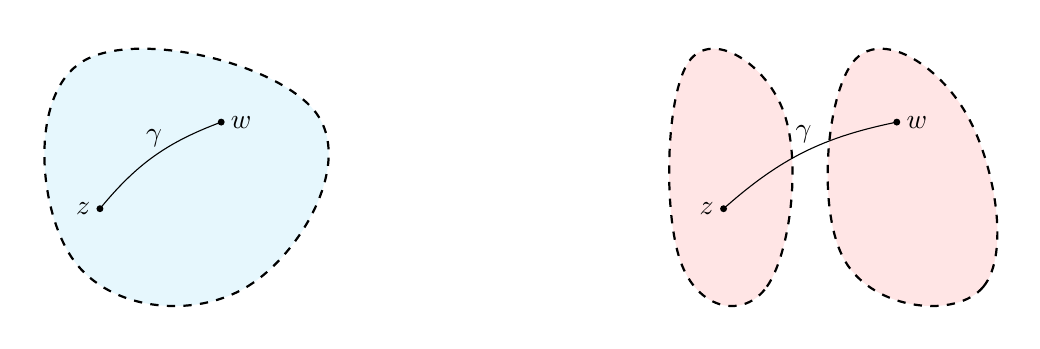
\begin{tikzpicture}[scale=1.1]
			\draw[dashed,thick, fill=cyan!10] plot[smooth cycle, tension=0.8] coordinates {(0,0) (2,-0.3) (2.8,1.7) (0.1,2.3)};
			\draw (0.3,0.6) node[left]{\(z\)} to[bend left=15] node[above]{\(\gamma\)} (1.7,1.6)node[right]{\(w\)};
			\fill[black] (0.3,0.6) circle (0.04);
			\fill[black] (1.7,1.6) circle (0.04);

			\begin{scope}[shift={(7,0)}]
				\draw[dashed,thick, fill=red!10] plot[smooth cycle, tension=0.8] coordinates {(0,0) (1,-0.3) (1.2,1.7) (0.1,2.3)};
				\draw[dashed,thick, fill=red!10] plot[smooth cycle, tension=0.8] coordinates {(1.9,0) (3.5,-0.3) (3.3,1.7) (2,2.3)};
				\draw (0.5,0.6) node[left]{\(z\)} to[bend left=15] node[above]{\(\gamma\)} (2.5,1.6)node[right]{\(w\)};
				\fill[black] (0.5,0.6) circle (0.04);
				\fill[black] (2.5,1.6) circle (0.04);
			\end{scope}
		\end{tikzpicture}
	\end{figure}

	As an example, the region shaded in blue on the left is path-connected, and therefore is a domain because for any two points in the region, we can connect them with a curve. While for the two-pieces subset on the right, if we take one point from each piece, then they cannot be connected by a curve completely within the subset. It is therefore not path connected and not a domain.

	\begin{rem}
		We make so many definitions above just to make sure that whenever we say `domain' in this chapter, it is a `single piece' of region without a boundary so that any point has a neighbourhood.
	\end{rem}



	\begin{defn}
		The \textit{complex derivative} of the function \(f:U\to\mathbb{C}\) at a point \(z=z_0\in U\) is
		\[f'(z_0)\coloneqq\lim_{z\to z_0}\frac{f(z)-f(z_0)}{z-z_0}\]
		if such a limit exists, and the function \(f(z)\) is said to be \textit{complex differentiable} at \(z=z_0\).
	\end{defn}
	\begin{rem}
		Complex differentiation satisfies the same formal rules (derivatives of sum, product, quotient, chain rule, and inverse functions) as the differentiation of functions of a real variable because they are defined by the same limit.
	\end{rem}
	\subsubsection{The Cauchy--Riemann Equations}
	Being complex differentiable is actually a very strict condition, as you will see later. It means that if we move by a small amount \(h\) in all possible directions in the complex plane, we must have
	\[f(z_0+h)=f(z_0)+h f'(z_0) + o(\abs{h})\,.\]
	This is stricter than viewing a complex function as a function defined on \(\mathbb{R}^2\) and ask it to be differentiable along \(x\) and \(y\) direction respectively. It must be differentiable, with the same derivative \(f'\) along all possible directions.

	This extra requirement can be captured by the Cauchy--Riemann equations.
	\begin{thm}[The Cauchy--Riemann equations]		
		\(f:U\to\mathbb{C}\) is differentiable at \(w=c+id\in U\) if and only if, writing \(f(x+iy)=u(x,y)+iv(x,y)\), \(u\) and \(v\) are real differentiable at \((c,d)\) and
		\[\left\{\begin{aligned}
			\pdv{u}{x}(c,d)&=\pdv{v}{y}(c,d)\\
			\pdv{v}{x}(c,d)&=-\pdv{u}{y}(c,d)\,.
		\end{aligned}\right.\]
	\end{thm}
	\begin{proof}
		\(f\) is differentiable at \(w=c+id\) with \(f'(w)=p+iq\)
		\begin{align*}
			&\iff\quad\lim_{z\to w}\frac{f(z)-f(w)-(z-w)(p+iq)}{z-w}=0\\
			&\iff\quad\lim_{z\to w}\frac{f(z)-f(w)-(z-w)(p+iq)}{\abs{z-w}}=0\,.
		\end{align*}
		Writing \(f=u+iv\) and evaluating the real and imaginary parts, this holds
		\[\iff\quad\left\{\begin{aligned}
			&\lim_{(x,y)\to(c,d)}\frac{u(x,y)-u(c,d)-[p(x-c)-q(y-d)]}{\sqrt{(x-c)^2+(y-d)^2}}=0\\
			&\lim_{(x,y)\to(c,d)}\frac{v(x,y)-v(c,d)-[q(x-c)+p(y-d)]}{\sqrt{(x-c)^2+(y-d)^2}}=0\,.
		\end{aligned}\right.\]
		Therefore, \(f\) is differentiable at \(w\) with derivative \(f'(w)=p+iq\) if and only if \(u,v\) are differentiable at \((c,d)\) with \(\grad u(c,d)=(p,-q)\) and \(\grad v(c,d) = (q,p)\).\qed
	\end{proof}

	\subsubsection{Holomorphic Functions}
	\begin{defn}
		A function \(f:U\to\mathbb{C}\) is \textit{holomorphic} at \(z_0\in U\) if there exists \(\epsilon>0\) such that \(f\) is differentiable for all \(z\in D(z_0,\epsilon)\). \(f\) is \textit{holomorphic on \(U\)} if it is differentiable at all \(z_0\in U\). The function is \textit{entire} if it is holomorphic in the whole complex plane.
	\end{defn}
	\begin{rem}
		To be holomorphic at some point, the function must be differentiable on a small neighbourhood of that point.
		
		The existence of a complex derivative in a neighbourhood is a very strong condition: it implies that a holomorphic function is infinitely differentiable.
	\end{rem}
	\begin{prop}
		Let \(f=u+iv:U\to \mathbb{C}\). Suppose that the functions \(u\), \(v\) have continuous partial derivatives everywhere on \(U\) and that they satisfy the Cauchy--Riemann equations, then \(f\) is holomorphic on \(U\).
	\end{prop}
	\begin{ex}
		Entire functions:
		\begin{enumerate}[topsep=0pt]
			\item \(f(z)=c\), where \(c\in\mathbb{C}\).
			\item \(f(z)=z\).
			\item \(f(z)=\exp(z)\).
			\item \(f(z)=z^n\), where \(n\in\mathbb{N}_0\).
		\end{enumerate}
	\end{ex}
	\textit{Property:} Sums, products and compositions of holomorphic functions are also holomorphic.
	
	\begin{ex}
		Non-holomorphic functions:
		\begin{enumerate}[topsep=0pt]
			\item \(f(z)=\Re z\).
			\item \(f(z)=z^*\).
			\item \(f(z)=\abs{z}\).
			\item \(f(z)=\abs{z}^2\).
		\end{enumerate}
	\end{ex}
	\begin{rem}
		In the last case, the Cauchy--Riemann equations are satisfied only at \(x=y=0\) and we can say that \(f'(0)=0\). However, \(f(z)\) is not holomorphic even at \(z=0\) because it is not differentiable throughout any neighbourhood \(\abs{z}<\epsilon\) of \(0\).
	\end{rem}
	\begin{defn}
		Many complex functions are holomorphic everywhere in the complex plane except at some isolated points, which are called the \textit{singular points} or \textit{singularities} of the function.
	\end{defn}
	\begin{ex}
		\(f(z)=z^c\), where \(c\in\mathbb{C}\), is holomorphic except at \(z=0\). (Strictly speaking for non-integer \(c\) we need a branch choice, so \(z^c\) is holomorphic on any simply connected domain avoiding the branch cut and \(0\).)
	\end{ex}
	\subsubsection{Consequences of the Cauchy--Riemann Equations}
	If we know the real part of a holomorphic function in some region, we can find its imaginary part (or vice versa) up to an additive constant by integrating the Cauchy--Riemann equations.
	\begin{prop}
		The real and imaginary parts of a holomorphic function satisfy Laplace's equation, i.e. \(u\) and \(v\) are \textit{harmonic functions}.
	\end{prop}
	\begin{proof}
		\begin{align*}
			\pdv[2]{u}{x}+\pdv[2]{u}{y}&=\pdv{x}\qty(\pdv{u}{x})+\pdv{y}\qty(\pdv{u}{y})\\
			&=\pdv{x}\qty(\pdv{v}{y})+\pdv{y}\qty(-\pdv{u}{x})\\
			&=0\,.
		\end{align*}
		Similarly, \(\laplacian v=0\).\qed
	\end{proof}
	\begin{prop}
		The curves of constant \(u\) and those of constant \(v\) are orthogonal. They are said to be \textit{conjugate harmonic functions}.
	\end{prop}
	\begin{proof}
		Using the Cauchy--Riemann equations, we have
		\begin{align*}
			\grad u\vdot\grad v&=\pdv{u}{x}\pdv{v}{x}+\pdv{u}{y}\pdv{v}{y}\\
			&=\pdv{v}{y}\pdv{v}{x}-\pdv{v}{x}\pdv{v}{y}\\
			&=0\,.
		\end{align*}\qed
	\end{proof}
	\begin{rem}
		Since \(u\) and \(v\) satisfy Laplace's equation, which is an elliptic PDE, it is guaranteed that \(u\) and \(v\) are smooth (and in fact analytic). This is a result of the elliptic regularity theorem.

		This is a (quite convoluted) way to prove that a holomorphic complex function is always smooth.
	\end{rem}
	\begin{thm}[Elliptic regularity theorem]
		For a differential equation
		\[\mathcal{L}\psi(\vb{x})=f(\vb{x})\,,\]
		where \(\mathcal{L}\) is an elliptic differential operator, if \(f\) is infinitely differentiable, then \(\psi\) is also infinitely differentiable.	
	\end{thm}
	
	\subsection{Power Series of a Complex Variable}
	\subsubsection{Convergence of Power Series}
	A complex power series about \(z=z_0\) has the form
	\[f(z)=\sum_{r=0}^{\infty}a_r (z-z_0)^r\text{ where }a_r\in\mathbb{C}\,.\]

	Many of the tests of convergence for real series can be generalised for complex series. Note that if the sum of the absolute values of a complex series converges, then so does the series. Hence if \(\sum \abs{a_r(z-z_0)^r}\) converges, so does \(\sum a_r (z-z_0)^r\).
	\begin{lem}\label[lem]{roclem}
		If the power series converges for \(z=z_1\), then the series converges absolutely for all \(z\) such that \(\abs{z-z_0}<\abs{z_1-z_0}\).
	\end{lem}
	\begin{proof}
		Since \(\sum a_r(z_1-z_0)^r\) converges, then from the necessary condition for convergence,
		\[\lim_{r\to\infty}a_r(z_1-z_0)^r=0\,.\]
		Hence for a given \(\epsilon\) there exists \(N=N(\epsilon)\) such that if \(r>N\) then
		\[\abs{a_r(z_1-z_0)}<\epsilon\,.\]
		Thus for \(r>N\),
		\begin{align*}
			\abs{a_r(z-z_0)^r}&=\abs{a_r(z_1-z_0)^r}\abs{\frac{z-z_0}{z_1-z_0}}^r\\
			&<\epsilon\varrho^r\,,\quad\text{where }\varrho=\abs{\frac{z-z_0}{z_1-z_0}}\,.
		\end{align*}
		Hence, by comparison with a geometric series, \(\sum a_r(z-z_0)^r\) converges for \(\varrho<1\), i.e. \(\abs{z-z_0}<\abs{z_1-z_0}\).\qed
	\end{proof}
	\begin{cor}
		If the power series diverges for \(z=z_1\) then it diverges for all \(\abs{z-z_0}>\abs{z_1-z_0}\).
	\end{cor}
	\begin{proof}
		This can be proven by contradiction. If the series converges for the sum \(z_2\) such that \(\abs{z_2-z_0}>\abs{z_1-z_0}\), then the series would converge for \(z=z_1\); this is a contradiction.\qed
	\end{proof}
	\begin{defn}
		Let \(c_n\) be a sequence of complex numbers. There must exist a unique real number \(R\in[0,\infty]\) such that the power series \(\sum c_n(z-z_0)^n\)
		\begin{itemize}[topsep=0pt]
			\item converges absolutely if \(0<\abs{z-z_0}<R\),
			\item diverges if \(\abs{z-z_0}>R\).
		\end{itemize}
		This \(R\) is called the \textit{radius of convergence}.
	\end{defn}
	\begin{proof}
		Trivial by \cref{roclem} and its corollary.\qed
	\end{proof}
	\begin{rem}
		On the circle of convergence, the series may either converge or diverge.
	\end{rem}
	\begin{cor}
		Let the complex power series \(\sum c_n(z-z_0)^n\) have a radius of convergence \(R>0\). Let \(0<r<R\), then the power series converges uniformly on \(D(z_0,r)\).
	\end{cor}
	\begin{proof}
		We know that \(\sum\abs{c_n}r^n\) is convergent. If \(\abs{z-z_0}\le r\), then
		\[\abs{c_n(z-z_0)^n}\le\abs{c_n}r^n\,.\]
		So the result follows from the Weierstrass M-test by taking \(M_n=\abs{c_n}r^n\).\qed
	\end{proof}
	\begin{rem}
		This can be seen as the uniform convergence of a geometric progression.
	\end{rem}
	\subsubsection{Determination of the Radius of Convergence}
	Without loss of generality take \(z_0=0\), so that the power series becomes
	\[f(z)=\sum_{r=0}^{\infty}u_r=\sum_{r=0}^{\infty}a_rz^r\,.\]
	\begin{prop}
		If the limit exists, then
		\[\lim_{r\to\infty}\abs{\frac{a_{r+1}}{a_r}}=\frac{1}{R}\,.\]
	\end{prop}
	\begin{proof}
		For the series to converge, we must have
		\[\lim_{r\to\infty}\abs{\frac{u_{r+1}}{u_r}}=\lim_{r\to\infty}\abs{\frac{a_{r+1}}{a_r}}\abs{z}<1\,.\]
		Therefore by the D'Alembert ratio test, the power series
		\[\text{converges if}\quad\frac{1}{\abs{z}}>\lim_{r\to\infty}\abs{\frac{u_{r+1}}{u_r}}\quad\text{and diverges if}\quad\frac{1}{\abs{z}}<\lim_{r\to\infty}\abs{\frac{u_{r+1}}{u_r}}\,.\]\qed
	\end{proof}
	\begin{prop}
		If the limit exists, then
		\[\lim_{r\to\infty}\abs{a_r}^{\frac{1}{r}}=\frac{1}{R}\,.\]
	\end{prop}
	\begin{proof}
		For the series to converge, we must have
		\[\lim_{r\to\infty}\abs{u_r}^{\frac{1}{r}}=\lim_{r\to\infty}\abs{a_r}^{\frac{1}{r}}\abs{z}<1\]
		by Cauchy's test.\qed
	\end{proof}
	\subsubsection{Holomorphicity of Analytic Functions (Non-examinable)}
	\begin{thm}\label{anahol}
		Let \(f(z)=\sum c_n(z-z_0)^n\) be a complex power series with radius of convergence \(R>0\), then
		\begin{enumerate}[topsep=0pt]
			\item \(f\) is holomorphic on \(D(z_0,R)\);
			\item its derivative is given by the series
			\[\sum_{n=0}^{\infty}nc_n(z-z_0)^{n-1}\,,\]
			which also has a radius of convergence \(R\);
			\item \(f\) has derivatives of all orders on \(D(z_0,R)\) and \(f^{(n)}(z_0)=n!c_n\).
		\end{enumerate}
	\end{thm}
	\begin{proof}
		We will assume wlog that \(z_0=0\). Consider the function
		\[\sum_{n=1}^{\infty}nc_nz^{n-1}\,.\]
		Since \(\abs{nc_n}\ge\abs{c_n}\), this series has radius of convergence \(R'\le R\). If \(0<R_1<R\), then for \(\abs{z}<R_1\), we have
		\[\abs{nc_nz^{n-1}}<nc_nR_1^{n-1}\frac{\abs{z}^{n-1}}{R_1^{n-1}}\,,\]
		so since \(n\frac{\abs{z}^{n-1}}{R_1^{n-1}}\to 0\) as \(n\to\infty\), for suitably large \(n\), \(\abs{c_n}R_1^{n-1}\) provides an upper bound for \(\abs{nc_nz^{n-1}}\). By the Weierstrass M-test, the series converges absolutely and uniformly on \(0<\abs{z-z_0}<R_1\), so the radius of convergence of this series is \(R\).

		Consider
		\begin{align}
			\frac{f(z)-f(w)}{z-w}&=\sum_{n=0}^{\infty}c_n\frac{z^n-w^n}{z-w}\nonumber\\
			&=\lim_{N\to\infty}\sum_{n=0}^{N}c_n\qty[\sum_{j=0}^{n-1}z_jw^{n-1-j}]\,. \tag{\(*\)}
		\end{align}
		For \(\abs{z},\abs{w}<r<R\), we have
		\[\abs{c_n\qty[\sum_{j=0}^{n-1}z_jw^{n-1-j}]}<\abs{c_n}nr^{n-1}\,,\]
		so \((*)\) converges uniformly on \(\abs{z},\abs{w}<r\), so the series has a continuous limit. We call it \(g(z,w)\). When \(z=w\),
		\[g(z,z)=\sum_{n=0}^{N}c_nnz^{n-1}\,.\]
		Therefore, \(f\) is differentiable with this derivative. This proves (i), (ii). (iii) is induction.\qed
	\end{proof}

	\subsection{Contour Integration}
	\begin{defn}
		A path (curve) \(\gamma:[a,b]\to\mathbb{C}\) is \textit{closed} if \(\gamma(a)=\gamma(b)\), and is \textit{simple} if \(\gamma\) is injective, possibly except at endpoints.
	\end{defn}
	This means that a simple path never crosses itself.
	\begin{defn}
		A \textit{contour} is a simple piecewise differentiable path.
	\end{defn}
	\begin{defn}
		Let \(f:U\to\mathbb{C}\) be a continuous complex function and \(\gamma:[a,b]\to U\) be a contour. The \textit{contour integral} of \(f\) along \(\gamma\) is
		\[\int_\gamma f(z)\dd{z}=\int_{a}^{b}f(\gamma(t))\gamma'(t)\dd{t}\,.\]
	\end{defn}
	\begin{ex}
		Consider the integral
		\[\int_\gamma \frac{1}{z}\dd{z}\]
		from \(z=-1\) to \(z=1\) along paths around half the unit circle (i). clockwise; (ii). anticlockwise. Making the substitution \(z=e^{i\theta}\), \(\dd{z}=ie^{i\theta}\), we have
		\[I_1=\int_{\gamma_1}\frac{1}{z}\dd{z}=\int_{\pi}^{0}\frac{ie^{i\theta}}{e^{i\theta}}\dd{\theta}=\int_{\pi}^{0}i\dd{\theta}=-i\pi\,,\]
		\[I_2=\int_{\gamma_2}\frac{1}{z}\dd{z}=\int_{\pi}^{2\pi}i\dd{\theta}=i\pi\,.\]
	\end{ex}
	\begin{rem}
		The result of a contour integration may depend on the contour.
	\end{rem}
	\begin{prop}
		Basic properties of contour integration:
		\begin{enumerate}[topsep=0pt]
			\item \textit{Linearity.}
			\[\int_\gamma c_1f_1(z)+c_2f_2(z)\dd{z}=c_1\int_\gamma f_1(z)\dd{z}+c_2\int_\gamma f_2(z)\dd{z}\,.\]
			\item \textit{Additivity.} If \(\gamma_1\) is a contour from \(z=a\) to \(z=b\), \(\gamma_2\) is a contour from \(z=b\) to \(z=c\), and \(\gamma\) is \(\gamma_1\) followed by \(\gamma_2\), then
			\[\int_\gamma f(z)\dd{z}=\int_{\gamma_1}f(z)\dd{z}+\int_{\gamma_2}f(z)\dd{z}\,.\]
			\item \textit{Inverse path.} If \(\gamma_+\) is a contour from \(\alpha\) to \(\beta\), and \(\gamma_-\) is the contour in reverse, then
			\[\int_{\gamma_+}f(z)\dd{z}=-\int_{\gamma_-}f(z)\dd{z}\,.\]
			\item \textit{Reparameterisation.} If \(\gamma:[a,b]\to U\) is a contour, \(\phi:[a',b']\to[a,b]\in C^1\) with \(\phi(a')=a\) and \(\phi(b')=b\) so that \(\delta=\gamma\circ\phi:[a',b']\to U\) is a different parameterisation of the same curve, then
			\[\int_\gamma f(z)\dd{z}=\int_\delta f(z)\dd{z}\,.\]
		\end{enumerate}
	\end{prop}
	\begin{lem}[ML estimation lemma]\label[lem]{estlem}
		If a contour \(\gamma\) has length \(L\), then
		\[\abs{\int_\gamma f(z)\dd{z}}\le L\sup\limits_{z\in\gamma}\abs{f(z)}\,.\]
	\end{lem}
	\begin{thm}[`Fundamental theorem of calculus']\label{contourftm}
		If \(F:U\to\mathbb{C}\) is holomorphic with a continuous derivative and \(\gamma:[a,b]\to U\) is a curve, then
		\[\int_\gamma F'(z)\dd{z}=F(\gamma(b))-F(\gamma(a))\,.\]
	\end{thm}
	\begin{proof}
		\[\int_\gamma F'(z)\dd{z}=\int_{a}^{b}F'(\gamma(t))\gamma'(t)\dd{t}=\int_{a}^{b}\dv{t}\qty(F(\gamma(t)))=[F(\gamma(t))]_a^b\,.\]\qed
	\end{proof}
	\subsection{Cauchy--Goursat Theorem}
	\begin{defn}
		A subset \(U\subseteq \mathbb{C}\) is \textit{simply connected} if it is path-connected and any loop \(\gamma:S^1\to U\) path can be continuously contracted to a point: for any \(\gamma\), there exists an extended continuous map \(\hat{\gamma}:D^2\to U\) such that \(\hat{\gamma}|_{S_1}=\gamma\). Here, \(S^1\) and \(D^2\) denote the unit circle and closed unit disk respectively.
	\end{defn}
	\begin{rem}
		A simply connected domain has no `hole' in it.
	\end{rem}
	\begin{thm}[Cauchy--Goursat theorem]\label{cauthm}	
		If a function \(f\) is holomorphic and has continuous partial derivatives in a simply connected domain \(U\), then for any closed contour \(\gamma\) in \(U\),
		\[\oint_\gamma f(z)\dd{z}=0\,.\]
	\end{thm}
	\begin{proof}
		Green's theorem states that, for a vector field \(\vb{p}=(p,q)\),
		\[\oint_\gamma(p\dd{x}+q\dd{y})=\int_\Omega\qty(\pdv{q}{x}-\pdv{p}{y})\dd{x}\dd{y}\,,\]
		where \(\Omega\) is the simply connected region bounded by a simple closed curve \(\gamma\). Hence, by expanding into real and imaginary parts and using the Cauchy--Riemann equations,
		\begin{align*}
			\oint_\gamma f(z)\dd{z}&=\oint_\gamma(u+iv)(\dd{x}+i\dd{y})\\
			&=\oint_\gamma(u\dd{x}-v\dd{y})+i\oint_\gamma(v\dd{x}+u\dd{y})\\
			&=\int_\Omega\qty(-\pdv{u}{y}-\pdv{v}{x})\dd{x}\dd{y}+i\int_\Omega\qty(-\pdv{v}{y}+\pdv{u}{x})\dd{x}\dd{y}=0\,.
		\end{align*}\qed
	\end{proof}
	\begin{rem}
		This is a weaker version of this theorem proven by Cauchy. It requires \(f\) to be holomorphic and have continuous partial derivatives. A stronger version of this theorem, proven by Goursat, removes the need for partial-derivative continuity.
	\end{rem}
	\subsubsection{Deforming Contours}
	\begin{prop}
		Let \(\gamma_1\) and \(\gamma_2\) be two different contours both from \(\alpha\) to \(\beta\). If \(f(z)\) is a function that is holomorphic on both contours and inside the region bounded by the contours, then
		\[\int_{\gamma_1}f(z)\dd{z}=\int_{\gamma_2}f(z)\dd{z}\,.\]
	\end{prop}
	\begin{proof}
		Consider the closed curve \(\gamma=\gamma_1-\gamma_2\). It follows from Cauchy's theorem that
		\[\oint_\gamma f(z)\dd{z}=\int_{\gamma_1}f(z)\dd{z}-\int_{\gamma_2}f(z)\dd{z}=0\,.\]
		The proposition hence follows.\qed
	\end{proof}
	\begin{cor}
		We can deform a contour without changing the value of the integral as long as we do not move the contour across a singularity.
	\end{cor}
	\begin{cor}
		We can deform a closed contour if we are not passing it through any singularity.
	\end{cor}
	\begin{rem}
		This concept of continuously deforming a contour is formally known as a \textit{homotopy} in algebraic topology.
	\end{rem}
	This is possible even if the contour have (the same) singular points enclosed before and after deformation. Consider two closed contours \(\gamma_1\) and \(\gamma_2\) shown below. Let \(f(z)\) be holomorphic within the region bounded between \(\gamma_1\) and \(\gamma_2\), but has singularities enclosed by \(\gamma_2\). Consider cutting off a small piece of each contour and joining them together by two bridges \(\gamma_\epsilon\) and \(\gamma_\epsilon'\) to form a closed contour \(\Gamma\).

	We have \(\Gamma=\gamma_1'-\gamma_2'+\gamma_\epsilon+\gamma_\epsilon'\). Since \(f(z)\) is holomorphic in the region bounded by \(\Gamma\) by assumption, we have
	\[\int_\Gamma f(z)\dd{z}=0\,.\]
	If we take the limit such that the width of the cut \(\to 0\), we have \(\gamma_1'\to\gamma\), \(\gamma_2'\to\gamma_2\) and \(\gamma_\epsilon'\to\gamma_\epsilon\). Therefore,
	\[\int_\Gamma f(z)\dd{z}\to\int_{\gamma_1}f(z)\dd{z}-\int_{\gamma_2}f(z)\dd{z}=0\,,\]
	so the integral along two closed contours enclosing the same singularities is the same.

	\begin{figure}[ht!]
		\centering
		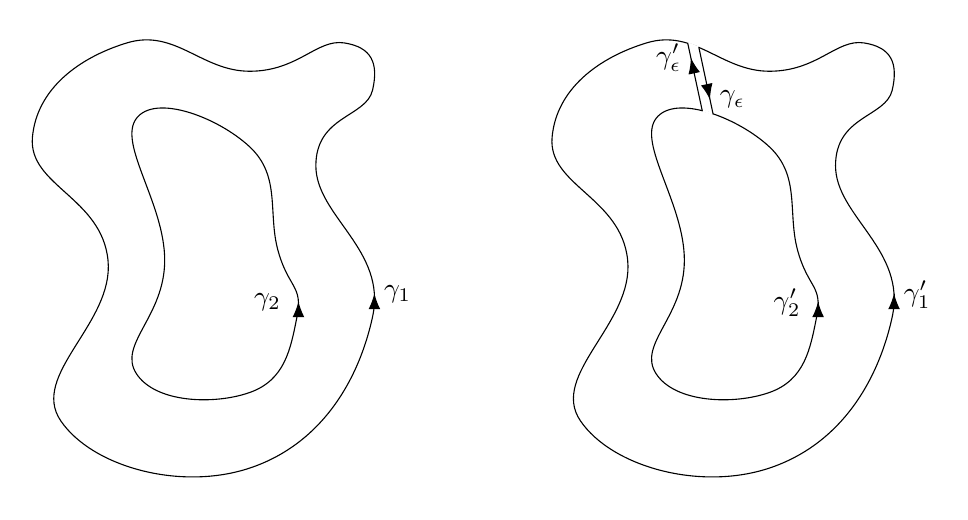
\begin{tikzpicture}[>=latex,scale=0.12]
			\coordinate (A) at (3,-9);
			\coordinate (B) at (-3,7);
			\coordinate (C) at (3,15);
			\coordinate (D) at (0,20);
			\coordinate (E) at (-10,17);
			\coordinate (F) at (-23,20);
			\coordinate (G) at (-33,10);
			\coordinate (H) at (-25,-3);
			\coordinate (I) at (-30,-20);
			\coordinate (J) at (-10,-25);

			\coordinate (K) at (-7,-2);
			\coordinate (L) at (-10,9);
			\coordinate (M) at (-22,12);
			\coordinate (N) at (-19,-3);
			\coordinate (O) at (-22,-15);
			\coordinate (P) at (-10,-17);
			\coordinate (Q) at (-5,-9);

			\draw[
				postaction={decorate},
				decoration={
					markings,
					mark=at position 0.9 with \coordinate(M1);,
				}
			]
			plot [smooth cycle, tension=0.8]
			coordinates { (A) (B) (C) (D) (E) (F) (G) (H) (I) (J) };

			\node at (M1) [right] {\(\gamma_1\)};
			\draw[-{Latex[length=2mm]}] (M1)--+(90:0.1);

			\draw[
				postaction={decorate},
				decoration={
					markings,
					mark=at position 0.79 with \coordinate(M2);,
				}
			]
			plot [smooth cycle, tension=0.8]
			coordinates { (K) (L) (M) (N) (O) (P) (Q) };

			\node at (M2) [left=1mm] {\(\gamma_2\)};
			\draw[-{Latex[length=2mm]}] (M2)--+(90:0.1);
			
			\draw[
				postaction={decorate},
				decoration={
					markings,
					mark=at position 0.9 with \coordinate(M3);,
				}
			]
			plot [smooth cycle, tension=0.8] coordinates { ([xshift=55cm]A) ([xshift=55cm]B) ([xshift=55cm]C) ([xshift=55cm]D) ([xshift=55cm]E) ([xshift=55cm]F) ([xshift=55cm]G) ([xshift=55cm]H) ([xshift=55cm]I) ([xshift=55cm]J) };

			\node at (M3) [right] {\(\gamma_1'\)};
			\draw[-{Latex[length=2mm]}] (M3)--+(90:0.1);

			\draw[
				postaction={decorate},
				decoration={
					markings,
					mark=at position 0.79 with \coordinate(M4);,
				}
			]
			plot [smooth cycle, tension=0.8] coordinates { ([xshift=55cm]K) ([xshift=55cm]L) ([xshift=55cm]M) ([xshift=55cm]N) ([xshift=55cm]O) ([xshift=55cm]P) ([xshift=55cm]Q) };

			\node at (M4) [left=1mm] {\(\gamma_2'\)};
			\draw[-{Latex[length=2mm]}] (M4)--+(90:0.1);

			\draw[white,thick] (38,12.81)--(38.9,12.54)--(37.4,19.55)--(36.5,19.9)--(38,12.81);
			
			\draw[
				postaction={decorate},
				decoration={
					markings,
					mark=at position 0.78 with \arrow{Latex[length=2mm]},
				}
			]
			(37.53,19.55)--(39.05,12.43)node[pos=0.78,right]{\(\gamma_\epsilon\)};

			\draw[
				postaction={decorate},
				decoration={
					markings,
					mark=at position 0.78 with \arrow{Latex[length=2mm]},
				}
			]
			(37.9,12.8)--(36.35,20)node[pos=0.78,left]{\(\gamma_\epsilon'\)};
		\end{tikzpicture}
	\end{figure}

	\begin{rem}
		This is connected with \cref{contourftm}. If we can find a function \(F(z)\) that is holomorphic in a simply connected domain \(U\) and \(F'(z)=f(z)\), then
		\[\int_{\gamma}f(z)\dd{z}=F(\gamma(b))-F(\gamma(a))\]
		for all \(\gamma:[a,b]\to U\). The integral is invariant.
	\end{rem}
	\subsection{Cauchy's Integral Formula}
	\begin{thm}[Cauchy's integral formula]
		If \(f(z)\) is holomorphic on a domain \(U\subseteq\mathbb{C}\), \(z_0\in U\), and \(\gamma\subset U\) is an arbitrary simple closed contour that encircles \(z_0\) counter-clockwise. We have Cauchy's integral formula
		\[f(z_0)=\frac{1}{2\pi i}\oint_\gamma\frac{f(z)}{z-z_0}\dd{z}\,.\]
	\end{thm}
	\begin{proof}
		\(\frac{f(z)}{z-z_0}\) is holomorphic everywhere except at \(z=z_0\). Therefore, we can deform \(\gamma\) to an arbitrarily small contour, say a circle of radius \(\epsilon\) around \(z_0\), \(\gamma_\epsilon\) contained completely within \(\gamma\). By substituting \(z=z_0+\epsilon e^{i\theta}\), we have
		\begin{align*}
			\oint_\gamma\frac{f(z)}{z-z_0}\dd{z}&=\oint_{\gamma_\epsilon}\frac{f(z)}{z-z_0}\dd{z}\\
			&=\int_{0}^{2\pi}\frac{f(z_0+\epsilon e^{i\theta})}{\epsilon e^{i\theta}}i\epsilon e^{i\theta}\dd{\theta}\,.
		\end{align*}
		Take the limit \(\epsilon\to 0\), we have
		\begin{align*}
			\oint_\gamma\frac{f(z)}{z-z_0}\dd{z}&=i\lim_{\epsilon\to 0}\int_0^{2\pi}f(z_0+\epsilon e^{i\theta})\dd{\theta}\\
			&=i\int_{0}^{2\pi}f(z_0)\dd{\theta}=2\pi if(z_0)\,.
		\end{align*}\qed
	\end{proof}
	\begin{rems}
		\begin{itemize}[topsep=0pt]
			\item If we know \(f(z)\) on \(\gamma\), then from the Cauchy's formula, we know \(f(z)\) throughout the interior of \(\gamma\).
			\item Since the real and imaginary parts of an analytic function, \(u\) and \(v\), satisfy Laplace's equation, this statement is equivalent to the uniqueness of the solutions to Laplace's equation with Dirichlet boundary conditions (\cref{uniquepoi}).
			
			In particular, if we specify \(u\) and \(v\) on \(\gamma\), then there is a unique solution for \(u\) and \(v\) inside \(\gamma\). This is equivalent to the integral solution of Poisson's equation that we will see later (\cref{intpoi}).
		\end{itemize}
	\end{rems}
	\begin{cor}[The mean-value property]
		If \(f:D(z_0,r)\to\mathbb{C}\) is holomorphic, then
		\[f(z_0)=\int_{0}^{1}f(z_0+re^{2\pi it})\dd{t}\,.\]
	\end{cor}
	\begin{proof}
		Change the variable \(\theta=2\pi t\) in the above proof and done.\qed
	\end{proof}
	\begin{rem}
		\(f(w)\) equals the average value of \(f\) on any circle with centre \(w\).
	\end{rem}
	\begin{thm}[Liouville's theorem]		
		Every bounded entire function must be constant.
	\end{thm}
	\begin{proof}
		Let \(f:\mathbb{C}\to\mathbb{C}\) be an entire function such that \(\abs{f}<M\). For any \(w\in\mathbb{C}\), let \(R>\abs{w}\),
		\begin{align*}
			\abs{f(w)-f(0)}&=\frac{1}{2\pi}\abs{\int_{\abs{z}=R}f(z)\qty(\frac{1}{z-w}-\frac{1}{z})\dd{z}}\\
			&=\frac{1}{2\pi}\abs{\int_{\abs{z}=R}\frac{wf(z)}{z(z-w)}\dd{z}}\\
			&\le\frac{1}{2\pi}\times 2\pi R\times\frac{M\abs{w}}{R(R-\abs{w})}\to 0\text{ as }R\to\infty\,,
		\end{align*}
		so \(f(w)=f(0)\) by Cauchy's formula and ML estimation lemma. \qed
	\end{proof}
	\subsection{Taylor Expansion}
	\begin{thm}[Complex Taylor expansion]
		Let \(f:D(z_0,r)\to\mathbb{C}\) be holomorphic, then \(f\) has a convergent power series representation on \(D(z_0,r)\):
		\[f(z)=\sum_{n=0}^{\infty}c_n(z-z_0)^n\,,\]
		where
		\[c_n=\frac{f^{(n)}(z_0)}{n!}=\frac{1}{2\pi i}\int_{\abs{z-z_0}=\rho}\frac{f(z)}{(z-z_0)^{n+1}}\dd{z}\]
		for arbitrary \(0<\rho<r\).
	\end{thm}
	\begin{proof}[Non-examinable]
		Let \(\abs{w-z_0}<\rho<r\). Using the geometric series, we have
		\[\frac{1}{z-w}=\frac{1}{(z-z_0)\qty(1-\frac{w-z_0}{z-z_0})}=\sum_{n=0}^{\infty}\frac{(w-z_0)^n}{(z-z_0)^{n+1}}\]
		which converges uniformly for \(\abs{z-z_0}=\rho\). By the Cauchy integral formula,
		\begin{align*}
			f(w)&=\frac{1}{2\pi i}\int_{\abs{z-z_0}=\rho}\frac{f(z)}{z-w}\dd{z}\\
			&=\frac{1}{2\pi i}\int_{\abs{z-z_0}=\rho}f(z)\sum_{n=0}^{\infty}\frac{(w-z_0)^n}{(z-z_0)^{n+1}}\dd{z}\\
			&=\sum_{n=0}^{\infty}\qty(\frac{1}{2\pi i}\int_{\abs{z-z_0}=\rho}f(z)\frac{1}{(z-z_0)^{n+1}}\dd{z})(w-z_0)^n\,,
		\end{align*}
		where the interchange of integration and summation is justified by the uniform convergence of the geometric progression. So \(f\) has a convergent power series representation on \(D(z_0,\rho)\) for any \(\rho<r\).
		
		Differentiate the Cauchy's integral formula \(n\) times to get
		\[f(z_0)^{(n)}=\frac{n!}{2\pi i}\int_{\abs{z-z_0}=\rho}\frac{f(z)}{(z-z_0)^{n+1}}\dd{z}\,,\]
		so the coefficients of the power series are \(f^{(n)}(z_0)/n!\).\qed
	\end{proof}
	\begin{cor}
		If \(f:U\to \mathbb{C}\) is holomorphic then its derivatives of all orders exist and are holomorphic.
	\end{cor}
	\begin{defn}
		A function \(f:U\to\mathbb{C}\) is said to be \textit{analytic} if every \(z_0\in U\), \(f\) can be represented by a convergent power series on some \(D(z_0,r)\subset U\).
	\end{defn}
	\begin{thm}
		For a complex function \(f:U\to\mathbb{C}\), holomorphic \(\iff\) analytic \(\implies\) infinitely differentiable.
	\end{thm}
	Note that `smooth' in complex analysis means infinitely differentiable in \(\mathbb{R}^2\) sense, not infinitely complex differentiable, so smoothness does not imply holomorphicity (e.g. \(f(z)=z^*\)).
	\begin{proof}
		Analytic \(\implies\) holomorphic by \cref{anahol}. Holomorphic \(\implies\) infinitely differentiable and analytic by the previous theorem.\qed
	\end{proof}
	\begin{rem}
		This is not the case in real analysis. A once differentiable real function is far from being infinitely differentiable. Even if a function is infinitely differentiable in some interval, it can be nowhere analytic. The Taylor series may have a radius of convergence of zero, or the function defined by its Taylor series fails to converge to \(f\).
	\end{rem}

	From now on, we shall use the terms `holomorphic' and `analytic' interchangeably.

	\subsection{Analytic Continuation (Non-examinable)}
	The fact that holomorphic functions are analytic has an interesting and important consequence: a holomorphic function on a domain \(U\) is determined by its restriction to a subdomain in \(U\).
	\begin{defn}
		Let \(U'\subset U\) be domains and \(f:U'\to\mathbb{C}\) be analytic. A function \(g(z):U\to\mathbb{C}\) is called the \textit{analytic continuation} of \(f\) if it is analytic and \(f(z)=g(z)\) for all \(z\in U'\)
	\end{defn}

	\begin{thm}
		The analytic continuation of a function is unique (if exists).
	\end{thm}
	\begin{proof}
		Let \(g_1,g_2:U\to\mathbb{C}\) be analytic continuations of \(f:U'\to\mathbb{C}\) to \(U\). Then \(h=g_1-g_2:U\to\mathbb{C}\) is analytic and \(h(z)=0\) on \(U'\). It suffices to show that \(h\) is identically zero on \(U\). Define
		\begin{align*}
			U_0&=\{w\in U\mid h\text{ is identically 0 on some open disk }D(w,r)\}\\
			U_1&=\{w\in U\mid h^{(n)}(w)\ne 0\text{ for some }n>0\}\,.
		\end{align*}
		Then since \(h\) has a convergent power series expansion about each point \(w\in U\), we see that \(U=U_0\cup U_1\) and \(U_0\cap U_1=\varnothing\). Moreover, both \(U_0\) and \(U_1\) are open subsets of \(\mathbb{C}\). So as \(U\) is connected, one of \(U_i\) is empty, and as \(U_0\supset U'\ne\varnothing\) we must have \(U_1=\varnothing\), so \(U=U_0\) and \(h=0\) on all of \(U\).\qed
	\end{proof}

	\subsection{Singularities and the Laurent Expansion}
	\begin{thm}
		Let \(f\) be holomorphic on an annulus \(A=\{z\in\mathbb{C}\mid r<\abs{z-z_0}<R\}\), where \(0\le r<R\le\infty\). Then
		\begin{enumerate}[topsep=0pt]
			\item There is a unique convergent \textit{Laurent series expansion} on \(A\)
			\[f(z)=\sum_{n=-\infty}^{\infty}c_n(z-z_0)^n\,.\]
			\item For any \(\rho\in(r,R)\), the coefficient \(c_n\) of the Laurent series is given by
			\[c_n=\frac{1}{2\pi i}\int_{\abs{z-z_0}=\rho}\frac{f(z)}{(z-z_0)^{n+1}}\dd{z}\,.\]
			\item If \(r<\rho'\le\rho<R\), then the Laurent series converges uniformly on \(\{z\in\mathbb{C}\mid \rho'\le\abs{z-z_0}\le\rho\}\), and hence on any compact subdomain of \(A\).
		\end{enumerate}
	\end{thm}
	\begin{proof}[Non-examinable]
		For a given \(w\in A\), choose \(r<\rho_2<\abs{w-z_0}<\rho_1<R\) and consider the circular paths \(\gamma_1\), \(\gamma_2\), where \(\gamma_i\) is the circle \(\abs{z-z_0}=\rho_i\). Construct a path \(\Gamma\) by joining \(\gamma_1\) and \(\gamma_2\) together with two straight paths of width \(\epsilon\). By the Cauchy's integral formula and taking \(\epsilon\to 0\), we have
		\begin{align*}
			f(w)&=\frac{1}{2\pi i}\int_{\Gamma}\frac{f(z)}{z-w}\dd{z}\\
			&=\frac{1}{2\pi i}\int_{\gamma_1}\frac{f(z)}{z-w}\dd{z}-\frac{1}{2\pi i}\int_{\gamma_2}\frac{f(z)}{z-w}\dd{z}\\
			&\eqqcolon f_1(w)+f_2(w)\,.
		\end{align*}

		\begin{figure}
			\centering
			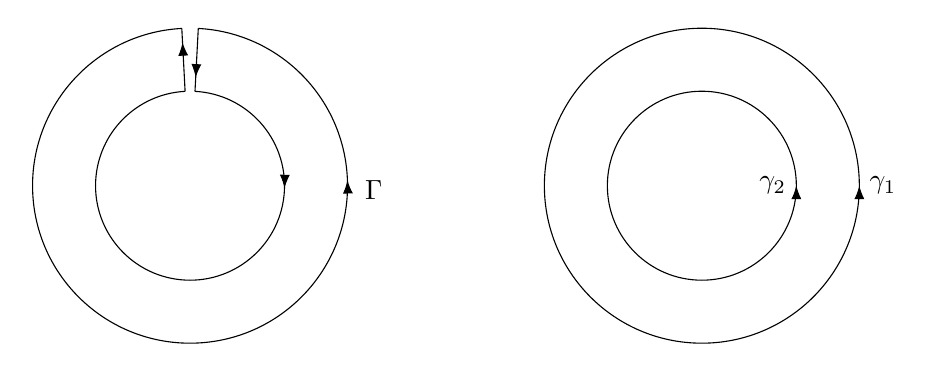
\begin{tikzpicture}
				\draw[
					postaction={decorate},
					decoration={
						markings,
						mark=at position 0.76 with \arrow{Latex[length=1.7mm]},
					}
				]
				(93:2) arc (93:447:2)node[pos=0.75,right=1mm]{\(\Gamma\)};

				\draw[
					postaction={decorate},
					decoration={
						markings,
						mark=at position 0.25 with \arrow{Latex[length=1.7mm]},
					}
				]
				(87:1.2) arc (447:93:1.2);

				\draw[
					postaction={decorate},
					decoration={
						markings,
						mark=at position 0.78 with \arrow{Latex[length=1.7mm]},
					}
				]
				(87:2)--(87:1.2);
				\draw[
					postaction={decorate},
					decoration={
						markings,
						mark=at position 0.78 with \arrow{Latex[length=1.7mm]},
					}
				]
				(93:1.2)--(93:2);

				\draw[
					postaction={decorate},
					decoration={
						markings,
						mark=at position 0 with \arrow{Latex[length=1.7mm]},
					}
				]
				(6.5,0) circle (2);

				\node at (8.8,0){\(\gamma_1\)};

				\draw[
					postaction={decorate},
					decoration={
						markings,
						mark=at position 0 with \arrow{Latex[length=1.7mm]},
					}
				]
				(6.5,0) circle (1.2);

				\node at (7.4,0){\(\gamma_2\)};
			\end{tikzpicture}
		\end{figure}

		For the first integral term \(f_1(w)\), expand as in the proof of the Taylor series to get \(f_1(w)=\sum_{n=0}^{\infty}c_n(w-z_0)^n\), where
		\[c_n=\frac{1}{2\pi i}\int_{\abs{z-z_0}=\rho_1}\frac{f(z)}{(z-z_0)^{n+1}}\dd{z}\,,\text{for all }n\ge 0\,.\]
		For the second integral term \(f_2(w)\), use the geometric series
		\[\frac{-1}{z-w}=\frac{\frac{1}{w-z_0}}{1-\frac{z-z_0}{w-z_0}}=\sum_{m=1}^{\infty}\frac{(z-z_0)^{m-1}}{(w-z_0)^m}\]
		which converges uniformly for \(\abs{z-z_0}=\rho_2\). This gives \(f_2(w)=\sum_{m=1}^{\infty}d_m(w-z_0)^{-m}\), where
		\[d_m=\frac{1}{2\pi i}\int_{\abs{z-z_0}=\rho_2}\frac{f(z)}{(z-z_0)^{-m+1}}\dd{z}\,\text{for all }m\ge 1\,.\]
		Combining these two results gives (i).

		To show (ii) and (iii), suppose that we have any convergent series \(\sum_{n=-\infty}^{\infty} c_n(z-z_0)^n\) on \(A\),  and let \(r<\rho'\le\rho<R\). Then the power series \(\sum_{n=0}^{\infty}c_n(z-z_0)^n\) must have radius of convergence \(\ge R\), so converges uniformly on \(\{\abs{z-z_0}\le\rho\}\). Likewise, let \(u=(z-z_0)^{-1}\), then the series \(\sum_{n=1}^{\infty}c_{-n}u^n\) must have a radius of convergence \(\ge\frac{1}{r}\), so converges uniformly on \(\{\abs{u}\le\frac{1}{\rho'}\}\). Therefore, the series \(\sum_{n=-\infty}^{\infty} c_n(z-z_0)^n\) converges uniformly on \(\{\rho'\le\abs{z-z_0}\le\rho\}\) and therefore in particular can be integrated term-by-term along any curve in this set; so
		\[\int_{\abs{z-z_0}=\rho}\frac{f(z)}{(z-z_0)^{m+1}}\dd{z}=\sum_{n=-\infty}^{\infty}c_n\int_{\abs{z-z_0}=\rho}(z-z_0)^{n-m-1}=2\pi i c_m\,.\]\qed
	\end{proof}
	\begin{defn}
		The \textit{zeros} of a holomorphic function \(f(z)\) are the points \(z=z_0\) where \(f(z_0)=0\). A zero is of \textit{order} \(k\) if the first non-zero term in the Taylor expansion of \(f(z)\) about \(z_0\) is \(c_k(z-z_0)^k\).
	\end{defn}
	\begin{defn}
		A \textit{singularity} of a function \(f\) is a point \(z=z_0\) where \(f\) is not holomorphic. If \(f\) has a singularity at \(z_0\), but \(f\) is holomorphic in a neighbourhood of \(z_0\) except at \(z_0\) itself, then \(z_0\) is an \textit{isolated singularity} of \(f\). If there exists no such neighbourhood, \(z_0\) is a non-isolated singularity.
	\end{defn}
	\begin{exs}
		\begin{enumerate}[topsep=0pt]
			\item \(f=\mathrm{cosech}\,z=\frac{1}{\sinh z}\) has isolated singularities at \(z=in\pi\), \(n\in\mathbb{Z}\) because \(\sinh x=0\) at these points.
			\item \(f=\mathrm{cosech}\,\frac{1}{z}\) has isolated singularities at \(z=\frac{1}{in\pi}\), \(n\in\mathbb{Z}\setminus\{0\}\). \(f\) also has a non-isolated singularity at \(z=0\); for any disk \(D(\epsilon,0)\) we can find a large enough \(n\) such that the disk contains another singularity at \(z=\frac{1}{in\pi}\).
		\end{enumerate}
	\end{exs}

	We shall usually be concerned with isolated singularities, for which \(f(z)\) is holomorphic on the punctured disk \(D(z_0,R)^{\cross}\coloneqq D(z_0,R)\setminus\{z_0\}\).
	\begin{defn}
		There are three possible behaviours of \(f\) with isolated singularities:
		\begin{enumerate}[topsep=0pt]
			\item If the first non-zero term in the Laurent series of \(f\) has \(n\ge 0\), then the Laurent series converges throughout the unpunctured disk \(D(z_0,R)\). We say \(f\) has a \textit{removable singularity} at \(z=z_0\).
			\item If there exists some finite \(k>0\) such that \(c_{-k}\ne 0\) but \(c_n=0\) for all \(n<-k\), then \(f\) has a \textit{pole of order \(k\)} at \(z=z_0\).
			\item Otherwise, if the Laurent series centred at \(z=z_0\) involves an infinite number of terms with \(n<0\), we say \(f\) has an \textit{essential singularity} at \(z=z_0\).
		\end{enumerate}
	\end{defn}
	\begin{exs}
		\begin{enumerate}[topsep=0pt]
			\item Removable singularity typically arises when \(f\) is given by some formula which is not well-defined at \(z=z_0\); for example, take \(z_0=0\) and \(f(z)=(e^z-1)/z\).
			\item An example of essential singularity is \(f(z)=e^{\frac{1}{z}}\) at \(z=0\).
			\[e^{\frac{1}{z}}=\sum_{n=0}^{\infty}\frac{1}{n!}\qty(\frac{1}{z})^n=\sum_{n=-\infty}^{0}\frac{1}{(-n)!}z^n\,.\]
		\end{enumerate}
	\end{exs}

	\begin{rem}
		The behaviour of a function near an essential singularity is remarkably complicated.
	\end{rem}
	\begin{thm}[Picard's theorem]		
		In any neighbourhood of an essential singularity, the function takes all possible complex values (possibly with one exception) at infinitely many points.
	\end{thm}
	\begin{ex}
		In the case of \(e^{\frac{1}{z}}\), the exceptional value 0 is never obtained.
	\end{ex}
	\begin{prop}
		\(f\) has a removable singularity at \(z=z_0\) if and only if
		\[\lim_{z\to z_0}(z-z_0)f(z)=0\,.\]
	\end{prop}
	\begin{proofskip}
		\begin{itemize}[topsep=0pt]
			\item[(\(\Rightarrow\))] Write
			\[(z-z_0)f(z)=\sum_{n=0}^{\infty}c_n(z-z_0)^{n+1}\]
			so it vanishes as \(z\to z_0\).
			\item[(\(\Leftarrow\))] Consider
			\[g(z)=\begin{cases}
				(z-z_0)^2f(z) & \text{if }z\ne z_0\\
				0 & \text{if }z=z_0\,.
			\end{cases}\]
			We see that \(g\) is holomorphic and \(g'(z_0)=0\) so
			\[g(z)=\sum_{n=2}^{\infty}c_n(z-z_0)^n\]
			\[f(z)=\sum_{n=0}^{\infty}c_{n+2}(z-z_0)^n\]
			and hence \(f\) has a removable singularity at \(z=z_0\).
		\end{itemize}\qed
	\end{proofskip}
	\begin{prop}
		\(f\) has a pole at \(z=z_0\) if and only if \(\abs{f(z)}\to\infty\) as \(z\to z_0\). Moreover, the following statements are equivalent:
		\begin{enumerate}[topsep=0pt]
			\item \(f\) has a pole of order \(k\) at \(z=z_0\).
			\item \(f=(z-a)^{-k}g(z)\), where \(g:D(z_0,R)\to\mathbb{C}\) is holomorphic and \(g(z_0)\ne 0\).
			\item \(f(z)=\frac{1}{h(z)}\), where \(h\) is holomorphic at \(z=z_0\) with a zero of order \(k\).
		\end{enumerate}
	\end{prop}
	\begin{proof}
		First, prove (i) \(\Leftrightarrow\) (ii). Given \(f\) with a pole, multiplying the Laurent series by \((z-z_0)^k\) gives a power series with a non-zero constant term, defining \(g\), and the converse is clear. The Taylor series for g multiplied with \((z-z_0)^{-k}\) gives the Laurent series for \(f\).
 		
		Next, (ii) \(\Leftrightarrow\) (iii). This is because \(g\) is holomorphic and non-zero \(z=z_0\) if and only if \(1/g\) is holomorphic and non-zero at \(z=z_0\).
		
		Suppose \(f\) has a pole at \(z=z_0\). Then by (ii) \(\abs{f}\to\infty\) as \(z\to z_0\). Conversely if \(\abs{f}\to\infty\) as \(z\to z_0\), then for some \(r>0\), \(f\) is non-zero for \(0 <\abs{z-z_0}<r\). Therefore \(1/f\) is holomorphic for \(0<\abs{z-z_0}<r\) and \(1/f\to 0\) as \(z\to z_0\). By the previous proposition, \(1/f\) has a removable singularity at \(z=z_0\). Thus there is a holomorphic \(h\) on \(D(z_0,r)\) with \(1/h = f\) for \(0<\abs{z-z_0}<r\). As \(1/f\to 0\) as \(z\to z_0\), \(h\) has a zero at \(z=z_0\).\qed
	\end{proof}
	\subsubsection{Meromorphic Functions}
	\begin{defn}
		Let \(U\) be a domain and \(S\subset U\) is a set of isolated points in \(U\), then a function \(f:U\setminus S\to\mathbb{C}\) with at worst poles (poles and removable singularities) at the points in \(S\) is said to be \textit{meromorphic}.
	\end{defn}
	\begin{rem}
		A function \(f\) meromorphic on \(U\) can be written as \(f=\frac{g}{h}\),
		where \(g\) and \(h\) are holomorphic on \(U\).
	\end{rem}

	\subsubsection{Behaviour at Infinity}
	We can examine the behaviour of a function \(f(z)\) as \(z\to\infty\) by defining a new variable \(\xi=\frac{1}{z}\) and a new function \(g(\xi)=f(z)\). The \(z=\infty\) maps to a single point \(\xi=0\), the point at infinity.
	\begin{exs}
		\begin{enumerate}[topsep=0pt]
			\item \(f(z)=e^z=e^{\frac{1}{\xi}}=g(\xi)\) has an essential singularity at \(z=\infty\).
			\item \(f(z)=z^2=\frac{1}{\xi^2}=g(\xi)\) has a double pole at \(z=\infty\).
			\item \(f(z)=e^{\frac{1}{z}}=e^\xi=g(\xi)\) is analytic at \(z=\infty\).
		\end{enumerate}
	\end{exs}
	\begin{rem}
		All entire functions \(f(z)\) have essential singularities at \(z=\infty\) unless they are polynomials, and all polynomials have poles at \(z=\infty\) unless they are constant.
	\end{rem}

	\newpage

	\section{Series Solutions of Ordinary Differential Equations}
	\subsection{Linear Independence and the Wronskian}
	\subsubsection{Linearly Independent Solutions}
	Consider homogeneous second-order linear ordinary differential equations of the form
	\begin{equation}\tag{\(\dagger\)}
		y''+p(x)y'+q(x)y=0\,.
	\end{equation}
	Recall that two solutions \(y_1\) and \(y_2\) are linearly independent if and only if
	\[\alpha y_1(x)+\beta y_2(x)=0\implies \alpha=\beta=0\,.\]
	If \(y_1(x)\) and \(y_2(x)\) are linearly independent solutions, then the general solution of the ODE is given by
	\[y(x)=\alpha y_1(x)+\beta y_2(x)\,,\]
	where \(\alpha\) and \(\beta\) are arbitrary constants. 
	\subsubsection{The Wronskian}
	Recall that the Wronskian of two solutions \(y_1(x)\) and \(y_2(x)\) of a second-order ODE of the form (\(\dagger\)) is the determinant of the Wronskian matrix
	\[W[y_1,y_2]=\begin{vmatrix}
		y_1 & y_2\\
		y'_1 & y'_2
	\end{vmatrix}=y_1y'_2-y_2y'_1\,.\]
	If \(W\ne 0\), the solutions \(y_1\) and \(y_2\) must be linearly independent.
	\begin{lem}
		The Wronskian, \(W\), of a homogeneous second-order linear ODE
		\begin{equation}\tag{\(\dagger\)}
			y''+p(x)y'+q(x)y=0
		\end{equation}
		satisfies the first-order equation
		\[W'+p(x)W=0\,,\]
		with solution
		\[W(x)=\kappa\exp(-\int^x p(\xi)\dd{\xi})\,,\]
		where \(\kappa\) is a constant.
	\end{lem}
	\begin{proof}
		\begin{align*}
			W'&=y_1y''_2-y''_1y_2\\
			&=-y_1(py'_2+qy_2)+(py'_1+qy_1)y_2\\
			&=-p(y_1y'_2-y'_1y_2)\\
			&=-pW\,.
		\end{align*}\qed
	\end{proof}
	\begin{rems}
		\begin{itemize}[topsep=0pt]
			\item Up to the multiplicative \(\kappa\), the Wronskian \(W\) is the same for any two linearly independent solutions \(y_1\) and \(y_2\), and hence it is an intrinsic property of the ODE.
			\item If \(W\ne 0\) for one value of \(x\), then \(W\ne 0\) for all \(x\). Hence if \(y_1\) and \(y_2\) are linearly independent for one value of \(x\), they are linearly independent for all values of \(x\); it follows that linear independence needs to be checked at only one value of x.
		\end{itemize}
	\end{rems}
	
	\subsubsection{A Second Solution via Wronskian}
	Suppose that we already have one solution, \(y_1\), to the homogeneous equation. Then we can calculate a second linearly independent solution, \(y_2\), using the Wronskian.

	\begin{lem}
		For a given solution \(y_1\) to the equation (\(\dagger\)), a linearly independent solution is given by
		\begin{align*}
			y_2(x)&=y_1(x)\int^x\frac{W(\eta)}{y_1^2(\eta)}\dd{\eta}\\
			&=y_1(x)\int^x\frac{\kappa}{y_1^2(\eta)}\exp\qty(-\int^\eta p(\xi)\dd{\xi})\dd{\eta}\,.
		\end{align*}
	\end{lem}
	\begin{proof}
		The definition of the Wronskian provides a first-order linear ODE for the unknown \(y_2\):
		\[y_1y'_2-y'_1y_2=W(x)\,.\]
		To solve, divide by \(y_1^2\) to obtain
		\[\qty(\frac{y_2}{y_1})'=\frac{y'_2}{y_1}-\frac{y_2y'_1}{y_1^2}=\frac{W}{y_1^2}\,,\]
		and hence
		\[y_2(x)=y_1(x)\int^x\frac{W(\eta)}{y_1^2(\eta)}\dd{\eta}\,.\]\qed
	\end{proof}

	\begin{rems}
		\begin{itemize}[topsep=0pt]
			\item The indefinite integral involves an arbitrary additive constant since any amount of \(y_1\) can be added to \(y_2\).
			\item \(W\) involves an arbitrary multiplicative constant, since \(y_2\) can be multiplied by any constant.
			\item The same result can be obtained by writing \(y_2(x)=y_1(x)u(x)\) and obtaining a first order linear ODE for \(u'\). This method applies to higher-order linear ODEs and is reminiscent of the factorisation of polynomial equations.
		\end{itemize}
	\end{rems}

	\subsection{Taylor Series Solutions}
	\subsubsection{Ordinary and Singular Points}
	Now generalise the ODE to complex functions \(y(z)\) of a complex variable \(z\). The homogeneous linear second-order ODE in the standard form then becomes
	\begin{equation}\tag{\(\dagger\dagger\)}
		y''(z)+p(z)y'(z)+q(z)y(z)=0\,.
	\end{equation}
	\begin{defn}
		For ODE of the form (\(\dagger\dagger\)), if \(p(z)\) and \(q(z)\) are both analytic at \(z=z_0\), then \(z=z_0\) is called an \textit{ordinary point} of the ODE. A point at which \(p\) and/or \(q\) is singular is called a \textit{singular point} of the ODE.
	\end{defn}
	\begin{defn}
		A singular point \(z=z_0\) is \textit{regular} if \((z-z_0)p(z)\) and \((z-z_0)^2 q(z)\) are both analytic at \(z=z_0\).
	\end{defn}

	\begin{ex}
		\textit{Legendre's equation.}

		Consider \textit{Legendre's equation}
		\begin{equation}\tag{\(*\)}
			(1-z^2)y''-2zy'+\ell (\ell+1)y=0\,,
		\end{equation}
		where \(\ell\) is a constant. To identify the singular points and their nature, we obtain the standard form with
		\[p(z)=-\frac{2z}{1-z^2}\,,\quad q(z)=\frac{\ell(\ell+1)}{1-z^2}\,.\]
		Both \(p(z)\) and \(q(z)\) are analytic for all \(z\) except \(z=\pm 1\), which are the singular points. However, they are both regular since
		\[(z-1)p(z)=\frac{2z}{1+z}\,,\;\text{and}\;(z-1)^2q(z)=\ell(\ell+1)\qty(\frac{1-z}{1+z})\]
		are both analytic at \(z=1\), and similarly for \(z=-1\).
	\end{ex}
	\subsubsection{The Solution at Ordinary Points in terms of a Power Series}
	\begin{clm}
		If \(z=z_0\) is an ordinary point of the complex ODE (\(\dagger\dagger\)), then we claim that the solution \(y(z)\) is analytic at \(z=z_0\), and consequently, the equation has two linearly independent solutions of the form
		\[y=\sum_{n=0}^{\infty}a_n(z-z_0)^n\;\text{when}\;\abs{z-z_0}<R\,,\]
		where \(R\) is the radius of convergence.
	\end{clm}
	The coefficients can be determined by substituting the series into the equation and comparing powers of \((z-z_0)\). The radius of convergence turns out to be the distance to the nearest singular point of the equation in the complex plane.

	For simplicity, we will assume henceforth wlog that \(z_0=0\) (corresponding to a shift in the origin, e.g. define \(z'=z-z_0\)). Hence we seek solutions of the form
	\[y=\sum_{n=0}^{\infty}a_nz^n\,,\]
	for which
	\[y'=\sum_{n=1}^{\infty}na_nz^{n-1}=\sum_{m=0}^{\infty}(m+1)a_{m+1}z^m\,,\]
	\[y''=\sum_{n=2}^{\infty}n(n-1)a_nz^{n-2}=\sum_{r=0}^{\infty}(r+2)(r+1)a_{r+2}z^r\,.\]
	At an ordinary point \(p(z)\) and \(q(z)\) are analytic so we can write
	\[p(z)=\sum_{n=0}^{\infty}p_nz^n\,\text{and}\; q(z)=\sum_{n=0}^{\infty}q_nz^n\,.\]

	On substituting the above series into the ODE, we need a rule for multiplying double sums of the form
	\[\sum_{n=0}^{\infty}A_nz^n\sum_{m=0}^{\infty}B_m z^m\]
	to only include powers like \(z^r\). Let \(r=n+m\), and we then have
	\[\sum_{n=0}^{\infty}A_nz^n\sum_{m=0}^{\infty}B_m z^=\sum_{r=0}^{\infty}\qty(\sum_{m=0}^{r}A_{r-m}B_m)z^r\,.\]
	Hence we have
	\[p(z)y'(z)=\sum_{r=0}^{\infty}\qty(\sum_{m=0}^{r}p_{r-m}(m+1)a_{m+1})z^r\,,\]
	\[q(z)y(z)=\sum_{r=0}^{\infty}\qty(\sum_{m=0}^{r}q_{r-m}a_m)z^r\,.\]
	Now substitute series into the ODE, and group powers of \(z^r\), we have
	\[\sum_{r=0}^{\infty}\qty((r+2)(r+1)a_{r+2}+\sum_{m=0}^{r}\qty((m+1)a_{m+1}p_{r-m}+a_mq_{r-m}))z^r=0\,.\]
	Since the equation is true for all \(\abs{z}<R\), each coefficient of \(z^r\) (\(r=0,1,\dots\)) must be zero. Thus we deduce the recurrence relation
	\[a_{r+2}=-\frac{1}{(r+2)(r+1)}\sum_{m=0}^{r}\qty((m+1)a_{m+1}p_{r-m}+a_mq_{r-m})\,\text{ for }r\ge 0\,.\]
	This is a recurrence relation that determines \(a_{r+2}\) (for \(r\ge 0\)) in terms of preceding coefficients \(a_0,a_1,\dots,a_{r+1}\). This means that if \(a_0\) and \(a_1\) are known then so are all the \(a_r\). The first two coefficients \(a_0\) and \(a_1\) play the role of the two integration constants in the general solution.
	\subsubsection{Example}
	Consider
	\[y''-\frac{2}{(1-z)^2}y=0\,.\]
	\(z=0\) is an ordinary point so try
	\[y=\sum_{n=0}^{\infty}a_nz^n\,.\]
	We note that
	\[p=0\,,\;q=-\frac{2}{(1-z)^2}=-2\sum_{m=0}^{\infty}(m+1)z^m\,,\]
	and hence we have \(p_m=0\) and \(q_m=-2(m+1)\). Substitution into the general result we obtain the recurrence relation
	\[a_{r+2}=\frac{2}{(r+1)(r+2)}\sum_{n=0}^{r}a_n(r-n+1)\text{ for }r\ge 0\,.\]

	However, without the reference to the standard result, we may obtain a simpler recurrence relation with a small amount of forethought. We can simplify the ODE to
	\[(1-z)^2y''-2y=0\,.\]
	Then the substitution of the series of derivatives gives
	\[\sum_{n=2}^{\infty}n(n-1)a_nz^{n-2}-2\sum_{n=1}^{\infty}n(n-1)a_nz^{n-1}+\sum_{n=0}^{\infty}(n^2-n-2)a_nz^n=0\,.\]
	After the substitutions \(r=n-2\), \(r=n-1\) and \(r=n\) in the three terms respectively, we obtain
	\[\sum_{r=0}^{\infty}(r+1)\qty[(r+2)a_{r+2}-2ra_{r+1}+(r-2)a_r]z^r=0\,,\]
	which leads to the recurrence relation
	\[a_{r+2}=\frac{1}{r+2}(2ra_{r+1}-(r-2)a_r)\text{ for }r\ge0\,.\]
	
	For \(r=0\) the recurrence relation yields \(a_2=a_0\), while for \(r=1\) and \(r=2\) we obtain
	\[a_3=\frac{1}{3}(2a_2+a_1)\text{ and }a_4=a_3\,.\]

	First we note that if \(2a_2+a_1=0\), then \(a_3=a_4=0\), and hence \(a_r=0\) for all \(r\ge 3\). We thus have our first solution (with \(a_0=\alpha\ne0\))
	\[y_1=\alpha(1-z)^2\,.\]
	Next, we note that \(a_r=a_0\) for all \(r\) is also a solution to the recurrence relation. In this case, we have
	\[y_2=\beta\sum_{n=0}^{\infty}z^n=\frac{\beta}{1-z}\,.\]

	\paragraph{Linear independence.} We can check that \(y_1\) and \(y_2\) are linearly independent by calculating the Wronskian:
	\[W=\alpha(1-z)^2\frac{\beta}{(1-z)^2}+2\alpha(1-z)\frac{\beta}{1-z}=3\alpha\beta\ne 0\,.\]
	Hence the general solution is given by
	\[y(z)=\alpha(1-z)^2+\frac{\beta}{1-z}\,,\]
	for constant \(\alpha\) and \(\beta\).

	\paragraph{Radius of convergence.} The radius of convergence of \(y_2\) is \(R=1\), which is consistent with the general solution being singular at \(z=1\), and the equation having a singular point at \(z=1\) since \(q(z)=-2(1-z)^{-2}\,.\)

	\subsubsection{Example: Legendre's Equation}
	Consider Legendre's equation
	\begin{equation}\tag{\(*\)}
		(1-z^2)y''-2zy'+\ell(\ell+1)y=0\,,
	\end{equation}
	where \(\ell\in\mathbb{R}\). The points \(z=\pm 1\) are singular points but \(z=0\) is an ordinary point, so for smallish \(z\) we seek a power series solution
	\[y=\sum_{n=0}^{\infty}a_nz^n\,.\]
	On substituting this into the Legendre's equation, we have
	\[\sum_{n=2}^{\infty}n(n-1)a_nz^{n-2}-\sum_{n=0}^{\infty}n(n-1)a_nz^n-2\sum_{n=0}^{\infty}na_nz^n+\sum_{n=0}^{\infty}\ell(\ell+1)a_nz^n=0\,.\]
	From substituting \(r=n-2\) in the first sum and \(r=n\) in the next three sums, and from grouping powers of \(z^r\), we obtain
	\[\sum_{r=0}^{\infty}\qty[(r+2)(r+1)a_{r+2}-(r(r+1)-\ell(\ell+1))a_r]z^r=0\,.\]
	The recurrence relationship is therefore
	\[a_{r+2}=\frac{r(r+1)-\ell(\ell+1)}{(r+1)(r+2)}a_r\text{ for }r\in\mathbb{N}_0\,.\]
	\(a_0\) and \(a_1\) are arbitrary constants. For instance:
	\begin{itemize}[topsep=0pt]
		\item if \(a_0=1\) and \(a_1=0\), then
		\[y_1=1-\frac{\ell(\ell+1)}{2}z^2+O(z^4)\]
		is an even solution;
		\item if \(a_0=0\) and \(a_1=1\), then
		\[y_2=z+\frac{2-\ell(\ell+1)}{6}z^3+O(z^5)\]
		is an odd solution.
	\end{itemize}
	
	\paragraph{Linear independence.} By checking the Wronskian, we can confirm that \(y_1\) and \(y_2\) are linearly independent.

	\paragraph{Radius of convergence.} The two solutions are effectively power series in \(z^2\) rather than \(z\). Hence to find the radius of convergence, we may re-express our series (e.g. \(z^2\to y\) and \(a_{2n}\to b_n\)), or use a slightly modified D'Alembert's ratio test. We observe that
	\[\lim_{n\to\infty}\abs{\frac{a_{n+2}z^{n+2}}{a_nz^n}}=\lim_{n\to\infty}\abs{\frac{n(n+1)-\ell(\ell+1)}{(n+1)(n+2)}}\abs{z}^2=\abs{z}^2\,.\]
	It then follows from an extension of D'Alembert's ratio test that the series converges for \(\abs{z}<1\).
	\begin{rem}
		The radius of convergence is the distance to the nearest singularity of the ODE.
	\end{rem}

	\subsubsection*{Legendre Polynomials}
	In a generic situation, the power series of the solution has an infinite number of terms. However, for \(\ell\in\mathbb{N}_0\), it follows that
	\[a_{\ell+2}=\frac{\ell(\ell+1)-\ell(\ell+1)}{(\ell+1)(\ell+2)}a_\ell=0\,,\]
	and so the series terminates. For instance,
	\begin{align*}
		\ell=0:&\ y=a_0\,,\\
		\ell=1:&\ y=a_1z\,,\\
		\ell=2:&\ y=a_0(1-3z^2)\,.
	\end{align*}
	These functions are proportional to the \textit{Legendre polynomials}, \(P_\ell(z)\), which are conventionally normalized so that \(P_\ell(1)=1\). Thus, the first few Legendre polynomials are
	\begin{align*}
		P_0(z)&=1\,,\\
		P_1(z)&=z\,,\\
		P_2(z)&=\frac{1}{2}(3z^2-1)\,,\\
		\dots
	\end{align*}

	\subsection{Regular Singular Points}
	Let \(z=z_0\) be a regular singular point of the ODE
	\[y''(z)+p(z)y'(z)+q(z)y(z)=0\]
	where wlog we can take \(z_0=0\). If we write
	\[p(z)=\frac{1}{z}s(z)\quad\text{and}\quad q(z)=\frac{1}{z^2}t(z)\,,\]
	then the homogeneous equation becomes
	\[z^2y''+zs(z)y'+t(z)y=0\,,\]
	where, from the definition of a regular singular point, \(s(z)\) and \(t(z)\) are both analytic at \(z=0\). It follows that \(s_0\equiv s(0)\) and \(t_0\equiv t(0)\) are finite.
	\subsubsection{The Indicial Equation}
	\begin{thm}[Fuchs' theorem]
		A second-order differential equation of the form
		\[y''+p(z)y'+q(z)y=g(z)\]
		has at least one solution expressible by a \textit{Frobenius series} of the form
		\[y=\sum_{n=0}^{\infty}a_{n}(z-z_0)^{n+\sigma},\quad a_{0}\neq 0\text{ and }\sigma\in\mathbb{C}\]
		when \(p(z)\), \(q(z)\) and \(g(z)\) are analytic at \(z=z_0\) or \(z=z_0\) is a regular singular point.
	\end{thm}

	If \(z=0\) is a regular singular point, Fuchs' theorem guarantees that there is at least one solution of the form
	\[y=z^\sigma\sum_{n=0}^{\infty}a_nz^n,\quad a_{0}\neq 0\text{ and }\sigma\in\mathbb{C}\,.\]

	\begin{rems}
		\begin{itemize}[topsep=0pt]
			\item This is a Taylor series only if \(\sigma\) is a non-negative integer.
			\item There may be one or two solutions of this form.
			\item The condition \(a_0\ne 0\) is required to define \(\sigma\) uniquely.
		\end{itemize}
	\end{rems}

	Substitute the solution into the homogeneous equation (\(\dagger\dagger\)), after the division of \(z^\sigma\), we have
	\[\sum_{n=0}^{\infty}((\sigma+n)(\sigma+n-1)+(\sigma+n)s(z)+t(z))a_nz^n=0\,.\]
	We now evaluate this sum at \(z=0\). Since \(z^n=0\) except for \(n=0\), we have
	\[(\sigma(\sigma-1)+\sigma s_0+t_0)a_0=0\,.\]
	Since by definition \(a_0\ne 0\), we obtain the indicial equation for \(\sigma\):
	\[\sigma^2+\sigma(s_0-1)+t_0=0\,.\]
	The roots \(\sigma_1\) and \(\sigma_2\) are called the indices of the regular singular point.
	\subsubsection{Series Solutions}
	For each choice of \(\sigma\) from \(\sigma_1\) and \(\sigma_2\) we can find a recurrence relation for \(a_n\) by comparing powers of \(z\).

	\begin{itemize}
		\item \(\sigma_1-\sigma_2\notin\mathbb{Z}\). If \(\sigma_1-\sigma_2\notin\mathbb{Z}\) we can find both linearly independent solutions in this way.
		\item \(\sigma_1-\sigma_2\in\mathbb{Z}\). If \(\sigma_1=\sigma_2\) we note that we can find only one solution by the ansatz. The ansatz also fails (in general) to give both solutions when \(\sigma_1\) and \(\sigma_2\) differ by an integer (although there are some exceptions).
	\end{itemize}

	Frobenius' method is used to find the series of solutions about a regular singular point. This is demonstrated by the example below.
	\subsubsection{Bessel's Equation of Order \(\nu\)}
	\begin{defn}\label[defn]{bessel}
		\textit{Bessel's equation of order \(\nu\)} is
		\begin{equation}\tag{\(**\)}
			y''+\frac{1}{z}y'+\qty(1-\frac{\nu^2}{z^2})y=0\,,
		\end{equation}
		where \(\nu\ge 0\) wlog. 
	\end{defn}

	The origin \(z=0\) is a singular point with
	\[s(z)=1\quad\text{and}\quad t(z)=z^2-\nu^2\,.\]
	A Frobenius series solution solves the Bessel's equation if
	\[\sum_{n=0}^{\infty}((\sigma+n)(\sigma+n-1)+(\sigma+n)-\nu^2)a_nz^n+\sum_{n=0}^{\infty}a_{n}z^{n+2}=0\,.\]
	By a transformation \(n\to n-2\) in the second sum, this simplifies to
	\[\sum_{n=0}^{\infty}((\sigma+n)^2-\nu^2)a_nz^n+\sum_{n=2}^{\infty}a_{n-2}z^n=0\,.\]
	Comparing the powers of \(z\) gives
	\begin{align*}
		n=0:&\;\sigma^2-\nu^2=0\\
		n=1:&\;((\sigma+1)^2-\nu^2)a_1=0\\
		n\ge 2:&\;((\sigma+n)^2-\nu^2)a_n+a_{n-2}=0\,.
	\end{align*}

	The \(n=0\) case is the indicial equation, and it implies that
	\[\sigma=\pm\nu\,.\]
	Substituting this into the \(n=1\) and \(n\ge 2\) equations yields
	\begin{align*}
		(1+2\nu)a_1&=0\\
		n(n\pm 2\nu)a_n&=-a_{n-2}\quad\text{for}\quad n\ge 2\,.
	\end{align*}
	This gives us a recurrence relation to solve for \(a_n\) from \(a_{n-2}\).

	\paragraph{Radius of convergence.} The radius of convergence of the solution is infinity since
	\[\lim_{n\to\infty}\abs{\frac{a_n}{a_{n-2}}}=\lim_{n\to\infty}\abs{\frac{1}{n(n\pm 2\nu)}}=0\,.\]
	This is consistent with \(p\) and \(q\) having no singularities other than at \(z=0\).

	\begin{rem}
		We note that there is no difficulty in solving \(a_n\) from \(a_{n-2}\) using the recurrence relation if \(\sigma=+\nu\). However, if \(\sigma=-\nu\) the recursion will fail with \(a_n\) predicted to be infinite if at any point \(n=2\nu\). There are hence potential problems if \(\sigma_1-\sigma_2=2\nu\in\mathbb{Z}\), i.e. if the indices differ by an integer.
	\end{rem}

	\begin{itemize}
		\item \(2\nu\notin\mathbb{Z}\). First, suppose that \(2\nu\notin\mathbb{Z}\) so that \(\sigma_1\) and \(\sigma_2\) do not differ by an integer. In this case, \(a_n\) is solved to be
		\[a_n=\left\{\begin{aligned}
			&0 &n&=1,3,5\dots\,\\
			-&\frac{a_{n-2}}{n(n\pm 2\nu)} &n&=2,4,6,\dots\,
		\end{aligned}\right.\]
		and so we get two linearly independent solutions
		\[y_1=a_0z^{+\nu}\qty(1-\frac{z^2}{4(1+\nu)}+\frac{z^4}{32(1+\nu)(2+\nu)}+\dots)\,,\]
		\[y_2=a_0z^{-\nu}\qty(1-\frac{z^2}{4(1-\nu)}+\frac{z^4}{32(1-\nu)(2-\nu)}+\dots)\,.\]
	
		\item \(2\nu=2m+1,\,m\in\mathbb{N}\). In this case, even though \(\sigma_1\) and \(\sigma_2\) differ by an odd integer there is no problem. The solutions are still as above. This is because for Bessel's equation, the power series proceed in even powers of \(z\), and hence the problem recursion when \(n=2\nu=2m+1\) is never encountered.
		
		\item \(2\nu=0\). If \(\nu=0\) then \(\sigma_1=\sigma_2\) and we can only find one power series solution of the proposed form
		\[y=a_0\qty(1-\frac{1}{4}z^2+\dots)\,.\]

		\item \(2\nu=2m,\,m\in\mathbb{N}\). If \(\nu\) is a positive integer, \(m\), then we can find one solution by choosing \(\nu=\sigma\). However, if we take \(\sigma=-\nu\) then \(a_{2m}\) is predicted to be infinite. The second series solution fails.
	\end{itemize}
	\begin{rem}
		The existence of a second power series solution for \(2\nu=2m+1,\,m\in\mathbb{N}\) is a lucky accident. In general, there exists only one solution of the proposed form whenever the indices \(\sigma_1\) and \(\sigma_2\) differ by an integer.
	\end{rem}
	\subsubsection*{Bessel's equation of zeroth order}
	In order to obtain an idea of how to proceed when \(\sigma_1-\sigma_2\in\mathbb{Z}\), first consider the example of Bessel's equation of zeroth order. Let \(y_1\) denote the power series solution obtained
	\[y_1=a_0\left(1-\frac{1}{4}z^2+\dots\right)\,.\]
	Then from what we derived before, a second linearly independent solution is given by
	\[y_2=\kappa y_1(z)\int^z \frac{1}{\eta y_1^2(\eta)}\dd{\eta}\,.\]
	For small positive \(z\) we can deduce that
	\begin{align*}
		y_2(z)&=\kappa a_0(1+O(z^2))\int^z \frac{1}{\eta a_0^2}(1+O(\eta^2))\dd{\eta}\\
		&=\frac{\kappa}{a_0}\log z+\dots
	\end{align*}
	We conclude that the second solution contains a logarithm.

	\begin{clm}
		Let \(\sigma_1\), \(\sigma_2\) be two solutions to the indicial equation for a regular singular point at \(z=0\). Order them so that
		\[\Re{\sigma_1}\ge\Re{\sigma_2}\,.\]
		Then we can always find one solution of the form
		\[y_1(z)=z^{\sigma_1}\sum_{n=0}^{\infty}a_n z^n\,.\]
		If \(\sigma_1-\sigma_2\in\mathbb{Z}\) we claim that the second solution takes the form
		\[y_2(z)=z^{\sigma_2}\sum_{n=0}^{\infty}b_nz^n+ky_1(z)\log z\,,\]
		for some number of \(k\). The coefficient \(b_n\) can be found by substitution into the ODE. In some very special cases, \(k\) may vanish, but in general \(k\ne 0\).
	\end{clm}

	\subsubsection*{Bessel's Equation of Integer Order}
	Suppose that \(y_1\) is the series solution with \(\sigma=+m\) to
	\[z^2y''+zy'+(z^2-m^2)y=0\,,\]
	Hence,
	\[y_1=z^m\sum_{l=0}^{\infty}a_{2l}z^{2l}\,,\]
	since \(a_{2l+1}=0\) for integer \(l\). Let
	\[y=ky_1\log z+w\,,\]
	then
	\[y'=ky_1'\log z+\frac{ky_1}{z}+w'\,,\]
	\[y''=ky_1''\log z+\frac{2ky_1'}{z}-\frac{ky_1}{z^2}+w''\,.\]
	On substituting into Bessel's equation, and using the fact that \(y_1\) is a solution of the equation, we find that
	\[z^2w''+zw'+(z^2-m^2)w=-2kzy'_1\,.\]

	Based on our claim, we now seek a series solution of the form
	\[w=kz^{-m}\sum_{n=0}^{\infty}b_nz^n\,.\]
	Substitution gives
	\[k\sum_{n=1}^{\infty}n(n-2m)b_nz^{n-m}+k\sum_{n=0}^{\infty}b_nz^{n-m+2}=-2k\sum_{l=0}^{\infty}(2l+m)a_{2l}z^{2l+m}\,.\]
	After multiplying by \(z^m\) and making transformations \(n\to n-2\) and \(2l\to n-2m\) in the second and third sums respectively, it follows that
	\[\sum_{n=1}^{\infty}n(n-2m)b_nz^n+\sum_{n=2}^{\infty}b_{n-2}z^n=-2\sum_{n=2m,\, n\text{ even}}^{\infty}(n-m)a_{n-2m}z^n\,.\]
	We now demand the combined coefficient of \(z^n\) is zero. Consider the even and odd powers of \(z^n\) in turn.
	\begin{itemize}
		\item \textit{Odd \(n\).} From equating powers of \(z^1\) it follows that \(b_1=0\). Next, from writing \(n=2l+1\) (\(l=1,2,\dots\)) and equating the powers of \(z^{2l+1}\), we obtain the recurrence relation:
		\[(2l+1)(2l+1-2m)b_{2l+1}=-b_{2l+1}\,.\]
		Since \(b_1=0\), we conclude that \(b_{2l+1}=0\) (\(l=1,2,\dots\)).

		\item \textit{Even \(n\).} Let \(n=2l\) (\(l=1,2,\dots\)), then from equating powers of \(z^{2l}\) we obtain
		\begin{align*}
			b_{2l-2}&=-4l(l-m)b_{2l} & \text{for }& 1\le l\le m-1\\
			b_{2m-2}&=-2ma_0 & \text{for } &l=m\\
			b_{2l}&=-\frac{1}{4l(l-m)}b_{2l-2}-\frac{2l-m}{2l(l-m)}a_{2l-2m} & \text{for }&l\ge m+1\,.
		\end{align*}
		To determine the even coefficients, \(b_{2l}\),
		\begin{itemize}
			\item first, after noting that \(2m-2\ge 0\), solve for \(b_{2m-2}\) in terms of \(a_0\) from the second equation;
			\item next, if \(m\ge 2\), solve for the \(b_{2l}\) (\(l=m-2,m-3,\dots,0\)) recurrently using the first recurrence relation;
			\item then, having noted that a non-zero value simply generates a solution proportional to \(y_1\), choose a value for \(b_{2m}\), e.g., wlog, \(b_{2m}=0\);
			\item finally, having fixed \(b_{2m}\), solve for the \(b_{2l}\) (\(l=m+1,m+2,\dots\)) using the third recurrence relation.
		\end{itemize}
	\end{itemize}

	\begin{rem}
		These examples illustrate a feature that is commonly encountered in scientific applications: one solution is regular (analytic) and the other is singular. Often only the regular solution is an acceptable solution for the scientific problem.
	\end{rem}
	\begin{thm}
		The Bessel equation of order \(\nu\) always has a solution of the form
		\[J_\nu(z)=\sum_{n=0}^{\infty}\frac{(-1)^n}{n!\Gamma(n+\nu+1)}\qty(\frac{z}{2})^{2n+\nu}\,,\]
		known as the \textit{Bessel function of the first kind} of order \(\nu\). The \(k\)-th zero of the function is denoted as \(j_{\nu k}\). The second solution is singular at \(z=0\), known as the \textit{Bessel function of the second kind}.
	\end{thm}
	Here, \(\Gamma(z)\) is the generalisation of the factorial to the complex numbers (except non-positive integers). It is defined by
	\[\Gamma(z)=\int_{0}^{\infty}t^{z-1} e^{-t}\dd{t}\]
	with the property \(\Gamma(n)=(n-1)!\) for positive integers \(n\).

	\subsubsection{Irregular Singular Points}
	If either \((z-z_0)p(z)\) or \((z-z_0)^2q(z)\) is not analytic at the point \(z=z_0\), it is an irregular singular point of the equation. The solution can have worse kinds of singular behaviours there.

	\begin{ex}
		The equation \(z^4y''+2z^3 y'-y=0\) has an irregular singular point at \(z=0\). Its solutions are \(\exp(\pm z^{-1})\), both of which have an essential singularity at \(z=0\).
	\end{ex}
	\subsection{The Method of Variation of Parameters (Non-examinable)}
	To solve an inhomogeneous ODE
	\[y''(x)+p(x)y'(x)+q(x)y(x)=f(x)\,,\]
	the question that remains is how to find a particular solution. First, suppose that we have solved the homogeneous equation and found two linearly-independent solutions \(y_1\) and \(y_2\). Then in order to find a particular solution consider
	\[y_0(x)=u(x)y_1(x)+v(x)y_2(x)\,.\]
	If \(u\) and \(v\) are constants, \(y_0\) would solve the homogeneous equation. However, we allow these parameters to vary, i.e. to be functions of \(x\), in such a way that \(y_0\) solves the inhomogeneous equation.
	\begin{rem}
		We have gone from one unknown function (\(y_0\)) and one equation to two unknown functions (\(u\), \(v\)) and one equation. We will need to choose another equation.
	\end{rem}

	We now differentiate our expression of \(y_0\) to find that
	\[y_0'=(uy_1'+vy_2')+(u'y_1+v'y_2)\]
	\[y_0''=(uy_1''+vy_2''+u'y_1'+v'y_2')+(u''y_1+v''y_2+u'y_1'+v'y_2')\,.\]
	If we directly substitute this into the equation, we will not make much progress. However, we can demand \(u\) and \(v\) to satisfy the extra equation
	\[u'y_1+v'y_2=0\,.\]
	Then the derivatives of \(y_0\) become
	\[y_0'=uy_1'+vy_2'\]
	\[y_0''=uy_1''+vy_2''+u'y_1'+v'y_2'\]
	Therefore
	\begin{align*}
		y_0''+py_0'+qy_0&=u(y_1''+py_1'+qy_1)+v(y_2''+py_2'+qy_2)+u'y_1'+v'y_2'\\
		&=u'y_1'+v'y_2'\,,
	\end{align*}
	since \(y_1\) and \(y_2\) solve the homogeneous equation. Hence \(y_0\) solves the inhomogeneous equation if
	\[u'y_1'+v'y_2'=f\,,\]

	We now have two simultaneous equations for \(u'\) and \(v'\)
	\[\begin{cases}
		u'y_1+v'y_2=0\\
		u'y_1'+v'y_2'=f\,,
	\end{cases}\]
	with solution
	\[\left\{\begin{aligned}
		u'&=-\frac{fy_2}{W}\\
		v'&=\frac{fy_1}{W}\,,
	\end{aligned}\right.\]
	where \(W\) is the Wronskian
	\[W=y_1y_2'-y_2y_1'\,.\]
	Integrating we obtain
	\[\left\{\begin{aligned}
		u&=-\int_{a}^{x}\frac{y_2(\xi)f(\xi)}{W(\xi)}\dd{\xi}\\
		v&=\int_{a}^{x}\frac{y_1(\xi)f(\xi)}{W(\xi)}\dd{\xi}\,,
	\end{aligned}\right.\]
	where the lower bound of integration is arbitrary. Substituting this result back into the expression of \(y_0\) we obtained
	\[y_0(x)=\int_{a}^{x}\frac{f(\xi)}{W(\xi)}(y_1(\xi)y_2(x)-y_1(x)y_2(\xi))\dd{\xi}\,.\]
	\begin{rem}
		We observe that, since the integrand is zero when \(\xi=x\),
		\[y'_0(x)=\int_{a}^{x}\frac{f(\xi)}{W(\xi)}(y_1(\xi)y'_2(x)-y'_1(x)y_2(\xi))\dd{\xi}\,.\]
		Hence the particular solution \(y=y_0\) we obtained satisfies the initial value boundary conditions
		\[y(a)=y'(a)=0\,.\]
		More general initial value boundary conditions would be inhomogeneous:
		\[y(a)=k_1\,,\; y'(a)=k_2\,,\]
		where \(k_1\) and \(k_2\) are constants. Such inhomogeneous boundary conditions are obtained by adding suitable multiples of the linearly independent solutions of the homogeneous equation, i.e. \(y_1\) and \(y_2\).
	\end{rem}
	\newpage

	\section{Sturm--Liouville Theory}
	\subsection{Abstract Eigenvalue Problems}
	\subsubsection{Eigenfunctions}
	Suppose we want to solve an inhomogeneous ordinary differential equation of the form
	\[\tilde{\mathcal{L}}y(x)=f(x)\,,\]
	where \(\tilde{\mathcal{L}}\) is a general second-order linear differential operator in the form
	\[\tilde{\mathcal{L}}=p(x)\dv[2]{x}+r(x)\dv{x}+s(x)\,,\]
	with \(p\), \(r\) and \(s\) being real functions, and boundary conditions on the solutions are specified at \(x=\alpha\) and \(x=\beta\).

	Except for simple \(f(x)\), it will generally not be possible to find a particular integral in a closed form. However, we can exploit the linearity of \(\tilde{\mathcal{L}}\) further to find the solution in terms of a superposition of a set of solutions. A convenient choice for the set of basis functions is the set of \textit{eigenfunctions} of \(\tilde{\mathcal{L}}\) that satisfy the boundary conditions.
	
	\begin{defn}
		The \textit{eigenfunctions}, \(\{y_i\}\), of an operator \(\tilde{\mathcal{L}}\) are the functions that satisfy the \textit{eigenvalue equation}
		\[\tilde{\mathcal{L}}y_i(x)=\lambda_i y_i(x)\,,\]
		where the constants \(\{\lambda_i\}\) are the \textit{eigenvalues} of \(\tilde{\mathcal{L}}\).
	\end{defn}
	
	\begin{rem}
		Note the close analogy between matrices and differential operators: functions form a vector space and differential operators are linear maps.
	\end{rem}

	\subsubsection{Inner Products of Functions}
	Let \(V\) be a vector space of functions \([\alpha,\beta]\to\mathbb{C}\). Let us equip \(V\) with an inner product.
	\begin{defn}
		For two complex functions \(u(x)\) and \(v(x)\) defined for \(\alpha\le x\le\beta\), an \textit{inner product} is defined as
		\[\braket{u}{v}_w\coloneqq\int_{\alpha}^{\beta}u^*(x)w(x)v(x)\dd{x}\,,\]
		where the real, positive function \(w:(a,b)\to\mathbb{R}_{>0}\) is called the \textit{weight function}.
	\end{defn}
	\begin{rem}
		When the weight function \(w=1\), abbreviate
		\[\braket{u}{v}_w\eqqcolon\braket{u}{v}\,.\]
	\end{rem}
	
	\begin{prop}
		For complex functions \(u(x)\), \(v(x)\) and \(t(x)\) and complex numbers \(a\) and \(b\):
		\begin{itemize}[topsep=0pt,parsep=1em]
			\item \(\braket{u}{v}_w=\braket{v}{u}_w^*\).
			\item \(\braket{u}{av+bt}_w=a\braket{u}{v}_w+b\braket{u}{t}_w\).
			\item \(\braket{au+bv}{t}_w=a^*\braket{u}{t}_w+b^*\braket{v}{t}_w\).
		\end{itemize}
	\end{prop}
	\begin{rem}
		An inner product is a sesquilinear and Hermitian form.
	\end{rem}
	\begin{defn}
		Two functions \(u\) and \(v\) are \textit{orthogonal} if \(\braket{u}{v}_w=0\).
	\end{defn}
	\begin{defn}
		The \textit{norm} of \(u(x)\), \(\norm{u}_w\), is defined by
		\[\norm{u}_w\coloneqq\sqrt{\braket{u}{u}_w}=\sqrt{\int_{\alpha}^{\beta}w(x)\abs{u(x)}^2\dd{x}}\,.\]
		Note that \(\norm{u}_w\) is always real and non-negative.
	\end{defn}
	\begin{rem}
		We will restrict ourselves to reasonably well-behaved functions such that
		\[\norm{u}=0\implies u(x)=0\,.\]
		However, for some less well-behaved functions, \(\norm{u}=0\) may not imply \(u(x)=0\). An example would be the \textit{Dirichlet function}, \(D(x)\), which is unity when \(x\) is rational and zero otherwise.
	\end{rem}
	\begin{defn}
		A \textit{normalised function} \(y(x)\) is a function with a unit norm, i.e.
		\[\norm{y}_w=1\,.\]
	\end{defn}
	\subsubsection{Adjointness}
	\begin{defn}
		For a general differential operator \(\tilde{\mathcal{L}}\), and a given inner product \(\braket{u}{v}_w\), the \textit{adjoint operator} of \(\tilde{\mathcal{L}}\), \(\tilde{\mathcal{L}}^\dagger\), is defined to be the operator such that
		\[\braket{u}{\tilde{\mathcal{L}}v}_w=\braket{\tilde{\mathcal{L}}^\dagger u}{v}_w\,.\]
	\end{defn}
	\begin{defn}
		A differential operator \(\tilde{\mathcal{L}}\) is \textit{self-adjoint} (\textit{Hermitian}) on \((V,\braket{\,\vdot\,}{\,\vdot\,}_w)\) if
		\[\braket{u}{\tilde{\mathcal{L}}v}_w=\braket{\tilde{\mathcal{L}}u}{v}_w\quad\forall\, u,v\in V\,.\]
	\end{defn}
	\begin{rem}
		Self-adjoint operators are analogous to Hermitian matrices. Suppose that an inner product for column vectors \(\mathsf{u}\) and \(\mathsf{v}\) is defined by
		\[\braket{\mathsf{u}}{\mathsf{v}}=\mathsf{u}^\dagger\mathsf{v}\,.\]
		Then for a Hermitian matrix \(\mathsf{H}\),
		\begin{align*}
			\braket{\mathsf{u}}{\mathsf{Hv}}&=\mathsf{u^\dagger Hv}=\mathsf{u^\dagger H^\dagger v}\\
			&=\mathsf{(Hu)^\dagger v}=\braket{\mathsf{Hu}}{\mathsf{v}}\,.
		\end{align*}
	\end{rem}
	\begin{thm}
		If \(\tilde{\mathcal{L}}\) is self-adjoint on \((V,\braket{\,\vdot\,}{\,\vdot\,}_w)\), then
		\begin{enumerate}[topsep=0pt]
			\item eigenvalues are real.
			\item eigenfunctions with different eigenvalues are orthogonal.
		\end{enumerate}
	\end{thm}

	\begin{proof}
		\begin{enumerate}[topsep=0pt]
			\item Let \(\tilde{\mathcal{L}}y=\lambda y\),
			\begin{align*}
				(\lambda^*-\lambda)\norm{y}_w^2&=(\lambda^*-\lambda)\braket{y}{y}_w\\
				&=\braket{\lambda y}{y}_w-\braket{y}{\lambda y}_w\\
				&=\braket{\tilde{\mathcal{L}}y}{y}_w-\braket{y}{\tilde{\mathcal{L}}y}_w=0\,.
			\end{align*}
			\item Let \(\tilde{\mathcal{L}}y_1=\lambda_1y_1\), \(\tilde{\mathcal{L}}y_2=\lambda_2y_2\), \(\lambda_1\ne \lambda_2\).
			\begin{align*}
				(\lambda_1-\lambda_2)\braket{y_1}{y_2}_w&=\braket{\lambda_1 y_1}{y_2}_w-\braket{y_1}{\lambda_2y_2}_w\\
				&=\braket{\tilde{\mathcal{L}}y_1}{y_2}-\braket{y_1}{\tilde{\mathcal{L}}y_2}_w=0
			\end{align*}
			\[\implies \braket{y_1}{y_2}_w=0\,.\]
		\end{enumerate}\qed
	\end{proof}

	\begin{rem}
		We claim without proof that mutually orthogonal eigenfunctions can always be constructed, even for repeated eigenvalues. Further, if we normalize all eigenfunctions to have unit norm then we have an orthonormal set of eigenfunctions.
	\end{rem}

	\subsection{Sturm--Liouville Operators}
	\begin{defn}
		A \textit{Sturm--Liouville operator} is a second-order differential operator, defined on the range \(\alpha\le x\le\beta\), of the form,
		\[\mathcal{L}=-\dv{x}\qty(\rho(x)\dv{x})+\sigma(x)\,,\]
		where \(\sigma\) and \(\rho\) are real, smooth functions, and \(\rho(x)>0\) for \(\alpha<x<\beta\).
	\end{defn}
	\begin{defn}
		For a Sturm--Liouville problem on \((a,b)\), we say an endpoint \(c\in\{\alpha,\beta\}\) is \textit{singular} if \(\rho(c)=0\), and \textit{non-singular} if \(\rho(c)\ne 0\).
	\end{defn}
	\begin{rem}
		We only need to specify boundary conditions at non-singular endpoints.
	\end{rem}

	At a non-singular endpoint \(c\in\{\alpha,\beta\}\), we will impose boundary condition of the form
	\[a_cy(c)+b_cy'(c)=0\,,\]
	where \(a_c,b_c\in\mathbb{R}\), and \(a_c\) and \(b_c\) are not both zero.

	We call these real, homogeneous boundary conditions --- latter because if \(y_1\), \(y_2\) satisfy the boundary conditions, then so does \(c_1y_1+c_2y_2\).

	We will work on vector spaces of the form
	\[V=\qty{y\in C^2[\alpha,\beta]\,\left|\,\begin{matrix}
		y\text{ satisfies real, homogeneous boundary conditions}\\
		\text{at each non-singular endpoint.}
	\end{matrix}\right.}\,,\]
	where \(C^2[\alpha,\beta]\) means the vector space of all twice differentiable functions in \([\alpha,\beta]\).

	\begin{lem}
		A Sturm--Liouville operator of the form
		\[\mathcal{L}=-\dv{x}\qty(\rho(x)\dv{x})+\sigma(x)\]
		is self-adjoint if the boundary conditions are such that
		\[\qty[\rho W(v,u^*)]_{\alpha}^{\beta}=0\,,\]
		where \(W\) is the Wronskian.
	\end{lem}

	\begin{proof}
		Sturm--Liouville operators satisfy
		\begin{align*}
			\braket{u}{\mathcal{L}v}&=\int_{\alpha}^{\beta}u^*\mathcal{L}v\dd{x}=-\int_{\alpha}^{\beta}u^*\qty(\rho v')'\dd{x}+\int_{\alpha}^{\beta}u^*\sigma v\dd{x}\\
			&=-\qty[u^*\rho v']_{\alpha}^{\beta}+\int_{\alpha}^{\beta}\rho v' {u^*}'\dd{x}+\int_{\alpha}^{\beta}v\sigma u^{*}\dd{x}\\
			&=-\qty[u^*\rho v']_{\alpha}^{\beta}+\qty[\rho v {u^*}']_{\alpha}^{\beta}-\int_{\alpha}^{\beta}v(\rho {u^*}')'\dd{x}+\int_{\alpha}^{\beta}v\sigma u^*\dd{x}\\
			&=\int_{\alpha}^{\beta}\qty(\mathcal{L}u)^*v\dd{x}+\qty[\rho(v{u^*}'-u^*v')]_{\alpha}^{\beta}\\
			&=\braket{\mathcal{L}u}{v}+\qty[\rho W(v,u^*)]_{\alpha}^{\beta}\,,
		\end{align*}
		where \(\qty[\rho W(v,u^*)]_{\alpha}^{\beta}\) is the boundary term. Therefore we have
		\[\braket{u}{\mathcal{L}v}=\braket{\mathcal{L}u}{v}\]
		if the boundary terms vanish.\qed
	\end{proof}

	\begin{thm}
		If \(y_1,y_2\in V\), then \(\mathcal{L}\) is self-adjoint on \(\braket{y_1}{y_2}\).
	\end{thm}
	\begin{proof}
		If the endpoint \(c\) is singular, then \(\rho(c)=0\), so \(\rho W(v,u^*)\) is trivially zero.

		If the endpoint \(c\) is non-singular, then we have the boundary conditions
		\[\begin{cases}
			a_cy_1(c)+b_cy_1'(c)=0\\
			a_cy_2(c)+b_cy_2'(c)=0\; \implies\;a_cy_2^*(c)+b_c{y_2'}^*(c)=0
		\end{cases}\]
		\[\implies\begin{pmatrix}
			y_1(c) & y_1'(c)\\
			y_2^*(c) & {y_2'}^*(c)
		\end{pmatrix}\begin{pmatrix}
			a_c \\ b_c
		\end{pmatrix}=\vb{0}\,.\]
		Since \(a_c,b_c\) are not both zero,
		\[\det\begin{pmatrix}
			y_1(c) & y_1'(c)\\
			y_2^*(c) & {y_2'}^*(c)
		\end{pmatrix}=W(y_1,y_2^*)=0\,.\]

		Therefore, \(\qty[\rho W(v,u^*)]_{\alpha}^{\beta}=0\) is satisfied.\qed
	\end{proof}

	\subsubsection{Reduction to Sturm--Liouville Form}
	\begin{lem}
		For a general second-order linear differential operator, \(\tilde{\mathcal{L}}\), that is not in the Sturm--Liouville form, we can always find a weight function \(w(x)\) such that \(\mathcal{L}=w\tilde{\mathcal{L}}\) is in the Sturm--Liouville form.
	\end{lem}

	\begin{proof}
		Consider a general second-order linear differential operator defined for \(\alpha\le x\le\beta\)
		\[\tilde{\mathcal{L}}=p\dv[2]{x}+r\dv{x}+s=-\dv{x}\qty(a(x)\dv{x})-b(x)\dv{x}-c(x)\,,\]
		where \(a,b,c\) are all real, smooth functions and \(a(x)> 0\) for \(\alpha<x<\beta\). Then
		\[w\tilde{\mathcal{L}}=-\dv{x}\qty(aw\dv{x})+(aw'-bw)\dv{x}-wc\,.\]
		Choose \(w(x)\) such that \(aw'=bw\), i.e.
		\[w(x)=C\exp(\int^x \frac{b(u)}{a(u)}\dd{u})\,,\]
		where the arbitrary constant is chosen to be positive and hence \(w(x)\) is positive.
		This gives an operator of Sturm--Liouville form
		\[\mathcal{L}=w\tilde{\mathcal{L}}=-\dv{x}\qty(aw\dv{x})-wc\,.\]\qed
	\end{proof}

	\begin{thm}
		A general differential operator,
		\[\tilde{\mathcal{L}}=-\dv{x}\qty(a(x)\dv{x})-b(x)\dv{x}-c(x)\,,\]
		is self-adjoint with respect to an inner product of \(u\) and \(v\) with weight function \(w\), given by
		\[w(x)=C\exp(\int^x \frac{b(u)}{a(u)}\dd{u})\,,\]
		if the boundary conditions are real, homogeneous at each non-singular endpoint such that
		\[\qty[waW(y_1,y_2^*)]_\alpha^\beta=0\,.\]
	\end{thm}

	\begin{cor}
		If \(y(x)\) satisfies the eigenvalue equation for \(\tilde{\mathcal{L}}\),
		\[\tilde{\mathcal{L}}y=\lambda y\,,\]
		then it also satisfies a generalised eigenvalue equation for \(\mathcal{L}\) reduced to Sturm--Liouville form with weight function \(w(x)\),
		\[\mathcal{L}y=\lambda w(x)y\,.\]
	\end{cor}
	\subsubsection{Hermite's Equation}
	The \textit{Hermite's equation},
	\[y''-2xy'+2ny=0\,,\]
	arises when solving the quantum harmonic oscillator.

	This can be rewritten as an eigenvalue equation, \(\tilde{\mathcal{L}}y=\lambda y\), with
	\[\tilde{\mathcal{L}}=-\dv[2]{x}+2x\dv{x}=-e^{x^2}\dv{x}\qty(e^{-x^2}\dv{x})\,,\]
	\[\lambda=2n\,.\]
	This \(\tilde{\mathcal{L}}\) is not in the Sturm--Liouville form. Multiplying by \(w(x)=e^{-x^2}\) gives
	\[\mathcal{L}=w\tilde{\mathcal{L}}=-\dv{x}\qty(e^{-x^2}\dv{x})\,,\]
	which is in the Sturm--Liouville form. The Hermite's equation can therefore be rewritten as
	\[\mathcal{L}y=\lambda wy\,.\]

	If we require that the norm \(\norm{y}_w\) is finite, then non-zero solutions exist only when \(n\) is a non-negative integer: these are \(n^\text{th}\) order polynomials called \textit{Hermite polynomials}.

	\subsubsection{Legendre's Equation}
	The \textit{Legendre's equation},
	\[(1-x^2)y''-2xy'+\ell(\ell+1)y=0\,,\]
	arises when solving Laplace's equation with axial symmetry or Schr\"{o}dinger equation in 3D with a central potential. We may view this equation as an eigenvalue equation, \(\mathcal{L}y=\lambda y\), with
	\[\mathcal{L}=-\dv{x}\qty[(1-x^2)\dv{x}]\,,\;\lambda=\ell(\ell+1)\,,\]
	where \(\mathcal{L}\) is of the Sturm--Liouville form. This operator is self-adjoint when acting on functions \(y(x)\) that are finite at \(x=\pm 1\).

	In previous sections, we have found that the only non-zero solutions for which \(y\) is finite at both \(x=\pm 1\) are polynomials. This only happens if \(\ell\) is an integer.

	These polynomials are known as \textit{Legendre polynomials}, \(P_\ell(x)\), with conventional normalisation such that \(P_\ell(1)=1\). Note that Legendre polynomials are orthogonal, but with conventional normalisation, they are not orthonormal:
	\[\int_{-1}^{1}P_\ell(x)P_k(x)\dd{x}=\frac{2}{2\ell+1}\delta_{\ell k}\,.\]

	\subsection{Eigenfunction Expansion}
	\begin{thm}
		If \(\tilde{\mathcal{L}}\) is self-adjoint on \((V,\braket{\,\vdot\,}{\,\vdot\,}_w)\), then the countable set of its eigenfunctions, \(\{y_n\}_{n=1}^{\infty}\), form a \textit{complete orthogonal set} on \(V\). This means that for any \(f\in V\), we can write
		\[f=\sum_{n=1}^{\infty}\tilde{f}_ny_n\,,\]
		where
		\begin{align*}
			\tilde{f}_n&=\frac{\braket{f}{y_n}_w}{\braket{y_n}{y_n}_w}\\
			&=\braket{f}{y_n}_w\text{ if \(y_n\) are normalised.}
		\end{align*}
		We call the \(\tilde{f}_n\) the \textit{generalised Fourier coefficients} of \(f\).
	\end{thm}
	
	\begin{rem}
		We claim that the eigenfunctions of a self-adjoint operator form a basis on \(V\).
	\end{rem}

	\begin{proof}
		We cannot prove that such an expansion always exists (David Hilbert famously claimed it was true). However, if we assume such an expansion does exist, by the orthogonality of the eigenfunctions of a self-adjoint operator, the coefficients must be given by \(\braket{y_n}{f}_w\) because
		\begin{align*}
			\braket{y_n}{f}_w&=\braket{y_n}{\sum_{m=1}^{\infty}a_m y_m(x)}\\
			&=\sum_{m=1}^{\infty} a_m\braket{y_n}{y_m}_w\\
			&=\sum_{m=1}^{\infty} a_m\delta_{nm}=a_n
		\end{align*}\qed
	\end{proof}

	\begin{prop}[The completeness relation]
		Let \(\{y_n\}\) be a complete orthonormal set of eigenfunctions of an operator,
		\[\sum_{n=1}^{\infty}y_n(x)y_n^*(\xi)=\frac{1}{w(\xi)}\delta(x-\xi)\,.\]
	\end{prop}
	\begin{proof}
		If the eigenfunctions are complete, we must have
		\begin{align*}
			f(x)&=\sum_{n=1}^{\infty}a_ny_n(x)=\sum_{n=1}^{\infty}y_n(x)\braket{y_n}{f}_w\\
			&=\sum_{n=1}^{\infty}y_n(x)\int_{\alpha}^{\beta}w(\xi)y_n^*(\xi)f(\xi)\dd{\xi}\\
			&=\int_{\alpha}^{\beta}f(\xi)\qty[w(\xi)\sum_{n=1}^{\infty}y_n^*(\xi)y_n(x)]\dd{\xi}\,.
		\end{align*}
		Since
		\[f(x)=\int_{\alpha}^{\beta}f(\xi)\delta(x-\xi)\dd{\xi}\,,\]
		if our proposition holds true for all \(f\), we have
		\[\sum_{n=1}^{\infty}y_n(x)y_n^*(\xi)=\frac{1}{w(\xi)}\delta(x-\xi)\,.\]\qed
	\end{proof}
	\begin{rem}
		The completeness relation defines a complete set of functions \(\{y_n\}\) such that any function \(f\in V\) can be expressed on the basis of the eigenfunctions \(y_n\).\qed
	\end{rem}

	\begin{ex}
		\textit{Fourier Series.}
		
		Again, consider the Sturm--Liouville operator
		\[\mathcal{L}=-\dv[2]{x}\,.\]
		In this case assume that the operator acts on functions that are \(2\pi\)-periodic, i.e. \(y(x)=y(x+2\pi)\). Write the general solution to the eigenvalue equation \(\mathcal{L}y=\lambda y\) as
		\[y=Ae^{i\sqrt{\lambda}x}+Be^{-i\sqrt{\lambda}x}\,,\]
		where \(A\) and \(B\) are constants. This solution is \(2\pi\)-periodic if \(\lambda=n^2\) for integer \(n\). Label the eigenfunctions by \(y_n\) for \(n=\dots,-1,0,1,\dots,\) with corresponding eigenvalues \(\lambda_n=n^2\). Although there are repeated eigenvalues (\(n=\pm k\)), there still exists an orthonormal set of eigenfunctions as claimed, i.e.
		\[y_n=\frac{1}{\sqrt{2\pi}}e^{inx}\,,\;n\in\mathbb{Z}\,.\]

		Hence, a \(2\pi\)-periodic function \(f\) has an eigenfunction expansion
		\[f(x)=\frac{1}{\sqrt{2\pi}}\sum_{n=-\infty}^{\infty}a_ne^{inx}\]
		for some complex coefficients \(a_k\), which is the Fourier series expansion of \(f\). To the extent that any such function has a Fourier series expansion, the set \(\{ y_k\mid k\in\mathbb{Z}\}\) is complete, with completeness relation
		\[\sum_{k\in\mathbb{Z}}e^{ik(x-\xi)}=2\pi\delta(x-\xi)\,.\]
	\end{ex}
	\begin{rem}
		The Fourier series is a particular example of an expansion in terms of the eigenfunctions of a self-adjoint operator.
	\end{rem}
		
	\subsection{Solution of Differential Equations}
	\subsubsection{Green's Functions for Sturm--Liouville Operators}
	Consider the differential equation of the form
	\[\mathcal{L}y(x)=f(x)\]
	with homogeneous boundary conditions for some forcing function \(f(x)\). We require \(\mathcal{L}\) to be in Sturm--Liouville form and have a complete set of normalised eigenfunctions \(\{y_n\}_{n=1}^{\infty}\) with eigenvalues \(\{\lambda_n\}_{n=1}^{\infty}\) such that
	\[\mathcal{L}y_n=\lambda_n wy_n\]
	\[\braket{y_n}{y_m}_w=\delta_{mn}\]
	\begin{lem}
		A formal solution is given by
		\[y(x)=\int_{\alpha}^{\beta}G(x;\xi)f(\xi)\dd{\xi}\,,\]
		where the Green's function \(G(x;\xi)\) satisfies the boundary conditions when considered both as a function of \(x\) and \(\xi\), and it is the response of the system to a point-like source:
		\[\mathcal{L}G(x;\xi)=\delta(x-\xi)\,.\]
	\end{lem}
	\begin{proof}
		\begin{align*}
			\mathcal{L}y&=\mathcal{L}\int_{\alpha}^{\beta}G(x;\xi)f(\xi)\dd{\xi}\\
			&=\int_{\alpha}^{\beta}\mathcal{L}G(x;\xi)f(\xi)\dd{\xi}\\
			&=\int_{\alpha}^{\beta}\delta(x-\xi)f(\xi)\dd{\xi}=f(x)\,.
		\end{align*}\qed
	\end{proof}

	Recall that if \(\mathcal{L}\) is a general second-order linear differential operator, then Green's function subjected to homogeneous boundary conditions at \(a\) and \(b\) can be written as
	\[G(x;\xi)=\left\{\begin{aligned}
		\frac{y_1(x)y_2(\xi)}{W(\xi)} & \quad\text{for }x\in[a,\xi)\\
		\frac{y_1(\xi)y_2(x)}{W(\xi)} & \quad\text{for }x\in[\xi,b]\,,
	\end{aligned}\right.\]
	where \(y_1\) and \(y_2\) satisfy the boundary conditions at \(a\) and \(b\) respectively (\cref{bcgreens}).

	However, if \(\mathcal{L}\) is a Sturm--Liouville operator, the Green's function would have a much better form.

	\begin{lem}
		For a Sturm--Liouville operator \(\mathcal{L}\) with \(\{y_n\}_{n=1}^{\infty}\) and eigenvalues \(\{\lambda_n\}_{n=1}^{\infty}\), the eigenfunction expansion of the Green's function is given by
		\[G(x;\xi)=\sum_{n=1}^{\infty}\frac{1}{\lambda_n}y_n(x)y_n^*(\xi)\,.\]
	\end{lem}

	\begin{proof}
		The Green's function constructed in this way satisfies the boundary conditions, and satisfies
		\begin{align*}
			\mathcal{L}G(x;\xi)&=\sum_{n=1}^{\infty}\frac{\mathcal{L}y_n}{\lambda_n}y_n^*(\xi)=\sum_{n=1}^{\infty}\frac{\lambda_n w(x)y_n}{\lambda_n}y_n^*(\xi)\\
			&=w(x)\sum_{n=1}^{\infty}y_n(x)y_n^*(\xi)\\
			&=w(x)\frac{1}{w(x)}\delta(x-\xi) \qquad\qquad\qquad\text{by the completeness relation}\\
			&=\delta(x-\xi)\,.
		\end{align*}\qed
	\end{proof}
	\begin{rem}
		This can be seen as an eigenfunction expansion of Green's function, although paradoxically it is not twice differentiable in \([a,b]\).
	\end{rem}
	\begin{rem}
		By the above equation of the Green's function, we can observe that
		\[G(x;\xi)=G^*(\xi;x)\,.\]
	\end{rem}

	\begin{thm}
		The solution to the equation
		\[\mathcal{L}y(x)=f(x)\,,\]
		where \(\mathcal{L}\) is a differential operator in the Sturm--Liouville form, is
		\[y=\sum_{n=1}^{\infty}y_n(x)\frac{\braket{y_n}{f}}{\lambda_n}\,,\]
		where \(y_n\) and \(\lambda_n\) are the corresponding eigenvectors and eigenvalues of \(\mathcal{L}\).
	\end{thm}
	\begin{proof}
		\begin{align*}
			y(x)&=\int_{\alpha}^{\beta}\sum_{n=1}^{\infty}\frac{1}{\lambda_n}y_n(x)y_n^*(\xi)f(\xi)\dd{\xi}\\
			&=\sum_{n=1}^{\infty}y_n(x)\frac{1}{\lambda_n}\int_{\alpha}^{\beta}y_n^*(\xi)f(\xi)\dd{\xi}\\
			&=\sum_{n=1}^{\infty}y_n(x)\frac{\braket{y_n}{f}}{\lambda_n}\,.
		\end{align*}\qed
	\end{proof}

	\begin{rem}
		If \(\mathcal{L}\) has a zero eigenvalue then \(G(x;\xi)\) will not exist and there is no finite solution for \(y\) for a general \(f\). In other words, there is no solution to the forced problem if there is a solution to the homogeneous equation, \(\mathcal{L}y=0\), satisfying the boundary conditions. The vanishing of one or more of the eigenvalues is related to the phenomenon called \textit{resonance}. If a solution to the problem exists in the absence of the forcing \(f\), then any non-zero forcing elicits an infinite response.
		
		If instead \(\lambda_1\) is very small compared to others, then
		\[y(x)=\sum_{n=1}^{\lambda}y_n(x)\frac{\braket{y_n}{f}}{\lambda_n}\approx \frac{y_1(x)}{\lambda_1}\braket{y_1}{f}+\dots\]
		and the omitted terms are all suppressed as long as \(\braket{y_1}{f}\) is not too small. Any forcing function with non-zero \(y_1\)-component will cause a large resonant response \(\propto y_1(x)\).
	\end{rem}
	
	\begin{ex}
		Solve the equation
		\[-\dv[2]{y}{x}-\dv{y}{x}-\frac{1}{4}y=-e^{-\frac{x}{2}}\]
		subjected to the boundary conditions
		\[\left\{\begin{aligned}
			&y(0)=0\\
			&\dv{y}{x}\,(1)+\frac{1}{2}y(1)=0\,.
		\end{aligned}\right.\]

		For the differential operator
		\[\mathcal{\tilde{L}}=-\dv[2]{x}-\dv{x}-\frac{1}{4}\,,\]
		an appropriate weight function is
		\[w(x)=\exp(\int\dd{x})=e^x\,,\]
		so that a Sturm--Liouville form operator would be
		\[\mathcal{L}=w(x)\mathcal{\tilde{L}}=-\dv{x}\qty(e^x\dv{x})-\frac{1}{4}e^x\,,\]
		and the equation becomes
		\[\mathcal{L}y=-e^{\frac{x}{2}}\,.\]

		First, solve the eigenvalue equation
		\[\mathcal{\tilde{L}}y_n=\lambda_ny_n\,,\text{ or equivalently }\mathcal{L}y_n=\lambda_n wy_n\,.\]
		A trial solution \(y=e^{kx}\) yields
		\[k=-\frac{1}{2}\pm i\sqrt{\lambda}\,.\]
		Therefore,
		\[y_n(x)=e^{-\frac{x}{2}}(A\sin\sqrt{\lambda_n}x+B\cos\sqrt{\lambda_n}x)\,.\]

		Applying the boundary conditions gives
		\[\begin{cases}
			B=0\\
			\sqrt{\lambda_n}e^{-\frac{1}{2}}\cos\sqrt{\lambda_n}=0\,,
		\end{cases}\]
		so
		\[\lambda_n=\qty(n+\frac{1}{2})^2\pi^2\,,\]
		\[y_n=A_ne^{-\frac{x}{2}}\sin\qty[\qty(n+\frac{1}{2})\pi x]\quad \text{for }n\in\mathbb{N}_0\,.\]
		
		With these eigenfunctions, the boundary terms vanish, so \(\mathcal{L}\) is self-adjoint. Therefore, for normalised \(y_n\),
		\[\braket{y_n}{y_m}_w=\int_{0}^{1}y_n(x)y_m(x)e^x\dd{x}=\delta_{nm}\,.\]

		To normalise \(y_n\),
		\[\braket{y_n}{y_n}_w=1\]
		gives \(A_n=\sqrt{2}\), so the normalised eigenfunctions are
		\[y_n(x)=\sqrt{2}e^{-\frac{x}{2}}\sin\qty[\qty(n+\frac{1}{2})\pi x]\,.\]

		Since \(\mathcal{L}y_n=\lambda_ne^xy_n\) and so writing \(y=\sum_n a_ny_n\), we require
		\[\mathcal{L}y=\sum_n a_n\lambda_n e^x y_n=-e^{\frac{x}{2}}\,.\]
		Multiplying by \(y_m^*(x)\) and integrating gives
		\begin{align*}
			\int_{0}^{1}\sum_n a_n\lambda_ne^xy_n(x)y_m^*(x)\dd{x}&=\sum_n a_n\lambda_n\int_{0}^{1}e^xy_m^*(x)y_n(x)\dd{x}\\
			&=\sum_n a_n\lambda_n \braket{y_m}{y_n}_w\\
			&=\sum_{n} a_n \lambda_n\delta_{mn}\\
			&=a_m\lambda_m\,,
		\end{align*}
		\begin{align*}
			\int_{0}^{1}-e^{\frac{x}{2}}y_m^*(x)\dd{x}&=-\sqrt{2}\int_{0}^{1}\sin\qty[\qty(m+\frac{1}{2})\pi x]\dd{x}\\
			&=-\frac{\sqrt{2}}{\qty(m+\frac{1}{2})\pi}\,,
		\end{align*}
		which gives
		\[a_m=-\frac{\sqrt{2}}{\lambda_m\qty(m+\frac{1}{2})\pi}=-\frac{\sqrt{2}}{\qty(m+\frac{1}{2})^3\pi}\,.\]

		Finally, this gives us the solution
		\[y(x)=-\frac{2}{\pi^3}e^{-\frac{x}{2}}\sum_{n=0}^{\infty}\frac{1}{\qty(n+\frac{1}{2})^3}\sin\qty[\qty(n+\frac{1}{2})\pi x]\,.\]
	\end{ex}
	\subsection{Bessel's Equation}
	Consider the eigenvalue problem
	\begin{equation}\tag{\(\dagger\)}
		-\dv{r}\qty(r\dv{y}{r})+\frac{m^2}{r}y=\lambda ry\,,
	\end{equation}
	where the boundary conditions are such that we work on the vector space
	\[y\in V=\{y\in C^2[0,1]:y(1)=0\}\,.\]
	This differential operator is naturally in Sturm--Liouville form with weight function \(w=r\). Let \(z=r\sqrt{\lambda}\), and set \(y(r)=R(z)=R(r\sqrt{\lambda})\), we can expand equation \((\dagger)\) to
	\[\left\{\begin{aligned}
		\,&z^2R''+zR'+(z^2-m^2)R=0 \quad\text{for }z\in(0,\sqrt{\lambda})\\
		\,&R(\sqrt{\lambda})=0\,.
	\end{aligned}\right.\]
	This is the form of Bessel's equation of order \(m\) we have seen before in \cref{bessel}.
	\begin{lem}
		The Bessel's equation of order \(m\) has two series solutions. The first solution is
		\[J_m(z)=\qty(\frac{z}{2})^m\sum_{k=0}^{\infty}\frac{(-1)^k}{k! \Gamma(k+m+1)}\qty(\frac{z}{2})^{2k}\,,\]
		known as \textit{Bessel function of the first kind} of order \(m\). The other solution, known as \textit{Bessel function of the second kind} of order \(m\), is singular as \(z\to 0\).
	\end{lem}
	Here, we will focus on the Bessel function of the first kind. We can show that
	\[J_m(z)=\sqrt{\frac{2}{\pi z}}\cos(z-\frac{m\pi}{2}-\frac{\pi}{4})+O\left(\frac{1}{z^{\frac{3}{2}}}\right)\]
	as \(z\to\infty\). This shows that \(J_m\) has infinitely many zeroes on \(z>0\). We call them \(\{j_{mk}\}\) for \(k=1,2,\dots\) for each \(m\). To fix the boundary conditions, we must have
	\[R(\sqrt{\lambda})=J_m(\sqrt{\lambda})=0\,,\]
	so the eigenvalues must be
	\[\lambda_k=j_{mk}^2\,,\quad k=1,2,\dots\]
	The eigenfunctions are therefore
	\[y_k(r)=J_m(j_{mk}r)\,.\]
	We also have the orthogonality relations.
	\begin{align*}
		\braket{y_k}{y_l}_w&=\int_{0}^{1}J_m(j_{mk}r)J_m(j_{ml}r)r\dd{r}\\
		&=\frac{1}{2}\delta_{kl}[J_m'(j_{mk})]^2\\
		&=\frac{1}{2}\delta_{kl}[J_{m+1}(j_{mk})]^2\,.
	\end{align*}
	\begin{rem}
		The Bessel functions \(J_m(j_{mk}r)\) are orthogonal for each fixed \(m\), but between different values \(k,l\) of the index labeling the roots.
	\end{rem}

	\subsection{Approximation via Eigenfunction Expansions}
	If we only keep the first \(N\) terms in an expansion and write
	\[y(x)\approx \sum_{n=1}^{N}a_n y_n(x)\,,\]
	it is not obvious how to determine \(a_n\) for this truncated series to best approximate \(y(x)\). We define the error of such an approximation to be
	\begin{align*}
		E_N(a_1,a_2,\dots,a_N)&\coloneqq\norm{y(x)-\sum_{n=1}^{N}a_ny_n(x)}_w^2\\
		&=\braket{y-\sum_{n=1}^{N}a_ny_n}{y-\sum_{m=1}^{N}a_my_m}\\
		&=\norm{y}_w^2-\sum_{n=1}^{N}a_n^*\braket{y_n}{y}_w-\sum_{m=1}^{N}a_m\braket{y}{y_m}_w+\sum_{n,m=1}^{N}a_N^*a_m\braket{y_n}{y_m}_w\\
		&=\norm{y}_w^2-\sum_{n=1}^{N}\qty[a_n^*\braket{y_n}{y}_w+a_n\braket{y}{y_n}_w]+\sum_{n=1}^{N}\abs{a_n}^2\,.
	\end{align*} 
	Let \(a_n=\Re_n+i\Im_n\), then \(a_n^*=\Re_n-i\Im_n\). Since \(\braket{y}{y_n}_w=\braket{y_n}{y}_w^*\), we can write
	\begin{align*}
		E_N&=\norm{y}_w^2+\sum_{n=1}^{N}\abs{a_n}^2-\sum_{n=1}^{N}\qty[\Re_n\qty(\braket{y_n}{y}_w+\braket{y}{y_n}_w)+i\Im_n\qty(\braket{y}{y_n}_w-\braket{y_n}{y}_w)]\\
		&=\norm{y}_w^2+\sum_{n=1}^{N}\abs{a_n}^2-2\sum_{n=1}^{N}\qty[\Re_n\Re\braket{y_n}{y}_w+\Im_n\Im\braket{y_n}{y}_w]\,.
	\end{align*}
	Consider \(E_N\) as a function of \(\Re_n\) and \(\Im_n\), taking derivatives gives
	\[\pdv{E_N}{\Re_n}=2\Re_n-2\Re\braket{y_n}{y}_w\,,\]
	\[\pdv{E_N}{\Im_n}=2\Im_n-2\Im\braket{y_n}{y}_w\,.\]
	Those derivatives are zero when the error is minimized, which gives us \(a_n=\braket{y_n}{f}_w\), just as the value in the untruncated expansion.

	The minimum error is
	\[\min E_N=\norm{y}_w^2-\sum_{n=1}^{N}\qty[\abs{a_n}^2+\abs{a_n}^2]+\sum_{n=1}^{N}\abs{a_n}^2=\norm{y}_w^2-\sum_{n=1}^{N}\abs{a_n}^2\,.\]
	
	\begin{cor}
		Because \(E_N\ge 0\) from its definition, we deduce the \textit{Bessel's Inequality}
		\[\norm{y}_w^2\ge\sum_{n=1}^{N}\abs{a_n}^2\,.\]
	\end{cor}

	\begin{rem}
		This becomes an equality in the limit \(N\to\infty\).
		\[\norm{y}_w^2=\sum_{n=1}^{N}\abs{a_n}^2\,,\]
		where \(y=\sum_{n=1}^{\infty}a_ny_n\). This is a generalisation of Parseval's theorem.
	\end{rem}
	\newpage

	\section{Calculus of Variations}
	\subsection{Functionals}
	\begin{defn}
		A real \textit{function} of many variables \(\{x_k\mid k=1,2,\dots,n\}\) maps the ordered pair \((x_1,\dots,x_n)\) to a real number \(f:\mathbb{R}^n\to\mathbb{R}\),
		\[f:(x_1,\dots,x_n)\mapsto f(x_1,\dots,x_n)\in\mathbb{R}\,.\]
	\end{defn}
	We may take the number of variables to uncountably many: \(y=\{y(x)\mid x\in\mathbb{R}\}\).
	\begin{defn}
		A real \textit{functional} maps multiple functions of multiple variables to a real number.
		\[G:(y_1(\vb{x}_1),\dots,y_n(\vb{x}_n))\mapsto G[(y_1(\vb{x}_1),\dots,y_n(\vb{x}_n))]\in\mathbb{R}\,.\]
	\end{defn}

	We shall usually be concerned with functionals of the form
	\begin{equation}\tag{\(\dagger\)}
		G[y]=\int_{\alpha}^{\beta}f(y,y';x)\dd{x}\,.
	\end{equation}
	\subsection{Functional Derivatives}
	\subsubsection{Functional Derivatives}
	Consider the effect of changing a function \(y(x)\) to a nearby function \(y(x)+\delta y(x)\).
	\begin{defn}
		The \textit{variation} of a functional \(G\) is defined as
		\[\delta G\coloneqq G[y+\delta y]-G[y]\,.\]
	\end{defn}

	The variation of \(G\) of the above integral form \((\dagger)\) is
	\begin{align*}
		\delta G&=\int_{\alpha}^{\beta}f(y+\delta y,y'+\delta y';x)\dd{x}-\int_{\alpha}^{\beta}f(y,y';x)\dd{x}\\
		&=\int_{\alpha}^{\beta}f(y,y';x)+\delta y\pdv{f}{y}+(\delta y)'\pdv{f}{y'}+\dots\dd{x}-\int_{\alpha}^{\beta}f(y,y';x)\dd{x}\\
		&=\int_{\alpha}^{\beta}\delta y\pdv{f}{y}\dd{x}+\qty[\delta y\pdv{f}{y'}]_\alpha^\beta-\int_{\alpha}^{\beta}\delta y\dv{x}\qty(\pdv{f}{y'})\dd{x}+\dots
	\end{align*}
	where the terms of \(O(\delta y)^2\) are omitted.

	\begin{defn}
		The \textit{functional derivative} of \(G\) with respect to a function \(y\) is defined as
		\[\frac{\delta G}{\delta y(x)}\coloneqq\pdv{f}{y}-\dv{x}\qty(\pdv{f}{y'})\,.\]
	\end{defn}

	Therefore, if \(y\) is fixed on the boundaries, then
	\[\delta G=\int_{\alpha}^{\beta}\delta y\qty[\pdv{f}{y}-\dv{x}\qty(\pdv{f}{y'})]=\int_{\alpha}^{\beta}\delta y\frac{\delta G}{\delta y(x)}\dd{x}\,.\]

	\begin{rem}
		Compare this with the variation of a function \(f(\{y_i\})\):
		\[\delta f=\sum_i \delta y_i\pdv{f}{y_i}\,.\]
	\end{rem}

	\begin{thm}[Euler--Lagrange equation]		
		Let \(y(x)\) be a real, smooth function with fixed values at \(x=\alpha\) and \(x=\beta\). The functional
		\begin{equation}\tag{\(\dagger\)}
			G[y]=\int_{\alpha}^{\beta}f(y,y';x)\dd{x}
		\end{equation}
		is stationary if and only if
		\[\dv{x}\qty(\pdv{f}{y'})=\pdv{f}{y}\,.\]
	\end{thm}
	\begin{proof}
		The functional is stationary when \(\delta G=0\) for any change \(\delta y\), so \(\frac{\delta G}{\delta y(x)}=0\).\qed
	\end{proof}
	\begin{rem}
		\(\pdv{f}{y'}\) may look strange since it seems impossible to change \(y'\) while not changing \(y\). Here \(\pdv{y}\) and \(\pdv{y'}\) are just formal derivatives and we can pretend that \(y\) and \(y'\) are not connected.
	\end{rem}
	\begin{cor}
		This can be generalised to functionals \(F[\vb{y}]\) for \(\vb{y}(x)\in\mathbb{R}^n\):
		\[\pdv{f}{y_i}-\dv{x}\qty(\pdv{f}{y'_i})\text{ for each }i\,.\]
	\end{cor}

	\subsubsection{Geodesics of the Euclidean Plane}
	\begin{defn}
		A \textit{geodesic} is a curve representing in some sense the shortest path between two points in a surface (or more generally in a \textit{Riemannian manifold}).
	\end{defn}

	What is the geodesic between two points \(A\) and \(B\) on the Euclidean plane?

	There are two ways to do this.
	\begin{enumerate}[topsep=0pt]
		\item We restrict to curves for which \(y\) can be made a function of \(x\). The length of the curve is given by
		\[L=\int_{A}^{B}\dd{l}=\int_{A}^{B}\sqrt{\dd{x}^2+\dd{y}^2}=\int_{x_A}^{x_B}\sqrt{1+\qty(\pdv{y}{x})^2}\dd{x}\,.\]
		This is a functional of \(y(x)\):
		\[L(y)=\int_{x_A}^{x_B}f(y')\dd{x}\,,\;f(y')=\sqrt{1+y'^2}\,.\]
		The Euler--Lagrange equation is
		\[\dv{x}\qty(\pdv{f}{y'})=\dv{x}\qty(\frac{y'}{\sqrt{1+y'^2}})=\pdv{f}{y}=0\,.\]
		\[\frac{y'}{\sqrt{1+y'^2}}=\text{const.}\,,\]
		so we must have
		\[y'=\text{const.}\implies y=ax+b\,.\]
		The geodesic on an Euclidean plane is a straight line.
		\item This can be done more generally without the restriction by choosing a parameterisation \(\vb{x}=(x(t),y(t))\) for \(t\in[0,1]\) such that \(\vb{x}(0)=A\), \(\vb{x}(1)=B\), so
		\[L[x,y]=\int\dd{l}=\int_{0}^{1}\sqrt{\dot{x}^2+\dot{y}^2}\dd{t}\,.\]
		We have
		\[\pdv{f}{x}=\pdv{f}{y}=0\]
		\[\implies\dv{t}\qty(\pdv{f}{\dot{x}})=\dv{t}\qty(\pdv{f}{\dot{y}})=0\,,\]
		so we obtain the solutions
		\[\frac{\dot{x}}{\sqrt{\dot{x}^2+\dot{y}^2}}=c\,,\;\frac{\dot{y}}{\sqrt{\dot{x}^2+\dot{y}^2}}=s\,,\]
		where \(c,s\) are constants. They satisfy \(c^2+s^2=1\), so we can write \(c=\cos\theta\), \(s=\sin\theta\), and the conditions are equivalent to
		\[(\dot{x}\sin\theta)^2=(\dot{y}\cos\theta)^2\,.\]
		Hence,
		\[\dot{x}\sin\theta=\pm\dot{y}\cos\theta\,.\]
		We can choose a \(\theta\) such that we have a positive sign. So
		\[y\cos\theta=x\sin\theta+A\]
		for a constant \(A\). This is a straight line with gradient \(\tan\theta\).
	\end{enumerate}

	\subsubsection{First Integral Forms}
	\begin{prop}
		If \(\pdv{f}{y}=0\), the Euler--Lagrange equation reduces to
		\[\pdv{f}{y'}=\text{const.}\]
		known as a \textit{first integral}.
	\end{prop}
	\begin{proof}
		\[\dv{x}\qty(\pdv{f}{y'})=\pdv{f}{y}=0\,.\]\qed
	\end{proof}
	\begin{prop}
		If \(\pdv{f}{x}=0\), the Euler--Lagrange equation reduces to a \textit{first integral}.
		\[y'\pdv{f}{y'}-f=\text{const.}\,.\]
	\end{prop}
	\begin{proof}
		From the chain rule, we have
		\begin{align*}\dv{f}{x}&=\pdv{f}{x}+\pdv{f}{y}\pdv{y}{x}+\pdv{f}{y'}\pdv{y'}{x}\\
		&=\pdv{f}{x}+y'\pdv{f}{y}+y''\pdv{f}{y'}\,.
		\end{align*}
		Euler--Lagrange equation gives
		\begin{align*}
			\dv{f}{x}&=\pdv{f}{x}+y'\dv{x}\qty(\pdv{f}{y'})+y''\pdv{f}{y'}\\
			&=\pdv{f}{x}+\dv{x}\qty(y'\pdv{f}{y'})\,,
		\end{align*}
		and hence
		\[\dv{x}\qty(f-y'\pdv{f}{y'})=\pdv{f}{x}=0\,.\]\qed
	\end{proof}
	\begin{rem}
		The first integral corresponds to a conserved quantity of the system.
	\end{rem}


	\subsubsection{The Brachistochrone}
	\begin{defn}
		The \textit{Brachistochrone} is the smooth curve joining two points \(A\) and \(B\) (not underneath one another) along which a particle will slide from \(A\) to \(B\) under gravity in the shortest possible time.
	\end{defn}

	The particle starts with speed \(v=0\), and so from the conservation of energy we have
	\[\frac{1}{2}mv^2=mgy\implies v=\sqrt{2gy}\,.\]
	We also have
	\[v=\sqrt{\dot{x}^2+\dot{y}^2}=\dot{x}\sqrt{1+\qty(\dv{y}{x})^2}=\dv{x}{t}\sqrt{1+y'^2}\,,\]
	so
	\[\dd{t}=\frac{1}{v}\sqrt{1+y'^2}\dd{x}\,.\]
	The total time is
	\begin{align*}
		T[y]=\int_{A}^{B}\dd{t}&=\int_{A}^{B}\sqrt{\frac{1+y'^2}{2gy}}\dd{x}\\
		&=\frac{1}{\sqrt{2g}}\int_{A}^{B}f(y,y')\dd{x}\,,\text{ where }f(y,y')=\sqrt{\frac{1+y'^2}{y}}\,.
	\end{align*}
	Here \(\pdv{f}{x}=0\), so the first integral gives
	\begin{align*}
		f-y'\pdv{f}{y'}&=\sqrt{\frac{1+y'^2}{y}}-y'\frac{y'}{\sqrt{y(1+y'^2)}}\\
		&=\frac{1}{\sqrt{y(1+y'^2)}}=\text{const.}
	\end{align*}
	
	Let
	\[y(1+y'^2)=2c\,,\]
	where \(c\) is a constant, then
	\[y'=\sqrt{\frac{2c-y}{y}}\,.\]
	By parameterising \(y=c(1-\cos\theta)=2c\sin[2](\frac{\theta}{2})\), we have
	\begin{align*}
		y'&=\sqrt{\frac{2c-2c\sin[2](\frac{\theta}{2})}{2c\sin[2](\frac{\theta}{2})}}\\
		&=\frac{\cos\frac{\theta}{2}}{\sin\frac{\theta}{2}}\,,
	\end{align*}
	and
	\[y'=\dv{y}{\theta}\dv{\theta}{x}=2c\sin\frac{\theta}{2}\cos\frac{\theta}{2}\dv{\theta}{x}\,,\]
	so
	\[\dv{x}{\theta}=2c\sin[2](\frac{\theta}{2})=c(1-\cos\theta)\,.\]

	Therefore, with \(y(0)=0\), the solution is given parametrically by
	\[\begin{cases}
		x=c(\theta-\sin\theta)\\
		y=c(1-\cos\theta)\,.
	\end{cases}\]
	This is an inverted \textit{cycloid}, the curve traced by a point on the rim of a circular wheel as the
	wheel rolls along a straight line without slippage.
	\subsubsection{Geodesics on the Surface of a Sphere}
	In a spherical coordinate,
	\[\dd{\vb{x}}=\dd{r}\vb{e}_r+r\dd{\theta}\vb{e}_\theta+r\sin\theta\dd{\phi}\vb{e}_\phi\,.\]
	On the surface of a sphere, \(\dd{r}=0\), so the length of a path from \(A\) to \(B\) on the surface of a sphere with radius \(r\) is
	\begin{align*}
		L&=\int_{A}^{B}\abs{\dd{\vb{x}}}\\
		&=\int_{A}^{B}\sqrt{r^2\dd{\theta}^2+r^2\sin^2\!\theta\dd{\phi}^2}\\
		&=r\int_{A}^{B}\sqrt{1+\sin^2\!\theta\qty(\dv{\phi}{\theta})^2}\dd{\theta}\\
		&=r\int_{\theta_A}^{\theta_B}\sqrt{1+\sin^2\!\theta\,\phi'^2}\dd{\theta}\,.
	\end{align*}
	The Euler--Lagrange equation gives, for \(L[\phi]\),
	\[f(\phi,\phi',\theta)=\sqrt{1+\sin^2\!\theta\,\phi'^2}\,,\]
	\[\dv{\theta}\qty(\pdv{f}{\phi})=\pdv{f}{\phi}=0\,,\]
	and so
	\[\pdv{f}{\phi'}=\frac{\sin^2\!\theta\,\phi'}{1+\sin^2\!\theta\,\phi'^2}=\text{const.}=c\,.\]
	Rearrangement gives
	\[\sin^4\!\theta\,\phi'^2=c^2+c^2\sin^2\!\theta\,\phi'^2\,,\]
	\[\phi'=\frac{c}{\sin\theta\sqrt{\sin^2\!\theta-c^2}}=\frac{c}{\sin^2\!\theta\sqrt{1-c^2\cosecant^2\!\theta}}\,.\]
	Therefore,
	\begin{align*}
		\phi&=\int\frac{c}{\sin^2\!\theta\sqrt{1-c^2\cosecant^2\!\theta}}\dd{\theta}\\
		&=\int-\frac{c}{\sin^2\!\theta\csc^2\!\theta\sqrt{1-c^2\csc^2\!\theta}}\dd{u} &\text{substitute } u=\cot\theta\\
		&=\int-\frac{c}{1-c^2(1+u^2)}\dd{u}\\
		&=\int-\frac{1}{\sqrt{\frac{1-c^2}{c^2}-u^2}}\dd{u}\\
		&=\int-\frac{1}{\sqrt{a^2-u^2}}\dd{u} & \text{set }a^2=\frac{1-c^2}{c^2}\\
		&=a\arccos(\frac{u}{a})+\phi_0\,.
	\end{align*}

	The path is therefore given by
	\[\cot\theta=a\cos(\phi-\phi_0)\,,\]
	or equivalently
	\[\begin{cases}
		x=r\sin\theta\cos\phi\\
		y=r\sin\theta\sin\phi\\
		z=r\cos\theta\,.
	\end{cases}\]

	\begin{rem}
		This path is along a \textit{great circle} passing through \(A\) and \(B\). It is also the intersection of the sphere and a plane crossing the origin.
	\end{rem}
	\subsection{Variational Principles}
	\subsubsection{Fermat's Principle}
	\begin{thm}[Fermat's principle]		
		The path taken by a light ray from point \(A\) to point \(B\) in a material of variable \textit{refractive index}, \(\mu(\vb{x})\), makes the \textit{optical path length}, \(P\), stationary, where
		\[P=\int_{A}^{B}\mu(\vb{x})\dd{l}\,,\]
		and \(\dd{l}\) is the length element
		\[\dd{l}=\sqrt{\dd{x}^2+\dd{y}^2+\dd{z}^2}\,.\]
	\end{thm}
	\begin{rem}
		Fermat's principle applies only in geometric optics approximations when the wavelength of light is small compared to the physical dimensions of the system. The approximation fails in occasions like diffraction.
	\end{rem}

	Using the \(x\)-coordinate to parameterise position along the path and assuming there is no doubling back, the optical path length is a functional of \(y(x)\) and \(z(x)\).
	\[P[y,z]=\int_{A}^{B}\mu(x,y,z)\sqrt{1+y'^2+z'^2}\dd{x}=\int_{A}^{B}f(y,y',z,z';x)\dd{x}\,.\]
	Looking for stationary points of \(P[y,z]\) with respect to variations of \(y(x)\) and \(z(x)\) gives
	\[\delta P=\int_{x_A}^{x_B}\delta y\frac{\delta P}{\delta y}\dd{x}+\int_{x_A}^{x_B}\delta z\frac{\delta P}{\delta z}\dd{x}\,,\]
	where
	\[\frac{\delta P}{\delta y}=\dv{x}\qty(\pdv{f}{y'})-\pdv{f}{y}\,,\]
	\[\frac{\delta P}{\delta z}=\dv{x}\qty(\pdv{f}{z'})-\pdv{f}{z}\,.\]

	\begin{ex}
		\textit{Path of light in a uniform medium.}
		
		If \(\mu\equiv 1\), then
		\[\dv{x}\qty(\pdv{f}{y'})=\dv{x}\qty(\pdv{f}{z'})=0\]
		\begin{align*}
			&\implies \quad \frac{y'}{\sqrt{1+y'^2+z'^2}}=c_1\,,\;\frac{z'}{\sqrt{1+y'^2+z'^2}}=c_2\\
			&\implies \quad y'=\text{const.}\,,\;z'=\text{const.}\,.
		\end{align*}
		This implies that the path of light in a uniform medium is the intersection of two planes, i.e. a straight line.
	\end{ex}		

	\begin{ex}
		\textit{Snell's law.}
		
		We suppose that the path is in the \(xy\) plane and
		\[\mu\equiv\mu(y)=\begin{cases}
			\mu_1\,,\;y<0\\
			\mu_2\,,\;y\ge 0\,,
		\end{cases}\]
		where \(\mu_1\) and \(\mu_2\) are constants. The integrand to make the integral stationary is
		\[f(y,y')=\mu(y)\sqrt{1+y'^2}\,.\]
		There is no explicit \(x\) dependence, so the first integral gives
		\begin{align*}
			f-y'\pdv{f}{y'}&=\mu\sqrt{1+y'^2}-y'\frac{\mu y'}{1+y'^2}\\
			&=\frac{\mu(y)}{\sqrt{1+y'^2}}=c\,,
		\end{align*}
		where \(c\) is a constant. For regions where \(\mu\) is constant, this says that the path is straight. Let the angle the light paths make with the \(y\) axis be \(\theta\), then we have
		\[y'=\cot\theta\,.\]
		Therefore,
		\begin{align*}
			c&=\frac{\mu}{\sqrt{1+y'^2}}=\frac{\mu}{\sqrt{1+\cot^2\!\theta}}\\
			&=\mu\sin\theta\,.
		\end{align*}
		Since the constant \(c\) is the same for the entire path, we can deduce Snell's law
		\[\mu_1\sin\theta_1=\mu_2\sin\theta_2\,.\]
	\end{ex}
	\begin{ex}
		There is an analogous principle for sound waves where the acoustic path is stationary. This can be used to explain why distant sounds are better heard at night.
		
		The speed of sound, \(v\), depends on the absolute air temperature, \(T\),
		\[v\propto\sqrt{T}\,.\]
		After sunset, the ground cools faster than the air, setting up a temperature gradient. Assume such variation is linear
		\[T=T_0+\alpha z\,,\]
		where \(z\) is the height above the ground. This leads to a variational problem for
		\[P[z]=\int_{A}^{B}\frac{\dd{l}}{v}\propto\int_{A}^{B}\frac{\sqrt{1+z'^2}}{\sqrt{\alpha z+T_0}}\dd{x}=\int_{A}^{B}f(z,z')\dd{x}\,,\]
		where
		\[f(z,z')=\sqrt{\frac{1+z'^2}{\alpha z+T_0}}\,.\]

		This is now equivalent to the Brachistochrone problem.
	\end{ex}
	\subsubsection{Hamilton's Principle}
	Lagrangian and Hamiltonian mechanics reformulate Newtonian mechanics in terms of the \textit{principle of least action}, based on energy rather than force. The time evolution of a system is viewed as the motion of a point in a multi-dimensional \textit{configuration space} described by some \textit{generalised coordinates} \(\{q_i\}\).

	\begin{defn}
		The \textit{Lagrangian} of a system, \(L\), is defined as
		\[L\coloneqq T-V\,,\]
		where \(T\) is the kinetic energy and \(V\) is the potential energy.
	\end{defn}
	\begin{defn}
		The \textit{action} of a path, starting at time \(t_i\) and ending at \(t_f\), is given by
		\[S[{q_i}]\coloneqq\int_{t_i}^{t_f}L(\{q_i\},\{\dot{q_i}\};t)\dd{t}\,.\]
	\end{defn}
	\begin{thm}[Hamilton's principle (Principle of the least action)]	
		The motion in configuration space extremises the action functional \(S\)
	\end{thm}
	\begin{thm}[Lagrange's equations]\label{lageq}
		For \(L(\{q_i\},\{\dot{q_i}\};t)\) with \(N\) generalised coordinates and fixed starting and ending points,
		\[\dv{t}\qty(\pdv{L}{\dot{q_i}})-\pdv{L}{q_i}=0\,,\;i=1,\dots,N\,.\]
	\end{thm}
	\begin{proof}
		First proof that Lagrange's equations are equivalent to Newtonian mechanics when the generalised coordinates \(\{q_i\}\) are set to be the Cartesian coordinates \(\{x_i\}\).

		From the definition of the Lagrangian, we have
		\[\pdv{L}{x_i}=-\pdv{V}{x_i}\,,\]
		since \(T\) has no direct dependence on \(x_i\). while
		\[\pdv{L}{\dot{x}_i}=p_i\,,\]
		so we have
		\[\dv{p_i}{t}=-\pdv{V}{x_i}\,,\]
		which implies that Lagrangian mechanics is indeed equivalent to Newtonian mechanics.

		Next, we need to show that the form of the equation holds when shifting from Cartesian coordinates to any generalised coordinates.

		Let
		\[q_i=q_i(\dots,x_i,\dots,x_n,t)\,,\]
		then by chain rule, we can write
		\[\dot{q}_i=\dv{q_i}{t}=\pdv{q_i}{x_j}\dot{x}_j+\pdv{q_i}{t}\,.\]
		To be a proper coordinate system, we should be able to invert the relationship so that \(x_j=x_j(\dots,q_i,\dots,q_n,t)\), which we can do as long as we have a non-zero Jacobian. Then we have
		\[\dot{x}_j=\pdv{x_j}{q_i}\dot{q}_i+\pdv{x_j}{t}\,.\]
		Therefore,
		\[\pdv{L}{q_i}=\pdv{L}{x_j}\pdv{x_j}{q_i}+\pdv{L}{\dot{x}_j}\qty(\pdv[2]{x_j}{q_i}{q_k}\dot{q}_k+\pdv[2]{x_j}{t}{q_i})\,,\]
		while
		\[\pdv{L}{\dot{q}_i}=\pdv{L}{\dot{x}_j}\pdv{\dot{x}_j}{\dot{q}_i}\,.\]
		Now use the fact that
		\[\pdv{\dot{x}_j}{\dot{q}_i}=\pdv{x_j}{q_i}\,,\]
		we have
		\[\dv{t}\qty(\pdv{L}{\dot{q}_i})=\dv{t}\qty(\pdv{L}{\dot{x}_j})\pdv{x_j}{q_i}+\pdv{L}{\dot{x}_j}\qty(\pdv[2]{x_j}{q_i}{q_k}\dot{q}_k+\pdv{x_j}{q_i}{t})\,,\]
		so we have that
		\[\dv{t}\qty(\pdv{L}{\dot{q}_i})-\pdv{L}{q_i}=\qty[\dv{t}\qty(\pdv{L}{\dot{x}_j})-\pdv{L}{x_j}]\pdv{x_j}{q_i}\,.\]

		Therefore, once Lagrange's equation is solved in the \(\{q_i\}\) system, it is also solved in the \(\{x_i\}\) system.\qed
	\end{proof}

	\begin{cor}
		Given that the Lagrangian has no explicit dependence on time, i.e. \(\pdv{L}{t}=0\),
		\[\sum_{i=1}^{N}\dot{q_i}\pdv{L}{\dot{q_i}}-L=\text{const.}\]
	\end{cor}
	\begin{proof}
		The chain rule and Lagrange's equations give
		\begin{align*}
			\dv{L}{t}&=\pdv{L}{t}+\sum_{i=1}^{N}\qty(\dot{q_i}\pdv{L}{q_i}+\ddot{q_i}\pdv{L}{\dot{q_i}})\\
			&=\pdv{L}{t}+\sum_{i=1}^{N}\qty(\dot{q_i}\dv{t}\qty(\pdv{L}{\dot{q_i}})+\ddot{q_i}\pdv{L}{\dot{q_i}})\,,
		\end{align*}
		and hence,
		\[\dv{L}{t}=\pdv{L}{t}+\dv{t}\sum_{i=1}^{N}\dot{q_i}\pdv{L}{\dot{q_i}}\,,\]
		\[\pdv{L}{t}=\dv{t}\qty(L-\sum_{i=1}^{N}\dot{q_i}\pdv{L}{\dot{q_i}})\,.\]\qed
	\end{proof}
	\begin{thm}[Energy conservation]
		The conserved quantity
		\[\sum_{i=1}^{N}\dot{q_i}\pdv{L}{\dot{q_i}}-L\]
		is equivalent to energy if the generalised coordinates are \textit{natural coordinates} that have no explicit time dependence: \(\vb{r}=\vb{r}(q_{1},\dots,q_{n})\).
	\end{thm}
	\begin{proof}
		Under such assumption, \(T\) is a homogeneous quadratic in the generalised velocities \(\{\dot{q_i}\}\), i.e.
		\[T=\frac{1}{2}mv^2=\frac{m}{2}\sum\pdv{\vb{x}}{q_i}\dot{q}_i\pdv{\vb{x}}{q_j}\dot{q}_j=\sum_{i,j}a_{ij}(q_1,\dots,q_N)\dot{q_i}\dot{q_j}\,,\]
		Then the conserved quantity:
		\begin{align*}
			\sum_{i=1}^{N}\dot{q_i}\pdv{L}{\dot{q_i}}-L&=\sum_{u=1}^{N}\dot{q_u}\pdv{\dot{q_u}}\qty(\sum_{i=1}^{N}\sum_{j=1}^{N}a_{ij}\dot{q_i}\dot{q_j}-V)-\sum_{i=1}^{N}\sum_{j=1}^{N}a_{ij}\dot{q_i}\dot{q_j}+V\\
			&=\sum_{i=1}^{N}\sum_{j=1}^{N}a_{ij}\dot{q_i}\dot{q_j}+V=T+V=E\,,
		\end{align*}
		i.e. The total energy \(E=T+V\) is conserved.\qed
	\end{proof}

	\begin{rem}
		This is an example of \textit{Noether's theorem}. The uniformity of time corresponds to energy conservation.
	\end{rem}
	\begin{thm}[Noether's theorem]
		
		Every differentiable symmetry of the action of a physical system with conservative forces has a corresponding conservation law.
	\end{thm}
	\begin{itemize}
		\item Time invariance \(\implies\) conservation of energy;
		\item Translational invariance \(\implies\) conservation of momentum;
		\item Rotational invariance \(\implies\) conservation of angular momentum.
	\end{itemize}

	\begin{ex}
		Consider a particle of mass \(m\) subjected to a conservative force field
		\[\vb{F}(\vb{x})=-\grad V(\vb{x})\,.\]
		We have
		\begin{align*}
			L&=\frac{1}{2}m\abs{\dot{\vb{x}}}^2-V(\vb{x})\\
			&=\frac{1}{2}m\sum_{i=1}^{3}\dot{x_i}^2-V(x_1,x_2,x_3)\,.
		\end{align*}
		\begin{align*}
			\pdv{L}{x_i}&=-\pdv{V}{x_i}\\
			\pdv{L}{\dot{x_i}}&=m\dot{x_i}\,.
		\end{align*}
		The Euler--Lagrange equations give
		\[m\ddot{x_i}=-\pdv{V}{x_i}\implies m\ddot{\vb{x}}=-\grad V=\vb{F}\,.\]
		This is Newton's second law. We also found that, as expected,
		\begin{align*}
			\sum_{i=1}^{3}\dot{x_i}\pdv{L}{\dot{x_i}}-L&=m\sum_{i=1}^{3}\dot{x_i}^2-\frac{1}{2}m\sum_{i=1}^{3}\dot{x_i}^2+V\\
			&=\frac{1}{2}m\abs{\dot{\vb{x}}}^2+V=E=\text{const.}\,.
		\end{align*}
	\end{ex}
	\begin{ex}
		Suppose that the central force field depends only on \(r=\abs{\vb{x}}\). For a planar motion, work in polar coordinate, we have
		\begin{align*}
			L&=\frac{1}{2}m(v_r^2+v_\varphi^2)-V(r)\\
			&=\frac{1}{2}m\dot{r}^2+\frac{1}{2}mr^2\dot{\varphi}^2-V(r)\,.
		\end{align*}
		The Euler--Lagrange equations are
		\begin{align*}
			\dv{t}\qty(\pdv{L}{\dot{r}})=\pdv{L}{r} &\implies \dv{t}\qty(m\dot{r})=m\ddot{r}=mr\dot{\varphi}^2-\pdv{V}{r}\\
			\dv{t}\qty(\pdv{L}{\dot{\varphi}})=\pdv{L}{\varphi} &\implies \dv{t}\qty(mr^2\dot{\varphi})=0\,.
		\end{align*}
		The second equation gives \(mr^2\dot{\bm{\varphi}}=\vb{J}=\text{const.}\), where \(\vb{J}\) is the angular momentum. Define specific angular momentum, \(h\), such that
		\[h=\frac{J}{m}=r^2\dot{\varphi}\,.\]
		The first equation reduces to
		\begin{align*}
			m\ddot{r}&=-\pdv{V}{r}+\frac{mh^2}{r^3}\\
			&=-\pdv{r}\qty(V+\frac{mh^2}{2r^2})=-\pdv{V_{\text{eff}}}{r}\,.
		\end{align*}
		For \(h\ne 0\), the effective potential has a centrifugal barrier. For example, if the gravitational potential
		\[V=-\frac{GMm}{r}\,,\]
		then we have
		\[V_{\text{eff}}(r)=m\qty(-\frac{GM}{r}+\frac{h^2}{2r^2})\,.\]
		When \(h\ne 0\), the centrifugal barrier prevents an approach to \(r=0\). There will be three types of stable orbits depending on the \(V_\text{eff}\) of the particle.
		\begin{itemize}[topsep=0pt]
			\item \(V_\text{eff}<0\). Elliptical orbits;
			\item \(V_\text{eff}=0\). Parabolic orbits;
			\item \(V_\text{eff}>0\). Hyperbolic orbits.
		\end{itemize}
	\end{ex}

	\begin{ex}
		Consider two particles of masses \(m_1\) and \(m_2\), interacting via a potential \(V(\vb{x}_1-\vb{x}_2)\). A point in configuration space can be specified by two position vectors \(\vb{x}_1\), \(\vb{x}_2\), but we can also use the centre of mass \(\vb{R}\) and relative position \(\vb{r}\).
		\[\vb{R}=\frac{m_1\vb{x}_1+m_2\vb{x}_2}{m_1+m_2}\,,\]
		\[\vb{r}=\vb{x}_1-\vb{x}_2\,.\]
		Then we have
		\[\vb{x}_1=\vb{R}+\frac{m_2}{m_1+m_2}\vb{r}\,,\]
		\[\vb{x}_2=\vb{R}+\frac{m_1}{m_1+m_2}\vb{r}\,.\]
		The kinetic energy is
		\begin{align*}
			T=&\;\frac{1}{2}m_1\abs{\dot{\vb{x}}_1}^2+\frac{1}{2}m_2\abs{\dot{\vb{x}}_2}^2\\
			=&\;\frac{1}{2}m_1\qty[\dot{R}^2+2\frac{m_2}{m_1+m_2}\dot{\vb{r}}\vdot\dot{\vb{R}}+\qty(\frac{m_2}{m_1+m_2})^2\dot{r}^2]\\
			&\;+\frac{1}{2}m_2\qty[\dot{R}^2-2\frac{m_1}{m_1+m_2}\dot{\vb{r}}\vdot\dot{\vb{R}}+\qty(\frac{m_1}{m_1+m_2})^2\dot{r}^2]\\
			=\;&\frac{1}{2}(m_1+m_2)\dot{R}^2+\frac{1}{2}\frac{m_1m_2}{m_1+m_2}\dot{r}^2\,.
		\end{align*}
		Let
		\[M=m_1+m_2\,,\;\mu=\frac{m_1m_2}{m_1+m_2}\,,\]
		then
		\[T=\frac{1}{2}M\dot{R}^2+\frac{1}{2}\mu\dot{r}^2\,.\]
		
		The Lagrangian equation for \(\vb{R}\) gives
		\[\dv{t}\qty(\pdv{L}{\dot{\vb{R}}})=\pdv{L}{\vb{R}}=0\,,\]
		\[\dv{t}\qty(M\dot{\vb{R}})=0\,,\]
		\[\dot{\vb{R}}=\text{const.}\,,\]
		i.e. the centre of mass moves with constant velocity. The Lagrangian equation for \(\vb{r}\) gives
		\[\dv{t}\qty(\pdv{L}{\dot{\vb{r}}})=\pdv{L}{\vb{r}}\,,\]
		\[\dv{t}\qty(\mu\dot{\vb{r}})=-\grad V\,,\]
		\[\mu\ddot{\vb{r}}=-\grad V(\vb{r})\,.\]

		Because \(T\) is a homogeneous quadratic in the generalised velocities, \(V\) does not depend on velocities and contains no explicit \(t\)-dependence, \(E=T+V\) is constant.
	\end{ex}

	\subsection{Constrained Variation and Lagrange Multipliers}
	\begin{lem}
		For any differentiable \(f:\mathbb{R}^n\to\mathbb{R}\),
		\[\dd{f}=\grad f\vdot\dd{x}\,.\]
	\end{lem}
	\begin{proof}
		Taylor's theorem states that
		\begin{align*}
			\delta f&=f(\vb{x}+\delta\vb{x})-f(\vb{x})\\
			&=\pdv{f}{x}\delta x+\pdv{f}{y}\delta y+\pdv{f}{z}\delta z+\dots\\
			&=\grad f\vdot\delta\vb{x}
		\end{align*}
		in the limit \(\abs{\delta x}\to 0\).\qed
	\end{proof}

	Consider extremising \(f(x,y)\) along a path specified by \(p(x,y)=0\). We will require
	\[\dd{f}=\dd{l}\vdot\grad f=0\]
	for \(\dd{l}\) along the path. Such \(\dd{l}\) along the path would naturally require
	\[\dd{p}=0\implies \grad p\vdot\dd{l}=0\,.\]
	This is a constraint on \(\dd{l}\). At the extremum point on the path, \(\grad f\) will be orthogonal to all \(\dd{l}\) that are orthogonal to \(\grad p\). Therefore \(\grad f\) and \(\grad p\) are parallel or anti-parallel. For some \(\lambda\),
	\[\begin{cases}
		\grad f-\lambda \grad p=0\\
		p(x,y)=0\,.
	\end{cases}\]
	These equations arise from extremisation without constraint of a function of three variables
	\[\mathcal{L}(x,y,\lambda)=f(x,y)-\lambda p(x,y)\,.\]
	Variation with respect to the \textit{Lagrange multiplier}, \(\lambda\), gives the constraint \(p=0\). Variation with respect to \(x,y\) gives the other equations.

	\begin{rem}
		By introducing the Lagrange multiplier, we turned a constrained variation problem into an unconstrained variation problem.
	\end{rem}

	We can extend this method to higher numbers of variables and constraints.

	\begin{thm}[Lagrange multiplier]		
		To find the stationary point of a function \(f(\{\xi\})\) of \(n\) variables \((\xi_1,\dots,\xi_n)\) under \(m\) constraints \(p_i(\{\xi\})=0\) \((i=1,\dots,m)\), we need to extremise, with respect to \(n+m\) variables,
		\[\mathcal{L}(\{\xi\};\{\lambda\})=f(\{\xi\})-\sum_{i=1}^{m}\lambda_i p_i(\{\xi\})\,.\]
	\end{thm}
	The generalisation to functionals \((n\to\infty)\) is straightforward.
	\begin{cor}
		To maximize \(G[y]\) subject to the constraint \(P[y]=0\), we may generalise without constraint
		\[\mathcal{L}[y]=G[y]-\lambda P[y]\]
		with respect to the function \(y\) and the variable \(\lambda\).
	\end{cor}
	\subsubsection{Catenary}
	\begin{defn}
		A \textit{catenary} is the curve that an idealized hanging chain assumes under its own weight when supported only at its ends in a uniform gravitational field.
	\end{defn}
	
	Let the two fixed points be at \(x=\pm L\) with \(y>0\). The chain has a fixed length \(l_0>2L\) and a constant mass per unit length \(\rho\). The potential energy of an element \(\dd{l}\) is \(\dd{V}=\rho gy\dd{l}\), where \(y(x)\) is the height of the chain above the ground. Therefore, the potential energy is
	\begin{align*}
		V&\propto \int_{\text{chain}}y\dd{l}\\
		&=\int_{-L}^{L}y\sqrt{1+y'^2}\dd{x}=G[y]\,.
	\end{align*}
	We must minimize \(V\) subject to the constraint
	\[l_0=\int_{\text{chain}}\dd{l}=\int_{-L}^{L}\sqrt{1+y'^2}\dd{x}\,,\]
	\[\implies P[y]=\int_{-L}^{L}\sqrt{1+y'^2}\dd{x}-l_0=0\,.\]
	This is equivalent to extremising without constraint
	\begin{align*}
		\mathcal{L}[y]&=G[y]-\lambda P[y]\\
		&=\int_{-L}^{L}(y-\lambda)\sqrt{1+y'^2}\dd{x}+\lambda l_0\\
		&=\int_{-L}^{L}f(y,y';\lambda)\dd{x}+\lambda l_0\,,
	\end{align*}
	where \(\lambda\) is the Lagrange multiplier. Because there is no explicit dependence on \(x\) in the integrand, the first integral gives
	\begin{align*}
		\text{const.}&=y'\pdv{f}{y'}-f\\
		&=y'\frac{(y-\lambda)y'}{\sqrt{1+y'^2}}-(y-\lambda)\sqrt{1+y'^2}\\
		&=(y-\lambda)\qty(\frac{y'^2}{\sqrt{1+y'^2}}-\sqrt{1+y'^2})\\
		&=\frac{\lambda-y}{\sqrt{1+y'^2}}=c\,.
	\end{align*}
	\[\implies y'=\frac{1}{c}\sqrt{(y-\lambda)^2-c^2}\,.\]
	This gives us the solution
	\[y(x)=\lambda+c\cosh\frac{x+a}{c}\,.\]
	For simplicity, suppose both ends are at height \(h=\lambda+c\cosh\frac{L}{c}\) above the ground such that \(a=0\). We have
	\[y(x)=c\cosh\frac{x}{c}\,,\]
	\[l_0=2c\sinh\frac{L}{c}\,.\]
	\subsubsection{Isoperimetric Problem}
	Find the simple closed plane curve \(\mathcal{C}\) of fixed length \(L\) in a plane that maximizes the enclosed area \(A\). This implies that the curve does not intersect itself and the area it encloses is simply connected.

	It is obvious that the inside region must be convex to maximise the area enclosed, otherwise, a curve with a larger area can easily be constructed. Assume that the curve has \(x\) values in the range \([x_1,x_2]\). Then, the curve can be divided into an `upper' part and a `lower' part, given by \(y_1(x)\) and \(y_2(x)\) for \(x\in[x_1,x_2]\). The area of the curve is
	\[A=\int_{x_1}^{x_2}y_2(x)-y_1(x)\dd{x}=\oint_\mathcal{C}y(x)=A[y]\,.\]
	We want to maximize \(A\) subject to the constraint
	\begin{align*}
		L&=\oint_\mathcal{C}\dd{l}\\
		&=\oint_\mathcal{C}\sqrt{1+y'^2}\dd{x}\,,
	\end{align*}
	\[P[y]=\oint_\mathcal{C}\sqrt{1+y'^2}\dd{x}-L=0\,.\]
	Therefore we have to extremise without constraint
	\begin{align*}
		\mathcal{L}[y]&=\oint_\mathcal{C}y-\lambda\sqrt{1+y'^2}\dd{x}+\lambda L\\
		&=\oint_\mathcal{C}f(y,y';\lambda)\dd{x}+\lambda L
	\end{align*}
	with respect to the function \(y\) and the real variable \(\lambda\).

	\(f(y,y';\lambda)\) has no explicit dependence on \(x\), so the first integral gives
	\begin{align*}
		\text{const.}&=y'\pdv{f}{y'}-f\\
		&=y'\frac{-\lambda y'}{\sqrt{1+y'^2}}-y+\lambda\sqrt{1+y'^2}\\
		&=\frac{\lambda}{\sqrt{1+y'^2}}-y=-y_0\,,
	\end{align*}
	\[\frac{\lambda}{\sqrt{1+y'^2}}=y-y_0\,.\]
	This is equivalent to
	\[\dv{y}{x}=\frac{\sqrt{\lambda^2-(y-y_0)^2}}{y-y_0}\]
	\[\implies x-x_0=\int\frac{y-y_0}{\sqrt{\lambda^2-(y-y_0)^2}}\]
	for some constant \(y_0\). This ODE has solution
	\[y=y_0\pm\sqrt{\lambda^2-(x-x_0)^2}\]
	for some constant \(x_0\), so
	\[(x-x_0)^2+(y-y_0)^2=\lambda^2\,.\]
	This is a circle of radius \(\lambda\). Varying \(\Phi\) with respect to \(\lambda\) gives the original constant \(2\pi\lambda=L\).



	\subsubsection{Sturm--Liouville Theory}
	Consider a Sturm--Liouville operator \(\mathcal{L}\) and the following real functionals of the real function \(y\)
	\begin{align*}
		F[y]=\braket{y}{\mathcal{L}y}&=\int_{\alpha}^{\beta}\qty{-y\dv{x}\qty[\rho(x)y']+\sigma(x)y^2}\dd{x}\\
		&=\int_{\alpha}^{\beta}\{\rho(x)(y')^2+\sigma(x)y^2\}\dd{x}\,,
	\end{align*}
	\[G[y]=\braket{y}{y}_w=\int_{\alpha}^{\beta}w(x)y^2\dd{x}\,,\]
	where \(\rho(x)\), \(w(x)>0\) for \(\alpha<x<\beta\). Assume that the boundary conditions lead to vanishing boundary terms, we have the functional derivatives
	\begin{align*}
		\frac{\delta F}{\delta y}&=2\mathcal{L}y\\
		\frac{\delta G}{\delta y}&=2wy\,.
	\end{align*}
	Consider the formulation of the Sturm--Liouville problem as an extremisation of \(F\) subjected to the constraint \(G=1\). This is equivalent to extremising without constraint
	\[\Phi[y]=F[y]-\lambda(G[y]-1)=(F[y]-\lambda G[y])+\lambda\]
	with respect to the function \(y\) and the real variable \(\lambda\). Extremising \(\Phi\), we obtain
	\begin{align*}
		\frac{\delta \Phi}{\delta y}&=\frac{\delta F}{\delta y}-\lambda\frac{\delta G}{\delta y}\\
		&=2\mathcal{L}y-2\lambda wy=0
	\end{align*}
	\[\\implies \mathcal{L}y=\lambda wy\,,\]
	i.e. the eigenvalue equation, where now the Lagrange multiplier \(\lambda\) is the eigenvalue.

	We can view this problem in a different way. Notice that \(\mathcal{L}y=\lambda wy\) is linear in \(y\). Hence if \(y\) is a solution, then so is \(ay\). But if \(G[y]=1\), then \(G[ay]=a^2\). Hence the condition \(G[y]=1\) is simply a normalisation condition. We can get
	around this problem by asking for the minimum of the functional
	\[\Lambda[y]=\frac{F[y]}{G[y]}\,.\]
	\begin{align*}
		\delta\Lambda[y]&=\frac{F[y+\delta y]}{G[y+\delta y]}-\frac{F[y]}{G[y]}=\frac{F[y]+\delta F}{G[y]+\delta G}-\frac{F[y]}{G[y]}\\
		&=\frac{1}{G}\qty[(F+\delta F)\qty(1-\frac{\delta G}{G}+\dots)]-\frac{F}{G} & \text{expansion}&\\
		&=\frac{F-\qty(\frac{F}{G})\delta G+\delta F}{G}-\frac{F}{G} & \text{only keep first order terms}&\\
		&=\frac{1}{G}\qty(\delta F-\frac{F}{G}\delta G)\,.
	\end{align*}
	When \(\Lambda\) is minimised, we have
	\[\delta\Lambda=0\quad\iff\quad\frac{\delta F}{\delta y}=\Lambda\frac{\delta G}{\delta y}\quad\iff\quad\mathcal{L}y=\Lambda wy\,.\]
	So at stationary values of \(\Lambda[y]\), \(\Lambda\) is the associated Sturm--Liouville eigenvalue.

	\subsection{Rayleigh--Ritz Method}
	The eigenvalues of a Sturm--Liouville problem are the extremal values of \(\Lambda=\frac{F}{G}\), where
	\begin{align*}
		F[y]&=\int_{\alpha}^{\beta}\qty[\rho(x)y'^2+\sigma(x)y^2]\dd{x}=\braket{y}{\mathcal{L}y}\\
		G[y]&=\int_{\alpha}^{\beta}w(x)y^2\dd{x}=\braket{y}{y}_w\,.
	\end{align*}
	Suppose \(\rho>0\) and \(\sigma\ge 0\) so that \(F\ge 0\), so that \(\Lambda\ge 0\). Let one of the extremal values of \(\Lambda\), \(\lambda_0\) be an \textit{absolute minimum}.
	\[\lambda_0=\Lambda[y_0]\,,\]
	where \(y_0\) is the eigenfunction corresponding to \(\lambda_0\). For simplicity, we assume that there is no degeneracy.
	\begin{prop}
		We have the inequality
		\[\lambda_0\le\Lambda[y]\quad\text{for all }y(x)\,,\]
		with equality if and only if \(y=y_0\).
	\end{prop}
	\begin{proof}
		Let
		\[y=\sum_{n=0}^{\infty}a_n y_n\,,\]
		\begin{align*}
			\Lambda[y]&=\frac{\braket{y}{\mathcal{L}y}}{\braket{y}{y}_w}=\frac{\displaystyle\braket{\sum_{n=0}^{\infty}a_ny_n}{\mathcal{L}\sum_{m=0}^{\infty}a_my_m}}{\displaystyle\braket{\sum_{n=0}^{\infty}a_ny_n}{\sum_{m=0}^{\infty}a_my_m}}\\
			&=\frac{\displaystyle\sum_{n=0}^{\infty}\sum_{m=0}^{\infty}a_n^*a_m\braket{y_n}{\mathcal{L}y_m}}{\displaystyle\sum_{n=0}^{\infty}\sum_{m=0}^{\infty}a_n^*a_m\braket{y_n}{y_m}_w}\,.
		\end{align*}
		Since
		\[\braket{y_n}{y_m}_w=\delta_{nm}\,,\]
		\[\mathcal{L}y_m=\lambda_m wy_m\,,\]
		we have
		\begin{align*}
			\braket{y_n}{\mathcal{L}y_m}&=\braket{y_n}{\lambda_m wy_n}\\
			&=\lambda_m\braket{y_n}{y_m}_w=\lambda_m\delta_{nm}\,.
		\end{align*}
		Therefore,
		\[\Lambda[y]=\frac{\displaystyle\sum_{n=0}^{\infty}\abs{a_n}^2\lambda_n}{\displaystyle\sum_{n=0}^{\infty}\abs{a_n}^2}\ge\frac{\displaystyle\sum_{n=0}^{\infty}\abs{a_n}^2\lambda_0}{\displaystyle\sum_{n=0}^{\infty}\abs{a_n}^2}=\lambda_0\,.\]\qed
	\end{proof}

	We can first make a guess, \(y_\text{trial}\), for \(y_0\) and evaluate \(\Lambda[y_\text{trial}]\)
	\[\lambda_0\le\Lambda[y_\text{trial}]\,.\]
	The better \(y_\text{trial}\) is, the closer \(\Lambda[y_\text{trial}]\) will be to \(\lambda_0\). Because \(\Lambda[y]\) is stationary at \(y=y_0\), a moderately good guess would give us a reasonable approximation to \(\lambda_0\).

	\begin{thm}[Rayleigh--Ritz method]		
		Choose \(y_\text{trial}\) to depend on one or more parameters \((a_1,a_2,\dots)\). Since \(\lambda_0\le\Lambda[y(\{a_i\})]\equiv\Lambda(\{a_i\})\) for all choices of parameters, we can get the lowest upper bound by minimizing \(\Lambda(\{a_i\})\) with respect to \(\{a_i\}\),
		\[\lambda_0\le\min\limits_{\{a_i\}}\Lambda(\{a_i\})\,.\]
	\end{thm}

	\begin{ex}
		\textit{Quantum harmonic oscillator.}
		
		Consider solutions to
		\[\mathcal{L}\psi=\lambda\psi=2E\psi\,,\]
		\[\mathcal{L}\equiv -\dv[2]{x}+x^2\,,\]
		subjected to boundary conditions that \(\psi\to 0\) as \(\abs{x}\to\infty\), which makes the Sturm--Liouville operator \(\mathcal{L}\) self-adjoint. The solution of this equation maximizes \(\Lambda[\psi]=\frac{F[\psi]}{G[\psi]}\), where
		\begin{align*}
			F[\psi]&=\int_{-\infty}^{\infty}\qty[(\psi')^2+x^2\psi^2]\dd{x}\\
			G[\psi]&=\int_{-\infty}^{\infty}\psi^2\dd{x}\,.
		\end{align*}

		For a suitable choice of unit, this is the Schr\"{o}dinger equation for a particle of energy \(E\) in a harmonic oscillator potential.

		Since \(\psi(x)\to 0\) as \(\abs{x}\to\infty\), we take the trial solution as
		\[\psi_\text{trial}(x)=\exp(-\frac{\alpha}{2}x^2)\,,\]
		so
		\[\psi_\text{trial}'=-\alpha x\exp(-\frac{\alpha}{2}x^2)\,,\]
		with parameter \(\alpha\). Using the result that
		\[\int_{-\infty}^{\infty}x^{2n}e^{-\alpha x^2}=\frac{(2n)!}{2^{2n}n!}\sqrt{\frac{\pi}{\alpha^{2n+1}}}\,,\]
		we find
		\[F[\psi_\text{trial}]=(\alpha^2+1)\int_{-\infty}^{\infty}x^2e^{-\alpha x^2}\,,\]
		\[G[\psi_\text{trial}]=\int_{-\infty}^{\infty}e^{-\alpha x^2}\dd{x}\,,\]
		\[\implies\; \Lambda[\psi_\text{trial}]=\frac{\alpha^2+1}{2\alpha}\,.\]
		This is a minimum when \(\alpha=1\), where
		\[\min\limits_{\alpha}\Lambda[\psi_\text{trial}(x;\alpha)]=1\]
		for
		\[\psi_\text{trial}(x)=e^{-\frac{x^2}{2}}\,.\]
		We deduce that \(\lambda_0\le 1\).
	\end{ex}
	\begin{rem}
		\(\lambda_0=1\) is actually the exact answer, which happens when the exact eigenfunction corresponding to the lowest eigenvalue happens to be of the form of the trial solution.
		
		For some less-inspired guesses, the answer would not be exact. For example, let the trial solution be
		\[\psi_\text{trial}(x)=(1+ax^2)e^{-x^2}\,,\]
		which gives an upper bound of \(\lambda_0\le\Lambda(a_\text{min})\approx 1.03\). The accuracy of this upper bound can be improved by adding more parameters to our trial solution. An improved trial solution might be
		\[\psi_\text{trial}(x)=(1+ax^2+bx^4)e^{-x^2}\,.\]
	\end{rem}
	\begin{ex}
		\textit{Circularly symmetric vibration of a circular drum.}
		
		Consider a drum with a unit radius fixed at \(r=1\). The amplitude \(y(r)\) of small-amplitude vibrations satisfies \textit{Bessel's equation}
		\[y''+\frac{1}{r}y'+\lambda y=0\,,\]
		subject to \(y(1)=0\) and finite \(y(0)\). \(\lambda\) goes like the square of the angular frequency, and the dominant effect is from the lowest frequency, so we want to estimate \(\lambda_0\).
		
		To put the differential operator into a Sturm--Liouville form, we need to multiply \(w(r)=r\).
		\begin{align*}
			F[y]&=\int_{0}^{1}r(y')^2\dd{r}\\
			G[y]&=\int_{0}^{1}ry^2\dd{r}\,.
		\end{align*}
		Try
		\[y_\text{trial}=a+br^2+cr^4\,,\]
		where \(a+b+c=0\) to satisfy \(r(1)=0\). We include only even powers of \(r\) because the equation has the same form when \(r\to -r\). Using \(a=-b-c\), we get
		\begin{align*}
			F[y_\text{trial}]&=f(b,c)=b^2+\frac{8}{3}bc+2c^2\\
			G[y_\text{trial}]&=g(b,c)=\frac{1}{6}b^2+\frac{5}{12}bc+\frac{4}{15}c^2\,.
		\end{align*}
		This gives us our approximation to \(\lambda_0\): \(\lambda_0\approx5.784\). This is close to the true value of \(\lambda_0=5.7832\dots\).
	\end{ex}
	
	\subsubsection{Extension to Higher Eigenvalues}
	Suppose we already have a good approximation to \(\lambda_0\) and \(y_0\), and we want an approximation to the next-lowest eigenvalue \(\lambda_1\). The orthogonality suggests that we should consider a trial function \(y_\text{trial}^{(1)}\) orthogonal to \(y_0\):
	\[y_\text{trial}^{(1)}=\sum_{n=1}^{\infty}a_n y_n(x)\,,\]
	\[\braket{y_0}{y_\text{trial}^{(1)}}_w=0\]
	for some coefficients \(a_n\). The \(a_0y_0\) term is missing because of the required orthogonality. We do not know what the functions \(y_n\) are, just that they are a complete set of eigenfunctions. Now,
	\[\Lambda\qty[y_\text{trial}^{(1)}]=\frac{\sum_{n=1}^{\infty}\abs{a_n}^2\lambda_n}{\sum_{n=1}^{\infty}\abs{a_n}^2}\,.\]
	Since \(\abs{a_n}^2\ge 0\) and \(\lambda_1\le \lambda_n\) for \(n=1,2,\dots\), we have
	\[\sum_{n=1}^{\infty}\abs{a_n}^2\lambda_n\ge\lambda_1\sum_{n=1}^{\infty}\abs{a_n}^2\,,\]
	and hence \(\Lambda\qty[y_\text{trial}^{(1)}]\ge\lambda_1\).

	Therefore, we will have an upper bound on \(\lambda_1\) from any trial function orthogonal to \(y_0\), and a reasonably good guess will give a good estimate for \(\lambda_1\).

	An obvious problem is: how do we find a trial function orthogonal to \(y_0\) if we only have an approximation to \(y_0\)? In general we cannot, but it can be done in some exceptional cases. For example, a theorem in quantum mechanics states that the ground-state wavefunction of a particle in a symmetric potential, \(V(x)=V(-x)\), is a symmetric function. Since any anti-symmetric function is orthogonal to any symmetric function, we can find a bound on \(\lambda_1\) by choosing any anti-symmetric trial function.
	\newpage

	\section{Partial Differential Equations and Separation of Variables}
	\subsection{Nomenclature}
	\begin{defn}
		\textit{Partial differential equations} are equations relating one or more unknown functions (dependent variables) of two or more independent variables with one or more of the functions' partial derivatives with respect to those variables.
		\[F\qty(\psi,\pdv{\psi}{x},\pdv{\psi}{y},\pdv[2]{\psi}{x},\pdv[2]{\psi}{x}{y},\pdv[2]{\psi}{y},\dots,x,y)=0\]
		
		The \textit{order} of the PDE is the order of the highest derivative in the equation.
	\end{defn}
	
	If the system of differential equations is of the first degree in the dependent variables and all its derivatives, then the system is said to be \textit{linear}.
	
	\subsubsection{Linear Second-order Partial Differential Equations}
	The most general linear second-order PDE in two variables is
	\[\mathcal{L}\psi(x,y)=g(x,y)\,,\]
	where \(\mathcal{L}\) is a differential operator such that
	\[\mathcal{L}\psi\equiv a(x,y)\pdv[2]{\psi}{x}+b(x,y)\pdv[2]{\psi}{x}{y}+c(x,y)\pdv[2]{\psi}{y}+d(x,y)\pdv{\psi}{x}+e(x,y)\pdv{\psi}{y}+f(x,y)\psi\,.\]
	
	\begin{rems}
		\begin{itemize}[topsep=0pt]
			\item If \(g=0\), then the equation is said to be homogeneous.
			\item We will focus on examples where the coefficients are independent of \(x\) and \(y\) i.e. constant coefficients.
			\item These ideas can be generalised to more than two independent variables or systems of PDEs with more than one dependent variable.
		\end{itemize}
	\end{rems}
	\begin{defn}
		The linear second-order PDEs are often classified as:
		\begin{itemize}[topsep=0pt]
			\item Elliptic: \(b^2-4ac<0\);
			\item Parabolic: \(b^2-4ac=0\);
			\item Hyperbolic: \(b^2-4ac>0\).
		\end{itemize}
	\end{defn}
	\begin{rem}
		In hyperbolic PDEs (e.g. wave equations), the smoothness of the solution depends on the smoothness of the initial and boundary conditions. In the worst case, the solution even may be differentiable nowhere. In a system modeled with a hyperbolic PDE, information travels at a finite speed referred to as the wave speed.

		In contrast, the solutions of elliptic PDEs (e.g. Laplace's equation) are always smooth, even if the initial and boundary conditions are rough. This is known as \textit{elliptic regularity}. In addition, boundary data at any point affect the solution at all points in the domain.

		Parabolic PDEs are usually time-dependent and represent diffusion-like processes. Solutions are smooth in space but may possess singularities. However, information travels at infinite speed in a parabolic system.
	\end{rem}
	\subsubsection{Boundary Conditions}
	\begin{defn}
		The boundary conditions may be classified as the following:
		\begin{itemize}[topsep=0pt]
			\item Dirichlet condition:
			\[\psi=g(\vb{x})\]
			where \(g(\vb{x})\) is a known function.
			\item Neumann condition:
			\[\pdv{\psi}{n}\equiv\vu{n}\vdot\grad\psi=h(\vb{x})\,,\]
			where \(h(\vb{x})\) is a known function.
			\item Robin (mixed) condition:
			\[\alpha(\vb{x})\pdv{\psi}{n}+\beta(\vb{x})\psi=d(\vb{x})\]
			where \(\alpha(\vb{x}),\beta(\vb{x})\) and \(d(\vb{x})\) are known functions.
		\end{itemize}
	\end{defn}
	\subsubsection{Superposition}
	\(\mathcal{L}\) is a linear operator since
	\[\mathcal{L}(\alpha\psi+\beta\phi)=\alpha \mathcal{L}\psi+\beta \mathcal{L}\phi\]
	where \(\psi\) and \(\phi\) are any functions of \(x\) and \(y\), and \(\alpha\) and \(\beta\) are any constants.
	
	\begin{thm}[The principle of superposition]		
		If \(\mathcal{L}\) is a linear operator and both \(\psi\) and \(\phi\) satisfy the homogeneous equation
		\[\mathcal{L}\psi=\mathcal{L}\phi=0\,,\]
		then \(\alpha\psi+\beta\phi\) also satisfies the homogeneous equation.
	\end{thm}
	
	Consider the following boundary value problem
	\begin{equation}\tag{A}
		\begin{cases}
			\mathcal{L}\psi(\vb{x})=F(\vb{x}) & \vb{x}\in\Omega\\
			\psi=f(\vb{x}) & \vb{x}\in\partial\Omega\,,
		\end{cases}
	\end{equation}
	and the following initial, boundary value problem
	\begin{equation}\tag{B}
		\begin{cases}
			\mathcal{L}\phi(\vb{x})=G(\vb{x}) & \vb{x}\in\Omega,t>0\\
			\phi(\vb{x},t)=g(\vb{x},t) & \vb{x}\in\partial\Omega,t>0\\
			\phi(\vb{x})=h(\vb{x}) & \vb{x}\in\Omega,t=0\,.
		\end{cases}
	\end{equation}

	Solve (A) by considering
	\[\begin{cases}
		\mathcal{L}\psi_1(\vb{x})=F(\vb{x}) & \vb{x}\in\Omega\\
		\psi_1=0 & \vb{x}\in\partial\Omega
	\end{cases}\quad\begin{cases}
		\mathcal{L}\psi_2(\vb{x})=0 & \vb{x}\in\Omega\\
		\psi_2=f(\vb{x}) & \vb{x}\in\partial\Omega\,.
	\end{cases}\]
	Then \(\psi=\psi_1+\psi_2\) solves (A).
	\begin{proof}
		\[\mathcal{L}\psi=\mathcal{L}\psi_1+\mathcal{L}\psi_2=F\,,\;\vb{x}\in\Omega\]
		\[\left.\psi\right|_{\partial\Omega}=\left.\psi_1\right|_{\partial\Omega}+\left.\psi_2\right|_{\partial\Omega}=f\,.\]\qed
	\end{proof}

	Solve (B) by considering
	\[\begin{cases}
		\mathcal{L}\phi_1(\vb{x})=G(\vb{x})\\
		\phi_1(\vb{x},t)=0 & \vb{x}\in\partial\Omega\\
		\phi_1(\vb{x})=0 & t=0
	\end{cases}\quad\begin{cases}
		\mathcal{L}\phi_2(\vb{x})=0\\
		\phi_2(\vb{x},t)=g(\vb{x},t) & \vb{x}\in\partial\Omega\\
		\phi_2(\vb{x})=0 & t=0
	\end{cases}\quad\begin{cases}
		\mathcal{L}\phi_3(\vb{x})=0\\
		\phi_3(\vb{x},t)=0 & \vb{x}\in\partial\Omega\\
		\phi_3(\vb{x})=h(\vb{x}) & t=0\,.
	\end{cases}\]
	Then \(\phi=\phi_1+\phi_2+\phi_3\) solves (B).
	\begin{ex}
		Consider a boundary value problem on a square
		\[\begin{cases}
			\mathcal{L}\psi=0 & \vb{x}\in (0,1)\cross(0,1)\\
			\psi = f_i(\vb{x}) & \text{on side } i,\,i=1,2,3,4\,.
		\end{cases}\]
		Then for \(i=1,2,3,4\), solve
		\[\begin{cases}
			\mathcal{L}\psi_i=0 & \vb{x}\in (0,1)\cross(0,1)\\
			\psi_i = f_i(\vb{x}) & \text{on side } i\\
			\psi_i = 0 & \text{on side }\ne i\,.
		\end{cases}\]
		Then \(\psi=\psi_1+\psi_2+\psi_3+\psi_4\).
	\end{ex}
	\subsection{Common Partial Differential Equations}
	\begin{defn}
		There are some common types of partial differential equations.
		\begin{itemize}[topsep=0pt]
			\item \textit{Laplace's equation.}
			\[\laplacian\Psi(\vb{x})=0\,.\]
			\item \textit{Poisson's equation.}
			\[\laplacian\Psi(\vb{x})=f(\vb{x})\,.\]
			\item \textit{Diffusion equation.}
			\[\pdv{\Psi(\vb{x})}{t}=D\laplacian\Psi\,.\]
			\item \textit{Wave equation.}
			\[\pdv[2]{\Psi(\vb{x})}{t}=c^2\laplacian\Psi(\vb{x})\,.\]
		\end{itemize}
	\end{defn}
	
	\subsection{Physical Examples and Applications}
	\subsubsection{Waves on a Violin String}
	Consider small displacements on a stretched elastic string of line density \(\mu\). Assume that all displacements \(y(x,t)\) are vertical. Resolve forces to obtain
	\[T(x+\dd{x})\cos\theta(x+\dd{x})=T(x)\cos\theta(x)=T\]
	\begin{align*}
		(\mu\dd{x})\pdv[2]{y}{t}&=T(x+\dd{x})\sin\theta(x+\dd{x})-T(x)\sin\theta(x)\\
		&=T(x+\dd{x})\cos\theta(x+\dd{x})(\tan\theta(x+\dd{x})-\tan\theta(x))\,.
	\end{align*}
	And we observe that
	\[\tan\theta=\pdv{y}{x}\,.\]
	
	From Taylor's theorem,
	\begin{align*}
		\mu\dd{x}\pdv[2]{y}{t}&=T(\tan\theta(x+\dd{x})-\tan\theta(x))\\
		&=T\qty(\pdv{x}y(x+\dd{x},t)-\pdv{x} y(x,t))\\
		&=T\pdv[2]{y}{x}\dd{x}+\dots
	\end{align*}
	and hence, in the infinitesimal limit,
	\[\pdv[2]{y}{t}=\frac{T}{\mu}\pdv[2]{y}{x}\,.\]
	This is the one-dimensional wave equation with wave speed \(c=\sqrt{\frac{T}{\mu}}\).
	
	\subsubsection{Electromagnetic Waves}
	The theory of electromagnetism is based on \textit{Maxwell's equations}
	\begin{align*}
		\div{\vb{E}}&=\frac{\rho}{\epsilon_0}\\
		\div{\vb{B}}&=0\\
		\curl{\vb{E}}&=-\pdv{\vb{B}}{t}\\
		\curl{\vb{B}}&=\mu_0\vb{J}+\mu_0\epsilon_0\pdv{\vb{E}}{t}\,,
	\end{align*}
	which relate the electric field \(\vb{E}\), magnetic field \(\vb{B}\), the charge density \(\rho\), the current density \(\vb{J}\) and two fundamental constants \(\mu_0\) and \(\epsilon_0\).
	
	In a vacuum where there is no free charge or current,
	\begin{align*}
		\mu_0\epsilon_0\pdv[2]{\vb{E}}{t}&=\curl{\pdv{\vb{B}}{t}}\\
		&=-\curl{\curl{\vb{E}}}\\
		&=\laplacian{\vb{E}}-\grad(\div{\vb{E}})\\
		&=\laplacian{\vb{E}}\,.
	\end{align*}
	
	Therefore, we recovered the three-dimensional wave equation
	\[\pdv[2]{\vb{E}}{t}=\frac{1}{\mu_0\epsilon_0}\laplacian\vb{E}\,,\]
	in which the wave speed is \(c=\frac{1}{\sqrt{\mu_0\epsilon_0}}\approx3\times10^8\,\text{m}\,\text{s}^{-1}\).
	
	\begin{rems}
		\begin{itemize}[topsep=0pt]
			\item \(\vb{B}\) obeys the same equation.
			\item The pressure perturbation of gas (sound waves) satisfies the scalar equivalent of this equation, with \(c\approx 300\,\text{m}\,\text{s}^{-1}\).
		\end{itemize}
	\end{rems}
	
	\subsubsection{Electrostatics}
	In the absence of a magnetic field, Maxwell's equations for a static electric field \(\vb{E}(\vb{x})\) give
	\[\begin{cases}
		\curl\vb{E}=\vb{0}\\
		\div\vb{E}=\frac{\rho(\vb{x})}{\epsilon_0}\,.
	\end{cases}\]
	Because \(\vb{E}\) is irrotational, we can write \(\vb{E}=-\grad\Phi\), where \(\Phi\) is the \textit{electrical potential}. We obtain the Poisson's equation
	\[\laplacian\Phi=-\frac{\rho}{\epsilon_0}\,.\]
	In regions where there is no electric charge, this reduces to Laplace's equation
	\[\laplacian\Phi=0\,.\]

	\begin{rem}
		In absence of currents, a static magnetic field \(\vb{B}(\vb{x})\) satisfies
		\[\begin{cases}
			\curl\vb{B}=\vb{0}\\
			\div\vb{B}=0\,,
		\end{cases}\]
		and so there is also a \textit{magnetostatic potential} \(\psi\) satisfying the Laplace's equation
		\[\laplacian\psi=0\,.\]
	\end{rem}
	
	\subsubsection{Gravitational Fields}
	The Newtonian gravitational field \(\vb{g}\) of mass density \(\rho\) follows
	\[\div{\vb{g}}=-4\pi G\rho\]
	and
	\[\curl{\vb{g}}=\vb{0}\,.\]
	
	Therefore, there exists a gravitational potential \(\varphi\) such that
	\[\vb{g}=-\grad\varphi\,,\]
	and it satisfies Poisson's equation
	\[\laplacian{\varphi}=4\pi G\rho\,.\]
	
	\subsubsection{Diffusion of a Passive Tracer}
	Suppose we want to describe the diffusion of an inert chemical. Denote the mass concentration of the chemical by \(C(\vb{x},t)\), and the material \textit{flux vector} of the chemical by \(\vb{q}(\vb{x},t)\). Then the amount of chemical crossing a small surface \(\dd{\vb{S}}\) in time \(\delta t\) is
	\[\text{local flux}=(\vb{q}\vdot\dd{\vb{S}})\delta t\,.\]
	
	Hence the flux of chemical out of a closed surface \(\mathcal{S}\) enclosing a volume \(\mathcal{V}\) in time \(\delta t\) is
	\[\text{surface flux}=\qty(\oiint_{\mathcal{S}}\vb{q}\vdot\dd{\vb{S}})\delta t\,.\]
	Let \(Q(\vb{x},t)\) denote the chemical mass source per unit time per unit volume of the media. Then since the change of chemical within the volume is to be equal to the flux of the chemical out of the surface in time \(\delta t\),
	\[\qty(\oiint_{\mathcal{S}}\vb{q}\vdot\dd{\vb{S}})\delta t=-\qty(\dv{t}\iiint_{\mathcal{V}}C\dd{V})\delta t+\qty(\iiint_{\mathcal{V}}Q\dd{V})\delta t\,.\]
	Then by the divergence theorem, and exchanging the order of differentiation and integration,
	\[\iiint_{\mathcal{V}}\qty(\div{\vb{q}}+\pdv{C}{t}-Q)\dd{V}=0\,.\]
	and since this is true for any volume,
	\[\pdv{C}{t}=-\div{\vb{q}}+Q\,.\]
	
	The simplest empirical law that relates concentration flux to concentration gradient is Fick's first law,
	\[\vb{q}=-D\grad{C}\,,\]
	where \(D\) is the diffusion constant.
	
	The PDE governing the concentration is therefore
	\[\pdv{C}{t}=D\laplacian{C}+Q\,.\]
	\begin{itemize}
		\item \textit{Diffusion Equation.} If there is no chemical source (\(Q=0\)), then the governing equation becomes the diffusion equation
		\[\pdv{C}{t}=D\laplacian{C}\,.\]
		\item \textit{Poisson's Equation.} If the system has reached a steady state (\(\pdv{C}{t}=0\)), then with \(f(\vb{x})=\frac{Q(\vb{x})}{D}\), the governing equation is the Poisson's equation
		\[\laplacian{C}=-f\,.\]
		\item \textit{Laplace's Equation.} If the system has reached a steady state and there is no chemical source then the concentration is governed by Laplace's equation
		\[\laplacian{C}=0\,.\]
	\end{itemize}
	
	\subsubsection{Heat Flow}
	Let \(\vb{q}(\vb{x},t)\) denote the heat flux vector. Then the heat energy flowing out of a closed surface \(\mathcal{S}\) enclosing a volume \(\mathcal{V}\) in time \(\delta t\) is again
	\[\text{surface flux}=\qty(\iint_{\mathcal{S}}\vb{q}\vdot\dd{\vb{S}})\delta t\,.\]
	Also, let \(E(\vb{x},t)\) denote the internal energy per unit mass, let \(Q(\vb{x},t)\) denote the heat source per unit time per unit volume, and let \(\rho(\vb{x},t)\) denote the mass density.
	
	The heat flowing in and out of \(\mathcal{S}\) must balance the change in internal energy and the heat source over a time \(\delta t\), so
	\[\qty(\iint_{\mathcal{S}}\vb{q}\vdot\dd{\vb{S}})\delta t=-\qty(\dv{t}\iiint_{\mathcal{V}}\rho E\dd{V})\delta t+\qty(\iiint_{\mathcal{V}}Q\dd{V})\delta t\,.\]
	
	From the first law of thermodynamics, for slow changes at constant volume,
	\[E(\vb{x},t)=c_v\theta(\vb{x},t)\,,\]
	where \(\theta\) is the temperature, and \(c_v\) is the specific heat capacity (assumed constant).
	Hence,
	\[\iiint_{\mathcal{V}}\qty(\div{\vb{q}}+\rho c_v\pdv{\theta}{t}-Q)\dd{V}=0\,,\]
	followed by
	\[\rho c_v\pdv{\theta}{t}=-\div{\vb{q}}+Q\,.\]
	
	Similarly, the simplest empirical law relating heat flow to temperature gradient is Fourier's law
	\[\vb{q}=-k\grad\theta\,,\]
	where \(k\) is the heat conductivity. If \(k\) is constant, then the PDE governing the temperature is
	\[\pdv{\theta}{t}=\nu\laplacian{\theta}+\frac{Q}{\rho c_v}\]
	where \(\nu=\frac{k}{\rho c_v}\) is the diffusivity.
	
	\begin{rem}
		The heat diffusion is remarkably similar to chemical diffusion.
	\end{rem}
	
	\subsubsection{Schr\"{o}dinger Equation}
	The \textit{Schr\"{o}dinger equation} is
	\[\qty[-\frac{\hbar^2}{2m}\laplacian+V(\vb{x})]\psi=E\psi\,.\]
	\subsubsection{Ideal Fluid Flow}
	The flow of a fluid can be described by a vector field of the fluid's velocity \(\vb{u}(t,\vb{x})\). If the flow is \textit{irrotational} (no \textit{vortex}, where the \textit{vorticity} is given by \(\bm{\omega}=\curl\vb{u}\)) and non-viscous, then
	\[\vb{u}=\grad\Phi\,,\]
	where \(\Phi\) is the \textit{velocity potential}. The \textit{continuity equation}, given by the conservation of mass,
	\[\pdv{\rho}{t}+\div(\rho\vb{u})=0\]
	reduces to
	\[\div\vb{u}=0\]
	if the fluid is incompressible and therefore has a uniform constant density \(\rho\). Therefore the velocity potential satisfies Laplace's equation
	\[\laplacian\Phi=0\,.\]
	\subsubsection{Other Equations}
	PDEs are also useful in non-scientific areas, such as the Black--Scholes equation for call option pricing
	\[\pdv{w}{t}=rw-rx\pdv{w}{x}-\frac{1}{2}v^2x^2\pdv[2]{w}{x}\,,\]
	where \(w(x,t)\) is the price of the call option of the stock, \(x\) is the variable market price of the stock, \(r\) is the fixed interest rate and \(v^2\) is the variance rate of the stock price.
	
	Despite all the equations above being linear, many other interesting equations are nonlinear, such as Euler's equation for an inviscid fluid
	\[\rho\qty(\pdv{\vb{u}}{t}+(\vb{u}\vdot\nabla)\vb{u})=-\grad{p}\,,\]
	and the non-linear Schr\"{o}dinger equation
	\[i\pdv{A}{t}+\pdv[2]{A}{x}=A\abs{A}^2\,.\]
	
	\subsection{Wave Equation}
	\subsubsection{One Dimensional Wave Equation}
	We have the initial, boundary value problem
	\begin{equation}\tag{\(\dagger\)}
			\left\{\begin{aligned}
			& \;\pdv[2]{y}{t}=c^2\pdv[2]{y}{x} && (x,t)\in(0,L)\times(0,\infty)\\
			& \;y(0,t)=y(L,t)=0 && t\in(0,\infty)\\
			& \left.\begin{aligned}
				& y(x,0)=f(x)\\
				& \pdv{y}{t}\,\!(x,0)=g(x)
			\end{aligned}\qquad\right\} && x\in(0,L)\,.
		\end{aligned}\right.
	\end{equation}
	Try the solution of the form
	\[y(x,t)=X(x)T(t)\,.\]	
	Substituting the solution into the equation (\(\dagger\)), we obtain
	\[X\ddot{T}=c^2TX''\]
	where a \(\;\dot{ }\;\) and a \(\;'\;\) denote differentiation by \(t\) and \(x\) respectively. Rearrangement gives
	\[\frac{1}{c^2}\frac{\ddot{T}(t)}{T(t)}=\frac{X''(x)}{X(x)}=\lambda\]
	where \(\lambda\) can only be a constant. We have therefore split the PDE into two ODEs:
	\[\begin{cases}
		\ddot{T}-c^2\lambda T=0\\
		X''-\lambda X=0\,.
	\end{cases}\]
	
	There are three cases to consider based on the sign of \(\lambda\).
	\begin{itemize}[topsep=0pt]
		\item \(\lambda=0\). In this case,
		\[\ddot{T}(t)=X''(x)=0 \implies \begin{cases}
			T=A_0+B_0 t\\
			X=C_0+D_0 x\,,
		\end{cases}\]
		where \(A_0,B_0,C_0,D_0\) are constants.
		\[y=(A_0+B_0t)(C_0+D_0x)\]

		\item \(\lambda=\sigma^2>0\). In this case,
		\[\begin{cases}
			\ddot{T}-\sigma^2c^2T=0\\
			X''-\sigma^2X=0
		\end{cases}\implies\begin{cases}
		T=A_\sigma e^{\sigma ct}+B_\sigma e^{-\sigma ct}\\
		X=C_\sigma e^{\sigma x}+D_\sigma e^{-\sigma x}\,,
		\end{cases}\]
		where \(A_\sigma,B_\sigma,C_\sigma,D_\sigma\) are constants.
		\[y=(A_\sigma e^{\sigma ct}+B_\sigma e^{-\sigma ct})(C_\sigma e^{\sigma x}+D_\sigma e^{-\sigma x})\]
		or alternatively
		\[y=(\tilde{A}_\sigma\cosh\sigma ct+\tilde{B}_\sigma\sinh\sigma ct)(\tilde{C}_\sigma\cosh\sigma x+\tilde{D}_\sigma\sinh\sigma x)\]

		\item \(\lambda=-k^2<0\). In this case,
		\[\begin{cases}
			\ddot{T}+k^2c^2T=0\\
			X''+k^2X=0
		\end{cases}\implies\begin{cases}
			T=A_k \cos kct+B_k \sin kct\\
			X=C_k \cos kx+D_k \sin kx\,,
		\end{cases}\]
		where \(A_k,B_k,C_k,D_k\) are constants.
		\[y=(A_k \cos kct+B_k \sin kct)(C_k \cos kx+D_k \sin kx)\]
	\end{itemize}

	Now substitute the boundary conditions in.
	\begin{itemize}[topsep=0pt]
		\item \(\lambda=0\). If the homogeneous boundary conditions are to be satisfied for all time, then we must have \(C_0=D_0=0\). This gives a trivial solution of \(y=0\).
		\item \(\lambda>0\). Again, for the homogeneous boundary conditions to be satisfied, \(C_\sigma=D_\sigma=0\).
		\item \(\lambda<0\). Applying the boundary conditions yields
		\[C_k=0\text{ and }D_k\sin kL=0\]
		If \(D_k=0\) then this solution is trivial (as for \(\lambda\ge 0\)), so the only non-trivial solution has
		\[\sin kL=0\implies k=\frac{n\pi}{L}\,,\]
		where \(n\) is a non-zero integer. These special values of \(k\) are eigenvalues and the corresponding eigenfunctions, or normal modes, are
		\[X_{\frac{n\pi}{L}}=D_{\frac{n\pi}{L}} \sin\frac{n\pi x}{L}\,.\]
	\end{itemize}
	
	Hence, solutions to the wave equation that satisfy the homogeneous boundary conditions are
	\[y_n(x,t)=\qty(\mathcal{A}_n\cos\frac{n\pi ct}{L}+\mathcal{B}_n\sin\frac{n\pi ct}{L})\sin\frac{n\pi x}{L}\,.\]
	Since the wave equation is linear, we may superimpose solutions to get the general solution
	\[y(x,t)=\sum_{n=1}^{\infty}\qty(\mathcal{A}_n\cos\frac{n\pi ct}{L}+\mathcal{B}_n\sin\frac{n\pi ct}{L})\sin\frac{n\pi x}{L}\,.\]
	
	Note that the solution has the form of a Fourier series. To satisfy the initial conditions, we require that
	\[y(x,0)=f(x)=\sum_{n=1}^{\infty}\mathcal{A}_n\sin\frac{n\pi x}{L}\,,\]
	\[\pdv{y}{t} \qty(x,0)=g(x)=\sum_{n=1}^{\infty}\mathcal{B}_n\frac{n\pi c}{L}\sin\frac{n\pi x}{L}\,.\]
	
	\(\mathcal{A}_n\) and \(\mathcal{B}_n\) can be found using the orthogonality of \(\sin\)
	\[\int_{0}^{L}\sin\frac{n\pi x}{L}\sin\frac{m\pi x}{L}\dd{x}=\frac{L}{2}\delta_{nm}\,.\]
	Hence for an integer \(m>0\),
	\begin{align*}
		\frac{2}{L}\int_{0}^{L}f(x)\sin\frac{m\pi x}{L}\dd{x}&=\frac{2}{L}\int_{0}^{L}\qty(\sum_{n=1}^{\infty}\mathcal{A}_n\sin\frac{n\pi x}{L})\sin\frac{m\pi x}{L}\dd{x}\\
		&=\sum_{n=1}^{\infty}\frac{2\mathcal{A}_n}{L}\int_{0}^{L}\sin\frac{n\pi x}{L}\sin\frac{m\pi x}{L}\dd{x}\\
		&=\sum_{n=1}^{\infty}\mathcal{A}_n\delta_{mn}\\
		&=\mathcal{A}_m\,.
	\end{align*}
	Similarly,
	\[\mathcal{B}_m=\frac{2}{m\pi c}\int_{0}^{L}g(x)\sin\frac{m\pi x}{L}\dd{x}\,.\]
	\subsubsection{Waves on a Drum}
	Consider the wave propagating on the surface of a drum, on a region \(\Omega=\{(r,\theta)\mid r\in[0,1],\theta\in[0,2\pi)\}\), where \((r,\theta)\) are the plane polar coordinates. This is an initial-boundary value problem
	\begin{equation}\tag{\(\dagger\dagger\)}
		\left\{\begin{aligned}
			& \;\pdv[2]{\psi}{t}=c^2\laplacian \psi && (\vb{x},t)\in\Omega\times(0,\infty)\\
			& \;\psi(\vb{x},t)=0 && (\vb{x},t)\in\partial\Omega\times(0,\infty)\\
			& \left.\begin{aligned}
				& \psi(\vb{x},0)=f(\vb{x})\\
				& \pdv{\psi}{t}\qty(\vb{x},0)=g(\vb{x})
			\end{aligned}\qquad\right\} && \vb{x}\in\Omega\,.
		\end{aligned}\right.
	\end{equation}
	For simplicity, we will assume \(f=f(r)\) and \(g=g(r)\), so we expect \(\psi=\psi(r,t)\). Try the solution of the form
	\[\psi=R(r)T(t)\,,\]
	and the wave equation becomes
	\[\frac{\ddot{T}}{c^2T}-\frac{(rR')'}{rR}=0\,.\]
	There must be a constant \(\lambda\) such that
	\[\begin{cases}
		-(rR')'=\lambda rR\\
		\ddot{T}+\lambda c^2T=0\,.
	\end{cases}\]
	The \(R\) equation is the Bessel equation of order zero. We know that the solution nonsingular at \(r=0\) are
	\[R_k(r)=J_0(j_{0k}r)\,,\;\lambda_k=j_{0k}^2\,,\;\text{for }k=1,2,\dots\]
	The solutions to the \(T\) equation are then
	\[T_k(t)=A_k\cos(j_{0k}ct)+B_k\sin(j_{0k}ct)\,.\]
	This gives the following general solution that satisfies the homogeneous boundary conditions
	\[\psi(r,t)=\sum_{k=1}^{\infty}J_0(j_{0k}r)[A_k\cos(j_{0k}ct)+B_k\sin(j_{0k}ct)]\,.\]
	To match the initial conditions, we require
	\[f(r)=\sum_{k=1}^{\infty}A_kJ_0(j_{0k}r)\,,\]
	\[g(r)=\sum_{k=1}^{\infty}B_kcj_{0k}J_0(j_{0k}r)\,.\]
	We can solve these equations by the orthogonality conditions for Bessel functions
	\[\int_{0}^{1}J_0(j_{0k}r)J_0(j_{0l}r)r\dd{r}=\frac{1}{2}J_0'(j_{0k})^2\delta_{kl}\,.\]
	This allows us to find \(A_k\) and \(B_k\) as follows
	\[A_k=\frac{2}{J'_0(j_{0k})^2}\int_{0}^{1}J_0(j_{0k}r)f(r)r\dd{r}\,,\]
	\[B_k=\frac{2}{cj_{0k}J'_0(j_{0k})^2}\int_{0}^{1}J_0(j_{0k}r)g(r)r\dd{r}\,.\]
	\subsubsection{Energy Conservation and Uniqueness of Solution}
	For the wave equation on the string, define the \textit{energy}
	\[E(t)=\frac{1}{2}\mu\int_{0}^{L}\qty(\pdv{y}{t})^2\dd{x}+\frac{1}{2}T\int_{0}^{L}\qty(\pdv{y}{x})^2\dd{x}\,,\]
	where the former part is the kinetic energy and the latter part is the potential energy. For simplicity, take \(\mu=1\), then \(T=c^2\), and the energy simplifies to
	\[E(t)=\frac{1}{2}\int_{0}^{L}\qty[\qty(\pdv{y}{t})^2+c^2\qty(\pdv{y}{x})^2]\dd{x}\,.\]
	This can be generalised to higher dimensions
	\[E(t)=\frac{1}{2}\int_\Omega \qty[\qty(\pdv{\psi}{t})^2+c^2\abs{\grad \psi}^2]\dd{V}\,,\]
	where \(\psi\) satisfies the wave equation for higher dimensions
	\begin{equation}\tag{\(\dagger\dagger\)}
		\left\{\begin{aligned}
			& \;\pdv[2]{\psi}{t}=c^2\laplacian \psi && (\vb{x},t)\in\Omega\times(0,\infty)\\
			& \;\psi(\vb{x},t)=0 && (\vb{x},t)\in\partial\Omega\times(0,\infty)\\
			& \left.\begin{aligned}
				& \psi(\vb{x},0)=f(\vb{x})\\
				& \pdv{\psi}{t}\qty(\vb{x},0)=g(\vb{x})
			\end{aligned}\qquad\right\} && \vb{x}\in\Omega\,.
		\end{aligned}\right.
	\end{equation}

	\begin{thm}
		The energy is conserved for a solution of the wave equation.
	\end{thm}
	\begin{proof}
		Consider how \(E(t)\) changes as \(\psi\) evolves with \(t\).
		\begin{align*}
			\dot{E}(t)&=\int_\Omega\qty[\pdv{\psi}{t}\pdv[2]{\psi}{t}+c^2\grad \psi\vdot\grad\pdv{\psi}{t}]\dd{V}\\
			&=c^2\int_\Omega\qty[\pdv{\psi}{t}\laplacian \psi+\grad \psi\vdot\grad\pdv{\psi}{t}]\dd{V}\\
			&=c^2\int_\Omega\div(\pdv{\psi}{t}\grad \psi)\dd{V}\\
			&=c^2\int_{\partial\Omega}\pdv{\psi}{t}\grad \psi\vdot\vb{n}\dd{\vb{S}}\,.
		\end{align*}
		Since \(\psi(\vb{x},t)=0\) for \(\vb{x}\in\partial\Omega\),
		\[\pdv{\psi}{t}(\vb{x},t)=0\text{ for }\vb{x}\in\partial\Omega\,,\]
		so the integral vanishes.\qed
	\end{proof}

	\begin{thm}
		The solution to the wave equation (\(\dagger\dagger\)) is unique.
	\end{thm}
	\begin{proof}
		Suppose the solution is not unique. Let \(\psi_1\) and \(\psi_2\) solve (\(\dagger\dagger\)).

		Set \(\psi=\psi_1-\psi_2\). By linearity, \(\psi\) satisfies (\(\dagger\dagger\)), but with initial conditions \(f=g=0\). Energy associated with \(\psi\) is
		\begin{align*}
			E(t)&=\frac{1}{2}\int_\Omega \qty(\pdv{\psi}{t})^2+c^2\abs{\grad\psi}^2\dd{V}\\
			&=E(0)=0\,,
		\end{align*}
		so
		\[\pdv{\psi}{t}=\abs{\grad\psi}=0\]
		throughout \(\Omega\) and \(t\ge 0\), i.e. \(\psi\) is constant. Since \(\psi=0\) on \(\partial\Omega\), \(\psi=0\) everywhere. \(\psi_1=\psi_2\), i.e. the solution is unique.\qed 
	\end{proof}
	
	\subsection{Diffusion Equation}
	\subsubsection{1D Diffusion of Chemical}
	Consider the problem of a solvent occupying the region between \(x=0\) and \(x=L\). Suppose that at \(t=0\), there is no chemical in the solvent. Suppose also for \(t>0\), the concentration of the chemical is maintained at \(C_0\) at \(x=0\), and is \(0\) at \(x=L\). This is an initial, boundary value problem
	\begin{equation}\tag{\(\dagger\)}
		\left\{\begin{aligned}
			& \;\pdv{C}{t}=D\pdv[2]{C}{x} && (x,t)\in(0,L)\times(0,\infty)\\
			& \;C(0,t)=C_0 && t\in(0,\infty)\\
			& \;C(L,t)=0 && t\in(0,\infty)\\
			& \;C(x,0)=0 && x\in(0,L)\,.
		\end{aligned}\right.
	\end{equation}

	Seek solutions to (\(\dagger\)) of the separable form
	\[C(x,t)=X(x)T(t)\,.\]
	On substitution we obtain
	\[X\dot{T}=DTX''\,,\]
	and after arrangement we have
	\[\frac{1}{D}\frac{\dot{T}(t)}{T(t)}=\frac{X''(x)}{X(x)}=\lambda\,,\]
	where \(\lambda\) is again a constant. We therefore have
	\[\begin{cases}
		\dot{T}-D\lambda T=0\\
		X''-\lambda X=0\,,
	\end{cases}\]
	with again three cases to consider.
	\begin{itemize}[topsep=0pt]
		\item \(\lambda=0\). In this case
		\[\begin{cases}
			\dot{T}(t)=0\\
			X''(x)=0
		\end{cases}\implies\begin{cases}
			T=a_0\\
			X=\beta_0+\gamma_0 x
		\end{cases}\]
		where \(\alpha_0,\beta_0\) and \(\gamma_0\) are constants. Combining these results we obtain (with \(\alpha_0=1\) wlog)
		\[C=\beta_0+\gamma_0 x\,.\]

		\item \(\lambda=\sigma^2>0\).
		\[\begin{cases}
			\dot{T}-D\sigma^2T=0\\
			X''-\sigma^2X=0
		\end{cases}\implies\begin{cases}
			T=\alpha_\sigma\exp(D\sigma^2 t)\\
			X=\beta_\sigma\cosh\sigma x+\gamma_\sigma\sinh\sigma x\,,
		\end{cases}\]
		where \(\alpha_\sigma,\beta_\sigma\) and \(\gamma_\sigma\) are all constants. We therefore obtain
		\[C=\exp(D\sigma^2 t)(\beta_\sigma\cosh\sigma x+\gamma_\sigma\sinh\sigma x)\,.\]

		\item \(\lambda=-k^2<0\).
		\[\begin{cases}
			\dot{T}+Dk^2T=0\\
			X''+k^2X=0
		\end{cases}\implies\begin{cases}
			T=\alpha_k\exp(-Dk^2 t)\\
			X=\beta_k\cos kx+\gamma_k\sin kx\,,
		\end{cases}\]
		where \(\alpha_k,\beta_k\) and \(\gamma_k\) are all constants. We therefore obtain
		\[C=\exp(-Dk^2 t)(\beta_k\cos kx+\gamma_k\sin kx)\,.\]
	\end{itemize}
	
	Note that the separable solutions with \(\lambda\ne 0\) depend on time, while the solution with \(\lambda=0\) does not. The cases \(\lambda\le 0\) are suitable for the initial and boundary conditions, so we need to consider all.
	
	We may first try to fit the \(\lambda=0\) solution to the boundary condition. We call this part of the total solution \(C_\infty(x)\), then
	\[C_\infty(x)=C_0\qty(1-\frac{x}{L})\,,\]
	which is just a linear variation in \(C\) from \(C_0\) at \(x=0\) to \(0\) at \(x=L\).
	
	Write
	\[C(x,t)=C_\infty(x)+\tilde{C}(x,t)\,,\]
	where \(\tilde{C}\) is a sum of the separable time-dependent solutions with \(\lambda\ne 0\). Then from (\(\dagger\)), the conditions for \(\tilde{C}\) is
	\[\left\{\begin{aligned}
			& \;\pdv{\tilde{C}}{t}=D\pdv[2]{\tilde{C}}{x} && (x,t)\in(0,L)\times(0,\infty)\\
			& \;\tilde{C}(0,t)=\tilde{C}(L,t)=0 && t\in(0,\infty)\\
			& \;\tilde{C}(x,0)=-C_0\qty(1-\frac{x}{L}) && x\in(0,L)\,.
		\end{aligned}\right.\]
	
	The homogeneous boundary conditions are satisfied by \(\lambda=-k^2<0\) if \(\beta_k=0\text{ and }\gamma_k\sin kL=0\), with
	\[k=\frac{n\pi}{L}\,.\]
	
	The corresponding eigenfunctions are
	\[X_n=\Gamma_n\sin\frac{n\pi x}{L}\,,\]
	where \(\Gamma_n=\gamma_{\frac{n\pi}{L}}\).
	
	Since the equation is linear, we can add them to get the general solution
	\[\tilde{C}(x,t)=\sum_{n=1}^{\infty}\Gamma_n\exp(-\frac{n^2\pi^2 Dt}{L^2})\sin\frac{n\pi x}{L}\,.\]
	The \(\Gamma_n\) are fixed by the initial condition
	\[-C_0\qty(1-\frac{x}{L})=\sum_{n=1}^{\infty}\Gamma_n\sin\frac{n\pi x}{L}\,.\]
	Hence
	\[\Gamma_m=-\frac{2C_0}{L}\int_{0}^{L}\qty(1-\frac{x}{L})\sin\frac{m\pi x}{L}\dd{x}=-\frac{2C_0}{m\pi}\,.\]
	The solution is thus given by
	\begin{align*}
		C&=C_0\qty(1-\frac{x}{L})-\sum_{n=1}^{\infty}\frac{2C_0}{n\pi}\exp(-\frac{n^2\pi^2Dt}{L^2})\sin\frac{n\pi x}{L}\\
		&=\sum_{n=1}^{\infty}\frac{2C_0}{n\pi}\qty(1-\exp(-\frac{n^2\pi^2Dt}{L^2}))\sin\frac{n\pi x}{L}\,.
	\end{align*}

	\begin{rems}
		\begin{itemize}[topsep=0pt]
			\item As \(t\to\infty\),
			\[C\to C_0\qty(1-\frac{x}{L})=C_\infty(x)\,.\]
			\item This solution is odd and has a period of \(2L\). We are in effect solving the \(2L\)-periodic diffusion problem where \(C\) is initially zero. Then, at \(t=0^+\), \(C\) is raised to \(1\) at \(2nL^+\) and lowered to \(-1\) at \(2nL^-\), and kept zero everywhere else.
		\end{itemize}
	\end{rems}
	
	\subsubsection{Heating along a Square Sheet}
	Consider the heat distributed over a square \(\Omega=\{(x,y)\mid x\in(0,L),y\in(0,L)\}\) with heat loss on its boundary. This is an initial-boundary value problem
	\begin{equation}\tag{\(\dagger\dagger\)}
		\left\{\begin{aligned}
			& \;\pdv{\varphi}{t}(\vb{x},t)=\kappa\laplacian\varphi && (\vb{x},t)\in\Omega\times(0,\infty)\\
			& \;\varphi(\vb{x},0)=f && \vb{x}\in\Omega\\
			& \;\varphi(\vb{x},t)=0 && (\vb{x},t)\in\partial\Omega\cross(0,\infty)\,.
		\end{aligned}\right.
	\end{equation}
	We write \(\varphi=T(t)X(x)Y(y)\) to find
	\[\frac{\dot{T}}{\kappa T}=\frac{X''}{X}+\frac{Y''}{Y}=-\mu\,.\]
	This gives us a set of differential equations
	\[\begin{cases}
		\dot{T}+\kappa\mu T=0\\
		X''+\lambda X=0\\
		Y''+(\mu-\lambda)Y=0\,.
	\end{cases}\]
	\(T\) equation solves to
	\[T(t)=Ae^{-\mu\kappa t}\,.\]
	The boundary conditions are \(X(0)=X(L)=Y(0)=Y(L)=0\), so
	\[X_n(x)=\sin(\frac{n\pi x}{L})\,,\;\lambda_n=\qty(\frac{n\pi}{L})^2\,,\;n=1,2,\dots\]
	\[Y_m(y)=\sin(\frac{m\pi y}{L})\,,\;\mu_{mn}-\lambda_n=\qty(\frac{m\pi}{L})^2\,,\;m=1,2,\dots\]
	We therefore have the general solution that satisfies the homogeneous boundary conditions
	\[\varphi(x,y,t)=\sum_{n,m=1}^{\infty}A_{mn}e^{-\kappa\mu_{mn}t}\sin(\frac{n\pi x}{L})\sin(\frac{m\pi y}{L})\,,\]
	where
	\[\mu_{mn}=\qty(\frac{n\pi}{L})^2+\qty(\frac{m\pi}{L})^2\,.\]
	Using the orthogonality, the initial condition gives
	\[A_{mn}=\frac{4}{L^2}\int_{0}^{L}\int_{0}^{L}\sin(\frac{n\pi x}{L})\sin(\frac{m\pi y}{L})f(x,y)\dd{x}\dd{y}\,.\]
	Because \(\mu_{mn}\) increase quadratically with \(m\) and \(n\), as \(t\) increases, the dominant contribution comes from the first \(m=n=1\) mode.
	\[\varphi(x,y,t)\sim A_{11}e^{-\frac{2\kappa\pi^2 t}{L^2}}\sin(\frac{\pi x}{L})\sin(\frac{\pi y}{L})\quad\text{as }t\to\infty\,.\]
	\subsubsection{Energy Loss and Uniqueness of Solution}
	For a heat equation problem as in \((\dagger\dagger)\), the total energy is defined as
	\[Q(t)=\frac{1}{2}\int_\Omega\varphi^2\dd{V}\,.\]
	Note that
	\[\dv{Q}{t}=\int_\Omega\varphi\dv{\varphi}{t}\dd{V}=\kappa\int_\Omega\varphi\laplacian\varphi\dd{V}\,.\]
	Since we have
	\begin{align*}
		\div(\Psi\grad\Psi)&=\grad\Psi\vdot\grad\Psi+\Psi\div\grad\Psi\\
		&=\abs{\grad\Psi}^2+\Psi\laplacian\Psi\,,
	\end{align*}
	the integral becomes
	\[\dv{Q}{t}=\kappa\int_{\partial\Omega}\varphi\grad\varphi\vdot\dd{S}-\kappa\int_\Omega\abs{\grad\varphi}^2\dd{V}\,.\]
	The first term vanishes since \(\varphi=0\) on the boundary, so
	\[Q'(t)=-\kappa\int_\Omega\abs{\grad\varphi}^2\dd{V}\le 0\,.\]
	\begin{thm}
		The solutions to heat equations with initial and boundary conditions are unique.
	\end{thm}
	\begin{proof}
		Assume there are two solutions, \(\varphi_1\) and \(\varphi_2\) to a heat equation with inhomogeneous boundary conditions and initial conditions. Then \(\psi=\varphi_1-\varphi_2\) would satisfy the heat equation with homogeneous boundary conditions and zero initial data. Since \(Q(0)=0\), we can get
		\[Q(t)\le 0\,.\]
		But clearly \(Q(t)\ge 0\) by definition, so \(Q(t)=0\) for all \(t\).
		\[\int_\Omega\psi^2\dd{V}=0\,.\]
		This is only possible when \(\psi=0\), and so \(\varphi_1=\varphi_2\). The solution is unique.\qed
	\end{proof}

	\subsection{Laplace's Equation and Poisson's Equation}
	\subsubsection{Uniqueness of Solutions of the Poisson's Equation}
	\begin{thm}\label{uniquepoi}
		The solution to Poisson's equation in a domain \(\Omega\) with a Dirichlet boundary condition on its boundary \(\partial\Omega\) is unique.
		\[\left\{\begin{aligned}
				& \;\laplacian\Phi(\vb{x})=\rho(\vb{x}) && \vb{x}\in\Omega\\
				& \;\Phi(\vb{x})=f(\vb{x}) && \vb{x}\in\partial\Omega\,.
		\end{aligned}\right.\]
	\end{thm}
	\begin{proof}
		Suppose that there are two solutions, \(\Phi_1(\vb{x})\) and \(\Phi_2(\vb{x})\). Let \(\Psi=\Phi_1-\Phi_2\), then \(\Psi\) satisfies Laplace's equation with zero boundary conditions.

		Now consider
		\begin{align*}
			\div(\Psi\grad\Psi)&=\abs{\grad\Psi}^2+\Psi\laplacian\Psi\\
			&=\abs{\grad\Psi}^2\,.
		\end{align*}
		Therefore,
		\begin{align*}
			\int_\Omega\abs{\grad\Psi}^2\dd{V}&=\int_\Omega\div(\Psi\grad\Psi)\dd{V}\\
			&=\oint_{\partial\Omega}\Psi\grad\Psi\vdot\dd{\vb{S}}\\
			&=0
		\end{align*}
		since \(\Psi=0\) on \(\partial\Omega\). This integral can only be \(0\) if \(\grad\Psi=\vb{0}\) everywhere in \(\Omega\), so \(\Psi\) is a constant. Since \(\Psi\) is \(0\) on \(\partial\Omega\), \(\Psi\) can only be \(0\) throughout \(\Omega\). The solution must be unique.\qed
	\end{proof}
	\begin{thm}
		The solution to a Poisson's equation in a volume \(\Omega\) with a Neumann boundary condition on its boundary \(\partial\Omega\) is unique up to a constant.
		\[\left\{\begin{aligned}
			& \;\laplacian\Phi(\vb{x})=\rho(\vb{x}) && \vb{x}\in\Omega\\
			& \;\pdv{\Phi}{n}\coloneqq \vb{n}(\vb{x})\vdot\grad\Phi=f(\vb{x}) && \vb{x}\in\partial\Omega\,.
		\end{aligned}\right.\]
	\end{thm}
	\begin{proof}
		Note that
		\[\left.\pdv{\Psi}{n}\right|_{\partial\Omega}=\left.(\grad\Phi_1\vdot\vb{n})\right|_{\partial\Omega}-\left.(\grad\Phi_2\vdot\vb{n})\right|_{\partial\Omega}=f(\vb{x})-f(\vb{x})=0\,,\]
		then the rest of the proof is similar to the above.\qed
	\end{proof}
	\subsubsection{Poisson's Equation on a Semi-infinite Rod}
	Consider uniformly heating a semi-infinite rod with \(x\ge 0\) and \(0\le y\le 1\). This is an initial, boundary value problem:
	\begin{equation}\tag{\(\dagger\)}
		\left\{\begin{aligned}
			& \;\laplacian\theta=-1 && (x,y)\in(0,\infty)\times(0,1)\\
			& \;\theta(x,0)=\theta(x,1)=0 && x\in(0,\infty)\\
			& \;\theta(0,y)=0 && y\in(0,1)\\
			& \;\lim_{x\to\infty}\pdv{\theta}{x}(x,y)=0 && y\in(0,1)\,.
		\end{aligned}\right.
	\end{equation}
	Let us first find out a particular solution independent of \(x\). Poisson's equation then reduces to
	\[\dv[2]{\theta_s}{y}=-1\,,\]
	which has solution
	\[\theta_s=a_0+b_0y-\frac{1}{2}y^2\,,\]
	where \(a_0\) and \(b_0\) are constants. Using the boundary conditions on \(y\), we obtained the particular solution
	\[\theta_s=\frac{1}{2}y(1-y)\ge 0\,.\]

	Define \(\varphi=\theta-\theta_s\). Now by linearity, we only need to solve the following boundary value problem
	\begin{equation}\tag{\(\dagger\dagger\)}
		\left\{\begin{aligned}
			& \;\laplacian\varphi=0 && (x,y)\in(0,\infty)\times(0,1)\\
			& \;\varphi(x,0)=\varphi(x,1)=0 && x\in(0,\infty)\\
			& \;\varphi(0,y)=-\frac{1}{2}y(1-y) && y\in(0,1)\\
			& \;\lim_{x\to\infty}\pdv{\varphi}{x}(x,y)=0 && y\in(0,1)\,.
		\end{aligned}\right.
	\end{equation}

	By writing \(\varphi(x,y)=X(x)Y(y)\) and substituting into (\(\dagger\dagger\)), it follows that
	\[\frac{X''(x)}{X(x)}=-\frac{Y''(y)}{Y(y)}=\lambda\,,\]
	so that
	\[\begin{cases}
		X''-\lambda X=0\\
		Y''+\lambda Y=0\,.
	\end{cases}\]
	
	This leaves us with three possibilities
	\begin{enumerate}[topsep=0pt]
		\item \(\lambda=0\).
		\[\varphi=(A_0+B_0 x)(C_0+D_0 y)\,.\]
		\item \(\lambda=\sigma^2>0\).
		\[\varphi=(A_\sigma\cosh\sigma x+B_\sigma\sinh\sigma x)(C_\sigma\cos\sigma y+D_\sigma\sin\sigma y)\,.\]
		\item \(\lambda=-k^2<0\).
		\[\varphi=(A_k\cos kx+B_k\sin kx)(C_k\cosh ky+D_k\sinh ky)\,.\]
	\end{enumerate}
	
	The boundary conditions \(\varphi(x,0)=0\) and \(\varphi(x,1)=0\) implies that only solutions proportional to \(\sin n\pi y\) are appropriate. Hence we try \(\lambda=n^2\pi^2\) where \(n\) is an integer. The eigenfunctions are thus
	\[\varphi_n=(\mathcal{A}_n e^{n\pi x}+\mathcal{B}_n e^{-n\pi x})\sin(n\pi y)\,,\]
	where \(\mathcal{A}_n\) and \(\mathcal{B}_n\) are constants. However, if boundary conditions as \(x\to \infty\) are to be satisfied then \(\mathcal{A}_n=0\). Hence the solution has the form
	\[\varphi=\sum_{n=1}^{\infty}\mathcal{B}_n e^{-n\pi x}\sin(n\pi y)\,.\]
	
	\(\mathcal{B}_n\) are fixed by the first boundary condition
	\[-\frac{1}{2}y(1-y)=\sum_{n=1}^{\infty}\mathcal{B}_n\sin(n\pi y)\,.\]
	Using the orthogonality relations, it follows that
	\[\mathcal{B}_m=2\frac{(-1)^m-1}{m^3\pi^3}\,,\]
	and hence
	\[\theta=\frac{1}{2}y(1-y)-\sum_{l=0}^{\infty}\frac{4}{\pi^3(2l+1)^3}\sin((2l+1)\pi y)e^{-(2l+1)\pi x}\,.\]
	\subsubsection{Laplace's Equation in Plane Polar Coordinates}
	In the plane polar coordinates, the Laplace's equation is
	\[\laplacian\Psi=\frac{1}{r}\pdv{r}\qty(r\pdv{\Psi}{r})+\frac{1}{r^2}\pdv[2]{\Psi}{\phi}=0\,.\]
	\begin{rem}
		The same equation arises in cylindrical polar coordinates \((r,\phi,z)\) when \(\pdv{\Psi}{z}=0\).
	\end{rem}

	If we consider separable solutions of the form \(\Psi(r,\phi)=R(r)\Phi(\phi)\), then the Laplace's equation reduces to
	\[\frac{\Phi}{r}\pdv{r}\qty(r\pdv{R}{r})+\frac{R}{r^2}\pdv[2]{\Phi}{\phi}=0\,.\]
	Rearrangement gives
	\[\frac{r}{R}\pdv{r}\qty(r\pdv{R}{r})=-\frac{1}{\Phi}\pdv[2]{\Phi}{\phi}\,.\]
	The LHS is a function of \(r\) only and the RHS is a function of \(\phi\) only, so both must equal to a constant \(\lambda\).

	The equation for \(\Phi(\phi)\) gives
	\[\pdv[2]{\Phi}{\phi}+\lambda\Phi=0\,,\]
	and so
	\[\Phi(\phi)=\begin{cases}
		A+B\phi & \lambda=0\\
		A\cos\sqrt{\lambda}\phi+B\sin\sqrt{\lambda}\phi & \lambda\ne 0\,.
	\end{cases}\]
	In some cases \(\Psi\) corresponds to some physical quantity, and so \(\Psi\) must be periodic:
	\[\Psi(r,\phi)=\Psi(r,\phi+2\pi)\,.\]
	However, in some situations, \(\Psi\) is not a physical quantity (e.g. potential) but \(\grad\Psi\) is. This more general case requires
	\[\Phi'(\phi)=\Phi'(\phi+2\pi)\,,\]
	which gives
	\[\lambda=n^2\,,\;n\in\mathbb{N}\,.\]
	Hence,
	\[\Phi_n(\phi)=\begin{cases}
		A+B\phi & n=0\\
		A\cos n\phi+B\sin n\phi & n\ne 0,\, n\in\mathbb{Z}\,.
	\end{cases}\]

	Returning to \(R(r)\), the equation
	\[\frac{r}{R}\dv{r}\qty(r\dv{R}{r})=n^2\]
	\[\implies r^2R''+rR'-n^2R=0\]
	gives the solutions
	\[R_n(r)=\begin{cases}
		C+D\ln r & n=0\\
		Cr^n+Dr^{-n} & n\ne 0\,.
	\end{cases}\]

	Combining \(R\) and \(\Phi\) gives
	\[\Psi_n(r,\phi)=R_n(r)\Phi_n(\phi)=\begin{cases}
		(C_0+D_0\ln r)(A_0+B_0\phi) & n=0\\
		(C_nr^n+D_nr^{-n})(A_n\cos n\phi+B_n\sin n\phi) & n\in\mathbb{N}\,.
	\end{cases}\]
	The \(\phi\ln r\) combination has to be excluded because it does not satisfy the periodic requirement of \(\grad\Psi\).
	
	\begin{thm}
		The general solutions to Laplace's equation in planar polar coordinates are
		\[\Psi=A_0+B_0\phi+C_0\ln r+\sum_{n=1}^{\infty}(A_nr^n+C_nr^{-n})\cos n\phi+\sum_{n=1}^{\infty}(B_nr^n+D_nr^{-n})\sin n\phi\,,\]
		or equivalently
		\[\Psi=A_0+B_0\phi+C_0\ln r+\sum_{n=-\infty,\,n\ne 0}^{\infty}r^n(A_n\cos n\phi+B_n\sin n\phi)\,.\]
	\end{thm}

	\begin{ex}
		\textit{Steady state temperature distribution in a cylinder.}
		
		An infinitely long cylinder of radius \(a\) centred at the origin is heated on its boundary with the boundary conditions
		\[T(a,\phi)=\begin{cases}
			T_0 & 0\le\phi< \pi\\
			-T_0 & \pi\le\phi<2\pi\,.
		\end{cases}\]
		The steady-state temperature \(T(r,\phi)\) for \(r<a\) satisfies
		\[\laplacian T=0\,.\]
		The temperature \(T\) must be finite and single-valued, so a general solution would be given by
		\[T=A_0+\sum_{n=1}^{\infty}r^n(A_n\cos n\phi+B_n\sin n\phi)\,.\]

		At \(r=a\),
		\[T(a,\phi)=A_0+\sum_{n=1}^{\infty}a^n(A_n\cos n\phi+B_n\sin n\phi)\,,\]
		which is a Fourier series. Applying the boundary conditions gives the final solution of
		\[T(r,\phi)=\frac{4T_0}{\pi}\sum_{n=1}^{\infty}\frac{r^{2n-1}}{(2n-1)a^{2n-1}}\sin[(2n-1)\phi]\,.\]
	\end{ex}
	\begin{ex}
		\textit{2D fluid flow past a circular barrier.}
		
		Find the 2D velocity field \(\vb{u}\) of an ideal (irrotational and non-viscous), incompressible fluid in steady flow past a circular barrier of radius \(r_0\). The fluid has constant velocity \(\vb{U}=U\vu{x}\) at infinity.

		The fluid flow can be described by a velocity potential \(\Phi\) such that \(\vb{u}=\grad\Phi\), satisfying the Laplace's equation
		\[\laplacian\Phi=0\,.\]
		At infinity we require \(\grad\Phi=U\vu{x}\), so
		\[\Phi\to Ux=Ur\cos\phi\,.\]
		It also implies that, in our general solution, \(B_0=C_0=B_n=A_{n\ne1}=0\) and \(A_1=U\), with arbitrary \(A_0\). Therefore, we may write our general solution as
		\[\Phi(r,\phi)=Ur\cos\phi+\sum_{n=1}^{\infty}r^{-n}(C_n\cos n\phi+D_n\sin n\phi)\,.\]

		At the surface of the cylinder, the flow must be tangent to it, so the radial component of the fluid must be \(0\).
		\[\left.\pdv{\Phi}{r}\right|_{r=r_0}=U\cos\phi-\sum_{n=1}^{\infty}nr_0^{-(n+1)}(C_n\cos n\phi+D_n\sin n\phi)=0\,.\]
		This is true for all \(\Phi\), so we must have
		\[D_n=C_{n>1}=0\,,\;C_1=Ur_0^2\,.\]

		Therefore, we have the solution
		\[\Phi(r,\phi)=\qty(r+\frac{r_0^2}{r})U\cos\phi=\vb{U}\vdot\vb{r}\qty(1+\frac{r_0^2}{r^2})\,,\]
		\[\vb{u}(r,\phi)=\qty(1+\frac{r_0^2}{r^2})\vb{U}-\frac{2r_0^2}{r^4}(\vb{U}\vdot\vb{r})\vb{r}\,.\]
	\end{ex}
	\subsubsection{Laplace's Equation in Spherical Polar Coordinates with Axial Symmetry}
	In spherical polar coordinates \((r,\theta,\phi)\), when \(\Psi(r,\theta,\phi)\) is axisymmetric (\(\pdv{\Psi}{\phi}=0\)), the Laplace's equation is
	\[\laplacian\Psi=\frac{1}{r^2}\pdv{r}\qty(r^2\pdv{\Psi}{r})+\frac{1}{r^2\sin\theta}\pdv{\theta}\qty(\sin\theta\pdv{\Psi}{\theta})=0\,.\]
	If we look for separable solutions of the form \(\Psi(r,\theta)=R(r)\Theta(\theta)\), then we must have
	\[\frac{1}{R}\dv{r}\qty(r^2\dv{R}{r})=-\frac{1}{\Theta\sin\theta}\dv{\theta}\qty(\sin\theta\dv{\Theta}{\theta})=\lambda\,,\]
	where \(\lambda\) is a constant.

	The equation of \(\Theta(\theta)\) gives
	\[\dv{\theta}\qty(\sin\theta\dv{\Theta}{\theta})=-\lambda\sin\theta\Theta\,.\]
	By the substitution of \(u=\cos\theta\), we have
	\[-\sin\theta\dv{u}\qty(-\sin^2\theta\dv{\Theta}{u})=-\lambda\Theta\sin\theta\,,\]
	which simplifies to
	\[\dv{u}\qty[(1-u^2)\dv{\Theta}{u}]+\lambda\Theta=0\,.\]
	This is the \textit{Legendre's equation}.

	\begin{lem}
		The Legendre's equation,
		\[\dv{x}\qty[(1-x^2)\dv{y}{x}]+\lambda y=0\,,\]
		has solutions non-singular at \(x=\pm 1\) only if \(\lambda=\ell(\ell+1)\), where \(\ell\in\mathbb{N}_0\). The resulting polynomial solutions are referred to as Legendre's polynomials, \(P_\ell(x)\), with conventional normalisation of \(P_\ell(1)=1\).
	\end{lem}

	Therefore, we obtain the Solutions
	\[\Theta_\ell(\theta)=P_\ell(\cos\theta)\,,\]
	where \(P_\ell(x)\) are the Legendre polynomials.

	The equation of \(R(r)\) gives
	\[r^2R''+2rR'-\ell(\ell+1)R=0\,,\]
	which has the solutions
	\[R_\ell(r)=Ar^\ell+Br^{-(\ell+1)}\,.\]
	\begin{thm}
		The general solutions to Laplace's equation in spherical polar coordinates with axial symmetry are
		\[\Psi(r,\theta)=\sum_{\ell=0}^{\infty}(A_\ell r^\ell+B_\ell r^{-(\ell+1)}) P_\ell(\cos\theta)\,.\]
	\end{thm}

	\begin{rem}
		In the non-axisymmetric case, a similar analysis would give an extra equation involving \(\phi\), and the Legendre polynomials would be replaced by the \textit{associated Legendre polynomials}, which are the solutions of the \textit{associated Legendre's equation}.
		
		Laplace's equation in spherical polar coordinates is
		\[\laplacian\Psi=\frac{1}{r^2}\pdv{r}\qty(r^2\pdv{\Psi}{r})+\frac{1}{r^2\sin\theta}\pdv{\theta}\qty(\sin\theta\pdv{\Psi}{\theta})+\frac{1}{r^2\sin^2\theta}\pdv[2]{\Psi}{\phi}=0\,.\]

		Consider solutions of the form \(\Psi=R(r)\Theta(\theta)\Phi(\phi)\), substitution gives
		\[\frac{\sin^2\theta}{R}\dv{r}\qty(r^2\dv{R}{r})+\frac{\sin\theta}{\Theta}\dv{\theta}\qty(\sin\theta\dv{\Theta}{\theta})=-\frac{1}{\Phi}\dv[2]{\Phi}{\phi}=\lambda_1\]
		\[\implies \frac{1}{R}\dv{r}\qty(r^2\dv{R}{r})=-\frac{1}{\Theta\sin\theta}\dv{\theta}\qty(\sin\theta\dv{\Theta}{\theta})+\frac{\lambda_1}{\sin^2\theta}=\lambda_2\,.\]

		Solving this system of ODEs gives us the final solution.
	\end{rem}
	\begin{ex}
		A hollow conducting sphere of radius \(a\), centred at the origin, has its top hemisphere held at an electric potential \(\Phi=V_0\). The bottom hemisphere, separated from the top by an insulating layer, is earthed (\(\Phi=0\)). Find the electric potential \(\Phi\) inside and outside the sphere.
		
		The problem is to find the axisymmetric solution to
		\[\laplacian\Psi=0\]
		with boundary conditions
		\[\Psi(a,\theta)=\begin{cases}
			V_0 & 0<\theta<\frac{\pi}{2}\\
			0 & \frac{\pi}{2}<\theta<\pi\,.
		\end{cases}\]

		Inside the sphere, \(\Phi\) must be finite at \(r=0\), so \(B_\ell=0\) \(\forall \ell\) in the general solution.
		\[\Phi(r,\theta)=\sum_{\ell=0}^{\infty}A_\ell r^\ell P_\ell(\cos\theta)\,.\]
		Using the orthogonality of the Legendre polynomials and by writing \(u=\cos\theta\), the boundary conditions give
		\begin{align*}
			\int_{-1}^{1}\Phi(a,\theta)P_m(u)\dd{u}&=\int_{-1}^{1}\sum_{\ell=0}^{\infty}A_\ell a^\ell P_\ell(u)P_m(u)\dd{u}\\
			&=\sum_{\ell=0}^{\infty}A_\ell a^\ell\frac{2}{2m+1}\delta_{\ell m}\\
			&=A_ma^m\frac{2}{2m+1}\,.
		\end{align*}
		\begin{align*}
			\implies A_ma^m&=\frac{2m+1}{2}\int_{-1}^{1}\Phi(a,\theta)P_m(u)\dd{u}\\
			&=\frac{2m+1}{2}V_0\int_{0}^{1}P_m(u)\dd{u}\,.
		\end{align*}
		Therefore, inside the sphere,
		\[\Phi(r,\theta)=\sum_{\ell=0}^{\infty}\frac{2\ell+1}{2a^\ell}V_0\int_{0}^{1}P_\ell(u)\dd{u} r^\ell P_\ell(\cos\theta)\,,\]
		where the integrals can be evaluated.

		Outside the sphere, we require that \(\Phi\) is bounded as \(r\to\infty\), so \(A_\ell=0\) \(\forall\ell\). Using a similar method, we may obtain that
		\[\Phi(r,\theta)=\sum_{\ell=0}^{\infty}\frac{2\ell+1}{2a^{-(\ell+1)}}V_0\int_{0}^{1}P_\ell(u)\dd{u} r^{-(\ell+1)}P_\ell(\cos\theta)\,.\]
	\end{ex}
	\subsection{General Method}
	\begin{itemize}
		\item In the case of an inhomogeneous equation, use the principle of superposition to seek a particular solution to reduce the equation to one that is homogeneous.
		\item Seek separable solutions to the homogeneous equation.
		\item In the case of inhomogeneous boundary conditions consider seeking a separable solution to reduce the boundary conditions to ones that are homogeneous.
		\item Use the boundary conditions to rule out certain separable solutions and to identify eigenvalues.
		\item Using the principle of superposition, seek a solution that is a sum of eigenfunctions.
		\item Determine unknown constants using the boundary conditions.
	\end{itemize}
	
	\newpage

	\section{Cartesian Tensors}
	\subsection{Vectors}
	A \textit{vector} is a particular example of a \textit{tensor}: a first-order tensor. Before discussing the general tensor, it will be useful to review vectors.

	A vector has a physical meaning, direction and magnitude, independent of the coordinate system, but we can also think of a vector as a set of components, \((v_1,v_2,v_3)\) with respect to some coordinate system. The components will generally be different in different coordinate systems, but the vector will be the same.

	For any coordinate system with a basis of unit vectors \(\{\vb{e}_i\}\), we can write a vector \(\vb{v}\) as
	\[\vb{v}=v_i\vb{e}_i\,.\]
	In an orthonormal coordinate system, \(\vb{e}_i\vdot\vb{e}_j=\delta_{ij}\), so
	\[v_i=\vb{e}_i\vdot\vb{v}\,.\]
	In particular, we shall consider only Cartesian coordinate systems: orthonormal coordinate systems where \(\{\vb{e}_i\}\) are independent of position.

	\subsubsection{Transformation of Basis}
	In a Cartesian coordinate system,
	\[\vb{v}=v_i\vb{e}_i\,,\]
	and in a different set of Cartesian coordinate system with basis vectors \(\{\vb{e}_i'\}\),
	\[\vb{v}=v_i'\vb{e}_i'\,,\;\text{with }v_i'=\vb{e}_i'\vdot\vb{v}\,.\] 
	We also have
	\[v_i'=\vb{e}_i'\vdot\vb{v}=\vb{e}_i'\vdot\vb{e}_j v_j=R_{ij}v_j\,,\]
	where the matrix \(\mathsf{R}\) with entries \(R_{ij}\) is defined by
	\[R_{ij}=\vb{e}_i'\vdot\vb{e}_j\,.\]
	Therefore,
	\[v_i'=R_{ij}v_j\text{ or }\vb{v}'=\mathsf{R}\vb{v}\,,\]
	where \(\vb{v}'\) and \(\vb{v}\) are column vectors with components \(v_i'\) and \(v_i\). Note also that
	\[\vb{e}_i'=(\vb{e}_i'\vdot\vb{e}_j)\vb{e}_j=R_{ij}\vb{e}_j\,.\]
	Reversing the argument gives that
	\[v_i=\vb{e}_i\vdot\vb{v}=\vb{e}_i\vdot v_j'\vb{e}_j'=(\vb{e}_j'\vdot\vb{e}_i)v_j'=R_{ji}v_j'=\mathsf{R}\tp_{ij} v_j'\,.\]
	We therefore have
	\[\vb{v}=\mathsf{R}\tp\mathsf{R}\vb{v}\,,\]
	so
	\[\mathsf{R}\tp\mathsf{R}=\mathsf{I}\,,\]
	i.e. \(\mathsf{R}\) is orthogonal.

	\begin{defn}\label[defn]{defnvec}
		A Cartesian \textit{vector} \(\vb{v}\) is a set of coefficients \(v_i\), defined with respect to a set of orthonormal basis vectors \(\{\vb{e}_i\}\), such that the coefficients \(v_i'\) with respect to another orthonormal basis \(\{\vb{e}_i'\}\) are given by
		\[v_i'=R_{ij}v_j\,.\]
	\end{defn}
	\begin{ex}
		Consider the differential operator
		\[\nabla=\vb{e}_i\pdv{x_i}\,.\]

		Since \(x_i=R_{ji}x_j'\) and \(R_{ji}\) is constant, we have
		\[\pdv{x_j}{x_i'}=\pdv{R_{kj}x_k'}{x_i'}=R_{kj}\pdv{x_k'}{x_i'}=R_{kj}\delta_{ki}=R_{ij}\,,\]
		so using the chain rule,
		\[\nabla'_i=\pdv{x_i'}=\pdv{x_i}{x_i'}\pdv{x_j}=R_{ij}\pdv{x_j}=R_{ij}\nabla_j\,.\]
		Therefore, \(\nabla\) is a vector.
	\end{ex}
	\begin{rem}
		For more general straight line coordinate systems, \(\mathsf{R}\tp\ne\mathsf{R}^{-1}\), and then \(\nabla\) is not a vector. One has then to distinguish between vectors and \textit{co-vectors}, but there is no such distinction for Cartesian coordinates.
	\end{rem}

	\subsubsection{Axial-vectors}
	An orthogonal matrix has determinant \(\pm 1\). Those with \(\det\mathsf{R}=1\) are rotation matrices (\textit{proper rotations}) and those with \(\det\mathsf{R}=-1\) are the composition of a rotation with a reflection in some plane (\textit{improper rotations}).

	If we transform a basis \(\{\vb{e}_i\}\) to \(\{\vb{e}_i'\}\), and then to \(\{\vb{e}_i''\}\), the components of a vector will then transform as
	\[v_i'=R^{(1)}_{ij}v_j\,,\; v_i''=R^{(2)}_{ij}v_j'\,,\]
	\[\implies v_i''=R^{(2)}_{ij}R^{(1)}_{jk}v_k=R_{ik}v_k\,,\]
	where \(\mathsf{R}=\mathsf{R}^{(2)}\mathsf{R}^{(1)}\) and \(\det\mathsf{R}=\det\mathsf{R}^{(2)}\det\mathsf{R}^{(1)}\).
	\begin{rem}
		If both \(\mathsf{R}^{(1)}\) and \(\mathsf{R}^{(2)}\) are proper rotations, then so is the composite transformation \(\mathsf{R}=\mathsf{R}^{(1)}\mathsf{R}^{(2)}\). We could then consistently restrict our attention to proper rotations. They form a \textit{subgroup} \(SO(3)\) of the orthogonal group \(O(3)\).
		
		This is not true for improper rotations.
	\end{rem}

	\begin{defn}
		A Cartesian \textit{axial-vector}, or \textit{pseudo-vector}, \(\vb{a}\), is a set of coefficients \(a_i\) defined with respect to a set of orthonormal basis vectors \(\{\vb{e}_i\}\) such that the coefficients \(a_i'\) with respect to another orthonormal basis \(\{\vb{e}_i'\}\) are given by
		\[a_i'=\det\mathsf{R}\,R_{ij}a_j\,.\]
	\end{defn}
	When \(\det\mathsf{R}=1\), i.e. we don't change the handedness of the coordinate system, this is the same as for a vector. However, it differs in sign when \(\det\mathsf{R}=-1\).

	\begin{ex}
		An example of an axial-vector is the angular momentum
		\[\vb{J}=\vb{r}\cross\vb{p}\,,\]
		of a particle with momentum \(\vb{p}\) at position \(\vb{r}\). Compare the behaviour of \(\vb{p}\) and \(\vb{J}\) under a reflection in the \(xy\)-plane:
		\[p_i'=\begin{pmatrix}
				p_x' \\ p_y' \\ p_z'
			\end{pmatrix}=\begin{pmatrix}
				p_x \\ p_y \\ -p_z
			\end{pmatrix}=\begin{pmatrix}
				1 & 0 & 0\\
				0 & 1 & 0\\
				0 & 0 & -1
			\end{pmatrix}\begin{pmatrix}
				p_x \\ p_y \\ p_z
			\end{pmatrix}=R_{ij}p_j\,.\]
		\[J_i'=\begin{pmatrix}
				J_x' \\ J_y' \\ J_z'
			\end{pmatrix}=\begin{pmatrix}
				-J_x \\ -J_y \\ J_z
			\end{pmatrix}=-\begin{pmatrix}
				1 & 0 & 0\\
				0 & 1 & 0\\
				0 & 0 & -1
			\end{pmatrix}\begin{pmatrix}
				J_x \\ J_y \\ J_z
			\end{pmatrix}=\det\mathsf{R}\,R_{ij}J_j\,.\]
	\end{ex}
	\begin{rem}
		We will see later that the cross product of two vectors is an axial-vector. Because \(\nabla\) is a vector, the curl of a vector is an axial-vector.
	\end{rem}
	\subsection{Tensors}
	Tensors are generalisations of vectors. They have some physical meaning independent of the coordinate basis and we can measure their components in some coordinate system.

	\begin{ex}
		The electric current density \(\vb{J}\) arising when an electric field \(\vb{E}\) is applied to a material with isotropic conductivity \(\ sigma\) is given by
		\[\vb{J}=\sigma\vb{E}\,.\]
		However, the conductivity of a material may be anisotropic. Then we may have
		\[J_i=\sigma_{ij}E_j\,,\]
		where \(\sigma_{ij}\) are the components of the conductivity tensor. In a different basis,
		\[J'_i=\sigma'_{ij}E'_j\,.\]
		From the transformation law for vectors,
		\[J'_i=R_{il}J_l=R_{il}\sigma_{lm}E_m=R_{il}\sigma_{lm}R\tp_{mj}E'_j\,.\]
		Therefore, for arbitrary \(R\) and \(E_j'\),
		\[\sigma_{ij}'=R_{il}\sigma_{lm}R\tp_{mj}=R_{il}R_{jm}\sigma_{lm}\,.\]

		This can also be written in matrix notation as
		\[\upsigma'=\mathsf{R}\upsigma\mathsf{R}\tp\,.\]
		Having two indices, \(\upsigma\) is a tensor of rank two.
	\end{ex}

	\begin{defn}\label[defn]{defnten}
		A Cartesian \textit{tensor} \(\mathsf{T}\) of \textit{rank} (\textit{order}) \(n\) is a set of coefficients \(T_{i_1\dots i_n}\) labelled by \(n\) indices defined with respect to a set of orthonormal basis vectors \(\{\vb{e}_i\}\), and such that the coefficients with respect to another orthonormal basis \(\{\vb{e}_i': \vb{e}'_i=R_{ij}\vb{e}_i\}\) are given by the transformation law
		\[T'_{i_1\dots i_n}=R_{i_1j_1}\dots R_{i_nj_n}T_{j_1\dots j_n}\,.\]
	\end{defn}
	\begin{rem}
		A tensor of rank zero is a scalar. A tensor of rank one is a vector.
	\end{rem}
	\begin{defn}
		A Cartesian \textit{pseudo-tensor} \(\mathsf{E}\) of \textit{rank} \(n\) is a set of coefficients \(E_{i_1\dotsi_n}\) labelled by \(n\) indices defined with respect to a set of orthonormal basis vectors \(\{\vb{e}_i\}\), and such that the coefficients with respect to another orthonormal basis \(\{\vb{e}_i': \vb{e}'_i=R_{ij}\vb{e}_i\}\) are given by the transformation law
		\[E'_{i_1\dots i_n}=\det\mathsf{R}\,R_{i_1j_1}\dots R_{i_nj_n}E_{j_1\dots j_n}\,.\]
	\end{defn}
	When \(\det\mathsf{R}=1\), i.e. we don't change the handedness of the coordinate system, this is the same for a tensor. However, it differs in sign when \(\det\mathsf{R}=-1\).
	\begin{rem}
		A pseudo-tensor of rank zero is a pseudo-scalar, a scalar that changes signs under reflections. e.g. \(\vb{a}\vdot(\vb{b}\cross\vb{c})\). A pseudo-tensor of rank one is a pseudo-vector.
	\end{rem}
	\subsubsection{Kronecker Delta, \(\delta_{ij}\), and Levi--Civita Symbol \(\varepsilon_{ijk}\).}
	The Kronecker delta, \(\delta_{ij}\), is a rank two tensor defined without reference to a frame: its component should be the same in all frames.
	\[\delta'_{ij}=\delta_{ij}\]
	We can check that it does indeed transform in the way of a tensor.
	\[\delta'_{ij}=R_{ip}R_{jq}\delta_{pq}=R_{ip}R_{jp}=R_{ip}R_{pj}\tp=\delta_{ij}\,,\]
	as \(\mathsf{RR}\tp=\mathsf{I}\).

	Likewise, the Levi--Civita symbol, \(\varepsilon_{ijk}\), should be the same in all coordinate systems. It only has one independent non-zero component which we may choose to be \(\varepsilon_{123}=1\). If it transforms as a tensor, we would have
	\[\varepsilon'_{123}=R_{1p}R_{2q}R_{3r}\varepsilon_{pqr}\,,\]
	which is the definition of the determinant of a \(3\times 3\) matrix \(\mathsf{R}\). However, this would imply that \(\varepsilon'_{123}=-1\) under a reflection, which is not true. The Levi--Civita symbol instead transforms as a pseudo-tensor:
	\[\varepsilon'_{123}=\det\mathsf{R}\,R_{1p}R_{2q}R_{3r}\varepsilon_{pqr}=(\det \mathsf{R})^2=1=\varepsilon_{123}\,,\]
	and \(\varepsilon'_{123}=1\) in all frames as required. Therefore, \(\varepsilon_{ijk}\) is a pseudo-tensor of rank 3.
	
	\begin{rem}
		\(\delta_{ij}\) and \(\varepsilon_{ijk}\) are examples of \textit{isotropic tensors}.
	\end{rem}
	\subsubsection{Inertia Tensors}
	Consider a rigid body of variable density \(\rho(\vb{x})\) within a volume \(\mathcal{V}\) rotating with angular velocity \(\bf{\omega}\). Then the angular momentum of an infinitesimal mass element \(\dd{m}=\rho(\vb{x})\dd{V}\) is
	\[\dd{m}\vb{x}\cross\vb{v}=\dd{m}\vb{x}\cross(\bf{\omega}\cross\vb{x})=\dd{m}(\abs{x}^2\bf{\omega}-(\bf{\omega}\vdot\vb{x})\vb{x})\,.\]
	The total angular momentum \(\vb{J}\) is given by
	\[J_i=\int_\mathcal{V}\rho(\vb{x})(x_kx_k\omega_i-\omega_jx_jx_i)\dd{V}=\int_\mathcal{V}(x_kx_k\delta_{ij}-x_jx_i)\omega_j\dd{V}=I_{ij}\omega_j\,,\]
	where \(\mathsf{I}\) is the \textit{inertia tensor} of the rigid body, given by
	\[I_{ij}=\int_\mathcal{V}\rho(\vb{x})(x_kx_k\delta_{ij}-x_ix_j)\dd{V}\,.\]

	It can be checked that \(\mathsf{I}\) is a rank 2 tensor.

	\subsubsection{Electric and Magnetic Susceptibility Tensor}
	Consider an electric insulator (\textit{dielectric}) in an external electric field \(\vb{E}\). No current flows because the charges are not free to move. However, the field does induce an electric polarisation density (dipole moment density) \(\vb{P}\), given by
	\[P_i=\epsilon_0\chi_{ij}E_j\,,\]
	where \(\upchi\) is the \textit{electric susceptibility} tensor. A related quantity is the \textit{molecular polarisability}, \(\upalpha\), that gives the dipole moment of a molecule induced by a local electric field.
	\[p_i=\epsilon_0\alpha_{ij}E_j^\text{local}\,.\]

	The magnetic susceptibility is defined in a similar way:
	\[M_i=\xi_{ij}^MH_j\,,\]
	where \(\vb{M}\) is the magnetisation (magnetic dipole moment per unit volume) and \(\vb{H}\) is the magnetic field, both of which are pseudo-vectors.

	Note that the electric susceptibility, molecular polarizability and magnetic susceptibility are all tensors.

	\subsubsection{Stress and Elastic Strain Tensors}
	In an elastic body, a local deformation due to applied forces (stresses) can be described by an elastic \textit{strain tensor}
	\[e_{ij}=\frac{1}{2}\qty(\pdv{u_i}{x_j}+\pdv{u_j}{x_i})\,,\]
	where \(\vb{u}(\vb{x})\) is the displacement vector of a small volume element whose unstrained position is \(\vb{x}\).

	The elements \(T_{ij}\) of the stress tensor, \(\mathsf{T}\), are defined as the \(x_j\) component of forces acting on a plane perpendicular to the \(x_i\) axis. A generalisation of Hooke's law gives, for certain materials,
	\[T_{ij}=C_{ijkl}e_{kl}\,,\]
	where \(\mathsf{C}\) is the rank 4 stiffness tensor.

	\subsubsection{Piezo-electric Strain Tensor}
	The application of stress to certain materials produces an electric polarisation that results in an electric field. The polarisation density \(\vb{P}\) is related to the applied stress \(\mathsf{T}\) by
	\[P_i=D_{ijk}T_{ji}\,,\]
	where \(\mathsf{D}\) is the rank 3 piezo-electric strain tensor.

	\subsection{Properties of Tensors}
	\subsubsection{Tensors as Maps}
	We first pick a set of coordinates, and the transformation law then requires that the tensor transforms nicely so that, ultimately, nothing depends on these coordinates. If that is the case, surely there should be a definition of a tensor that does not rely on coordinates at all.
	\begin{thm}
		A tensor \(\mathsf{T}\) of rank \(p\) is a multi-linear map that maps \(p\) vectors to a number in \(\mathbb{R}\). \(\mathsf{T}:V^p\to\mathbb{R}\).
		\[\mathsf{T}(\vb{a},\vb{b},\dots,\vb{c})=T_{i_1i_2\dots i_p}a_{i_1}b_{i_2}\dots c_{i_p}\in\mathbb{R}\,.\]
		Multi-linearity means that \(\mathsf{T}\) is linear in each of the entries individually.
	\end{thm}
	\begin{proof}
		A tensor defined so does transform as a tensor.
		\begin{align*}
			\mathsf{T}(\vb{a},\vb{b},\dots,\vb{c})&=T'_{i_1i_2\dots i_p}a'_{i_1}b'_{i_2}\dots c'_{i_p}\\
			&=(R_{i_1j_1}R_{i_2j_2}\dots R_{i_pj_p}T'_{i_1i_2\dots i_p})(R_{i_1k_1}a'_{k_1})(R_{i_2k_2}b'_{k_1})\dots (R_{i_pk_p}c'_{k_p})\\
			&=T_{j_1j_2\dots j_p}a_{j_1}b_{j_2}\dots c_{j_p}\,,
		\end{align*}
		since \(\mathsf{R}\) is orthogonal.\qed
	\end{proof}
	Rather than thinking of a tensor as a map from many vectors to \(\mathbb{R}\), it is often more convenient to think of it as a map from some lower-rank tensor to another.
	\[a_i=T_{ij_1\dots j_{p-1}}b_{j_1}\dots c_{j_{p-1}}\,.\]
	This is the way that tensors typically arise in physics or applied mathematics, where the most common example is a rank 2 tensor, defined as a map from one vector to another
	\[\vb{u}=\mathsf{T}\vb{v}\implies u_i=T_{ij}v_j\,.\]
	Second-order tensors are usually given the name matrix but for the equation \(\vb{u}=\mathsf{T}\vb{v}\) to make sense, \(\mathsf{T}\) must transform as a tensor. This is inherited from the transformation rules of the vectors: \(u'_i= R_{ij}u_j\) and \(v'_i=R_{ij}v_{j}\), giving
	\[u'_i=T'_{ij}v'j\quad\text{with}\quad T'_{ij}=R_{ik}R_{jl}T_{kl}\,.\]
	Written as a matrix equation, this is
	\[\mathsf{T}'=\mathsf{RTR}\tp\,.\]



	\subsubsection{Tensor Operations}
	\begin{defn}
		If \(\mathsf{A}\) and \(\mathsf{B}\) are tensors or rank \(n\), then we define sum of two tensors, \(\mathsf{C=A+B}\), to be
		\[C_{i_1\dots i_n}\coloneqq A_{i_1\dots i_n}+B_{i_1\dots i_n}\,.\]
	\end{defn}
	\begin{prop}
		The sum of the scalar multiples of two tensors of rank \(n\) is a tensor of rank \(n\).
	\end{prop}
	\begin{proof}
		\begin{align*}
			C'_{i_1\dots i_n}&=\alpha'A'_{i_1\dots i_n}+\beta' B'_{i_1\dots i_n}\\
			&=\alpha R_{i_1j_1}\dots R_{i_nj_n}A_{j_1,\dots,j_n}+\beta R_{i_1j_1}\dots R_{i_nj_n}B_{j_1\dots j_n}\\
			&=R_{i_1j_1}\dots R_{i_nj_n}A_{j_1\dots j_n}(\alpha A_{i_1\dots i_n}+\beta B_{i_1\dots i_n})\\
			&=R_{i_1j_1}\dots R_{i_nj_n}C_{i_1\dots i_n}
		\end{align*}
		do transforms as a tensor.\qed
	\end{proof}
	\begin{defn}
		The \textit{tensor product} (\textit{outer product}) of two tensors, \(\mathsf{A}\) and \(\mathsf{B}\), of rank \(n\) and \(m\) respectively, is defined as
		\[C_{i_1\dots i_ni_{n+1}\dots i_{n+m}}\coloneqq A_{i_1\dots i_n}B_{i_{n+1}\dots i_{n+m}}\,.\]
		This is denoted as
		\[\mathsf{C}=\mathsf{A}\otimes\mathsf{B}\,.\]
	\end{defn}
	\begin{prop}
		If \(\mathsf{A}\) is a tensor of rank \(n\) and \(\mathsf{B}\) is a tensor of rank \(m\), then their tensor product \(\mathsf{C=A\otimes B}\) is a tensor of rank \(n+m\). If instead \(\mathsf{A}\) is a tensor of rank \(n\) and \(\mathsf{B}\) is a pseudo-tensor of rank \(m\), then their tensor product \(\mathsf{C=A\otimes B}\) is a pseudo-tensor of rank \(n+m\).
	\end{prop}
	\begin{rem}
		We can write a tensor as
		\[\mathsf{T}=T_{i_1i_2\dots i_n}\otimes\vb{e}_{i_1}\otimes\vb{e}_{i_2}\dots\otimes\vb{e}_{i_n}\,.\]
	\end{rem}
	\begin{prop}[Inner product]
		If \(\mathsf{T}\) is a tensor of rank \(n\), then if we contract two indices (set equal and sum over), we get a tensor of rank \(n-2\). If \(i_k=i_l\), then
		\[T_{i_1\dots i_{k-1}i_ki_{k+1}\dots i_{l-1}i_ki_{l+1}\dots i_n}=S_{i_1\dots i_{k-1}i_{k+1}\dots i_{l-1}i_{l+1}\dots i_{n}}\,.\]
	\end{prop}
	\begin{proof}
		\begin{align*}
			S'_{\alpha_1\dots\alpha_{k-1}\alpha_{k+1}\dots\alpha_{l-1}\alpha_{l+1}\dots\alpha_{n-2}}&=T'_{\alpha_1\dots\alpha_{k-1}\alpha_k\alpha_{k+1}\dots\alpha_{l-1}\alpha_k\alpha_{l+1}\dots\alpha_n}\\
			&=R_{\alpha_1i_1}\dots R_{\alpha_ki_k}\dots R_{\alpha_ki_l}\dots R_{\alpha_ni_n}T_{i_1\dots i_k\dots i_l\dots i_n}\\
			&=(R_{\alpha_ki_k}R_{\alpha_ki_l})R_{\alpha_1i_1}\dots R_{\alpha_ni_n}T_{i_1\dots i_k\dots i_l\dots i_n}\\
			&=\delta_{i_ki_l}R_{\alpha_1i_1}\dots R_{\alpha_ni_n}T_{i_1\dots i_k\dots i_l\dots i_n}\\
			&=R_{\alpha_1i_1}\dots R_{\alpha_ni_n}S_{i_1\dots i_{n}}\,.
		\end{align*}\qed
	\end{proof}
	\begin{exs}
		\begin{enumerate}[topsep=0pt]
			\item If \(\mathsf{T}\) is a tensor of rank two, then from the definition of the inner product, \(T_{11}=\tr(\mathsf{T})\) is a scalar.
			\item Suppose \(\vb{u}\) and \(\vb{v}\) are vectors, then from the definition of the outer product, \(T_{ij}=u_iv_j\) is a tensor of rank two. It follows that \(T_{ii}=u_iv_i=\vb{u}\vdot\vb{v}\) is a scalar.
			\item If \(\mathsf{A}\) is a rank-two tensor and \(\vb{u}\) is a vector, then \(v_i=A_{ij}u_j\) is a vector, since \(2+1-2=1\).
			\item If \(\mathsf{A}\) and \(\mathsf{B}\) are tensors of rank two, then \(C_{ij}=A_{ik}B_{kj}\) is a tensor of rank two, since \(2+2-2=2\).
			\item The cross product of two vectors,
			\[\vb{u}\cross\vb{v}=\varepsilon_{ijk}\vb{e}_iu_jv_k\]
			is an axial-vector, since \(\varepsilon_{ijk}\) is a rank-three pseudo-tensor and \(3+2+1+1-6=1\).
		\end{enumerate}
	\end{exs}
	\subsubsection{Symmetric and Anti-symmetric Tensors}
	\begin{defn}
		A tensor \(\mathsf{T}\) is \textit{symmetric} in a pair of indices \(\alpha\) and \(\beta\) if
		\[T_{\dots\alpha\dots\beta\dots}=T_{\dots\beta\dots\alpha\dots}\,,\]
		and is \textit{anti-symmetric} in \(\alpha\) and \(\beta\) if
		\[T_{\dots\alpha\dots\beta\dots}=-T_{\dots\beta\dots\alpha\dots}\,.\]
		A tensor that is (anti-)symmetric in all pairs of indices is said to be \textit{totally (anti-)symmetric}.
	\end{defn}
	\begin{prop}
		Symmetry and anti-symmetry are invariant under a change of coordinate.
	\end{prop}
	\begin{proof}
		If \(T_{ijk\dots}\) is symmetric in \(i\) and \(j\), then
		\begin{align*}
			T'_{ijk\dots}&=R_{ip}R_{jq}R_{kr}\dots T_{pqr\dots}\\
			&=R_{ip}R_{jq}R_{kr}\dots T_{qpr\dots}\\
			&=R_{jq}R_{ip}R_{kr}\dots T_{qpr\dots}\\
			&=T'_{jik\dots}\,.
		\end{align*}\qed
	\end{proof}
	\begin{prop}
		If \(S_{ijk..}\) is symmetric in, say, \(i\) and \(j\), and \(A_{pqr\dots}\) is anti-symmetric in, say, \(p\) and \(q\), then
		\[S_{ijk\dots}A_{ijr\dots}=0\,.\]
	\end{prop}
	\begin{proof}
		\begin{align*}
			S_{ijk\dots}A_{ijr\dots}&=-S_{jik\dots}A_{jir\dots}\\
			&=-S_{ijk\dots}A_{ijr\dots}\,.
		\end{align*}
		\[\implies S_{ijk\dots}A_{ijr\dots}=0\,.\]\qed
	\end{proof}
	\begin{rems}
		\begin{itemize}[topsep=0pt]
			\item The Kronecker delta \(\delta_{ij}\) is symmetric, and the Levi--Civita symbol \(\varepsilon_{ijk}\) is anti-symmetric, in any pair of indices.
			\item The inertia tensor and strain tensors are symmetric from their definitions.
			\item In most situations, but not all, the stress tensor is also symmetric. The conductivity
			tensor and susceptibility tensors are usually symmetric.
		\end{itemize}
	\end{rems}
	\subsection{Rank Two Tensors}
	Since a rank two tensor only has one pair of indices, if it is symmetric or anti-symmetric in these indices we can refer to the tensor as symmetric or anti-symmetric. The matrices corresponding to symmetric and anti-symmetric rank two tensors are symmetric and anti-symmetric respectively.
	\begin{align*}
		\mathsf{S\tp}&=\mathsf{S}\quad &\text{if }\mathsf{S}&\text{ is symmetric;}\\
		\mathsf{A\tp}&=-\mathsf{A}\quad &\text{if }\mathsf{A}&\text{ is anti-symmetric.}
	\end{align*}

	\begin{prop}[Symmetric / anti-symmetric decomposition]
		Any rank two tensor \(T_{ij}\) can be uniquely decomposed into the sum of a symmetric and an anti-symmetric tensor:
		\[T_{ij}=S_{ij}+A_{ij}\,,\text{where }S_{ij}=\frac{1}{2}(T_{ij}+T_{ji})\text{ and }A_{ij}=\frac{1}{2}(T_{ij}-T_{ji})\,.\]
	\end{prop}
	\begin{prop}[Duality]
		An anti-symmetric 2-tensor \(\mathsf{A}\) is equivalent to an axial-vector
		\[\omega_k=\frac{1}{2}\varepsilon_{klm}A_{lm}\,.\]
		\(\bm{\omega}\) is its \textit{dual vector}, such that
		\[\mathsf{Av}=\bm{\omega}\cross\vb{v}\,.\]
	\end{prop}
	\begin{proof}
		\begin{align*}
			\varepsilon_{ijk}\omega_k&=\frac{1}{2}\varepsilon_{ijk}\varepsilon_{klm}A_{lm}=\frac{1}{2}(\delta_{il}\delta_{jm}-\delta_{im}\delta_{jl})A_{lm}\\
			&=\frac{1}{2}(A_{ij}-A_{ji})=A_{ij}\,,
		\end{align*}
		So we must have \(\mathsf{Av}=\bm{\omega}\cross\vb{v}\). Since \(\varepsilon_{ijk}\) is a pseudo-tensor, \(\bm{\omega}\) must be an axial-vector.\qed
	\end{proof}
	\begin{rem}
		An anti-symmetric 2-tensor has three independent components, and can be written as
		\[A_{ij}=\varepsilon_{ijk}\omega_k=\begin{pmatrix}
			0 & \omega_3 & -\omega_2\\
			-\omega_3 & 0 & \omega_1\\
			\omega_2 & -\omega_1 & 0
		\end{pmatrix}\]
		in terms of its dual vector.
	\end{rem}
	\begin{prop}[Symmetric tensor decomposition]
		Any symmetric rank two tensor, \(\mathsf{S}\), has a unique decomposition in terms of a symmetric traceless tensor, \(\tilde{\mathsf{S}}\), and a scalar multiple of the identity \(\mathsf{I}\).
		\[\mathsf{S}=\tilde{\mathsf{S}}+\frac{1}{3}\tr(\mathsf{S})\mathsf{I}=\tilde{\mathsf{S}}+\frac{1}{3}Q\mathsf{I}\,,\]
		where \(Q\) is the trace of \(\mathsf{S}\).
	\end{prop}
	\begin{proof}
		\[\tr\,\!(\tilde{\mathsf{S}})=\tr(\mathsf{S})-\frac{1}{3}\tr(\mathsf{S})\tr(\mathsf{I})=0\,.\]
		\(\tilde{\mathsf{S}}\) is traceless and clearly symmetric. Using the transformation law of tensors, it can be shown further that \(\tr\,\!(\tilde{\mathsf{S}})\) is traceless in any Cartesian coordinate system.\qed
	\end{proof}
	\begin{cor}
		Any \(3\times 3\) matrix can be decomposed as
		\[T_{ij}=\tilde{S}_{ij}+\varepsilon_{ijk}\bm{\omega}_k+\frac{1}{3}\delta_{ij}Q\,.\]
	\end{cor}
	\begin{ex}
		An elastic body is subjected to a simple shear so that the displacement \(\vb{u}(\vb{x})\) at position \(\vb{x}=(x,y,z)\) is given by \(\vb{u}=(\gamma y,0,0)\) for some constant \(\gamma\).

		We can decompose \(\pdv{u_i}{x_j}\) into symmetric and anti-symmetric parts,
		\[\pdv{u_i}{x_j}=\begin{pmatrix}
			0 & \gamma & 0\\
			0 & 0 & 0\\
			0 & 0 & 0
		\end{pmatrix}=\begin{pmatrix}
			0 & \frac{1}{2}\gamma & 0\\
			\frac{1}{2}\gamma & 0 & 0\\
			0 & 0 & 0
		\end{pmatrix}+\begin{pmatrix}
			0 & \frac{1}{2}\gamma & 0\\
			-\frac{1}{2}\gamma & 0 & 0\\
			0 & 0 & 0
		\end{pmatrix}\,,\]
		where the symmetric part is the strain tensor \(e_{ij}\), and the anti-symmetric part can be written as \(\varepsilon_{ijk}\omega_k\), where \(\bm{\omega}=(0,0,\frac{1}{2}\gamma)\).

		This also corresponds to writing
		\[\vb{u}=\qty(\frac{1}{2}\gamma y,\frac{1}{2}\gamma x,0)+\qty(\frac{1}{2}\gamma y,-\frac{1}{2}\gamma x,0)\,.\]

		The first term corresponds to a stretch at \(45^\circ\) to the \(x\) and \(y\) axis, while the second term is a rotation.
	\end{ex}
	\subsubsection{Diagonalisation of Symmetric Rank Two Tensor}
	Suppose that \(S_{ij}\) is a symmetric rank two tensor with components relative to a coordinate system with basis vectors \(\{\vb{e}_i\}\). The matrix of components, \(\mathsf{S}\), is symmetric, i.e. Hermitian. We know that \(\mathsf{S}\) has real eigenvalues \(\lambda_i\) and orthonormal vectors \(\vb{e}_i'\), which can be rearranged in a right-handed set.

	Now transform from the coordinate system with the basis \(\vb{e}_i\) to \(\vb{e}'_i\). The transformation matrix \(\mathsf{R}\) is the matrix with the components of \(\vb{e}'_i\) as rows, i.e.
	\[R_{ij}=\vb{e}'_i\vdot\vb{e}_j\,.\]
	Hence,
	\[\mathsf{SR}\tp=\mathsf{S}\qty(\vb{e}'_1 | \vb{e}'_2 | \vb{e}'_3)=\qty(\lambda_1\vb{e}'_1 | \lambda_2\vb{e}'_2 | \lambda_3\vb{e}'_3)\,.\]
	\begin{lem}
		We can diagonalise a symmetric matrix \(\mathsf{S}\) with some appropriate rotation of the coordinate axes.
	\end{lem}
	\begin{proof}
		\begin{align*}
			\mathsf{S}'&=\mathsf{RSR}\tp\\
			&=\begin{pmatrix}
				\textbf{---} & {\vb{e}'_1}\tp & \textbf{---}\\
				\textbf{---} & {\vb{e}'_2}\tp & \textbf{---}\\
				\textbf{---} & {\vb{e}'_3}\tp & \textbf{---}
			\end{pmatrix}\begin{pmatrix}
				| & | & | \\
				\lambda_1 \vb{e}'_1 & \lambda_2 \vb{e}'_2 & \lambda_3 \vb{e}'_3\\
				| & | & |
			\end{pmatrix}\\
			&=\begin{pmatrix}
				\lambda_1 & 0 & 0\\
				0 & \lambda_2 & 0\\
				0 & 0 & \lambda_3
			\end{pmatrix}\,.
		\end{align*}\qed
	\end{proof}
	\begin{defn}
		The eigenvalues \(\lambda_i\) of a symmetric real tensor are known as its \textit{principal values}.
	\end{defn}
	\begin{rem}
		The principal values do not depend on the frame: they are the properties of tensors, not the coordinate system.
	\end{rem}
	\begin{defn}
		The Cartesian coordinate axes for which \(S_{ij}\) is diagonal, i.e. the eigenvectors of \(S_{ij}\), are known as the \textit{principal axes}.
	\end{defn}
	\subsection{Isotropic Tensors}
	\begin{defn}
		A tensor or a pseudo-tensor is \textit{invariant} under some rotation \(\mathsf{R}\) if its components are the same under the rotation, i.e.
		\[T'_{i_1\dots i_n}=R_{i_1j_1}\dots R_{i_nj_n}T_{i_1\dots i_n}=T_{i_1\dots i_n}\,.\]
	\end{defn}
	\begin{defn}
		If a tensor or a pseudo-tensor is invariant under any rotation, then it is called \textit{isotropic}.
	\end{defn}
	\begin{rems}
		\begin{itemize}[topsep=0pt]
			\item Isotropic tensors do not have any `preferred' direction. For example, the conductivity of an isotropic medium is an isotropic tensor.
			\item \textit{Isotropic} means the same in all directions, and \textit{homogeneous} means the same at all points in space.
		\end{itemize}
	\end{rems}
	\begin{thm}
		Consider the non-zero isotropic tensors in \(\mathbb{R}^3\).
		\begin{enumerate}[topsep=0pt]
			\item All tensors of rank zero (scalars) are isotropic.
			\item There are no rank one isotropic tensors.
			\item The only second order isotropic tensors are scalar multiples of \(\delta_{ij}\).
			\item The only third order isotropic tensors are the scalar multiples of \(\varepsilon_{ijk}\). 
		\end{enumerate}
	\end{thm}
	\begin{proof}
		The idea is simply to look at how tensors transform under a bunch of specific rotations by \(\pi\) or \(\pi/2\) about certain axes.
		\begin{enumerate}[topsep=0pt]
			\item Trivial.
			\item Consider a tensor of rank 1, so that
			\[T'_i=R_{ij}T_j\,,\;\text{where }\mathsf{R}=\begin{pmatrix}
				-1 & 0 & 0\\
				0 & -1 & 0\\
				0 & 0 & 1
			\end{pmatrix}\,.\]
			Requiring \(T'_i=T_i\) gives \(T_1=T_2=0\). A similar argument, using a different \(\mathsf{R}\),	also gives \(T_3=0\).
			\item For a tensor of rank 2, consider the transformation
			\[T'_{ij}=\tilde{R}_{ik}\tilde{R}_{jl}T_{kl}\,,\;\text{where }\mathsf{\tilde{R}}=\begin{pmatrix}
				0 & 1 & 0\\
				-1 & 0 & 0\\
				0 & 0 & 1
			\end{pmatrix}\,.\]
			The rotation gives \(T'_{13}=T_{23}\) and \(T'_{23}=-T_{13}\) so if \(T'_{ij}=T_{ij}\), we must have \(T_{13}=T_{23}=0\). Meanwhile \(T'_{11}=T_{22}\). Similar arguments tell us that all off-diagonal elements must vanish and all diagonal elements must be equal: \(T_{11}=T_{22}=T_{33}=\lambda\) for some constant \(\lambda\). Hence \(T_{ij}=\lambda\delta_{ij}\).
			\item For a rank 3 tensor we have
			\[T'_{ijk}=R_{il}R_{jp}R_{kq}T_{lpq}\,,\;\text{where }\mathsf{R}=\begin{pmatrix}
				-1 & 0 & 0\\
				0 & -1 & 0\\
				0 & 0 & 1
			\end{pmatrix}\,.\]
			We find that \(T'_{133}=-T_{133}\) and \(T'_{111}=-T_{111}\). Similar arguments show that an isotropic tensor must have \(T_{ijk}=0\) unless \(i,j,k\) are all distinct.
			
			Meanwhile, if we pick
			\[\mathsf{\tilde{R}}=\begin{pmatrix}
				0 & 1 & 0\\
				-1 & 0 & 0\\
				0 & 0 & 1
			\end{pmatrix}\,,\]
			then we get \(T'_{123}=-T_{213}\). We end up with the result that \(T_{ijk}\) is isotropic if and only if \(T_{ijk}=\mu\varepsilon_{ijk}\) for some constant \(\mu\).\qed
		\end{enumerate}
	\end{proof}

	\subsubsection{Application to Integrals}
	\begin{ex}
		\textit{Integration over a sphere}

		Consider the integral over the sphere
		\[\vb{X}=\int_{r\le a}\vb{x}\rho(r)\dd{V}\text{ or }X_i=\int_{r\le a}x_i\rho(r)\dd{V}\,.\]
		Relabelling the integration variables we can write
		\[X_i=\int_{r'\le a}x'_i\rho(r')\dd{V'}\,.\]
		Now make the substitution \(x'_i=R_{ij}x_j\) for a rotation matrix \(\mathsf{R}\). The integration volume and the function \(\rho\) is spherically symmetric, so \(\rho(r')=\rho(r)\) and \(\dd{V'}=\dd{V}\), and since \(\mathsf{R}\) is an orthogonal matrix,
		\[X_i=R_{ij}\int_{r\le a}x_j\rho(r)\dd{V}=R_{ij}X_j=X'_i\,.\]
		From the definition of a vector, \cref{defnvec}, this equation says that \(X_i=X'_i\), i.e. \(\vb{X}\) is an isotropic vector. However, the only isotropic vector is the zero vector, so we deduced that
		\[\vb{X}=0\,.\]
	\end{ex}
	\begin{ex}
		\textit{A rank 2 tensor integral over a sphere}

		Consider the integral
		\[K_{ij}=\int_{r\le a}x_ix_j\rho(r)\dd{V}\,.\]
		A similar argument as above shows that, using the definition of a rank two tensor (\cref{defnten}),
		\[K_{ij}=R_{ik}R_{jl}K_{kl}=K'_{ij}\,,\]
		which means that \(\mathsf{K}\) is an isotropic tensor, and so
		\[K_{ij}=\lambda\delta_{ij}\]
		for some scalar \(\lambda\). Take the trace to deduce that
		\begin{align*}
			\lambda=\frac{1}{3}\tr(\mathsf{K})&=\frac{1}{3}\int_{r\le a}x_ix_i\rho(r)\dd{V}\\
			&=\frac{1}{3}\int_{r\le a}r^2\rho(r)\dd{V}\,,
		\end{align*}
		and hence,
		\[K_{ij}=\qty(\int_{r\le a}\frac{1}{3}r^2\rho(r)\dd{V})\delta_{ij}\,.\]		
	\end{ex}
	\begin{ex}
		\textit{A rank two tensor integral over all space}

		Consider the integral,
		\[K_{ij}=\int_\mathcal{V}x_ix_je^{-r^2}\dd{V}\,,\]
		where \(\mathcal{V}\) is all of space. Using the result derived above,
		\begin{align*}
			K_{ij}&=\qty(\int_\mathcal{V}\frac{1}{3}r^2e^{-r^2}\dd{V})\delta_{ij}\\
			&=\frac{1}{2}\sqrt{\pi^3}\delta_{ij}\,.
		\end{align*}
	\end{ex}
	\begin{ex}
		\textit{An inertia tensor}

		Consider the inertia tensor of a sphere of radius \(a\) and mass \(M\). The density per unit volume is \(\rho=3M/4\pi a^3\). Hence we have
		\begin{align*}
			I_{ij}&=\rho\int_\mathcal{V}(x_kx_k\delta_{ij}-x_ix_j)\dd{V}\\
			&=\frac{3M}{4\pi a^2}\qty(\int_\mathcal{V}r^2-\frac{1}{3}r^2\dd{V})\delta_{ij}\\
			&=\frac{M}{2\pi a^3}\qty(\int_{r\le a}r^2 \dd{V})\delta_{ij}\\
			&=\frac{2M}{a^3}\int_0^a r^4\dd{r}\delta_{ij}\\
			&=\frac{2}{5}Ma^2\delta_{ij}\,.
		\end{align*}
	\end{ex}
	\subsection{Tensor Fields}
	\begin{defn}
		A \textit{tensor field} is the assignment of a tensor \(\mathsf{T}\) to every point \(\vb{x}\)
		\[\mathsf{T}:\mathbb{R}^n\to\mathbb{R}^m\,.\]
	\end{defn}
	\begin{rem}
		A \textit{scalar field} is a rank 0 tensor field, and a \textit{vector field} is a rank 1 tensor field.
	\end{rem}
	\subsubsection{Tensor Differential Operators}
	Given a tensor field, we can always construct higher rank tensors by taking derivatives.
	\begin{prop}\label[prop]{gradsca}
		For a scalar field \(\phi(\vb{x})\), its gradient \(\grad\phi\) is a vector field.
	\end{prop}
	\begin{proof}
		For two orthonormal bases \(\{\vb{e}_i\}\) and \(\{\vb{e}_i'\}\), any vector can be decomposed as
		\[\vb{v}=v_i\vb{e}_i=v_i'\vb{e}_i'\,.\]
		If we expand \(\vb{x}\) in this way,
		\[\vb{x}=x_i\vb{e}_i=x_i'\vb{e}_i'\implies x_i=(\vb{e}_i\vdot\vb{e}_j')x_j'\implies\pdv{x_i}{x_j'}=\vb{e}_i\vdot\vb{e}_j'\,.\]
		Here \(\vb{e}_i\vdot\vb{e}'_j\) is the rotation matrix that takes us from one basis to the other. Meanwhile, we can always expand one set of basis vectors in terms of the other:
		\[\vb{e}_i=(\vb{e}_i\vdot\vb{e}'_j)\vb{e}_j'=\pdv{x_i}{x_j'}\vb{e}_j'\,.\]
		This tells us that we could equally as well write the gradient as
		\[\grad\phi=\pdv{\phi}{x_i}\vb{e}_i=\pdv{\phi}{x_i}\pdv{x_i}{x_j'}\vb{e}_j'=\pdv{\phi}{x_j'}\vb{e}_j'\,.\]
		If you work in a different primed basis, then you have the same definition of gradient. The components transform correctly under a rotation, so \(\grad\phi\) is indeed a vector.\qed	
	\end{proof}
	We can extend the result above to any suitably smooth tensor field. We can differentiate it by any number of times to get a new tensor field of higher order.
	\begin{prop}\label[prop]{tendiff}
		If a suitably smooth tensor field \(\mathsf{T}(\vb{x})\) of rank \(p\) is differentiated \(q\) times, we will get a new tensor field of rank \(p+q\):
		\[X_{i_1\dots i_qj_1\dots j_p}=\pdv{x_{i_1}}\dots\pdv{x_{i_q}}T_{j_1\dots j_p}(\vb{x})\,.\]
	\end{prop}
	\begin{proof}
		In a new basis, we have \(x_i'=R_{ij}x_j\), where \(R_{ij}=\vb{e}_i'\vdot\vb{e}_j\), and so
		\[\pdv{x_i'}{x_j}=R_{ij}\implies\pdv{x_i'}=\pdv{x_j}{x_i'}\pdv{x_j}=R_{ij}\pdv{x_j}\,.\]
		\(\mathsf{X}(\vb{x})\) is indeed a tensor field.\qed
	\end{proof}
	\begin{exs}
		\begin{enumerate}[topsep=0pt]
			\item The divergence of a vector field \(\vb{F}\) is a scalar field \(\pdv{x_i} F_i\), since the contraction of a rank 2 tensor is a zeroth tensor.
			\item The curl of a vector field \(\vb{F}\) is an axial-vector field, \(\varepsilon_{ijk}\pdv{x_j}F_k\), since the double contraction of a rank 5 pseudo-tensor field is a pseudo-vector field.
			\item The Laplacian of a scalar field, \(\pdv{x_i}\pdv{x_i}\Phi\), is a scalar field.
			\item The derivative of a rank 2 tensor, \(\upsigma\), is a rank 3 tensor field, \(\pdv{x_i}\sigma_{jk}\).
		\end{enumerate}
	\end{exs}

	We can implement any of the tensorial manipulations that we met previously for tensor fields. Consider the rank 2 tensor field
	\[T_{ij}(\vb{x})=\pdv{F_i}{x_j}\]
	defined for a vector field \(\vb{F}(\vb{x})\). We have seen that any rank 2 tensor can be decomposed into various pieces.	There is an anti-symmetric piece
	\[A_{ij}(\vb{x})=\varepsilon_{ijk}B_k(\vb{x})\,,\;\text{where }B_k=\frac{1}{2}\varepsilon_{ijk}\pdv{F_i}{x_j}=-\frac{1}{2}(\curl\vb{F})_k\,,\]
	a trace piece
	\[Q=\pdv{F_i}{x_i}=\div\vb{F}\,,\]
	and a symmetric traceless piece
	\[\tilde{S}_{ij}(\vb{x})=\frac{1}{2}\qty(\pdv{F_i}{x_j}+\pdv{F_j}{x_i})-\frac{1}{3}\div\vb{F}\,.\]
	\subsection{A Unification of the Integral Theorems (Non-examinable)}
	It is obvious that the three integral theorems in the vector calculus are closely related. We will show how they can be presented in a unified framework in this section.
	\subsubsection{Integrating in Higher Dimensions}
	This unified framework will give us integral theorems in any dimension \(\mathbb{R}^n\). Note that the divergence theorem already holds in any \(\mathbb{R}^n\). However, Stokes' theorem is restricted to surfaces in \(\mathbb{R}^3\) since the cross product is only defined in \(\mathbb{R}^3\). Therefore, we must first extend the cross product into higher dimensions.

	\begin{defn}
		The \textit{Levi--Civita symbol} in \(n\) dimensions is defined as
		\[\varepsilon_{a_1a_2\dots a_n}\coloneqq\begin{cases}
			1 & \text{if }(a_1,a_2,\dots,a_n)\text{ is an even permutation of }(1,2,\dots,n)\\
			-1 & \text{if }(a_1,a_2,\dots,a_n)\text{ is an odd permutation of }(1,2,\dots,n)\\
			0 & \text{otherwise}\,.
		\end{cases}\]
	\end{defn}
	Using this, we can define the cross product in any dimension \(\mathbb{R}^n\).
	\begin{defn}
		A \textit{cross product} is a map from two vectors in \(\mathbb{R}^n\) to an anti-symmetric rank \((n-2)\) tensor.
		\[(\vb{a}\cross\vb{b})_{i_1\dots i_{n-2}}=\varepsilon_{i_1\dots i_n}a_{i_{n-1}}b_{i_n}\,.\]
	\end{defn}
	\begin{rem}
		The Levi--Civita symbol can be thought of as a map from anti-symmetric rank \(p\) tensors to anti-symmetric rank \((n-p)\) tensor by contracting indices,
		\[\varepsilon:T_{i_1\dots i_p}\mapsto\frac{1}{(n-p)!}\varepsilon_{i_1\dots i_n}T_{i_{n-p+1}\dots i_n}\,.\]
		This map is known as a \textit{Hodge dual}.
	\end{rem}

	Next, we need to think about what this has to do with integration. We have found two natural ways to integrate vector fields in \(\mathbb{R}^3\).
	
	\begin{itemize}
		\item \textit{Line integral.}
		\begin{equation}\tag{\(\dagger\)}
			\int_{\mathcal{C}}\vb{F}\vdot\dd{\vb{x}}\,.
		\end{equation}
		This captures the component of the vector field tangent to the line. We can perform this procedure in any dimension \(\vb{R}^n\).
		\item \textit{Surface integral.}
		\begin{equation}\tag{\(\dagger\dagger\)}
			\int_{\mathcal{S}}\vb{F}\vdot\dd{\vb{S}}\,,
		\end{equation}
		where \(\dd{\vb{S}}\) points in the direction normal to the surface. The integration captures the component of the vector field normal to the surface and only makes sense in \(\mathbb{R}^3\). This is because it is only in \(\mathbb{R}^3\) that a two-dimensional surface has a unique normal.
	\end{itemize}

	Let us expand \(\dd{\vb{S}}\) to clearly see what is going on. For a parameterised surface \(\vb{x}(u,v)\), the vector area element is
	\[\dd{\vb{S}}=\pdv{\vb{x}}{u}\cross\pdv{\vb{x}}{v}\dd{u}\dd{v}\,,\]
	or, in component forms,
	\[\dd{S}_i=\varepsilon_{ijk}\pdv{x_j}{u}\pdv{x_k}{v}\dd{u}\dd{v}\,.\]

	Rather than thinking of equation (\(\dagger\)) as the integral of a vector field projected normal to the surface, instead think of it as the integral of an anti-symmetric rank 2 tensor \(F_{ij}=\varepsilon_{ijk}F_{k}\) integrated tangent to the surface. We then have
	\[\int_{\mathcal{S}}\vb{F}\vdot\dd{\vb{S}}=\int_\mathcal{S}F_{ij}\dd{S_{ij}}\,,\]
	where
	\[\dd{S_{ij}}=\frac{1}{2}\qty(\pdv{x_i}{u}\pdv{x_j}{v}-\pdv{x_i}{v}\pdv{x_j}{u})\dd{u}\dd{v}\,.\]
	This is the same equation as before, just with the epsilon symbol viewed as part of the integrand \(F_{ij}\) rather than as part of the measure \(\dd{S_i}\). Note that we have retained the anti-symmetry of the area element \(\dd{S_{ij}}\) that was inherent in our original cross product definition of \(\dd{\vb{S}}\). Strictly speaking this is not necessary because we are contracting with anti-symmetric indices in \(F_{ij}\), but it turns out that it is best to think of both objects \(F_{ij}\) and \(\dd{S_{ij}}\) as individually anti-symmetric.

	This new perspective suggests a way to generalise to higher dimensions. In the line integral (\(\dagger\)) we are integrating a vector field over a line. In the surface integral (\(\dagger\dagger\)), we are really integrating an anti-symmetric 2-tensor over a surface. The key idea is that one can integrate a totally anti-symmetric \(p\)-tensor over a \(p\)-dimensional subspace.

	\begin{itemize}
		\item \textit{Generalisation of line integral} (\(\dagger\)). Let \(\Omega\subset\mathbb{R}^n\) be a \(p\)-dimensional subspace. We can then integrate an anti-symmetric \(p\)-tensor over \(\Omega\)
		\[\int_\Omega T_{i_1\dots i_p}\dd{S_{i_1\dots i_p}}\,.\]
		\item \textit{Generalisation of the surface integral} (\(\dagger\dagger\)). First map the anti-symmetric \(p\)-tensor to an anti-symmetric \((n-p)\)-tensor using the Hodge dual, then this can be integrated over an \((n-p)\)-dimensional subspace \(\tilde{\Omega}\subset\mathbb{R}^n\):
		\[\int_{\tilde{\Omega}}T_{i_1\dots i_p}\varepsilon_{i_1\dots i_p j_1\dots j_p}\dd{\tilde{S}_{j_1\dots j_{n-p}}}\,.\]
	\end{itemize}
	\subsubsection{Differentiating Anti-symmetric Tensors}
	We have already noted in \cref{tendiff} that we can differentiate a \(p\)-tensor once to get a tensor of rank \(p+1\), but in general differentiating loses the anti-symmetry property. There is a way to restore it so that when we differentiate a totally anti-symmetric \(p\) tensor, we end up with a totally anti-symmetric \((p+1)\)-tensor.

	First consider a scalar field. This is trivial since its gradient is an vector field by \cref{gradsca}, and this is	automatically `anti-symmetric' because there is nothing to anti-symmetrise.

	If we are given a vector field \(\vb{F}\), we can differentiate and then anti-symmetrise using the operation
	\[(\mathcal{D}\vb{F})_{ij}\coloneqq\frac{1}{2}\qty(\pdv{F_i}{x_j}-\pdv{F_j}{x_i})\,.\]
	\begin{rem}
		This is formally known as the \textit{differential form} and is usually written as \(\dd{F}\), but the notation \(\dd{F}\) is loaded with all sorts of other connotations which are best ignored at this stage. Hence we will temporarily use the notation \(\mathcal{D}\vb{F}\) here.
	\end{rem}

	In \(\mathbb{R}^3\), this anti-symmetric differentiation is equivalent to the curl using the Hodge map
	\[(\curl\vb{F})_i=\varepsilon_{ijk}(\mathcal{D}\vb{F})_{jk}\,.\]

	Now we can extend this definition to any anti-symmetric \(p\)-tensor. We can always differentiate and anti-symmetrise to get a \((p+1)\)-tensor defined by
	\[(\mathcal{D}\mathsf{T})_{i_1\dots i_{p+1}}=\frac{1}{p+1}\qty(\pdv{T_{i_1\dots i_p}}{x_{i_{p+1}}}+p\text{ further terms})\,,\]
	where the further terms involve replacing the derivative \(\pdv{x_{i_{p+1}}}\) with one of the other coordinates \(\pdv{x_j}\) so that the whole derivative is fully anti-symmetric.

	Note that with this definition of \(\mathcal{D}\), a second derivative of a \(p\)-tensor is a \((p+2)\)-tensor, but this tensor always vanishes
	\[(\mathcal{DD}\mathsf{T})_{i_1\dots i_{p+2}}=0\]
	for any tensor \(\mathsf{T}\). This is because we will have two derivatives contracted with an epsilon and is the higher dimensional generalisation of the statements that \(\curl\grad\phi=0\) and \(\div\curl\vb{F}=0\).
	\begin{rem}
		Here our anti-symmetric derivative obeys \(\mathcal{D}^2(-)=0\). We can link this with the fact that the boundary of a boundary is always zero. If a higher dimensional space (a manifold) \(M\) has boundary \(\partial M\) then \(\partial^2M=\partial(\partial M)=0\). Conceptually, these two ideas are very different but one can't help but be struck by the similarity of the equations \(\mathcal{D}^2(\text{anything})=0\) and \(\partial^2(\text{anything})=0\), even though they are acting on very different objects. It turns out that this similarity is pointing at a deep connection between the topology of spaces and the kinds of tensors that one can put on these spaces. In mathematical terms, this is the link between homology and cohomology
	\end{rem}
	Finally, we can now state the general integration theorem.
	\begin{thm}[The general integration theorem]
		Given an anti-symmetric \(p\)-tensor \(\mathsf{T}\), then
		\[\int_\Omega(\mathcal{D}\mathsf{T})_{i_1\dots i_{p+1}}\dd{\mathsf{S}_{i_1\dots i_{p+1}}}=\int_{\partial\Omega}T_{i_1\dots i_p}\dd{\mathsf{S}_{i_1\dots i_p}}\,,\]
		where \(\dim(\Omega)=p+1\) and hence \(\dim(\partial\Omega)=p\).
	\end{thm}
	\begin{rem}
		This is a unification of all integration theorems. It contains the fundamental theorem of calculus (when \(p=0\)), the divergence theorem (when \(p=n-1\)) and Stokes' theorem (when \(p=1\) and \(\mathbb{R}^n=\mathbb{R}^3\)). 
	\end{rem}
	
	\newpage

	\section{Further Contour Integrations}
	\subsection{Residues}
	\begin{lem}
		Any function holomorphic and single-valued throughout an annulus \(\alpha<\abs{z-z_0}<\beta\) centred on \(z=z_0\) has a unique \textit{Laurent series} about \(z=z_0\) that uniformly converges for all values of \(z\) within any compact subset of the annulus
		\[f(z)=\sum_{n=-\infty}^{\infty}a_n(z-z_0)^n\,.\]
	\end{lem}
	\begin{rem}
		If \(f(z)\) has a single isolated singularity at \(z=z_0\), then \(\alpha>0\) can be made arbitrarily small.
	\end{rem}
	\begin{defn}
		The coefficient \(a_{-1}\) in the Laurent series is called the \textit{residue} of the function at the pole, denoted as
		\[\res_{z = z_0} f(z)\,.\]
	\end{defn}
	\begin{prop}
		For a function \(f\) with a simple pole at \(z=z_0\),
		\[\res_{z = z_0} f(z)=\lim_{z\to z_0}(z-z_0)f(z)\,.\]
	\end{prop}
	\begin{proof}
		\[\lim_{z\to z_0}(z-z_0)f(z)=\lim_{z\to z_0}[a_{-1}+a_0(z-z_0)+a_1(z-z_0)^2]=a_{-1}\,.\]\qed
	\end{proof}
	\begin{prop}\label[prop]{resfor}
		For a function \(f\) with a pole of order \(N\) at \(z=z_0\),
		\[\res_{z=z_0} f(z)=\lim_{z\to z_0}\qty[\frac{1}{(N-1)!}\dv[N-1]{z}\qty((z-z_0)^N f(z))]\,.\]
	\end{prop}
	\begin{proof}
		\begin{align*}
			&\lim_{z\to z_0}\qty[\frac{1}{(N-1)!}\dv[N-1]{z}\qty((z-z_0)^N f(z))]\\
			=&\lim_{z\to z_0}\qty[\frac{1}{(N-1)!}\dv[N-1]{z}\qty(a_{-N}+\dots+a_{-1}(z-z_0)^{N-1}+a_0(z-z_0)^N+\dots)]\\
			=&\lim_{z\to z_0}\qty[a_{-1}+Na_0(z-z_0)+\dots]\\
			=&\;a_{-1}\,.
		\end{align*}\qed
	\end{proof}
	\subsection{Calculus of Residues}
	\begin{lem}\label[lem]{reslem}
		Let \(f(z)\) be analytic within a simply connected domain \(U\) except for an isolated singularity at \(z=z_0\). Let \(\gamma\) be a simple closed contour in \(U\) counterclockwise around \(z_0\). Then
		\[\oint_\gamma f(z)\dd{z}=2\pi i\res_{z=z_0}f(z)\,.\]
	\end{lem}
	\begin{proof}
		Since the Laurent series of \(f\) converges uniformly in \(z\in U\setminus\{z_0\}\),
		\begin{align*}
			\oint_\gamma f(z)\dd{z}&=\oint_\gamma\sum_{n=-\infty}^{\infty}a_n(z-z_0)^n\\
			&=\sum_{n=-\infty}^{\infty}\oint_\gamma a_n(z-z_0)^n\,.
		\end{align*}
		Consider each term of the Laurent series separately.

		For \(n\ge 0\), each term is holomorphic throughout \(U\), so by Cauchy's theorem,
		\[\oint_\gamma a_n(z-z_0)^n\dd{z}=0\,.\]

		For \(n<0\), shrink the contour to a circle of radius \(\epsilon\) about \(z_0\) and substitute \(z=z_0+\epsilon e^{i\theta}\) to obtain
		\begin{align*}
			\oint_{\gamma}a_n(z-z_0)^n\dd{z}&=\oint_{\abs{z-z_0}=\epsilon}a_n(z-z_0)^n\dd{z}\\
			&=\int_0^{2\pi}a_n\epsilon^ne^{in\theta}i\epsilon e^{i\theta}\dd{\theta}\\
			&=ia_n\epsilon^{n+1}\int_0^{2\pi}e^{i(n+1)\theta}\dd{\theta}\\
			&=\begin{cases}
				ia_n\epsilon^{n+1}\qty[\displaystyle\frac{e^{i(n+1)\theta}}{i(n+1)}]_0^{2\pi} & \text{if }n\le -2\\
				ia_n\epsilon^{n+1}2\pi & \text{if }n=-1
			\end{cases}\\
			&=\begin{cases}
				0 & \text{if }n\le -2\\
				2\pi i a_{-1} & \text{if }n=-1
			\end{cases}\text{ as }\epsilon\to 0\,.
		\end{align*}
		Therefore, summing over the results, we have
		\[\oint_\gamma f(z)\dd{z}=\sum_{n=-\infty}^{\infty}\oint_\gamma a_n(z-z_0)^n\dd{z}=2\pi ia_{-1}=2\pi i\res_{z=z_0}f(z)\,.\]\qed
	\end{proof}

	\begin{thm}[Residue theorem]\label{resthm}
		Let \(f\) be meromorphic on a simply-connected domain \(U\). Let \(\gamma\) be a simple closed counterclockwise contour in \(U\) encircling a finite number of isolated singularities at \(z=z_1,z_2,\dots,z_n\) and there is no singularity on \(\gamma\), then
		\[\oint_\gamma f(z)\dd{z}=2\pi i\sum_{k=1}^{n}\res_{z=z_k}f(z)\,.\]
	\end{thm}
	\begin{center}
		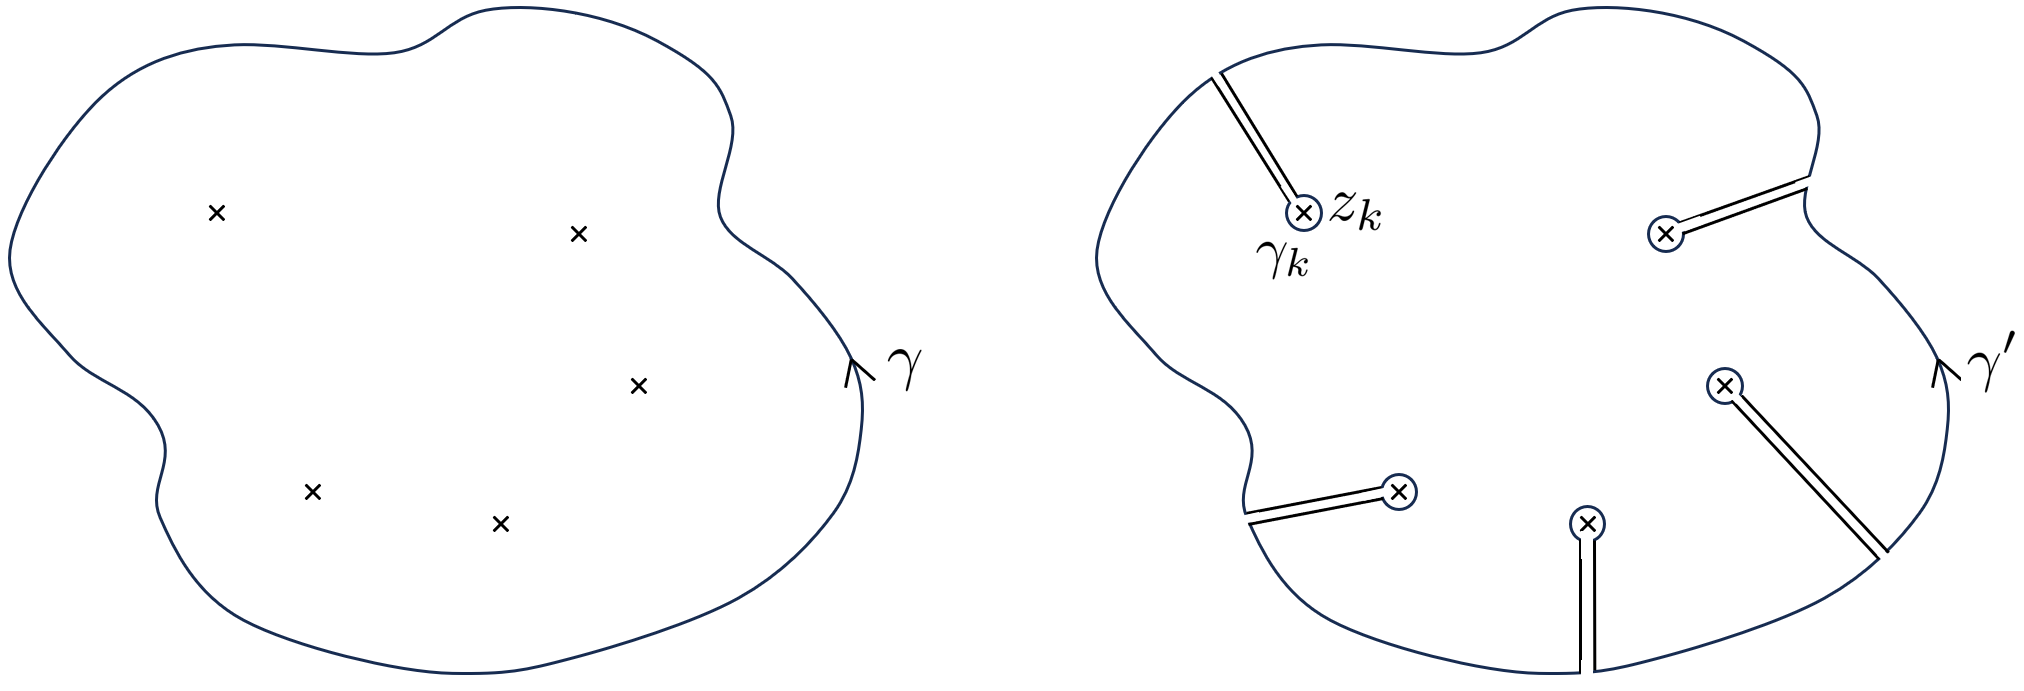
\includegraphics[width=0.8\textwidth]{Residue.png}
	\end{center}

	\begin{proof}
		Consider a new contour \(\gamma'\) by joining \(\gamma\) with contours around each singularity \(\gamma_k\) using `bridges' of width \(\epsilon\) as shown. \(\gamma'\) does not enclose any pole so
		\[\oint_{\gamma'}f(z)\dd{z}=0\,.\]
		At the limit \(\epsilon\to 0\), the `bridges' in the two opposite directions cancel out, so \(\gamma'=\gamma-\sum_k\gamma_k\), and by \cref{reslem}, we have
		\begin{align*}
			\oint_{\gamma'}f(z)\dd{z}&=\oint_\gamma f(z)\dd{z}-\sum_k\oint_{\gamma_k}f(z)\dd{z}\\
			&=\oint_\gamma f(z)\dd{z}-2\pi i\sum_k\res_{z=z_k}f(z)=0\,.
		\end{align*}
		Therefore we have
		\[\oint_\gamma f(z)\dd{z}=2\pi i\sum_k\res_{z=z_k}f(z)\,.\]\qed
	\end{proof}

	\subsection{The Point at Infinity}
	Some functions tend to a definite limit as \(z\to\infty\) irrespective of the direction from which the infinity is approached. e.g. \(f(z)=1/z\) goes to 0 as \(\abs{z}\to\infty\). Therefore, it sometimes makes sense to think of \(\infty\) as a single point, as illustrated by the \textit{stereographic projection} of the complex plane onto \textit{Riemann sphere}.
	\begin{defn}
		\textit{Stereographic projection} may be applied to a unit \(n\)-sphere \(S^n\) in an (\(n+1\))-dimensional Euclidean space \(\mathbb{E}^{n+1}\). If \(Q\) is a point of \(S^n\) and \(E\) is a hyperplane in \(\mathbb{E}^{n+1}\), then the stereographic projection of a point \(P\in S^n-\{Q\}\) is the point \(P'\), intersection of the line \(QP\) with \(E\). The hypersphere of projection is the \textit{Riemann sphere}.
	\end{defn}
	\begin{rem}
		The point \(Q\) in stereographic projection is projected to all points on a circle of infinite radius. We can think of this as a single \textit{point at infinity}.
	\end{rem}
	\begin{defn}
		The \textit{extended complex plane} \(\mathbb{C}_\infty\coloneqq\mathbb{C}\cup\{\infty\}\)
	\end{defn}
	\begin{rem}
		Stereographic projection is a smooth, bijective function from the entire sphere except for the centre of projection to the entire plane. It maps circles on the sphere to circles or lines on the plane, and is conformal (angle-preserving).
	\end{rem}

	The Riemann sphere of the extended complex plane is shown below.

	\begin{figure}[ht!]
		\centering
		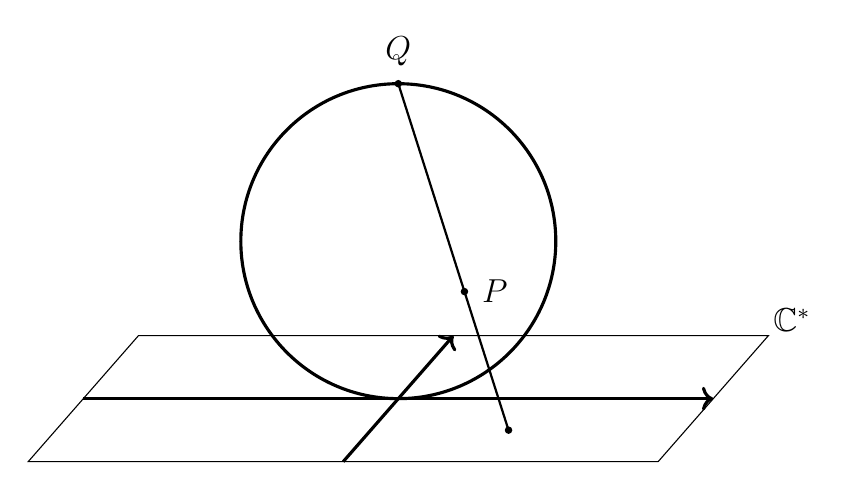
\begin{tikzpicture}
			\draw[line width=0.4mm,->] (-4,0) -- (4,0);
			\draw[line width=0.4mm,->] (-0.7,-0.8) -- (0.7,0.8);
			\draw (3.3,-0.8) -- (4.7,0.8) -- (-3.3,0.8) -- (-4.7,-0.8) -- (3.3,-0.8);
			\draw[line width=0.4mm] (0,2) circle (2);
			\draw[thick] (0,4)--(1.4,-0.4);
			\draw[fill=black] (0,4) circle (0.04) node[above=1mm]{\large\(Q\)};
			\draw[fill=black] (1.4,-0.4) circle (0.04);
			\draw[fill=black] (0.84,1.36) circle (0.04) node[right=1mm]{\large\(P\)};
			\node at (5,1){\large\(\mathbb{C}^*\)};
		\end{tikzpicture}
	\end{figure}

	We can study the behaviour of \(f(z)\) near the point at infinity by defining a new complex variable,
	\[\zeta=\frac{1}{z}\,.\]
	The point at infinity in the \(z\)-plane is the origin in the \(\zeta\)-plane, and vice versa. Setting
	\[g(\zeta)=f\qty(\frac{1}{\zeta})\,,\]
	we can find a Laurent expansion for \(g\) about \(\zeta=0\). If \(g\) has a singularity at \(\zeta=0\) then \(f\) has this singularity at infinity.

	\begin{rem}
		Care must be taken when combining the idea of a point at infinity with the residue theorem because the residue is not strictly a property of \(f\) but of \(f\dd{z}\). For example, if \(\gamma\) is the anticlockwise unit circle in the \(z\)-plane, then
		\[\frac{1}{2\pi i}\oint_\gamma\frac{\dd{z}}{z}=1\,.\]
		But \(\gamma\) is also the clockwise unit circle in the \(\zeta\)-plane. \(\gamma\) may also be viewed as a simple closed contour that encloses the point at infinity in the \(z\)-plane. The integral is therefore equal to minus the sum of the residues outside \(\gamma\). As \(1/z\) has no singularities in the complex plane away from \(z=0\), the residue at \(z=\infty\) must be \(-1\), even though the function \(1/z\) is not singular there.
	\end{rem}
	\subsection{Applications of the Calculus of Residues}
	\subsubsection{Integrals Involving Trigonometric Functions}
	Consider the integral
	\[I=\int_{0}^{2\pi}\frac{\dd{\theta}}{2(a-\cos\theta)}\,,\]
	where \(a>1\) is a real constant. Consider the substitution
	\[z=e^{i\theta}\,.\]
	This gives us \(\dd{z}=iz\dd{\theta}\) and \(\cos\theta=\frac{1}{2}(z+z^{-1})\), while the integral between \(\theta\in[0,2\pi]\) corresponds to the integral over \(z\) around a unit circle \(\gamma\) in the complex plane. Then
	\begin{align*}
		I&=\oint_\gamma\frac{\dd{z}}{2iz\qty(a-\frac{1}{2}(z+z^{-1}))}\\
		&=i\oint_\gamma\frac{\dd{z}}{z^2-2az+1}\\
		&=i\oint_\gamma\frac{\dd{z}}{(z-z_+)(z-z_-)}\,,
	\end{align*}
	where the integrand has simple poles at \(z_\pm=a\pm\sqrt{a^2-1}\).

	Since \(a>1\), it follows that \(z_-\in(0,1)\) and \(z_+>1\). Hence the pole \(z_-\) is inside \(\gamma\) and \(z_+\) is outside it. The residue is
	\[\frac{i}{z_--z_+}=-\frac{i}{2\sqrt{a^2-1}}\,,\]
	so from the residue theorem (\cref{resthm}),
	\[I=\frac{\pi}{\sqrt{a^2-1}}\,.\]

	\subsubsection{Closing a Contour at Infinity}
	Suppose that we wish to calculate the integral
	\[I=\int_{0}^{\infty}\frac{\dd{x}}{x^2+1}\,.\]
	Consider
	\[\oint_\gamma\frac{\dd{z}}{z^2+1}=\oint_{\gamma_0+\gamma_R}\frac{\dd{z}}{(z+i)(z-i)}\,,\]
	where \(\gamma=\gamma_0+\gamma_R\) consists of two parts: first a contour, \(\gamma_0\), from \(-R\) to \(R\) along the real axis, and a second contour, \(\gamma_R\), counterclockwise along a semicircle of radius \(R\) in the upper half plane.

	The integrand has two simple poles, but only the one at \(z=i\) is enclosed by \(\gamma\). Hence, from the residue theorem (\cref{resthm}),
	\[\oint_\gamma\frac{\dd{z}}{z^2+1}=\oint_{\gamma_0+\gamma_R}\frac{\dd{z}}{(z+i)(z-i)}=2\pi i\frac{1}{2i}=\pi\,.\]
	We also have that, using the symmetry of the integrand,
	\[\int_{\gamma_0}\frac{\dd{z}}{z^2+1}\equiv\int_{-R}^{R}\frac{\dd{z}}{z^2+1}=2\int_{0}^{R}\frac{\dd{z}}{z^2+1}\to 2I\text{ as }R\to\infty\,.\]
	Finally, we consider the value of the integral along \(\gamma_R\). On this semicircle, the integrand is \(O(R^{-2})\), while the contour has length \(\pi R\). Hence,
	\[\abs{\int_{\gamma_R}\frac{\dd{z}}{z^2+1}}\le \int_{\gamma_R}\frac{\abs{\dd{z}}}{\min\abs{z^2+1}}\le\frac{\pi R}{R^2-1}\to 0\text{ as }R\to\infty\,.\]
	Combining the above result and taking the limit \(R\to\infty\), we conclude that
	\[I=\frac{\pi}{2}\,.\]
	\begin{rem}
		This method can be easily generalised to contour integrals containing multiple poles.
	\end{rem}

	\subsection{Multi-valued Functions and Branch Cuts}
	Not all complex functions have a single value for each complex point \(z=re^{i\theta}\). For instance, the complex function \(\log z=\ln r+i\theta\) has infinitely many values, or branches, since \(\theta\) can take infinitely many values.

	If a contour \(\gamma\) does not enclose the origin, then we can always choose some range of \(\theta\) so that \(\ln z\) is continuous and single-valued. However, if the contour \(\gamma\) encloses the origin, then \(\ln z\) on the contour can only be multivalued or discontinuous.
	\begin{defn}
		A point that cannot be encircled by a curve where the function is continuous and single-valued is called a \textit{branch point}. The function has a \textit{branch point singularity} at that point.
	\end{defn}
	In order to make a function with a branch point continuous and single-valued on a curve, it is necessary that the curve does not encircle the branch point. To do this, we have to introduce a \textit{branch cut} that no curve is permitted to cross. Having a branch cut, a \textit{branch} of a function is defined such that in the neighbourhood of the branch point, values of \(\theta\) in a \(2\pi\) range are chosen.
	\begin{rem}
		If a curve did cross the cut, the function would be discontinuous and not analytic.
	\end{rem}
	\begin{ex}
		The canonical branch cut for \(\log z\) is along the half real axis from \(-\infty\) to the origin, so that \(\theta\in(-\pi,\pi)\). With this choice of branch cut, the value of \(\log z\) is called the \textit{principal value} of the logarithm, often denoted as \(\mathrm{Log}\,z\).
	\end{ex}
	\begin{rems}
		\begin{itemize}[topsep=0pt]
			\item \(\log z\) has an infinite number of branches.
			\item The complex logarithm is holomorphic everywhere on each branch except on the branch cut.
			\item The function is single-valued and continuous on any curve that does not cross the cut.
			\item Branch cuts need not be straight lines. Any continuous non-intersecting curve from the branch point to infinity can be a branch cut.
		\end{itemize}
	\end{rems}
	
	\begin{cor}
		Multivalued functions have no Laurent expansions about the branch points, since any annulus \(\abs{z-z_0}\in(\alpha,\beta)\) would be crossed by the branch cut so the function would not be analytic in the annulus.
	\end{cor}
	\begin{rem}
		Riemann introduced a different idea where the different branches of a function are regarded as separate copies of the complex plane \(\mathbb{C}\) stacked onto each other and each connected to its neighbours at the respective branch cuts. This is known as the \textit{Riemann surface}.
	\end{rem}

	\begin{ex}
		Consider
		\[f(z)=\sqrt{z^2-1}=\sqrt{z-1}\sqrt{z+1}\,,\]
		a function that has two branch points at \(z=\pm 1\). Setting
		\[z-1=r_1e^{i\theta_1}\text{ and }z+1=r_2e^{i\theta_2}\,,\]
		we see that
		\[f(z)=\sqrt{r_1r_2}e^{\frac{1}{2}i(\theta_1+\theta_2)}\,.\]
		
		If \(z_1\) is enclosed by a small curve \(\gamma_1\), then
		\[\theta_1\to\theta_1+2\pi\,,\;\theta_2\to\theta_2\text{ and }\frac{1}{2}(\theta_1+\theta_2)\to\frac{1}{2}(\theta_1+\theta_2)+\pi\,.\]
		Hence \(f(z)\) changes the sign. The same applies to a small curve \(\gamma_2\) encircling \(z=-1\). However, going around a curve \(\gamma_3\) encircling both branch points has the effect of
		\[\theta_1\to\theta_1+2\pi\,,\;\theta_2\to\theta_2+2\pi\text{ and }\frac{1}{2}(\theta_1+\theta_2)\to\frac{1}{2}(\theta_1+\theta_2)+2\pi\,.\]
		Hence \(f(z)\) does not change the sign.

		Therefore, we can introduce a branch cut that goes from \(z=-1\) to \(z=1\), with the simplest case being a cut on the real axis. Alternatively, we can introduce two separate branch cuts, one from each branch point to infinity.
	\end{ex}
	\begin{rem}
		The two branch cuts to infinity can be seen as a single branch cut that happens to pass through the point at infinity. This is because the cuts can be smoothly deformed. In general, when there is more than one branch point, we may need more than one branch cut.
	\end{rem}
	\subsection{Contour Integration around a Branch Cut}
	Evaluate the integral
	\[I=\int_{0}^{\infty}\frac{x^\alpha}{1+\sqrt{2}x+x^2}\dd{x}\,,\]
	where \(\alpha\in(-1,1)\).
	
	Consider the contour integral
	\[\oint_\gamma\frac{z^\alpha}{1+\sqrt{2}z+z^2}\dd{z}\,.\]
	The integrand has a branch point at \(z=0\), and simple poles at \(z_1=e^{\frac{3}{4}\pi i}\) and \(z_2=e^{\frac{5}{4}\pi i}\).

	We usually find it is appropriate to choose a branch cut along the integration range, i.e. along the positive real axis in this case; we then define the branch by choosing \(0\le\theta<2\pi\), where \(z=re^{i\theta}\).

	It is then necessary to use a `keyhole contour', \(\gamma\), in order to avoid the branch point and the branch cut. We consider the individual contributions from each part of the contour, \(\gamma=\gamma_1+\gamma_R+\gamma_2+\gamma_\epsilon\) in turn.

	\begin{figure}[ht!]
		\centering
		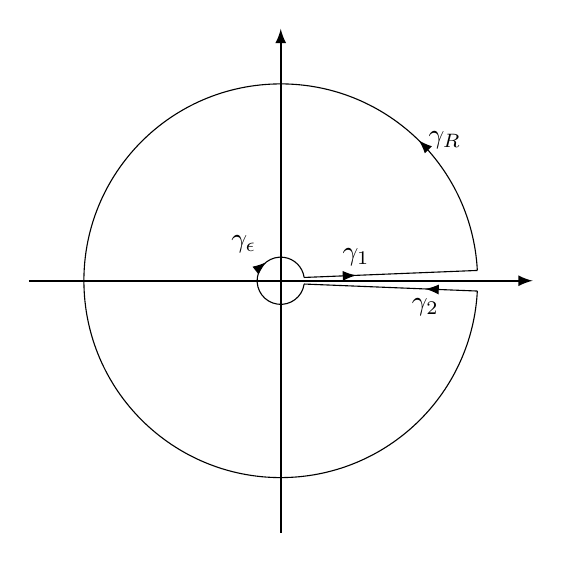
\begin{tikzpicture}[>=latex]
			\draw[thick,->] (-3.2,0)--(3.2,0);
			\draw[thick,->] (0,-3.2)--(0,3.2);

			\draw[
				postaction={decorate},
				decoration={
					markings,
					mark=at position 0.12 with \arrow{Latex[length=1.7mm]},
				}
			]
			(3:2.5) arc (3:357:2.5) node[pos=0.12,right]{\(\gamma_R\)};

			\draw[
				postaction={decorate},
				decoration={
					markings,
					mark=at position 0.65 with \arrow{Latex[length=1.7mm]},
				}
			]
			(352:0.3) arc (352:8:0.3) node[pos=0.65,above left]{\(\gamma_\epsilon\)};

			\draw[
				postaction={decorate},
				decoration={
					markings,
					mark=at position 0.3 with \arrow{Latex[length=1.7mm]},
				}
			]
			(8:0.3)--(3:2.5) node[pos=0.3,above]{\(\gamma_1\)};

			\draw[
				postaction={decorate},
				decoration={
					markings,
					mark=at position 0.3 with \arrow{Latex[length=1.7mm]},
				}
			]
			(357:2.5)--(352:0.3) node[pos=0.3,below]{\(\gamma_2\)};
		\end{tikzpicture}
	\end{figure}

	The contribution from the contour \(\gamma_1\) just above the branch cut is
	\[\int_{\epsilon}^{R}\frac{x^\alpha}{1+\sqrt{2}x+x^2}\dd{x}\to I\]
	as \(\epsilon\to 0\) and \(R\to \infty\).

	Substituting \(z=re^{2\pi i}\), the contribution from the contour \(\gamma_2\) just below the branch cut is
	\[\int_{R}^{\epsilon}\frac{r^\alpha e^{2\pi\alpha i}}{1+\sqrt{2}r+r^2}\dd{r}\to -e^{2\pi\alpha i}I\]
	as \(\epsilon\to 0\) and \(R\to\infty\).

	For \(\gamma_\epsilon\), substitute \(z=\epsilon e^{i\theta}\), we obtain
	\[\int_{\gamma_\epsilon}\frac{z^\alpha}{1+\sqrt{2}z+z^2}\dd{z}=\epsilon^{\alpha+1}\int_{2\pi}^{0}\frac{e^{i(\alpha+1)\theta}}{1+\sqrt{2}\epsilon e^{i\theta}+\epsilon^2 e^{2i\theta}}i\dd{\theta}\to 0\text{ as }\epsilon\to 0\,.\]

	For \(\gamma_R\), substitute \(z=R e^{i\theta}\), we obtain
	\begin{align*}
		\int_{\gamma_R}\frac{z^\alpha}{1+\sqrt{2}z+z^2}\dd{z}&=R^{\alpha+1}\int_{0}^{2\pi}\frac{e^{i(\alpha+1)\theta}}{1+\sqrt{2}R e^{i\theta}+R^2 e^{2i\theta}}i\dd{\theta}\\
		&=R^{\alpha-1}\int_{0}^{2\pi}\frac{e^{i(\alpha+1)\theta}}{R^{-2}+\sqrt{2}R^{-1} e^{i\theta}+e^{2i\theta}}i\dd{\theta}\to 0\text{ as }R\to \infty\,.
	\end{align*}

	Therefore, as \(\epsilon\to 0\) and \(R\to\infty\),
	\[\oint_\gamma\frac{z^\alpha}{1+\sqrt{2}z+z^2}=\oint_{\gamma_1+\gamma_R+\gamma_2+\gamma_\epsilon}\frac{z^\alpha}{(z-z_1)(z-z_2)}\dd{z}\to (1-e^{2\pi\alpha i})I\,.\]
	Because both poles are inside \(\gamma\), the residue theorem gives
	\[\res_{z=z_1}\frac{z^\alpha}{(z-z_1)(z-z_2)}=\frac{z_1^\alpha}{z_1-z_2}=\frac{e^{\frac{3}{4}\pi\alpha i}}{e^{\frac{3}{4}\pi\alpha i}-e^{\frac{5}{4}\pi\alpha i}}\,,\]
	\[\res_{z=z_2}\frac{z^\alpha}{(z-z_1)(z-z_2)}=\frac{z_2^\alpha}{z_2-z_1}=\frac{e^{\frac{5}{4}\pi\alpha i}}{e^{\frac{5}{4}\pi\alpha i}-e^{\frac{3}{4}\pi\alpha i}}\,,\]
	\[(1-e^{2\pi\alpha i})I=2\pi i\qty(\frac{e^{\frac{3}{4}\pi\alpha i}}{i\sqrt{2}}-\frac{e^{\frac{5}{4}\pi\alpha i}}{i\sqrt{2}})\,,\]
	and so
	\[I=\sqrt{2}\pi\frac{\sin(\frac{\alpha \pi}{4})}{\sin(\alpha\pi)}\,.\]
	
	\newpage

	\section{Transform Methods}\label{Chap:Transform_methods}
	\subsection{Jordan's Lemma}
	Consider
	\[\lim_{R\to\infty}\int_{\gamma}g(z)e^{i\lambda z}\dd{z}\,,\]
	where
	\begin{enumerate}[topsep=0pt]
		\item \(\lambda\) is a real positive constant;
		\item \(g(z)\) is holomorphic in the upper half-plane except possibly at a finite number of poles;
		\item the contour \(\gamma\) is a semicircle of radius \(R\) in the upper half-plane: \(\gamma:[0,\pi]\to\mathbb{C}\), \(\theta\mapsto Re^{i\theta}\).
	\end{enumerate}
	\begin{lem}\label[lem]{upperjordan}
		The upper bound for the contour integral is given by
		\[\abs{\int_{\gamma}g(z)e^{i\lambda z}\dd{z}}\le\frac{\pi}{\lambda}M_R\,,\]
		where
		\[M_R=\sup_{\theta\in[0,\pi]}\abs{g(Re^{i\theta})}\,,\]
		with equality when \(g\) vanishes everywhere.
	\end{lem}
	\begin{proof}
		Since on \(\gamma\),
		\[\abs{e^{i\lambda z}}=\abs{e^{-\lambda R\sin\theta}}\,,\]
		we have
		\begin{align*}
			\abs{\int_{\gamma}g(z)e^{i\lambda z}\dd{z}}&\le\int_{\gamma}\abs{e^{i\lambda z}g(z)}\abs{\dd{z}}\\
			&=M_RR\int_{0}^{\pi}e^{-\lambda R\sin\theta}\dd{\theta}\\
			&=2M_RR\int_{0}^{\frac{\pi}{2}}e^{-\lambda R\sin\theta}\dd{\theta}\,.
		\end{align*}
		Using the inequality that for \(\theta\in[0,\pi/2]\),
		\[1\ge\frac{\sin\theta}{\theta}\ge\frac{2}{\pi}\,,\]
		\begin{align*}
			\int_{\gamma}g(z)e^{i\lambda z}\dd{z}&\le 2M_RR\int_{0}^{\frac{\pi}{2}}e^{-\lambda R\frac{2\theta}{\pi}}\dd{\theta}\\
			&=\frac{\pi M_R}{\lambda}(1-e^{-\lambda R})\\
			&\le\frac{\pi M_R}{\lambda}\,,
		\end{align*}
		with equality when \(g\) is identically \(0\).\qed
	\end{proof}
	\begin{rem}
		An analogous statement for a semicircular clockwise contour in the lower half-plane holds when \(\lambda<0\).
	\end{rem}
	\begin{rem}
		For the case \(\lambda=0\), this reduces to the ML estimation lemma (\cref{estlem}).
	\end{rem}
	\begin{lem}[Jordan's Lemma]\label[lem]{jdlem}
		If \(g(z)\to 0\) uniformly on \(\gamma\) as \(R\to\infty\), i.e. if
		\[\lim_{R\to\infty}M_R=0\,,\]
		then
		\[\lim_{R\to\infty}\int_{\gamma}g(z)e^{i\lambda z}\dd{z}=0\,.\]
	\end{lem}
	\begin{proof}
		It follows trivially from \cref{upperjordan}.\qed
	\end{proof}
	\subsubsection{Example of Jordan's Lemma}
	Consider
	\[I=\int_{-\infty}^{\infty}\frac{\sin x}{x}\dd{x}\,.\]

	Note that the singularity at the origin is removable. Since \(\sin z=\frac{1}{2i}(e^{iz}-e^{-iz})\), we can apply Jordan's lemma by splitting up the integral.
	\begin{align*}
		I&=\frac{1}{2i}\qty(\int_{-\infty}^{\infty}\frac{e^{iz}}{z}\dd{z}-\int_{-\infty}^{\infty}\frac{e^{-iz}}{z}\dd{z})\\
		&=\Im\qty(\int_{-\infty}^{\infty}\frac{e^{iz}}{z})\,.
	\end{align*}
	But now the contour passes through a pole, so instead consider the limit
	\begin{align*}
		I=\Im\qty[\lim_{\epsilon\to 0}\lim_{R\to\infty}\qty(\int_{-R}^{\epsilon}\frac{e^{iz}}{z}\dd{z}+\int_{\epsilon}^{R}\frac{e^{iz}}{z}\dd{z})]\,.
	\end{align*}
	Define the contour \(\Gamma=\gamma_R+\gamma_-+\gamma_\epsilon+\gamma_+\), where
	\[\begin{cases}
		\gamma_R:\theta\mapsto Re^{i\theta} &,\;\theta\in[0,\pi]\\
		\gamma_-:t\mapsto t &,\;t\in[-R,-\epsilon]\\
		\gamma_\epsilon:\theta\mapsto\epsilon e^{i(\pi-\theta)} &,\;\theta\in[0,\pi]\\
		\gamma_+:t\mapsto t &,\;t\in[\epsilon,R]\,.
	\end{cases}\]
	Then since \(\Gamma\) does not enclose any pole, from Cauchy's theorem (\cref{cauthm}),
	\begin{align*}
		\oint_\Gamma\frac{e^{iz}}{z}\dd{z}&=\int_{\gamma_R}\frac{e^{iz}}{z}\dd{z}+\int_{\gamma_-}\frac{e^{iz}}{z}\dd{z}+\int_{\gamma_\epsilon}\frac{e^{iz}}{z}\dd{z}+\int_{\gamma_+}\frac{e^{iz}}{z}\dd{z}\\
		&=0\,.
	\end{align*}
	On \(\gamma_\epsilon\), \(z=\epsilon e^{i(\pi-\theta)}\), so
	\begin{align*}
		\int_{\gamma_\epsilon}\frac{e^{iz}}{z}\dd{z}&=\int_{\pi}^{0}\frac{\exp(i\epsilon e^{i\theta})}{\epsilon e^{i\theta}}i\epsilon e^{i\theta}\dd{\theta}\\
		&=-i\int_{0}^{\pi}\sum_{r=0}^{\infty}\frac{i^r\epsilon^r e^{ir\theta}}{r !}\dd{\theta}\\
		&=-i\int_{0}^{\pi}1+O(\epsilon)\dd\theta\,.
	\end{align*}
	Thence,
	\[\lim_{\epsilon\to 0}\int_{\gamma_\epsilon}\frac{e^{iz}}{z}\dd{z}=-i\pi\,.\]
	Further, from Jordan's lemma, we know that
	\[\lim_{R\to\infty}\int_{\gamma_R}\frac{e^{iz}}{z}\dd{z}=0\,.\]
	Hence, taking the double limit \(\epsilon\to 0\) and \(R\to\infty\), we have
	\begin{align*}
		I&=\Im\lim_{\epsilon\to 0}\lim_{R\to\infty}\qty(-\int_{\gamma_R}\frac{e^{iz}}{z}\dd{z}-\int_{\gamma_\epsilon}\frac{e^{iz}}{z}\dd{z})\\
		&=\Im(i\pi)=\pi\,.
	\end{align*}
	\begin{rem}
		Similar methods can be used to evaluate
		\[\int_{-\infty}^{\infty}\frac{\sin^{2}x}{x^2}\dd{x}\,.\]
	\end{rem}

	\subsection{Fourier Transform Methods}
	Here, we will state a more precise version of the Fourier transform that allows us to incorporate techniques of contour integrations.
	\begin{defn}
		The \textit{Cauchy principal value} of the integral of an integrable function \(f\) in the range \((-\infty,\infty)\) is given by
		\[\mathrm{PV}\int_{-\infty}^{\infty}f(x)\dd{x}\equiv\fint_{-\infty}^{\infty}f(x)\dd{x}\coloneqq\lim_{R\to\infty}\int_{-R}^{R}f(x)\dd{x}\,.\]
	\end{defn}
	\begin{rem}
		Some functions do not have integral from \(-\infty\) to \(\infty\) in the normal sense, but have Cauchy principal value. For example,
		\[\fint_{-\infty}^{\infty}\frac{x}{1+x^2}\dd{x}=0\]
		but
		\[\int_{-\infty}^{\infty}\frac{x}{1+x^2}\dd{x}\]
		does not converge.
	\end{rem}
	\begin{defn}\label[defn]{ft}
		Let \(f:\mathbb{R}\to\mathbb{C}\) be absolutely integrable, i.e. \(\int_{-\infty}^{\infty}\abs{f(x)}\dd{x}\) exists, has bounded variation and a finite number of discontinuities. The \textit{Fourier transform} of a function \(f(x)\) is
		\[\tilde{f}(k)\equiv\mathcal{F}[f(x)]\coloneqq\fint_{-\infty}^{\infty}f(x)e^{-ikx}\dd{x}\,.\]
	\end{defn}
	\begin{rem}
		Sometimes we can take the Fourier transform of functions that do not satisfy the requirement of absolute integrability, like \(f(x) = 1\). These can be handled using distributions.
		\[\tilde{f}(k)=2\pi\delta(k)\,.\]
	\end{rem}
	\begin{thm}[Fourier inversion theorem]\label{ift}
		The inverse Fourier transform acting on \(\tilde{f}(k)\),
		\[\frac{1}{2}(f(x^+)+f(x^-))=\frac{1}{2\pi}\fint_{-\infty}^{\infty}\tilde{f}(k)e^{ikx}\dd{k}\,,\]
		returns \(f(x)\) when it is continuous while giving the average value of the left and right hand side limits at a discontinuity.
	\end{thm}
	\subsubsection{Fourier Transform using Contour Integration}
	\begin{ex}
		Consider the inverse Fourier transform of
		\[f(x)=\frac{1}{a+ix}\,,\]
		where \(a>0\) is a constant. Let \(\gamma_0\) be the contour from \(-R\) to \(R\) in the real axis, \(\gamma_R\) be the semicircle of radius \(R\) in the upper half-plane, \(\gamma_R'\) be the semicircle in the lower half-plane. We let \(\gamma=\gamma_0+\gamma_R\) and \(\gamma'=\gamma_0+\gamma_R'\).

		\begin{figure}[ht!]
			\centering
			\begin{tikzpicture}[>=latex,scale=1.1]
				\draw[->] (-3,0)--(3,0);
				\draw[->] (0,-3)--(0,3);

				\draw[
					thick,
					postaction={decorate},
					decoration={
						markings,
						mark=at position 0.3 with \arrow{Latex[length=1.7mm]},
					}
				]
				(2,0) arc (0:180:2)node[pos=0.3,right=1mm]{\(\gamma_R\)};

				\draw[
					thick,
					postaction={decorate},
					decoration={
						markings,
						mark=at position 0.7 with \arrow{Latex[length=1.7mm]},
					}
				]
				(-2,0) -- (2,0)node[pos=0.7,above=1mm]{\(\gamma_0\)};

				\draw[
					thick, dashed,
					postaction={decorate},
					decoration={
						markings,
						mark=at position 0.3 with \arrowreversed{Latex[length=1.7mm]},
					}
				]
				(-2,0) arc (180:360:2)node[pos=0.3,left=1mm]{\(\gamma_R'\)};
				\node at (0,1){\(\bm{\times}\)};
			\end{tikzpicture}
		\end{figure}

		We can see that \(f(x)\) has only one single pole at \(x=ia\), so we get
		\[\oint_\gamma f(x)e^{-ikx}\dd{x}=2\pi i\res_{x=ia}\frac{e^{-ikx}}{i(x-ia)}=2\pi e^{ka}\,.\]
		While we have
		\[\oint_{\gamma'}f(x)e^{-ikx}\dd{x}=0\,.\]

		Now, if \(k<0\), applying Jordan's lemma with \(\lambda=-k\) to \(\gamma_R\) gives that
		\[\int_{\gamma_R}f(x)e^{-ikx}\dd{x}\to 0\text{ as }R\to\infty\,.\]
		Hence,
		\begin{align*}
			\tilde{f}(k)&=\fint_{-\infty}^{\infty}f(x)e^{-ikx}\dd{x}\\
			&=\lim_{R\to\infty}\int_{\gamma_0}f(x)e^{-ikx}\dd{x}\\
			&=\lim_{R\to\infty}\qty(\int_{\gamma}f(x)e^{-ikx}\dd{x}-\int_{\gamma_R}f(x)e^{-ikx}\dd{x})\\
			&=2\pi e^{ka}\,.
		\end{align*}
		
		For \(k>0\), we close the contour in the lower half plane. Since there is no singularity, we get
		\[\int_{-\infty}^{\infty}f(x)e^{-ikx}\dd{x}=0\,.\]

		Therefore,
		\[\tilde{f}(k)=\begin{cases}
			0 & k>0\\
			2\pi e^{ak} & k<0\,.
		\end{cases}\]
	\end{ex}

	\subsubsection{Damped Harmonic Oscillator}
	Consider the equation for the amplitude \(x(t)\) of a driven damped harmonic oscillator,
	\begin{equation}\tag{\(\dagger\)}
		\ddot{x}(t)+2\gamma\dot{x}(t)+\omega_0^2 x(t)=f(t)\,,
	\end{equation}
	where \(f(t)\) is the forcing function, \(\omega_0>0\) is real, and \(\gamma>0\) is real and represents the effects of damping.

	Assume that \(x(t)\to 0\) as \(\abs{t}\to\infty\) so that we can define Fourier transform, and its inverse, of \(x(t)\) as
	\[\tilde{x}(\omega)=\int_{-\infty}^{\infty}x(t)e^{-i\omega t}\dd{t}\]
	\[x(t)=\frac{1}{2\pi}\int_{-\infty}^{\infty}\tilde{x}(\omega)e^{i\omega t}\dd{\omega}\,,\]
	where we use \(\omega\) as the Fourier variable when the function depends on \(t\) as is conventional.

	By \cref{ftdif}, we have
	\[\mathcal{F}[\dot{x}(t)]=i\omega\tilde{x}(\omega)\]
	\[\mathcal{F}[\ddot{x}(t)]=-\omega^2\tilde{x}(\omega)\,.\]
	Take Fourier transform on both sides of (\(\dagger\)), we have
	\[(-\omega^2+2i\gamma\omega+\omega_0^2)\tilde{x}(\omega)=\tilde{f}(\omega)\,.\]
	It follows that
	\[\tilde{x}(\omega)=\tilde{f}(\omega)\tilde{g}(\omega)\,,\]
	where
	\begin{align*}
		\tilde{g}(\omega)&=\frac{-1}{\omega^2-2i\gamma\omega-\omega_0^2}\\
		&=\frac{-1}{(\omega-\omega_+)(\omega-\omega_-)}\qquad\text{and }\omega_\pm=i\gamma\pm\sqrt{\omega_0^2-\gamma^2}\,.
	\end{align*}
	We can find \(x(t)\) by taking the inverse Fourier transform
	\[x(t)=\frac{1}{2\pi}\int_{-\infty}^{\infty}\tilde{f}(\omega)\tilde{g}(\omega)e^{i\omega t}\dd{\omega}\,.\]

	Recall that the convolution theorem (\cref{conthm}) states
	\[h(t)=\int_{-\infty}^{\infty}f(s)g(t-s)\dd{s}\iff \tilde{h}(\omega)=\tilde{f}(\omega)\tilde{g}(\omega)\,.\]
	Hence, we deduce that
	\[x(t)=\int_{-\infty}^{\infty}f(s)g(t-s)\dd{s}\,,\]
	where, with \(\tau=t-s\),
	\[g(\tau)=\mathcal{F}^{-1}[\tilde{g}(\omega)]=-\frac{1}{2\pi}\int_{-\infty}^{\infty}\frac{e^{i\omega\tau}}{(\omega-\omega_+)(\omega-\omega_-)}\dd{\omega}\,.\]

	\begin{rem}
		This is equivalent to a solution using the Green's function \(G(t,s)=g(t-s)\) of
		\[L=\dv[2]{t}+2\gamma\dv{t}+\omega_0^2\,.\]
	\end{rem}

	To complete the solution to the problem, we now have to determine \(g(\tau)\) by integrating over \(\omega\). We will do this by employing a contour integral in the complex \(\omega\) plane.

	If \(\tau<0\), we choose a contour \(\gamma\) that goes along the real axis and is closed with a semicircle in the lower half-plane (\(\gamma_\infty\)). If \(\tau>0\) we instead close the contour with a semicircle in the upper half plane. Since, by our assumption, \(\tilde{g}(\omega)\to 0\) as \(\abs{\omega}\to\infty\), Jordan's lemma (\cref{jdlem}) implies that in both cases the integral over the semicircle will vanish. It then follows that
	\begin{align*}
		g(\tau)&=\frac{1}{2\pi}\int_{-\infty}^{\infty}\tilde{g}(\omega)e^{i\omega\tau}\dd{\omega}\\
		&=\frac{1}{2\pi}\qty(\int_{-\infty}^{\infty}\tilde{g}(\omega)e^{i\omega\tau}\dd{\omega}+\int_{\gamma_\infty}\tilde{g}(\omega)e^{i\omega\tau}\dd{\omega})\\
		&=\frac{1}{2\pi}\oint_\gamma\tilde{g}(\omega)e^{i\omega\tau}\dd{\omega}\,.
	\end{align*}

	As long as \(\omega_0\) is real, so that \(\omega_0^2>0\), poles of \(\tilde{g}(\omega)\) at \(\omega=\omega_\pm\) are both in the upper half plane. Therefore, from the residue theorem,
	\[g(\tau)=0\quad\text{when}\quad\tau<0\,.\]
	In other words, \(g(t-s)\) is zero if \(t<s\). Suppose that the forcing term is not switched on until \(t=0\), i.e. suppose that \(f(t)=0\) for \(t<0\), it follows that
	\[x(t)=\int_{0}^{\infty}f(s)g(t-s)\dd{s}=0\quad\text{for}\quad t<0\,.\]
	\begin{rem}
		This means that there is no response until the forcing term is switched on. This is a \textit{causal behaviour}, i.e. effect follows cause and not the other way around. The Green's function, \(G(t,s)=g(t-s)\) is said to be a \textit{causal Green's function.}
	\end{rem}

	For \(\tau>0\), there are two simple poles within \(\gamma\). As we assume that \(\gamma\ne\omega_0\), the residue at \(\omega=\omega_\pm\) are given by
	\[\res_{\omega=\omega_\pm}\qty(\frac{1}{2\pi}\tilde{g}e^{i\omega\tau})=\frac{-e^{i\omega_\pm\tau}}{2\pi(\omega_\pm-\omega_\mp)}=\mp\frac{e^{-\gamma\tau}e^{\pm i\tau\sqrt{\omega_0^2-\gamma^2}}}{4\pi\sqrt{\omega_0^2-\gamma^2}}\,.\]

	\begin{itemize}
		\item \textit{Underdamped Oscillator.} For \(\gamma<\omega_0\), the oscillator is said to be \textit{underdamped}. We can deduce that
		\[g(\tau)=\frac{e^{-\gamma\tau}}{\sqrt{\omega_0^2-\gamma^2}}\sin(\tau\sqrt{\omega_0^2-\gamma^2})\quad\text{for }\tau>0\,.\]
		\begin{rem}
			Suppose that there is a unit impulse at \(t=0\), i.e. \(f(t)=\delta(t)\). It follows that \(x(t)=g(t)\), and hence the response to an impulsive force is oscillatory with an amplitude that dies away exponentially over a time of order \(1/\gamma\).

			For \(\gamma\ll \omega_0\), the main effect of the damping term is to cause the oscillation to slowly reduce in amplitude rather than change phase.
		\end{rem}

		\item \textit{Overdamped Oscillator.} For \(\gamma>\omega_0\), the oscillator is said to be \textit{overdamped}. We can deduce that
		\[g(\tau)=\frac{e^{-\gamma\tau}}{\sqrt{\gamma^2-\omega_0^2}}\sinh(\tau\sqrt{\gamma^2-\omega_0^2})\quad\text{for }\tau>0\,.\]

		\item \textit{Critically Damped Oscillator.} When \(\gamma=\omega_0\), the oscillator is critically damped. For \(\tau>0\), there is a double pole at \(\omega=i\gamma\) inside the contour \(\gamma\). From \cref{resfor}, we have
		\begin{align*}
			\res_{\omega=i\gamma}\qty(\frac{1}{2\pi}\tilde{g}e^{i\omega\tau})&=\res_{\omega=i\gamma}\qty(-\frac{e^{i\omega\tau}}{2\pi(\omega-i\gamma)^2})\\
			&=\lim_{\omega\to i\gamma}\qty(\dv{\omega}\qty(-\frac{e^{i\omega\tau}}{2\pi}))\\
			&=-\frac{i\tau e^{-\gamma\tau}}{2\pi}\,.
		\end{align*}
		Hence, the residue theorem yields
		\[g(\tau)=\tau e^{-\gamma\tau}\quad\text{for }\tau>0\,.\]
	\end{itemize}
	\subsubsection{Gaussian Integration Lemma}
	\begin{lem}[Gaussian integration lemma]\label[lem]{gaussintlem}
		For any constant \(c\in\mathbb{C}\),
		\[\int_{-\infty}^{\infty}e^{-(u+c)^2}\dd{u}=\sqrt{\pi}\,.\]
	\end{lem}
	\begin{proof}
		Let \(c=a+bi\). Extend the integral to the complex plane, and define a new complex variable \(z=u+c\). Then
		\[I=\int_{-\infty}^{\infty}e^{-(u+c)^2}\dd{u}=\int_{\gamma_i}e^{-z^2}\dd{z}\,,\]
		where the contour \(\gamma_i\) is the horizontal line in the complex \(z\) plane with \(\Im z=\Im c=b\).

		The integrand \(e^{-z^2}\) is analytic everywhere and so the integral of \(e^{-z^2}\) around any closed contour is zero.

		Consider the rectangular counterclockwise contour with vertices at \(\pm R\) and \(\pm R+ib\), \(R\in\mathbb{R}\).

		Apply Cauchy's theorem to this contour to obtain
		\begin{align*}
			0&=\lim_{R\to\infty}\oint_{\gamma_R}e^{-z^2}\dd{z}\\
			&=\lim_{R\to\infty}\qty[\int_{-R}^{R}e^{-z^2}\dd{z}+\int_{0}^{b}e^{-(R+iy)^2}i\dd{y}+\int_{R+ib}^{-R+ib}e^{-z^2}\dd{z}+\int_{b}^{0}e^{-(-R+iy)^2}i\dd{y}]\\
			&=\sqrt{\pi}-I+\lim_{R\to\infty}2e^{-R^2}\int_{0}^{b}e^{y^2}\sin(2Ry)\dd{y}\,.
		\end{align*}
		In the limit \(R\to\infty\) the final term tends to zero, and so we deduce that, for any \(c\in\mathbb{C}\),
		\[I=\int_{-\infty}^{\infty}e^{-(u+c)^2}\dd{u}=\sqrt{\pi}\,.\]\qed
	\end{proof}
	\subsubsection{Solutions to Partial Differential Equations}
	Consider the initial-boundary value problem of the heat distribution on an infinite bar:
	\[\left\{\begin{aligned}
		\, & \pdv{\theta}{t}=\lambda\pdv[2]{\theta}{x} && (x,t)\in\mathbb{R}\cross(0,\infty)\\
		\, & \theta(x,0)=f(x) && x\in\mathbb{R}\\
		\, & \pdv{\theta}{x}\to 0 && \text{as }x\to\pm\infty,t\in(0,\infty)\,.
	\end{aligned}\right.\]

	Take the Fourier transform of the equation, we have
	\[\pdv{\tilde{\theta}}{t}=-\lambda k^2\tilde{\theta}\,.\]
	The solution of this equation is
	\[\tilde{\theta}(k,t)=\tilde{\theta}_0(k)e^{-\lambda k^2 t}\,.\]
	Applying the initial condition, we have
	\(\tilde{\theta}_0(k)=\tilde{f}(k)\). Rewrite the expression of the transformed solution as
	\[\tilde{\theta}(k,t)=\tilde{f}(k)\tilde{G}(k,t)\,,\]
	where
	\[\tilde{G}(k,t)=e^{-\lambda k^2t}\,.\]
	By the convolution theorem, the solution is
	\[\theta(x,t)=\theta(x)*G(x,t)=\int_{-\infty}^{\infty}\theta_0(y)G(x-y,t)\dd{y}\,,\]
	where using the substitution \(u=\sqrt{\lambda t}k\), \(G(x,t)\) can be evaluated as
	\begin{align*}
		G(x,t)&=\frac{1}{2\pi}\int_{-\infty}^{\infty}e^{ikx-\lambda kt^2}\dd{k}\\
		&=\frac{e^{-\frac{x^2}{4\lambda t}}}{2\pi\sqrt{\lambda t}}\int_{-\infty}^{\infty}\exp(-\qty(u-\frac{ix}{2\sqrt{\lambda t}})^2)\dd{u}\\
		&=\frac{e^{-\frac{x^2}{4\lambda t}}}{\sqrt{4\pi\lambda t}}
	\end{align*}
	by the Gaussian integration lemma. Hence,
	\[\theta(x,t)=\frac{1}{\sqrt{4\pi\lambda t}}\int_{-\infty}^{\infty}f(y)\exp(-\frac{(x-y)^2}{4\lambda t})\dd{y}\,.\]

	Let us consider the specific case \(f(x)=H(x)\), the Heaviside step function.

	Recall the error function:
	\begin{defn}
		The \textit{error function} is defined as
		\[\mathrm{erf}(x)\coloneqq\frac{2}{\sqrt{\pi}}\int_{0}^{x}e^{-t^2}\dd{t}\]
		such that \(\mathrm{erf}(-\infty)=-1\) and \(\mathrm{erf}(\infty)=1\).
	\end{defn}

	Then, using the substitution \(v=\frac{y-x}{\sqrt{4\lambda t}}\),
	\begin{align*}
		\theta(x,t)&=\frac{1}{\sqrt{4\pi\lambda t}}\int_{0}^{\infty}\exp(-\frac{(x-y)^2}{4\lambda t})\dd{y}\\
		&=\frac{1}{\sqrt{\pi}}\int_{-\frac{x}{\sqrt{4\lambda t}}}^{\infty}e^{-v^2}\dd{v}\\
		&=\frac{1}{\sqrt{\pi}}\qty[\int_{0}^{\infty}e^{-v^2}\dd{v}+\int_{0}^{\frac{x}{\sqrt{4\lambda t}}}e^{-v^2}\dd{v}]\\
		&=\frac{1}{2}\qty[1+\mathrm{erf}\qty(\frac{x}{\sqrt{4\lambda t}})]\,.
	\end{align*}
	\subsection{Laplace Transforms (Non-examinable)}
	The main shortcoming of Fourier transforms is the restriction to absolutely integrable functions. Many systems encountered in the real world involve growing functions, such as \(e^t\), which we cannot manage with Fourier transforms, not even by resorting to distributional theory.
	
	The Laplace transform provides a handle to treat such functions in a manner analogous to the Fourier domain. Furthermore, we will see that Laplace transforms have a natural way of incorporating boundary conditions, which makes them very suitable for solving ordinary differential equations.

	\subsubsection{Laplace Transform and Analytic Continuation}
	\begin{defn}
		Let \(f(t)\) be a function defined for all \(t\ge 0\). The \textit{Laplace transform} of \(f(t)\) is given by
		\[F(s)=\lt{f(t)}(s)\coloneqq\int_{0}^{\infty}f(t)e^{-st}\dd{t}\,,\]
		\(s\in\mathbb{C}\) provided that the integral exists.
	\end{defn}
	\begin{rem}
		A sufficient condition for the existence of a Laplace transform is that \(f(t)\) grows no more than exponential.
	\end{rem}

	Let us consider a very important example. By direct integration, we can find
	\[\lt{1}(s)=\int_{0}^{\infty}e^{-st}\dd{t}=\frac{1}{s}\,,\]
	which may look completely trivial. However, notice that this integral only converges for \(\Re(s)>0\). Despite this, we may still extend the domain of the Laplace transform function \(F(s)\) to the entire range where it is defined analytically. This process is the analytic continuation. In this case, we extended the domain of the Laplace transform from \(U'=\{z\in\mathbb{C}\mid \Re(z)>0\}\) to \(U=\mathbb{C}\setminus\{0\}\), where the uniqueness of the extended function is guaranteed by the analyticity of the transformed function.

	Here are some further examples.
	\begin{itemize}[topsep=0pt]
		\item We can integrate by parts to find
		\[\lt{t}(s)=\int_{0}^{\infty}te^{-st}\dd{t}=\qty[-\frac{t}{s}e^{-ts}]_{t=0}^{\infty}+\int_{0}^{\infty}\frac{1}{s}e^{-st}\dd{t}=\frac{1}{s^2}\,.\]
		\item For a constant \(\lambda\), we can directly integrate
		\[\lt{e^{\lambda t}}(s)=\int_{0}^{\infty}e^{(\lambda-s)t}\dd{t}=\frac{1}{s-\lambda}\,.\]
		Again, this integral is only defined if \(\Re(s)>\Re(\lambda)\), but we can analytically continue the function for all \(s\in\mathbb{C}\) except \(s=\lambda\).
		\item Using the previous result, we find that
		\[\lt{\sin t}=\lt{\frac{1}{2i}(e^{it}-e^{-it})}(s)=\frac{1}{2i}\qty(\frac{1}{s-i}-\frac{1}{s+i})=\frac{1}{s^2+1}\,.\]
	\end{itemize}
	\subsubsection{Properties of the Laplace Transform}
	\begin{prop}\label[prop]{ltprop}
		The Laplace transform has the following properties.
		\begin{enumerate}[topsep=0pt]
			\item \textit{Linearity.} For constants \(\alpha,\beta\in\mathbb{C}\),
			\[\lt{\alpha f+\beta g}=\alpha\lt{f}+\beta\lt{g}\,.\]
			\item \textit{Translation.} For real constant \(t_0\in\mathbb{R}\),
			\[\lt{f(t-t_0)H(t-t_0)}(s)=e^{-st_0}F(s)\,.\]
			\item \textit{Scaling.} For constant \(\lambda>0\),
			\[\lt{f(\lambda t)}(s)=\frac{1}{\lambda}F\qty(\frac{s}{\lambda})\,.\]
			\item \textit{Shifting.} For a constant \(s_0\in\mathbb{C}\),
			\[\lt{e^{s_o t}f(t)}(s)=F(s-s_0)\,.\]
			\item \textit{Transform of a derivative.}
			\[\lt{f'(t)}(s)=sF(s)-f(0)\,.\]
			By repeatedly applying this formula, we find
			\[\lt{f''(t)}(s)=s\lt{f'(t)}(s)-f'(0)=s^2F(s)-sf(0)-f'(0)\]
			and so forth.
			\item \textit{Derivative of a transform.}
			\[F'(s)=\lt{-tf(t)}(s)\,.\]
			More generally,
			\[F^{(n)}(s)=\lt{(-t)^n f(t)}(s)\,.\]
			\item \textit{Asymptotic limit.}
			\[\lim_{s\to\infty}s F(s)=f(0)\,,\]
			\[\lim_{s\to 0}sF(s)=f(\infty)\,,\]
			provided that the limit \(\lim_{t\to\infty}f(t)\) exists.
		\end{enumerate}
	\end{prop}
	\begin{proofskip}
		\begin{enumerate}[topsep=0pt]
			\item Follows from the linearity of integrals.
			\item Setting \(\tilde{t}=t-t_0\), we have
			\begin{align*}
				\int_{0}^{\infty}f(t-t_0)e^{-st}\dd{t}&=\int_{-t_0}^{\infty}f(\tilde{t})e^{-s(\tilde{t}+t_0)}\dd{\tilde{t}}\\
				&=e^{-st_0}\int_{-t_0}^{\infty}f(\tilde{t})e^{-s\tilde{t}}\dd{\tilde{t}}\,.
			\end{align*}
			So
			\begin{align*}
				\int_{0}^{\infty}f(t-t_0)H(t-t_0)e^{-st}\dd{t}&=e^{-st_0}\int_{-t_0}^{\infty}f(\tilde{t})H(\tilde{t})e^{-s\tilde{t}}\dd{\tilde{t}}\\
				&=e^{-st_0}\int_{0}^{\infty}f(\tilde{t})e^{-s\tilde{t}}\dd{\tilde{t}}=e^{-st_0}F(s)\,.
			\end{align*}
			\item Define \(\tilde{t}=\lambda t\), we find
			\[\int_{0}^{\infty}f(\lambda t)e^{-st}\dd{t}=\int_{0}^{\infty}f(\tilde{t})e^{-\frac{s}{\lambda}\tilde{t}}\frac{1}{\lambda}\dd{\tilde{t}}=\frac{1}{\lambda}F\qty(\frac{s}{\lambda})\,.\]
			\item 
			\[\int_{0}^{\infty}e^{s_0 t}f(t)e^{-st}\dd{t}=F(s-s_0)\,.\]
			\item
			\[\int_{0}^{\infty}f'(t)e^{-st}\dd{t}=[f(t)e^{-st}]_{t=0}^\infty-\int_{0}^{\infty}-sf(t)e^{-st}\dd{t}=sF(s)-f(0)\,.\]
			Once again, we encounter the subtlety of analytic continuation. The proof breaks down if the integral \(\int_{0}^{\infty} f(t)e^{-st}\dd{t}\) does not exist. The relation still holds for analytically continued Laplace transforms, though.
			\item Differentiating the definition of the Laplace transform gives
			\[F'(s)=\int_{0}^{\infty}-tf(t)e^{-st}\dd{t}=\lt{-tf(t)}\,.\]
			\item We have
			\[sF(s)=f(0)+\int_{0}^{\infty}f'(t)e^{-st}\dd{t}\,.\]
			By requirement, the limit \(\lim_{t\to\infty}f(t)\) exists, so \(f(t)\) and \(f'(t)\) do not grow faster than exponential. For \(s\to\infty\), the integral on the right-hand side therefore vanishes and we obtain
			\[\lim_{s\to \infty}sF(s)=f(0)\,.\]
			In the limit \(s\to 0\), on the other hand, we have \(e^{-st}\to 1\), the integral just becomes \(\int_0^\infty f'(t)\dd{t}\), and we recover
			\[\lim_{s\to 0}sF(s)=f(\infty)\,.\]\qed
		\end{enumerate}
	\end{proofskip}
	\begin{ex}
		Previously, we have
		\[\lt{1}=\frac{1}{s}\,.\]
		From \cref{ltprop} (vi), we find
		\[\lt{t^n}(s)=(-1)^n\dv[n]{s}\frac{1}{s}=\frac{n!}{s^{n+1}}\,.\]
	\end{ex}
	\begin{rem}
		We can generalise this formula to obtain the generalisation of factorials into \(\mathbb{C}\).
	\end{rem}
	\begin{defn}
		The \textit{Euler's gamma function} is defined for complex number \(n\in\mathbb{C}\setminus\mathbb{Z}_{\le 0}\) as
		\[\Gamma(n)\coloneqq \int_{0}^{\infty}e^{-t}t^{n-1}\dd{t}\]
		such that
		\[\Gamma(n)=\lt{t^{n-1}}(1)\eqqcolon(n-1)!\,.\]
	\end{defn}
	\subsubsection{The Inverse Laplace Transform}
	\begin{thm}[Inverse Laplace transform]
		For a given function \(F(s)\), its inverse Laplace transform that recovers \(f(t)\) is given by the \textit{Bromwich inversion formula}
		\[f(t)=\frac{1}{2\pi i}\int_{\alpha-i\infty}^{\alpha+i\infty}F(s)e^{st}\dd{s}\,,\]
		where \(\alpha\) is a real constant chosen such that the \textit{Bromwich inversion contour} \(\gamma=\{s\in\mathbb{C}\mid \Re(s)=\alpha\}\) lies to the right of all singularities of \(F(s)\).
	\end{thm}
	\begin{proof}
		Since \(f(t)\) has a Laplace transform, we have \(f(t)=0\) for \(t<0\) and \(f\) does not grow faster than exponential. We can therefore choose an \(\alpha\in\mathbb{R}\) such that
		\[g(t)=f(t)e^{-\alpha t}\]
		decays exponentially as \(t\to\infty\) and therefore has a Fourier transform
		\[\tilde{g}(\omega)=\int_{-\infty}^{\infty}f(t)e^{-\alpha t}e^{-i\omega t}=F(\alpha+i\omega)\,.\]
		This enables us to apply the inverse Fourier transform, so
		\[g(t)=\frac{1}{2\pi}\int_{-\infty}^{\infty}F(\alpha+i\omega)e^{i\omega t}\dd{\omega}\,.\]
		Substitute \(s=\alpha+i\omega\), we obtain
		\[f(t)e^{-\alpha t}=\frac{1}{2\pi i}\int_{\alpha+i\infty}^{\alpha-i\infty}F(s)e^{(s-\alpha)t}\dd{s}\]
		\[f(t)=\frac{1}{2\pi i}\int_{\alpha-i\infty}^{\alpha+i\infty}F(s)e^{st}\dd{s}\,.\]
		The additional requirement that the contour \(\Re(s)>\alpha\) lies to the right of all singularities of \(F(s)\) fixes a constant of integration and thus ensures that \(f(t)=0\) for \(t<0\).\qed
	\end{proof}
	In practice, the Laplace transform and its inverse are often applied to functions with a finite number of singularities. This simplifies the inverse Laplace transform considerably.
	\begin{thm}[Inverse Laplace transform]
		Let \(F(s)\) be the Laplace transform of a function \(f(t)\) and have only a finite number of isolated singularities \(s_k\in\mathbb{C}\). Let \(F(s)\to 0\) as \(\abs{s}\to\infty\). Then \(f(t)=0\) for \(t<0\) and for \(t>0\),
		\[f(t)=\sum_{k=1}^{n}\res_{s=s_k}(F(s)e^{st})\,.\]
	\end{thm}
	\begin{proof}
		First, let us consider the case \(t<0\) and construct the contour \(\bar{\gamma}=\gamma_0+\bar{\gamma}_R\) as shown below.

		\begin{figure}[ht!]
			\centering
			\begin{tikzpicture}[>=latex]
				\draw[->] (-3.5,0)--(3.5,0);
				\draw[->] (0,-3.5)--(0,3.5);

				\node at (0.5,1.3){\(\bm{\times}\)};
				\node at (-1.8,0.7){\(\bm{\times}\)};
				\node at (-0.7,-1){\(\bm{\times}\)};
				\node at (0.9,-1.4){\(\bm{\times}\)};

				\draw[
					postaction={decorate},
					decoration={
						markings,
						mark=at position 0.7 with \arrow{Latex[length=1.7mm]},
					}
				]
				(1.1,-2)node[below=1mm]{\(\alpha-iR\)} -- (1.1,2)node[above=1mm]{\(\alpha+iR\)} node[pos=0.7,right]{\(\gamma_0\)};

				\draw[
					postaction={decorate},
					decoration={
						markings,
						mark=at position 0.3 with \arrow{Latex[length=1.7mm]},
					}
				]
				(1.1,2) arc (90:-90:2)node[right,pos=0.3]{\(\bar{\gamma}_R\)};
			\end{tikzpicture}
		\end{figure}

		By Jordan's lemma,
		\[\abs{\int_{\bar{\gamma}_R}F(s)e^{st}\dd{s}}\to 0 \text{ as }R\to\infty\,.\]
		Therefore,
		\[\int_{\gamma_0}F(s)e^{st}\dd{s}=\int_{\bar{\gamma}}F(s)e^{st}\dd{s}\]
		in the limit \(R\to\infty\). The contour does not enclose any singularities of the integrand, so by Cauchy's theorem, we get \(f(t)=0\) for \(t<0\).

		For \(t>0\), let us consider the contour \(\gamma=\gamma_0+\gamma_R\) enclosed on the left of the vertical line as shown below.

		\begin{figure}
			\centering
			\begin{tikzpicture}[>=latex]
				\draw[->] (-3.5,0)--(3.5,0);
				\draw[->] (0,-3.5)--(0,3.5);

				\node at (0.5,1.3){\(\bm{\times}\)};
				\node at (-1.8,0.7){\(\bm{\times}\)};
				\node at (-0.7,-1){\(\bm{\times}\)};
				\node at (0.9,-1.4){\(\bm{\times}\)};

				\draw[
					postaction={decorate},
					decoration={
						markings,
						mark=at position 0.7 with \arrow{Latex[length=1.7mm]},
					}
				]
				(1.1,-2)node[below=1mm]{\(\alpha-iR\)} -- (1.1,2)node[above=1mm]{\(\alpha+iR\)} node[pos=0.7,right]{\(\gamma_0\)};

				\draw[
					postaction={decorate},
					decoration={
						markings,
						mark=at position 0.3 with \arrow{Latex[length=1.7mm]},
					}
				]
				(1.1,2) arc (90:270:2)node[left,pos=0.3]{\(\gamma_R\)};
			\end{tikzpicture}
		\end{figure}

		Since \(F(s)\) only has a finite number of isolated singularities, we will enclose all of them as \(R\to \infty\). As before, the contribution of \(\gamma_R\) vanishes as \(R\to\infty\) by Jordan's lemma. We can use the residue theorem to compute \(f(t)\) using the Bromwich inversion formula
		\begin{align*}
			f(t)&=\frac{1}{2\pi i}\lim_{R\to\infty}\int_{\gamma_0}F(s)e^{st}\dd{s}\\
			&=\frac{1}{2\pi i}\lim_{R\to\infty}\int_{\gamma}F(s)e^{st}\dd{s}\\
			&=\sum_{k=1}^{n}\res_{s=s_k}(F(s)e^{st})\,.
		\end{align*}\qed
	\end{proof}

	\begin{ex}
		Consider
		\[F(s)=\frac{1}{s-1}\,,\]
		which has a simple pole at \(s=1\). For \(t>0\), we have
		\[f(t)=\res_{s=1}\qty(\frac{e^{st}}{s-1})=e^t\,.\]
	\end{ex}
	\begin{ex}
		Consider
		\[F(s)=s^{-n}\,\]
		\(n\in\mathbb{N}\), we have a pole of order \(n\) at \(s=0\). We have
		\[f(t)=\res_{s=0}\qty(\frac{e^{st}}{s^n})=\lim_{s\to 0}\qty[\frac{1}{(n-1)!}\dv[n-1]{s}e^{st}]=\frac{t^{n-1}}{(n-1)!}\,.\]
	\end{ex}
	\subsubsection{Solving Differential Equations using Laplace Transform}
	\begin{ex}
		Consider the ODE
		\[t\ddot{f}(t)-t\dot{f}(t)+f(t)=2\,,\; f(0)=2\,,\; \dot{f}(0)=-1\,.\]
		The transform of this ODE gives
		\[-s^2F'(s)-2sF(s)+f(0)+sF'(s)+F(s)+F(s)=\frac{2}{s}\,,\]
		which organises to
		\[sF'(s)+2F(s)=\frac{2}{s}\,.\]
		This equation can be easily solved, with a general solution
		\[F=\frac{2}{s}+\frac{A}{s^2}\,.\]
		Inverse Laplace transform gives
		\[f(t)=2+At\,,\]
		where the boundary condition determines \(A=-1\).
	\end{ex}

	Similar methods can be applied to partial differential equations as well.

	\subsubsection{The Convolution Theorem}
	Recall that the convolution of two functions \(f,g:\mathbb{R}\to\mathbb{R}\) is defined as
	\[(f*g)(t)=\int_{-\infty}^{\infty}f(t-u)g(u)\dd{u}\,.\]
	Note that if \(f(t)\) and \(g(t)\) vanishes for \(t<0\), then
	\[(f*g)(t)=\int_{0}^{t}f(t-u)g(u)\dd{u}\,.\]
	\begin{thm}[The convolution theorem]
		The Laplace transform of a convolution is given by
		\[\lt{f*g}(s)=\lt{f}(s)\cdot\lt{g}(s)=F(s)G(s)\,.\]
	\end{thm}
	\begin{proof}
		\begin{align*}
			\lt{f*g}(s)&=\int_{0}^{\infty}\qty[\int_{0}^{t}f(t-u)g(u)\dd{u}]e^{-st}\dd{t}\\
			&=\int_{0}^{\infty}\qty[\int_{u}^{\infty}f(t-u)g(u)e^{-st}\dd{t}]\dd{u}
		\end{align*}
		by swapping the order of integration. Defining \(x=t-u\), we obtain
		\begin{align*}
			\lt{f*g}(s)&=\int_{0}^{\infty}\qty[\int_{0}^{\infty}f(x)g(u)e^{-sx}e^{-su}\dd{x}]\dd{u}\\
			&=\int_{0}^{\infty}\qty[\int_{0}^{\infty}f(x)e^{-sx}\dd{x}]g(u)e^{-su}\dd{u}=F(s)G(s)\,.
		\end{align*}\qed
	\end{proof}
	\begin{ex}
		Suppose that we wish to find the inverse of
		\[H(s)=\frac{1}{s(s^2+1)}\,.\]
		Set \(F(s)=s^{-1}\) and \(G(s)=(s^2+1)^{-1}\), so that \(f(t)=1\) and \(g(t)=\sin t\). We have
		\[\mathcal{L}^{-1}\qty{\frac{1}{s(s^2+1)}}(t)=1*\sin t=\int_{0}^{t}\sin u\dd{u}=1-\cos t\,.\]
	\end{ex}
	\begin{ex}
		Consider the ODE
		\[4\ddot{f}(t)+f(t)=h(t)\,,\;f(0)=3\,,\;\dot{f}(0)=-7\,.\]
		We can transform this equation to
		\[4\qty[s^2F(s)-sf(0)-\dot{f}(0)]+F(s)=H(s)\,,\]
		which simplifies to
		\[F(s)=\frac{3s}{s^2+\frac{1}{4}}-\frac{7}{s^2+\frac{1}{4}}+\frac{H(s)}{4}\frac{1}{s^2+\frac{1}{4}}\,.\]
		We can directly inverse transform the first two terms, and the inverse transform of the third term can be solved using the convolution theorem. We have
		\begin{align*}
			f(t)&=3\cos\frac{t}{2}-14\sin\frac{t}{2}+\frac{1}{4}h(t)*\qty(2\sin\frac{t}{2})\\
			&=3\cos\frac{t}{2}-14\sin\frac{t}{2}+\frac{1}{2}\int_{0}^{t}\sin\frac{u}{2}h(t-u)\dd{u}\,.
		\end{align*}
	\end{ex}
	

	\newpage

	\section{Partial Differential Equations on Unbounded Domains}
	\subsection{Well-posedness (Non-examinable)}
	\begin{clm}
		Hadamard famously declared that a problem is well-posed if
		\begin{enumerate}[topsep=0pt]
			\item a solution exists;
			\item the solution is unique;
			\item the solution depends continuously on the initial and boundary data.
		\end{enumerate}
	\end{clm}
	Points (i)-(ii) are self-explanatory, but (iii) is far more subtle. If the initial and/or boundary data for a problem lie in a space \(X\) and the solution lies in \(Y\), then the solution to a generic initial-boundary value problem on \(\Omega\times(0,\infty)\) describes an abstract map
	\[S_t:X\to Y\,.\]
	We will offer some examples.
	\begin{ex}
		Consider the differential equation
		\[\dv{x}{t}=-\kappa x\,,\;x(0)=x_0\,.\]
		It has solution
		\[X_0(t)=x_0e^{-\kappa t}\,.\]
		The solution clearly exists and is unique. If we consider the same problem but with initial data \(x(0)=x_1\), then
		\[\abs{X_1(t)-X_0(t)}=e^{-\kappa t}\abs{x_1-x_0}\,.\]
		Therefore, if we measure the `closeness' of solutions in terms of \textit{uniform norm}:
		\[\norm{f}_\infty\coloneqq\sup_{x}\norm{f(x)}\,,\]
		we clearly have
		\[\norm{X_1-X_0}_\infty\le\abs{x_1-x_0}\,.\]
		So if two solutions start close, then they will always remain “close”. The problem is well-posed.
	\end{ex}
	\begin{ex}
		Consider the initial-boundary value problem for the backward heat equation on \(\Omega=(0,\pi)\).
		\[\left\{\begin{aligned}
			& \;\pdv{\varphi}{t}+\kappa\laplacian\varphi=0 && (\vb{x},t)\in\Omega\times(0,\infty)\\
			& \;\varphi=f && (\vb{x},t)\in\Omega\cross\{t=0\}\\
			& \;\varphi=0 && (\vb{x},t)\in\partial\Omega\cross(0,\infty)\,.
		\end{aligned}\right.\]
		When \(f(x)=0\), we have the solution \(\varphi=0\). For \(f(x)=f_n(x)=\frac{1}{n}\sin(nx)\), we have the solution \(\varphi_n(x,t)=\frac{1}{n}\sin(nx)e^{\kappa n^2t}\). Note that
		\[\norm{f-f_n}_\infty=\frac{1}{n}\to 0\text{ as }n\to\infty\,.\]
		So the initial data for these solutions gets arbitrarily close. However, for arbitrary \(t=T\),
		\[\norm{\varphi(x,T)-\varphi_n(x,T)}_\infty=\frac{1}{n}e^{\kappa n^2T}\to\infty\text{ as }n\to\infty\,.\]
		This problem is not well-posed, even locally in time.
	\end{ex}
	\subsection{Method of Characteristics (Non-examinable)}
	In this section, we will study problems of the form
	\[\begin{cases}
		a(x,y)\pdv{u}{x}+b(x,y)\pdv{u}{y}=c(x,y,u) & (x,y)\in\mathbb{R}^2\\
		u=f & \text{on curve }\mathcal{C}\,.
	\end{cases}\]
	These are called \textit{quasi-linear} partial differential equations, since \(c\) might be non-linear in \(u\). Consider the vector field
	\[\vb{v}=\begin{pmatrix}
		a(x,y)\\
		b(x,y)
	\end{pmatrix}\,.\]
	Then we have
	\[a(x,y)\pdv{u}{x}+b(x,y)\pdv{u}{y}=\vb{v}\vdot\grad u\,,\]
	the directional derivative of \(u\) along the vector field \(\vb{v}\) at the point.
	\begin{defn}
		The \textit{integral curves} of a vector field \(\vb{v}\) are defined as
		\[\dv{\vb{x}}{t}=\vb{v}\,.\]
	\end{defn}
	\begin{rem}
		The integral curve goes along the vector field \(\vb{v}\), with a parameter \(t\) along the curve.
	\end{rem}
	We call these the \textit{characteristic curves} for the PDE. Suppose that we have solved these equations for \(x(t)\) and \(y(t)\) with the initial conditions \((x(0), y(0))=(x_0,y_0)\in\mathcal{C}\). This will give us a family of characteristic curves crossing \(\mathcal{C}\) at \(t=0\). Define \(z(t)\) to be the value of \(u(x,y)\) evaluated on the characteristic curve:
	\[z(t)=u(x(t),y(t))\,,\]
	by chain rule, we have
	\begin{align*}
		\dv{z}{t}&=\dv{x}{t}\pdv{u}{x}+\dv{y}{t}\pdv{u}{y}\\
		&=a\pdv{u}{x}+b\pdv{u}{y}\\
		&=c(x(t),y(t),z)\,.
	\end{align*}
	This gives us an ordinary differential equation for \(z\), with initial value \(z_0=u(x_0,y_0)=f(x_0,y_0)\).

	\begin{figure}[ht!]
		\centering
		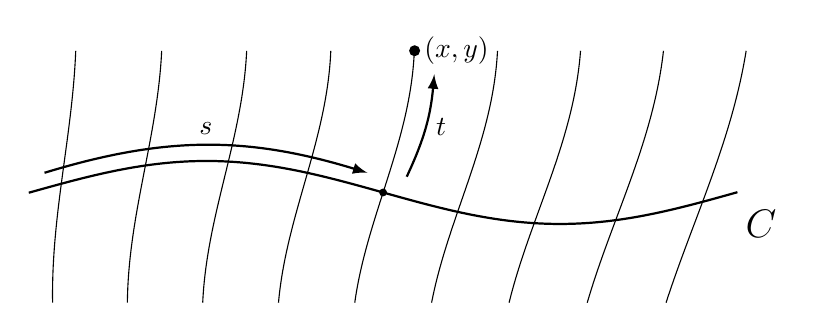
\begin{tikzpicture}[>=latex]
			\foreach \i in {-4,...,4}{
				\draw[domain=-1.4:1.8,samples=50,smooth, variable=\y] plot ({0.4*sin((0.8-0.01*\i*\i)*(\y+0.1*\i) r)+(0.03*\i)*\y+\i}, {\y});
			}
			\draw[domain=-4.5:4.5,samples=50,thick,smooth, variable=\x] plot ({\x}, {-0.4*sin(0.7*\x r)});
			\node at (4.8,-0.4) {\Large\(C\)};
			\fill[black] (0,0) circle (0.05);
			\draw[->,thick] (-4.3,0.25)to[bend left=17]node[above]{\(s\)}(-0.2,0.25);
			\draw[->,thick] (0.3,0.2)to[bend right=10]node[right]{\(t\)} (0.65,1.5);
			\fill[black] (0.4,1.8)node[right]{\((x,y)\)} circle (0.07);
		\end{tikzpicture}
	\end{figure}

	To get the solution at an arbitrary point \((x, y)\), we find the characteristic curve that goes through it and trace the solution back to the curve \(\mathcal{C}\). This will mean inverting a relationship between \((x, y)\) and \((s, t)\), where \(s\) is the coordinate along \(\mathcal{C}\) and \(t\) is the coordinate along a characteristic curve.

	We will want to make sure the vector field \(\vb{v}=(a, b)\) is not tangent to the curve \(\mathcal{C}\) on which the initial data is on, otherwise we would not be able to carry the initial data off the curve \(\mathcal{C}\) along characteristic curves to an arbitrary point \((x, y)\). If \(\vb{n}\) denotes the normal to the curve \(\mathcal{C}\), this condition is \(\vb{n}\vdot\vb{v}\ne 0\) for \((x, y)\in\mathcal{C}\). This is called the \textit{non-characteristic condition}.

	\begin{ex}
		Consider the problem
		\[\left\{\begin{aligned}
			\,&(x^2+1)\pdv{u}{x}+\pdv{u}{y}=u+1\\
			\,&u(0,y)=f(y)\,.
		\end{aligned}\right.\]
		The characteristic curves are given by
		\[\dv{x}{t}=x^2+1\quad\dv{y}{t}=1\,,\]
		with initial data on the curve
		\[(x(0),y(0))=(0,s)\,.\]
		This gives the solution
		\[\begin{cases}
			x=\tan t\\
			y=s+t\,.
		\end{cases}\]
		The \(z\)-equation is
		\[\dv{z}{t}=z+1\,,\]
		which gives the solution
		\[z=(1+z_0)e^t-1\,,\]
		where \(z_0\) is the initial value
		\[z_0=u(x_0,y_0)=u(0,s)=f(s)\,.\]
		This gives the solution
		\[z(t,s)=(1+f(s))e^t-1\,.\]
		Invert \((t,s)\rightarrow(x,y)\):
		\[\begin{cases}
			t=\arctan x\\
			s=y-\arctan x
		\end{cases}\]
		to obtain the solution
		\[u(x,y)=[1+f(y-\arctan x)]e^{\arctan x}\,.\]
	\end{ex}
	\subsection{Higher-dimensional Fourier Transform (Non-examinable)}
	\begin{defn}
		For \(f:\mathbb{R}^n\to\mathbb{C}\), its \textit{Fourier transform} is defined as
		\[\tilde{f}(\bl)\coloneqq\int e^{-i\bl\vdot\vb{x}}f(\vb{x})\dd[n]{\vb{x}}\,.\]
	\end{defn}
	\begin{thm}
		The \textit{inverse Fourier transform} is given by
		\[f(\vb{x})=\frac{1}{(2\pi)^n}\int e^{i\bl\vdot\vb{x}}\tilde{f}(\bl)\dd[n]{\bl}\,.\]
	\end{thm}
	\begin{defn}
		The convolution of two functions \(f,g:\mathbb{R}^n\to\mathbb{C}\) is
		\[(f*g)(\vb{x})\coloneqq\int f(\vb{x}-\vb{y})g(\vb{y})\dd[n]{\vb{y}}\,.\]
	\end{defn}
	\begin{thm}[The convolution theorem]
		\[\mathcal{F}_{\vb{x}\to\bl}[(f*g)(\vb{x})]=\tilde{f}(\bl)\tilde{g}(\bl)\,.\]
	\end{thm}
	\begin{prop}
		\[\mathcal{F}_{\vb{x}\to\bl}\qty[\pdv[\alpha_1]{x_1}\pdv[\alpha_2]{x_2}\dots\pdv[\alpha_n]{x_n} f(\vb{x})]=(i\lambda_1)^{\alpha_1}\dots(i\lambda_n)^{\alpha_n}\tilde{f}(\bl)\,.\]
	\end{prop}
	\subsection{Green's Function for the Heat Equation (Non-examinable)}
	\begin{defn}
		If the domain of a problem is all of \(\mathbb{R}^n\) space, then the Green's function is known as the \textit{fundamental solution}.
	\end{defn}
	We will solve the forced heat equation on \(\mathbb{R}^n\):
	\begin{equation}\tag{\(\dagger\)}
		\left\{\begin{aligned}
			&\pdv{u}{t}-\kappa\laplacian u=F(\vb{x},t) && (\vb{x},t)\in\mathbb{R}^n\times(0,\infty)\\
			&u(\vb{x},0)=f(\vb{x}) && x\in\mathbb{R}^n\,.
		\end{aligned}\right.
	\end{equation}
	We will split this problem into two parts.
	\begin{itemize}[topsep=0pt]
		\item[(a)] Zero forcing and non-zero initial data.
		\begin{equation}\tag{\(\dagger_a\)}
			\left\{\begin{aligned}
				&\pdv{u}{t}-\kappa\laplacian u=0 && (\vb{x},t)\in\mathbb{R}^n\times(0,\infty)\\
				&u(\vb{x},0)=f(\vb{x}) && x\in\mathbb{R}^n\,.
			\end{aligned}\right.
		\end{equation}
		\item[(b)] Zero initial data and non-zero forcing.
		\begin{equation}\tag{\(\dagger_b\)}
			\left\{\begin{aligned}
				&\pdv{u}{t}-\kappa\laplacian u=F(\vb{x},t) && (\vb{x},t)\in\mathbb{R}^n\times(0,\infty)\\
				&u(\vb{x},0)=0 && x\in\mathbb{R}^n\,.
			\end{aligned}\right.
		\end{equation}
	\end{itemize}
	\begin{defn}
		The \textit{heat kernel} in \(n\) dimensions is defined as
		\[K(\vb{x};t)\coloneqq\frac{1}{(4\pi\kappa t)^\frac{n}{2}}\exp[-\frac{\abs{x}^2}{4\kappa t}]\,.\]
	\end{defn}
	\begin{prop}
		For each \(t>0\), the Fourier transform of the heat kernel is
		\[\tilde{K}(\bl;t)=e^{-\kappa t\abs{\bl}^2}\,.\]
	\end{prop}
	\begin{proof}
		If
		\[g(\vb{x})=\frac{1}{(2\pi)^\frac{n}{2}}e^{-\frac{\abs{vb{x}}^2}{2}}\,,\]
		then
		\begin{align*}
			\tilde{g}(\bl)&=\int e^{-i\bl\vdot\vb{x}}g(\vb{x})\dd[n]{\vb{x}}\\
			&=\int\dd{x_1}\dots\int\dd{x_n}\qty[\frac{1}{\sqrt{2\pi}}e^{-i\lambda_1x_1-x_1^2}]\dots\qty[\frac{1}{\sqrt{2\pi}}e^{-i\lambda_nx_n-x_n^2}]\\
			&=e^{-\frac{\lambda_1^2}{2}}\dots e^{-\frac{\lambda_n^2}{2}}\\
			&=e^{-\frac{\abs{\bl}^2}{2}}\,.
		\end{align*}
		Then
		\begin{align*}
			\tilde{K}(\bl,t)&=\frac{1}{(4\pi\kappa t)^\frac{n}{2}}\int e^{-i\bl\vdot\vb{x}-\frac{\abs{\vb{x}}^2}{4\kappa t}}\dd[n]{\vb{x}}\\
			&=\frac{(2\kappa t)^\frac{n}{2}}{(4\pi\kappa t)^\frac{n}{2}}\int e^{-i(\bl\sqrt{2\kappa t})\vdot\vb{x}-\frac{\abs{\vb{x}}^2}{2}}\dd[n]{\vb{x}} & \vb{x}'=\frac{\vb{x}}{\sqrt{2\kappa t}}\,,\;\text{then drop the primes}\\
			&=\int e^{-i(\bl\sqrt{2\kappa t})\vdot\vb{x}}g(\vb{x})\dd[n]{\vb{x}}\\
			&=\tilde{g}(\bl\sqrt{2\kappa t})\\
			&=e^{-\kappa t\abs{\bl}^2}\,.
		\end{align*}\qed
	\end{proof}
	Using this result, we can find the solution to equation \((\dagger_a)\).
	\begin{prop}
		The solution to equation \((\dagger_a)\) is 
		\[u(\vb{x},t)=(K*f)(\vb{x})=\int K(\vb{x}-\vb{y},t)f(\vb{y})\dd[n]{\vb{y}}\,.\]
	\end{prop}
	\begin{proof}
		Take the Fourier transform of \((\dagger_a)\) to get
		\[\left\{\begin{aligned}
			&\pdv{\tilde{u}}{t}+\kappa\abs{\bl}^2\tilde{u}=0\\
			&\tilde{u}(\bl,0)=\tilde{f}(\bl)\,.
		\end{aligned}\right.\]
		Solving this differential equation gives
		\begin{align*}
			\tilde{u}(\bl,t)&=\tilde{u}(\bl,0)e^{-\kappa\abs{\bl}^2t}\\
			&=\tilde{f}(\bl)\tilde{K}(\bl,t)\,.
		\end{align*}
		Therefore, by the convolution theorem, \(u(\vb{x},t)=(K*f)(\vb{x})\).\qed
	\end{proof}
	\begin{prop}
		The solution to equation \((\dagger_b)\) is
		\[u(\vb{x},t)=\int_{0}^{t}\qty[\int K(\vb{x}-\vb{y},t-s)F(\vb{y},s)\dd[n]{\vb{y}}]\dd{s}\,.\]
	\end{prop}
	\begin{proof}
		Take the Fourier transform of \((\dagger_b)\) to get
		\[\left\{\begin{aligned}
			&\pdv{\tilde{u}}{t}+\kappa\abs{\bl}^2\tilde{u}=\tilde{F}(\bl,t)\\
			&\tilde{u}(\bl,0)=0\,.
		\end{aligned}\right.\]
		This differential equation is equivalent to
		\[\pdv{t}\qty[e^{\kappa\abs{\bl}^2t}\tilde{u}(\bl,t)]=e^{\kappa\abs{\bl}^2t}\tilde{F}(\bl,t)\,,\]
		and so
		\begin{align*}
			\tilde{u}(\bl,t)&=\int_{0}^{t}e^{-\kappa(t-s)\abs{\bl}^2}\tilde{F}(\bl,s)\dd{s}\\
			&=\int_{0}^{t}\tilde{K}(\bl,t-s)\tilde{F}(\bl,s)\dd{s}\,.
		\end{align*}
		The result follows from the convolution theorem.\qed
	\end{proof}
	\begin{thm}
		The solution to the heat equation in \(\mathbb{R}^n\) of the form \((\dagger)\) is
		\[u(\vb{x},t)=(K*f)(\vb{x})+\int_{0}^{t}\qty[\int K(\vb{x}-\vb{y},t-s)F(\vb{y},s)\dd[n]{\vb{y}}]\dd{s}\,.\]
	\end{thm}
	\begin{proof}
		Principle of superposition.\qed
	\end{proof}

	If we set
	\[G(\vb{x},t;\vb{y},s)=K(\vb{x}-\vb{y},t-s)H(t-s)\]
	and assume that \(F(\vb{x},t)=0\) for \(t<0\), then we can write solution to \((\dagger_b)\) as
	\[u(\vb{x},t)=\iint G(\vb{x},t;\vb{y},s)F(\vb{y},s)\dd[n]{\vb{x}}\dd{s}\,.\]
	This is the Green's function we have seen before.
	\begin{thm}
		The Green's function for the heat equation on \(\mathbb{R}^n\) with vanishing initial data is
		\begin{align*}
			G(\vb{x},t;\vb{y},s)&=K(\vb{x}-\vb{y},t-s)H(t-s)\\
			&=\left\{\begin{aligned}
				&\,\frac{1}{[4\pi\kappa(t-s)]^\frac{n}{2}}\exp[-\frac{\abs{\vb{x}-\vb{y}}^2}{4\kappa (t-s)}] && t>s\\
				&\,0 && t<s\,.
			\end{aligned}\right.
		\end{align*}
	\end{thm}
	\begin{proof}
		The Green's function should satisfy the equation
		\[\pdv{G}{t}-\kappa\laplacian G=\delta(\vb{x}-\vb{y})\delta(t-s)\,,\]
		or equivalently its Fourier transform
		\[\pdv{\tilde{G}}{t}+\kappa\abs{\bl}^2\tilde{G}=e^{-i\bl\vdot\vb{y}}\delta(t-s)\,.\]
		Our proposed Green's function has Fourier transform
		\[\tilde{G}(\bl,t;\vb{y},s)=H(t-s)\tilde{K}(\bl;t-s)e^{-i\bl\vdot\vb{y}}=H(t-s)e^{-i\bl\vdot\vb{y}}e^{-\kappa(t-s)\abs{\bl}^2}\,.\]
		This function clearly solves the Fourier transformed equation for \(t>s\) and \(t<s\).

		If we integrate the transformed equation over \((s-\epsilon,s+\epsilon)\) and take \(\epsilon\to 0\), we should require
		\[\left.\tilde{G}(\bl,t;\vb{y},s)\right|_{t=s_-}^{t=s_+}=e^{-i\bl\vdot\vb{y}}\,.\]
		This is satisfied by the proposed Green's function since
		\[\tilde{G}(\bl,s_+;\vb{y},s)=e^{-i\bl\vdot\vb{y}}\text{ and }\tilde{G}(\bl,s_-;\vb{y},s)=0\,.\]\qed
	\end{proof}
	\subsubsection{Duhamel's Principle}
	The fact that the same function \(K(\vb{x},t)\) appeared in both the solution to the homogeneous equation with inhomogeneous boundary conditions (\(\dagger_a\)), and the solution to the inhomogeneous equation with homogeneous boundary conditions (\(\dagger_b\)) is not a coincidence.

	To see this, let us return to the problem (\(\dagger_a\)) but now suppose we impose the initial condition
	\[u(\vb{x},s)=f(\vb{x})\]
	at time \(t=s\) rather than \(t=0\). A simple translation shows that for times \(t>s\), the problem is solved by
	\begin{equation}\tag{\(*_a\)}
		u(\vb{x},t)=\int K(\vb{x}-\vb{y},t-s)f(\vb{y})\dd[n]{\vb{y}}\,.
	\end{equation}
	On the other hand, the solution for the forced problem (\(\dagger_b\)) takes the form
	\begin{equation}\tag{\(*_b\)}
		u(\vb{x},t)=\int_{0}^{t}\qty[\int K(\vb{x}-\vb{y},t-s)F(\vb{y},s)\dd[n]{\vb{y}}]\dd{s}\,.
	\end{equation}
	Now suppose that for each fixed time \(t=s\), we view the forcing term \(F(\vb{y}, t)\) as an initial condition imposed at \(t=s\). The integral in square brackets above represents the effect of this condition propagated to time \(t\) as in (\(*_a\)). Finally, the time integral in (\(*_b\)) expresses the solution to the forced problem as the accumulation (superposition) of the effects from all these conditions at times \(s\) earlier than \(t\), each propagated for time interval \(t-s\) up to time \(t\). The upper limit \(t\) of this integral arose from the step function \(H(t-s)\) in the Green's function and expresses \textit{causality}: the solution at time \(t\) depends only on the cumulative effects of conditions applied at earlier times \(s<t\).

	The relation between solutions to homogeneous equations with inhomogeneous boundary conditions and inhomogeneous equations with homogeneous boundary conditions is known as \textit{Duhamel's principle}.

	\subsection{Green's Function for the Wave Equation (Non-examinable)}
	Consider the general initial value problem for the wave equation on \(\mathbb{R}^n\).
	\begin{equation}\tag{\(\dagger\)}
		\left\{\begin{aligned}
			&\,\pdv[2]{u}{t}-c^2\laplacian u=F(\vb{x},t) && (\vb{x},t)\in\mathbb{R}^n\cross(0,\infty)\\
			&\,u(\vb{x},0)=f(\vb{x}) && \vb{x}\in\mathbb{R}^n\\
			&\,\pdv{u}{t}(\vb{x},0)=g(\vb{x}) && \vb{x}\in\mathbb{R}^n\,.
		\end{aligned}\right.
	\end{equation}
	We again split the problem into two parts.
	\begin{itemize}[topsep=0pt]
		\item[(a)] Zero forcing and non-zero initial data.
		\begin{equation}\tag{\(\dagger_a\)}
			\left\{\begin{aligned}
				&\,\pdv[2]{u}{t}-c^2\laplacian u=0 && (\vb{x},t)\in\mathbb{R}^n\cross(0,\infty)\\
				&\,u(\vb{x},0)=f(\vb{x}) && \vb{x}\in\mathbb{R}^n\\
				&\,\pdv{u}{t}(\vb{x},0)=g(\vb{x}) && \vb{x}\in\mathbb{R}^n\,.
			\end{aligned}\right.
		\end{equation}
		\item[(b)] Zero initial data and non-zero forcing.
		\begin{equation}\tag{\(\dagger\)}
			\left\{\begin{aligned}
				&\,\pdv[2]{u}{t}-c^2\laplacian u=F(\vb{x},t) && (\vb{x},t)\in\mathbb{R}^n\cross(0,\infty)\\
				&\,u(\vb{x},0)=0 && \vb{x}\in\mathbb{R}^n\\
				&\,\pdv{u}{t}(\vb{x},0)=0 && \vb{x}\in\mathbb{R}^n\,.
			\end{aligned}\right.
		\end{equation}
	\end{itemize}

	We will use the function \(\Phi(\vb{x},t)\) defined implicitly by
	\[\tilde{\Phi}(\bl,t)\coloneqq\frac{\sin c\abs{\bl}t}{c\abs{\bl}}\,,\]
	and so by Fourier inversion theorem,
	\[\Phi(\vb{x},t)=\mathcal{I}_{\bl\to\vb{x}}\qty[\frac{\sin c\abs{\bl}t}{c\abs{\bl}}]=\frac{1}{(2\pi)^n}\int e^{i\bl\vdot\vb{x}}\frac{\sin c\abs{\bl}t}{c\abs{\bl}}\dd[n]{\bl}\,.\]
	The computation of this function is difficult in arbitrary dimensions. It depends on whether \(n\) is even or odd. We will consider two important cases.
	\begin{prop}
		In \(\mathbb{R}\),
		\[\Phi(\vb{x},t)=\frac{1}{2c}\qty(H(x+ct)-H(x-ct))\,.\]
	\end{prop}
	\begin{proof}
		Note that
		\[H(x+ct)-H(x-ct)=\begin{cases}
			1 & \abs{x}<ct\\
			0 & \text{otherwise}\,.
		\end{cases}\]
		It is easy to check that its Fourier transform is \(\tilde{\Phi}\).\qed
	\end{proof}
	\begin{prop}
		In \(\mathbb{R}^3\),
		\[\Phi(\vb{x},t)=\frac{1}{4\pi c}\qty[\delta(\abs{\vb{x}}-ct)-\delta(\abs{\vb{x}}+ct)]\,.\]
	\end{prop}
	\begin{proof}
		We will compute the inverse Fourier transform using spherical polar coordinates
		\[\bl=(r\sin\theta\cos\phi,r\sin\theta\sin\phi,r\cos\theta)\,.\]
		We will align the \(\lambda_3\) axis with the direction of \(\vb{x}\), so \(\vb{x}\vdot\bl=r\abs{\vb{x}}\cos\theta\). Consider
		\begin{align*}
			\int_{\abs{\bl}<R}e^{i\bl\vdot\vb{x}}\tilde{\Phi}(\bl,t)\dd[3]{\bl}&=\int_{0}^{2\pi}\dd{\phi}\int_{0}^{\pi}\dd{\theta}\int_{0}^{R}\dd{r}\frac{\sin{rct}}{rc}e^{-i\abs{\vb{x}}r\cos\theta}r^2\sin\theta\\
			&=2\pi\int_{0}^{\pi}\dd{\theta}\int_{0}^{R}\dd{r}\frac{\sin(rct)}{i\abs{\vb{x}}c}\pdv{\theta}\qty(e^{-i\abs{\vb{x}}r\cos\theta})\\
			&=2\pi\int_{0}^{R}\dd{r}\frac{\sin(rct)}{i\abs{\vb{x}}c}\qty(e^{i\abs{\vb{x}}r}-e^{-i\abs{\vb{x}}r})\\
			&=\frac{4\pi}{c\abs{\vb{x}}}\int_{0}^{R}\dd{r}\sin(rct)\sin(r\abs{\vb{x}})\,.
		\end{align*}
		The integrand is even, so we can replace \(\int_{0}^{R}\) with \(\frac{1}{2}\int_{-R}^{R}\). Using
		\[\sin A\sin B=\frac{1}{2}\qty[\cos(A-B)-\cos(A+B)]=\frac{1}{2}\Re\qty[e^{i(A-B)}-e^{i(A+B)}]\]
		gives
		\begin{align*}
			\Phi(\vb{x},t)&=\lim_{R\to\infty}\frac{1}{(2\pi)^3}\int_{\abs{\bl}}e^{i\bl\vdot\vb{x}}\tilde{\Phi}(\bl,t)\dd[n]{\lambda}\\
			&=\lim_{R\to\infty}\frac{\pi}{(2\pi)^3c\abs{\vb{x}}}\int_{-R}^{R}\dd{r}\qty(e^{ir(\abs{\vb{x}}-ct)}-e^{ir(\abs{\vb{x}}+ct)})\\
			&=\frac{\pi}{(2\pi)^3c\abs{\vb{x}}}\qty[2\pi\delta(\abs{\vb{x}}-ct)-2\pi\delta(\abs{\vb{x}}+ct)]\,,
		\end{align*}
		and the result follows.\qed
	\end{proof}
	In both cases, we can write
	\[\Phi(\vb{x},t)=\Phi^+(\vb{x},t)-\Phi^-(\vb{x},t)\,.\]
	When \(n=3\),
	\[\Phi^\pm(\vb{x},t)=\frac{\delta(\abs{\vb{x}}\mp ct)}{4\pi c\abs{\vb{x}}}\,.\]
	They are often referred to as the \textit{advanced} and \textit{retarded} parts of \(\Phi(\vb{x},t)\). 

	Note that when \(t>0\), \(\Phi^-(\vb{x},t)=0\).
	
	\begin{prop}
		The solution to \((\dagger_a)\) is given by
		\[u(\vb{x},t)=(\Phi*g)(\vb{x},t)+\pdv{t}(\Phi*f)(\vb{x},t)\,.\]
	\end{prop}
	\begin{proof}
		Taking the Fourier transform of \((\dagger_a)\) gives
		\[\left\{\begin{aligned}
			&\,\pdv[2]{\tilde{u}}{t}+c^2\abs{\bl}^2\tilde{u}=0\\
			&\,\tilde{u}(\bl,0)=\tilde{f}(\bl)\\
			&\,\pdv{\tilde{u}}{t}(\bl,0)=\tilde{g}(\bl)\,.
		\end{aligned}\right.\]
		The differential equation has a general solution
		\[\tilde{u}(\bl,t)=A(\bl)\sin(c\abs{\bl}t)+B(\bl)\cos(c\abs{\bl}t)\,,\]
		and the initial condition give
		\[B(\bl)=\tilde{f}(\bl)\,,\;A(\bl)=\frac{1}{c\abs{\bl}}\tilde{g}(\bl)\,.\]
		We have
		\[\tilde{u}(\bl,t)=\tilde{\Phi}(\bl,t)\tilde{g}(\bl)+\tilde{f}(\bl)\cos(c\abs{\bl}t)=\tilde{\Phi}(\bl,t)\tilde{g}(\bl)+\pdv{t}\qty(\tilde{\Phi}(\bl,t)\tilde{f}(\bl))\,.\]
		The result follows from the convolution theorem.\qed
	\end{proof}

	Let us focus on the term
	\[(\Phi*g)(\vb{x})=\int\Phi(\vb{y},t)g(\vb{x}-\vb{y})\dd[n]{\vb{y}}\]
	in the solution. The contribution from the advanced part, relevant for \(t>0\), in the case \(n=3\) is
	\[(\Phi^+*g)(\vb{x})=\frac{1}{4\pi c}\int\frac{\delta(\abs{y}-ct)}{\vb{y}}g(\vb{x}-\vb{y})\dd[n]{\vb{y}}=\frac{1}{4\pi c^2t}g(\vb{x}-\vb{y})\dd{S}\,.\]
	The integral is equivalent to
	\[\frac{t}{4\pi(ct)^2}\int_{\abs{\vb{x}-\vb{y}}=ct}g(\vb{y})\dd{S}=t\times\bar{g}\,,\]
	where \(\bar{g}\) is the average of \(g\) over the sphere of radius of \(ct\) centred at \(\vb{x}\).

	It turns out, in odd dimensions, this part of the solution always looks a bit like this. It always involves the spherical mean of \(g\) over a sphere of radius \(ct\) centred at \(\vb{x}\). This can be interpreted as a spherical wavefront emanating from the point \(\vb{x}\) and travelling at speed \(c\).

	In even dimensions, the solution at \((x, t)\) involves integrals over the ball \(\{\vb{y}:\abs{\vb{x}-\vb{y}}\le ct\}\).

	\begin{rem}
		These observations allow us to conclude the following very different nature of waves in an even or odd dimensional universe. In odd dimensions, if it is pitch black outside and someone flashes a torch from \(\vb{x}_0\) at time \(t=0\), you will see an instantaneous flash of light at time \(t=\frac{\abs{\vb{x}_0}}{c}\). However, in an even-dimensional world you would see a flash at \(t=\frac{\abs{\vb{x}_0}}{c}\) but it would not instantaneously disappear: instead, it would slowly fade away.
	\end{rem}
	\begin{prop}
		The solution to (\(\dagger_b\)) is
		\[u(\vb{x},t)=\int_{0}^{t}\qty[\int\Phi(\vb{x}-\vb{y},t-s)F(\vb{y},s)\dd[n]{\vb{y}}]\dd{s}\,.\]
	\end{prop}
	\begin{proof}
		Taking the Fourier transform of (\(\dagger_b\)) gives
		\[\left\{\begin{aligned}
			&\,\pdv[2]{\tilde{u}}{t}+c^2\abs{\bl}^2\tilde{u}=\tilde{F}(\bl,t)\\
			&\,\tilde{u}(\bl,0)=0\\
			&\,\pdv{\tilde{u}}{t}(\bl,0)=0\,.
		\end{aligned}\right.\]
		So we want the Green's function \(G=G(t;s)\) for the operator
		\[L=\dv[2]{t}+c^2\abs{\bl}^2\,.\]
		This is
		\[G(t;s)=\frac{\sin(c\abs{\bl}(t-s))}{c\abs{\bl}}=\tilde{\Phi}(\bl,t-s)\,.\]
		Therefore,
		\[\tilde{u}(\bl,t)=\int_{0}^{t}\tilde{\Phi}(\bl,t-s)\tilde{F}(\bl,s)\dd{s}\,,\]
		and the result follows from the convolution theorem.\qed
	\end{proof}

	\begin{thm}
		The solution to the wave equation in \(\mathbb{R}^n\) of the form \((\dagger)\) is
		\[u(\vb{x},t)=(\Phi*g)(\vb{x},t)+\pdv{t}(\Phi*f)(\vb{x},t)+\int_{0}^{t}\qty[\int\Phi(\vb{x}-\vb{y},t-s)F(\vb{y},s)\dd[n]{\vb{y}}]\dd{s}\,.\]
	\end{thm}
	\begin{proof}
		Principle of superposition.\qed
	\end{proof}

	Like the heat equation, if we define \(F(\vb{x},t)=0\) for \(t<0\) and introduce the function
	\[G(\vb{x},t;\vb{y},s)=H(t-s)\Phi(\vb{x}-\vb{y},t-s)\,,\]
	then the solution to (\(\dagger_b\)) can be written as
	\[u(\vb{x},t)=\iint G(\vb{x},t;\vb{y},s)F(\vb{y},s)\dd[n]{\vb{y}}\dd{s}\,.\]

	We call \(G\) the Green's function for the Wave equation on \(\mathbb{R}^n\) with vanishing initial data. It satisfies
	\[\pdv[2]{G}{t}-c^2\laplacian G=\delta(\vb{x}-\vb{y},t-s)\,.\]

	\subsection{Green's Function for the Laplacian}
	\begin{lem}
		A 1D real Green's function is symmetric.
		\[G(x;\xi)=G(\xi;x)\,.\]
	\end{lem}
	\begin{proof}
		\[G(x;\xi)=\sum_{n=1}^{\infty}\frac{1}{\lambda_n}y_n(x)y_n^*(\xi)\,,\]
		where \(\lambda_n\) and \(y_n\) are the eigenvalues and eigenfunctions of the differential operators. It is obvious that for real \(y(x)\), 
		\[G(x;\xi)=G(\xi;x)\,.\]\qed
	\end{proof}
	\begin{cor}
		Real Green's function is symmetric.
		\[G(\vb{x};\vb{y})=G(\vb{y};\vb{x})\,.\]
	\end{cor}

	To find the Green's function of the Laplacian on a bounded domain \(\Omega\) with Dirichlet boundary conditions, we would naturally require
	\[\begin{cases}
		\laplacian G(\vb{x};\vb{y})=\delta(\vb{x}-\vb{y}) & \vb{x}\in\Omega\\
		G(\vb{x};\vb{y})= 0 & \vb{x}\in\partial\Omega\,.
	\end{cases}\]

	However, if we are solving Poisson's equation with Neumann boundary conditions, then instead of requiring \(\pdv{G}{n}=0\) on \(\partial\Omega\), we can only require
	\[\pdv{G}{n}\equiv\vb{n}(r)\vdot\grad G=\frac{1}{A}\text{ on }\partial\Omega\,,\]
	where \(A=\oint_{\partial\Omega}\dd{S}\) is the surface area. This is because a zero flux on the boundary is impossible. 
	\begin{proof}
		\begin{align*}
			\oint_{\partial\Omega}\grad G\vdot\vb{n}\dd{S}&=\int_\Omega\laplacian G\dd{V}\\
			&=\int_\Omega\delta(\vb{x}-\vb{y})\dd{V}=1\,.
		\end{align*}\qed
	\end{proof}
	\begin{rem}
		However, when the domain \(\Omega\) is the whole \(\mathbb{R}^n\) space, we still require \(\pdv{G}{n}=0\) since \(A\to\infty\).
	\end{rem}

	We are interested in the Green's function for the \(\mathbb{R}^n\) space with Dirichlet boundary conditions, also known as the fundamental solutions, such that
	\[\begin{cases}
		\laplacian G(\vb{x};\vb{y})=\delta(\vb{x}-\vb{y})\\
		\abs{G(\vb{x};\vb{y})}\to 0 \text{ as }\abs{x}\to\infty\,.
	\end{cases}\]
	Taking the Fourier transform of the equation gives
	\[\tilde{G}(\bl;\vb{y})=-\frac{e^{-i\bl\vdot\vb{y}}}{\abs{\bl}^2}\,.\]
	We need the following result.
	\begin{prop}
		For \(\alpha>0\) and \(\vb{x}\in\mathbb{R}^n\), we have
		\[\mathcal{F}_{\vb{x}\to\bl}[\abs{\vb{x}}^{-\alpha}]=C_{n,\alpha}\abs{\bl}^{\alpha-n}\,.\]
	\end{prop}
	\begin{proof}
		Let \(f_\alpha(\vb{x})=\abs{\vb{x}}^{-\alpha}\), we have
		\[\tilde{f}_\alpha(\bl)=\int\abs{\vb{x}}^{-\alpha}e^{-i\bl\vdot\vb{x}}\dd[n]{\vb{x}}\,.\]
		If we make a change of variables \(\vb{x}=\mathsf{R}\tp\vb{x}'\), where \(\mathsf{R}\) is a rotation matrix, then since \(\det{\mathsf{R}}=1\), after dropping the primes, we have
		\begin{align*}
			\tilde{f}_\alpha(\bl)&=\int\abs{\mathsf{R}\tp\vb{x}}^{-\alpha}e^{-i\bl\vdot(\mathsf{R}\tp\vb{x})}\dd[n]{\vb{x}}\\
			&=\int\abs{\vb{x}}^{-\alpha}e^{-i(\mathsf{R}\bl)\vdot\vb{x}}\dd[n]{\vb{x}}=\tilde{f}_\alpha(\mathsf{R}\bl)\,.
		\end{align*}
		Therefore, \(\tilde{f}_\alpha\) is rotation invariant. We can just write \(\bl=\abs{\bl}\vb{u}\) for any unit vector \(\vb{u}\), and the result will not depend on the direction of \(\vb{u}\). Making the substitution \(\vb{x}'=\abs{\bl}\vb{x}\) and dropping primes we get
		\begin{align*}
			\tilde{f}_\alpha(\bl)&=\int\abs{\vb{x}}^{-\alpha}e^{-i\abs{\bl}(\vb{m}\vdot\vb{x})}\dd[n]{\vb{x}}\\
			&=\abs{\lambda}^{-n}\int\abs{\bl}^\alpha\abs{\vb{x}}^{-\alpha}e^{-i(\vb{m}\vdot\vb{x})}\dd[n]{\vb{x}}=C_{n,\alpha}\abs{\bl}^{\alpha-n}\,,
		\end{align*}
		where \(C_{n,\alpha}\) is only dependent on \(n\) and \(\alpha\).\qed
	\end{proof}
	If \(n>2\), set \(\alpha=n-2\), there is a constant \(c_n\) such that
	\[\frac{1}{\abs{\bl}^2}=c_n\mathcal{F}_{\vb{x}\to\bl}\qty[\abs{\vb{x}}^{2-n}]\,.\]
	\begin{thm}
		The free space Green's function for the Laplacian on \(\mathbb{R}^n\) with \(n>2\) is
		\[G(\vb{x};\vb{y})=-\frac{1}{(n-2)\norm{S^{n-1}}}\times\frac{1}{\abs{\vb{x}-\vb{y}}^{n-2}}\,,\]
		where \(\norm{S^{n-1}}\) is the surface area of an \(n-1\) sphere, given by
		\[\norm{S_{n-1}}=\frac{2\pi^{\frac{n}{2}}}{\Gamma(\frac{n}{2})}\,.\]
		In particular, for \(n=3\),
		\[G(\vb{x};\vb{y})=-\frac{1}{4\pi}\frac{1}{\abs{\vb{x}-\vb{y}}}\,.\]
	\end{thm}
	\begin{proof}
		Let \(F(\vb{x})=c_n\abs{\vb{x}}^{2-n}\), then
		\[\tilde{G}(\bl;\vb{y})=-e^{-i\bl\vdot\vb{y}}\tilde{F}(\vb{\lambda})=-\mathcal{F}_{\vb{x}\to\bl}[F(\vb{x}-\vb{y})]\,.\]
		Therefore,
		\[G(\vb{x};\vb{y})=-\frac{c_n}{\abs{\vb{x}-\vb{y}}^{n-2}}\,.\]
		To find \(c_n\), note that
		\[-\laplacian(\abs{\vb{x}}^{2-n})=\frac{\delta(\vb{x})}{c_n}\,,\]
		so integrating over \(\abs{\vb{x}}\le 1\) and using the divergence theorem gives
		\[\frac{1}{c_n}=-\int_{\abs{\vb{x}}=1}\grad(\abs{\vb{x}}^{2-n})\vdot\dd{\vb{S}}=(n-2)\int_{\abs{\vb{x}}=1}\dd{S}=(n-2)\times\norm{S^{n-1}}\,.\]\qed
	\end{proof}
	We need to use a different method to obtain the Green's function in \(\mathbb{R}^2\).
	\begin{prop}
		For \(\mathbb{R}^2\), the Green's function for the Laplacian is given by
		\[G(\vb{x};\vb{y})=\frac{1}{2\pi}\ln\abs{\vb{x}-\vb{y}}+C\,.\]
	\end{prop}
	\begin{proof}
		By translation invariance of the Laplacian, it is enough to consider the case \(\vb{y}=\vb{0}\). For \(\vb{y}=\vb{0}\), we have \(\abs{\vb{x}}=r\), so
		\begin{align*}
			\laplacian G&=\frac{1}{2\pi}\laplacian\ln r\\
			&=\frac{1}{2\pi}\frac{1}{r}\pdv{r}\qty(r\pdv{r}\ln r)=0\,.
		\end{align*}
		We need to check that what happens at \(\vb{x}=\vb{0}\). By the divergence theorem, for any \(\epsilon>0\),
		\begin{align*}
			\int_{\abs{\vb{x}}<\epsilon}\laplacian\ln r \dd[2]\vb{x}&=\int_{\abs{\vb{x}}=\epsilon}\grad\ln r\vdot\dd{\vb{S}}\\
			&=\int_{0}^{2\pi}\frac{\vb{e}_r}{\epsilon}\vdot\vb{e}_r\epsilon\dd{\theta}=2\pi\,.
		\end{align*}
		We have \(\laplacian\ln\abs{\vb{x}}=0\) for all \(\abs{\vb{x}}\ne 0\) and
		\[\int_{\abs{\vb{x}}<\epsilon}\laplacian\ln\abs{\vb{x}}\dd[2]{\vb{x}}=2\pi\]
		for any \(\epsilon>0\). Therefore
		\[\laplacian\ln\abs{\vb{x}}=2\pi\delta(\vb{x})\]
		and so
		\[G(\vb{x};\vb{y})=\frac{1}{2\pi}\ln\abs{\vb{x}-\vb{y}}+C\,.\]\qed
	\end{proof}
	\begin{rem}
		It is impossible for the 2D Green's function to vanish at \(\vb{x}\to\infty\). We can control the finite \(\vb{x}\) at which \(G\) vanishes by adjusting the arbitrary constant \(C\).
	\end{rem}
	\subsection{The Method of Images}
	Now we are using the method of images to find the Green's function of laplacian on a domain \(\Omega\) that is not the full \(\mathbb{R}^n\) space.
	\subsubsection{3D Half Space}
	Suppose that we want to find the Green's function for a domain \(\Omega\) with Dirichlet boundary conditions, where \(\Omega\) is the half-space of \(\mathbb{R}^3\) with \(z>0\).

	The Green's function satisfies
	\[\begin{cases}
		\laplacian G=\delta(\vb{x}-\vb{y}) & \text{for }\vb{x}\in\Omega\\
		G=0 & \text{on }z=0\\
		G=0 & \text{as }\abs{\vb{x}}\to\infty\,,\;\vb{x}\in\Omega\,.
	\end{cases}\]

	The uniqueness of the solution allows us to solve this using a trick: remove the boundary at \(z=0\), consider all of space and add a point source of opposite sign, an \textit{image source}, at the image point \(\vb{y}'=(x',y',-z')\).

	The Green's function satisfies
	\[\laplacian G=\delta(\vb{x}-\vb{y})-\delta(\vb{x}-\vb{y}')\,,\]
	which, by superposition of the fundamental solutions, gives
	\[G(\vb{x};\vb{y})=-\frac{1}{4\pi\abs{\vb{x}-\vb{y}}}+\frac{1}{4\pi\abs{\vb{x}-\vb{y}'}}\,.\]
	We can check that this solution satisfies all the conditions, and therefore, by the uniqueness of the solution, Green's function is
	\[G(\vb{x};\vb{y})=-\frac{1}{4\pi}\qty(\frac{1}{\abs{\vb{x}-\vb{y}}}-\frac{1}{\abs{\vb{x}-\vb{y}'}})\,.\]

	If instead we impose Neumann boundary conditions at \(z=0\):
	\[\pdv{G}{n}=\pdv{G}{z}=0\text{ at }z=0\,,\]
	and still require \(G\to 0\) as \(\abs{\vb{x}}\to\infty\), \(\vb{x}\in\Omega\), then we need a point charge of the same sign at the image point. The Green's function is
	\[G(\vb{x};\vb{y})=-\frac{1}{4\pi}\qty(\frac{1}{\abs{\vb{x}-\vb{y}}}+\frac{1}{\abs{\vb{x}-\vb{y}'}})\,.\]
	
	\subsubsection{2D Quarter Plane}
	Suppose now we want to find Green's function for a domain \(\Omega\) with Dirichlet boundary conditions, where \(\Omega\) is the quarter plane of \(\mathbb{R}^2\) with \(x>0\), \(y>0\).

	The Green's function now satisfies
	\[\begin{cases}
		\laplacian G=\delta(\vb{x}-\vb{y}_1) & \text{for }\vb{x}\in\Omega\\
		G=0 & \text{on }x=0\\
		G=0 & \text{on }y=0\\
		G=0 & \text{as }\abs{\vb{x}}\to\infty\,,\;\vb{x}\in\Omega\,.
	\end{cases}\]
	We then need three image charges: two of the opposite sign at \(\vb{y}_2=(-x_0,y_0)\), \(\vb{y}_3=(x_0,-y_0)\) and one of the same sign at \(\vb{y}_4=(-x_0,-y_0)\).
	By superposition of the fundamental solutions, we have
	\[G(\vb{x};\vb{y}_0)=\frac{1}{2\pi}\ln\frac{\abs{\vb{x}-\vb{y}_1}\abs{\vb{x}-\vb{y}_4}}{\abs{\vb{x}-\vb{y}_2}\abs{\vb{x}-\vb{y}_3}}\,.\]

	\subsubsection{Sphere}
	Suppose now we want to find the Green's function for a domain \(\Omega:\abs{\vb{x}}<a\) in \(\mathbb{R}^3\), under Dirichlet boundary conditions.

	The Green's function satisfies
	\[\begin{cases}
		\laplacian G=\delta(\vb{x}-\vb{y}) & \text{for }\vb{x}\in\Omega\\
		G=0 & \text{for }\abs{\vb{x}}=a\,.
	\end{cases}\]

	The image source would be of the strength \(-\frac{a}{\abs{\vb{y}}}\) at the \textit{inverse point} of the source
	\[\vb{y}'=\frac{a^2}{\abs{\vb{y}}^2}\vb{y}\,.\]
	The Green's function is therefore
	\[G(\vb{x};\vb{y})=-\frac{1}{4\pi}\qty(\frac{1}{\abs{\vb{x}-\vb{y}}}-\frac{a}{\abs{\vb{y}}\abs{\vb{x}-\vb{y}'}})\,.\]

	\begin{proof}
		at \(\abs{\vb{x}}=a\),
		\begin{align*}
			\abs{\vb{x}-\vb{y}'}&=\sqrt{\abs{\vb{x}}^2+\abs{\vb{y}'}^2-2\vb{x}\vdot\vb{y}'}\\
			&=\sqrt{a^2+\frac{a^4}{\abs{\vb{y}}^2}-2\frac{a^2}{\abs{\vb{y}}^2}\vb{x}\vdot\vb{y}}\\
			&=\frac{a}{\abs{\vb{y}}}\sqrt{\abs{\vb{y}}^2+a^2-2\vb{x}\vdot\vb{y}}\\
			&=\frac{a}{\abs{\vb{y}}}\abs{\vb{x}-\vb{y}}\,.
		\end{align*}
		Therefore, \(G(\vb{x};\vb{y})=0\) at the boundary \(\abs{\vb{x}}=a\).\qed
	\end{proof}
	\subsubsection{Circle}
	Suppose now we want to find the Green's function for a domain \(\Omega:\abs{\vb{x}}<a\) in \(\mathbb{R}^2\), under Dirichlet boundary conditions.

	The image point is the inverse point again, with \(\vb{y}'=\frac{a^2}{\abs{\vb{y}}^2}\vb{y}\), but now the image just needs to have the strength \(-1\) as we are able to adjust the constant \(C\). The Green's function is
	\[G(\vb{x};\vb{y})=\frac{1}{2\pi}\ln\frac{\abs{\vb{x}-\vb{y}}}{\abs{\vb{x}-\vb{y}'}}+C\,,\]
	where the constant \(C\) is chosen to ensure that \(G=0\) on the circle \(\abs{\vb{x}}=a\).

	\subsection{The Integral Solution of Poisson's Equation}
	To find the solution of Poisson's equation with an arbitrary source distribution, we will need Green's identity.

	\begin{thm}[Green's first identity]
		Suppose \(\Omega\subset\mathbb{R}^n\) is a compact set with boundary \(\partial\Omega\), and let \(\phi,\psi:\Omega\to\mathbb{R}\) be a pair of functions on \(\Omega\) that are regular throughout \(\Omega\).
		\[\int_\Omega\phi\laplacian\psi+(\grad\phi)\vdot(\grad\psi)\dd{V}=\int_{\partial\Omega}\phi\grad\psi\vdot\vb{n}\dd{S}\,,\]
		where \(\vb{n}\) is the outward pointing normal to \(\partial\Omega\).
	\end{thm}
	\begin{proof}
		Apply product rule and divergence theorem.
		\begin{align*}
			\int_\Omega\div(\phi\grad\psi)\dd{V}&=\int_\Omega\phi\laplacian\psi+(\grad\phi)\vdot(\grad\psi)\dd{V}\\
			&=\int_{\partial\Omega}\phi\grad\psi\vdot\vb{n}\dd{S}\,.
		\end{align*}\qed
	\end{proof}

	\begin{thm}[Green's second identity]		
		Suppose \(\Omega\subset\mathbb{R}^n\) is a compact set with boundary \(\partial\Omega\), and let \(\phi,\psi:\Omega\to\mathbb{R}\) be a pair of functions on \(\Omega\) that are regular throughout \(\Omega\).
		\[\int_\Omega\phi\laplacian\psi-\psi\laplacian\phi\dd{V}=\oint_{\partial\Omega}(\phi\grad\psi-\psi\grad\phi)\vdot\vb{n}\dd{S}\eqqcolon\oint_{\partial\Omega}\phi\pdv{\psi}{n}-\psi\pdv{\phi}{n}\dd{S}\,.\]
	\end{thm}
	\begin{proof} 
		Interchange \(\phi\) and \(\psi\) in the Green's first identity to obtain
		\[\int_\Omega\psi\laplacian\phi+(\grad\psi)\vdot(\grad\phi)\dd{V}=\int_{\partial\Omega}\psi\grad\phi\vdot\vb{n}\dd{S}\,,\]
		then subtract from the Green's first identity.\qed
	\end{proof}
	\begin{rem}
		We will apply the Green's second identity to the fundamental solution. However, \(G(\vb{x},\vb{y})\) is singular at \(\vb{y}\) so it is not clear whether the identity is valid, because the divergence theorem usually requires functions to be regular throughout \(\Omega\).
	\end{rem}
	
	Consider Poisson's equation in a domain \(\Omega\) with inhomogeneous Dirichlet boundary conditions:
	\begin{equation}\tag{\(\dagger\)}
		\left\{\begin{aligned}
			&\,\laplacian\phi=\rho(\vb{x}) && \vb{x}\in\Omega\\
			&\,\phi(\vb{x})=f(\vb{x}) && \vb{x}\in\partial\Omega\,.
		\end{aligned}\right.
	\end{equation}
	We will first directly apply Green's identity with \(\psi=G\) in a less rigorous way, which gives
	\[\int_\Omega(\phi\laplacian G-G\laplacian\phi)\dd{V}=\oint_{\partial\Omega}(\phi\grad G-G\grad\phi)\vdot\vb{n}\dd{S}\]
	\[\implies \int_\Omega(\phi\delta(\vb{x}-\vb{y})-G\rho(\vb{x}))\dd{V}=\oint_{\partial\Omega}(f(\vb{x})\grad G-0\times\grad\phi)\vdot\vb{n}\dd{S}\]
	\[\implies \int_\Omega\phi(\vb{x})\delta(\vb{x}-\vb{y})\dd{V}=\int_\Omega\rho(\vb{x})G(\vb{x};\vb{y})\dd{V}+\oint_{\partial\Omega}f(\vb{x})(\grad G\vdot\vb{n})\dd{S}\,.\]

	\begin{thm}\label{intpoi}
		The integral solution of the Poisson's equation in domain \(\Omega\) with Dirichlet boundary condition
		\begin{equation}\tag{\(\dagger\)}
			\left\{\begin{aligned}
				&\,\laplacian\phi=\rho(\vb{x}) && \vb{x}\in\Omega\\
				&\,\phi(\vb{x})=f(\vb{x}) && \vb{x}\in\partial\Omega
			\end{aligned}\right.
		\end{equation}
		is given by
		\[\phi(\vb{y})=\int_\Omega\rho(\vb{x})G(\vb{x};\vb{y})\dd{V}+\oint_{\partial\Omega}f(\vb{x})\pdv{G(\vb{x};\vb{y})}{n}\dd{S}\,.\]
	\end{thm}
	\begin{proof}[Non-examinable]
		Here is the formal proof. To remove the singularity issues of the Green's function, consider a ball \(B_\epsilon\) of radius \(\epsilon\ll 1\) centred at the singular point \(\vb{x}=\vb{y}\). Let \(\Omega'\) be the region
		\[\Omega'=\Omega-B_\epsilon\,.\]
		Now the Green's function is perfectly regular everywhere in \(\Omega'\), so we can apply Green's second identity with \(\psi=G\) to get
		\begin{align*}
			\int_{\Omega'}\phi\laplacian G-G\laplacian\phi\dd{V}&=-\int_{\Omega'}G\rho(\vb{x})\dd{V}\\
			&=\int_{\partial\Omega'}\phi\grad G\vdot\vb{n}-G\grad\phi\vdot\vb{n}\dd{S}\\
			&=\int_{\partial\Omega}\phi\grad G\vdot\vb{n}\dd{S}+\int_{S_{\epsilon}^{n-1}}\phi\grad G\vdot\vb{n}-G\grad\phi\vdot\vb{n}\dd{S}\,,
		\end{align*}
		where the first equality follows since \(\laplacian G=0\) in \(\Omega'\). Note that on the inner boundary, a sphere of radius \(\epsilon\), the outward-pointing unit normal is \(\vb{n} = -\vu{r}\). As \(\epsilon\to 0\), the Green's function approaches the fundamental solution so
		\[G|_{S_{\epsilon}^{n-1}}=-\frac{1}{(n-2)\norm{S_{\epsilon}^{n-1}}}\frac{1}{\epsilon^{n-2}}\,,\]
		\[\vb{n}\vdot\grad G|_{S_{\epsilon}^{n-1}}=-\frac{1}{\norm{S^{n-1}}}\frac{1}{\epsilon^{n-1}}\,.\]
		The measure on an \((n-1)\)-sphere of radius \(\epsilon\) is \(\dd{S}=\epsilon^{n-1}\dd{\Omega_n}\), where \(\dd{\Omega_n}\) is an integral over angles. Therefore, we have
		\[-\int_{S_{\epsilon}^{n-1}}G\grad\phi\vdot\vb{n}\dd{S}=\frac{\epsilon}{\norm{S_{\epsilon}^{n-2}}}\int\vb{n}\vdot\grad\phi\dd{\Omega_n}\,.\]
		Since \(\phi\) is regular at \(\vb{y}\), the value of this integral is bounded, so this term vanishes as \(\epsilon\to 0\). Also,
		\[\int_{S_{\epsilon}^{n-1}}\phi\grad G\vdot\vb{n}\dd{S}=-\frac{1}{\norm{S_{\epsilon}^{n-1}}}\int\phi\dd{\Omega_n}=-\bar{\phi}\,,\]
		where \(\bar{\phi}\) is the average value of \(\phi\) on the sphere surrounding \(\vb{y}\). As \(\epsilon\to 0\), this \(\bar{\phi}\to\phi(\vb{y})\). Putting all these together we find that, as \(\epsilon\to 0\) so that \(\Omega'=\Omega\),
		\[\phi(\vb{y})=\int_{\Omega}G\rho(\vb{x})\dd{V}+\int_{\partial\Omega}\phi\grad G\vdot\vb{n}\dd{S}\,.\]
		This is the result as claimed.\qed
	\end{proof}
	If we want \(\Omega\) to be all space, we can use the fundamental solution for \(G\) but we need to ensure that the surface integral \(\to 0\).
	\begin{cor}
		The solution to the Poisson's equation on all space:
		\[\left\{\begin{aligned}
			&\,\laplacian\phi=\rho(\vb{x}) && \vb{x}\in\mathbb{R}^n\\
			&\,\phi(\vb{x})=0 && \abs{\vb{x}}\to\infty
		\end{aligned}\right.\]
		is given by
		\[\phi(\vb{y})=\int_\Omega\rho(\vb{x})G(\vb{x};\vb{y})\dd{V}\,.\]
	\end{cor}
	\begin{cor}
		The solution to the Laplace's equation
		\[\left\{\begin{aligned}
			&\,\laplacian\phi=0 && \vb{x}\in\Omega\\
			&\,\phi(\vb{x})=f(\vb{x}) && \vb{x}\in\partial\Omega
		\end{aligned}\right.\]
		is given by
		\[\phi(\vb{y})=\oint_{\partial\Omega}f(\vb{x})\pdv{G(\vb{x};\vb{y})}{n}\dd{S}\,.\]
	\end{cor}

	An integral solution of Poisson's equation with Neumann boundary conditions
	\[\left\{\begin{aligned}
		&\,\laplacian\phi=\rho(\vb{x}) && \vb{x}\in\Omega\\
		&\,\pdv{\phi}{n}=f(\vb{x}) && \vb{x}\in\partial\Omega
	\end{aligned}\right.\]
	can also be derived. From Green's identity
	\[\int_\Omega(\phi\laplacian G-G\laplacian\phi)\dd{V}=\oint_{\partial\Omega}(\phi\grad G-G\grad\phi)\vdot\vb{n}\dd{S}\,,\]
	we have
	\[\phi(\vb{y})=\int_\Omega\rho(\vb{x})G(\vb{x},\vb{y})\dd{V}+\frac{1}{A}\oint_{\partial\Omega}\phi(\vb{x})\dd{S}-\oint_{\partial\Omega}f(\vb{x})G(\vb{x};\vb{y})\dd{S}\,.\]
	\begin{thm}
		The integral solution of the Poisson's equation over full \(\Omega=\mathbb{R}^n\) domain with Neumann boundary condition
		\begin{equation}\tag{\(\dagger\)}
			\left\{\begin{aligned}
				&\,\laplacian\phi=\rho(\vb{x}) && \vb{x}\in\Omega\\
				&\,\pdv{\phi}{n}=f(\vb{x}) && \vb{x}\in\partial\Omega
			\end{aligned}\right.
		\end{equation}
		is given by
		\[\phi(\vb{y})=\int_\Omega\rho(\vb{x})G(\vb{x};\vb{y})\dd{V}-\oint_{\partial\Omega}f(\vb{x})G(\vb{x};\vb{y})\dd{S}\,.\]
		as long as the surface integral over \(\phi\) is finite.
	\end{thm}
	\begin{rem}
		The solution also works with finite \(\Omega\) and \({\partial\Omega}\) although it contains an integral of the unknown \(\Phi\) because this is essentially a constant term. Since we are dealing with a problem with Neumann boundary conditions, the solution is determined up to an unknown constant and such an integral term will not affect our result. In a problem with the Neumann boundary condition, we only care about \(\grad\phi\).
	\end{rem}

	\begin{ex}
		Solve the electric potential \(\phi\) of a charged wire of length \(2L\) with charged density \(\mu\) per unit length, lying along the \(z\) axis from \(z=-L\) to \(z=L\).
		
		We have the Poisson's equation
		\[\laplacian\phi=\rho(\vb{x})\]
		with
		\[\rho(\vb{x})=\begin{cases}
			\frac{\mu}{\epsilon_0}\delta(\vb{x}) & \text{for }-L\le z\le L\\
			0 & \text{otherwise}\,.
		\end{cases}\]
		The Green's function is the fundamental solution, so the integral solution is
		\begin{align*}
			\phi(\vb{y})&=\int_{\mathbb{R}^3}\frac{\rho(\vb{x})}{4\pi\epsilon_0\abs{\vb{x}-\vb{y}}}\dd[3]{\vb{x}}\\
			&=\frac{\mu}{4\pi\epsilon_0}\int_{-L}^{L}\dd{z}\iint\frac{\delta(\vb{x})}{\abs{\vb{x}-\vb{y}}}\dd{x}\dd{y}\\
			&=\frac{\mu}{4\pi\epsilon_0}\int_{-L}^{L}\frac{\dd{z}}{\sqrt{x'^2+y'^2+(z-z')^2}}\,,
		\end{align*}
		which, after a substitution of \(z-z'=\sqrt{x'^2+y'^2}\sinh u\) and relabelling, gives
		\[\phi=\frac{\mu}{4\pi\epsilon_0}\qty[\sinh^{-1}\frac{L-z}{\sqrt{x^2+y^2}}+\sinh^{-1}\frac{L+z}{\sqrt{x^2+y^2}}]\,.\]
	\end{ex}

	\begin{ex}
		\textit{Solution of Laplace's equation in 3D half space.}
		
		Find the solution of Laplace's equation in the 3D half-space with \(z>0\) subject to the Dirichlet boundary condition \(\phi=f(x,y)\) on \(z=0\).

		\(\Omega\) it the half-space, and the bounding surface \({\partial\Omega}\) is the \(z=0\) plus the hemisphere at \(\infty\). We can neglect the hemisphere at \(\infty\) since \(\phi\to 0\) there. Hence, the integral solution is given by
		\[\phi(\vb{y})=\oint_{\partial\Omega}f(\vb{x})\pdv{G}{n}\dd{S}\,.\]

		The Green's function, derived previously using the method of image, is
		\[G(\vb{x},\vb{y})=-\frac{1}{4\pi}\qty(\frac{1}{\abs{\vb{x}-\vb{y}}}-\frac{1}{\abs{\vb{x}-\vb{z}}})\,.\]
		We have
		\begin{align*}
			\left.\pdv{G}{z}\right|_{z=0}&=-\frac{1}{4\pi}\pdv{z}\left\{\frac{1}{\sqrt{(x-x')^2+(y-y')^2+(z-z')^2}}\right.\\
			&\qquad\qquad\qquad-\left.\left.\frac{1}{\sqrt{(x-x')^2+(y-y')^2+(z+z')^2}}\right\}\right|_{z=0}\\
			&=-\frac{z'}{2\pi[(x-x')^2+(y-y')^2+z'^2]^\frac{3}{2}}\dd{x}\dd{y}\,,
		\end{align*}
		and so
		\[\phi(\vb{y})=\frac{z'}{2\pi}\int_{-\infty}^{\infty}\int_{-\infty}^{\infty}\frac{f(x,y)}{[(x-x')^2+(y-y')^2+z'^2]^\frac{3}{2}}\dd{x}\dd{y}\,.\]
	\end{ex}
	
	\newpage
	
	\section{Group Theory}
	\subsection{Mappings}
	These alternative terminologies are common when talking about groups.
	\begin{defn}
		A map \(f:X\rightarrow Y\) is \textit{one-to-one} (injective) if \(f(x_1)=f(x_2)\) implies \(x_1=x_2\). \(f\) maps distinct elements to distinct elements.
	\end{defn}
	\begin{defn}
		A map \(f:X\rightarrow Y\) is \textit{onto} (surjective) if for every \(y\in Y\), there is at least one \(x\in X\) such that \(f(x)=y\).
	\end{defn}
	\subsection{Groups}
	\begin{defn}
		A \textit{group} is a triple \((G,\,\cdot\,,I)\) of a set \(G\), a binary operation \(\cdot\) on \(G\), and an element \(I\in G\) such that the following axioms are satisfied:
		\begin{enumerate}[topsep=0pt,parsep=0.5em]
			\item[(G0)] \textit{Closure.} \(\forall g_1,\, g_2\in G, \, g_2\cdot g_1\in G\);
			\item[(G1)] \textit{Associativity.} \(\forall g_1,\, g_2,\, g_3\in G,\, g_3\cdot(g_2\cdot g_1)=(g_3\cdot g_2)\cdot g_1\);
			\item[(G2)] \textit{Identity.} \(\exists I\in G\) such that \(\forall g\in G,\,g\cdot I=I\cdot g=g\);
			\item[(G3)] \textit{Inverse.} \(\forall g\in G,\,\exists g^{-1}\in G\) such that \(g\cdot g^{-1}=g^{-1}\cdot g=I\).
		\end{enumerate}
	\end{defn}
	\begin{rems}
		\begin{itemize}[topsep=0pt]
			\item Sometimes axiom G0 is not stated since it is implied in the definition of binary operations.
			\item It is common to abbreviate the group \((G,\,\cdot\,,I)\) as \(G\), and group product \(g_2\cdot g_1\) as \(g_2g_1\).
			\item A set of elements with two binary operations can form more complicated algebraic structures, including \textit{rings} and \textit{fields}.
		\end{itemize}
	\end{rems}
			
	\begin{defn}
		A set \(R\) together with two binary operations and two identities, one for each operation, \((R,+,e,\cdot,u)\), is a \textit{ring} if elements in \(R\) satisfy the ring axioms:
		\begin{enumerate}[topsep=0pt,parsep=0.5em]
			\item[(R0)] \textit{Closure.} \(\forall a,\, b\in R,\, a+b,\,a\cdot b\in R\);
			\item[(R1)] \textit{Associativity.} \(\forall a,\, b,\, c\in R,\, a+(b+c)=(a+b)+c,\,a\cdot(b\cdot c)=(a\cdot b)\cdot c\);
			\item[(R2)] \textit{Additive commutativity.} \(\forall a,\,b\in R,\,a+b=b+a\);
			\item[(R3)] \textit{Distributivity.} \(\forall a,\,b,\,c\in R,\, a\cdot(b+c)=a\cdot b+a\cdot c\), \((a+b)\cdot c=a\cdot c+b\cdot c\);
			\item[(R4)] \textit{Additive identity.} \(\exists e\in R\) such that \(\forall a\in R,\,e+a=a\);
			\item[(R5)] \textit{Multiplicative identity.} \(\exists u\in R,\,u\ne e\) such that \(\forall a\in R,\,u\cdot a=a\cdot u=a\);
			\item[(R6)] \textit{Additive inverse.} \(\forall a\in R,\,\exists b\in R\) such that \(a+b=e\).
		\end{enumerate}
	\end{defn}
	\begin{defn}
		A ring \(\mathbb{F}\) is a \textit{field} if it is commutative in multiplication and any non-zero element has a multiplicative inverse:
		\begin{enumerate}[topsep=0pt,parsep=0.5em]
			\item[(F7)] \textit{Multiplicative commutativity.} \(\forall a,b\in \mathbb{F},\,a\cdot b=b\cdot a\).
			\item[(F8)] \textit{Multiplicative inverse.} \(\forall a\in \mathbb{F},\,a\ne e,\,\exists b\in \mathbb{F}\) such that \(a\cdot b=u\).
		\end{enumerate}
	\end{defn}
	\begin{rem}
		Common fields include \(\mathbb{Q}\), \(\mathbb{R}\) and \(\mathbb{C}\) under addition and multiplication.
	\end{rem}

	\begin{prop}
		The identity of a group is unique.
	\end{prop}
	\begin{proof}
		Assume group \(G\) has two distinct identities \(I,\, I'\), then
		\[II'=I=I'\,,\]
		which contradicts our assumption.\qed
	\end{proof}
	
	\begin{prop}
		A group element's inverse is unique.
	\end{prop}
	\begin{proof}
		Assume some \(g\in G\) has two distinct inverses \(h,\, k\), then
		\[gh=I\text{ and }kg=I\]
		\[\implies\;(kg)h=k(gh)=kI=k\]
		\[\implies\;Ih=k \text{ so }h=k\,,\]
		which contradicts our assumption.\qed
	\end{proof}
	
	\begin{prop}
		The inverse of a product is given by
		\[(g_2g_1)^{-1}=g_{1}^{-1}g_{2}^{-1}\,.\]
	\end{prop}
	\begin{proof}
		\begin{align*}
			g_{1}^{-1}g_{2}^{-1}g_2g_1&=g_{1}^{-1}Ig_1\\
			&=g_1^{-1}g_1\\
			&=I\,.
		\end{align*}\qed
	\end{proof}
	
	\subsubsection{Commutativity and Order}
	\begin{defn}
		A group \((G,\cdot,I)\) is \textit{Abelian} if for all \(g_1,g_2\in G\), we have \(g_1g_2=g_2g_1\). Otherwise, the group is \textit{non-Abelian}.
	\end{defn}
	\begin{defn}
		A group is \textit{finite} if it contains a finite number of elements. The \textit{order} of a finite group is the number of elements it contains, denoted as \(\abs{G}\).
		
		An \textit{infinite group} has infinitely many elements.
	\end{defn}
	\begin{defn}
		The \textit{order} of a group element \(g\in G\) is the least integer \(q\) such that \(g^q=I\). For any finite group,
		\[q\le\abs{G}\,.\]
	\end{defn}
	
	\subsection{Symmetry of the Square}
	Groups arise naturally in the study of symmetries. Let us first consider an \(n\)-gon lying on the complex plane \(\mathbb{C}\).
	\begin{defn}
		An \textit{isometry} is a rigid motion or transformation which preserves distances between points.
	\end{defn}

	Let set \(D_n\) consist of the isometries of \(\mathbb{C}\) that send the \(n\)-gon to itself. If \(f,g:\mathbb{C}\to\mathbb{C}\) are isometries that send the \(n\)-gon to itself, then so is the composition \(f\circ g\), so \(\circ\) defines a binary operation on \(D_n\). Let \(I\in D_n\) be the isometry \(I(x)=x\).
	\begin{thm}
		\((D_n,\circ,I)\) is a group, called the \(n^\text{th}\) dihedral group. It has order \(2n\).
	\end{thm}
	\begin{rem}
		Most pure mathematicians will confusingly denote this group as \(D_{2n}\), based on its order.
	\end{rem}

	\begin{figure}[ht!]
		\centering
		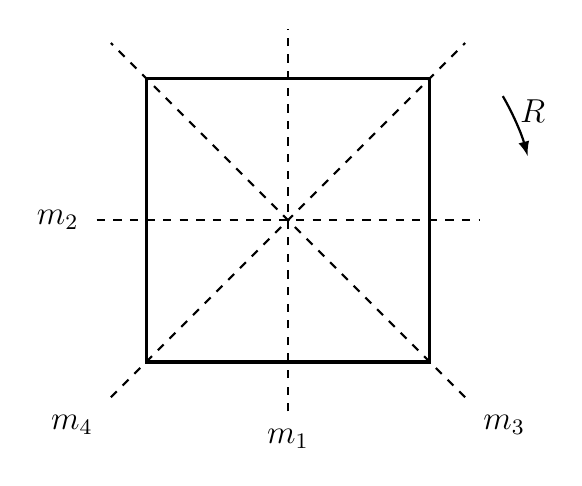
\begin{tikzpicture}[>=latex,scale=0.9]
			\draw[very thick] (-2,-2) rectangle (2,2);
			\draw[thick,dashed] (-2.7,0)node[left=1mm]{\large\(m_2\)}--(2.7,0);
			\draw[thick,dashed] (0,-2.7)node[below=1mm]{\large\(m_1\)}--(0,2.7);
			\draw[thick,dashed] (-2.5,-2.5)node[below left=1mm]{\large\(m_4\)}--(2.5,2.5);
			\draw[thick,dashed] (2.5,-2.5)node[below right=1mm]{\large\(m_3\)}--(-2.5,2.5);
			\draw[thick,->] (3.031,1.75) arc (30:15:3.5);
			\node at (3.45,1.54) {\large\(R\)};
		\end{tikzpicture}
	\end{figure}

	Let us consider the group of transformations which represent the symmetries of the square.	Let rotations of \(0^\circ\), \(90^\circ\), \(180^\circ\), \(270^\circ\) anticlockwise be \(I\), \(R\), \(R^2\), \(R^3\) respectively. Let reflections under four axes of symmetry be \(m_1\), \(m_2\), \(m_3\), \(m_4\) respectively.
	
	This is then the \textit{4-fold dihedral group}, \(D_4\). This is an example of a \textit{point group}, for which the operations leave one point fixed.
	
	Each reflection is its own inverse:
	\[m_1^2=m_2^2=m_3^2=m_4^2=I\,,\]
	and for rotations,
	\[RR^3=R^2R^2=R^4=I\,.\]
	
	\begin{defn}
		There is a minimal subset from which all other group elements can be obtained by composition. We say the group is \textit{generated} by such a subset, and the members of the subset are called the \textit{generators} of the group.
	\end{defn}
	\begin{ex}
		For instance, the subset \(\{R,m_1\}\) generates the group as follows:
		\[\{I,\, R,\, R^2,\, R^3,\, m_1,\, m_2,\, m_3,\, m_4\}=\{R^4,\, R,\, R^2,\, R^3,\, m_1,\, R^2m_1,\, R^3m_1,\, Rm_1\}\,.\]
	\end{ex}
	
	\subsubsection{Group Table}
	We can construct a table for all \(g_2g_1\), where \(g_1\) are on the top row and \(g_2\) are on the leftmost column. For the \(D_4\) group, the group table is:
	
	\begin{center}
		\begin{TAB}(b,25pt,13pt)[3pt]{c|ccccccc}{c|ccccccc}
		\(I\)	& \(R^2\) & \(R\) & \(R^3\) & \(m_1\) & \(m_2\) & \(m_3\) & \(m_4\) \\
		\(R^2\) & \(I\) & \(R^3\) & \(R\) & \(m_2\) & \(m_1\) & \(m_4\) & \(m_3\) \\
		\(R\)	& \(R^3\) & \(R^2\) & \(I\) & \(m_4\) & \(m_3\) & \(m_1\) & \(m_2\) \\
		\(R^3\) & \(R\) & \(I\) & \(R^2\) & \(m_3\) & \(m_4\) & \(m_2\) & \(m_1\) \\
		\(m_1\) & \(m_2\) & \(m_3\) & \(m_4\) & \(I\) & \(R^2\) & \(R\) & \(R^3\) \\
		\(m_2\) & \(m_1\) & \(m_4\) & \(m_3\) & \(R^2\) & \(I\) & \(R^3\) & \(R\) \\
		\(m_3\) & \(m_4\) & \(m_2\) & \(m_1\) & \(R^3\) & \(R\) & \(I\) & \(R^2\) \\
		\(m_4\) & \(m_3\) & \(m_1\) & \(m_2\) & \(R\) & \(R^3\) & \(R^2\) & \(I\)
		\end{TAB}
	\end{center}

	By observing the group table, we can notice that each row and column is a complete rearrangement of the group elements. This is the rearrangement theorem.
	
	\begin{thm}[Rearrangement theorem]\label{reargthm}
		Let \(G=\{g_1,\dots,g_n\}\) be a group, then \(\forall g\in G\),
		\[gG=\{gg_1,\dots,gg_n\}\]
		contains each element of the group once and only once.
	\end{thm}
	\begin{proof}
		\(\forall g_\alpha\in G,\,\exists g_\beta\in G\) such that \(gg_\beta=g_\alpha\) (just let \(g_\beta=g^{-1}g_\alpha)\), so \(gG\) contains all elements in \(G\).
		
		Also, the set \(gG\) has no repeated element, since if \(gg_\beta=gg_\beta'\), then
		\[g^{-1}gg_\beta=g^{-1}gg_\beta'\implies g_\beta=g_\beta'\,.\]\qed
	\end{proof}
	\begin{cor}
		We also have that, \(\forall g\in G\),
		\[Gg=\{g_ig\mid g_i\in G\}=G\,.\]
	\end{cor}
	
	\subsubsection{Subgroups}
	\begin{defn}
		Let \((G,\cdot,I)\) be a group and \(H\subseteq G\), then \((H,\cdot,I)\) is a \textit{subgroup} of \(G\), denoted \(H\le G\) if
		\begin{enumerate}[topsep=0pt]
			\item \(I\in H\);
			\item for all \(h_1,h_2\in H\), \(h_1\cdot h_2\in H\);
			\item \((H,\cdot,I)\) is a group.
		\end{enumerate}
		A subgroup \(H\le G\) is \textit{proper} if \(H\ne\{I\}\) and \(H\ne G\). 
	\end{defn}
	\begin{rem}
		To exclude the case that \(H=G\), we use \(H<G\).
	\end{rem}
	\begin{ex}
		\textit{Proper subgroups of \(D_4\).}
		
		By examining the group table of \(D_4\), we can spot 5 order-2 subgroups:
		\[\{I,\, R^2\},\, \{I,\, m_1\},\, \{I,\, m_2\},\, \{I,\, m_3\},\, \{I,\, m_4\}\,, \]
		and an order-4 cyclic subgroup, \(C_4\):
		\[\{I,\, R,\, R^2,\, R^3\}\,.\]
		In addition, there are two other order-4 subgroups:
		\[\{I,\, R^2,\, m_1,\, m_2\}\text{ and } \{I,\, R^2,\, m_3,\, m_4\}\,,\]
		which are called \textit{Klein four-group} or \textit{Vierergruppe}, denoted by \(K_4\) or \(V_4\).
	\end{ex}
	\subsubsection{Cyclic Groups}
	\begin{defn}
		A \textit{cyclic group} is a group \(G\) that can be generated by a single group element \(g\). A finite cyclic group of order \(n\) is denoted as \(C_n\).
	\end{defn}
	A finite cyclic group of order \(n\) contains group members
	\[\{I,\, g,\, g^2,\dots,\, g^{n-1}\}\,,\]
	and it follows that \(I=g^n\).
	\subsection{Homomorphism}
	\begin{defn}
		If \((H,\cdot_H,I_H)\) and \((G,\cdot_G,I_G)\) are groups then a function \(\phi : H \to G\) is called a \textit{homomorphism} if for all \(a,b\in H\), we have
		\[\phi(a\cdot_H b)=\phi(a)\cdot_G\phi(b)\,.\]
	\end{defn}
	\begin{rem}
		A homomorphism is a map between groups that preserves group operations but is not necessarily 1-1 or onto.
	\end{rem}

	\begin{defn}
		If \(\phi : H\to G\) is a homomorphism, then
		\begin{itemize}[topsep=0pt]
			\item the \textit{image} of \(\phi\) is
			\[\Im(\phi)\coloneqq \{ g\in G\mid g=\phi(h)\text{ for some }h\in H\}\,.\]
			\item the \textit{kernel} of \(\phi\) is
			\[\ker(\phi)\coloneqq \{ h\in H\mid \phi(h)=I_G\}\,.\]
		\end{itemize}
	\end{defn}
	\begin{lem}\label[lem]{homidinv}
		If \(\phi: H\to G\) is a homomorphism, then
		\begin{enumerate}[topsep=0pt]
			\item \(\phi(I_H)=I_G\),
			\item for all \(h\in H\), we have \(\phi(h^{-1})=\phi(h)^{-1}\).
		\end{enumerate}
	\end{lem}
	\begin{proofskip}
		\begin{enumerate}[topsep=0pt]
			\item
			\[\phi(I_H)\cdot_G\phi(I_H)=\phi(I_H\cdot_H I_H)=\phi(I_H)\]
			\[\implies\quad\phi(I_H)=I_G\,.\]
			\item
			\[\phi(h)\cdot_G\phi(h^{-1})=\phi(h\cdot_H h^{-1})=\phi(I_H)=I_G\]
			\[\phi(h^{-1})\cdot_G\phi(h)=\phi(h^{-1}\cdot_H h)=\phi(I_H)=I_G\]
			These are the defining properties of \(\phi(h)^{-1}\), so \(\phi(h^{-1})=\phi(h)^{-1}\).\qed
		\end{enumerate}
	\end{proofskip}
	
	\begin{ex}
		Let \(G=(\mathbb{R}\),+,0) and \(G'=U(1)\), the multiplicative group of unit-magnitude complex numbers. Define a mapping \(\phi:\,\mathbb{R}\rightarrow U(1)\) such that for \(x\in \mathbb{R}\),
		\[\phi(x)=e^{ix}\,.\]
		This is a homomorphism because
		\[\phi(x+y)=e^{i(x+y)}=e^{ix}e^{iy}=\phi(x)\phi(y)\,.\]
		The kernel of \(\phi\) is \(\ker(\phi)=\{2N\pi\mid N\in\mathbb{Z}\}=\{\dots,\, -2\pi,\, 0,\, 2\pi,\dots\}\)
	\end{ex}
	\begin{prop}\label[prop]{kersubgroup}
		If \(\phi: H\to G\) is a homomorphism, then \(\Im(\phi)\le G\) and \(\ker(\phi)\le H\).
	\end{prop}
	\begin{proof}
		We have \(\phi(I_H)=I_G\in\Im(\phi)\). \(\Im(\phi)\) is closed because for any \(g_1=\phi(h_1), g_2=\phi(h_2)\in \Im(\phi)\), \(g_1g_2=\phi(h_1 h_2)\in \Im(\phi)\). Also, the inverse exists for all elements in \(\Im(\phi)\) by \cref{homidinv}.

		We have \(I_H\in\ker(\phi)\). If \(h_1,\, h_2\in\ker(\phi)\), then \(h_1h_2\in\ker(\phi)\) since it must be mapped to \(I_G\). Also, if \(h\in\ker(\phi)\), then \(h^{-1}\in \ker(\phi)\) since \(\phi(h^{-1})=(\phi(h))^{-1}=I_G^{-1}=I_G\), so \(\ker(\phi)\le H\).\qed
	\end{proof}
	\begin{defn}
		If a homomorphism \(\phi: H\to G\) is invertible then it is an \textit{isomorphism}, written \(G\cong H\).
	\end{defn}
	\begin{rem}
		Two groups are usually considered identical if there is an isomorphism between them.
	\end{rem}
	The following theorem is useful for checking whether a homomorphism is an isomorphism.

	\begin{thm}
		If \(\phi: H \to G\) is a homomorphism, then it is an isomorphism if and only if \(\Im(\phi) = G\) and \(\ker(\phi) = {I_H}\).
	\end{thm}
	\subsection{Group Actions (Non-examinable)}
	We motivated our definition of a group \(G\) as the symmetries of an object \(X\), but when defining a group we abstracted the properties that symmetries of an object have and there was no longer an \(X\).

	It is now the time to take the object that our groups acting on back.

	\begin{defn}
		An action of a group \((G,\,\cdot\,, I)\) on a set \(X\) is a function \( * : G\times X \to X\) satisfying
		\begin{enumerate}[topsep=0pt]
			\item[(A1)] \textit{Identity.} For all \(x \in X\) we have \(I*x=x\).
			\item[(A2)] \textit{Associativity.} For all \(a,b\in G\) and \(x\in X\) we have \((a\cdot b)*x=a*(b*x)\).
		\end{enumerate}
	\end{defn}
	\begin{exs}
		\begin{enumerate}[topsep=0pt]
			\item Any group acts on any set by the \textit{trivial action} \(g*x=x\).
			\item Any group acts on the set \(X=G\) by the \textit{left regular action} \(g*g'=g\cdot g'\) and the \textit{right regular action} \(g*g'=g'\cdot g\).
			\item The dihedral group acts on the set of vertices of the regular \(n\)-gon.
		\end{enumerate}
	\end{exs}
	\begin{defn}
		Let \(G\) act on \(X\). The \textit{orbit} of \(x\in X\) is the set
		\[G*x\coloneqq \{y\in X\mid y=g*x\text{ for some }g\in G\}\,.\]
		The \textit{stabiliser} of \(x\in X\) is
		\[G_x\coloneqq\{g\in G\mid g*x=x\}\,.\]
	\end{defn}
	\begin{thm}[Orbit-stabiliser theorem]
		Let a finite group \(G\) act on a set \(X\).
		\[\abs{G}=\abs{G_x}\abs{G*x}\,.\]	
	\end{thm}

	\begin{defn}
		The \textit{symmetric group} of a set \(X\), \(\mathrm{Sym}(X)\) is the group whose elements are all the bijection functions from the set to itself \(\phi: X\to X\), and whose group operation is the composition of functions.
	\end{defn}
	\begin{thm}\label{actionthm}
		The action \(*\) of a group \(G\) on a set \(X\) is the same as the homomorphism
		\begin{align*}
			\rho:G&\to\mathrm{Sym}(X)\\
			g&\mapsto t_g\,,
		\end{align*}
		where \(t_g\) is the function
		\begin{align*}
			t_g:X&\to X\\
			x&\mapsto g*x\,.
		\end{align*}
	\end{thm}
	\begin{thm}[Cayley's theorem]\label{caythm}
		Any group is isomorphic to a subgroup of some symmetric group.
	\end{thm}
	\begin{proof}
		Consider the left regular action of \(G\) on the set \(X=G\). By the construction in \cref{actionthm}, this corresponds to a homomorphism \(\rho:G\to\mathrm{Sym}(G)\). The image \(\Im(\rho)\) of \(\rho\) is a subgroup of \(\mathrm{Sym}(G)\), and we may consider as a homomorphism \(\rho:G\to\Im(\rho)\). If \(g\in\ker(\rho)\) then \(g*h=h\) for all \(h\in G\), but as \(g*h=g\cdot h\) it then follows that \(g = I\), so \(\ker(\rho)=\{I\}\). It then follows that \(\rho:G\to\Im(\rho)\) is an isomorphism, so G is isomorphic to \(\Im(\rho)\), which is a subgroup of \(\mathrm{Sym}(G)\).\qed
	\end{proof}
	
	\subsection{Cosets and Lagrange's Theorem}
	\subsubsection{Cosets}
	\begin{defn}
		A \textit{left coset} of a subgroup \(H\le G\) is an orbit of the right regular action of \(H\) on \(G\). We write \(G/ H\) for the set of orbits of this action, and call it \textit{the set of left cosets}. If \(g\in G\) then its left coset is
		\[gH\coloneqq\{g'\in G\mid g'=gh\text{ for some }h\in H\}\,.\]

		A \textit{right coset} of \(H\le G\) is an orbit of the left regular action of \(H\) on \(G\), and we write \(H\backslash G\) for \textit{the set of right cosets}.
	\end{defn}
	
	\begin{prop}
		For a subgroup \(H\) of an Abelian group \(G\), the left coset \(gH\) and the right coset \(Hg\) are identical.
	\end{prop}
	\begin{proof}
		Trivial by the definition of Abelian groups.\qed
	\end{proof}
	\begin{prop}\label[prop]{cosetpar}
		A subgroup \(H\) of \(G\) and its left (or right) cosets partition \(G\).
	\end{prop}
	\begin{proofskip}
		\begin{enumerate}[topsep=0pt,parsep=1em]
			\item Two cosets are either disjoint or equal.
			
			Suppose \(g_1 H\) and \(g_2 H\) have one element in common: \(g_1 h_1=g_2 h_2\). Then
			\[g_1 H=g_2 h_2 h_1^{-1} H = g_2H\]
			since \(h_2 h_1^{-1}\in H\). So if there is one element in common, the cosets are identical.
			\item Two cosets \(g_1 H\) and \(g_2 H\) are identical if and only if \(g_1^{-1}g_2\in H\).
			
			If \(g_1^{-1} g_2=h\in H\), then
			\[g_1 H=g_1 h H = g_1 g_1^{-1} g_2 H = g_2 H\,.\]
			Conversely, if \(g_1 H=g_2 H\),
			\[H=g_1^{-1} g_2 H\,,\]
			so \(g_1^{-1} g_2 h\in H\) \(\forall h\in H\), so \(g_1^{-1} g_2\in H\).
			\item Every element of \(G\) is in some coset.
			
			Since \(H\) contains \(I\), then for any element \(g\in G\), the coset \(g H\) contains \(g\).\qed
		\end{enumerate}
	\end{proofskip}
	
	\subsubsection{Lagrange's Theorem}
	\begin{thm}[Lagrange's theorem]	
		Let \(G\) be a finite group and let \(H\le G\), then
		\[\abs{G}=n\abs{H},\quad n\in\mathbb{Z}\,.\]
	\end{thm}
	\begin{proof}
		This follows immediately from \cref{cosetpar}.\qed
	\end{proof}
	\begin{cor}
		The order of every element of \(G\) also divides \(\abs{G}\).
	\end{cor}
	\begin{proof}
		Any \(g\in G\) generates a cyclic subgroup of \(G\).\qed
	\end{proof}
	\begin{prop}
		Any group of prime order is cyclic.
	\end{prop}
	\begin{proof}
		Let \(G\) be a group of order \(p\), where \(p\) is a prime number, and \(g\in G\), \(g\ne I\). Consider the subgroup \(H\) of \(G\) generated by \(g\), which must be a cyclic group with order greater than 1. By Lagrange's theorem, a subgroup of \(G\) can only have order 1 or \(p\), so the group generated by \(g\) must be \(G\) itself, and so \(G\) is cyclic.\qed
	\end{proof}
	\subsection{Conjugacy Class}
	\subsubsection{Conjugacy Class}
	\begin{defn}
		Two group elements \(g_1, g_2\in G\) are \textit{conjugate} to each other if there exists some group element \(g\) such that
		\[g_2=gg_1g^{-1},\;\text{or equivalently}\; g_2g=gg_1\,.\]
		The \textit{conjugate action} of \(G\) on a subgroup \(H\le G\) is
		\[g*h\coloneqq ghg^{-1}\,.\]
	\end{defn}
	\begin{defn}
		An \textit{equivalence relation} is a binary relationship between elements of a set, written \(g_1\sim g_2\), which satisfies
		\begin{enumerate}[topsep=0pt]
			\item \textit{Reflexivity}: \(g_1\sim g_1\).
			\item \textit{Symmetry}: \(g_1\sim g_2\) implies \(g_2\sim g_1\).
			\item \textit{Transitivity}: If \(g_1\sim g_2\) and \(g_2\sim g_3\), then \(g_1\sim g_3\).
		\end{enumerate}
	\end{defn}
	
	\begin{prop}
		Conjugacy is an equivalence relation.
	\end{prop}
	\begin{proofskip}
		\begin{enumerate}[topsep=0pt]
			\item Choose \(g=I\).
			\[g_1=Ig_1I^{-1}\,.\]
			\item Suppose that \(g_2=gg_1g^{-1}\), then for \(g'=g^{-1}\),
			\[g_1=g'g_2g'^{-1}\,.\]
			\item If \(g_2=g_ag_1g_a^{-1}\) and \(g_3=g_bg_2g_b^{-1}\), then
			\[g_3=gg_1g^{-1}\,,\]
			where \(g=g_bg_a\).\qed
		\end{enumerate}
	\end{proofskip}
	\begin{defn}
		The conjugacy relation partitions any group \(G\) into disjoint equivalence classes called \textit{conjugacy classes}. Elements in the same class are conjugate, and elements in different classes are not.
	\end{defn}
	\begin{prop}
		For a group \(G\),
		\begin{enumerate}[topsep=0pt]
			\item For any \(g\in G\), \(a\in G\), \(gag^{-1}\) is in the same conjugacy class as \(a\).
			\item The identity of any group is a conjugacy class by itself.
			\item Each element of an Abelian group is in a class by itself.
		\end{enumerate}
	\end{prop}
	\begin{proofskip}
		\begin{enumerate}[topsep=0pt]
			\item Trivial by definition.
			\item For any \(g\in G\),
			\[gIg^{-1}=gg^{-1}=I\,.\]
			\item For any \(g_1\), \(g_2\) in an Abelian group \(G\),
			\[g_2g_1g_2^{-1}=g_2g_2^{-1}g_1=g_1\,,\]
			so \(g_1\) can only be a conjugacy class by itself.\qed
		\end{enumerate}
	\end{proofskip}
	\begin{ex}
		\textit{Conjugacy classes of \(D_4\).}
		\begin{center}
			\begin{TAB}(b,25pt,13pt)[3pt]{c|c|cc|cc|cc}{c|c|cc|cc|cc}
				\(I\)	& \(R^2\) & \(R\) & \(R^3\) & \(m_1\) & \(m_2\) & \(m_3\) & \(m_4\) \\
				\(R^2\) & \(I\) & \(R^3\) & \(R\) & \(m_2\) & \(m_1\) & \(m_4\) & \(m_3\) \\
				\(R\)	& \(R^3\) & \(R^2\) & \(I\) & \(m_4\) & \(m_3\) & \(m_1\) & \(m_2\) \\
				\(R^3\) & \(R\) & \(I\) & \(R^2\) & \(m_3\) & \(m_4\) & \(m_2\) & \(m_1\) \\
				\(m_1\) & \(m_2\) & \(m_3\) & \(m_4\) & \(I\) & \(R^2\) & \(R\) & \(R^3\) \\
				\(m_2\) & \(m_1\) & \(m_4\) & \(m_3\) & \(R^2\) & \(I\) & \(R^3\) & \(R\) \\
				\(m_3\) & \(m_4\) & \(m_2\) & \(m_1\) & \(R^3\) & \(R\) & \(I\) & \(R^2\) \\
				\(m_4\) & \(m_3\) & \(m_1\) & \(m_2\) & \(R\) & \(R^3\) & \(R^2\) & \(I\)
			\end{TAB}
		\end{center}
		
		The 5 conjugacy classes are:
		\[\{I\},\,\{R^2\},\,\{R,\, R^3\},\,\{m_1,\, m_2\},\,\{m_3,\, m_4\}\,.\]
	\end{ex}
	\subsubsection{Normal Subgroup}
	\begin{defn}
		A subgroup \(H\) of \(G\) is a \textit{normal subgroup} if for every \(h\in H\), \(g\in G\),
		\[ghg^{-1}\in H\,.\]
		We write \(H\unlhd G\) to mean \(H\) is a normal subgroup of \(G\), and \(H\lhd G\) to exclude \(H=G\).

		The normal subgroup \(H\unlhd G\) is \textit{proper} if it is not \(\{I\}\) or \(G\).
	\end{defn}
	
	\begin{rem}
		A normal subgroup consists of complete conjugacy classes of the group.
	\end{rem}
	
	\begin{prop}
		Any subgroup of an Abelian group is normal.
	\end{prop}
	\begin{proof}
		Let \(H\) be a subgroup of an Abelian group \(G\). For all \(g\in G\) and \(h\in H\) we have
		\[ghg^{-1}=gg^{-1}h=h\,.\]\qed
	\end{proof}
	\begin{prop}
		The left and right cosets of \(H\) are identical if and only if \(H\unlhd G\).
	\end{prop}
	\begin{proof}
		\[gHg^{-1}=H\quad\iff\quad gH=Hg\,.\]\qed
	\end{proof}
	\begin{prop}\label[prop]{kernormsub}
		If \(\phi: H\to G\) is a homomorphism, then \(\ker(\phi)\unlhd H\).
	\end{prop}
	\begin{proof}
		We have \(\ker(\phi)\le H\) by \cref{kersubgroup}. \(\ker(\phi)\) is normal in \(H\) since for \(k\in\ker(\phi)\) and \(h\in H\),
		\[\phi(hkh^{-1})=\phi(h)\phi(k)\phi(h^{-1})=\phi(h)I_G\phi(h)^{-1}=I_G\,,\]
		so \(hkh^{-1}\in\ker(\phi)\).\qed
	\end{proof}
	
	\subsubsection{Quotient Groups}
	We can try to define a group operation on the cosets of \(H\le G\) by
	\[(g_1H)\cdot(g_2 H)\coloneqq (g_1g_2)H\,,\]
	but we must be worried about where this is well-defined: the same coset may be represented by many elements of G, and we must show that the answer obtained does not depend on which representative of each coset we choose.

	If \(g_1H=g_1'H\) and \(g_2H=g_2'H\), then we must have \(g_1=g_1'h_1\) and \(g_2'=g_2h_2\). Then
	\[g_1'g_2'H=g_1h_1g_2h_2H=g_1h_1g_2H=g_1g_2(g_2^{-1}h_1g_2)H\,,\]
	which is equal to \(g_1g_2H\) (for which the product is therefore well-defined) if and only if \(g_2^{-1}h_1g_2\in H\) holds for all \(g_2\in G\) and \(h_1\in H\). Therefore, \(H\) must be normal in \(G\).

	\begin{thm}\label{qgthm}
		If \(H\) is a normal subgroup of \(G\), then
		\[(g_1H)\cdot(g_2H)\coloneqq g_1g_2H\]
		is a well-defined binary operation on the set \(G/H\) of left cosets, and \((G/H,\cdot,IH)\) is a group.
	\end{thm}
	\begin{proof}
		The binary operation is well-defined, as shown above. The associativity is satisfied since
		\begin{align*}
			(g_1H\cdot g_2H)\cdot g_3H&=(g_1g_2 H)\cdot g_3H\\
			&=(g_1g_2g_3)H\\
			&=g_1H\cdot(g_2H\cdot g_3H)\,.
		\end{align*}
		The identity is \(IH\) since \(gH\cdot IH=(g\cdot I)H=gH\), and we also have the inverse: \(gH\cdot g^{-1}H=(g\cdot g^{-1})H=IH\). \((G/H,\cdot,IH)\) is a well-defined group.\qed
	\end{proof}
	\begin{defn}
		If \(H\) is a normal subgroup of \(G\), then the quotient group is the set \(G / H\) of left cosets with the group structure described in \cref{qgthm}.
	\end{defn}
	\begin{thm}[The first isomorphism theorem]\label{isothm}
		Let \(\phi: G\to H\) be a homomorphism. Then the mapping
		\begin{align*}
			\rho: G/\ker(\phi)&\to\Im(\phi)\\
			g\ker(\phi)&\mapsto\phi(g)
		\end{align*}
		is well-defined and is a group isomorphism.
	\end{thm}
	\begin{proof}
		From \cref{kernormsub}, \(\ker(\phi)\unlhd G\), so we have a quotient group \(G / \ker(\phi)\).

		If \(g\ker(\phi)=g'\ker(\phi)\), then \(g'=gk\) for some \(k\in\ker(\phi)\). Thus
		\begin{align*}
			\phi(g')&=\phi(g\cdot k)\\
			&=\phi(g)\cdot\phi(k)\\
			&=\phi(g)\cdot I=\phi(g)\,,
		\end{align*}
		and hence \(\rho(g\ker(\phi))=\rho(g'\ker(\phi))\), which means that \(\rho\) is well-defined.

		We have
		\begin{align*}
			\rho(a\ker(\phi)\cdot b\ker(\phi))&=\rho(ab\ker(\phi))\\
			&=\phi(a)\cdot\phi(b)\\
			&=\rho(a\ker(\phi))\cdot\rho(b\ker(\phi))\,,
		\end{align*}
		so \(\rho\) is a homomorphism,

		The function \(\rho\) is surjective, as the set \(\Im(\phi)\) consists, by definition, of the elements of the form \(\phi(g)\). If \(\rho(a\ker(\phi))=I_H\) then \(\phi(a)=I_H\), so \(a\in\ker(\phi)\), but then \(a\ker(\phi)=I_G\ker(\phi)\). Thus the kernel of \(\rho\) is \(\{I_G \ker(\phi)\}\), so \(\rho\) is injective, and is therefore an isomorphism.\qed
	\end{proof}
	\begin{ex}
		Consider a homomorphism \(\phi: D_3\to C_2\), where
		\[\{I_D,R,R^2,m_1,m_2,m_3\}\mapsto\{I_C,I_C,I_C,a,a,a\}.\]
		The kernel of \(\phi\) is
		\[K=\{I_D,R,R^2\}=C_3\,.\]
		We can check that \(D_3/C_3\) is isomorphic to \(C_2\).
	\end{ex}

	\subsection{The Permutation Groups}
	\subsubsection{Permutation Groups and Permutations}
	\begin{defn}	
		The \textit{finite symmetric group}, or the \textit{permutation group}, \(\mathrm{S}_{n}\), is the symmetric group of a finite set of \(n\) elements.
	\end{defn}
	\begin{prop}
		The order of a permutation group \(S_n\) is
		\[\abs{S_n}=n!\,.\]
	\end{prop}
	\begin{prop}
		For \(n>1\), \(S_{n-1}\) is a subgroup of \(S_n\).
	\end{prop}
	\begin{rem}
		Just think of leaving the \(n^{\text{th}}\) element fixed and permuting the other \(n-1\) elements.
	\end{rem}
	Since a permutation is a bijection of a set to itself, it can be represented using the following convention.
	\begin{defn}
		\textit{Cauchy's two-line notation} is a notation of permutations putting each element in the first row and its image below in the second row. If \(\sigma\in S_n\) is a permutation of the set \(X=\{x_1,x_2,...,x_n\}\), then
		\[\sigma=\begin{pmatrix}
			x_1 & x_2 & \dots & x_n\\
			\sigma(x_1) & \sigma(x_2) & \dots & \sigma(x_n)
		\end{pmatrix}\,.\]
	\end{defn}
	\begin{rem}
		The inverse permutation is easily found by swapping the two rows.
		\[\sigma^{-1}=\begin{pmatrix}
			\sigma(x_1) & \sigma(x_2) & \dots & \sigma(x_n)\\
			x_1 & x_2 & \dots & x_n
		\end{pmatrix}\,.\]
	\end{rem}
	\begin{rem}
		We can omit the columns referring to the unchanged objects, and swap the order of any columns.
	\end{rem}
	\begin{ex}
		\[\begin{pmatrix}
			2 & 3 & 1 & 4 & 5\\
			3 & 1 & 2 & 4 & 5
		\end{pmatrix}\equiv\begin{pmatrix}
			2 & 3 & 1\\
			3 & 1 & 2
		\end{pmatrix}\equiv\begin{pmatrix}
			1 & 2 & 3\\
			2 & 3 & 1
		\end{pmatrix}\,.\]
	\end{ex}
	\begin{defn}
		For a permutation group \(S_n\) acting on a set of objects \(X=\{a_i\}_{i=1}^{n}\), a \(k\)-cycle
		\[(a_1~a_2~\dots~a_k)\in S_n\,,\]
		on the elements \(a_1,a_2,\dots,a_k\in\{x_1,x_2,\dots,x_n\}\) is the permutation given by
		\[\begin{pmatrix}
			a_1 & a_2 & \dots & a_k\\
			a_2 & a_3 & \dots & a_1
		\end{pmatrix}\,.\]
	\end{defn}
	\begin{rem}
		Remember that \(\sigma\in S_n\) is a bijection function acting on a set \(X\).

		For example, let \(a_1,a_2,\dots,a_k\in\{1,2,\dots,n\}\), then the \(k\) cycle
		\[(a_1~a_2~\dots ~a_k)(i)=\begin{cases}
			a_{j+1} & \text{if }i=a_j\text{ for }j<k\\
			a_1 & \text{if }i=a_k\\
			i & \text{if }i\ne a_j \text{ for any } j\,.
		\end{cases}\]
	\end{rem}
	\begin{lemskip}
		\begin{enumerate}[topsep=0pt]
			\item Cycles can be cycled. \((a_1~a_2~\dots~a_k)=(a_k~a_1~\dots~a_{k-1})\).
			\item Disjoint cycles commute. If \(\sigma=(\sigma_1~\dots~\sigma_m)\) and \(\tau=(\tau_1~\dots~\tau_n)\) are disjoint cycles (\(\{\sigma_i\}_{i=1}^{m}\cap\{\tau_j\}_{j=1}^{n}=\varnothing\)), then
			\[\sigma\tau=\tau\sigma\,.\]
		\end{enumerate}
	\end{lemskip}
	\begin{thm}
		Any permutation can be uniquely decomposed into disjoint cycles up to
		\begin{itemize}[topsep=0pt]
			\item cycling the terms in a cycle;
			\item reordering the cycles.
		\end{itemize}
	\end{thm}
	\begin{proof}
		Consider a general permutation \(\sigma\in S_n\):
		\[\sigma=\begin{pmatrix}
			1 & 2 & 3 & \dots & n\\
			p_1 & p_2 & p_3 & \dots & p_n
		\end{pmatrix}\,.\]
		In this notation, we can rearrange the \(n\) columns in any order without changing the meaning of the permutation. Move the second column corresponding to \(p_1\), and the third column corresponding to the second row of the second column, etc., until there is a subset of columns on the left arranged in the \(k\)-cycle form:
		\[\sigma=\begin{pmatrix}
			1 & p_1 & p_r & \dots & p_t & \dots\\
			p_1 & p_r & p_s & \dots & 1 & \dots
		\end{pmatrix}\,.\]
		Repeat this process to the remaining columns until all the columns have been arranged in groups of \(k\)-cycle forms. The \(k\)-cycles constructed in this way are necessarily disjoint.\qed
	\end{proof}
	\begin{defn}
		The \textit{cycle shape} of a permutation \(\sigma\in S_n\) is the list of numbers \((n_2,n_3,\dots)\) specifying the number of \(2\)-cycles, \(3\)-cycles, etc. in the unique decomposition of \(\sigma\) into disjoint cycles.
	\end{defn}
	\begin{lem}\label[lem]{conjcyc}
		If \(\sigma\in S_n\), then
		\[\sigma(a_1~a_2~\dots~a_k)\sigma^{-1}=(\sigma(a_1)~\sigma(a_2)~\dots~\sigma(a_k))\,.\]
	\end{lem}
	\begin{proof}
		If \(\sigma^{-1}(i)\notin\{a_1,a_2,\dots,a_k\}\), then
		\[\sigma(a_1~a_2~\dots~a_k)(\sigma^{-1}(i))=\sigma\sigma^{-1}(i)=i\,.\]
		For the right hand side, as \(i\notin\{\sigma(a_1),\sigma(a_2),\dots,\sigma(a_k)\}\), \((\sigma(a_1)~\sigma(a_2)~\dots~\sigma(a_k))\) also fixes \(i\).

		If \(\sigma^{-1}(i)=a_j\), then
		\begin{align*}
			(\sigma(a_1~a_2~\dots~a_k)\sigma^{-1})(i)&=(\sigma(a_1~a_2~\dots~a_k))(\sigma^{-1}(i))\\
			&=(\sigma(a_1~a_2~\dots~a_k))(a_j)\\
			&=\sigma(a_{j+1})\,,
		\end{align*}
		which is also the result of applying \((\sigma(a_1)~\sigma(a_2)~\dots~\sigma(a_k))\) to \(i=\sigma(a_j)\).\qed
	\end{proof}
	\begin{thm}
		Elements \(\tau,\tau'\in S_n\) are conjugate if and only if they have exactly the same cycle shape.
	\end{thm}
	\begin{proof}
		If
		\[\tau=(a_1^1~a_2^1~\dots~a_{k_1}^{1})(a_1^2~a_2^2~\dots~a_{k_2}^{2})\dots(a_1^r~a_2^r~\dots~a_{k_r}^{r})\]
		is the disjoint cycle decomposition of \(\tau\), then for \(\sigma\in S_n\), by \cref{conjcyc}, we have
		\[\sigma\tau\sigma^{-1}=(\sigma(a_1^1)~\sigma(a_2^1)~\dots~\sigma(a_{k_1}^1))(\sigma(a_1^2)~\sigma(a_2^2)~\dots~\sigma(a_{k_2}^2))\dots(\sigma(a_1^r)~\sigma(a_2^r)~\dots~\sigma(a_{k_r}^r))\,,\]
		which have an identical cycle shape.

		Conversely, if \(\tau\) and \(\tau'\) have exactly the same cycle shape, write
		\[\tau=(a_1^1~a_2^1~\dots~a_{k_1}^{1})(a_1^2~a_2^2~\dots~a_{k_2}^{2})\dots(a_1^r~a_2^r~\dots~a_{k_r}^{r})\]
		\[\tau'=(b_1^1~b_2^1~\dots~b_{k_1}^{1})(b_1^2~b_2^2~\dots~b_{k_2}^{2})\dots(b_1^r~b_2^r~\dots~b_{k_r}^{r})\,.\]
		Define a function \(\sigma:\{1,2,\dots,n\}\to\{1,2,\dots,n\}\) by
		\[\sigma(a^i_j)=b^i_j\,,\]
		then by construction, \(\tau'=\sigma\tau\sigma^{-1}\), so \(\tau\) and \(\tau'\) are conjugate.
	\end{proof}

	\subsubsection{Transpositions}
	\begin{defn}
		A \(2\)-cycle is called a \textit{transposition}.
	\end{defn}
	\begin{prop}
		An \(n\)-cycle can be decomposed into \((n-1)\) \(2\)-cycles.
	\end{prop}
	\begin{proof}
		\begin{align*}
			(a_1 ~ a_2 ~ \dots ~ a_n)&=(a_1 ~ a_n) (a_1 ~ a_2 ~ \dots ~ a_{n-1})\\
			&=(a_1~a_n)(a_1~a_{n-1})\dots(a_1~a_3)(a_1~a_2)\,.
		\end{align*}\qed
	\end{proof}
	\begin{rem}
		Note that these \(2\)-cycles are not disjoint and therefore non-commutative.
	\end{rem}
	\begin{defn}
		A permutation \(\sigma\in S_n\) is \textit{odd} if it is a composition of an odd number of \(2\)-cycles, and is \textit{even} if it is a composition of an even number of \(2\)-cycles. The evenness and oddness is called the \textit{parity} of the permutation.

		The \textit{sign} of the permutation is
		\[\mathrm{sign}(\sigma)\coloneqq (-1)^{\#\text{of transpositions in the composition of }\sigma}\,.\]
	\end{defn}
	\begin{lem}
		Every permutation \(\sigma\in S_n\) is a composition of transpositions, and the sign of a permutation is unique. That is, the function
		\[\mathrm{sign}:S_n\to\{-1,1\}\]
		is well-defined.
	\end{lem}
	\begin{thm}
		The function \(\mathrm{sign}:S_n\to\{-1,1\}=C_2\) is a homomorphism.
	\end{thm}
	\begin{proof}
		If \(\sigma\) can be written as a composition of \(a\) transpositions and \(\tau\) can be written as a composition of \(b\) transpositions, then \(\sigma\tau\) can be written as \(a+b\) transpositions. Thus,
		\[\mathrm{sign}(\sigma\tau)=(-1)^{a+b}=(-1)^a(-1)^b=\mathrm{sign}(\sigma)\cdot\mathrm{sign}(\tau)\,.\]
		\qed
	\end{proof}
	\begin{defn}
		The \textit{alternating group} \(A_n\) is the subgroup of \(S_n\) consisting of even permutations.
	\end{defn}
	\begin{cor}
		\(A_n\) is the kernel of the homomorphism \(\mathrm{sign} : S_n \to C_2\), so is a normal subgroup of \(S_n\) by \cref{kernormsub}.
	\end{cor}

	\newpage

	\section{Representation Theory}
	\subsection{Group of Matrices}
	\begin{defn}
		The \textit{\(n^\text{th}\) general linear group} over \(\mathbb{F}\) is
		\[GL(n,\mathbb{F})\coloneqq(\{X\in\mathrm{Mat}_{n\times n}(\mathbb{F})\mid \det(X)\ne 0\},\,\vdot\,,\mathsf{I}_{n\times n})\,,\]
		where \(\mathrm{Mat}_{n\times n}(\mathbb{F})\coloneqq\{n\times n \text{ matrices with entries in }\mathbb{F}\}\) and \(\mathbb{F}\) is usually \(\mathbb{R}\) or \(\mathbb{C}\).
	\end{defn}
	It can be easily confirmed that \(GL(n,\mathbb{F})\) satisfies the axioms of groups.
	\begin{lem}
		The mapping
		\[\det : (GL(n,\mathbb{F}), \,\vdot\,, \mathsf{I}_{n\times n}) \to (\mathbb{F} \setminus \{0\}, \times , 1)\]
		is a group homomorphism.
	\end{lem}
	\begin{proof}
		This is because the determinant satisfies
		\[\det(\mathsf{A}\vdot\mathsf{B})=\det(\mathsf{A})\times\det(\mathsf{B})\,.\]\qed
	\end{proof}
	\begin{defn}
		The \textit{\(n^\text{th}\) special linear group} over \(\mathbb{F}\) is
		\[SL(n,\mathbb{F})\coloneqq(\{X\in\mathrm{Mat}_{n\times n}(\mathbb{F})\mid \det(X)=1\},\,\vdot\,,\mathsf{I}_{n\times n})\,.\]
	\end{defn}
	\begin{prop}
		\(SL(n,\mathbb{F})\) is a normal subgroup of \(GL(n,\mathbb{F})\).
	\end{prop}
	\begin{proof}
		\(SL(n,\mathbb{F})\) is the kernel of the map \(\det : GL(n,\mathbb{F})\to \mathbb{F}\setminus\{0\}\).\qed
	\end{proof}
	\begin{rem}
		\(\det : GL(n,\mathbb{F})\to \mathbb{F}\setminus\{0\}\) is surjective, so by the isomorphism theorem, we have
		\[\frac{GL(n,\mathbb{F})}{SL(n,\mathbb{F})}\cong\mathbb{F}\setminus\{0\}\,.\]
	\end{rem}
	\begin{rem}
		The group \(GL(n,\mathbb{F})\) acts on \(\mathbb{F}^n\), where we think of \(\mathbb{F}^n\) as column vectors, via
		\begin{align*}
			GL(n,\mathbb{F}) \times \mathbb{F}^n &\to \mathbb{F}^n\\
			(\mathsf{A}, \vb{v}) &\mapsto\mathsf{A}\vb{v}\,.
		\end{align*}
		This corresponds to a homomorphism
		\[\rho : GL(n,\mathbb{F}) \to \mathrm{Sym}(\mathbb{F}^n)\,,\]
		which is injective, and whose image consists of those bijections \(\mathbb{F}^n\to\mathbb{F}^n\) which are linear maps. This gives an isomorphism from \(GL(n,\mathbb{F})\) to the group of invertible linear maps
		from \(\mathbb{F}^n\)	to itself.
	\end{rem}
	\begin{defn}
		The \textit{\(n^\text{th}\) orthogonal group} is
		\[O(n)\coloneqq\{X\in GL(n,\mathbb{R})\mid X\tp X=\mathsf{I}_{n\times n}\}\,,\]
		and the \textit{\(n^\text{th}\) special orthogonal group} is
		\[SO(n)\coloneqq\{X\in SL(n,\mathbb{R})\mid X\tp X=\mathsf{I}_{n\times n}\}\,.\]
	\end{defn}
	\begin{defn}
		The \textit{\(n^\text{th}\) unitary group} is
		\[U(n)\coloneqq\{X\in GL(n,\mathbb{C})\mid X^\dagger X=\mathsf{I}_{n\times n}\}\,,\]
		and the \textit{\(n^\text{th}\) special unitary group} is
		\[SU(n)\coloneqq\{X\in SL(n,\mathbb{C})\mid X^\dagger X=\mathsf{I}_{n\times n}\}\,.\]
	\end{defn}
	
	\subsection{Representation}
	\begin{defn}
		A \textit{representation} of a group \(G\) acting on a vector space \(V\) over a field \(\mathbb{F}\) is a group homomorphism from \(G\) to \(GL(V)\). It is a map
		\[\rho: G\to GL(V)\]
		such that
		\[\rho(g_1g_2)=\rho(g_1)\rho(g_2)\]
		for all \(g_1,g_2\in G\). We will denote the representation as \((\rho,V)\), or simply \(\rho\).
	\end{defn}
	\subsubsection{Faithful Representation}
	\begin{defn}
		A representation of a group \(G\) is \textit{faithful} when the kernel of the mapping from \(G\) to \(GL(V)\) is \(\{I\}\).
	\end{defn}
	\begin{rem}
		This is equivalent to saying that the homomorphism from \(G\) to \(GL(V)\) is injective (one-to-one). Under such constraint, the group \(G\) will be isomorphic to a subgroup of \(GL(V)\).
	\end{rem}
	\begin{ex}
		A faithful representation of \(D_4\) is
		\begin{align*}
			&\rho(I)=\mathsf{I}=\begin{pmatrix}
				1 & 0\\
				0 & 1
			\end{pmatrix}\qquad && \rho(R)=\mathsf{R}=\begin{pmatrix}
				0 & -1\\
				1 & 0
			\end{pmatrix} \\
			&\rho(R^2)=\mathsf{R}^2=\begin{pmatrix}
				-1 & 0\\
				0 & -1
			\end{pmatrix}\qquad	&& \rho(R^3)=\mathsf{R}^3=\begin{pmatrix}
				0 & 1\\
				-1 & 0
			\end{pmatrix} \\
			&\rho(m_1)=\mathsf{m}_1=\begin{pmatrix}
				-1 & 0\\
				0 & 1
			\end{pmatrix}\qquad	&& \rho(m_2)=\mathsf{m}_2=\begin{pmatrix}
				1 & 0\\
				0 & -1
			\end{pmatrix} \\
			&\rho(m_3)=\mathsf{m}_3=\begin{pmatrix}
				0 & -1\\
				-1 & 0
			\end{pmatrix}\qquad && \rho(m_4)=\mathsf{m}_4=\begin{pmatrix}
				0 & 1\\
				1 & 0
			\end{pmatrix}
		\end{align*}
	\end{ex}
	\begin{rem}
		\textit{Underlying vector space.}
		
		Imagine an arbitrary vector \(\vb{x}\) in the plane of the square with its tail at the centre. A left-multiplication by the matrices in the faithful representations of \(D_4\) groups performs exactly the corresponding symmetry operations to \(\vb{x}\).

		It can be seen that the two Vierergruppen leave some subspaces of \(\mathbb{R}^2\) unchanged. The Vierergruppe \(\{I,\, R^2,\, m_1,\, m_2\}\) leaves invariant the two subspaces of \(\mathbb{R}^2\) consisting of the scalar multiples of \((1,0)^{\mathrm{T}}\) and \((0,1)^{\mathrm{T}}\). The Vierergruppe \(\{I,\, R^2,\, m_3,\, m_4\}\) leaves invariant the two subspaces of \(\mathbb{R}^2\) consisting of the scalar multiples of \((1,1)^{\mathrm{T}}\) and \((-1,1)^{\mathrm{T}}\). 
	\end{rem}

	\subsubsection{Regular Representation}
	\begin{clm}
		Any finite group can be represented faithfully by matrices.
	\end{clm}
	\begin{rem}
		This is a consequence of Cayley's theorem (\cref{caythm}). Since the symmetric group \(S_n\) has a natural faithful permutation representation as the group of \(n\times n\) matrices with entries only 0 and 1, and exactly one 1 in each row and column (see the regular representation below), it follows that every finite group is a matrix group.
	\end{rem}

	We will demonstrate this by constructing the \textit{regular representation} of a group.

	Consider a group \(G\) of order \(n\). Map the identity in the group \(I\in G\) to the \(n\times n\) identity matrix \(\mathsf{I}_{n\times n}\). We are then able to form a set of \((n-1)\) other matrices by rearranging the rows of the identity matrix in such a way as to correspond to the group table.

	\begin{ex}
		\textit{The Regular Representation of \(D_3\).}
		
		We can work out the regular representation of \(D_3\) from the group table.

		\begin{center}
			\begin{TAB}(b,30pt,10pt)[3pt]{c|ccccc}{c|ccccc}
			\(I\)	& \(R\) & \(R^2\) & \(m_1\) & \(m_2\) & \(m_3\) \\
			\(R\) & \(R^2\) & \(I\) & \(m_3\) & \(m_1\) & \(m_2\) \\
			\(R^2\) & \(I\) & \(R\) & \(m_2\) & \(m_3\) & \(m_1\) \\
			\(m_1\) & \(m_2\) & \(m_3\) & \(I\) & \(R\) & \(R^2\) \\
			\(m_2\) & \(m_3\) & \(m_1\) & \(R^2\) & \(I\) & \(R\) \\
			\(m_3\) & \(m_1\) & \(m_2\) & \(R\) & \(R^2\) & \(I\)
			\end{TAB}
		\end{center}

		\begin{align*}
			\rho(I)=\begin{pmatrix}
				1 & 0 & 0 & 0 & 0 & 0\\
				0 & 1 & 0 & 0 & 0 & 0\\
				0 & 0 & 1 & 0 & 0 & 0\\
				0 & 0 & 0 & 1 & 0 & 0\\
				0 & 0 & 0 & 0 & 1 & 0\\
				0 & 0 & 0 & 0 & 0 & 1
			\end{pmatrix}\qquad & \rho(R)=\begin{pmatrix}
				0 & 0 & 1 & 0 & 0 & 0\\
				1 & 0 & 0 & 0 & 0 & 0\\
				0 & 1 & 0 & 0 & 0 & 0\\
				0 & 0 & 0 & 0 & 1 & 0\\
				0 & 0 & 0 & 0 & 0 & 1\\
				0 & 0 & 0 & 1 & 0 & 0
			\end{pmatrix} \\
			\rho(R^2)=\begin{pmatrix}
				0 & 1 & 0 & 0 & 0 & 0\\
				0 & 0 & 1 & 0 & 0 & 0\\
				1 & 0 & 0 & 0 & 0 & 0\\
				0 & 0 & 0 & 0 & 0 & 1\\
				0 & 0 & 0 & 1 & 0 & 0\\
				0 & 0 & 0 & 0 & 1 & 0
			\end{pmatrix}\qquad & \rho(m_1)=\begin{pmatrix}
				0 & 0 & 0 & 1 & 0 & 0\\
				0 & 0 & 0 & 0 & 1 & 0\\
				0 & 0 & 0 & 0 & 0 & 1\\
				1 & 0 & 0 & 0 & 0 & 0\\
				0 & 1 & 0 & 0 & 0 & 0\\
				0 & 0 & 1 & 0 & 0 & 0
			\end{pmatrix} \\
			\rho(m_2)=\begin{pmatrix}
				0 & 0 & 0 & 0 & 1 & 0\\
				0 & 0 & 0 & 0 & 0 & 1\\
				0 & 0 & 0 & 1 & 0 & 0\\
				0 & 0 & 1 & 0 & 0 & 0\\
				1 & 0 & 0 & 0 & 0 & 0\\
				0 & 1 & 0 & 0 & 0 & 0
			\end{pmatrix}\qquad & \rho(m_3)=\begin{pmatrix}
				0 & 0 & 0 & 0 & 0 & 1\\
				0 & 0 & 0 & 1 & 0 & 0\\
				0 & 0 & 0 & 0 & 1 & 0\\
				0 & 1 & 0 & 0 & 0 & 0\\
				0 & 0 & 1 & 0 & 0 & 0\\
				1 & 0 & 0 & 0 & 0 & 0
			\end{pmatrix}
		\end{align*}

		The row of \(g\) in the group table is obtained by multiplying the row vector \((I, R, R^2,\) \(m_1, m_2, m_3)\) on the left of \(\rho(g)\). For example,
		\[(I,R,R^2,m_1,m_2,m_3)\rho(R)=(R,R^2,I,m_3,m_1,m_2)\,.\]

		If we multiply the column vector \((I, R, R^2,\) \(m_1, m_2, m_3)\tp\) by \(\rho(g)\) on the right, then we get the row corresponding to \(g^{-1}\). For example,
		\[\rho(R)\begin{pmatrix}
			I \\ R \\ R^2 \\ m_1 \\ m_2 \\ m_3
		\end{pmatrix}=\begin{pmatrix}
			R^2 \\ I \\ R \\ m_2 \\ m_3 \\ m_1
		\end{pmatrix}\,.\]
	\end{ex}
	\begin{rem}
		Note that the traces of all the matrices above vanish, except for the identity matrix \(\rho(I)=\mathsf{I}\).
		\[\tr(\rho(g))=\begin{cases}
			\abs{G} & \text{if }g=I\\
			0 & \text{otherwise}\,.
		\end{cases}\]

		Note also that the determinants are all \(\pm 1\), with a positive sign for the identity and the rotations and a negative sign for the reflections. This corresponds to the sign of the permutations if we think of rotations as permuting the 3 vertices.
	\end{rem}
	\begin{rem}
		For the regular representation of any \(g\in G\), we have
		\[(\rho(g))^n=\mathsf{I}\,,\]
		where \(n\) is the order of \(G\). This follows from the isomorphism \(g\mapsto \rho(g)\) and that \(g^n=I\) for every \(g\in G\). This restricts the determinants of the regular representation
		\[\det(\rho(g))^n=1\,,\]
		i.e. \(\det(\rho(g))\) is an \(n^{\text{th}}\) root of unity.
	\end{rem}
	\subsection{Equivalence and Inequivalence}
	\begin{defn}
		If \((\rho,V)\) and \((\rho', W)\) are representations of \(G\), we say a linear map \(\phi:V\to W\) is a \textit{\(G\)-linear map} if
		\[\phi\circ\rho(g)=\rho'(g)\circ\phi\]
		for all \(g\in G\). The vector space of \(G\)-linear maps between two representations \((\rho,V)\) and \((\rho', W)\) of \(G\) is denoted as \(\Hom_G(V, W)\).
	\end{defn}
	\begin{defn}
		If the \(G\)-linear map \(\phi\) between two representations \((\rho,V)\) and \((\rho', W)\) is an isomorphism (and therefore is invertible), then
		\[\rho'(g)=\phi\circ\rho(g)\circ\phi^{-1}\]
		for all \(g\in G\). We then say that \(\phi\) \textit{intertwines} \(\rho\) and \(\rho'\).
	\end{defn}
	\begin{rem}
		\(\phi\in \Hom_G(V, W)\) is an intertwining map precisely if \(\phi\) is a bijection.
	\end{rem}
	We often write the intertwining maps between representations as matrices.
	\begin{defn}
		The two sets of matrices \(\{\rho(g_i)\}_{i=1}^n\) and \(\{\rho'(g_i)\}_{i=1}^n\) representing a group \(G\) are called \textit{equivalent} if there exists a invertible matrix \(\mathsf{S}\) such that, for all \(i\),
		\[\rho'(g_i)=\mathsf{S}\rho(g_i)\mathsf{S}^{-1}\,.\]
		Such transformation from \(\rho\) to \(\rho'\) is called a \textit{similarity transformation}. If no such \(\mathsf{S}\) exists, then the two representations are inequivalent.
	\end{defn}
	\begin{rem}
		This corresponds to a change of basis in the underlying vector space.
	\end{rem}
	\begin{ex}
		\textit{Two equivalent representations of \(C_4\).}

		Consider the two representations of the \(C_4\) group:
		\[\rho(I)=\begin{pmatrix}
			1 & 0\\
			0 & 1
		\end{pmatrix}\quad\rho(g)=\begin{pmatrix}
			0 & 1\\
			-1 & 0
		\end{pmatrix}\quad\rho(g^2)=\begin{pmatrix}
			-1 & 0\\
			0 & -1
		\end{pmatrix}\quad\rho(g^3)=\begin{pmatrix}
			0 & -1\\
			1 & 0
		\end{pmatrix}\,,\]
		and
		\[\phi(I)=\begin{pmatrix}
			1 & 0\\
			0 & 1
		\end{pmatrix}\quad\phi(g)=\begin{pmatrix}
			i & 0\\
			0 & -i
		\end{pmatrix}\quad\phi(g^2)=\begin{pmatrix}
			-1 & 0\\
			0 & -1
		\end{pmatrix}\quad\phi(g^3)=\begin{pmatrix}
			-i & 0\\
			0 & i
		\end{pmatrix}\,.\]
		These two representations are equivalent because they are related by
		\[\mathsf{S}=\begin{pmatrix}
			1 & 1\\
			i & -i
		\end{pmatrix}\,,\quad\mathsf{S}^{-1}=\frac{1}{2}\begin{pmatrix}
			1 & -i\\
			1 & i
		\end{pmatrix}\,.\]
	\end{ex}
	\begin{ex}
		\textit{Two inequivalent representations of \(C_4\).}

		Consider the two representations of the \(C_4\) group:
		\[\rho(I)=\begin{pmatrix}
			1 & 0\\
			0 & 1
		\end{pmatrix}\quad\rho(g)=\begin{pmatrix}
			0 & 1\\
			-1 & 0
		\end{pmatrix}\quad\rho(g^2)=\begin{pmatrix}
			-1 & 0\\
			0 & -1
		\end{pmatrix}\quad\rho(g^3)=\begin{pmatrix}
			0 & -1\\
			1 & 0
		\end{pmatrix}\,,\]
		and
		\[\psi(I)=\begin{pmatrix}
			1 & 0\\
			0 & 1
		\end{pmatrix}\quad\psi(g)=\begin{pmatrix}
			i & 0\\
			0 & i
		\end{pmatrix}\quad\psi(g^2)=\begin{pmatrix}
			-1 & 0\\
			0 & -1
		\end{pmatrix}\quad\psi(g^3)=\begin{pmatrix}
			-i & 0\\
			0 & -i
		\end{pmatrix}\,.\]

		The two representations are now inequivalent. The only solution of \(\mathsf{S}\) for \(\rho(g_2)\mathsf{S}=\mathsf{S}\psi(g_2)\) has \(\det\mathsf{S}=0\), and so any choice of \(\mathsf{S}\) would be non-invertible.
	\end{ex}
	\begin{ex}
		\textit{One-dimensional representations of \(C_n\).}

		Consider the cyclic group of order \(n\), \(C_n\):
		\[C_n=\{I,g,\dots,g^{n-1}\}\,.\]
		Let
		\[\omega=\exp(\frac{2\pi i}{n})\,,\]
		then \(C_n\) has a faithful representation defined by
		\[\rho(I)=1\quad\rho(g)=\omega\quad\rho(g^2)=\omega^2\quad\dots\quad\rho(g^{n-1})=\omega^{n-1}\,.\]

		Now consider the cyclic group of prime order, \(C_p\), where \(p\) is a prime number. Then we can find \(p-1\) one-dimensional faithful representations of \(C_p\), given by
		\[\rho_q(I)=1\quad\rho_q(g)=\omega^q\quad\rho_q(g^2)=\omega^{2q}\quad\dots\quad\rho_q(g^{p-1})=\omega^{q(p-1)}\,,\]
		for \(q\in\{1,2,\dots,p-1\}\). All these representations are faithful since
		\[\rho_q(g^r)\ne \rho(I)\]
		for all \(q,r\in\{1,2,\dots,p-1\}\), and they are all clearly inequivalent.
	\end{ex}
	\begin{ex}
		\textit{Quaternions.}

		The quaternions form an order-8 group \(Q_8\). It can be faithfully represented by \(2\times 2\) matrices. The elements of \(Q_8\) can be denoted as \(\{\pm \mathsf{1},\pm\mathcal{I},\pm\mathcal{J},\pm\mathcal{K}\}\), where
		\[\mathsf{1}=\begin{pmatrix}
			1 & 0\\
			0 & 1
		\end{pmatrix}\qquad\mathcal{I}=\begin{pmatrix}
			0 & 1\\
			-1 & 0
		\end{pmatrix}\qquad\mathcal{J}=\begin{pmatrix}
			0 & i\\
			i & 0
		\end{pmatrix}\qquad\mathcal{K}=\begin{pmatrix}
			i & 0\\
			0 & -i
		\end{pmatrix}\,.\]

		There are some properties of \(Q\):
		\begin{enumerate}[topsep=0pt]
			\item \(Q_8\) has three order-4 subgroups, all isomorphic to \(C_4\).
			\item \(Q_8\) has only one order-2 subgroup.
			\item All the subgroups of \(Q_8\) are normal
			\item \(Q_8\) is not Abelian.
		\end{enumerate}

		We can observe the \textit{Hamilton's relations}:
		\[\mathcal{I}^2=\mathcal{J}^2=\mathcal{K}^2=\mathcal{IJK}=-\mathsf{1}\,,\]
		and further we have
		\[\mathcal{IJ}=\mathcal{K}=-\mathcal{JI}\,.\]
	\end{ex}

	\subsection{Characters}
	\begin{defn}
		For a representation of a group \(G\), \(\rho:G\to GL(V)\), where \(V\) is a finite-dimensional vector space over \(\mathbb{F}\), the \textit{character} of \(\rho\) is the function \(\chi_\rho: G\to \mathbb{F}\) given by
		\[\chi_\rho(g)=\tr(\rho(g))\,.\]
	\end{defn}
	\begin{ex}
		\textit{Character of regular representations.}

		In regular representations, a group \(G\) of order \(n\) is represented by \(n\) matrices of dimensions \(n\times n\). Only the representation of the identity is \(\tr(\mathsf{I})=n\), while others are traceless. Therefore, the character of the regular representation of \(G\) is
		\[\{n,0,0,...,0\}\,.\]
	\end{ex}
	\begin{thm}\label{equivcha}
		Two finite-dimensional complex representations of a finite group have the same character if and only if they are equivalent.
	\end{thm}
	\begin{proof}
		We will prove the theorem in one direction only. Traces are invariant under cyclic permutations of matrices.
		\[\tr(\mathsf{ABC\dots MN})=A_{ij}B_{jk}\dots M_{mn}N_{ni}=\tr(\mathsf{BC\dots MNA})\,.\]
		Therefore,
		\[\tr(\mathsf{S}\rho(g)\mathsf{S}^{-1})=\tr(\rho(g)\mathsf{S}^{-1}\mathsf{S})=\tr(\rho(g))\,.\]\qed
	\end{proof}
	\begin{ex}
		\textit{Representations of the cyclic group \(C_4\).}

		We have three representations of \(C_4\):
		\[\rho(I)=\begin{pmatrix}
			1 & 0\\
			0 & 1
		\end{pmatrix}\quad\rho(g)=\begin{pmatrix}
			0 & 1\\
			-1 & 0
		\end{pmatrix}\quad\rho(g^2)=\begin{pmatrix}
			-1 & 0\\
			0 & -1
		\end{pmatrix}\quad\rho(g^3)=\begin{pmatrix}
			0 & -1\\
			1 & 0
		\end{pmatrix}\,,\]
		\[\phi(I)=\begin{pmatrix}
			1 & 0\\
			0 & 1
		\end{pmatrix}\quad\phi(g)=\begin{pmatrix}
			i & 0\\
			0 & -i
		\end{pmatrix}\quad\phi(g^2)=\begin{pmatrix}
			-1 & 0\\
			0 & -1
		\end{pmatrix}\quad\phi(g^3)=\begin{pmatrix}
			-i & 0\\
			0 & i
		\end{pmatrix}\,,\]
		\[\psi(I)=\begin{pmatrix}
			1 & 0\\
			0 & 1
		\end{pmatrix}\quad\psi(g)=\begin{pmatrix}
			i & 0\\
			0 & i
		\end{pmatrix}\quad\psi(g^2)=\begin{pmatrix}
			-1 & 0\\
			0 & -1
		\end{pmatrix}\quad\psi(g^3)=\begin{pmatrix}
			-i & 0\\
			0 & -i
		\end{pmatrix}\,.\]
		The representations \(\rho\) and \(\phi\) are equivalent, while \(\psi\) is inequivalent to them. The characters of these representations are
		\[\chi_\rho=\{2,0,-2,0\}\,,\]
		\[\chi_\phi=\{2,0,-2,0\}\,,\]
		\[\chi_\psi=\{2,2i,-2,-2i\}\,.\]
		We can see that, as stated in \cref{equivcha}, the characters are the same for equivalent representations and different for inequivalent representations.
	\end{ex}
	\begin{prop}\label[prop]{congcha}
		Characters are the same within a conjugacy class.
	\end{prop}
	\begin{proof}
		If \(g_1,g_2\in G\) are conjugate, then there exists some \(g\in G\) such that
		\[g_2=gg_1g^{-1}\,.\]
		Consider the faithful representation \(\rho\) of \(G\),
		\[\rho(g_2)=\rho(g)\rho(g_1)(\rho(g))^{-1}\,.\]
		\[\implies\,\tr(\rho(g_2))=\tr(\rho(g_1))\,,\]
		so \(g_2\) and \(g_1\) have the same character.\qed
	\end{proof}
	\subsection{Reducibility}
	\begin{defn}
		Given two matrices \(\mathsf{M}\) and \(\mathsf{N}\), their \textit{direct sum} is given by
		\[\mathsf{M}\oplus \mathsf{N}=\begin{pNiceMatrix}[margin]
			\Block[borders={top,bottom,right,left,tikz=dashed}]{3-3}{}
			\Block{3-3}<\Large>{\mathsf{M}} & & & 0 & \cdots & 0\\
			 & & & \vdots & \ddots & \vdots \\
			 & & & 0 & \cdots & 0 \\
			0 & \cdots & 0 & \Block[borders={top,bottom,right,left,tikz=dashed}]{3-3}{}\Block{3-3}<\Large>{\mathsf{N}} & & \\
			\vdots & \ddots & \vdots \\
			0 & \cdots & 0
		\end{pNiceMatrix}\,.\]
	\end{defn}
	\begin{defn}
		The \textit{direct sum} of two representations \(\rho:G\to GL(U)\) and \(\phi:G\to GL(V)\) is given by
		\begin{align*}
			\rho\oplus\phi:G&\to GL(U\oplus V)\\
			g&\mapsto \rho(g)\oplus\phi(g)
		\end{align*}
	\end{defn}
	\begin{prop}
		If \(\rho:G\to GL(U)\) and \(\phi:G\to GL(V)\) are two finite-dimensional representations of a group \(G\), then the direct sum of the two representations \(\psi=\rho\oplus\phi\) is also a representation of \(G\).
	\end{prop}
	\begin{proof}
		\begin{align*}
			\psi(g_i)\psi(g_j)&=(\rho(g_i)\oplus\phi(g_i))(\rho(g_j)\oplus\phi(g_j))\\
			&=(\rho(g_i)\rho(g_j))\oplus(\phi(g_i)\phi(g_j))\\
			&=\rho(g_ig_j)\oplus\phi(g_ig_j)\\
			&=\psi(g_ig_j)\,.
		\end{align*}\qed
	\end{proof}
	\begin{cor}
		The direct sum of multiple representations of \(G\),
		\begin{align*}
			\bigoplus_{i=1}^{n}\rho_i: G&\to GL\qty(\bigoplus_{i=1}^{n}V_i)\\
			g&\mapsto \bigoplus_{i=1}^{n}\rho_i(g)\,,
		\end{align*}
		is also a representation of \(G\).
	\end{cor}
	We know that smaller dimensional representations can combine to form larger ones. How can we know if a representation can be broken down into smaller representations or not (reducibility)?
	\begin{defn}
		Let \(\rho:G\to GL(V)\) be a representation of \(G\). A linear subspace \(W\subseteq V\) is called \textit{\(G\)-invariant} if for all \(g\in G\) and \(\vb{w}\in W\),
		\[\rho(g)\vb{w}\in W\,.\]
	\end{defn}
	\begin{defn}
		If \(\rho:G\to GL(V)\) is a representation of \(G\) and the subspace \(W\) of \(V\) is \(G\)-invariant, then we may define a representation \(\rho_W:G\to GL(W)\) by
		\[\rho_W(g)\vb{w}=\rho(g)\vb{w}\text{ for }\vb{w}\in W\,.\]
		We call \(\rho_W\) a \textit{subrepresentation} of \(\rho\).
	\end{defn}
	\begin{rem}
		All representations can form a subrepresentation with the \textit{trivial \(G\)-invariant subspaces}, including the whole vector space \(V\), and \(\{\vb{0}\}\).
	\end{rem}
	\begin{defn}
		A representation 
		\[\rho:G\to GL(V)\] is said to be \textit{irreducible} if it has only trivial subrepresentations in \(V\) and \(\{\vb{0}\}\). If there is a proper (nontrivial) invariant subspace, then \(\rho\) is said to be \textit{reducible}.
	\end{defn}
	\begin{prop}
		Suppose \(\rho:G\to GL(V)\) is a representation, and \(V = U\oplus W\). Then \(\rho\) is a direct sum of two subrepresentations \((\rho_U,U)\) and \((\rho_W,W)\) if and only if there is a basis \(\vb{v}_1,\dots,\vb{v}_d\) of \(V\) such that \(\vb{v}_1,\dots,\vb{v}_r\) is a basis of \(U\) and \(\vb{v}_{r+1},\dots,\vb{v}_d\) is a basis for \(W\) and the matrices \(\rho(g)\) are all block diagonal.
	\end{prop}
	\begin{ex}
		\textit{Representations of Vierergruppe.}

		Consider the following two representations of \(V_4\).
		\[\rho(I)=\begin{pmatrix}
			1 & 0\\
			0 & 1
		\end{pmatrix}\quad\rho(g_1)=\begin{pmatrix}
			-1 & 0\\
			0 & -1
		\end{pmatrix}\quad\rho(g_2)=\begin{pmatrix}
			-1 & 0\\
			0 & 1
		\end{pmatrix}\quad\rho(g_3)=\begin{pmatrix}
			1 & 0\\
			0 & -1
		\end{pmatrix}\,,\]
		\[\phi(I)=\begin{pmatrix}
			1 & 0\\
			0 & 1
		\end{pmatrix}\quad\phi(g_1)=\begin{pmatrix}
			-1 & 0\\
			0 & -1
		\end{pmatrix}\quad\phi(g_2)=\begin{pmatrix}
			0 & -1\\
			-1 & 0
		\end{pmatrix}\quad\phi(g_3)=\begin{pmatrix}
			0 & 1\\
			1 & 0
		\end{pmatrix}\,.\]

		Note that the \(\rho\) representation is diagonal, so \(\rho\) is reducible to two 1-dimensional representations. \(\phi\) is an equivalent representation of \(\rho\), related by a similarity transformation:
		\[\rho(g)=\mathsf{S}\phi(g)\mathsf{S}^{-1}\,,\;\text{where } \mathsf{S}=\begin{pmatrix}
			1 & 1\\
			-1 & 1
		\end{pmatrix}\,.\]
		This similarity transformation corresponds to a rotation of \(45^\circ\). Since the representation \(\rho\) has invariant subspaces \(U_\rho=\mathrm{span}((1,0))\), \(W_\rho=\mathrm{span}((0,1))\), the representation \(\phi\) should have invariant subspaces \(U_\phi=\mathrm{span}((1,1))\), \(W_\phi=\mathrm{span}((1,-1))\).
	\end{ex}
	We have seen that the direct sum of representations of \(G\) forms block diagonal matrices, which is a reducible representation. However, the inverse statement is not necessarily true. The matrices of reducible representation need not be fully block-diagonal.
	
	For example, consider the product of two block-triangular matrices
	\[\begin{pmatrix}
		a_1 & b_1 & e_1\\
		c_1 & d_1 & f_1\\
		0 & 0 & h_1
	\end{pmatrix}\begin{pmatrix}
		a_2 & b_2 & e_2\\
		c_2 & d_2 & f_2\\
		0 & 0 & h_2
	\end{pmatrix}=\begin{pmatrix}
		a_1a_2+b_1c_2 & a_1b_2+b_1d_2 & a_1e_2+b_1f_2+e_1h_2\\
		c_1a_2+d_1c_2 & c_1b_2+d_1d_2 & c_1e_2+d_1f_2+f_1h_2\\
		0 & 0 & h_1h_2
	\end{pmatrix}\,.\]
	We can see that the matrix multiplication of the upper-left \(2\times 2\) block and lower-right \(1\times 1\) block is preserved. Therefore, this 3-dimensional representation can be reduced to a two-dimensional and a one-dimensional representation:
	\[\begin{pmatrix}
		a & b\\
		c & d
	\end{pmatrix}\text{ and }\begin{pmatrix}
		h
	\end{pmatrix}\,.\]
	However, note that there is only one invariant subspace, which is spanned by \((1,0,0)\) and \((0,1,0)\). Vectors proportional to \((0,0,x_3)\) will not remain in the space spanned by \((0,0,1)\).
	\begin{prop}
		Suppose \(\rho: G \to GL(V)\) is a representation and \(W\le V\), then \((\rho_W,W)\) is a subrepresentation, and \(\rho\) is therefore reducible, if and only if there is a basis \(\vb{v}_1,\dots,\vb{v}_d\) of \(V\) such that \(\vb{v}_1,\dots,\vb{v}_r\) is a basis of \(W\) and the
		matrices \(\rho(g)\) are all upper-block-triangular.
	\end{prop}
	\[\rho(g)=\begin{pNiceMatrix}[margin]
		\Block[borders={top,bottom,right,left,tikz=dashed}]{3-3}{}
		\Block{3-3}<\large>{\rho_W(g)} & & & \Block{3-3}<\large>{\mathsf{A}(g)}\\
		 & & & & & \\
		 & & & & & \\
		0 & \cdots & 0 & \Block[borders={top,bottom,right,left,tikz=dashed}]{3-3}{}\Block{3-3}<\large>{\rho_U(g)} & & \\
		\vdots & \ddots & \vdots \\
		0 & \cdots & 0
	\end{pNiceMatrix}\,.\]
	\begin{rem}
		In this case, \((\rho,V)\) is not a direct sum of \((\rho_W,W)\) and \((\rho_U,U)\), and \((\rho,V)\) is said \textit{not fully reducible}.
	\end{rem}
	\begin{defn}
		A representation is \textit{fully reducible} if it is block diagonal and can be written as a direct sum of its subrepresentations.
	\end{defn}
	\begin{rem}
		This is the case when we include infinite groups. If we only consider the finite groups, we can state something further.
	\end{rem}
	However, before we proceed, here is a quick caveat. Throughout this chapter, we will only consider fields \(\mathbb{F}=\mathbb{R}\) or \(\mathbb{C}\), which are of characteristic zero. This means that in their algebraic structures,
	\[1+1+\dots+1\ne 0\,,\]
	where \(1\) is the multiplicative identity and \(0\) is the additive identity of the field.

	Here is a quick glance of how we will proceed.
	\begin{thm}[Maschke's theorem]
		Let \(G\) be a finite group and let \((\rho,V)\) be a representation of \(G\) over a field \(\mathbb{F}\) of characteristic zero. Suppose \(W\le V\) is a \(G\)-invariant subspace. Then there is a \(G\)-invariant complement to \(W\), i.e. a \(G\)-invariant subspace \(U\) of \(V\) such that \(V=U\oplus W\).
	\end{thm}
	\begin{cor}[fully reducibility]
		If \(G\) is a finite group, and \((\rho, V)\) is a reducible representation of \(G\) over a field of characteristic zero. Then \(V=\bigoplus_{i=1}^{r}W_i\) is a direct sum of representations with each \(W_i\) irreducible.
	\end{cor}
	\begin{rem}
		For a finite group, reducible is equivalent to fully reducible. This is because, for finite groups, every finite-dimensional representation is equivalent to a unitary representation.
	\end{rem}
	\subsubsection{Group-invariant Inner Product and Unitarity}
	\begin{defn}
		Recall that if \(V\) is a complex vector space then a \textit{Hermitian inner product} is a map \((-, -): V \times V \to\mathbb{C}\) satisfying
		\begin{enumerate}[topsep=0pt]
			\item \textit{Sesquilinear.} For \(a,b\in\mathbb{C}\), \(\vb{x},\vb{y},\vb{z}\in V\),
			\[(a\vb{x}+b\vb{y},\vb{z})=a^*(\vb{x},\vb{z})+b^*(\vb{y},\vb{z})\,,\]
			\[(\vb{x},a\vb{x}+b\vb{z})=a(\vb{x},\vb{y})+b(\vb{x},\vb{z})\,.\]
			\item \textit{Hermitian.}
			\[(\vb{x},\vb{y})=(\vb{y},\vb{x})^*\,.\]
			\item \textit{Positive definite.} For all \(\vb{x}\in V\setminus\{\vb{0}\}\),
			\[(\vb{x},\vb{x})>0\,.\]
		\end{enumerate}
	\end{defn}
	\begin{rem}
		The standard inner product on \(\mathbb{C}^n\) is given by
		\[\braket{\vb{x}}{\vb{y}}=\sum_{i=1}^{n}x_i^*y_i\,.\]
	\end{rem}
	\begin{defn}
		Let \((\rho,V)\) be a representation of \(G\). A Hermitian inner product on a \(V\) is \textit{\(G\)-invariant} if 
		\[(\rho(g)\vb{x}, \rho(g)\vb{y})=(x, y)\]
		for all \(g\in G\) and \(\vb{x},\vb{y}\in V\).
	\end{defn}

	\begin{defn}
		We say that a representation \((\rho,V)\) of a group \(G\) is \textit{unitary} if there is a basis of \(V\) such that the corresponding map \(G\to GL(n,\mathbb{C})\) has an image inside \(U(n)\).
	\end{defn}
	\begin{lem}\label[lem]{ginvuni}
		A representation \((\rho, V)\) of \(G\) is unitary if and only if \(V\) has a \(G\)-invariant inner product.
	\end{lem}
	\begin{proof}
		If \((\rho,V)\) is unitary then let \(\vb{e}_1,\dots,\vb{e}_n\) be a basis for \(V\) such that \(\rho(g)\in U(n)\) for all \(g\in G\). It is easy to check that
		\[\qty(\sum_{i=1}^{n}\lambda_i \vb{e}_i,\sum_{j=1}^{n}\mu_j\vb{e}_j)=\sum_{i=1}^{n}\lambda_i^*\mu_i\]
		defines a \(G\)-invariant inner product on \(V\).
		
		Conversely, if \(V\) has a \(G\)-invariant inner product \((-, -)\), we can find an orthonormal basis \(\vb{v}_1,\dots,\vb{v}_n\) for \(V\). Then \((-, -)\) corresponds to the standard inner product with respect to this basis. So if the inner product is \(G\)-invariant, then
		\[(\vb{v}_1,\vb{v}_2)=(\rho(g)\vb{v}_1,\rho(g)\vb{v}_2)=(\rho(g)^\dagger\rho(g)\vb{v}_1,\vb{v}_2)\]
		for all \(g\in G\) and \(\vb{v}_1,\vb{v}_2\in V\), and so
		\[\rho(g)^\dagger\rho(g)=\mathsf{I}\,,\]
		which implies that \(\rho\) is unitary.\qed
	\end{proof}
	\begin{thm}[Weyl's unitary trick]\label{weyltrick}
		If \((\rho,V)\) is a complex representation of a finite group \(G\), then there is a \(G\)-invariant Hermitian inner product on \(V\), and \((\rho,V)\) is unitary.
	\end{thm}
	\begin{proof}
		Pick any Hermitian inner product (e.g. choose a basis \(\{\vb{e}_i\}\) for \(V\) and use the standard inner product). Define the new inner product \([-,-]\) by
		\[[\vb{x},\vb{y}]=\sum_{g\in G}\braket{\rho(g)\vb{x}}{\rho(g)\vb{y}}\,.\]
		It is easy to see that \([-,-]\) is Hermitian because \(\braket{-}{-}\) is defined so.

		The Hermitian inner product defined so is \(G\)-invariant because for any \(h\in G\) and \(\vb{x},\vb{y}\in V\),
		\begin{align*}
			[\rho(h)\vb{x},\rho(h)\vb{y}]&=\sum_{g\in G}\braket{\rho(h)\rho(g)\vb{x}}{\rho(h)\rho(g)\vb{y}}\\
			&=\sum_{g'\in G}\braket{\rho(g')\vb{x}}{\rho(g')\vb{y}}\\
			&=[\vb{x},\vb{y}]
		\end{align*}
		by Cayley's theorem (\cref{caythm}). Then by \cref{ginvuni}, the representation \((\rho,V)\) is unitary.\qed
	\end{proof}
	\begin{rem}
		The restriction of \(G\) being finite comes from the summation and the application of Cayley's theorem.
	\end{rem}
	\begin{cor}
		Every finite subgroup \(G\) of \(GL(n,\mathbb{C})\) is conjugate to a subgroup of \(U(n)\).
	\end{cor}
	\begin{proof}
		If \(G\le GL(n,\mathbb{C})\), then the inclusion map \(\rho:G\to GL(n,\mathbb{C})\) is a representation. By the unitary trick, \(\rho\) is a unitary representation. There is \(\mathsf{P}\in GL(n,\mathbb{C})\) such that \(\mathsf{P}\rho(g)\mathsf{P}^{-1}\in U(n)\) for all \(g\in G\).\qed
	\end{proof}
	\begin{rem}
		All finite groups can be seen as groups of generalised rotations and reflections within a complex vector space, representable by unitary matrices. Here, generalised rotations and reflections mean group actions in the underlying vector space which preserve the length (metric induced by inner product, defined as \([\vb{x},\vb{x}]^{1/2}\)) and orthogonality. 
	\end{rem}

	Finally, combining all the statements we made before in this chapter, we can prove the Maschke's theorem.
	\begin{thm}[Maschke's theorem]
		Let \((\rho,V)\) be a representation of a finite group \(G\) in \(V\) equipped with an inner product \((-,-)\). For any \(G\)-invariant subspace \(W<V\), its \textit{orthogonal complement}, defined as
		\[W^\perp \coloneqq\{\vb{v}\in V\mid (\vb{v},\vb{w})=0\text{ for all }\vb{w}\in W\}\,,\]
		is also an invariant subspace.
	\end{thm}
	\begin{proof}
		First, \(W^\perp\) is indeed a subspace of \(V\) over \(\mathbb{F}\). Suppose that \(\vb{w}\in W\) and \(\vb{w}_1,\vb{w}_2\in W^\perp\). For \(a,b\in\mathbb{F}\),
		\[(\vb{w},a\vb{w}_1+b\vb{w}_2)=a(\vb{w},\vb{w}_1)+b(\vb{w},\vb{w}_2)=0\,,\]
		so \(a\vb{w}_1+b\vb{w}_2\in W^\perp\).

		Then, for \(g\in G\), \(\vb{w}\in W\) and \(\vb{w}'\in W^\perp\),	and by the unitarity of representations of a finite group (\cref{weyltrick}), we have
		\begin{align*}
			(\vb{w},\rho(g)\vb{w}')&=(\rho(g)\rho(g^{-1})\vb{w},\rho(g)\vb{w}')\\
			&=(\rho(g^{-1})\vb{w},\vb{w}')\\
			&=0\,,
		\end{align*}
		since \(\rho(g^{-1})\vb{w}\in W\).

		Hence, \(\rho(g)\vb{w}'\in W^\perp\) for all \(g\in G\), and so \(W^\perp\) is a \(G\)-invariant subspace of \(V\).\qed
	\end{proof}
	\begin{cor}
		The following statements of the representation \((\rho,V)\) of a finite group \(G\) are equivalent:
		\begin{enumerate}[topsep=0pt]
			\item \((\rho,V)\) is reducible.
			\item \((\rho,V)\) is fully reducible (reduction to block diagonal form).
			\item \(V\) has mutually orthogonal \(G\)-invariant subspaces.
		\end{enumerate}
	\end{cor}
	\subsubsection{Schur's Lemma}
	\begin{lem}[Schur's lemma]\label[lem]{schur}
		Suppose \((\rho_V,V)\) and \((\rho_W,W)\) are irreducible representations of \(G\), where both \(V\) and \(W\) are vector spaces over an algebraically closed field \(\mathbb{F}\) (e.g. \(\mathbb{C}\)). Then
		\begin{enumerate}[topsep=0pt]
			\item every element of \(\Hom_G(V, W)\) is either \(0\) or an isomorphism;
			\item the only nontrivial \(G\)-linear maps are the scalar multiples of the identity.
		\end{enumerate}
	\end{lem}
	\begin{proofskip}[Non-examinable]
		\begin{enumerate}[topsep=0pt]
			\item Let \(\phi\) be a non-zero \(G\)-linear map from \(V\) to \(W\). Let \(\vb{x}\in\ker\phi<V\), then for any \(g\in G\),
			\[\phi(\rho_V(g)\vb{x})=\rho_W(g)\phi(\vb{x})=\vb{0}\,.\]
			Therefore, \(\rho_V(g)\vb{x}\) is in the null space of \(\phi\), so \(\ker\phi\) is a invariant subspace of \(\rho_V(g)\). Since \(\rho_V\) is irreducible, the invariant subspace \(\ker\phi\) must be \(\{\vb{0}\}\), so \(\phi\) is injective.

			Similarly \(0\ne \Im\phi\le W\) so \(\Im \phi = W\) since \(\rho_W\) is irreducible. Thus \(\phi\) is both injective and surjective, so an
			isomorphism.
			\item Suppose \(\phi\in \Hom_G(V, W)\) is non-zero. Then by (i) \(\phi\) is an isomorphism so \(V=W\). Since \(\mathbb{F}\) is algebraically closed we may find \(\lambda\) an eigenvalue of \(\phi\). Then \(\phi-\lambda \mathsf{I}_V\) has non-zero and \(G\)invariant kernel and so the map is zero. Thus \(\phi=\lambda \mathsf{I}_V\) as required.\qed
		\end{enumerate}
	\end{proofskip}
	\begin{rem}
		This means that if the two irreducible representations \(\rho_\alpha\) and \(\rho_\beta\) are inequivalent, then only a zero map \(\mathsf{X}=\mathsf{0}\) satisfies
		\[\mathsf{X}\rho_\alpha=\rho_\beta\mathsf{X}\,.\]
		If the two irreducible representations are equivalent, then \(\mathsf{X}\) can only be a multiple of the identity map (\(\mathsf{X}=\lambda\mathsf{I}\)).
	\end{rem}
	\begin{cor}
		Every irreducible complex representation of an Abelian group G is one-dimensional.
	\end{cor}
	\begin{proof}
		Let \((\rho,V)\) be a complex irreducible representation of \(G\). For each \(g\in G\), \(\rho(G)\in\Hom_G(V,V)\) as \(G\) is Abelian. So by Schur's lemma, \(\rho(g) = \lambda_g \mathsf{I}_V\) for some \(\lambda_g\in\mathbb{C}\). This is irreducible only if \(V\) is one-dimensional.\qed
	\end{proof}
	\begin{thm}[The great orthogonality theorem]\label{orthothm}
		Let \(G\) be a finite group with \(\abs{G}\) elements. Let \(\{\rho_i(g)\}_{i=1}^{m}\) be the set of the inequivalent irreducible representations of \(G\), with dimensions \(\{n_i\}_{i=1}^{m}\). For any two of these representations, \(\rho_\alpha\) and \(\rho_\beta\), the matrix elements satisfy
		\[\sum_{g\in G}(\rho_\alpha(g))_{ij}(\rho_\beta(g^{-1}))_{kl}=\frac{\abs{G}}{n_\alpha}\delta_{\alpha\beta}\delta_{il}\delta_{jk}\,.\]
	\end{thm}
	\begin{proof}[Non-examinable]
		This follows from Schur's lemma. Let \(\rho_\alpha\) and \(\rho_\beta\) be two irreducible unitary representations with dimensions \(n_\alpha\) and \(n_\beta\). Consider an arbitrary \(n_\alpha\times n_\beta\) matrix \(\mathsf{X}\), and let
		\[\mathsf{A}=\sum_{g\in G}\rho_\alpha(g)\mathsf{X}\rho_\beta(g^{-1})=\sum_{g\in G}\rho_\alpha(g)\mathsf{X}\rho^\dagger_\beta(g)\,.\]
		Now multiply by \(\rho_\alpha(h)\) on the left of \(\mathsf{A}\) for any \(h\in G\) to get
		\begin{align*}
			\rho_\alpha(h)\mathsf{A}&=\sum_{g\in G}\rho_\alpha(h)\rho_\alpha(g)\mathsf{X}\rho_\beta(g^{-1})\\
			&=\sum_{g\in G}\rho_\alpha(h)\rho_\alpha(g)\mathsf{X}\rho_\beta(g^{-1})\rho_\beta(h^{-1})\rho_\beta(h)\\
			&=\sum_{g\in G}\rho_\alpha(hg)\mathsf{X}\rho^\dagger_\beta(g)\rho^\dagger_\beta(h)\rho_\beta(h)\\
			&=\sum_{g\in G}\rho_\alpha(hg)\mathsf{X}(\rho_\beta(h)\rho_\beta(g))^\dagger\rho_\beta(h)\\
			&=\qty(\sum_{g\in G}\rho_\alpha(hg)\mathsf{X}\rho_\beta((hg)^{-1}))\rho_\beta(h)\\
			&=\mathsf{A}\rho_\beta(h)
		\end{align*}
		by the rearrangement theorem (\cref{reargthm}).
		
		Consider the two cases:
		\begin{itemize}[topsep=0pt]
			\item If \(\rho_\alpha\) and \(\rho_\beta\) are inequivalent, then by Schur's lemma, \(\mathsf{A}=\mathsf{0}\). Therefore,
			\[\sum_{g\in G}\rho_\alpha(g)\mathsf{X}\rho^\dagger_\beta(g)=\mathsf{0}\,.\]
			Choose \(\mathsf{X}\) to be the matrix such that \(X_{mn}=\delta_{mj}\delta_{nk}\), then the expression reduces to
			\[\sum_{g\in G}(\rho_\alpha(g))_{ij}(\rho_\beta(g^{-1}))_{kl}=0\,.\]
			\item If \(\rho_\alpha\) and \(\rho_\beta\) are equivalent, then by Schur's lemma, \(\mathsf{A}=\lambda\mathsf{I}_{n\times n}\). Taking traces on both sides gives
			\begin{align*}
				n_\alpha\lambda&=\sum_{g\in G}\tr(\rho(g)\mathsf{X}\rho(g^{-1}))\\
				&=\sum_{g\in G}\tr(\mathsf{X}\rho(g)\rho(g^{-1}))\\
				&=\abs{G}\tr\mathsf{X}\,.
			\end{align*}
			Therefore, we have
			\[\sum_{g\in G}\rho(g)\mathsf{X}\rho(g^{-1})=\frac{\abs{G}}{n_\alpha}\mathsf{I}_{n\times n}\tr\mathsf{X}\,.\]
			Take \(X_{mn}=\delta_{mj}\delta_{nk}\) and write in index notation, we get
			\[\sum_{g\in G}(\rho(g))_{ij}(\rho(g^{-1}))_{kl}=\frac{\abs{G}}{n_\alpha}\delta_{il}\delta_{jk}\,.\]
		\end{itemize}

		Combining the two cases gives the theorem.\qed
	\end{proof}
	\subsection{Unfaithful Representations}
	Although our focus will be mainly drawn on faithful representations, we still need to consider unfaithful representations that are merely homomorphic (and not isomorphic) to \(G\).
	\begin{prop}
		The mapping from any group \(G\) to the trivial group \(C_1=\{I\}\):
		\begin{align*}
			\phi:G&\to C_1\,,\\
			g&\mapsto I\quad\forall\,g\in G
		\end{align*}
		is a homomorphism.
	\end{prop}
	\begin{proof}
		Trivially,
		\[\phi(g_2g_1)=\phi(g_2)\phi(g_1)=I\quad\forall\,g_2,g_1\in G\,.\]\qed
	\end{proof}
	The kernel of this homomorphism is the set of all the group elements \(G\), and all the elements in \(G\) can have the same trivial representation
	\[\phi(g)=\begin{pmatrix}
		1
	\end{pmatrix}\,.\]
	\begin{rem}
		In the trivial representation, the representations of the group elements can also be the identity matrix of any dimension.
	\end{rem}
	\begin{ex}
		There are also some non-trivial unfaithful mapping of \(D_4\). Consider the mapping \(D_4\to C_2\), where the faithful representation of \(C_2\) is taken to be \(\begin{pmatrix}
			1
		\end{pmatrix}\) and \(\begin{pmatrix}
			-1
		\end{pmatrix}\). We have the unfaithful representations of \(D_4\):
		\[\{I,R,R^2,R^3,m_1,m_2,m_3,m_4\}\mapsto\{(1),(1),(1),(1),(-1),(-1),(-1),(-1)\}\]
		\[\{I,R,R^2,R^3,m_1,m_2,m_3,m_4\}\mapsto\{(1),(-1),(1),(-1),(1),(1),(-1),(-1)\}\]
		\[\{I,R,R^2,R^3,m_1,m_2,m_3,m_4\}\mapsto\{(1),(-1),(1),(-1),(-1),(-1),(1),(1)\}\,.\]

		The kernels of the three representations are the normal subgroups of \(D_4\): \(C_4\) and two Vierergruppen respectively.
	\end{ex}
	
	\begin{rem}
		Examining the 1-dimensional representations of a group is instructive since
		\begin{itemize}[topsep=0pt]
			\item All 1D representations are irreducible.
			\item Any two distinct 1-dimensional representations are inequivalent.
			\begin{proof}
				We always have \(\mathsf{D}=\mathsf{SDS}^{-1}\) if all these matrices are 1D, since 1D matrices are commutative in multiplication.\qed
			\end{proof}
			\item The trace of the representation is the entry in the \(1\times 1\) matrix.
		\end{itemize}
	\end{rem}
	\subsection{Character Table}
	\begin{defn}
		A \textit{character table} is a list of the characters of all the inequivalent irreducible representations.

		\begin{center}
			\begin{TAB}(b,10pt,10pt)[2pt]{c|cccccc}{c|ccccc}
				\, & \(I\) & \(g_1\) & \(\cdots\) & \(g_i\) & \(\cdots\) & \(g_r\) \\
				\(\chi_1\) & \(1\) & \(1\) & \(\cdots\) & \(1\) & \(\cdots\) & \(1\) \\
				\(\vdots\) & & & & \(\vdots\) & & \\
				\(\chi_j\) & \(\cdots\) & \(\cdots\) & \(\cdots\) & \(\chi_j(g_i)\) & \(\cdots\) & \(\cdots\) \\
				\(\vdots\) & & & & \(\vdots\) & & \\
				\(\chi_r\) & & & & \(\vdots\) & & \\
			\end{TAB}
		\end{center}
		Note that it is common to put the trivial representation in the first row.
	\end{defn}

	Before we continue stating the properties of the character table, we need some definitions and lemmas.
	\begin{defn}
		We say a function \(f:G\to\mathbb{F}\) is a \textit{class function} if \(f(hgh^{-1})=f(g)\) for all \(g,h\in G\), i.e. the function outputs the same result for the group elements in the same conjugacy class.
		
		We will write \(\mathcal{C}_G\) for the \(\mathbb{F}\)-vector space of class functions on \(G\).
	\end{defn}
	\begin{rem}
		The character, \(\chi:G\to\mathbb{F}\) is a class function by \cref{congcha}.
	\end{rem}
	We can make \(\mathcal{C}_G\), the space of class functions into a Hermitian inner product space.
	\begin{defn}
		Define the \textit{Hermitian inner product in \(\mathcal{C}_G\)} to be
		\[\braket{f_1}{f_2}_G\coloneqq\frac{1}{\abs{G}}\sum_{g\in G}f_1(g)f_2(g)^*\,.\]
	\end{defn}
	\begin{rem}
		Let \(\abs{c_g}\) be the number of elements in the same conjugacy class of \(g\in G\). Select one element from each conjugacy class to form the set \(\{g_1,g_2,\dots,g_r\}\), then the inner product simplifies to
		\[\braket{f_1}{f_2}_G\coloneqq\sum_{i=1}^r\frac{\abs{c_g}}{\abs{G}}f_1(g_i)f_2(g_i)^*\,.\]
	\end{rem}
	\begin{thm}[Character orthogonality]\label{charortho}
		If \(\chi_\alpha,\chi_\beta\) are the characters of the irreducible representations \((\rho_\alpha,V_\alpha),(\rho_\beta,V_\beta)\) of \(G\), then
		\[\braket{\chi_\alpha}{\chi_\beta}=\begin{cases}
			1 & \text{if }\rho_\alpha\cong\rho_\beta\\
			0 & \text{if }\chi_\alpha\text{ and }\chi_\beta\text{ are inequivalent}\,.
		\end{cases}\]
	\end{thm}
	\begin{proof}
		Set \(i=j\) and \(k=l\) and sum over repeated indices in the great orthogonality theorem (\cref{orthothm}) using
		\[\delta_{jl}\delta_{jl}=\delta_{jj}=n_\alpha\,,\]
		we find
		\[\sum_{g\in G}\chi_\alpha(g)\chi_\beta(g)^*=\abs{G}\delta_{\alpha\beta}\,.\]
		\qed
	\end{proof}
	
	Finally, we can state the following properties of the character table.
	\begin{thm}\label{chatable}
		Let \(\{\chi_i\}_{i=1}^{m}\) be the characters of the inequivalent irreducible representations, \\\(\{(\rho_i,V_i)\}_{i=1}^{m}\), of the group \(G\) with order \(n\).
		\begin{enumerate}[topsep=0pt]
			\item The sum of characters for all the group elements of a representation, excluding the trivial representation, is zero.
			\[\sum_{g\in G}\chi_i(g)=\begin{cases}
				n & \text{for }i=1\\
				0 & \text{for }i\ne 1\,.
			\end{cases}\]
			\item Characters are the same within the same conjugacy class.
			\[\chi_i(g)=\chi(hgh^{-1})\text{ for }g,h\in G\,.\]
			\item The rows of the character table form orthogonal vectors. For \(i,j\in\{1,2,...,m\}\),
			\[\sum_{g\in G}\chi_i(g)^*\chi_j(g)=\begin{cases}
				0 & \text{if }i\ne j\\
				n & \text{if }i=j\,.
			\end{cases}\]
			\item The number of inequivalent irreducible representations is equal to the number of conjugacy classes.
			\item The columns of the character table of different conjugacy classes form orthogonal vectors. Let \(\abs{c_g}\) denote the number of elements conjugate with \(g\in G\). For \(g,h\in G\),
			\[\sum_{i=1}^{m}\chi_i(g)^*\chi_i(h)=\begin{cases}
				\frac{n}{\abs{c_g}} & \text{if }g\sim h\\
				0 & \text{otherwise}\,.
			\end{cases}\]
			\item The sum of the squares of the dimensions of all the representations is equal to the order of the group.
			\[\sum_{i=1}^{m}(\dim_\mathbb{F}V_i)^2=n\,.\]
			\item The dimension of each representation divides \(n\).
			\[n=k\dim_\mathbb{F}V_i\,,\;k\in\mathbb{N}\,.\]
		\end{enumerate}
	\end{thm}
	We can prove some parts of the above theorem.
	\begin{proofskip}
		\begin{enumerate}[topsep=0pt]
			\item This follows from the orthogonality of the characters (\cref{charortho}). Let \(\rho_\beta\) be the trivial irreducible representation such that \(\chi_\beta(g)=1\) for all \(g\in G\), then the equation above simplifies to
			\[\sum_{g\in G}\chi_\alpha(g)=\abs{G}\delta_{\alpha\beta}=\begin{cases}
				\abs{G} & \text{if } \rho^{(\alpha)} \text{ is trivial}\\
				0 & \text{otherwise}\,.
			\end{cases}\]
			\item A direct result of \cref{congcha}.
			\item Equivalent to \cref{charortho}.
			\item A full proof is beyond the scope of the course. Here is the outline. (iii) already shows that \(\{\chi_i\}\) is an orthonormal set in \(\mathcal{C}_G\). By Schur's lemma, we can also show that \(\chi_i\) spans \(\mathcal{C}_G\). Therefore, \(\{\chi_i\}\) forms an orthonormal basis for the space of class functions \(\mathcal{C}_G\). A direct corollary is this theorem.
			\item Let \(\mathsf{X}\) be the character table (keeping only one column in a conjugacy class) thought of as a matrix: \(X_{ij}=\chi_i(g_j)\) and let \(\mathsf{D}\) be the diagonal matrix whose diagonal entries are \(\abs{G}/\abs{c_G}\). Orthogonality of the characters (\cref{charortho}) tells us that
			\[\sum_k\frac{\abs{c_g}}{\abs{G}}X_{ik}^*X_{jk}=\delta_{ij}\,,\]
			\[\mathsf{X}^*\mathsf{D}^{-1}\mathsf{X}^T=\mathsf{I}\,.\]
			Since \(\mathsf{X}\) is square (by (iv)), we can write the above equation as
			\[\mathsf{D}^{-1}\mathsf{X}^\dagger=\mathsf{X}^{-1}\implies\mathsf{X}^\dagger\mathsf{X}=\mathsf{D}\,.\]
			This is equivalent to
			\[\sum_k\chi_k(g_i)^*\chi_k(g_j)=\delta_{ij}\frac{\abs{G}}{\abs{c_{g_i}}}\,.\]
			\item Let \(n_i\) be the dimension of the irreducible representation \((\rho_i,V_i)\). Let \(\rho_\text{reg}\) be the regular representation of \(G\) with character \(\chi_\text{reg}\). Then \(\chi_\text{reg}(g)=\abs{G}\) when \(g=I\) and \(\chi_\text{reg}(g)=0\) otherwise. Therefore we have
			\[\braket{\chi_\text{reg}}{\chi_i}=n_i\]
			for all \(i\). Since
			\[\chi_\text{reg}=\sum_{i=1}^{m}n_i\chi_i\,,\]
			(see decomposition formula later), we have, for the identity element,
			\[\chi_\text{reg}(I)=\sum_{i=1}^{m}n_i^2\,,\]
			\[\sum_{i=1}^{m}n_i^2=n\,.\]

			Alternatively, take the inner product of the first column with itself. By (v),
			\[\sum_{i=1}^{m}(\dim V_i)^2=\sum_{i=1}^{m}\chi_i(I)^2=\abs{G}\,.\]
			\item We will not prove this.\qed
		\end{enumerate}
	\end{proofskip}

	\begin{cor}
		All groups of orders less than or equal to 4 are Abelian. 
	\end{cor}
	\begin{proof}
		From (iii), every nontrivial irreducible representation of \(G\) has a dimension less than or equal to \(\sqrt{\abs{G}-1}\), so \(\abs{G}<5\) means that every irreducible representation has a dimension of 1. If all representations of \(G\) commute, \(G\) can only be Abelian.\qed
	\end{proof}
	\begin{rem}
		The only group of order 5 is \(C_5\) up to isomorphism, which is also Abelian. Therefore, the smallest non-Abelian group is actually \(D_3\) (or its isomorph \(S_3\)) of order 6.
	\end{rem}
	\begin{ex}
		\textit{Character table of \(D_4\).}

		For \(D_4\), we have 5 inequivalent irreducible representations: a trivial representation, 3 one-dimensional representations and a two-dimensional representation. The character table is given as follows.

		\begin{center}
			\begin{TAB}(b,22pt,16pt)[2pt]{c|c|c|cc|cc|cc}{c|ccccc}
				\(D_4\) & \(I\) & \(R^2\) & \(R\) & \(R^3\) & \(m_1\) & \(m_2\) & \(m_3\) & \(m_4\) \\
				\(\chi_1\) & \(1\) & \(1\) & \(1\) & \(1\) & \(1\) & \(1\) & \(1\) & \(1\)\\
				\(\chi_2\) & \(1\) & \(1\) & \(1\) & \(1\) & \(-1\) & \(-1\) & \(-1\) & \(-1\)\\
				\(\chi_3\) & \(1\) & \(1\) & \(-1\) & \(-1\) & \(1\) & \(1\) & \(-1\) & \(-1\)\\
				\(\chi_4\) & \(1\) & \(1\) & \(-1\) & \(-1\) & \(-1\) & \(-1\) & \(1\) & \(1\)\\
				\(\chi_5\) & \(2\) & \(2\) & \(0\) & \(0\) & \(0\) & \(0\) & \(0\) & \(0\)\\
			\end{TAB}
		\end{center}

		All six statements of \cref{chatable} can be checked.
	\end{ex}
	\begin{ex}
		\textit{Cyclic group of prime order, \(C_p\).}

		For the cyclic group of prime order \(p\), we have \(p\) one-dimensional inequivalent representations. Writing the \(p^\text{th}\) root of unity
		\[\omega=e^{\frac{2\pi i}{p}}\,,\]
		we have the character table

		\begin{center}
			\begin{TAB}(r,50pt,16pt)[2pt,200pt,100pt]{c|c|c|c|c}{c|cccccc}
				\(C_p\) & \(I\) & \(g\) & \(\dots\) & \(g^{p-1}\) \\
				\(\chi_1\) & \(1\) & \(1\) & \(\dots\) & \(1\) \\
				\(\chi_2\) & \(1\) & \(\omega\) & \(\dots\) & \(\omega^{p-1}\) \\
				\(\vdots\) & \(\vdots\) & \(\vdots\) & \(\vdots\) & \(\vdots\) \\
				\(\chi_q\) & \(1\) & \(\omega^{q-1}\) & \(\dots\) & \(\omega^{(p-1)(q-1)}\) \\
				\(\vdots\) & \(\vdots\) & \(\vdots\) & \(\vdots\) & \(\vdots\) \\
				\(\chi_p\) & \(1\) & \(\omega^{p-1}\) & \(\dots\) & \(\omega^{(p-1)^2}\) \\
			\end{TAB}
		\end{center}
	\end{ex}
	\subsection{Decomposition of a Reducible Representation}
	\begin{defn}
		The \textit{tensor product} of two matrices
		\[\mathsf{A}=\begin{pNiceMatrix}
			A_{11} & A_{12} & \cdots & A_{1q}\\
			A_{21} & A_{22} & \cdots & A_{2q}\\
			\cdots & \cdots & \ddots & \vdots\\
			A_{p1} & A_{p2} & \cdots & A_{pq}
		\end{pNiceMatrix}\,,\;\mathsf{B}=\begin{pNiceMatrix}
			B_{11} & B_{12} & \cdots & B_{1n}\\
			B_{21} & B_{22} & \cdots & B_{2n}\\
			\cdots & \cdots & \ddots & \vdots\\
			B_{m1} & B_{m2} & \cdots & B_{mn}
		\end{pNiceMatrix}\]
		is defined as the \((pm)\times(qn)\) matrix
		\[\mathsf{A}\otimes\mathsf{B}\coloneqq\begin{pNiceMatrix}
			A_{11}\mathsf{B} & A_{12}\mathsf{B} & \cdots & A_{1q}\mathsf{B}\\
			A_{21}\mathsf{B} & A_{22}\mathsf{B} & \cdots & A_{2q}\mathsf{B}\\
			\cdots & \cdots & \ddots & \vdots\\
			A_{p1}\mathsf{B} & A_{p2}\mathsf{B} & \cdots & A_{pq}\mathsf{B}
		\end{pNiceMatrix}\,,\]
		where each \(A_{ij}\mathsf{B}\) is a \(m\times n\) block given by
		\[A_{ij}\mathsf{B}\coloneqq\begin{pNiceMatrix}
			A_{ij}B_{11} & A_{ij}B_{12} & \cdots & A_{ij}B_{1n}\\
			A_{ij}B_{21} & A_{ij}B_{22} & \cdots & A_{ij}B_{2n}\\
			\cdots & \cdots & \ddots & \vdots\\
			A_{ij}B_{m1} & A_{ij}B_{m2} & \cdots & A_{ij}B_{mn}
		\end{pNiceMatrix}\,.\]
	\end{defn}
	Denote the irreducible representations of \(G\) by \(\rho_1,\dots,\rho_k\). Let \(P\) be a reducible representation of \(G\), then \(P\) can be decomposed into irreducible representations as the direct sum
	\[P=m_1\rho_1\oplus m_2\rho_2 \oplus\dots\oplus m_k\rho_k =\bigoplus_{i=1}^{k}m_i\rho_i\,,\]
	where \(m_i\in \mathbb{Z}_{>0}\) are the \textit{multiplicities}. Therefore, the matrix \(P(g)\) can be written, after a similarity transformation by a \(g\)-independent matrix \(\mathsf{S}\), as
	\begin{align*}
		\mathsf{S}P(g)\mathsf{S}^{-1}&=\mathsf{I}_{m_1}\otimes\rho_1(g)\oplus\mathsf{I}_{m_2}\otimes\rho_2(g)\oplus\dots\oplus\mathsf{I}_{m_k}\otimes\rho_k(g)\\
		&=\bigoplus_{i=1}^{k}\qty(\mathsf{I}{m_i}\otimes\rho_i(g))\,,
	\end{align*}
	where \(\mathsf{I}_{m_i}\) is the \(m_i\times m_i\) identity matrix. This produces \(m_i\) copies of each \(\rho_i(g)\) along the diagonal after similarity transformations. Since the character is invariant under similarity transformation, by taking the trace of the above decomposition, we have
	\begin{equation}\tag{\(\dagger\)}
		\chi_P(g)=\sum_{i=1}^{k}m_i\chi_i(g)\,.
	\end{equation}
	We can use this to find \(m_1,\dots,m_k\) without finding the appropriate similarity transformations.

	\begin{thm}
		The multiplicity \(m_i\) of the decomposition of \(P\) into irreducible representations \(\rho_i\) with characters \(\chi_i\) is given by
		\[m_i=\frac{1}{\abs{G}}\sum_{c_{g_j}}\abs{c_{g_j}}\chi_P(g_j)\chi_i(g_j)^*\,.\] 
	\end{thm}
	\begin{proof}
		Sum over all the \(g\) for equation (\(\dagger\)), multiply by \(\chi_j(g^{-1})\), then use the orthogonality of the characters (\cref{charortho}).
		\begin{align*}
			\sum_{c_{g_j}}\abs{c_{g_j}}\chi_P(g_j)\chi_i(g_j)^*&=\sum_{g}\chi_P(g)\chi_j(g^{-1})\\
			&=\sum_g\sum_{i=1}^{k}m_i\chi_i(g)\chi_j(g^{-1})\\
			&=\sum_{i=1}^{k}m_i\abs{G}\braket{\chi_i}{\chi_j}\\
			&=m_i\abs{G}\,.
		\end{align*}\qed
	\end{proof}

	\newpage
	
	\section{Small Oscillations}
	\subsection{Pendulum}
	\subsubsection{Simple Pendulum}
	Consider a simple pendulum of a string of length \(l\) with a mass \(m\) hanging at the end. The string makes an angle \(\theta\) with the vertical. The equation of motion, obtained from Newton's second law or conservation of energy, is
	\[ml\ddot{\theta}=-mg\sin\theta\,.\]
	For small \(\theta\), by the approximation \(\sin\theta\approx\theta\), we have
	\[\ddot{\theta}=-\frac{g}{l}\theta\,,\]
	a simple harmonic oscillator equation. Defining \(\omega^2=g/l\), we have the solution
	\[\theta=C\sin\omega t+D\cos\omega t\,,\]
	or alternatively
	\[\theta=A\sin\omega(t-t_0)\,,\]
	where \(A\) is the amplitude and \(\theta_0=\omega t_0\) is the phase.
	\subsubsection{Coupled Pendula}
	Consider two pendula of length \(l\) and mass \(m\) connected by a massless spring with spring constant \(k\). The two pendula make angles \(\theta_1\) and \(\theta_2\) with vertical respectively, and they are of distance \(b\) apart in equilibrium.

	For small oscillations, the extension or compression of the spring away from its equilibrium length \(b\) is approximated to be
	\[x=l(\theta_2-\theta_1)\]
	for sufficient accuracy. This can be shown by setting the origin \(O\) at the pivot of the first pendulum. Then the positions of the two pendula are
	\[\vb{x}_1=\begin{pmatrix}
		l\sin\theta_1\\
		-l\cos\theta_1
	\end{pmatrix}\quad\text{and}\quad\vb{x}_2=\begin{pmatrix}
		b+l\sin\theta_2\\
		-l\cos\theta_2
	\end{pmatrix}\,.\]
	Using the small angle approximations
	\[\sin\theta\approx\theta\,,\;\cos\theta\approx 1-\frac{\theta^2}{2}\,,\]
	we can find
	\begin{align*}
		\abs{\vb{x}_2-\vb{x}_1}-b&=\sqrt{(b+l\sin\theta_2-l\sin\theta_1)^2+(l\cos\theta_1-l\cos\theta_2)^2}-b\\
		&\approx\sqrt{(b+l\theta_2-l\theta_1)^2+O(\theta^4)}-b\\
		&\approx l(\theta_2-\theta_1)\,.
	\end{align*}
	The equations of motion, from Newton's second law, are
	\[\begin{cases}
		ml\ddot{\theta_1}=-mg\theta_1+kl(\theta_2-\theta_1)\\
		ml\ddot{\theta_2}=-mg\theta_2+kl(\theta_1-\theta_2)\,,
	\end{cases}\]
	where the small angle approximation has been used for the gravitational terms as well.

	In general, solutions for \(\theta_1\) and \(\theta_2\) are complicated. However, special solutions to the system can be found.
	\begin{defn}
		There are periodic solutions to the coupled equations, described by a single frequency, called the \textit{harmonic solutions}. These are called the \textit{normal modes} of the oscillation. The frequencies corresponding to the normal modes of the oscillation are called the \textit{normal frequencies}.
	\end{defn}

	In the case of the coupled pendula, there are two normal modes.
	\begin{enumerate}[topsep=0pt]
		\item \textit{In phase solution, \(\theta_1=\theta_2\).} In this case, the spring exerts no force since its length does not change. Each equation reduces to the same form:
		\[\begin{cases}
			ml\ddot{\theta}_1=-mg\theta_1\\
			ml\ddot{\theta}_2=-mg\theta_2\,,
		\end{cases}\]
		as if the two pendula were uncoupled. Therefore, we have
		\[\theta_1=\theta_2=A\sin\omega(t-t_0)\quad\text{with}\quad\omega^2=\frac{g}{l}\,,\]
		where \(A\) and \(t_0\) are arbitrary.
		\item \textit{\(180^\circ\) out of phase solution, \(\theta_1=-\theta_2\).} Each equation is again reduced to the same form:
		\[\begin{cases}
			ml\ddot{\theta}_1=-(mg+2kl)\theta_1\\
			ml\ddot{\theta}_2=-(mg+2kl)\theta_2\,,
		\end{cases}\]
		with solutions
		\[\theta_1=-\theta_2=B\sin\Omega(t-t_1)\quad\text{with}\quad\Omega^2=\frac{g}{l}+\frac{2k}{m}\,.\]
		Here \(B\) and \(t_1\) are also arbitrary.
	\end{enumerate}

	Each of the two special cases describes a harmonic motion with a single, pure frequency:
	\begin{enumerate}[topsep=0pt]
		\item \[\omega=\sqrt{\frac{g}{l}}\,.\]
		\item \[\Omega=\sqrt{\frac{g}{l}+\frac{2k}{m}}\,.\]
	\end{enumerate}

	\begin{thm}
		The general solution of a coupled oscillation can be written as a linear combination of the normal modes.
	\end{thm}
	For example, in this case, the solutions can be written as
	\[\begin{cases}
		\theta_1=A\sin\omega(t-t_0)+B\sin\Omega(t-t_1)\\
		\theta_2=A\sin\omega(t-t_0)-B\sin\Omega(t-t_1)\,.
	\end{cases}\]

	This works because the system of differential equations is linear, so the principle of superposition applies, and we have four arbitrary constants that we can specify.
	\begin{rem}
		If \(\Omega/\omega\) is an irrational number, then the general solution is not periodic. Special linear combinations, like \(\theta_1\pm\theta_2\), are periodic. These are called the \textit{normal coordinates} for the system.
	\end{rem}
	\subsubsection{Lagrangian Dynamics and Coupled Pendula}
	Modify the double pendula problem slightly so that \(m_1\ne m_2\). We will use Lagrange's equations to work out the general theory. We take our generalised coordinates to be \(\theta_1\) and \(\theta_2\). The Lagrangian of the system is
	\[L=T-V\,,\]
	which satisfies Lagrange's equations (\cref{lageq})
	\[\dv{t}\qty(\pdv{L}{\dot{\theta}_i})-\pdv{L}{\theta_i}=0\]
	for \(i\in\{1,2\}\).

	For the coupled pendula, the kinetic energy is
	\begin{align*}
		T&=\frac{1}{2}m_1v_1^2+\frac{1}{2}m_2v_2^2\\
		&=\frac{1}{2}m_1l^2\dot{\theta}_1^2+\frac{1}{2}m_2l^2\dot{\theta}_2^2\,.
	\end{align*}
	For small oscillation angle \(\theta_i\), the gravitational potential energy can be approximated to be
	\[V_{gi}=m_igl(1-\cos\theta_i)\approx\frac{1}{2}m_i gl\theta_i^2\,,\]
	and the elastic potential energy stored in the spring is approximately
	\[V_{e}=\frac{1}{2}kl^2(\theta_2-\theta_1)^2\,.\]
	Therefore, we have
	\[V=\frac{1}{2}m_1gl\theta_1^2+\frac{1}{2}m_2gl\theta_2^2+\frac{1}{2}kl^2(\theta_2-\theta_1)^2\]
	and
	\[L=\frac{1}{2}m_1l^2\dot{\theta}_1^2+\frac{1}{2}m_2l^2\dot{\theta}_2^2-\frac{1}{2}m_1gl\theta_1^2-\frac{1}{2}m_2gl\theta_2^2-\frac{1}{2}kl^2(\theta_2-\theta_1)^2\,.\]

	Substitute the Lagrangian into Lagrange's equations, we have
	\[\begin{cases}
		m_1l\ddot{\theta}_1=-m_1g\theta_1-kl(\theta_1-\theta_2)\\
		m_2l\ddot{\theta}_2=-m_2g\theta_2+kl(\theta_1-\theta_2)\,,
	\end{cases}\]
	or, in matrix form,
	\begin{equation}\tag{\(\dagger\)}
		\begin{pmatrix}
			m_1l & 0\\
			0 & m_2l
		\end{pmatrix}\begin{pmatrix}
			\ddot{\theta}_1 \\ \ddot{\theta}_2
		\end{pmatrix}=\begin{pmatrix}
			-m_1g-kl & kl \\
			kl & -m_2g-kl
		\end{pmatrix}\begin{pmatrix}
			\theta_1 \\ \theta_2
		\end{pmatrix}\,.
	\end{equation}
	
	This matrix equation can be rewritten as
	\[\mathsf{T}\ddot{\mathsf{q}}=-\mathsf{Vq}\,,\]
	where
	\[\mathsf{q}=\begin{pmatrix}
		\theta_1 \\ \theta_2
	\end{pmatrix}\,,\;\mathsf{T}=\begin{pmatrix}
		m_1 l^2 & 0 \\
		0 & m_2 l^2
	\end{pmatrix}\text{ and }\mathsf{V}=\begin{pmatrix}
		m_1gl+kl^2 & -kl^2 \\
		-kl^2 & m_2gl+kl^2
	\end{pmatrix}\,.\]
	Note that we have multiplied both sides by \(l\) so that we can write the Lagrangian as a matrix equation with the degrees of freedom expressed as a column vector:
	\[L=\frac{1}{2}T_{ij}\dot{\theta}_i\dot{\theta}_j-\frac{1}{2}V_{ij}\theta_i\theta_j=\frac{1}{2}\dot{\mathsf{q}}\tp\mathsf{T}\dot{\mathsf{q}}-\frac{1}{2}\mathsf{q\tp Vq}\,.\]

	We want to find the normal modes of this system, so we try solutions with a single, pure frequency of the form
	\[\begin{pmatrix}
		\theta_1 \\ \theta_2
	\end{pmatrix}=\begin{pmatrix}
		a_1 \\ a_2
	\end{pmatrix} e^{i\omega t}\,,\]
	with constants \(a_1\), \(a_2\). Substitute this into the equation (\(\dagger\)), we have
	\[-\omega^2\begin{pmatrix}
		m_1l & 0\\
		0 & m_2l
	\end{pmatrix}\begin{pmatrix}
		a_1 \\ a_2
	\end{pmatrix}=\begin{pmatrix}
		-m_1g-kl & kl \\
		kl & -m_2g-kl
	\end{pmatrix}\begin{pmatrix}
		a_1 \\ a_2
	\end{pmatrix}\,,\]
	or equivalently,
	\[\begin{pmatrix}
		\omega^2m_1l-m_1g-kl & kl \\
		kl & \omega^2m_2l-m_2g-kl
	\end{pmatrix}\begin{pmatrix}
		a_1 \\ a_2
	\end{pmatrix}=\vb{0}\,.\]
	This equation has non-trivial solutions only if the matrix determinant vanishes, i.e.
	\begin{align*}
		&\quad\,\begin{vmatrix}
			\omega^2m_1l-m_1g-kl & kl \\
			kl & \omega^2m_2l-m_2g-kl
		\end{vmatrix}\\
		&=(\omega^2l-g)[m_1m_2(\omega^2l-g)-(m_1+m_2)kl]\\
		&=0\,,
	\end{align*}
	which has solutions
	\[\omega_1^2=\frac{g}{l}\text{ and }\omega_2^2=\frac{g}{l}+\frac{k(m_1+m_2)}{m_1m_2}\,.\]

	Corresponding to each of the solutions, there is a pair of amplitudes
	\[\begin{pmatrix}
		a_1^{(1)} \\ a_2^{(1)}
	\end{pmatrix}\text{ and }\begin{pmatrix}
		a_1^{(2)} \\ a_2^{(2)}
	\end{pmatrix}\,,\]
	which can be determined up to an overall normalisation. For \(\omega_1\),
	\[\begin{pmatrix}
		-kl & kl \\
		kl & -kl
	\end{pmatrix}\begin{pmatrix}
		a_1^{(1)} \\ a_2^{(1)}
	\end{pmatrix}=\vb{0}\,,\]
	which solves to be \(a_1^{(1)}=a_2^{(1)}\,.\) This corresponds to \(\theta_1=\theta_2\): the masses are swinging in phase. For \(\omega_2\),
	\[\begin{pNiceMatrix}
		\frac{m_1}{m_2}kl & kl\\
		kl & \frac{m_2}{m_1}kl
	\end{pNiceMatrix}\begin{pmatrix}
		a_1^{(2)} \\ a_2^{(2)}
	\end{pmatrix}=\vb{0}\,,\]
	which implies \(m_1a_1^{(2)}=-m_2a_2^{(2)}\). Here the two masses are swinging \(180^\circ\) out of phase, with scaled amplitudes.

	The normal coordinates can be found by taking linear combinations of the rows of the equation (\(\dagger\)) to isolate one of the two normal modes. We can get
	\[m_1\ddot{\theta}_1+m_2\ddot{\theta}_2=-\frac{g}{l}(m_1\theta_1+m_2\theta_2)\,,\]
	with oscillating frequency \(\omega_1=\frac{g}{l}\), and
	\[\ddot{\theta}_1-\ddot{\theta}_2=-\qty[\frac{g}{l}+k\qty(\frac{1}{m_1}+\frac{1}{m_2})](\theta_1-\theta_2)\,,\]
	with oscillating frequency \(\omega_2=\frac{g}{l}+k\qty(\frac{1}{m_1}+\frac{1}{m_2})\). Therefore, the normal coordinates are \(m_1\theta_1+m_2\theta_2\) and \(\theta_1-\theta_2\), corresponding to the normal frequencies \(\omega_1\) and \(\omega_2\) respectively.

	\subsection{General Theory of Small Oscillations}
	Consider a system with \(N\) degrees of freedom, represented by \(N\) generalised coordinates
	\[\{q_i\}=\{q_1,q_2,\dots,q_N\}\,.\]
	We can represent this as an \(N\)-component vector \(\vb{q}\).

	Let \(V(\vb{q})\) be the potential energy of the system, and assume, without loss of generality, that the coordinates have been chosen so that \(\vb{q}=\vb{0}\) is a position of stable equilibrium. Expand \(V(\vb{q})\) in Taylor series
	\begin{align*}
		V(\vb{q})&=V(\vb{0})+\frac{1}{2}\left.\pdv[2]{V}{q_i}{q_j}\right|_{\vb{q}=\vb{0}}q_iq_j+O(q_i^3)\\
		&=V(\vb{0})+\frac{1}{2}V_{ij}q_iq_j+\dots
	\end{align*}
	We have therefore implicitly defined \(V_{ij}\) as the components of the constant, symmetric matrix \(\mathsf{V}\) of second derivatives evaluated at \(\vb{q}=0\). Since this is an equilibrium point, the first derivatives of \(V\) vanish at this point and \(\mathsf{V}\) is positive definite.

	Similarly, let us assume we can write kinetic energy as
	\[T=\frac{1}{2}T_{ij}\dot{q}_i\dot{q}_j\,,\]
	where \(T_{ij}\) are components of a constant, symmetric matrix. We assume \(\mathsf{T}\) is taken to be positive definite, that is all modes of oscillation contribute to kinetic energy at the lowest order.

	\begin{thm}
		For a system with \(N\) degrees of freedom, represented by \(N\) generalised coordinates, \(\{q_i\}\), if the potential energy and kinetic energy can be represented as
		\[V(\vb{q})=V(\vb{0})+\frac{1}{2}V_{ij}q_iq_j\,,\]
		\[T=\frac{1}{2}T_{ij}\dot{q}_i\dot{q}_j\,,\]
		where \(\mathsf{T}\) and \(\mathsf{V}\) are symmetric, positive definite matrices, then the equations of motion are given by the \(N\) coupled second-order linear ODEs
		\begin{equation}\tag{\(\dagger\)}
			T_{ij}\ddot{q}_j+V_{ij}q_j=0\,.
		\end{equation}
	\end{thm}
	\begin{proof}
		The Lagrangian of the system is
		\[L=T-V=\frac{1}{2}T_{ij}\dot{q}_i\dot{q}_j-\frac{1}{2}V_{ij}q_iq_j\,.\]
		Using Lagrange's equations (\cref{lageq}), the equations of motion are obtained.\qed
	\end{proof}
	\subsubsection{Normal Modes}
	Normal modes are special solutions of the equations of motion (\(\dagger\)) which oscillate with a single, pure frequency. To find them, we assume solutions of the form
	\[q_i(t)=Q_i\sin\omega(t-t_0)\]
	or similarly with complex exponentials. Note that \(Q_i\) have to be independent of \(t\). Substitute this into (\(\dagger\)) yields
	\[-\omega^2T_{ij}Q_j+V_{ij}Q_j=0\,,\]
	or in matrix notation,
	\begin{equation}\tag{\(\dagger\dagger\)}
		(-\omega^2\mathsf{T}+\mathsf{V})\mathsf{Q}=\vb{0}\,,
	\end{equation}
	where
	\[\mathsf{Q}=\begin{pmatrix}
		Q_1 \\ Q_2 \\ \vdots \\ Q_N
	\end{pmatrix}\,.\]

	Since we are interested in non-trivial solutions where \(\mathsf{Q}\) is non-zero, we must have
	\[\det(-\omega^2\mathsf{T}+\mathsf{V})=0\,.\]
	The left-hand side is a polynomial of degree \(N\) in \(\omega^2\), and the solutions are the squares of the normal frequencies. This is referred to as the \textit{characteristic equation}.

	\begin{rem}
		We might find equation (\(\dagger\dagger\)) resembles the eigenvector equation, so we can see \(\omega^2\) as some sort of generalised eigenvalue, with \(\vb{Q}\) being the eigenvector.
	\end{rem}
	
	Let the normal frequencies, defined as the positive square roots of the generalised eigenvalues, be \(\{\omega_i\}\) and let the corresponding generalised eigenvectors be \(\{\vb{Q}^{(i)}\}\), \(i=1,\dots\,,N\). The general solution is
	\begin{equation}\tag{\(*\)}
		\vb{q}(t)=\sum_{m=1}^{N}A^{(m)}\vb{Q}^{(m)}\sin\omega_m(t-t_0^{(m)})\,,
	\end{equation}
	where the constant \(A^{(m)}\) is the amplitude of the \(m^{\text{th}}\) normal mode and \(\omega_mt_0^{(m)}\) is the phase.

	In the case where \(\omega_m=0\), the normal mode is called a \textit{zero mode}. The corresponding term in the solution is obtained by taking the limit
	\[\lim_{\omega_m\to 0}A^{(m)}\vb{Q}^{(m)}\sin\omega_m(t-t_0^{(m)})=B^{(m)}\vb{Q^{(m)}}(t-t_0^{(m)})\,,\]
	where we defined a new constant \(B^{(m)}=\omega_m A^{(m)}\).
	\begin{rem}
		The constant \(B^{(m)}\) is determined by the initial conditions, corresponding to an \(A^{(m)}\) that diverges in the \(\omega_m\to 0\) limit.
	\end{rem}

	\subsubsection{Orthogonality}
	\begin{prop}
		Two eigenvectors \(\vb{Q}^{(m)}\) and \(\vb{Q}^{(n)}\) with unequal normal frequencies are orthogonal.
	\end{prop}
	\begin{proof}
		From (\(\dagger\dagger\)), we have
		\[(-\omega_m^2\mathsf{T}+\mathsf{V})\vb{Q}^{(m)}=\vb{0}\,,\]
		\[(-\omega_n^2\mathsf{T}+\mathsf{V})\vb{Q}^{(n)}=\vb{0}\,.\]
		Left multiply the first and second equations by the row vectors \(-(\vb{Q}^{(n)})\tp\) and \(-(\vb{Q}^{(m)})\tp\) respectively. Note that \(\mathsf{T}\) and \(\mathsf{V}\) are symmetric matrices, so
		\[Q_i^{(n)}V_{ij}Q_j^{(m)}=Q_i^{(m)}V_{ij}Q_j^{(n)}\,,\]
		and therefore we have
		\[(\omega_m^2-\omega_n^2)(\vb{Q}^{(m)})\tp\mathsf{T}\vb{Q}^{(n)}=0\,.\]

		By supposition, \(\omega_m\ne\omega_n\), so we must have \((\vb{Q}^{(m)})\tp\mathsf{T}\vb{Q}^{(n)}=0\). Therefore, \(\vb{Q}^{(m)}\) and \(\vb{Q}^{(n)}\) are orthogonal with respect to \(\mathsf{T}\).

		If \(\omega_m=\omega_n\), then there exists linearly independent \(\vb{Q}^{(m)}\) and \(\vb{Q}^{(n)}\). An orthogonal pair can always be constructed using Gram-Schmidt orthogonalisation.\qed
	\end{proof}

	\begin{thm}
		The generalised eigenvectors \(\vb{Q}^{(m)}\) form an orthonormal set of generalised eigenvectors.
	\end{thm}
	\begin{proof}
		By scaling \(\vb{Q}^{(m)}\) such that \((\vb{Q}^{(m)})\tp\mathsf{T}\vb{Q}^{(m)}=1\), we have a set of generalised eigenvectors \(\{\vb{Q}^{(m)}\}\) such that
		\[(\vb{Q}^{(m)})\tp\mathsf{T}\vb{Q}^{(n)}=\delta_{mn}\,.\]
		We then say that the \(\{\vb{Q}^{(m)}\}\) form an orthonormal set of generalised eigenvectors.\qed
	\end{proof}
	\subsubsection{Normal Coordinates}
	\begin{defn}
		\textit{Normal coordinates} \(\alpha^{(m)}(t)\) are linear combinations of the original generalised coordinates \(q_j(t)\) which oscillates at a single, pure frequency \(\omega_m\) and satisfy the simple harmonic equation.
	\end{defn}
	\begin{prop}\label[prop]{normco}
		The normal coordinates are given by
		\[\alpha^{(n)}(t)=Q_{i}^{(n)}T_{ij}q_j(t)\,.\]
	\end{prop}
	\begin{proof}
		Multiplying the \(j^\text{th}\) component of the general solution (\(*\)) by \(Q_{i}^{(n)}T_{ij}\), summing over \(j\) and using orthogonality, we find
		\[\alpha^{(n)}(t)=Q_{i}^{(n)}T_{ij}q_j(t)=A^{(n)}\sin\omega_n(t-t_0^{(n)})\,.\]\qed
	\end{proof}

	\begin{altp}
		Since \(\vb{Q}^{(m)}\) are linearly independent, we can write
		\[q_i(t)=\sum_{m=1}^{N}\alpha^{(m)}(t)Q_i^{(m)}\,.\]
		Substitute this into the equation (\(\dagger\)) gives
		\[\sum_{m=1}^{N}\qty[\ddot{\alpha}^{(m)}(t)T_{ij}Q_j^{(m)}+\alpha^{(m)}(t)V_{ij}Q_j^{(m)}]=0\,.\]
		Using (\(\dagger\dagger\)), we have
		\[\sum_{m=1}^{N}\qty[\ddot{\alpha}^{(m)}(t)+\omega_m^2\alpha^{(m)}(t)]T_{ij}Q_j^{(m)}=0\,.\]
		Multiplying by \(Q_i^{(n)}\) and using the orthogonality, we must have
		\[\ddot{\alpha}^{(m)}(t)+\omega_m^2\alpha^{(m)}(t)=0\]
		for each \(m\). The solution to this differential equation is
		\[\alpha^{(m)}(t)=A^{(m)}\sin\omega_m(t-t_0^{(m)})\,.\]
		The \(\alpha^{(m)}(t)\) are the normal coordinates. They can be written in terms of the \(q_i(t)\) using orthonormality:
		\begin{align*}
			q_i(t)T_{ij}Q_j^{(n)}&=\sum_{m=1}^{N}\alpha^{(m)}(t)Q_i^{(m)}T_{ij}Q_j^{(n)}\\
			&=\sum_{m=1}^{N}\alpha^{(m)}(t)\delta_{mn}\\
			&=\alpha^{(n)}(t)\,.
		\end{align*}\qed
	\end{altp}

	\subsection{Examples}
	\subsubsection{Vibrations in a CO\(_2\) Molecule}
	Consider a carbon atom of mass \(M\) in the centre, connected with two oxygen atoms of mass \(m\) on opposite sides by springs of spring constant \(k\). Treat the molecule as 1D and the motion as linear.

	Denote the equilibrium positions of the two oxygen atoms by \(X_1\) and \(X_3\), and the position of the carbon atom as \(X_2\). Denote displacements from these equilibrium positions by \(x_1\), \(x_2\) and \(x_3\) respectively. Then the kinetic energy is
	\[T=\frac{1}{2}m\dot{x}_1^2+\frac{1}{2}M\dot{x}_2^2+\frac{1}{2}m\dot{x}_3^2\,,\]
	so
	\[\mathsf{T}=\begin{pmatrix}
		m & 0 & 0\\
		0 & M & 0\\
		0 & 0 & m
	\end{pmatrix}\,.\]
	The potential energy is
	\[V=\frac{1}{2}k(x_2-x_1)^2+\frac{1}{2}k(x_3-x_2)^2\,,\]
	so
	\[\mathsf{V}=k\begin{pmatrix}
		1 & -1 & 0\\
		-1 & 2 & -1\\
		0 & -1 & 1
	\end{pmatrix}\,.\]
	By solving
	\[\det(\mathsf{V}-\omega^2\mathsf{T})=0\,,\]
	the normal frequencies are found to be
	\[\omega_1^2=0\,,\;\omega_2^2=\frac{k}{m}\,,\text{ and }\omega_3^2=\frac{k}{mM}(2m+M)\,.\]
	We can then use
	\[(\mathsf{V}-\omega_m^2\mathsf{T})\vb{Q}^{(m)}=\vb{0}\]
	to find the three \(\vb{Q}^{(m)}\), then use \((\vb{Q}^{(m)})\tp\mathsf{T}\vb{Q}^{(m)}=1\) for normalisation. The results are as follows.
	\begin{itemize}
		\item \(\omega_1^2=0\) implies
		\[\vb{Q}^{(1)}=\frac{1}{\sqrt{2m+M}}\begin{pmatrix}
			1 \\ 1 \\ 1
		\end{pmatrix}\,.\]
		This is a zero mode describing the rigid translation of the molecule.
		\item \(\omega_2^2=\frac{k}{m}\) implies
		\[\vb{Q}^{(2)}=\frac{1}{\sqrt{2m}}\begin{pmatrix}
			1 \\ 0 \\ -1
		\end{pmatrix}\,.\]
		This corresponds to the reflection-symmetric mode where the oxygen atoms oscillate in opposing directions while the carbon atom is stationary.
		\item \(\omega_3^2=\frac{k}{mM}(2m+M)\) implies
		\[\vb{Q}^{(3)}=\qty[2m\qty(1+\frac{2m}{M})]^{-\frac{1}{2}}\begin{pmatrix}
			1 \\ -\frac{2m}{M} \\ 1
		\end{pmatrix}\,.\]
		Here the oxygen atoms oscillate in phase, and the carbon atom oscillates in the opposing direction.
	\end{itemize}

	The normal coordinates can be found from \cref{normco}.
	\begin{align*}
		\alpha^{(1)}(t)&=\begin{pmatrix}
			x_1 & x_2 & x_3
		\end{pmatrix}\begin{pmatrix}
			m & 0 & 0\\
			0 & M & 0\\
			0 & 0 & m
		\end{pmatrix}\frac{1}{\sqrt{2m+M}}\begin{pmatrix}
			1 \\ 1 \\ 1
		\end{pmatrix}\\
		&=\frac{mx_1+Mx_2+mx_3}{\sqrt{2m+M}}=B_1(t-t_0^{(1)})\,,
	\end{align*}
	\[\alpha^{(2)}(t)=\sqrt{\frac{m}{2}}(x_1-x_3)=A_2\sin\omega_2(t-t_0^{(2)})\,,\]
	\[\alpha^{(3)}(t)=\frac{x_1-2x_2+x_3}{\sqrt{\frac{2}{m}+\frac{4}{M}}}=A_3\sin\omega_3(t-t_0^{(3)})\,.\]
	\subsubsection{Triangular Spring System}
	Consider three identical masses sitting on the vertices of an equilateral triangle connected by identical springs.

	\begin{figure}[ht!]
		\centering
		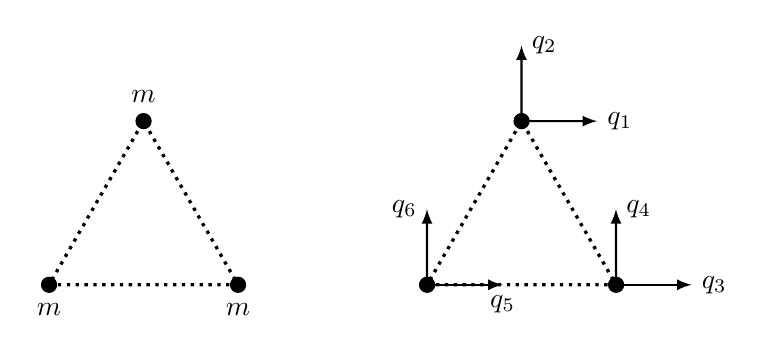
\begin{tikzpicture}[>=latex,scale=1.2]
			\coordinate (A) at (0,0);
			\coordinate (B) at (2,0);
			\coordinate (C) at (1,1.732);

			\draw[fill=black] (A) circle (0.08);
			\draw[fill=black] (B) circle (0.08);
			\draw[fill=black] (C) circle (0.08);
			\draw[dotted,very thick] (A) node[below=1mm]{\(m\)}--(B) node[below=1mm]{\(m\)}--(C)node[above=1mm]{\(m\)}--(A);

			\coordinate (D) at (4,0);
			\coordinate (E) at (6,0);
			\coordinate (F) at (5,1.732);

			\draw[fill=black] (D) circle (0.08);
			\draw[fill=black] (E) circle (0.08);
			\draw[fill=black] (F) circle (0.08);
			\draw[dotted,very thick] (D)--(E)--(F)--(D);
			\draw[thick,->] (F)--(5.8,1.732) node[right]{\(q_1\)};
			\draw[thick,->] (F)--(5,2.532) node[right]{\(q_2\)};
			\draw[thick,->] (E)--(6.8,0) node[right]{\(q_3\)};
			\draw[thick,->] (E)--(6,0.8) node[right]{\(q_4\)};
			\draw[thick,->] (D)--(4.8,0) node[below]{\(q_5\)};
			\draw[thick,->] (D)--(4,0.8) node[left]{\(q_6\)};
		\end{tikzpicture}
	\end{figure}

	Taking the centre of mass as the origin, we have
	\[\vb{x}_1=l\qty(0,\frac{1}{\sqrt{3}})+(q_1,q_2)\,,\]
	\[\vb{x}_2=l\qty(\frac{1}{2},-\frac{1}{2\sqrt{3}})+(q_3,q_4)\,,\]
	\[\vb{x}_3=l\qty(-\frac{1}{2},-\frac{1}{2\sqrt{3}})+(q_5,q_6)\,.\]

	The kinetic energy is
	\[T=\frac{1}{2}m(\dot{\vb{x}}_1^2+\dot{\vb{x}}_2^2+\dot{\vb{x}}_3^2)=\frac{1}{2}m(\dot{q}_1^2+\dot{q}_2^2+\dot{q}_3^2+\dot{q}_4^2+\dot{q}_5^2+\dot{q}_6^2)\,,\]
	so the matrix \(\mathsf{T}\) is diagonal:
	\[T_{ij}=m\delta_{ij}\,.\]

	The potential energy is
	\[V=\frac{1}{2}k[(\abs{\vb{x}_1-\vb{x}_2}-l)^2+(\abs{\vb{x}_2-\vb{x}_3}-l)^2+(\abs{\vb{x}_3-\vb{x}_1}-l)^2]\,.\]
	Assume small oscillations. We can write, say,
	\begin{align*}
		\vb{x}_1-\vb{x}_2&=l\qty(-\frac{1}{2},\frac{\sqrt{3}}{2})+(q_1-q_3,q_2-q_4)\\
		&=\vb{z}+\bm{\epsilon}\,,
	\end{align*}
	where \(l=\abs{\vb{z}}\gg \abs{\bm{\epsilon}}\). Taylor expansion gives
	\[\abs{\vb{z}+\bm{\epsilon}}=\sqrt{\vb{z}\vdot\vb{z}+2\vb{z}\vdot\bm{\epsilon}+\bm{\epsilon}\vdot\bm{\epsilon}}\approx l\qty(1+\frac{\vb{z}\vdot\bm{\epsilon}}{l^2})\,.\]
	Hence, the potential energy is expanded to
	\[V=\frac{k}{2}\qty[-\frac{1}{2}(q_1-q_3)+\frac{\sqrt{3}}{2}(q_2-q_4)]^2+\frac{k}{2}(q_3-q_5)^2+\frac{k}{2}\qty[-\frac{1}{2}(q_5-q_1)-\frac{\sqrt{3}}{2}(q_6-q_2)]^2\,,\]
	and so the matrix \(\mathsf{V}\) is given by
	\[\mathsf{V}=\frac{k}{4}\begin{pmatrix}
		2 & 0 & -1 & \sqrt{3} & -1 & -\sqrt{3}\\
		0 & 6 & \sqrt{3} & -3 & -\sqrt{3} & -3\\
		-1 & \sqrt{3} & 5 & -\sqrt{3} & -4 & 0\\
		\sqrt{3} & -3 & -\sqrt{3} & 3 & 0 & 0\\
		-1 & -\sqrt{3} & -4 & 0 & 5 & \sqrt{3}\\
		-\sqrt{3} & -3 & 0 & 0 & \sqrt{3} & 3\\
	\end{pmatrix}\,.\]

	Solving the characteristic equation
	\[\det(\mathsf{V}-\omega^2\mathsf{T})=0\]
	is too tedious in this case. However, we can guess most of the normal modes using the symmetries of the problem.

	First of all, there are some zero modes, corresponding to the non-oscillatory rigid motions. The system can translate in two dimensions:
	\[\vb{Q}^{(1)}=\begin{pmatrix}
		1 \\ 0 \\ 1 \\ 0 \\ 1 \\ 0
	\end{pmatrix}\text{ and }\vb{Q}^{(2)}=\begin{pmatrix}
		0 \\ 1 \\ 0 \\ 1 \\ 0 \\ 1
	\end{pmatrix}\,.\]
	Similarly, the system can rotate about its centre:
	\[\vb{Q}^{(3)}=\begin{pNiceMatrix}
		1 \\ 0 \\ -\frac{1}{2} \\ -\frac{\sqrt{3}}{2} \\ -\frac{1}{2} \\ \frac{\sqrt{3}}{2}
	\end{pNiceMatrix}\,.\]

	By symmetry, we expect there would be a mode where the masses expand and contract at the same frequency in the radial direction. This is expressed by the eigenvector
	\[\vb{Q}^{(4)}=\begin{pNiceMatrix}
		0 \\ 1 \\ \frac{\sqrt{3}}{2} \\ -\frac{1}{2} \\ -\frac{\sqrt{3}}{2} \\ -\frac{1}{2}
	\end{pNiceMatrix}\,,\]
	which has a normal frequency of \(\omega^2=\frac{3k}{m}\).

	For a mode with reflection symmetry, we can try the form
	\[\vb{Q}^{(5)}=\begin{pmatrix}
		0 \\ -1 \\ \beta \\ \gamma \\ -\beta \\ \gamma
	\end{pmatrix}\,,\]
	which works with \(\beta=\frac{\sqrt{3}}{2}\) and \(\gamma=\frac{1}{2}\), and the normal frequency can be found out to be \(\omega^2=\frac{3k}{2m}\).

	Using orthogonality, we can find out the last normal mode:
	\[\vb{Q}^{(6)}=\begin{pNiceMatrix}
		1 \\ 0 \\ -\frac{1}{2} \\ \frac{\sqrt{3}}{2} \\ -\frac{1}{2} \\ -\frac{\sqrt{3}}{2}
	\end{pNiceMatrix}\,,\]
	with \(\omega^2=\frac{3k}{2m}\).
	\subsection{Normal Modes and Group Representations}
	Consider an oscillating system with the Lagrangian of the form
	\[L=\frac{1}{2}\dot{\mathsf{q}}\tp\mathsf{T}\dot{\mathsf{q}}-\frac{1}{2}\mathsf{q}\tp\mathsf{Vq}\,.\]
	If the system has a symmetry group \(G\), then the action of a symmetry transformation \(g\in G\) on the vector of generalised coordinates is
	\[\vb{q}\to\rho(g)\mathsf{q}\,.\]
	If \(\vb{q}\) has \(N\) components, then \(\rho\) is an \(N\)-dimensional representation of \(G\). Since \(g\) is a symmetry operation on the system, the kinetic and potential energies must transform so that \(L\) is invariant. For all \(g\in G\),
	\[\begin{cases}
		\rho(g)\tp\mathsf{T}\rho(g)=\mathsf{T}\\
		\rho(g)\tp\mathsf{V}\rho(g)=\mathsf{V}\,.
	\end{cases}\]
	By Weyl's unitary trick (\cref{weyltrick}), we can always find a basis such that all the representations \(\rho(g)\) are unitary. Since the coordinates are real, we can choose such a basis so that \(\rho(g)\) are orthogonal, and
	\begin{equation}\tag{\(\dagger\)}
		\begin{cases}
			\rho(g)^{-1}\mathsf{T}\rho(g)=\mathsf{T}\\
			\rho(g)^{-1}\mathsf{V}\rho(g)=\mathsf{V}\,.
		\end{cases}
	\end{equation}
	Often the representation \(\rho\) is reducible, so the matrices \(\rho(g)\) may be transformed into block-diagonal form by a similarity transformation
	\[\mathsf{S}\rho(g)\mathsf{S}^{-1}=\begin{pmatrix}
		\phi^{(1)}(g) & \mathsf{0} & \cdots & \mathsf{0}\\
		\mathsf{0} & \phi^{(2)}(g) & \cdots & \mathsf{0}\\
		\vdots & \vdots & \ddots & \mathsf{0}\\
		\mathsf{0} & \mathsf{0} & \cdots & \phi^{(k)}(g)
	\end{pmatrix}\,.\]
	For simplicity, let us assume here that each of the irreducible representations \(\phi^{(i)}\) are different from each other. Note that the matrices along the diagonal are square, of dimensions \(\{n_\alpha\}_{\alpha=1}^{k}\). Transform equations (\(\dagger\)), we have
	\begin{align*}
		&\begin{cases}
			\mathsf{S}\rho(g)^{-1}\mathsf{T}\rho(g)\mathsf{S}^{-1}=\mathsf{S}\mathsf{T}\mathsf{S}^{-1}\\
			\mathsf{S}\rho(g)^{-1}\mathsf{V}\rho(g)\mathsf{S}^{-1}=\mathsf{S}\mathsf{V}\mathsf{S}^{-1}
		\end{cases}\\
		\implies &\begin{cases}
			(\mathsf{S}\mathsf{T}\mathsf{S}^{-1})(\mathsf{S}\rho(g)\mathsf{S}^{-1})=(\mathsf{S}\rho(g)\mathsf{S}^{-1})(\mathsf{S}\mathsf{T}\mathsf{S}^{-1})\\
			(\mathsf{S}\mathsf{V}\mathsf{S}^{-1})(\mathsf{S}\rho(g)\mathsf{S}^{-1})=(\mathsf{S}\rho(g)\mathsf{S}^{-1})(\mathsf{S}\mathsf{V}\mathsf{S}^{-1})\,.
		\end{cases}
	\end{align*}
	Rewriting \(\tilde{\mathsf{T}}=\mathsf{S}\mathsf{T}\mathsf{S}^{-1}\) and \(\tilde{\mathsf{V}}=\mathsf{S}\mathsf{V}\mathsf{S}^{-1}\), and since \(\mathsf{S}\rho(g)\mathsf{S}^{-1}\) is block diagonal, we have
	\begin{align*}
		\tilde{\mathsf{T}}(\mathsf{S}\rho(g)\mathsf{S}^{-1})&=\begin{pmatrix}
			\mathsf{T}^{(11)} & \mathsf{T}^{(12)} & \cdots & \mathsf{T}^{(1k)}\\
			\mathsf{T}^{(21)} & \mathsf{T}^{(22)} & \cdots & \mathsf{T}^{(2k)}\\
			\vdots & \vdots & \ddots & \vdots\\
			\mathsf{T}^{(k1)} & \mathsf{T}^{(k2)} & \cdots & \mathsf{T}^{(kk)}
		\end{pmatrix}\begin{pmatrix}
			\phi^{(1)}(g) & \mathsf{0} & \cdots & \mathsf{0}\\
			\mathsf{0} & \phi^{(2)}(g) & \cdots & \mathsf{0}\\
			\vdots & \vdots & \ddots & \mathsf{0}\\
			\mathsf{0} & \mathsf{0} & \cdots & \phi^{(k)}(g)
		\end{pmatrix}\\
		&=\begin{pmatrix}
			\mathsf{T}^{(11)}\phi^{(1)}(g) & \mathsf{T}^{(12)}\phi^{(2)}(g) & \cdots & \mathsf{T}^{(1k)}\phi^{(k)}(g)\\
			\mathsf{T}^{(21)}\phi^{(1)}(g) & \mathsf{T}^{(22)}\phi^{(2)}(g) & \cdots & \mathsf{T}^{(2k)}\phi^{(k)}(g)\\
			\vdots & \vdots & \ddots & \vdots\\
			\mathsf{T}^{(k1)}\phi^{(1)}(g) & \mathsf{T}^{(k2)}\phi^{(2)}(g) & \cdots & \mathsf{T}^{(kk)}\phi^{(k)}(g)
		\end{pmatrix}\,,
	\end{align*}
	\begin{align*}
		(\mathsf{S}\rho(g)\mathsf{S}^{-1})\tilde{\mathsf{T}}&=\begin{pmatrix}
			\phi^{(1)}(g) & \mathsf{0} & \cdots & \mathsf{0}\\
			\mathsf{0} & \phi^{(2)}(g) & \cdots & \mathsf{0}\\
			\vdots & \vdots & \ddots & \mathsf{0}\\
			\mathsf{0} & \mathsf{0} & \cdots & \phi^{(k)}(g)
		\end{pmatrix}\begin{pmatrix}
			\mathsf{T}^{(11)} & \mathsf{T}^{(12)} & \cdots & \mathsf{T}^{(1k)}\\
			\mathsf{T}^{(21)} & \mathsf{T}^{(22)} & \cdots & \mathsf{T}^{(2k)}\\
			\vdots & \vdots & \ddots & \vdots\\
			\mathsf{T}^{(k1)} & \mathsf{T}^{(k2)} & \cdots & \mathsf{T}^{(kk)}
		\end{pmatrix}\\
		&=\begin{pmatrix}
			\phi^{(1)}(g)\mathsf{T}^{(11)} & \phi^{(1)}(g)\mathsf{T}^{(12)} & \cdots & \phi^{(1)}(g)\mathsf{T}^{(1k)}\\
			\phi^{(2)}(g)\mathsf{T}^{(21)} & \phi^{(2)}(g)\mathsf{T}^{(22)} & \cdots & \phi^{(2)}(g)\mathsf{T}^{(2k)}\\
			\vdots & \vdots & \ddots & \vdots\\
			\phi^{(k)}(g)\mathsf{T}^{(k1)} & \phi^{(k)}(g)\mathsf{T}^{(k2)} & \cdots & \phi^{(k)}(g)\mathsf{T}^{(kk)}\\
		\end{pmatrix}\,.
	\end{align*}
	Therefore, we must have
	\[\mathsf{T}^{(\alpha\beta)}\phi^{(\beta)}(g)=\phi^{(\alpha)}(g)\mathsf{T}^{(\alpha\beta)}\,.\]
	If the block diagonal elements of \(\mathsf{S}\rho(g)\mathsf{S}^{-1}\) are different, then by Schur's Lemma (\cref{schur}),
	\[\begin{cases}
		\tilde{\mathsf{T}}^{(\alpha\beta)}=t_\alpha\delta_{\alpha\beta}\mathsf{I}_\alpha\\
		\tilde{\mathsf{V}}^{(\alpha\beta)}=v_\alpha\delta_{\alpha\beta}\mathsf{I}_\alpha\,,
	\end{cases}\]
	where \(t_i,v_i\in\mathbb{R}\), and \(\mathsf{I}_i\) is the \(n_i\times n_i\) identity matrix.
	Therefore,
	\[\mathsf{STS}^{-1}=\begin{pmatrix}
		t_1\mathsf{I}_1 & \mathsf{0} & \cdots & \mathsf{0}\\
		\mathsf{0} & t_2\mathsf{I}_2 & \cdots & \mathsf{0}\\
		\vdots & \vdots & \ddots & \vdots\\
		\mathsf{0} & \mathsf{0} & \cdots & t_k\mathsf{I}_k\,,
	\end{pmatrix}\]
	\[\mathsf{SVS}^{-1}=\begin{pmatrix}
		v_1\mathsf{I}_1 & \mathsf{0} & \cdots & \mathsf{0}\\
		\mathsf{0} & v_2\mathsf{I}_2 & \cdots & \mathsf{0}\\
		\vdots & \vdots & \ddots & \vdots\\
		\mathsf{0} & \mathsf{0} & \cdots & v_k\mathsf{I}_k
	\end{pmatrix}\,.\]

	Once the kinetic and potential energy matrices are diagonalised in this way, finding the normal modes is straightforward. The normal frequencies are
	\[\omega_\alpha^2=\frac{v_\alpha}{t_\alpha}\]
	with degeneracy \(n_\alpha\). The generalised eigenvectors of normal modes span the invariant subspace of the underlying vector space acted on by the corresponding irreducible representation of the symmetry group.

	If an irreducible representation \(\phi^{(\alpha)}(g)\) occurs with multiplicity \(m_\alpha >1\), then the corresponding diagonal block of \(t_\alpha\) and \(v_\alpha\) are replaced by an \(m_\alpha\times m_\alpha\) block matrix. \(\mathsf{T}\) and \(\mathsf{V}\) are not completely diagonal, but finding the normal modes reduces to solving separate generalised eigenvalue problems for each \(\alpha\).

	\subsubsection{Example: CO\(_2\) Molecule Revisited}
	We will, again, only consider the 1D motions of the atoms in a CO\(_2\) molecule. Its symmetry group is therefore \(G=\{I,m\}\). The action of the group on the coordinates \(\vb{q}=(x_1,x_2,x_3)\) is given by the representation \(\phi\), where
	\begin{align*}
		&\phi(I)\begin{pmatrix}
			x_1 \\ x_2 \\x_3
		\end{pmatrix}=\begin{pmatrix}
			x_1 \\ x_2 \\ x_3
		\end{pmatrix}\quad & &\implies \quad \phi(I)=\begin{pmatrix}
			1 & 0 & 0\\
			0 & 1 & 0\\
			0 & 0 & 1
		\end{pmatrix}\,,\\
		&\phi(m)\begin{pmatrix}
			x_1 \\ x_2 \\x_3
		\end{pmatrix}=\begin{pmatrix}
			-x_3 \\ -x_2 \\ -x_1
		\end{pmatrix}\quad & &\implies \quad \phi(m)=\begin{pmatrix}
			0 & 0 & -1\\
			0 & -1 & 0\\
			-1 & 0 & 0
		\end{pmatrix}\,.
	\end{align*}
	The character of this representation is
	\[\chi_\phi(I)=3\,,\;\chi_\phi(m)=-1\,.\]

	The character table of this group is
	\begin{center}
		\begin{TAB}(b,22pt,16pt)[3pt]{c|c|c}{c|cc}
			\(G\) & \(I\) & \(m\) \\
			\(\chi_{\rho^{(1)}}\) & \(1\) & \(1\)\\
			\(\chi_{\rho^{(2)}}\) & \(1\) & \(-1\)\\
		\end{TAB}
	\end{center}
	so the representation is decomposed into
	\[\phi=\rho^{(1)}\oplus 2\rho^{(2)}\,.\]
	This corresponds to the single symmetric mode (\(\vb{Q}^{(2)}\)) and two anti-symmetric modes (\(\vb{Q}^{(1)}\) and \(\vb{Q}^{(3)}\)) as seen before.
	\subsubsection{Example: Equilateral Triangle Revisited}
	Consider the 2D vibration of an equilateral triangle, which belongs to the symmetry group \(D_3=\{I,R,R^2,m_1,m_2,m_3\}\). Using the coordinate as before, we can find out the representation
	\[\phi(I)=\begin{pmatrix}
		1 & 0 & 0 & 0 & 0 & 0\\
		0 & 1 & 0 & 0 & 0 & 0\\
		0 & 0 & 1 & 0 & 0 & 0\\
		0 & 0 & 0 & 1 & 0 & 0\\
		0 & 0 & 0 & 0 & 1 & 0\\
		0 & 0 & 0 & 0 & 0 & 1
	\end{pmatrix}\,,\]
	\[\phi(m_1)=\begin{pmatrix}
		-1 & 0 & 0 & 0 & 0 & 0\\
		0 & 1 & 0 & 0 & 0 & 0\\
		0 & 0 & 0 & 0 & -1 & 0\\
		0 & 0 & 0 & 0 & 0 & 1\\
		0 & 0 & -1 & 0 & 0 & 0\\
		0 & 0 & 0 & 1 & 0 & 0\\
	\end{pmatrix}\,,\]
	\[\phi(R)=\begin{pmatrix}
		0 & 0 & 0 & 0 & \frac{1}{2} & \frac{\sqrt{3}}{2}\\
		0 & 0 & 0 & 0 & -\frac{\sqrt{3}}{2} & -\frac{1}{2}\\
		\frac{1}{2} & \frac{\sqrt{3}}{2} & 0 & 0 & 0 & 0\\
		-\frac{\sqrt{3}}{2} & -\frac{1}{2} & 0 & 0 & 0 & 0\\
		0 & 0 & \frac{1}{2} & \frac{\sqrt{3}}{2} & 0 & 0\\
		0 & 0 & -\frac{\sqrt{3}}{2} & -\frac{1}{2} & 0 & 0
	\end{pmatrix}\,,\]
	with character
	\[\chi_\phi(I)=6\,,\;\chi_\phi(m_1)=0\,,\;\chi_\phi(R)=0\,.\]

	We have the character table of \(D_3\):
	\begin{center}
		\begin{TAB}(b,22pt,16pt)[2pt]{c|c|cc|ccc}{c|ccc}
			\(D_3\) & \(I\) & \(R\) & \(R^2\) & \(m_1\) & \(m_2\) & \(m_3\)\\
			\(\chi_{\rho^{(1)}}\) & \(1\) & \(1\) & \(1\) & \(1\) & \(1\) & \(1\)\\
			\(\chi_{\rho^{(2)}}\) & \(1\) & \(1\) & \(1\) & \(-1\) & \(-1\) & \(-1\)\\
			\(\chi_{\rho^{(3)}}\) & \(2\) & \(-1\) & \(-1\) & \(0\) & \(0\) & \(0\)
		\end{TAB}
	\end{center}
	and the representation is decomposed as
	\[\phi=\rho^{(1)}\oplus\rho^{(2)}\oplus 2\rho^{(3)}\,.\]

	The trivial representation \(\rho^{(1)}\) is the symmetric breathing mode (\(\vb{Q}^{(4)}\)). \(\rho^{(2)}\) corresponds to the rigid rotation (\(\vb{Q}^{(3)}\)) since it is unchanged by \(R\), but reversed by \(m\). The two translations (\(\vb{Q}^{(1)}\) and \(\vb{Q}^{(2)}\)) corresponds to a two-dimensional irreducible representation \(\rho^{(3)}\). The final \(\rho^{(3)}\) corresponds to another pair of degenerate non-zero modes (\(\vb{Q}^{(5)}\) and \(\vb{Q}^{(6)}\)).

	This is demonstrated by the transformations of the normal mode eigenvectors. For the two translational modes (\(\vb{Q}^{(1)}\) and \(\vb{Q}^{(2)}\)), we have
	\begin{align*}
		\rho(m_1)\begin{pmatrix}
			| & |\\
			\vb{Q}^{(1)} & \vb{Q}^{(2)}\\
			| & |
		\end{pmatrix}&=\begin{pmatrix}
			| & |\\
			\vb{Q}^{(1)} & \vb{Q}^{(2)}\\
			| & |
		\end{pmatrix}\begin{pmatrix}
			-1 & 0\\
			0 & 1
		\end{pmatrix}\,,\\
		\rho(R)\begin{pmatrix}
			| & |\\
			\vb{Q}^{(1)} & \vb{Q}^{(2)}\\
			| & |
		\end{pmatrix}&=\begin{pmatrix}
			| & |\\
			\vb{Q}^{(1)} & \vb{Q}^{(2)}\\
			| & |
		\end{pmatrix}\begin{pmatrix}
			-\frac{1}{2} & \frac{\sqrt{3}}{2}\\
			-\frac{\sqrt{3}}{2} & -\frac{1}{2}
		\end{pmatrix}\,.
	\end{align*}
	The other pair of doubly degenerate modes \(\begin{pmatrix}\vb{Q}^{(6)}&\vb{Q}^{(5)}\end{pmatrix}\) transforms just as \(\begin{pmatrix}\vb{Q}^{(1)}&\vb{Q}^{(2)}\end{pmatrix}\). For the rotation and dilation modes, we have
	\begin{align*}
		\rho(m_1)\vb{Q}^{(3)}&=-\vb{Q}^{(3)}\,, \\
		\rho(R)\vb{Q}^{(3)}&=\vb{Q}^{(3)}\,, \\
		\rho(m_1)\vb{Q}^{(4)}&=\vb{Q}^{(4)}\,, \\
		\rho(R)\vb{Q}^{(4)}&=\vb{Q}^{(4)}\,.
	\end{align*}
\end{document}
